\documentclass[10pt]{book} 

\input{structure} 

\begin{document}

%----------------------------------------------------------------------------------------
%	Apuntes teoría Cuántica de Campos
%----------------------------------------------------------------------------------------

\begingroup
\thispagestyle{empty}
\begin{tikzpicture}[remember picture,overlay]
\coordinate [below=12cm] (midpoint) at (current page.north);
\node at (current page.north west)
{\begin{tikzpicture}[remember picture,overlay]
\node[anchor=north west,inner sep=0pt] at (0,0) {
\includegraphics[width=\paperwidth]{background}}; % Background image
\draw[anchor=north] (midpoint) node [fill=ocre!30!white,fill opacity=0.6,text opacity=1,inner sep=1cm]{\Huge\centering\bfseries\sffamily\parbox[c][][t]{\paperwidth}{\centering Teoría Cuántica de Campos y temas selectos de física de partículas\\[15pt] % Book title
{\Large E. Rojas, O. Rosero, L. Rozo}\\[20pt] % Subtitle
{\huge }}}; % Author name
\end{tikzpicture}};
\end{tikzpicture}
\vfill
\endgroup

%----------------------------------------------------------------------------------------
%	COPYRIGHT PAGE
%----------------------------------------------------------------------------------------

\newpage
~\vfill
\thispagestyle{empty}

\noindent DERECHOS RESERVADOS \copyright\ 2021\\ % Copyright notice

\noindent \textsc{Published by Universidad de Nariño}\\ % Publisher

\noindent \textsc{book-website.com}\\ % URL

\noindent Licensed under the Creative Commons Attribution-NonCommercial 3.0 Unported License (the ``License''). You may not use this file except in compliance with the License. You may obtain a copy of the License at \url{http://creativecommons.org/licenses/by-nc/3.0}. Unless required by applicable law or agreed to in writing, software distributed under the License is distributed on an \textsc{``as is'' basis, without warranties or conditions of any kind}, either express or implied. See the License for the specific language governing permissions and limitations under the License.\\ % License information

\noindent \textit{First printing, July 2021} % Printing/edition date

%----------------------------------------------------------------------------------------
%	TABLE OF CONTENTS
%----------------------------------------------------------------------------------------

%\usechapterimagefalse % If you don't want to include a chapter image, use this to toggle images off - it can be enabled later with \usechapterimagetrue

\chapterimage{chapter_head_0.pdf} % Table of contents heading image
\pagestyle{empty} % No headers
\tableofcontents % Print the table of contents itself
\cleardoublepage % Forces the first chapter to start on an odd page so it's on the right
\pagestyle{fancy} % Print headers again
%----------------------------------------------------------------------------------------
\part{Teoría cuántica de campos}
%	CAPITULOS
%----------------------------------------------------------------------------------------

%----------------------------------------------------------------------------------------
%	CHAPTER 1 Introducción

%----------------------------------------------------------------------------------------
%	CHAPTER 1 Introducción
%----------------------------------------------------------------------------------------

\chapterimage{chapter_head_2.pdf} % Chapter heading image

\chapter{Introducción}

La era de la mec\'{a}nica cu\'{a}ntica comenz\'{o} cuando Planck postul\'{o} que los modos de radiaci\'{o}n de frecuencia angular $\omega $ pod\'{\i}an contarse como part\'{\i}culas con energ\'{\i}a $E=\hbar \omega $, y deriv\'{o} la ley de radiaci\'{o}n de cuerpo negro sin llegar a infinitos. Las implicaciones f\'{\i}sicas de este postulado fundamental se hicieron m\'{a}s claras cuando Einstein mostr\'{o} que la cuantificaci\'{o}n de la radiaci\'{o}n tambi\'{e}n explicaba la dependencia de la frecuencia del efecto fotoel\'{e}ctrico. Esto pronto condujo a una proliferaci\'{o}n de nuevas ideas gracias a Bohr, Dirac, Born, Schr\"{o}dinger, Heisenberg y muchos otros, quienes aplicaron la idea de cuantificaci\'{o}n a part\'{\i}culas y encontraron un \'{e}xito notable en la descripci\'{o}n de fen\'{o}menos subat\'{o}micos. Dirac incluso construy\'{o} una teor\'{\i}a relativista del electr\'{o}n, que estaba en excelente acuerdo con los experimentos subat\'{o}micos. A pesar de su \'{e}xito, hubo algunas deficiencias esenciales de la mec\'{a}nica cu\'{a}ntica de part\'{\i}culas.

\section{\textquestiondown Porqu\'{e} una teoría Cu\'{a}ntica de Campos?}

Una de estas deficiencias fue filos\'{o}fica. La mec\'{a}nica cu\'{a}ntica comenz\'{o} con la descripci\'{o}n de la luz en t\'{e}rminos de fotones, pero la descripci\'{o}n cl\'{a}sica de la luz fue en t\'{e}rminos de propagaci\'{o}n de campos electromagn\'{e}ticos. Entonces, una teor\'{\i}a de los fotones requer\'{\i}a una receta de c\'{o}mo cuantificar campos, un eslab\'{o}n perdido entre las dos descripciones. Como se ver\'{a} en los pr\'{o}ximos cap\'{\i}tulos, la estructura necesaria para cuantificar los campos electromagn\'{e}ticos se puede utilizar para describir todas las part\'{\i}culas elementales como campos cu\'{a}nticos. Incluso se encontr\'{o} que la ecuaci\'{o}n de onda relativista de Dirac ten\'{\i}a la descripci\'{o}n m\'{a}s simple en t\'{e}rminos de campos cu\'{a}nticos que representan electrones y positrones.

Otro problema de la mec\'{a}nica cu\'{a}ntica de part\'{\i}culas es que, por definici\'{o}n, es v\'{a}lida en el r\'{e}gimen no relativista. Esto se debe s\'{o}lo a que utiliza hamiltonianos no relativistas para resolver varios problemas. De hecho, todo el dise\~{n}o de la mec\'{a}nica cu\'{a}ntica no relativista desaf\'{\i}a la relatividad. Por ejemplo, utiliza el concepto de potenciales, que es insostenible en cualquier teoría relativista ya que supone la transferencia de informaci\'{o}n a una velocidad infinita. Además, el espacio y el tiempo se tratan de manera muy diferente en la mecánica cu\'{a}ntica no relativista. Las coordenadas espaciales son operadores, mientras que el tiempo es un par\'{a}metro, y normalmente estudiamos la evoluci\'{o}n de diferentes operadores, incluidas las coordenadas espaciales, en el tiempo. La ecuaci\'{o}n de Dirac, aunque covariante, trata el espacio y el tiempo en bases diferentes. En una teoría verdaderamente relativista, el espacio y el tiempo deberían fusionarse en un espacio-tiempo, y no se puede hacer una distinci\'{o}n tan fundamental entre la parte espacial y la parte temporal.

Tambi\'{e}n hay un problema pr\'{a}ctico. En la naturaleza existen procesos en los que se crean o aniquilan nuevas part\'{\i}culas. Por ejemplo el decaimiento $\beta $ se puede considerar como la desintegraci\'{o}n de un neutr\'{o}n en un prot\'{o}n, un electr\'{o}n y un antineutrino:

\begin{equation}
n\rightarrow p+e^{-}+\overline{\nu }_{e}  \label{1}
\end{equation}

El neutr\'{o}n se aniquila en este proceso, mientras que se crean el prot\'{o}n, el electr\'{o}n, etc. La mec\'{a}nica cu\'{a}ntica de part\'{\i}culas se ocupa de las part\'{\i}culas estables y sus movimientos en varios potenciales. Sin cuantificaci\'{o}n de campos, cualquier c\'{a}lculo que implique la creaci\'{o}n o aniquilaci\'{o}n de part\'{\i}culas es totalmente err\'{o}neo. La teor\'{\i}a cu\'{a}ntica de campos, al incorporar la creaci\'{o}n y aniquilaci\'{o}n de cuantos o part\'{\i}culas como su caracter\'{\i}stica esencial, permiti\'{o} c\'{a}lculos significativos de resultados verificables experimentalmente. Cuando uno pasa al r\'{e}gimen relativista, se encuentra con la posibilidad de crear nuevas part\'{\i}culas a partir de la energ\'{\i}a. Por ejemplo, si un electr\'{o}n y un positr\'{o}n chocan con suficiente energ\'{\i}a, el proceso de colisi\'{o}n puede crear pares extra de electrones y positrones:

\begin{equation}
e^{-}+e^{+}\rightarrow e^{-}+e^{+}+e^{-}+e^{+}  \label{2}
\end{equation}

Esto, por supuesto, puede suceder s\'{o}lo si la energ\'{\i}a cin\'{e}tica total inicial del par $e^{-}~e^{+}$ es mayor que la energ\'{\i}a de masa en reposo del par adicional que se va a crear. Para permitir tales posibilidades, se requiere alg\'{u}n mecanismo para describir la creaci\'{o}n de part\'{\i}culas. Incluso cuando los estados inicial y final de un problema involucran las mismas part\'{\i}culas, un proceso cu\'{a}ntico puede pasar por estados intermedios que involucran a otras part\'{\i}culas que se crean y destruyen en el proceso. Tales estados intermedios pueden contribuir a la amplitud del proceso y afectar el resultado. Es importante considerar estas posibilidades cuando se quiere hacer pruebas de precisi\'{o}n de la teor\'{\i}a cu\'{a}ntica. La creaci\'{o}n y aniquilaci\'{o}n de las part\'{\i}culas intermedias en tales casos s\'{o}lo puede manejarse pasando a la teor\'{\i}a cu\'{a}ntica de campos.


\section{Operadores Aniquilador y Creador}

\newcommand{\Oaa}{\hat{a}}

Ahora, recordando un problema de la mec\'{a}nica cu\'{a}ntica no relativista que puede resolverse mediante la introducci\'{o}n de operadores que crean y aniquilan los cuantos, es el problema del oscilador arm\'{o}nico simple. Aqu\'{\i} se revisa este tema, ya que ser\'{a} muy \'{u}til para desarrollar la teor\'{\i}a cu\'{a}ntica de campos en los cap\'{\i}tulos siguientes.

El hamiltoniano cuantizado del oscilador unidimensional viene dado por,

\begin{equation}
\hat{H}=\frac{1}{2m}\left( \hat{P}^{2}+m^{2}\omega ^{2}\hat{X}^{2}\right) =%
\frac{\hbar \omega }{2}\left( \frac{\hat{P}^{2}}{m\hbar \omega }+\frac{%
m\omega }{\hbar }\hat{X}^{2}\right)  \label{3}
\end{equation}

\begin{exercise}
Demostrar que el Hamiltoniano asociado al oscilador armónico cuántico se lo puede escribir en términos de los operadores aniquilador y creador de la siguiente manera
\begin{equation*}
\hat{H}=\frac{\hbar \omega }{2}\left[ \Oaa^{\dagger }\Oaa+\Oaa \Oaa^{\dagger }\right] 
\end{equation*}
\end{exercise} 

\newcommand{\Op}{\hat{p}}
\newcommand{\Ox}{\hat{x}}
\newcommand{\OP}{\hat{P}}
\newcommand{\OX}{\hat{X}}

\begin{solution}
Se define las siguientes combinaciones de operadores adimensionales \emph{(Recordar que} $\hbar \omega$ \emph{\ posee unidades de energ\'{\i}a)}:

\begin{equation*}
\hat{p}=\frac{1}{\sqrt{m\hbar \omega }}\OP \qquad ;\qquad  \hat{x}=\sqrt{\frac{m\omega }{\hbar}}\OX
\end{equation*}

Reemplazando en la ecuaci\'{o}n (\ref{3}) asociada a $\hat{H}$

\begin{equation}
\hat{H}=\frac{\hbar \omega }{2}\left( \Op^{2}+\Ox^{2}\right)  \label{1.3}
\end{equation}

Con el fin de redefinir el Hamiltoniano de la l\'{\i}nea (\ref{1.3}), definir los siguientes operadores

\begin{equation}
\Oaa \equiv \frac{1}{\sqrt{2}}\left( \Op-\ii \Ox \right) \qquad ;\qquad \Oaa^{\dagger } \equiv \frac{1}{\sqrt{2}}\left( \Op+\ii \Ox\right)  \label{1.3A}
\end{equation}

que escrito en t\'{e}rminos de los operadores $\OX$ y \thinspace $\OP$ se reducen a

\begin{eqnarray*}
\Oaa &=&\frac{1}{\sqrt{2}}\left( \Op-\ii \Ox \right) =\frac{1}{\sqrt{2}}\left( \frac{1}{\sqrt{m\hbar \omega }} \OP- \ii \sqrt{\frac{m\omega }{\hbar }}\OX \right) =\frac{1}{\sqrt{2m\hbar \omega }}\left( \OP-\ii \sqrt{\frac{m\omega}{\hbar}}\sqrt{m\hbar \omega} \OX \right) \\
&=&\frac{1}{\sqrt{2m\hbar \omega }}\left( \OP-\ii m\omega \OX \right),
\end{eqnarray*}

en tanto que

\begin{eqnarray*}
\Oaa^{\dagger } &=& \frac{1}{\sqrt{2}}\left( \Op+ \ii \Ox\right) =\frac{1}{\sqrt{2}}\left( \frac{1}{\sqrt{m\hbar \omega }} \OP + \ii \sqrt{\frac{m\omega }{\hbar}} \OX \right) =\frac{1}{\sqrt{2m\hbar \omega }}\left( \OP+\ii \sqrt{\frac{m\omega}{\hbar}}\sqrt{m\hbar \omega } \OX \right) \\
&=&\frac{1}{\sqrt{2m\hbar \omega }}\left( \OP+\ii m\omega \OX \right), 
\end{eqnarray*}

concluyendo
\begin{equation}
\boxed{
\Oaa \equiv \frac{1}{\sqrt{2m\hbar \omega }}\left( \OP-\ii m\omega \OX \right) \qquad ;\qquad \Oaa^{\dagger }=\frac{1}{\sqrt{2m\hbar \omega }}\left( \OP+\ii m\omega \OX\right).}  \label{1.4}
\end{equation}

\noindent
Por otro lado, es necesario calcular las siguientes relaciones a partir de (\ref{1.3A}):

\vspace{0.2cm}
\noindent
\begin{itemize}
\item[$i)$]
\begin{eqnarray}
\Oaa+\Oaa^{\dagger } &=& \frac{1}{\sqrt{2}}\left( \Op+\ii \Ox \right) +\frac{1}{\sqrt{2}}\left( \Op-\ii \Ox \right) =\frac{1}{\sqrt{2}}\left( \Op+\ii \Ox +\Op - \ii \Ox \right) =\frac{2p}{\sqrt{2}}  \notag \\
&\therefore &~\ \Op=\frac{\sqrt{2}}{2}\left( \Oaa+\Oaa^{\dagger }\right) \quad \text{ó} \quad  \OP =  \sqrt{\frac{m \hbar \omega}{2}} \left( \Oaa+\Oaa^{\dagger} \right).
\label{1.4a}
\end{eqnarray}

\item[$ii)$]
\begin{eqnarray}
\Oaa-\textbf{}a^{\dagger } &=&\frac{1}{\sqrt{2}}\left( \Op+\ii \Ox \right) -\frac{1}{\sqrt{2}}\left( \Op-\ii \Ox \right) =\frac{1}{\sqrt{2}}\left( \Op+\ii \Ox-\Op+\ii \Ox\right) =\frac{2ix}{\sqrt{2}}  \notag \\
&\therefore &~\ \Ox=\frac{\sqrt{2}}{2\ii}\left( \Oaa-\Oaa^{\dagger }\right) \quad \text{ó} \quad  \OX = -\ii \sqrt{\frac{\hbar}{2m \omega}} \left( \Oaa-\Oaa^{\dagger }\right). 
\label{1.4b}
\end{eqnarray}
\end{itemize}

Empleando los resultados (\ref{1.4a}) y (\ref{1.4b}) derivados anteriormente en la relaci\'{o}n (\ref{1.3}),

\begin{eqnarray*}
\hat{H} &=&\frac{\hbar \omega }{2}\left( \Op^{2}+\Ox^{2}\right) =\frac{\hbar \omega }{2}\left[ \left( \frac{\sqrt{2}}{2}\left( \Oaa+\Oaa^{\dagger }\right) \right)^{2}+\left( \frac{\sqrt{2}}{2\ii}\left( \Oaa-\Oaa^{\dagger }\right) \right) ^{2} \right] \\
%%
&=&\frac{\hbar \omega }{2}\left[ \left( \frac{\sqrt{2}}{2}\right) ^{2}\left(\Oaa+\Oaa^{\dagger }\right) ^{2}+\left( \frac{\sqrt{2}}{2 \ii}\right) ^{2}\left(\Oaa-\Oaa^{\dagger }\right) ^{2}\right] =\frac{\hbar \omega }{2}\left[ \frac{2}{4}\left( \Oaa+\Oaa^{\dagger }\right) ^{2}+\frac{2}{4(-1)}\left( \Oaa-\Oaa^{\dagger}\right) ^{2}\right] \\
%&=&\frac{\hbar \omega }{4}\left[ \left( a+a^{\dagger }\right) \left(a+a^{\dagger }\right) -\left( a-a^{\dagger }\right) \left( a-a^{\dagger}\right) \right] =\frac{\hbar \omega }{4}\left[ aa+aa^{\dagger }+a^{\dagger}a+a^{\dagger }a^{\dagger }-\left( aa-aa^{\dagger }-a^{\dagger }a+a^{\dagger}a^{\dagger }\right) \right] \\
%&=&\frac{\hbar \omega }{4}\left[ aa+aa^{\dagger }+a^{\dagger }a+a^{\dagger}a^{\dagger }-aa+aa^{\dagger }+a^{\dagger }a-a^{\dagger }a^{\dagger }\right]=\frac{\hbar \omega }{4}\left[ aa^{\dagger }+a^{\dagger }a+aa^{\dagger}+a^{\dagger }a\right] \\
&=&\frac{\hbar \omega }{4}\left[ 2\Oaa \Oaa^{\dagger }+2\Oaa^{\dagger }\Oaa\right] =\frac{\hbar \omega }{2}\left[ \Oaa \Oaa^{\dagger }+\Oaa^{\dagger } \Oaa\right],
\end{eqnarray*}

demostrando que,

\begin{equation}
\boxed{
\hat{H}=\frac{\hbar \omega}{2}\left[ \Oaa^{\dagger }\Oaa+\Oaa \Oaa^{\dagger }\right].
\label{1.5}
}
\end{equation}
 \end{solution}

\vspace{0.3cm}
\noindent
Observe que si se estuviera en el caso cl\'{a}sico asociado $p$ y $x$, se puede tener escrito $\hat{H}=\hbar \omega \Oaa^{\dagger } \Oaa=\hbar \omega \Oaa \Oaa^{\dagger }$, sin embargo en el caso cu\'{a}ntico esto no es posible dado que $x\rightarrow \OX$ y $p\rightarrow \OP$, representan los operadores de ``posición'' y ``momento'' que satisfacen relaci\'{o}n de conmutaci\'{o}n:

\begin{equation}
\left[ \OX_{i},\OP_{j}\right] =i\hbar \delta _{ij}~\ \ \ \implies ~\ \ \ \left[\OX,\OP\right] =i\hbar,  \label{1.6}
\end{equation}

donde
\begin{equation*}
\left[ \OX,\OP\right] =\OX \OP-\OP \OX.
\end{equation*}

\noindent
Las relaciones anteriores conllevan a que las cantidades $\Oaa$\ y $\Oaa^{\dagger }$, definidas en la ecuaci\'{o}n (\ref{1.4}), tambi\'{e}n sean operadores. Cabe resaltar que a diferencia de los operadores $\OX$ y $\OP$, $\Oaa$\ y $\Oaa^{\dagger }$ no son operadores hermiticos, además satisfacen las relaciones de conmutación:

\begin{eqnarray}
\left[ \Oaa,\Oaa^{\dagger }\right] &=&1, \label{1.7} \\
\left[ \Oaa^{\dagger },\Oaa^{\dagger }\right] &=& 0 , \label{1.8} \\
\comm\big{\Oaa}{\Oaa} &=& 0 . \label{1.8aa}
\end{eqnarray}

\begin{exercise}
 Demostrar las relaciones (\ref{1.7}) a (\ref{1.8aa})
\end{exercise}

\begin{solution}
\vspace{1mm}
Haciendo uso de las expresiones (\ref{1.4}) en (\ref{1.7}):


\begin{eqnarray*}
\left[ \Oaa, \Oaa^{\dagger }\right] &=&\left[ \frac{1}{\sqrt{2m\hbar \omega }} \left( \OP - \ii m \omega \OX \right) ,\frac{1}{\sqrt{2m\hbar \omega }}\left( \OP+\ii m\omega \OX \right) \right] \\
%&=&\frac{1}{\sqrt{2m\hbar \omega }}\frac{1}{\sqrt{2m\hbar \omega }}\left[
%\left( P-im\omega X\right) ,\left( P+im\omega X\right) \right] \\
%&=&\frac{1}{2m\hbar \omega }\left\{ \left[ P,P\right] +\left[ P,im\omega X%
%\right] +\left[ -im\omega X,P\right] +\left[ -im\omega X,im\omega X\right] 
%\frac{{}}{{}}\right\} \\
%&=&\frac{1}{2m\hbar \omega }\left\{ im\omega \left[ P,X\right] -im\omega %
%\left[ X,P\right] -\left( im\omega \right) ^{2}\left[ X,X\right] \frac{{}}{{}%
%}\right\} \\
&=&\frac{1}{2m \hbar \omega }\left\{ -\ii m \omega \left[ \OX,\OP \right] -\ii m\omega \left[ \OX,\OP\right] \right\} =\frac{1}{2m\hbar \omega }\left(-2\ii m\omega \left[ \OX,\OP \right] \right) \\
&=&\frac{-\ii}{\hbar }\left[ \OX,\OP\right] =\frac{-\ii}{\hbar }\left( \ii\hbar\right) =-\ii^{2}=1.
\end{eqnarray*}

%\begin{equation*}
%\therefore ~\left[ \Oa,\Oa^{\dagger }\right] =1.
%\end{equation*}

\noindent
Ahora, al emplear (\ref{1.4}) en (\ref{1.8}):

\begin{eqnarray*}
\comm\big{\Oaa}{\Oaa} &=&\left[ \frac{1}{\sqrt{2m\hbar \omega }}\left( \OP-\ii m\omega \OX \right) ,\frac{1}{\sqrt{2m\hbar \omega }}\left( \OP-\ii m\omega \OX\right) \right] \\
&=&\frac{1}{2m\hbar \omega }\left( -\ii m\omega \left[ \OP,\OX \right] -\ii m \omega \left[ \OX,\OP \right] \right) \\
&=&\frac{1}{2m\hbar \omega }\left( \ii m\omega \left[ \OX,\OP \right] -\ii m\omega \left[ \OX,\OP \right] \right) =0.
\end{eqnarray*}

%\begin{equation*}
%\therefore ~ \comm\big{\Oa}{\Oa} =0.
%\end{equation*}

\noindent
Del mismo modo es posible comprobar que $\left[ \Oaa^{\dagger },\Oaa^{\dagger}\right] =0$.
\end{solution}


\noindent
Otra propiedad que se deriva fácilmente de las ecuaciones (\ref{1.3}) y (\ref{1.4}) es:

\begin{eqnarray}
\comm\bigg{\hat{H}}{\Oaa} &=&-\hbar \omega \Oaa  \label{1.9} \\
\left[ \hat{H},\Oaa^{\dagger }\right] &=&\hbar \omega \Oaa^{\dagger}  \label{1.9a}
\end{eqnarray}

\begin{exercise}
Demostrar los conmutadores (\ref{1.9}) y (\ref{1.9a})
\end{exercise}

\newcommand{\OoH}{\hat{H}}

\begin{solution}
Empleando la expresi\'{o}n para la Hamiltoniana (\ref{1.5}) y los resultados proporcionados en (\ref{1.7}) y (\ref{1.8}), el conmutador (\ref{1.9}) se puede calcular as\'{\i}:

\begin{eqnarray*}
\comm\bigg{\OoH}{\Oaa} &=&\left[ \frac{\hbar \omega }{2}\left( \Oaa^{\dagger} \Oaa+\Oaa \Oaa^{\dagger }\right) ,\Oaa \right] =\frac{\hbar \omega }{2}\left( \left[ \Oaa^{\dagger }\Oaa,\Oaa\right] +\left[ \Oaa \Oaa^{\dagger },\Oaa\right] \right) \\
%&=&\frac{\hbar \omega }{2}\left( a^{\dagger }\left[ a,a\right] +\left[
%a^{\dagger },a\right] a+a\left[ a^{\dagger },a\right] +\left[ a,a\right]
%a^{\dagger }\right) \\
&=&\frac{\hbar \omega }{2}\left( \left[ \Oaa^{\dagger },\Oaa \right] \Oaa + \Oaa \left[ \Oaa^{\dagger }, \Oaa \right] \right) =\frac{\hbar \omega }{2}\left( -\left[ \Oaa, \Oaa^{\dagger }\right] \Oaa - \Oaa \left[ \Oaa , \Oaa^{\dagger }\right] \right) \\
&=&\frac{\hbar \omega }{2}\left( -\Oaa-\Oaa\right) =\frac{-2\hbar \omega \Oaa}{2} =-\hbar \omega \Oaa,
\end{eqnarray*}

mientras que, para el conmutador (\ref{1.9a})

\begin{eqnarray*}
\comm\bigg{\OoH}{\Oaa^\dagger} &=&\left[ \frac{\hbar \omega }{2}\left( \Oaa^{\dagger }\Oaa+\Oaa \Oaa^{\dagger }\right) ,\Oaa^{\dagger }\right] =\frac{\hbar \omega }{2}\left( \left[ \Oaa^{\dagger }\Oaa,\Oaa^{\dagger }\right] +\left[ \Oaa \Oaa^{\dagger},\Oaa^{\dagger }\right]\right) \\
%&=&\frac{\hbar \omega }{2}\left( a^{\dagger }\left[ a,a^{\dagger }\right] +%
%\left[ a^{\dagger },a^{\dagger }\right] a+a\left[ a^{\dagger },a^{\dagger }%
%\right] +\left[ a,a^{\dagger }\right] a^{\dagger }\right) \\
&=&\frac{\hbar \omega }{2}\left( \Oaa^{\dagger }\left[ \Oaa,\Oaa^{\dagger }\right] +\left[ \Oaa,\Oaa^{\dagger }\right] \Oaa^{\dagger }\right) =\frac{\hbar \omega }{2}\left( \Oaa^{\dagger }\left[ \Oaa,\Oaa^{\dagger }\right] +\left[ \Oaa,\Oaa^{\dagger }\right] \Oaa^{\dagger }\right) \\
&=&\frac{\hbar \omega }{2}\left( \Oaa^{\dagger }+\Oaa^{\dagger }\right) =\frac{2\hbar \omega \Oaa^{\dagger }}{2}=\hbar \omega \Oaa^{\dagger }~.
\end{eqnarray*}

%concluyendo%
%\begin{equation*}
%\left[ H,a\right] =-\hbar \omega a\qquad ;\qquad \left[ H,a^{\dagger }\right]
%=\hbar \omega a^{\dagger }
%\end{equation*}
\end{solution}

\noindent
Por otro lado, observe que si se usa la relaci\'{o}n de conmutaci\'{o}n dada en (\ref{1.7}), se puede reescribir el hamiltoniano\ (\ref{1.5}) como:

\begin{eqnarray*}
\OoH &=&\frac{\hbar \omega }{2}\left[ \Oaa^{\dagger }\Oaa+\Oaa \Oaa^{\dagger }\right] =\frac{\hbar \omega }{2}\left[ \Oaa^{\dagger }\Oaa+\left( \Oaa^{\dagger } \Oaa + 1\right) \right]
\\
&=&\frac{\hbar \omega }{2}\left[ 2\Oaa^{\dagger }\Oaa+1\right]
\end{eqnarray*}%
donde se ha usado la relaci\'{o}n (\ref{1.7}), as\'{\i} se tiene,

\begin{equation}
\boxed{
\OoH=\hbar \omega \left( \Oaa^{\dagger} \Oaa+\frac{1}{2}\right)  .
}
\label{1.10}
\end{equation}

\noindent
Por otro lado, de los postulados de la mecanica cu\'{a}ntica se sabe que la ecuaci\'{o}n de Schr\"{o}dinger independiente del tiempo satisface la ecuaci\'{o}n de autovalores:

\begin{equation}
\OoH \left\vert n\right\rangle =E_{n}\left\vert n\right\rangle  \label{1.11}
\end{equation}

\noindent
donde $\left\vert n\right\rangle $ representa un auto-estado del operador Hamiltoniano con autovalor de energía $E_{n}$.
Es posible demostrar que $\Oaa \left\vert n\right\rangle $ y $\Oaa^{\dagger} \left\vert n\right\rangle $ forman un conjunto de autovectores asociados al operador $H$ con autovalores $\left( E_{n}-\hbar \omega \right) $ y $\left( E_{n}+\hbar \omega \right) $ respectivamente.

\vspace{0.3cm}
\begin{exercise}
Corroborar que $a\left\vert n\right\rangle $ y $a^{\dagger }\left\vert
n\right\rangle $ son autovectores del operador $H$ que tienen asociados los
autovalores $\left( E_{n}-\hbar \omega \right) $ y $\left( E_{n}+\hbar
\omega \right) $.
\end{exercise}
 
\begin{solution}

Para calcular la acci\'{o}n del operador $\OoH$ sobre $\Oaa |n\rangle $ es necesario analizar el conmutador (\ref{1.9}),

\begin{equation*}
\left[ \OoH,\Oaa \right] =\OoH \Oaa-\Oaa \OoH=-\hbar \omega \Oaa ~\ \implies ~\ \OoH \Oaa = \Oaa \OoH-\hbar \omega \Oaa,
\end{equation*}

de manera que 

\begin{eqnarray}
\OoH \left( \Oaa |n\rangle \right) &=&\left( \OoH \Oaa \right) \left\vert n\right\rangle =\left( \Oaa \OoH-\hbar \omega \Oaa \right) \left\vert n\right\rangle  \notag \\
&=& \Oaa \OoH\left\vert n\right\rangle -\hbar \omega \Oaa \left\vert n \right\rangle =\Oaa E_{n}\left\vert n\right\rangle -\hbar \omega \Oaa \left\vert n\right\rangle \notag
\end{eqnarray}

\begin{equation}
\boxed{
    \therefore ~ \OoH \left( \Oaa \left\vert n\right\rangle \right) =\left( E_{n}-\hbar \omega \right) \Oaa \left\vert n\right\rangle  \label{1.12a}.
    }
\end{equation}

en forma similar la acci\'{o}n de $\OoH$ sobre $\Oaa^{\dagger }\left\vert n\right\rangle $ se calcula al derivar de (\ref{1.9a}) el resultado,

\begin{equation*}
	\left[ \OoH,\Oaa^{\dagger }\right] =\OoH \Oaa^{\dagger }- \Oaa^{\dagger }\OoH=\hbar \omega \Oaa^{\dagger }~\ \implies ~\ \OoH \Oaa^{\dagger }=\Oaa^{\dagger } \OoH+\hbar \omega \Oaa^{\dagger},
\end{equation*}

así

\begin{eqnarray}
\OoH \left( \Oaa^{\dagger }|n\rangle \right) &=&\left( \OoH \Oaa^{\dagger }\right)
\left\vert n\right\rangle =\left( \Oaa^{\dagger } \OoH+\hbar \omega \Oaa^{\dagger
}\right) \left\vert n\right\rangle  \notag \\
&=& \Oaa^{\dagger } \OoH \left\vert n\right\rangle +\hbar \omega \Oaa^{\dagger
}\left\vert n\right\rangle =\Oaa^{\dagger }E_{n}\left\vert n\right\rangle
-\hbar \omega \Oaa^{\dagger }\left\vert n\right\rangle  \notag
\end{eqnarray}

\begin{equation}
    \boxed{
\therefore ~~ \OoH \left( \Oaa^{\dagger }|n \rangle \right) =\left( E_{n}+\hbar
\omega \right) \Oaa^{\dagger }|n\rangle  \label{1.12b}.
    }
\end{equation}

\end{solution}


De las expresiones dadas en (\ref{1.12a}) y (\ref{1.12b}) se observa que el operador \textquotedblleft $\Oaa$\textquotedblright\ parece aniquilar un cuanto de energ\'{\i}a, en la cantidad $\hbar \omega $ del estado considerado de energ\'{\i}a. Por otro lado, \textquotedblleft $\Oaa^{\dagger}$\textquotedblright\ crea o adiciona un cuanto de energía $\hbar \omega$ a $E_{n}$. Este sentido f\'{\i}sico permite identificarlos como operadores de aniquilaci\'{o}n ($\Oaa$) y creaci\'{o}n ($\Oaa^{\dagger}$), respectivamente. Por supuesto, en cualquier proceso f\'{\i}sico se debe conservar la energ\'{\i}a, por lo que los operadores $\Oaa$ o $\Oaa^{\dagger}$ no pueden aparecer solos en la expresi\'{o}n de ninguna cantidad mensurable. Por ejemplo, en la expresi\'{o}n del Hamiltoniano aparecen juntos, como se ve en la ecuaci\'{o}n. (\ref{1.9}).\\

\noindent
El estado fundamental o base del oscilador arm\'{o}nico se puede denotar mediante $\left\vert 0\right\rangle $. Dado que \'{e}ste es el estado de menor energ\'{\i}a, el operador de aniquilaci\'{o}n $\Oaa$, actuando sobre \'{e}l, no puede producir un estado de menor energ\'{\i}a. Por tanto, este estado debe ser totalmente aniquilado por la acci\'{o}n de $\Oaa$, lo que se puede escribir como:

\begin{equation}
	\Oaa \left\vert 0\right\rangle =0~\ \implies ~\text{Estado m\'{a}s bajo.}
	\label{1.13}
\end{equation}

Empleando la relaci\'{o}n (\ref{1.5}) es posible encontrar f\'{a}cilmente el autovalor de energ\'{\i}a asociado al estado fundamental, para ello hacemos

\begin{equation*}
\OoH \left\vert n\right\rangle =E_{n}\left\vert n\right\rangle ~\ \implies ~ 
\left[ \hbar \omega \left( \Oaa^{\dagger } \Oaa +\frac{1}{2}\right) \right]
\left\vert n\right\rangle =\hbar \omega \left( \Oaa^{\dagger } \Oaa \left\vert
n\right\rangle +\frac{1}{2}\left\vert n\right\rangle \right)
\end{equation*}
\begin{equation*}
\therefore ~\OoH\left\vert n\right\rangle =\hbar \omega \left( \Oaa^{\dagger
} \Oaa \left\vert n\right\rangle +\frac{1}{2}\left\vert n\right\rangle \right).
\end{equation*}

Al considerar diferentes valores para $n$,

\begin{itemize}
    \item $n=0$ 
\end{itemize}

\begin{equation*}
\OoH \left\vert 0\right\rangle =E_{0}\left\vert 0\right\rangle ~\ \implies ~ \OoH\left\vert 0\right\rangle =\hbar \omega \left( \Oaa^{\dagger }\underset{0}{\underbrace{ \Oaa \left\vert 0\right\rangle }}+\frac{1}{2}\left\vert
0\right\rangle \right) =E_{0}\left\vert 0\right\rangle
\end{equation*}


\begin{equation} \label{1.14}
\begin{split}
\frac{\hbar \omega }{2}\left\vert 0\right\rangle & = E_{0}\left\vert 0\right\rangle \\    
\therefore ~~ E_{0} &= \frac{\hbar \omega }{2},
\end{split}    
\end{equation}

Se debe tener en cuenta que en cu\'{a}ntica los valores que toma $n$ deben de ser netamente enteros. As\'{\i}, el primer estado excitado, que
denotaremos por $|1\rangle $, puede definirse por el estado cuya energ\'{\i}a es mayor que el estado fundamental en un cuanto, es decir,

\begin{equation}
|1\rangle =\Oaa^{\dagger }|0\rangle  \label{1.15},
\end{equation}

\newcommand{\OoN}{\hat{N}}

\begin{definition}[Operador Número]

Sea $\OoN$ un operador definido como:

\begin{equation*}
\OoN=\Oaa^{\dagger} \Oaa
\end{equation*}

a este se lo conoce como \emph{operador n\'{u}mero }y se cumple que la acci\'{o}n del mismo sobre el autoestado $\left\vert n\right\rangle $ satisface la relaci\'{o}n de autovalores

\begin{equation}
\OoN \left\vert n\right\rangle =n\left\vert n\right\rangle, 
\label{1.16}
\end{equation}
\label{def1}
\end{definition}


Con la definici\'{o}n (\ref{def1}) y empleando los operadores aniquilador y creador, se debe garantizar para un estado cu\'{a}ntico dado que

\begin{equation}
\Oaa \left\vert n\right\rangle =c_{n}\left\vert n-1\right\rangle ~\ \ \ \ ;~\ \
\ \ \Oaa^{\dagger }\left\vert n\right\rangle =c_{n}^{\prime }\left\vert
n+1\right\rangle   \label{1.15a}
\end{equation}

donde $c_{n}$ y $c_{n}^{\prime }$ se conocen como constantes de normalizaci\'{o}n. A continuaci\'{o}n se debe determinar el valor de dichas constantes, para ello se calcula el adjunto herm\'{\i}tico de las relaciones dadas en
(\ref{1.15a}), entonces:

\begin{eqnarray}
\Oaa \left\vert n\right\rangle  &=&c_{n}\left\vert n-1 \right\rangle \text{ \ \ \ 
}\overset{\dagger }{\longrightarrow }\text{ \ \ \ }\left\langle n\right\vert
\Oaa^{\dagger }=c_{n}^{\ast }\left\langle n-1\right\vert  \label{1.17}
\\
\Oaa^{\dagger }\left\vert n\right\rangle  &=&c_{n}^{\prime }\left\vert
n+1\right\rangle \text{ \ \ \ }\overset{\dagger }{\longrightarrow }\text{ \
\ \ }\left\langle n\right\vert \Oaa = c_{n}^{\prime \ast }\left\langle n+1\right\vert   \label{1.17a}
\end{eqnarray}

ahora, se calcula 

\begin{eqnarray}
\left\langle n\right\vert \Oaa \Oaa^{\dagger }\left\vert n\right\rangle &=&\left\langle n\right\vert 1+\Oaa^{\dagger } \Oaa \left\vert n\right\rangle =\langle n\left\vert n\right\rangle +\left\langle n\right\vert \left(a^{\dagger }a\left\vert n\right\rangle \right) =1+\left\langle n\right\vert \OoN \left\vert n\right\rangle =1+\left\langle n\right\vert n\left\vert n\right\rangle   \notag \\
&=&1+\langle n\left\vert n\right\rangle =1+n  \label{1.17b},
\end{eqnarray}

donde se ha empleado el conmutador (\ref{1.7}). Por otro lado es v\'{a}lido afirmar que  

\begin{eqnarray}
\langle n| \Oaa \Oaa^{\dagger }|n\rangle  &=&c_{n}^{\prime \ast }\langle
n+1|c_{n}^{\prime }|n+1\rangle =c_{n}^{\prime \ast }c_{n}^{\prime }\text{\ }%
\langle n+1|n+1\rangle   \notag \\
&=&|c_{n}^{\prime }|^{2}  \label{1.17c}.
\end{eqnarray}

Las expresiones (\ref{1.17b}) y (\ref{1.17c}) mostradas anteriormente, implican:

\begin{equation*}
|c_{n}^{\prime }|^{2}=n+1~\ \ \implies ~\ c_{n}^{\prime }=\sqrt{n+1}.
\end{equation*}

Entonces la acci\'{o}n del operador  $\Oaa^{\dagger }~$sobre$~|n\rangle $ es 

\begin{equation}
\boxed{
\Oaa^{\dagger }\left\vert n\right\rangle =\sqrt{n+1}\left\vert n+1\right\rangle .
\label{1.18}
}
\end{equation}

De la misma manera, se calcula

\begin{eqnarray}
\langle n|\Oaa^{\dagger } \Oaa \left\vert n\right\rangle  &=&\left\langle
n\right\vert \OoN \left\vert n\right\rangle =\left\langle n\right\vert
n\left\vert n\right\rangle   \notag \\
&=&n\langle n\left\vert n\right\rangle =n,  \label{1.18a}
\end{eqnarray}

y 

\begin{eqnarray}
\langle n|\Oaa^{\dagger } \Oaa \left\vert n\right\rangle  &=&c_{n}^{\ast }\langle
n-1|c_{n}\left\vert n-1\right\rangle \text{ }=c_{n}^{\ast }c_{n}\text{\ }%
\langle n-1\left\vert n-1\right\rangle   \notag \\
&=&|c_{n}|^{2}.  \label{1.18b}
\end{eqnarray}

resultados que permiten demostrar el resultado:

\begin{equation*}
|c_{n}|^{2}=n~\ \ \implies ~\ c_{n}=\sqrt{n}.
\end{equation*}

Por lo tanto, la acci\'{o}n del operador $\Oaa$ sobre $|n\rangle $ es
 
\begin{equation}
\boxed{
\Oaa \left\vert n\right\rangle =\sqrt{n}\left\vert n-1\right\rangle 
\label{1.19}.
}
\end{equation}

Se observa que del resultado (\ref{1.18}) se debe cumplir

\begin{equation}
\left\vert n+1\right\rangle =\frac{1}{\sqrt{n+1}} \Oaa^{\dagger }\left\vert
n\right\rangle   \label{1.20},
\end{equation}

pero al considerar diferentes valores enteros de $n$:

\begin{eqnarray*}
n &=&0\rightarrow |0+1\rangle =|1\rangle =\frac{1}{\sqrt{1}}\Oaa^{\dagger
}|0\rangle \, \\
n &=&1\rightarrow |1+1\rangle =|2\rangle =\frac{1}{\sqrt{2}}\Oaa^{\dagger
}|1\rangle =\frac{1}{\sqrt{2\cdot 1}}\left( \Oaa^{\dagger }\right)
^{2}|0\rangle \, \\
n &=&2\rightarrow |2+1\rangle =|3\rangle =\frac{1}{\sqrt{3}}\Oaa^{\dagger
}|2\rangle \,=\frac{1}{\sqrt{3\cdot 2\cdot 1}}\left( \Oaa^{\dagger }\right)
^{3}|0\rangle \, \\
%n &=&3\rightarrow |3+1\rangle =|4\rangle =\frac{1}{\sqrt{4}}a^{\dagger}|3\rangle \,=\frac{1}{\sqrt{4\cdot 3\cdot 2\cdot 1}}\left( a^{\dagger}\right) ^{4}|0\rangle \, \\
%n &=&4\rightarrow |4+1\rangle =|5\rangle =\frac{1}{\sqrt{5}}a^{\dagger}|4\rangle \,=\frac{1}{\sqrt{5\cdot 4\cdot 3\cdot 2\cdot 1}}\left(a^{\dagger }\right) ^{5}|0\rangle \,
\end{eqnarray*}

Generalizando, se puede concluir que:

\begin{equation}
\boxed{
|n\rangle =\frac{1}{\sqrt{n!}}\left( \Oaa^{\dagger }\right) ^{n}|0\rangle \
\label{1.21}.
}
\end{equation}

A la relaci\'{o}n anterior se la identifica como el \emph{n-\'{e}simo estado excitado}, mientras que $\frac{1}{\sqrt{n!}}$ representa la constante de
normalizaci\'{o}n, por lo tanto es un autoestado normalizado.

De lo anterior, tambi\'{e}n se puede determinar el autovalor de energ\'{\i}a para el oscilador armónico, as\'{\i}:

\begin{eqnarray*}
\OoH \left\vert n\right\rangle  &=&E_{n}\left\vert n\right\rangle ~\ \ \implies
~\ ~\left[ \hbar \omega \left( \Oaa^{\dagger } \Oaa+\frac{1}{2}\right) \right]
\left\vert n\right\rangle =\hbar \omega \left( \OoN|n\rangle +\frac{1}{2}%
\left\vert n\right\rangle \right) =E_{n}\left\vert n\right\rangle 
\end{eqnarray*}
\begin{equation}
    \therefore ~~ \OoH \left\vert n\right\rangle =\hbar \omega \left( n+\frac{1}{2}%
\right) \left\vert n\right\rangle =E_{n}\left\vert n\right\rangle, 
\end{equation}
 tal que

\begin{equation}
E_{n}=\hbar \omega \left( n+\frac{1}{2}\right)   \label{1.22}.
\end{equation}

\section{Relatividad Especial}
Dado que el objetivo es discutir las teor\'{\i}as de campo relativistas, aqu\'{\i} se presenta un resumen r\'{a}pido de la estructura matem\'{a}tica de la
relatividad especial, que ayudar\'{a} a establecer la notaci\'{o}n. En relatividad especial, las tres coordenadas espaciales y el tiempo definen
las cuatro componentes del cuadrivector de posici\'{o}n, que denotaremos por $x^{\mu }$. De acuerdo con la pr\'{a}ctica establecida, se utilizar\'{a}n 
\'{\i}ndices griegos $\mu ,\nu ,\lambda ,...$ para denotar los componentes de un cuadrivector, y los \'{\i}ndices latinos $i,j,k,...~$para denotar sus
componentes espaciales. En otras palabras, los \'{\i}ndices griegos toman valores $0,1,2,3$, mientras que los \'{\i}ndices latinos toman valores $1,2,3$. Por lo tanto,

\begin{equation}
x^{\mu }=(x^{0},x^{i})=(ct,\vb{x})  \label{18},
\end{equation}

donde se pone el factor de $c$ para que todos los componentes tengan dimensiones de longitud. Aqu\'{\i}, $c$ es la velocidad de la luz en el vac%
\'{\i}o, que es independiente del marco de acuerdo con uno de los axiomas fundamentales de la relatividad especial. La distancia $l$ entre dos puntos $%
x$ e $y$ en el espacio-tiempo se puede escribir en t\'{e}rminos de las coordenadas cartesianas como

\begin{equation}
l^{2}=(x^{0}-y^{0})^{2}-\sum\limits_{i=1}^{3}(x^{i}-y^{i})^{2}  \label{19}.
\end{equation}

Sin embargo, esta expresión se reescribe en forma compacta definiendo el tensor m\'{e}trico $g_{\mu \nu }$ de la siguiente manera:

\begin{equation}
l^{2}=g_{\mu \nu }(x^{\mu }-y^{\mu })(x^{\nu }-y^{\nu })  \label{20},
\end{equation}

donde las componentes del tensor m\'{e}trico son: 
\begin{equation}
g_{\mu \nu }=\left( 
\begin{array}{cccc}
1 & 0 & 0 & 0 \\ 
0 & -1 & 0 & 0 \\ 
0 & 0 & -1 & 0 \\ 
0 & 0 & 0 & -1%
\end{array}
\right)   \label{21}.
\end{equation}

Observe que en (\ref{20}) se ha utilizado la convenci\'{o}n de suma de Einstein, estableciendo que cualquier \'{\i}ndice que aparezca dos veces en el mismo t\'{e}rmino se
suma. No obstante, es posible usar la m\'{e}trica para bajar los \'{\i}ndices. Por ejemplo, es posible escribir un cuadrivector \emph{covariante }%
en la forma 

\begin{equation}
x_{\mu }=g_{\mu \nu }x^{\nu }=(ct,-\mathbf{x)}  \label{22}.
\end{equation}

De manera similar, se puede usar la inversa de la matriz $g_{\mu \nu }$, que
ser\'{a} denotada por $g^{\mu \nu }$, para elevar los \'{\i}ndices, es decir
se puede escribir un vector contravariante

\begin{equation}
x^{\mu }=g^{\mu \nu }x_{\nu }  \label{23}.
\end{equation}

Una propiedad importante es que la matriz inversa debe satisfacer la relaci\'{o}n

\begin{equation}
g^{\mu \nu }g_{\nu \lambda }=\delta _{\lambda }^{\mu }=g_{\lambda }^{\mu },
\label{24}
\end{equation}

donde $\delta _{\lambda }^{\mu }$ es el delta de kronecker en 4D, definido de tal modo que
\begin{equation}
\delta _{\lambda }^{\mu }=\left\{ 
\begin{array}{c}
1\text{ si }\mu =\lambda  \\ 
0\text{ si }\mu \neq \lambda 
\end{array}%
\right. \text{.}  \label{25}
\end{equation}

\begin{exercise}
Calcular la forma explícita de la inversa de la m\'{e}trica $g^{\mu \nu }$.
\end{exercise}
\begin{solution}
Para determinar la forma explicita de la métrica en nuestro caso, se hará uso del
siguiente teorema:
\begin{theorem}[Inversa de una matriz diagonal]
La matriz diagonal
\begin{equation*}
 D=\text{diag}(a_{1},a_{2},\dots,a_{n}),   
\end{equation*}

es invertible si y sólo si las entradas $a_{1},a_{2},\dots,a_{n}$ son todas distintas de $0$. En este caso, se tiene:
\begin{equation}
   D^{-1}=\text{diag}(a_{1}^{-1},a_{2}^{-1},\dots,a_{n}^{-1}) 
\end{equation}
\label{teorMaDiag}
\end{theorem}
Como la representación de la métrica dada en (\ref{21}) es una matriz diagonal, el teorema \ref{teorMaDiag} implica que la inversa de ésta sea de la forma:

\begin{equation}
g^{\mu \nu }=\left( 
\begin{array}{cccc}
\frac{1}{1} & 0 & 0 & 0 \\ 
0 & \frac{1}{-1} & 0 & 0 \\ 
0 & 0 & \frac{1}{-1} & 0 \\ 
0 & 0 & 0 & \frac{1}{-1}
\end{array}
\right)   \label{25a},
\end{equation}

\begin{comment}
Empleando la relaci\'{o}n (\ref{24}) y (\ref{21}): 
\begin{eqnarray*}
\left( 
\begin{array}{cccc}
a_{11} & a_{12} & a_{13} & a_{14} \\ 
a_{21} & a_{22} & a_{23} & a_{24} \\ 
a_{31} & a_{32} & a_{33} & a_{34} \\ 
a_{41} & a_{42} & a_{43} & a_{44}%
\end{array}%
\right) \left( 
\begin{array}{cccc}
1 & 0 & 0 & 0 \\ 
0 & -1 & 0 & 0 \\ 
0 & 0 & -1 & 0 \\ 
0 & 0 & 0 & -1%
\end{array}%
\right)  &=&\left( 
\begin{array}{cccc}
1 & 0 & 0 & 0 \\ 
0 & 1 & 0 & 0 \\ 
0 & 0 & 1 & 0 \\ 
0 & 0 & 0 & 1%
\end{array}%
\right)  \\
\left( 
\begin{array}{cccc}
a_{11} & -a_{12} & -a_{13} & -a_{14} \\ 
a_{21} & -a_{22} & -a_{23} & -a_{24} \\ 
a_{31} & -a_{32} & -a_{33} & -a_{34} \\ 
a_{41} & -a_{42} & -a_{43} & -a_{44}%
\end{array}%
\right)  &=&\left( 
\begin{array}{cccc}
1 & 0 & 0 & 0 \\ 
0 & 1 & 0 & 0 \\ 
0 & 0 & 1 & 0 \\ 
0 & 0 & 0 & 1%
\end{array}%
\right) 
\end{eqnarray*}%
la igualdad entre matrices se cumple si 
\begin{equation*}
a_{12}=a_{13}=a_{14}=a_{21}=a_{23}=a_{24}=a_{31}=a_{32}=a_{34}=a_{41}=a_{42}=a_{42}=0
\end{equation*}%
y%
\begin{equation*}
a_{11}=1~\ \ ;~\ \ a_{22}=a_{33}=a_{44}=-1
\end{equation*}
\end{comment}


lo que conlleva la forma explícita:
\begin{equation}
g^{\mu \nu }=\left( 
\begin{array}{cccc}
1 & 0 & 0 & 0 \\ 
0 & -1 & 0 & 0 \\ 
0 & 0 & -1 & 0 \\ 
0 & 0 & 0 & -1%
\end{array}
\right) =g_{\mu \nu }  \label{25b}.
\end{equation}
Este resultado indica que \textcolor{blue}{la inversa de la métrica coincide con la misma métrica}.
\end{solution}

Ahora, se estudia la transformación de un vector contravariante ante una transformación de Lorentz. Para ello se parte de la siguiente transformación:

\begin{equation}
x^{\mu}\rightarrow x^{\prime \mu}=\Lambda^{\mu}_{~\nu} x^{\nu},
\label{26}
\end{equation}

donde la forma espec\'{\i}fica de la matriz de transformación $\Lambda$ no es muy importante para nuestros prop\'{o}sitos. Cabe resaltar que estas transformaciones se definen
de modo que dejen invariante el producto escalar $x^{\mu }x_{\mu}$, entonces se debe garantizar que

\begin{eqnarray}
x^{\prime \mu }x_{\mu }^{\prime } &=&g_{\mu \nu }x^{\prime \mu }x^{\prime
\nu }=g_{\mu \nu }\Lambda_{~\rho}^{\mu}x^{\rho}\Lambda _{~\sigma }^{\nu
}x^{\sigma}  \label{27} \\
&=&g_{\mu \nu }\Lambda _{~\rho}^{\mu}\Lambda _{~\sigma}^{\nu}x^{\rho}x^{\sigma}  \notag,
\end{eqnarray}

sea a su ves igual a $x_{\sigma }x^{\sigma}$, que es equivalente a $g_{\rho \sigma}x^{\rho}x^{\sigma}$. Este planteamiento se cumple si

\begin{equation}
g_{\mu \nu }\Lambda _{~\rho}^{\mu }\Lambda _{~\sigma }^{\nu }=g_{\rho \sigma }.
\label{28}
\end{equation}

As\'{\i}, lo que las matrices de transformaci\'{o}n de Lorentz deben
satisfacer es que la m\'{e}trica no cambie cuando se pase de un sistema de
referencia a otro, el cual esta representado por la transformaci\'{o}n de
coordenadas mediadas por las transformaciones de Lorentz.

\begin{exercise}
Analizar la forma en cómo transforma un cuadrivector covariante.
\end{exercise}
\begin{solution}
Una cantidad covariante mediada bajo una transformaci\'{o}n de Lorentz se
deber\'{\i}a escribir como
\begin{equation}
x_{\mu}^{\prime}=\Lambda _{\mu}^{~\nu}x_{\nu}   \label{29}.
\end{equation}
Con el f\'{\i}n de demostrar esto, si se utiliza la relaci\'{o}n (\ref{26})
y se le multiplica al lado izquierdo de ambos lados por un componente de la m\'{e}trica, 
es decir
\begin{eqnarray*}
x^{\prime \mu } &=&\Lambda_{~\nu}^{\mu}x^{~\nu}~\ \ \implies ~\ \ g_{\rho
\mu }x^{\prime \mu }=g_{\rho \mu }\Lambda _{~\nu}^{\mu}x^{\nu}=\Lambda
_{\rho \nu }x^{\nu } \\
&\therefore &~x_{\rho }^{\prime }=\Lambda_{\rho \nu }x^{\nu },
\end{eqnarray*}
y usando nuevamente la m\'{e}trica en el lado derecho de la línea anterior
para bajar el \'{\i}ndice $\nu $
\begin{equation*}
~x_{\rho }^{\prime}=\Lambda_{\rho \nu}g^{\nu \sigma}x_{\sigma}=\Lambda_{\rho}^{~\sigma}x_{\sigma }.
\end{equation*}

por lo tanto se deduce que
\begin{equation}
x_{\rho }^{\prime }=\Lambda _{\rho }^{~\sigma }x_{\sigma }  \label{29b}.
\end{equation}

\end{solution}

\begin{exercise}
Demostrar que $A^{\mu }B_{\mu}=A_{\mu}B^{\mu}$
\end{exercise}
\begin{solution}
La manera más sencilla de mostrar lo planteado es haciendo uso de la métrica para subir y bajar índices, es decir:
\begin{equation}
    A^{\mu}B_{\mu}=A^{\mu}g_{\mu \nu}B^{\nu}=A_{\nu}B^{\nu}
    \label{30}.
\end{equation}
\begin{comment}
Escribiendo los cuadrivectores en la forma (\ref{18}) 
\begin{eqnarray*}
A^{\mu }B_{\mu } &=&A_{\mu }B^{\mu } \\
\left( A^{0},A^{i}\right) \cdot \left( B_{0},B_{i}\right)  &=&\left(
A_{0},A_{i}\right) \cdot \left( B^{0},B^{i}\right) 
\end{eqnarray*}%
usando la m\'{e}trica para subir el \'{\i}ndice espacial y temporal%
\begin{equation*}
\left( A^{0},A^{i}\right) \cdot \left( g^{00}B_{0},g_{ij}B^{j}\right)
=\left( g_{00}A^{0},g_{ij}A^{j}\right) \cdot \left( B^{0},B^{i}\right) 
\end{equation*}%
pero para las componentes $g_{ij}$ de la m\'{e}trica, los \'{u}nicos
valores diferentes de cero de acuerdo a la forma explicita (\ref{21}), son
los diagonales es decir cuando $j=i~\ $ y se cumple $g_{ii}=$ $-1$ en el
caso espacial, mientras que en el caso temporal $g_{00}=1$. En esa forma  
\begin{eqnarray}
\left( A^{0},A^{i}\right) \cdot \left( g^{00}B_{0},g_{ii}B^{i}\right) 
&=&\left( g_{00}A^{0},g_{ii}A^{i}\right) \cdot \left( B^{0},B^{i}\right)  
\notag \\
\left( A^{0},A^{i}\right) \cdot \left( B^{0},-B^{i}\right)  &=&\left(
A^{0},-A^{i}\right) \cdot \left( B^{0},B^{i}\right)   \notag \\
A^{0}B^{0}-A^{i}B^{i} &=&A^{0}B^{0}-A^{i}B^{i}~~\impliedby \text{Invariante
de Minkowsky}  \notag \\
A^{\mu }B_{\mu } &=&A_{\mu }B^{\mu }  \label{29a}
\end{eqnarray}%
Otra forma de verificar lo anterior es usando la m\'{e}trica, es decir%
\begin{remark}
\begin{eqnarray}
A^{\mu }B_{\mu } &=&A^{\mu }g_{\mu \nu }B^{\nu }=A_{\nu }B^{\nu }  \notag \\
&=&\left( 
\begin{array}{cccc}
A^{0} & A^{1} & A^{2} & A^{3}%
\end{array}%
\right) \left( 
\begin{array}{cccc}
1 & 0 & 0 & 0 \\ 
0 & -1 & 0 & 0 \\ 
0 & 0 & -1 & 0 \\ 
0 & 0 & 0 & -1%
\end{array}%
\right) \left( 
\begin{array}{c}
B^{0} \\ 
B^{1} \\ 
B^{2} \\ 
B^{3}%
\end{array}%
\right)   \notag \\
&=&\left( 
\begin{array}{cccc}
A^{0} & -A^{1} & -A^{2} & -A^{3}%
\end{array}%
\right) \left( 
\begin{array}{c}
B^{0} \\ 
B^{1} \\ 
B^{2} \\ 
B^{3}%
\end{array}%
\right)   \notag \\
&=&A^{0}B^{0}-A^{1}B^{1}-A^{2}B^{2}-A^{3}B^{3}  \notag \\
&=&A^{0}B^{0}-A^{i}B^{i}  \label{30}
\end{eqnarray}
\end{remark}
\end{comment}
\end{solution}

\vspace{1cm}

\begin{cabox}
\emph{Cualquier objeto que permanece invariante como $x^{\mu }x_{\mu }$ representa una 
cantidad escalar. Además, un elemento de cuatro componentes que se transforma
como \textcolor{red}{$x^{\mu}$} se llama vector contravariante, mientras que un objeto de
cuatro componentes que se transforma como \textcolor{red}{$x_{\mu}$} es un vector covariante.}
\end{cabox}
\noindent

El producto escalar de dos cuadrivectores $A^{\mu }$ y $B^{\mu }$, con base en la relaci\'{o}n a (\ref{30}) se escribe como:

\begin{eqnarray}
A^{\mu }B_{\mu } &=&A_{\mu }B^{\mu }=g_{\mu \nu }A^{\mu }B^{\nu }  \label{31}
\\
&=&A^{0}B_{0}+A^{i}B_{i}  \notag \\
&=&A^{0}B^{0}-\mathbf{A}\cdot \mathbf{B}  \notag,
\end{eqnarray}

donde $\mathbf{A}\cdot \mathbf{B}$ es el producto escalar tridimensional
habitual. \\

Si $\phi (\mathbf{x})$ es una funci\'{o}n escalar multivarible, en
4D se reescribe esta funci\'{o}n escalar como $\phi (x^{\mu })$. Al considerar
un \emph{peque\~{n}o cambio infinitesimal en las coordenadas}


\begin{equation}
d\phi (x)=\frac{\partial \phi }{\partial x^{\mu }}dx^{\mu},
\label{32}
\end{equation}

se tiene que cumplir que  el lado derecho de (\ref{32}) sea un escalar. Pero $dx^{\mu }$\ es
un vector contravariante, por lo que $\frac{\partial \phi }{dx^{\mu}}$ deberá ser un vector covariante, que 
de ahora en adelante se denotar\'{a} por $\partial _{\mu }\phi 
$. Con esta identificaci\'{o}n:

\begin{eqnarray}
\partial _{\mu } &\equiv &\frac{\partial }{\partial x^{\mu }}=\left( \frac{1%
}{c}\frac{\partial }{\partial t},\frac{\partial }{\partial x},\frac{\partial 
}{\partial y},\frac{\partial }{\partial z}\right)   \label{33} \\
&=&\left( \frac{1}{c}\frac{\partial }{\partial t},\nabla \right).  \notag
\end{eqnarray}

Tenga presente que dado un vector arbitrario $A^{\mu }$ se garantizará que

\begin{equation}
\partial _{\mu }A^{\mu }=\frac{1}{c}\frac{\partial A^{0}}{\partial t}+\nabla
\cdot \mathbf{A}  \label{34}.
\end{equation}

Otro operador a considerar es el \emph{operador de onda}, que representa un 
operador escalar escrito como,
\begin{equation}
\square \equiv \frac{1}{c^{2}}\frac{\partial ^{2}}{\partial t^{2}}-\nabla
^{2}=\partial _{\mu }\partial ^{\mu}.  \label{35}
\end{equation}

Por otro lado, recuerde que el cuadrimomento de una part\'{\i}cula es dado por:

\begin{equation}
p^{\mu }=\left( \frac{E}{c},\vb{p}\right),  \label{36}
\end{equation}

donde $E$ es la energ\'{\i}a de la part\'{\i}cula y $\textbf{p}$ su momento lineal asociado. El producto escalar
invariante $p^{\mu }p_{\mu }$ es dado por:

\begin{eqnarray}
p^{\mu }p_{\mu } &=&p^{0}p^{0}-\mathbf{p}^{2}  \notag \\
&=&\frac{E^{2}}{c^{2}}-\mathbf{p}^{2}  \notag \\
&=&m^{2}c^{2}  \label{37a},
\end{eqnarray}%

donde (\ref{37a}) viene de la definici\'{o}n de la cuadrivelocidad $\eta
_{\mu }\eta ^{\mu }=c^{2}$ que es una cantidad invariante y $m$ es la masa
en reposo de la part\'{\i}cula, que llamaremos simplemente masa.

\section{Espacio y tiempo en teor\'{\i}a cu\'{a}ntica relativista}

??

\begin{comment}
En la mec\'{a}nica cu\'{a}ntica no relativista, el estado del tiempo y de
las coordenadas espaciales son muy diferentes, como se menciono
anteriormente. En una teor\'{\i}a relativista, deben equipararse antes de
continuar. Esto se logra tratando el espacio en la misma base que el tiempo,
es decir, tratando las coordenadas espaciales tambi\'{e}n como par\'{a}%
metros. As\'{\i}, las cantidades de las que se puede hablar en las teor\'{\i}%
as cu\'{a}nticas relativistas son funciones tanto del espacio como del
tiempo, es decir, del espacio-tiempo. Estas funciones se denominan \emph{%
campos} incluso en la\textbf{\ f\'{\i}sica cl\'{a}sica}. Por ejemplo, en la f%
\'{\i}sica cl\'{a}sica, cuando se habla del campo electromagn\'{e}tico, se
relaciona el campo el\'{e}ctrico y el campo magn\'{e}tico que son funciones
de las coordenadas espaciales y del tiempo. Del mismo modo, en la teor\'{\i}%
a cu\'{a}ntica de campos, se hablar\'{a} de varios tipos de campos, incluido
el campo electromagn\'{e}tico. En mec\'{a}nica cl\'{a}sica o cu\'{a}ntica,
se podr\'{\i}a hablar de objetos que eran funciones del tiempo \'{u}%
nicamente. Pero la necesidad de hablar de espacio y tiempo en pie de
igualdad requiere autom\'{a}ticamente que se hable de campos.

Es importante darse cuenta de que las relaciones de incertidumbre, que
forman la base de una teor\'{\i}a cu\'{a}ntica, deben interpretarse de
manera diferente para este prop\'{o}sito. En la mec\'{a}nica cu\'{a}ntica no
relativista, la relaci\'{o}n

\begin{equation}
\Delta x\Delta p_{x}\gtrsim \hbar   \label{38}
\end{equation}

se interpreta en t\'{e}rminos de las incertidumbres en las medidas de la
coordenada $x$ y el momento $p_{x}$ correspondiente. Por otro lado, la relaci%
\'{o}n de incertidumbre tiempo-energ\'{\i}a,

\begin{equation}
\Delta t\Delta E\gtrsim \hbar   \label{39}
\end{equation}

se interpreta diciendo que si se intenta realizar una medici\'{o}n de energ%
\'{\i}a con una precisi\'{o}n $\Delta E$, el proceso de medici\'{o}n deber%
\'{\i}a llevar un tiempo $\Delta t$ que est\'{e} relacionado con $\Delta E$
por la relación anterior. Ahora que $x$ tambi\'{e}n es un par\'{a}metro,
la interpretaci\'{o}n de la ecuaci\'{o}n (\ref{38}) tambi\'{e}n debe seguir
la l\'{\i}nea de la de la ecuaci\'{o}n (\ref{39}). En otras palabras,
debemos entender que la medici\'{o}n del momento con una precisi\'{o}n $%
\Delta p_{x}$ requiere que la medici\'{o}n se realice en una regi\'{o}n cuya
extensi\'{o}n espacial sea mayor que $\Delta x$ dada por la ecuaci\'{o}n (%
\ref{38}).
\end{comment}
\begin{comment}
En la mecánica cuántica no relativista, el estado del tiempo y de las coordenadas espaciales son
muy diferentes, como se menciono anteriormente. En una teoría relativista, deben equipararse antes
de continuar, esto se logra tratando el espacio en la misma base que el tiempo, es decir, considerando las
coordenadas espaciales también como parámetros. Así, las cantidades de las que se puede hablar
en las teorías cuánticas relativistas son funciones tanto del espacio como del tiempo (espacio-tiempo). Estas funciones se denominan \emph{campos} incluso en la física clásica.\\

A nivel cuántico se dieron dos hallazgos experimentales muy importantes como lo son los experimentos de Davisson-Germer y de doble rendija los cuales han demostrado que las partículas microscópico dan lugar a patrones de interferencia. Para explicar el patrón de interferencia, se vio la necesidad de describir las partículas microscópicas por medio de ondas. Las ondas no están localizadas en el espacio. Como resultado, tenemos que renunciar a la precisión para describir partículas microscópicas, ya que las ondas dan, en el mejor de los casos, una explicación probabilística. Por otro lado, se ha visto en el experimento de la doble rendija que es imposible seguir el movimiento de los electrones individuales; no existe ningún dispositivo experimental que pueda determinar la rendija a través de la cual ha pasado un electrón dado. No ser capaz de predecir eventos individuales es una flagrante violación de un principio fundamental de la física clásica: \textcolor{blue}{previsibilidad o determinación}. Estos hallazgos experimentales inspiraron a Heisenberg a postular la naturaleza indeterminista del mundo micro-físico y a Born a introducir la interpretación probabilística de la mecánica cuántica.

\subsection{Principio de incertidumbre de Heisenberg}

Según la física clásica, dadas las condiciones iniciales y las fuerzas que actúan sobre un sistema, se puede determinar con exactitud el comportamiento futuro (camino único) de este sistema físico. Es decir, si se conocen las coordenadas iniciales $\mathbf{r}_{0}$, la velocidad $\mathbf{v}_{0}$ y todas las fuerzas que actúan sobre la partícula, la posición $\mathbf{r}(t)$ y la velocidad $\mathbf{v}(t)$ se determinan de manera única mediante la segunda ley de Newton. La física clásica es pues, completamente \emph{determinista}.\\

¿Esta visión determinista es válida también para el mundo micro físico (cuántico)? Dado que una partícula se representa en el contexto de la mecánica cuántica por medio de una función de onda correspondiente a la onda de la partícula, y dado que las funciones de onda no se pueden localizar, entonces una partícula microscópica está algo dispersa espacio y, a diferencia de las partículas clásicas, no se puede localizar en el espacio. Además, hemos visto en el experimento de la doble rendija que es imposible determinar la rendija por la que pasó el electrón sin perturbarlo. Los conceptos clásicos de posición exacta, momento exacto y trayectoria única de una partícula, por lo tanto, no tienen sentido a escala microscópica. Esta es la esencia del principio de incertidumbre de Heisenberg.\\

En su forma original, el principio de incertidumbre de Heisenberg establece que:
\begin{cabox}
\emph{Si la componente $x$ del momento de una partícula se mide con una incertidumbre $\Delta p_{x}$, entonces su posición $x$ no se puede al mismo tiempo medirse con mayor precisión que, $\Delta x=\hbar/\left(2\Delta p_x\right)$.\\
La forma tridimensional de las relaciones de incertidumbre para la posición y el momento se puede escribir de la siguiente manera}:
\begin{equation}
    \Delta x\Delta p_x\geq\frac{\hbar}{2}\ \ \ \ ,\ \ \ \ \Delta y\Delta p_y\geq\frac{\hbar}{2}\ \ \ \ ,\ \ \ \ \Delta z\Delta p_z\geq\frac{\hbar}{2}.
\end{equation}
\end{cabox}
Este principio indica que, aunque es posible medir con precisión el momento o la posición de una partícula, no es posible medir estos dos observables simultáneamente con una precisión arbitraria. Es decir, no podemos localizar una partícula microscópica sin darle un momentum bastante grande. No podemos medir la posición sin perturbarla; no hay forma de llevar a cabo una medición de este tipo de forma pasiva, ya que está obligada a cambiar el impulso. Para comprender esto, considere medir la posición de un objeto macroscópico (p. ej., un automóvil) y la posición de un sistema microscópico (p. ej., un electrón en un átomo). Por un lado, para localizar la posición de un objeto macroscópico basta con observarlo; la luz que lo golpea y se refleja en el detector (sus ojos o un dispositivo de medición) no puede afectar de manera medible el movimiento del objeto. Por otro lado, para medir la posición de un electrón en un átomo, se debe usar la radiación de longitud de onda muy corta (del tamaño del átomo). La energía de esta radiación es lo suficientemente alta como para cambiar tremendamente el momento del electrón; la mera observación del electrón afecta tanto su movimiento que puede sacarlo completamente de su órbita. Por lo tanto, es imposible determinar la posición y el momento simultáneamente con una precisión arbitraria. Si se localizara una partícula, su función de onda sería cero en cualquier otro lugar y su onda tendría entonces una longitud de onda muy corta. \\

Según la relación de D’ Broglie $p=h/\lambda$, el momento de esta partícula será bastante alto. Formalmente, esto significa que si una partícula se localiza con precisión (es decir, $\Delta x\ \rightarrow\ 0$), habrá una incertidumbre total sobre su momento (es decir, $\Delta p_x\rightarrow\ \infty $). Para resumir, dado que todos los fenómenos cuánticos se describen mediante ondas, no tenemos más remedio que aceptar límites en nuestra capacidad para medir simultáneamente dos variables complementarias cualesquiera.\\

El principio de incertidumbre de Heisenberg se puede generalizar a cualquier par de variables dinámicas complementarias o canónicamente conjugadas: es imposible diseñar un experimento que pueda medir simultáneamente dos variables complementarias con una precisión arbitraria (si esto se lograra alguna vez, la teoría de la mecánica cuántica colapsaría).\\

La energía y el tiempo, por ejemplo, forman un par de variables complementarias. Su medida simultánea debe obedecer a la relación de incertidumbre tiempo-energía:
\begin{equation}
    \Delta E\Delta t\geq\frac{\hbar}{2}.
\end{equation}

Esta relación establece que, si hacemos dos medidas de la energía de un sistema y si estas medidas están separadas por un intervalo de tiempo $\Delta t$, las energías medidas diferirán en una cantidad $\Delta E$ que en ningún caso puede ser menor que $\hbar/\Delta t$. Si el intervalo de tiempo entre las dos mediciones es grande, la diferencia de energía será pequeña. Esto se puede atribuir a que, cuando se realiza la primera medición, el sistema se perturba y tarda mucho en volver a su estado inicial sin perturbaciones. Esta expresión es particularmente útil en el estudio de los procesos de descomposición, ya que especifica la relación entre el tiempo de vida media y el ancho de energía de los estados excitados.\\

Vemos que, en marcado contraste con la física clásica, la mecánica cuántica es una teoría completamente indeterminista. Al preguntar sobre la posición o el momento de un electrón, no se puede obtener una respuesta definitiva; sólo es posible una respuesta probabilística. Según el principio de incertidumbre, si la posición de un sistema cuántico está bien definida, su cantidad de movimiento será totalmente indefinida. En este contexto, el principio de incertidumbre ha derribado claramente uno de los conceptos más importantes de la física clásica: el carácter determinista de la mecánica newtoniana.
\end{comment}
\section{Unidades Naturales}

Los cursos elementales de f\'{\i}sica comienzan con tres unidades
independientes, longitud, tiempo y masa. A medida que se avanza, se
introducen unidades adicionales, por ejemplo, la carga el\'{e}ctrica,
temperatura, etc.

En las discusiones sobre la teor\'{\i}a cu\'{a}ntica de campos, se
acostumbra utilizar un sistema de unidades en el que s\'{o}lo hay una unidad
fundamental, que se puede considerar como la unidad de masa. Las unidades de
longitud y tiempo se definen declarando que
\begin{equation}
\hbar =1\qquad \text{y}\qquad c=1  \label{40}.
\end{equation}
Las unidades resultantes se denominan \emph{unidades naturales}, que se
utilizar\'{a}n en el resto de estos apuntes. Las dimensiones de varias
cantidades en estas unidades se presentan en la tabla (\ref{tab:table1}). Hemos
dado los factores de conversi\'{o}n para cantidades expresadas en unidades
de energ\'{\i}a, que es universalmente preferido en los c\'{a}lculos. Se
deben tener en cuenta que la mayor\'{\i}a de los otros textos dan factores
de conversi\'{o}n para unidades de masa.

\begin{table}[h!]
\renewcommand{\tablename}{Tabla}
\begin{center}
\begin{tabular}{ c | c | c }
\hline \hline
Cantidad & Dimensión &  factor de conversión\\ \hline \hline
Masa & $\left[M \right]$ & $1/c^{2}$\\
Longitud & $\left[M \right]^{-1}$ & $\hbar c$\\
Tiempo & $\left[M \right]^{-1}$ & $\hbar$\\ 
Energía & $\left[M \right]$ & $1$\\	
Momento & $\left[M \right]$ & $1/c$\\
Fuerza & $\left[M \right]^{2}$ & $1/\hbar c$\\
Acción & $\left[M \right]^{0}$ & $\hbar$\\
Carga eléctrica & $\left[M \right]^{0}$ & $\sqrt{\hbar c}$\\ \hline \hline
\end{tabular}
\caption{Dimensiones de diversas cantidades físicas en unidades naturales.}
\label{tab:table1}
\end{center}
\end{table}

La carga el\'{e}ctrica se define de tal manera que la ley de Coulomb acerca
de la fuerza $\mathbf{F}$ entre dos cargas $q_{1}$ y $q_{2}$ toma la forma:

\begin{equation}
\mathbf{F}=\frac{q_{1}q_{2}}{4\pi r^{2}}\hat{r}=\frac{q_{1}q_{2}}{4\pi r^{3}}%
\mathbf{r~,}  \label{41}
\end{equation}

Por tanto, la carga el\'{e}ctrica no tiene dimensiones, como se muestra en
la Tabla \ref{tab:table1}. Se tomar\'{a} como unidad de carga el\'{e}ctrica la
carga del prot\'{o}n, $e$. Finalmente la constante de estructura fina $%
\alpha $ est\'{a} relacionada con esta unidad por la siguiente relaci\'{o}n:

\begin{equation}
\alpha =\frac{e^{2}}{4\pi },\qquad e>0\text{.}  \label{42}
\end{equation}

\begin{exercise}
En unidades naturales, el tiempo de vida a la inversa del mu\'{o}n viene dado por
\begin{equation}
\tau ^{-1}=\frac{G_{F}^{2}m^{5}}{192\pi ^{3}}~\text{,}  \label{43}
\end{equation}%
donde $m$ es la masa del muon, que vale $106$ MeV. \textquestiondown Cu\'{a}%
l es la dimensi\'{o}n de $G_{F}$ en unidades naturales? Introduzca los
factores de $\hbar $ y $c$ para que la ecuaci\'{o}n tambi\'{e}n se pueda
interpretar en unidades convencionales. A partir de esto, calcule el tiempo
de vida en segundos si $G_{F}=1,166\times 10^{-11}$ en unidades de MeV.
\end{exercise}
\begin{solution}
En unidades naturales $\hbar =1$  y $c=1$, lo que da como resultado que cada
cantidad f\'{\i}sica se exprese en unidades de masa. Como ejemplo, la vida 
\'{u}til del mu\'{o}n $\tau $ viene dada por 
\begin{equation*}
\tau ^{-1}=\frac{G_{F}^{2}m^{5}}{192\pi ^{3}},
\end{equation*}%
donde $m$ ya se conoce y $G_{F}$ es la \emph{constante de acoplamiento de
Fermi}, que surge de la teor\'{\i}a cu\'{a}ntica de campo de la interacci%
\'{o}n electrod\'{e}bil. Dado que el tiempo tiene unidades naturales de masa
inversa $M^{-1}$, las unidades de $G_{F}$ deben ser $M^{-2}$ para que la
igualdad quede dimensionalmente correcta.

Para convertir esta f\'{o}rmula en unidades del sistema internacional (SI),
necesitamos insertar los factores de $\hbar $ y $c$ para que el lado
izquierdo de la ecuaci\'{o}n (\ref{43}) tenga unidades de $s^{-1}$. Dado que
las unidades son actualmente $M^{1}$ donde la masa se expresa en MeV, que es
una unidad de energ\'{\i}a, y las unidades de $\hbar $ son de acci\'{o}n,
que es \emph{(energ\'{\i}a)}$\emph{\ }\times \emph{\ }$\emph{(tiempo)},
podemos dividir por $\hbar $ para obtener las unidades de \emph{(tiempo)}$%
^{-1}$. Por lo tanto%
\begin{equation*}
\tau ^{-1}=\frac{1}{\hbar }\frac{G_{F}^{2}m^{5}}{192\pi ^{3}}
\end{equation*}%
Dado que $G_{F}=1,166\times 10^{-11}~$MeV$^{-2}$~y $\hbar =6,58\times
10^{-22}$MeV$\cdot $s, obtenemos%
\begin{eqnarray}
\tau ^{-1} &=&\frac{1}{\left( 6,58\times 10^{-22}~\text{MeV}\cdot \text{s}%
\right) }\frac{\left( 1,166\times 10^{-11}~\text{MeV}^{-2}\right) ^{2}\left(
106~\text{MeV}\right) ^{5}}{192\pi ^{3}}  \notag \\
%&=&\frac{\left( 1,166\right) ^{2}\cdot ~\left( 106\right) ^{5}\times10^{-22}~\text{MeV}^{-4}~\text{MeV}^{5}}{6,58\cdot \left( 192\pi ^{3}\right)\times 10^{-22}~\text{MeV}\cdot \text{s}}  \notag \\
%&=&\frac{\left( 1,166\right) ^{2}\cdot ~\left( 106\right) ^{5}~\text{MeV}~}{%6,58\cdot \left( 192\pi ^{3}\right) ~\text{MeV}\cdot \text{s}}=\frac{\left(1,166\right) ^{2}\cdot ~\left( 106\right) ^{5}~~}{6,58\cdot \left( 192\pi^{3}\right) ~}\text{s}^{-1}  \notag \\
&=&4,645\times 10^{5}\text{s}^{-1}  \label{43a}
\end{eqnarray}%

es decir
\begin{equation*}
\tau =2,15\times 10^{-6}\text{s}.
\end{equation*}
\end{solution}

%-----------------------------------------------      Fin Capítulo 1 ------------------------------------------------------------------------------------------- 
%----------------------------------------------------------------------------------------

%----------------------------------------------------------------------------------------
%	CHAPTER 2 Teoría Clasica de Campos
%----------------------------------------------------------------------------------------
%	CHAPTER 2 Teoría Clasica de Campos
%----------------------------------------------------------------------------------------

\chapterimage{chapter_head_1.pdf}  
% Chapter heading image


\chapter{Teor\'{\i}a Cl\'{a}sica de Campos} \label{capitulo_22}


Antes de tratar la cuantización de campos, se repasara primero el principio básico 
de la mecánica clásica para un sistema de $N$ partículas en el formalismo lagrangiano. Además se tratarán 
algunas de las t\'{e}cnicas b\'{a}sicas involucradas en la formulaci\'{o}n covariante de la teor\'{\i}a cl\'{a}sica de campos.

\section{Mecánica de partículas}

\subsection{Principio de acción y ecuaciones de Euler-Lagrange}
\vspace{0.1cm}
Todas las teor\'{\i}as de la f\'{\i}sica cl\'{a}sica pueden describirse partiendo del principio de m\'{\i}nima acci\'{o}n. Al considerar un sistema no relativista de $N$ partículas, se tiene que este sistema presenta $3N$ grados de libertad descritos por un conjunto de coordenadas $q(\mathbf{x},t)$ que, junto con sus derivadas temporales $\dot{q}(\mathbf{x},t)$, describen adecuadamente la configuraci\'{o}n y evoluci\'{o}n del sistema en el espacio de configuraciones. Se puede utilizar el conocimiento de las simetr\'{\i}as\footnote{Ver apéndice \ref{A1}} del sistema para reducir este conjunto al menor n\'{u}mero de coordenadas independientes. Por otro lado, en casi todos los casos interesantes es \'{u}til no hacer la reducci\'{o}n sino elegir un conjunto de coordenadas que tengan interrelaciones simples, haciendo expl\'{\i}citas las simetr\'{\i}as del sistema.\\

Ahora se definen dos objetos matem\'{a}ticos que ser\'{a}n de gran utilidag para el desarrollo del curso.\\


Se identifica a $L$ como el \textbf{Lagrangiano} del sistema, siendo una función de las coordenadas $q_{i}$ y sus derivadas temporales $\dot{q}_{i}$, es decir $L=L(q,\dot{q})$. Generalmente,
\begin{equation}
    L(q,\dot{q})=\sum_{i} \frac{1}{2}m_{i}\dot{q}_{i}^{2}-V(q)~~~~~~~~~\text{(Término cinético menos el potencial)}.
\end{equation}

%Supondremos que el sistema es conservativo, de modo que el lagrangiano no depende explicitamente del tiempo. 
Se introduce la \textbf{acci\'{o}n} $S$, definida como

\begin{equation}
S=\int_{t_{1}}^{t_{2}}dt\ L\left( q_{i},\dot{q}_{i},t\right),
\label{2.1}
\end{equation}

donde $t_{1}$ y $t_{2}$ son los tiempos inicial y final entre los cuales se est\'{a} estudiando la evoluci\'{o}n del sistema. Cabe resaltar que si existe una fuente o sumidero de energ\'{\i}a en el sistema en consideraci\'{o}n, el lagrangiano tambi\'{e}n puede depender expl\'{\i}citamente del tiempo.\\

El \emph{principio de m\'{\i}nima acci\'{o}n} establece que, entre todas las trayectorias que unen las coordenadas de un estado inicial fijo $q_{i}(t_{1})$ con otro final $q_{i}(t_{2})$ (ver figura \ref{mA}), la trayectoria real que adquiere el sistema 
es aquella que cumple que $S$ sea estacionario (generalmente un mínimo).\\

\begin{figure}[h!]
    \centering
    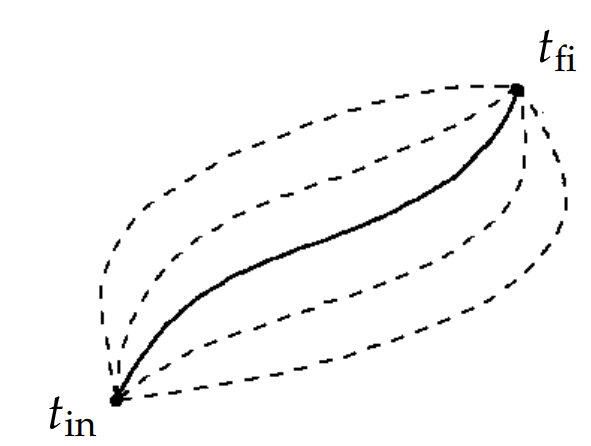
\includegraphics[scale=0.25]{Capitulos/Cap_2/minacc.png}
    \caption{Posibles caminos $q_{i}(t)$ que puede seguir un sistema en el espacio de las coordenadas
entre un instante inicial $t_{1}$ y otro final $t_{2}$.}
    \label{mA}
\end{figure}

Para ver lo que esto implica, considere variaciones infinitesimales alrededor de una trayectoria definida por $q_{i}(\mathbf{r},t)$ y $\dot{q}_{i}(\mathbf{r},t)$,

\begin{eqnarray}
q_{i}(\mathbf{r},t) &\rightarrow &q_{i}(\mathbf{r},t)+\delta q_{i}(\mathbf{r},t)  \label{2.2} \\
\dot{q}_{i}(\mathbf{r},t) &\rightarrow &\dot{q}_{i}(\mathbf{r},t)+\delta 
\dot{q}_{i}(\mathbf{r},t)~~~~~.  \label{2.2a}
\end{eqnarray}

Esto introduce la siguiente variaci\'{o}n de la acci\'{o}n definida en la
ecuaci\'{o}n (\ref{2.1}),

\begin{eqnarray}
\delta S &=&\delta \int_{t_{1}}^{t_{2}}dt\ L\left( q_{i},\dot{q}%
_{i},t\right) =\int_{t_{1}}^{t_{2}}dt\ \left( \frac{\partial L}{\partial
q_{i}}\delta q_{i}+\frac{\partial L}{\partial \dot{q}_{i}}\delta \dot{q}%
_{i}\right)   \notag \\
&=&\int_{t_{1}}^{t_{2}}dt\ \left( \frac{\partial L}{\partial q_{i}}\delta
q_{i}+\frac{\partial L}{\partial \dot{q}_{i}} \frac{d}{dt}\delta q_{i} \right)
,  \label{2.3}
\end{eqnarray}
aquí se ha considerado que:
\begin{equation}
\delta \dot{q}_{i}=\frac{\partial \dot{q}_{i}}{\partial \alpha} \delta \alpha=\frac{\partial}{\partial \alpha}\left(\frac{\mathrm{d} q_{i}}{\mathrm{~d} t}\right) \delta \alpha=\frac{\mathrm{d}}{\mathrm{d} t}\left(\frac{\partial q_{i}}{\partial \alpha}\right) \delta \alpha=\frac{\mathrm{d}}{\mathrm{d} t} \delta q_{i}~,
\end{equation}
siendo $\alpha$ un conjunto discreto de parámetros tal que $q_{i}= q_{i}(\alpha,t)$ es lo suficientemente suave de modo que las derivadas respecto a $\alpha$ y respecto a $t$ conmutan, de modo que es posible discretizar ambas variaciones. También se ha utilizado la convenci\'{o}n de suma para el \'{\i}ndice $i$. Suponiendo que el sistema es conservativo, el lagrangiano que describe el sistema no tiene ninguna dependencia temporal expl\'{\i}cita. Entonces al integrar por partes resulta,

\begin{equation}
\delta S=\left. \frac{\partial L}{\partial \dot{q}_{i}}\delta
q_{i}\right\vert _{t_{1}}^{t_{2}}+\int_{t_{1}}^{t_{2}}dt\ \left[ \frac{%
\partial L}{\partial q_{i}}-\frac{d}{dt}\left( \frac{\partial L}{\partial 
\dot{q}_{i}}\right) \right] \delta q_{i}  \label{2.3a}.
\end{equation}

\begin{exercise}
Demostrar aplicando integraci\'{o}n por partes, que se cumple la relaci\'{o}%
n (\ref{2.3a})
\end{exercise}

\begin{solution}
Para llegar a la expresi\'{o}n (\ref{2.3a}), se considera la integral 
\begin{equation}
\int_{t_{1}}^{t_{2}}dt\ \frac{\partial L}{\partial \dot{q}_{i}} \frac{d}{dt} \delta q_{i}  \label{2.3b}
\end{equation}%
aplicando integraci\'{o}n por partes $\int_{a}^{b}udv=\left. uv\right\vert
_{a}^{b}-\int_{a}^{b}vdu$, entonces se requiere definir 
\begin{equation*}
u=\frac{\partial L}{\partial \dot{q}_{i}}~\ \ \ \ ,~~~dv=dt\ \frac{d}{dt} \delta q_{i} \quad \ ,~~\ \ du=\frac{d}{dt}\left( \frac{\partial L}{\partial 
\dot{q}_{i}}\right) dt~.
\end{equation*}%
de aqu\'{\i} se obtiene 
\begin{equation*}
v=\int dt\ \frac{d\left( \delta
q_{i}\right) }{dt}=\delta q_{i}~~\impliedby \text{Variaciones sobre las
coordenadas y no sobre $t$}
\end{equation*}%
de manera que en (\ref{2.3b}),
\begin{equation}
\int_{t_{1}}^{t_{2}}dt\ \frac{\partial L}{\partial \dot{q}_{i}} \frac{d}{dt}\delta q_{i}=\left. \left( \frac{\partial L}{\partial \dot{q}_{i}}\delta
q_{i}\right) \right\vert _{t_{1}}^{t_{2}}-\int_{t_{1}}^{t_{2}}dt\ \delta
q_{i}\frac{d}{dt}\left( \frac{\partial L}{\partial \dot{q}_{i}}\right).
\label{2.3c}
\end{equation}%

Reemplazando (\ref{2.3c}) en la integral (\ref{2.3}):%
\begin{eqnarray}
\delta S &=&\int_{t_{1}}^{t_{2}}dt\ \frac{\partial L}{\partial q_{i}}\delta
q_{i}+\int_{t_{1}}^{t_{2}}dt\frac{\partial L}{\partial \dot{q}_{i}}\frac{d}{dt}\delta q_{i} \notag\label{2.4a} \\
&=&\int_{t_{1}}^{t_{2}}dt\ \frac{\partial L}{\partial q_{i}}\delta
q_{i}+\left. \frac{\partial L}{\partial \dot{q}_{i}}\delta q_{i}\right\vert
_{t_{1}}^{t_{2}}-\int_{t_{1}}^{t_{2}}dt\ \delta q_{i}\frac{d}{dt}\left( 
\frac{\partial L}{\partial \dot{q}_{i}}\right)   \notag \\
&\therefore &~\delta S=\left. \frac{\partial L}{\partial \dot{q}_{i}}\delta
q_{i}\right\vert _{t_{1}}^{t_{2}}+\int_{t_{1}}^{t_{2}}dt\ \left[ \frac{%
\partial L}{\partial q_{i}}-\frac{d}{dt}\left( \frac{\partial L}{\partial 
\dot{q}_{i}}\right) \right] \delta q_{i}~.  \label{2.4}
\end{eqnarray}

\end{solution}

Dado que se están buscando caminos que conectan las configuraciones inicial y final $q_{i}(t_{1})$ y $q_{i}(t_{2})$, no se variar\'{a}n los puntos
finales. As\'{\i}, entonces se establece que los puntos extremos estén fijos de manera que
\begin{equation}
\delta q_{i}(t_{1})=\delta q_{i}(t_{2})=0~,  \label{2.5}
\end{equation}

conllevando a que el primer t\'{e}rmino de la ecuaci\'{o}n (\ref{2.4}) desaparezca. El principio de m\'{\i}nima acci\'{o}n establece que, cerca del camino cl\'{a}sico, la variaci\'{o}n de la acci\'{o}n debe ser cero. Esto es cierto para cualquier variaci\'{o}n virtual arbitraria, es decir, para 
cualquier $\delta q_{i}(t)$, entonces, $\delta S=0$ ocurre si,

\begin{equation}
\frac{\partial L}{\partial q_{i}}-\frac{d}{dt}\left( \frac{\partial L}{%
\partial \dot{q}_{i}}\right) =0~, ~~~~~~~~\text{(Ecuaciones de Euler-Lagrange)}   \label{2.6}
\end{equation}

\vspace{0.1cm}
donde se ha puesto de manifiesto el teorema fundamental del calculo variacional. A (\ref{2.6}) se las conoce en la literatura como las
ecuaciones de movimiento de Euler-Lagrange, correspondientes a las coordenadas $q_{i}$.\\


\begin{exercise}
Encontrar la ecuaci\'{o}n de movimiento descrita por una part\'{\i}cula de
masa $m$ que se mueve bajo la influencia de un potencial $V\left( x\right) $
independiente del tiempo.\\
\end{exercise}
\begin{solution}
Para una part\'{\i}cula de masa $m$ que se mueve en un potencial $V(x)$
independiente del tiempo, una opci\'{o}n conveniente y que usualmente se usa
para el lagrangiano es:%
\begin{equation*}
L=T-V
\end{equation*}%
\begin{equation}
L=\frac{1}{2}m\dot{x}^{2}-V\left( x\right) ~.  \label{2.7}
\end{equation}%
Entonces la ecuaci\'{o}n de Euler-Lagrange derivada de este lagrangiano es:%
\begin{equation*}
\frac{\partial L}{\partial x}=\frac{dV\left( x\right) }{dx}~\ \ \ \ ;~\ \ \
\ \frac{\partial L}{\partial \dot{x}}=m\dot{x}
\end{equation*}%
\begin{equation*}
\frac{d}{dt}\left( \frac{\partial L}{\partial \dot{q}_{i}}\right) =m\ddot{x}~,
\end{equation*}%
de ahi que en (\ref{2.6}) se obtenga%
\begin{equation}
m\ddot{x}=\frac{dV\left( x\right) }{dx}~,  \label{2.8}
\end{equation}%
que se conoce com\'{u}nmente como \emph{la segunda ley de Newton} de
movimiento.
\end{solution}

\subsection{Formalismo Hamiltoniano y corchetes de Poisson}

La parte independiente de la velocidad del Lagrangiano se puede considerar
como energ\'{\i}a potencial generalizada. As\'{\i} que, se puede hacer que
las ecuaciones de Euler-Lagrange se vean como la segunda ley de Newton
definiendo los \emph{momentos can\'{o}nicos conjugados} generalizados
asociados a la coordenada $q_{i}$\ como:

\begin{equation}
p_{i}=\frac{\partial L(q_{i},\dot{q}_{i})}{\partial \dot{q}_{i}}~.
\label{2.9}
\end{equation}

Habr\'{a} una de estas ecuaciones para cada valor del \'{\i}ndice $i$,
siempre y cuando el sistema a tratar sea regular. Dado que el Lagrangiano es
una funci\'{o}n de las posiciones y las velocidades, los lados derechos de
estas ecuaciones son, en general, funciones de las $q^{\prime }s$ y las $%
\dot{q}^{\prime }s$. Suponer que estas ecuaciones son invertibles, es decir,
las $\dot{q}^{\prime }s$ pueden resolverse en t\'{e}rminos de las posiciones
y los momentos, esto es posible siempre que el determinante de la matriz
Hessiana sea diferente de cero.

Entonces se introduce el Hamiltoniano escrito en t\'{e}rminos de las nuevas
variables $(q,p),$ el cual resulta de aplicar una transformaci\'{o}n de
Legendre al lagrangiano, de este modo:\bigskip 

\begin{equation}
H\left( q,p\right) =p_{i}\dot{q}_{i}\left( q,p\right) -L\left( q,\dot{q}%
\left( q,p\right) \right) ~.  \label{2.10}
\end{equation}

Sin embargo, por diferenciaci\'{o}n se tiene

\begin{eqnarray}
dH &=&p_{i}d\dot{q}_{i}+\dot{q}_{i}dp_{i}-dL\left( q,\dot{q}\right) 
\label{2.11} \\
&=&p_{i}d\dot{q}_{i}+\dot{q}_{i}dp_{i}-\left( \frac{\partial L}{\partial
q_{i}}dq_{i}+\frac{\partial L}{\partial \dot{q}_{i}}d\dot{q}_{i}\right)  
\notag \\
&=&p_{i}d\dot{q}_{i}+\dot{q}_{i}dp_{i}-\frac{\partial L}{\partial q_{i}}%
dq_{i}-p_{i}d\dot{q}_{i}~.  \label{2.11a}
\end{eqnarray}

Los t\'{e}rminos con $d\dot{q}_{i}$ se cancelan entre s\'{\i} debido a la definici\'{o}n de momento can\'{o}nico conjugado en la ecuaci\'{o}n (2.9). El t\'{e}rmino con $dq_{i}$ se puede simplificar mediante el uso de la ecuaci\'{o}n de Euler-Lagrange y la ecuaci\'{o}n (\ref{2.9}), para que finalmente se pueda escribir

\begin{eqnarray*}
p_{i} &=&\frac{\partial L(q_{i},\dot{q}_{i})}{\partial \dot{q}_{i}}~\ \implies ~\frac{d}{dt}p_{i}=\frac{d}{dt}\left[ \frac{\partial L(q_{i},\dot{q}_{i})}{\partial \dot{q}_{i}}\right] =\frac{\partial L}{\partial q_{i}} \\
&\therefore &~\ \dot{p}_{i}=\frac{\partial L}{\partial q_{i}}~,
\end{eqnarray*}

\bigskip de manera que en (\ref{2.11a}),

\begin{equation}
dH=\dot{q}_{i}dp_{i}-\dot{p}_{i}dq_{i}~.  \label{2.12}
\end{equation}%
confirmando el hecho de que el hamiltoniano es de hecho una funci\'{o}n de
las posiciones y los momentos. Adem\'{a}s, conduce directamente a las
ecuaciones de movimiento de Hamilton:

\begin{equation}
\dot{q}_{i}=\frac{\partial H}{\partial p_{i}}~\ \ \ ~\ ,\qquad \dot{p}_{i}=-%
\frac{\partial H}{\partial q_{i}}~.  \label{2.13}
\end{equation}

\bigskip

Por otro lado, el corchete de Poisson de dos variables din\'{a}micas
cualesquiera se define de la siguiente manera:

\begin{equation}
\left\{ f_{1},f_{2}\right\} =\frac{\partial f_{1}}{\partial q_{i}}\frac{%
\partial f_{2}}{\partial p_{i}}-\frac{\partial f_{1}}{\partial p_{i}}\frac{%
\partial f_{2}}{\partial q_{i}}~,  \label{2.14}
\end{equation}

\noindent
bajo esta definici\'{o}n, es trivial verificar que

\begin{eqnarray*}
\left\{ q_{i},p_{j}\right\}  &=&\frac{\partial q_{i}}{\partial q_{k}}\frac{%
\partial p_{j}}{\partial p_{k}}-\frac{\partial q_{i}}{\partial p_{k}}\frac{%
\partial p_{j}}{\partial q_{k}}=\delta _{ik}\delta _{jk} \\
&=&\delta _{ij}~,
\end{eqnarray*}

%es decir

%\begin{equation}
%\left\{ q_{i},p_{j}\right\} =\delta _{ij}~~~~~,  \label{2.15}
%\end{equation}

\noindent
y que las ecuaciones de Hamilton se pueden reescribir como:

\begin{equation}
\dot{q}_{i}=\left\{ q_{i},H\right\} \qquad~~;~~ \qquad \dot{p}_{i}=\left\{ p_{i},H\right\} _{p}~.  \label{2.16}
\end{equation}

M\'{a}s generalmente, si $f$ es una variable din\'{a}mica, su evoluci\'{o}n temporal se puede escribir en t\'{e}rminos el par\'{e}ntesis de Poisson como

\begin{equation}
\dot{f}\equiv \frac{df}{dt}=\frac{\partial f}{\partial t}+\left\{f,H\right\} ~,  \label{2.17}
\end{equation}

\noindent
donde $\frac{\partial f}{\partial t}$\ ocurre si $f$ tiene una dependencia temporal expl\'{\i}cita.

\section{Formalismo Lagrangiano en teoría Clásica de Campos}

\subsection{La funcional Acción y el Lagrangiano}

\vspace{0.2cm}
En principio, pasar a una teor\'{\i}a de campo es sencillo, para ello se considera ahora un sistema como un 
campo o un conjunto de campos, siendo un campo esencialmente \emph{un conjunto de n\'{u}meros en cada punto 
del espacio-tiempo.}\\

\noindent
Para describir este sistema se construye una acci\'{o}n de tal modo que esta se pueda escribir como la integral 
de tiempo de un lagrangiano, pero el tiempo no es la \'{u}nica variable independiente en este caso, tambi\'{e}n 
se tiene que incorporar la informaci\'{o}n de todos los puntos del espacio en la acci\'{o}n.\\

\noindent
La forma intuitiva de hacer esto es escribiendo el Lagrangiano como una integral espacial de alguna funci\'{o}n de los campo, esto propone la ventaja adicional de poner el espacio y el tiempo en pie de igualdad en la integral. El integrando tiene entonces las dimensiones de una \emph{densidad lagrangiana}, concepto que se introduce dentro de poco.\\

\noindent
Sin embargo, en las discusiones sobre teor\'{\i}a de campos, esto siempre se denomina lagrangiano, y la palabra ``densidad'' est\'{a} impl\'{\i}cita en aras de la brevedad. Siempre se usar\'{a} la palabra lagrangiano en este sentido a partir de ahora. Sin embargo, lo se denotar\'{a} con el s\'{\i}mbolo $\mathcal{L}$ . Si en alg\'{u}n momento, es necesario usar la palabra lagrangiano en el sentido que se usa en la mec\'{a}nica de part\'{\i}culas, se llamar\'{a} el lagrangiano total y se denotar\'{a} por $L$.\\

\noindent
Ahora, el lagrangiano es una funcional de los campos, que se denota en el presente texto por $\phi_{i}$. Aqu\'{\i}, los diferentes valores del \'{\i}ndice $i$ pueden denotar campos completamente independientes, o los diferentes miembros de un conjunto de campos que est\'{a}n relacionados por alguna simetr\'{\i}a interna, o tal vez los componentes de un campo que se transforma no trivialmente bajo transformaciones de Lorentz, por ejemplo, como un vector. En cualquier caso,
el campo o campos indicados por $\phi_{i}$ toman el papel de las coordenadas $q_{i}$ de la ecuación (\ref{2.1}).\\

\begin{equation}
    q_{i}(t) \rightarrow \phi_{i}(t,\mathbf{x}) \equiv \phi(x)~. 
\end{equation}
\noindent
Para ver de manera un poco formal la introducci\'{o}n al campo cont\'{\i}nuo
se considera un conjunto de masas acopladas por un resorte en una dimensi\'{o}n como se muestra en la figura (\ref{osciladores}).\\

%--------------------------------------------------------------------------------
%OSCILADORES
%--------------------------------------------------------------------------------

\begin{figure}[h!]
\centering
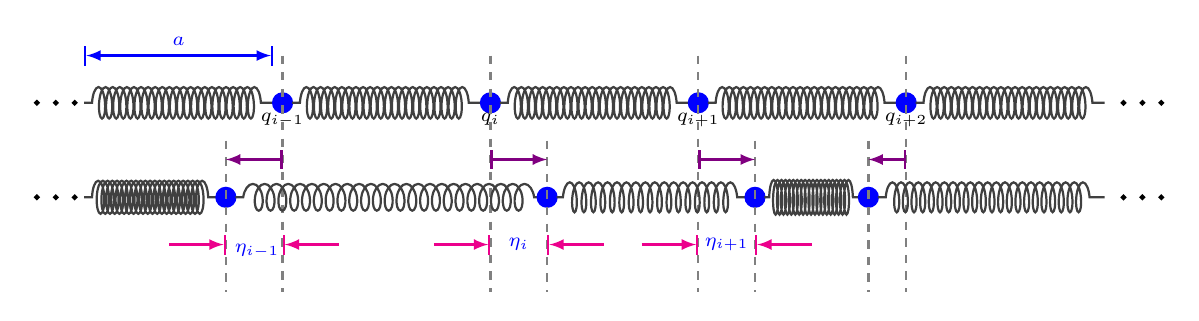
\begin{tikzpicture}[black!75,thick, scale=1.2]
\filldraw[black](-0.1,2)circle(0.5pt) node[below, black] {};
\filldraw[black](-0.3,2)circle(0.5pt) node[below, black] {};
\filldraw[black](-0.5,2)circle(0.5pt) node[below, black] {};
\draw[blue, |<->|, >=latex ](0,2.5) -- (2,2.5);
\node[above, blue] at (1,2.5){\scriptsize{$a$}};
\draw[decoration={coil, aspect=0.3, segment length=0.9mm, amplitude=2mm, pre length=1mm, post length=1mm}, decorate] (0,2) -- (2,2) node[midway,right=0.25cm,black]{}; 
\filldraw[blue](2.1,2)circle(1mm) node[below, black] {\scriptsize{$q_{i-1}$}};
\draw[dashed, gray](2.1,2.5)--(2.1,0);
\draw[decoration={coil, aspect=0.3, segment length=0.9mm, amplitude=2mm, pre length=1mm, post length=1mm}, decorate] (2.2,2) -- (4.2,2) node[midway,right=0.25cm,black]{}; 
\filldraw[blue](4.3,2)circle(1mm) node[below, black] {\scriptsize{$q_{i}$}};
\draw[dashed, gray](4.3,2.5)--(4.3,0);
\draw[decoration={coil, aspect=0.3, segment length=0.9mm, amplitude=2mm, pre length=1mm, post length=1mm}, decorate] (4.4,2) -- (6.4,2) node[midway,right=0.25cm,black]{}; 
\filldraw[blue](6.5,2)circle(1mm) node[below, black] {\scriptsize{$q_{i+1}$}};
\draw[dashed, gray](6.5,2.5)--(6.5,0);
\draw[decoration={coil, aspect=0.3, segment length=0.9mm, amplitude=2mm, pre length=1mm, post length=1mm}, decorate] (6.6,2) -- (8.6,2) node[midway,right=0.25cm,black]{}; 
\filldraw[blue](8.7,2)circle(1mm) node[below, black] {\scriptsize{$q_{i+2}$}};
\draw[dashed, gray](8.7,2.5)--(8.7,0);
\draw[decoration={coil, aspect=0.3, segment length=0.9mm, amplitude=2mm, pre length=1mm, post length=1mm}, decorate] (8.8,2) -- (10.8,2) node[midway,right=0.25cm,black]{}; 
\filldraw[black](11,2)circle(0.5pt) node[below, black] {};
\filldraw[black](11.2,2)circle(0.5pt) node[below, black] {};
\filldraw[black](11.4,2)circle(0.5pt) node[below, black] {};
%Resorte de Abajo
\filldraw[black](-0.1,1)circle(0.5pt) node[below, black] {};
\filldraw[black](-0.3,1)circle(0.5pt) node[below, black] {};
\filldraw[black](-0.5,1)circle(0.5pt) node[below, black] {};
\draw[decoration={coil, aspect=0.3, segment length=0.6mm, amplitude=2.1mm, pre length=1mm, post length=1mm}, decorate] (0,1) -- (1.4,1) node[midway,right=0.25cm,black]{}; 
\filldraw[blue](1.5,1)circle(1mm) node[below, black]{\scriptsize{}};
\draw[dashed, gray](1.5,1.6)--(1.5,0);
\draw[violet, <-|, >=latex ](1.5,1.4) -- (2.1,1.4);
\draw[magenta, ->|, >=latex ](0.9,0.5) -- (1.5,0.5);
\draw[magenta, |<-, >=latex ](2.1,0.5) -- (2.7,0.5);
\node[above, blue] at (1.83,0.25){\scriptsize{$\eta_{i-1}$}};
\draw[decoration={coil, aspect=0.5, segment length=1.5mm, amplitude=1.7mm, pre length=1mm, post length=0.8mm}, decorate] (1.6,1) -- (4.85,1) node[midway,right=0.25cm,black]{}; 
\filldraw[blue](4.9,1)circle(1mm) node[below, black] {\scriptsize{}};
\draw[dashed, gray](4.9,1.6)--(4.9,0);
\draw[violet, |->, >=latex ](4.3,1.4) -- (4.9,1.4);
\draw[magenta, ->|, >=latex ](3.7,0.5) -- (4.3,0.5);
\draw[magenta, |<-, >=latex ](4.9,0.5) -- (5.5,0.5);
\node[blue] at (4.6,0.5){\scriptsize{$\eta_{i}$}};
\draw[decoration={coil, aspect=0.3, segment length=1.2mm, amplitude=1.9mm, pre length=0.8mm, post length=0.5mm}, decorate] (5,1) -- (7,1) node[midway,right=0.25cm,black]{}; 
\filldraw[blue](7.1,1)circle(1mm) node[below, black]{\scriptsize{}};
\draw[dashed, gray](7.1,1.6)--(7.1,0);
\draw[violet, |->, >=latex ](6.5,1.4) -- (7.1,1.4);
\draw[magenta, ->|, >=latex ](5.9,0.5) -- (6.5,0.5);
\draw[magenta, |<-, >=latex ](7.1,0.5) -- (7.7,0.5);
\node[blue] at (6.8,0.5){\scriptsize{$\eta_{i+1}$}};
\draw[decoration={coil, aspect=0.2, segment length=0.5mm, amplitude=2.2mm, pre length=0.6mm, post length=0.5mm}, decorate] (7.2,1) -- (8.2,1) node[midway,right=0.25cm,black]{}; 
\filldraw[blue](8.3,1)circle(1mm) node[below, black]{\scriptsize{}};
\draw[dashed, gray](8.3,1.6)--(8.3,0);
\draw[violet, <-|, >=latex ](8.3,1.4) -- (8.7,1.4);
\draw[decoration={coil, aspect=0.3, segment length=1.1mm, amplitude=1.9mm, pre length=1mm, post length=1mm}, decorate] (8.4,1) -- (10.8,1) node[midway,right=0.25cm,black]{}; 
\filldraw[black](11,1)circle(0.5pt) node[below, black] {};
\filldraw[black](11.2,1)circle(0.5pt) node[below, black] {};
\filldraw[black](11.4,1)circle(0.5pt) node[below, black] {};
\end{tikzpicture} 
\caption{\emph{Sistema discreto de masas idénticas puntuales unidas por resortes con las mismas características.} \scriptsize{Fuente: Hecha en este proyecto}}
\label{osciladores}
\end{figure}

%--------------------------------------------------------------------------------------------------


\noindent
Utilizaremos como ejemplo ilustrativo, las vibraciones longitudinales de una varilla infinita. Se partir\'{a} entonces del sistema discreto que consiste en una cadena infinita de masas iguales espaciadas una distancia $a$, y conectadas a trav\'{e}s de resortes sin masa y uniformes (ver Fig.\ref{osciladores}), todos con la misma constante el\'{a}stica $k$.\\

\noindent
La infinitud de la cadena evita por el momento trabajar el problema de las condiciones de frontera (en los extremos). Se asumir\'{a} que las masas puntuales s\'{o}lo se pueden mover a lo largo de la cadena, en peque\~{n}as oscilaciones alrededor del punto de equilibrio. Denotando $\eta _{i}$ al desplazamiento de la $i$-esima part\'{\i}cula a partir de su posici\'{o}n de equilibrio, su energ\'{\i}a cin\'{e}tica es:

\begin{equation}
T=\frac{1}{2}\sum\limits_{i}m\dot{\eta}_{i}^{2}~,  \label{2.17a}
\end{equation}
\noindent
donde $m$ es la masa de cada part\'{\i}cula. La energ\'{\i}a potencial
correspondiente, resulta ser la suma de las energ\'{\i}as potenciales de
cada resorte, que surgen como resultado del estiramiento o compresi\'{o}n de
los mismos, as\'{\i}:

\begin{equation}
V=\frac{1}{2}\sum\limits_{i}k\left( \eta _{i+1}-\eta _{i}\right) ^{2}~.
\label{2.17b}
\end{equation}

\noindent
de manera que el lagrangiano que describe el sistemas es:

\begin{eqnarray}
L &=&T-V  \notag \\
&=&\sum\limits_{i}\left\{ \frac{1}{2}m\dot{\eta}_{i}^{2}-\frac{1}{2}k\left(
\eta _{i+1}-\eta _{i}\right) ^{2}\right\} ~,
\end{eqnarray}

\noindent
el cual puede ser escrito como:

\begin{eqnarray}
L &=&\frac{1}{2}\sum\limits_{i}a\left\{ \frac{m}{a}\dot{\eta}%
_{i}^{2}-ka\left( \frac{\eta _{i+1}-\eta _{i}}{a}\right) ^{2}\right\}  \notag
\\
&=&a\sum\limits_{i}L_{i}~,
\end{eqnarray}

\noindent
donde 
\begin{equation*}
L_{i}\equiv \frac{m}{a}\dot{\eta}_{i}^{2}-ka\left( \frac{\eta _{i+1}-\eta
_{i}}{a}\right) ^{2}~,
\end{equation*}

\noindent
y $a$ es la distancia entre los puntos del equilibrio.\\


Ahora se obtienen las ecuaciones de movimiento de Lagrange correspondientes
a las coordenadas $\eta _{i}$, de manera que se calcula:

\begin{eqnarray}
\frac{\partial L}{\partial \dot{\eta}_{k}} &=&\frac{1}{2}\sum\limits_{i}a%
\frac{\partial }{\partial \dot{\eta}_{k}}\left\{ \frac{m}{a}\dot{\eta}%
_{i}^{2}-ka\left( \frac{\eta _{i+1}-\eta _{i}}{a}\right) ^{2}\right\}  \notag
\\
&=&\sum\limits_{i}m\dot{\eta}_{i}\frac{\partial \dot{\eta}_{i}}{\partial 
\dot{\eta}_{k}}=\sum\limits_{i}m\dot{\eta}_{i}\delta _{ik}=m\dot{\eta}_{k}~,
\label{2.17d}
\end{eqnarray}

\begin{eqnarray}
\frac{\partial L}{\partial \eta _{k}} &=&\frac{1}{2}\sum\limits_{i}a\frac{%
\partial }{\partial \eta _{k}}\left\{ \frac{m}{a}\dot{\eta}_{i}^{2}-ka\left( 
\frac{\eta _{i+1}-\eta _{i}}{a}\right) ^{2}\right\} =-\frac{1}{2}%
\sum\limits_{i}\left\{ 2k\left( \eta _{i+1}-\eta _{i}\right) \frac{\partial
\left( \eta _{i+1}-\eta _{i}\right) }{\partial \eta _{k}}\right\}  \notag \\
&=&-\sum\limits_{i}k\left( \eta _{i+1}-\eta _{i}\right) \left[ \frac{%
\partial \eta _{i+1}}{\partial \eta _{k}}-\frac{\partial \eta _{i}}{\partial
\eta _{k}}\right] =-\sum\limits_{i}k\left( \eta _{i+1}-\eta _{i}\right) %
\left[ \delta _{i+1,k}-\delta _{ik}\right]  \notag \\
&=&-k\left[ \left( \eta _{k}-\eta _{k-1}\right) -\left( \eta _{k}-\eta
_{k+1}\right) \right] ~.  \label{2.17e}
\end{eqnarray}

\noindent
Entonces, al usar las ecuaciones de Lagrange para las coordenadas generalizadas $\eta _{k}$,
\begin{equation}
\frac{d}{dt}\left( \frac{\partial L}{\partial \dot{\eta}_{k}}\right) -\frac{%
\partial L}{\partial \eta _{k}}=0~,  \label{2.17c}
\end{equation}

\noindent
y empleando (\ref{2.17d}) con (\ref{2.17e}) se deriva

\begin{eqnarray}
m\ddot{\eta}_{i}-k\left[ \left( \eta _{i+1}-\eta _{i}\right) +\left(\eta_{i}-\eta _{i-1}\right) \right]=0~,  \label{2.17f}
\end{eqnarray}

\noindent 
donde se ha hecho el cambio de índice mudo $k \rightarrow i$. Dividiendo\ (\ref{2.17f}) entre $a$ implica:

\begin{equation}
\frac{m}{a}\ddot{\eta}_{i}-ka\frac{\left(\eta _{i+1}-\eta_{i}\right)}{a^{2}}+ka\frac{\left( \eta_{i}-\eta _{i-1}\right) }{a^{2}}=0~.
\label{2.17g}
\end{equation}
\noindent
Las anteriores ecuaciones se escogieron de esa forma con el fin de obtener una interpretaci\'{o}n sencilla de los par\'{a}metros en el l\'{\i}mite cuando $a\rightarrow 0$.\\
Es claro por ejemplo, que $m/a$ se reduce en el cont\'{\i}nuo a la densidad lineal de masa que se denota por $\mu$. No obstante, el l\'{\i}mite de $ka$ no es tan directo. Para una varilla el\'{a}stica que obedece la ley de Hooke, la elongaci\'{o}n de la varilla por unidad de longitud es proporcional a la fuerza o tensi\'{o}n ejercida a lo largo de \'{e}sta, lo cual se puede escribir como:

\begin{equation*}
F=Y\xi ~,
\end{equation*}

\noindent
donde $\xi $ es la enlongaci\'{o}n por unidad de longitud y $Y$ el modulo de Young. Por otro lado, la elongaci\'{o}n de un segmento $a$, por unidad de longitud del sistema discreto en cuesti\'{o}n, se escribe como:

\begin{equation*}
\xi =\frac{\eta _{i+1}-\eta _{i}}{a}~,
\end{equation*}
\noindent
la fuerza necesaria para estirar el resorte en esta cantidad es

\begin{equation}
F=k\left( \eta _{i+1}-\eta _{i}\right) =ka\left( \frac{\eta _{i+1}-\eta _{i}%
}{a}\right) ~,
\end{equation}

\noindent
indicando que $ka$ debe corresponder al m\'{o}dulo de Young $Y$ de la varilla cont\'{\i}nua. Al ir del sistema discreto al cont\'{\i}nuo, el \'{\i}ndice $i$, que identifica a una masa puntual espec\'{\i}fica, se convierte en una coordenada cont\'{\i}nua de posici\'{o}n $x$, de manera que en vez de la variable discreta $q_{i}$ ahora se tendr\'{\i}a una
variable de campo cont\'{\i}nua que para este problema es $\eta (x)$. Adicionalmente, la cantidad

\begin{equation}
\underset{a\rightarrow 0}{\lim }\frac{\eta _{i+1}-\eta _{i}}{a}=\underset{%
a\rightarrow 0}{\lim }\frac{\eta \left( x+a\right) -\eta \left( x\right) }{a}%
=\frac{d\eta }{dx}~,
\end{equation}
\noindent
se interpreta como una derivada de la variable de campo en relaci\'{o}n a una coordenada continua, de modo que $a$ hace el rol de $dx$.\\

\noindent
Finalmente, la suma sobre el \'{\i}ndice discreto $i$ se convierte en una integral sobre $x$ a lo largo de la longitud de la varilla. El Lagrangiano del sistema adquiere la forma

\begin{eqnarray}
L &=&\frac{1}{2}\sum\limits_{i}\left\{ a\frac{m}{a}\dot{\eta}_{i}^{2}-ka\left( \frac{\eta _{i+1}-\eta _{i}}{a}\right) ^{2}\right\}=\sum\limits_{i}aL_{i}~,~~~~~\text{(de lo discreto)}  \notag 
\end{eqnarray}
\noindent a
\begin{eqnarray}
L &=&\frac{1}{2}\int dx\ \left\{ \mu \dot{\eta}^{2}-Y\left( \frac{d\eta }{dx}\right) ^{2}\right\} \equiv \int dx  \mathcal{L}~.~~~~~\text{(En el continuo)}  \label{2.17h}
\end{eqnarray}

\vspace{0.3cm}
\noindent
Observe, que en el l\'{\i}mite cuando $a\rightarrow 0$, los \'{u}ltimos dos t\'{e}rminos de la ecuaci\'{o}n de movimiento (\ref{2.17g}) asociados a las coordenadas $\eta $ se convierten en:

\begin{eqnarray*}
ka\frac{\left(\eta _{i}-\eta _{i-1}\right) }{a^{2}}-ka\frac{\left(\eta_{i+1}-\eta_{i}\right) }{a^{2}}~\ &\implies &~\ \ Y\frac{\left( \eta_{i}-\eta_{i-1}\right) }{a^{2}}-Y\frac{\left( \eta _{i+1}-\eta_{i}\right) }{a^{2}}\qquad  \notag \\
\frac{Y}{a}\left[ \frac{\left( \eta_{i}-\eta _{i-1}\right) }{a}-\frac{\left( \eta_{i+1}-\eta_{i}\right) }{a}\right] ~\ &\implies &~\ \frac{Y}{a}\left[ \left( \frac{\eta \left( x\right) -\eta \left( x-a\right) }{a}\right)-\left( \frac{\eta \left( x+a\right) -\eta \left( x\right) }{a}\right)\right] ~,  \label{2.17i}
\end{eqnarray*}
\noindent
que en términos de derivadas se interpreta como siendo,
\begin{equation*}
\lim_{a\rightarrow 0}ka\left[ \left( \frac{\eta _{i}-\eta _{i-1}}{a^{2}}\right) -\left( \frac{\eta _{i+1}-\eta _{i}}{a^{2}}\right) \right] =\frac{Y}{a}\left[ \left( \frac{d\eta \left( x\right) }{dx}\right) _{x-a}-\left( \frac{d\eta}{dx}\right) _{x}\right]~.
\end{equation*}

\noindent
Al considerar nuevamente el l\'{\i}mite cuando $a\rightarrow 0$,

\begin{eqnarray}
\underset{a\rightarrow 0}{\lim }\frac{Y}{a}\left[ \left( \frac{d\eta (x)}{dx}\right) _{x-a}-\left( \frac{d\eta (x)}{dx}\right) _{x}\right] &=&-Y\underset{a\rightarrow 0}{\lim }\frac{1}{a}\left[ \left( \frac{d\eta (x)}{dx}\right)_{x}-\left( \frac{d\eta (x)}{dx}\right) _{x-a}\right]  \notag \\
&=&-Y\frac{d}{dx}\left( \frac{d\eta (x)}{dx}\right) \notag \\
&=&-Y\frac{d^{2}\eta (x)}{dx^{2}}~.  \label{2.17j}
\end{eqnarray}

\noindent
Por lo tanto, la extensi\'{o}n al cont\'{\i}nuo de la ecuaci\'{o}n de
movimiento (\ref{2.17g}) para la varilla el\'{a}stica es:

\begin{equation}
\frac{m}{a}\ddot{\eta}_{k}-ka\frac{\left( \eta _{k+1}-\eta _{k}\right) }{%
a^{2}}+ka\frac{\left( \eta _{k}-\eta _{k-1}\right) }{a^{2}}=0\ \implies ~\
\mu \frac{d^{2}\eta }{dt^{2}}-Y\frac{d^{2}\eta }{dx^{2}}=0~,
\label{2.17k}
\end{equation}

\noindent lo que se reescribe como
\begin{equation}
\frac{d^{2}\eta }{dt^{2}}=\frac{Y}{\mu }\frac{d^{2}\eta }{dx^{2}}~.
\label{Eonda}
\end{equation}

\noindent
La relaci\'{o}n (\ref{Eonda}) se conoce como ecuaci\'{o}n diferencial de onda unidimensional, para este caso longitudinal y que se propaga en un medio el\'{a}stico con velocidad:

\begin{equation*}
v=\sqrt{\frac{Y}{\mu}}~.
\end{equation*}

\vspace{1cm}
Este ejemplo sencillo ilustra la mayor parte de las caracter\'{\i}sticas generales que presenta el paso al cont\'{\i}nuo. Un aspecto muy relevante es el papel de la coordenada de posici\'{o}n $x$. Esta variable no representa una coordenada generalizada, es simplemente el \'{\i}ndice cont\'{\i}nuo que reemplaza al \'{\i}ndice $i$. As\'{\i}, como cada diferente valor de $i$ corresponde a una coordenada generalizada diferente $\eta _{i}$ del sistema discreto, de la misma forma hay una coordenada generalizada $\eta \left(x\right) $ por cada valor de $x$ en el sistema cont\'{\i}nuo. Dado que $\eta$ tambi\'{e}n es en general funci\'{o}n del par\'{a}metro cont\'{\i}nuo tiempo debemos escribir $\eta \left( x,t\right) $, esto indica que $x$ al igual que el tiempo se puede considerar como un par\'{a}metro que entra en el Lagrangiano y que estan rotulando al espacio y tiempo. Si el sistema cont\'{\i}nuo fuera tridimensional en lugar de unidimensional, las coordenadas generalizadas se rotular\'{\i}an con tres \'{\i}ndices cont\'{\i}nuos $x$, $y$, $z$ y las coordenadas generalizadas se escribir\'{\i}an como $\eta
(x,y,z,t)$.\\

\noindent
Vale la pena enfatizar que en la formulaci\'{o}n en el cont\'{\i}nuo, las cantidades $x$, $y$, $z$, $t$ son completamente independientes unas de otras, y solo aparecen como variables expl\'{\i}citas en $\eta$ en este caso. Por lo tanto, las derivadas de $\eta $ con respecto a cualquiera de ellas se pueden escribir como derivadas totales sin ninguna ambig\"{u}edad\footnote{Para evitar confusión con otros textos se las trabajara como derivadas parciales sabiendo que cada parámetro es independiente entre sí.}. Por otro lado la ecuaci\'{o}n asociada al lagrangiano (\ref{2.17h}) indica que este se escribe como una integral sobre el \'{\i}ndice cont\'{\i}nuo $x$, donde $\mathcal{L}$ caracteriza al integrando. Entonces en el correspondiente caso tridimensional el lagrangiano tendr\'{a} la forma:
\begin{equation}
L=\int d^{3}x\ \mathcal{L}~,  \label{2.17l}
\end{equation}

\noindent
siendo $\mathcal{L}$ la correspondiente \textbf{densidad lagrangiana}, que para una serie de vibraciones longitudinales en la varilla de acuerdo a (\ref{2.17h}), viene dada por:

\begin{equation}
\mathcal{L}=\frac{1}{2}\left[ \mu \dot{\eta}^{2}-Y\left( \frac{d\eta }{dx}\right) ^{2}\right] ~.  \label{2.17m}
\end{equation}

Antes de entrar en detalle con la teoría clásica de campos, se hará un breve repaso de la formulacón lagrangiana en una dimensión para sistemas continuos.

\vspace{1cm}
\subsection{Formulaci\'{o}n Lagrangiana en una dimensi\'{o}n para sistemas cont\'{\i}nuos}
\vspace{0.5cm}
De la ecuaci\'{o}n (\ref{2.17m}) se observa que la densidad lagrangiana asociada a la varilla el\'{a}stica depende de $\dot{\phi}\equiv \frac{\partial \phi }{\partial t}$ y $\frac{\partial \phi }{\partial x}$, donde se ha hecho el cambio de notación en el campo $\eta \rightarrow \phi$. Esto indica que $x$ y $t$ juegan un rol similar como par\'{a}metros de la densidad Lagrangiana.\\
Si hubiera fuerzas locales presentes adem\'{a}s de las interacciones entre vecinos, se puede tener una $\mathcal{L}$ que dependa de $\phi$ como tal, adem\'{a}s del gradiente espacial de $\phi$ y su derivada
temporal. En el caso m\'{a}s general la densidad lagrangiana puede ser tambi\'{e}n funci\'{o}n expl\'{\i}cita de $x$ y $t$ como es el caso de un campo externo que no sea constante ni uniforme. Entonces, la densidad Lagrangiana
para un sistema cont\'{\i}nuo unidimensional aparece como una funci\'{o}n de la variable de campo $\phi$ en la forma:

\begin{equation}
\mathcal{L}=\mathcal{L}\left(\phi ,\frac{\partial \phi }{\partial t},\frac{\partial \phi }{\partial x}x,t\right) ~,  \label{2.17n}
\end{equation}

\noindent
siendo el lagrangiano total $L$, la integral de la densidad $\mathcal{L}$ sobre todo el
rango de valores de $x$ que define al sistema.\\

\noindent
\begin{cabox}
Al extender el formalismo Lagrangiano a sistemas continuos, es claro que dicho sistema será identificado por los campos $\phi(x,t)$ los cuales toman un valor en cada punto del espacio y también por una densidad lagrangiana. Por lo tanto, los campos son ahora los grados de libertad que caracterizan al sistema físico y junto con sus derivadas deberán describir completamente la dinámica del sistema.\\

\noindent
Ahora, dado al interés de estudiar teorías relativistas, esta densidad lagrangiana deberá ser \emph{invariante bajo transformaciones de Lorentz}, es decir deberá ser un escalar, lo que va asegurar que las ecuaciones de campo sean coovariantes bajo estas transformaciones.\\
\end{cabox}

\noindent
Generalmente, para construir una densidad lagrangiana se considerarán polinomios en los campos y en sus derivadas aún cuando también existen modelos con términos no polinomiales los cuales se han y están estudiando. Otra característica de $\mathcal{L}$ es que sea una cantidad real, ya que hasta el momento ningún sistema clásico que se conozca sugiere una densidad compleja.\\

\noindent
La práctica ha demostrado que la densidad lagrangiana que describirá un sistema físico se puede escoger tan simple como sea posible, dado que una cantidad $\mathcal{L}$ , las expresiones $\mathcal{L}^{n}$ o alguna función de $\mathcal{L}$ son también invariantes por transformaciones de Lorentz. Así, se consideran las formas mas simples de funciones de los campos y sus derivadas los cuales serán suficientes para que su validez sea confirmada por los resultados experimentales, por esta razón se tendrá presente que la densidad Lagrangiana dependa en cada punto del espacio-tiempo, del valor del campo y sus derivadas evaluadas en dicho punto (o  en una vecindad del mismo). Cuando ocurre esto, se dice que la teoría es local.\\
Teorías donde el valor de un campo en un punto dependerá del valor del mismo campo evaluado en otro punto se llaman no locales; aún cuando estas teorías son concebibles, son demasiado complejas.\\


Para ser un poco más generales, e irnos familiarizarnos con la notación, la teoría que estamos considerando es de un solo campo $\phi=\phi(x,t)$ donde $(x,t)$ representa un punto en el espacio-tiempo unidimensional, entonces la densidad lagrangiana (\ref{2.17n}) se reescribirá como:

\begin{equation}
    \mathcal{L}=\mathcal{L}(\phi,\partial_{0}\phi,\partial_{1}\phi)~,
\end{equation}

\noindent
donde hemos introducido la notación de relatividad especial:
\begin{equation*}
    \partial_{0}\phi \equiv \frac{\partial \phi}{\partial t}~~~~~,~~~~~\partial_{1}\phi \equiv \frac{\partial \phi}{\partial x}~.
\end{equation*}


Con el fin de encontrar las ecuaciones de movimiento asociadas a dicho lagrangiano, se construye la acción asociada al sistema físico, la cual debe ser invariante por transformaciones de Lorentz, así:

\begin{equation}
    S[\phi]=\int_{t_{1}}^{t_{2}} \int_{x_{1}}^{x_{2}} dt dx \mathcal{L}(\phi,\partial_{0}\phi,\partial_{1}\phi)~,
\end{equation}

\noindent
la cual es una funcional de los campos. Cabe resaltar, que esta cantidad contendrá mas información sobre el sistema físico que la misma densidad Lagrangiana, dado que ella permitirá deducir las ecuaciones de campo. Su definición como una integral abarca la región del espacio tiempo donde el sistema físico esta definido, así $S$ hace una descripción global del sistema.\\

Ahora, se procederá a obtener las ecuaciones de campo generalizando el principio de Hamilton de la mecánica clásica según el cual la acción debe ser un mínimo para los estados actuales del sistema, es decir, $S$ deberá ser un mínimo para aquellas funciones $\phi$ que son soluciones de las ecuaciones de campo,

\begin{equation}
    \delta S[\phi]=\delta \int_{t_{1}}^{t_{2}} \int_{x_{1}}^{x_{2}} dt dx \mathcal{L}(\phi,\partial_{0}\phi,\partial_{1}\phi)=0~,  \label{2.17o}
\end{equation}


\noindent
indicando que las ecuaciones de movimiento deben obtenerse haciendo una variaci\'{o}n de la integral asociada a $\mathcal{L}$. El procedimiento es muy similar al caso discreto, la variaci\'{o}n se hace solo sobre $\phi$ y sus derivadas; los par\'{a}metros $x$, $t$ no se ven afectados por la variaci\'{o}n o trav\'{e}s de los l\'{\i}mites de integrac\'{o}n.\\

\noindent
Además, en analogía con la mecánica clásica la variaci\'{o}n de $\phi$ se tomará nula en los extremos temporales $t_{1}$ y $t_{2}$, y en los extremos espaciales $x_{1}$, $x_{2}$ de la integraci\'{o}n en $x$, en otras palabras se tiene condici\'{o}n de extremo fijo en los par\'{a}metros.\\

\noindent
De igual manera que en el principio variacional de Hamilton discreto se considera una familia de caminos variados introducidos muy convenientemente, en el espacio de las $\phi$ ocurre los mismo, donde $\phi$ se escoge a partir de una familia uniparam\'{e}trica de las posibles funciones,

\begin{equation*}
\phi \left( x,t,\alpha \right) =\phi \left( x,t,0\right) +\alpha \zeta \left( x,t\right)~,
\end{equation*}

\noindent
siendo $\alpha$ el parámetro que caracteriza cada camino y $\zeta \left(x,t\right)$ cualquier funci\'{o}n bien comportada que se anula en los puntos extremos de $x$ y $t$. La característica que se impone es que $\phi (x,t,0)$ denote la funci\'{o}n correcta que satisface el principio de Hamilton,\\

\noindent
Si $S$ se considera una funci\'{o}n de $\alpha$, de tal modo que tenga un extremo en $\phi (x,t,0)$ la derivada de $S$ con respecto a $\alpha $ se anula en $\alpha =0$ dado que esa es la trayectoria real que seguir\'{a} el sistema. Con base en esto y a trav\'{e}s de la diferenciaci\'{o}n directa se obtiene:

\begin{eqnarray}
\frac{dS}{d\alpha } &=&\frac{d}{d\alpha }\int_{t_{1}}^{t_{2}}\int_{x_{1}}^{x_{2}}dtdx\mathcal{L}=\int_{t_{1}}^{t_{2}}\int_{x_{1}}^{x_{2}}dtdx\frac{\partial \mathcal{L}}{\partial \alpha } \notag \\
&=&\int_{t_{1}}^{t_{2}}\int_{x_{1}}^{x_{2}}dtdx\left[ \frac{\partial \mathcal{L}}{\partial \phi }\frac{\partial \phi }{\partial \alpha }+\frac{\partial \mathcal{L}}{\partial \left( \partial _{0}\phi \right) }\frac{\partial \left( \partial _{0}\phi \right) }{\partial \alpha }+\frac{\partial \mathcal{L}}{\partial \left( \partial _{1}\phi \right) }\frac{\partial \left( \partial _{1}\phi \right) }{\partial \alpha }\right] ~,
\label{2.17p}
\end{eqnarray}

\noindent
sin embargo, puede ocurrir el hecho que $\mathcal{L}$ dependa expl\'{\i}citamente de $x$ y $t$, pero estos t\'{e}rminos no aparecen en la derivada anterior en virtud de que $\partial x/\partial \alpha =\partial t/\partial \alpha =0$, debido a que los par\'{a}metros no cambian cuando se hace una variaci\'{o}n del campo $\phi (x,t)$. Ahora bien, debido a que la variaci\'{o}n de $\phi$ representada por $\alpha \zeta \left( x,t\right) $, se anula en los extremos de ambos par\'{a}metros, una integraci\'{o}n por partes en $x$
y $t$ genera las relaciones:

\begin{equation}
\int_{t_{1}}^{t_{2}}dt\frac{\partial \mathcal{L}}{\partial \left( \partial_{0}\phi \right) }\frac{\partial \left( \partial _{0}\phi \right) }{\partial \alpha }=-\int_{t_{1}}^{t_{2}}dt\frac{d}{dt}\left[ \frac{\partial \mathcal{L}}{\partial \left( \partial _{0}\phi \right) }\right] \frac{\partial \phi }{\partial \alpha }~,
\label{2.17q}
\end{equation}

y

\begin{equation}
\int_{x_{1}}^{x_{2}}dx\frac{\partial \mathcal{L}}{\partial \left( \partial_{1}\phi \right) }\frac{\partial \left( \partial _{1}\phi \right) }{\partial \alpha }=-\int_{x_{1}}^{x_{2}}dx\frac{d}{dx}\left[ \frac{\partial \mathcal{L}}{\partial \left( \partial _{1}\phi \right) }\right] \frac{\partial \phi }{\partial \alpha }~.
\label{2.17r}
\end{equation}

Con estos resultados, la ecuación (\ref{2.17p}) se escribe,

\begin{equation*}
\frac{dS}{d\alpha }=\int_{t_{1}}^{t_{2}}\int_{x_{1}}^{x_{2}}dt\ dx\ \zeta \left( x,t\right) \left\{ \frac{\partial \mathcal{L}}{\partial \phi }-\frac{d}{dt}\left[ \frac{\partial \mathcal{L}}{\partial \left( \partial _{0}\phi \right) }\right] -\frac{d}{dx}\left[ \frac{\partial \mathcal{L}}{\partial \left( \partial _{1}\phi \right) }\right] \right\} =0~,
\end{equation*}

\noindent
y dado que $\zeta(x,t)$ es una función arbitraria entonces el término entre llaves debe anularse, por lo tanto

\begin{equation}
\boxed{
\frac{\partial \mathcal{L}}{\partial \phi }-\frac{d}{dt}\left[ \frac{\partial \mathcal{L}}{\partial \left( \partial _{0}\phi \right) }\right]-\frac{d}{dx}\left[ \frac{\partial \mathcal{L}}{\partial \left( \partial_{1}\phi \right) }\right] =0~,  \label{2.17s}
}
\end{equation}

\noindent
así se obtiene lo que se conoce como las ecuaciones de Euler Lagrange, determinadas a partir del principio de Hamilton\ (\ref{2.17o})\ llevado al limite cont\'{\i}nuo.\\


Un sistema de $n$ grados de libertad posee $n$ ecuaciones de Lagrange, sin embargo, \textexclamdown \emph{pareciera que para un sistema cont\'{\i}nuo solo se tuviera una ecuaci\'{o}n de Lagrange}!. Recuerde que en el caso discreto la ecuaci\'{o}n de movimiento para cada $\eta _{i}$ es una ecuaci\'{o}n diferencial que solo involucra al tiempo, en tal sentido la ultima ecuaci\'{o}n (\ref{2.17s}) nos da una ecuaci\'{o}n de movimiento para cada valor del \emph{\'{\i}ndice}\ cont\'{\i}nuo $x$. La naturaleza cont\'{\i}nua de $x$ se manifiesta en que la ecuaci\'{o}n (\ref{2.17s}) es una ecuaci\'{o}n diferencial parcial en $x$ y $t$, cuya soluci\'{o}n es de la forma $\phi \left( x,t\right) $. De lo anterior se desprende adem\'{a}s que la dimensi\'{o}n del espacio de configuraciones corresponde a la cardinalidad del espacio real (en una dos o tres dimensiones) ya que cada \'{\i}ndice cont\'{\i}nuo $x$ corresponde a un eje en el espacio de configuraciones.

\vspace{0.2cm}
\begin{exercise}
Usando integraci\'{o}n por partes, demostrar las relaciones (\ref{2.17q}) y (\ref{2.17r}).
\end{exercise}

\begin{solution}
Para mostrar (\ref{2.17q}) se utiliza la integral 

\begin{equation}
\int_{t_{1}}^{t_{2}}dt\ \frac{\partial \mathcal{L}}{\partial \left( \partial_{0}\phi \right) }\frac{\partial \left( \partial _{0}\phi \right) }{\partial \alpha }~,  \label{2.17ea}
\end{equation}

\noindent
al aplicar integraci\'{o}n por partes, se cumple $\int_{a}^{b}udv=\left. uv\right\vert _{a}^{b}-\int_{a}^{b}vdu$. Al definir 

\begin{equation*}
u\equiv \frac{\partial \mathcal{L}}{\partial \left( \partial _{0}\phi
\right) }~\ \ ~\ ,~\ \ \ \ dv=\frac{\partial \left( \partial _{0}\phi
\right) }{\partial \alpha }~dt\ ~\ \implies ~\ ~\ du\equiv \frac{d}{dt}%
\left( \frac{\partial \mathcal{L}}{\partial \left( \partial _{0}\phi \right) 
}\right) ~\ \ ~\ ,~\ \ \ \ v=\frac{\partial \phi }{\partial \alpha }~,
\label{2.17eb}
\end{equation*}

\noindent
y reemplazando en (\ref{2.17ea}), 
\begin{eqnarray*}
\int_{t_{1}}^{t_{2}}dt\ \frac{\partial \mathcal{L}}{\partial \left( \partial_{0}\phi \right) }\frac{\partial \left( \partial _{0}\phi \right)}{\partial \alpha } &=&\left. \frac{\partial \mathcal{L}}{\partial \left( \partial_{0}\phi \right) }\frac{\partial \phi }{\partial \alpha }\right\vert_{t_{1}}^{t_{2}}-\int_{t_{1}}^{t_{2}}dt\ \frac{d}{dt}\left[ \frac{\partial \mathcal{L}}{\partial \left( \partial _{0}\phi \right) }\right] \frac{\partial \phi }{\partial \alpha } \\
&=&\underset{0}{\underbrace{\left. \frac{\partial \mathcal{L}}{\partial \left( \partial _{0}\phi \right) }\zeta \left( x,t\right) \right\vert_{t_{1}}^{t_{2}}}}-\int_{t_{1}}^{t_{2}}dt\ \frac{d}{dt}\left[ \frac{\partial \mathcal{L}}{\partial \left( \partial _{0}\phi \right) }\right] \frac{\partial \phi }{\partial \alpha }~\ ,
\end{eqnarray*}
\begin{equation}
\therefore ~\ \ \int_{t_{1}}^{t_{2}}dt\ \frac{\partial \mathcal{L}}{\partial
\left( \partial _{0}\phi \right) }\frac{\partial \left( \partial _{0}\phi
\right) }{\partial \alpha }=-\int_{t_{1}}^{t_{2}}dt\ \frac{d}{dt}\left[ 
\frac{\partial \mathcal{L}}{\partial \left( \partial _{0}\phi \right) }%
\right] \frac{\partial \phi }{\partial \alpha }~.  \label{2.17ec}
\end{equation}

\noindent
Por otro lado, para demostrar la ecuaci\'{o}n (\ref{2.17r}), se debe aplicar integraci\'{o}n por partes a la expresi\'{o}n: 
\begin{equation*}
\int_{x_{1}}^{x_{2}}dx\ \frac{\partial \mathcal{L}}{\partial \left( \partial
_{1}\phi \right) }\frac{\partial \left( \partial _{1}\phi \right) }{\partial
\alpha }~,
\end{equation*}

\noindent
pero al compararla con (\ref{2.17ea}), se diferencian \'{u}nicamente en el
cambio del par\'{a}metro $t$ a $x$. Entonces, 
\begin{equation}
\int_{x_{1}}^{x_{2}}dx\ \frac{\partial \mathcal{L}}{\partial \left( \partial
_{1}\phi \right) }\frac{\partial \left( \partial _{1}\phi \right) }{\partial
\alpha }=-\int_{x_{1}}^{x_{2}}dx\ \frac{d}{dx}\left[ \frac{\partial \mathcal{%
L}}{\partial \left( \partial _{1}\phi \right) }\right] \frac{\partial \phi }{%
\partial \alpha }~.  \label{2.17ed}
\end{equation}
\end{solution}

\subsection{Formulaci\'{o}n Lagrangiana en tres dimensiones para sistemas cont\'{\i}nuos con un n\'{u}mero arbitrario de variables de campo}
\vspace{0.2cm}
\subsection*{\textcolor{orange}{Teoría clásica de campos}}
\vspace{0.3cm}
La formulaci\'{o}n Lagrangiana desarrollada aqu\'{\i} debe ser extendida a situaciones en dos y tres dimensiones, como es el caso por ejemplo de un s\'{o}lido  el\'{a}stico tridimensional. Adicionalmente, en lugar de un solo campo $\phi$ se podr\'{\i}a tener varias de estas cantidades. A manera de ejemplo, en tres dimensiones un desplazamiento arbitrario con respecto a la posici\'{o}n de equilibrio se describir\'{\i}a por un vector espacial de campo $\vb{\phi}$ con tres componentes, en la formulaci\'{o}n de Lagrange esto implica tres campos ya que las coordenadas generalizadas deben ser escalares.\\

\noindent
La extensi\'{o}n a m\'{a}s dimensiones o m\'{a}s campos no presenta dificultades significativas. Sin embargo, la notaci\'{o}n se vuelve altamente engorrosa cuando pasamos por ejemplo a tres dimensiones. Se puede notar sin embargo que el principio de Hamilton (\ref{2.17o}) y las ecuaciones de Euler Lagrange (\ref{2.17s}) anteriormente preescritas presentan una alta simetr\'{\i}a con respecto a las variables de espacio y
tiempo, las variables espaciales junto con el tiempo parecen cumplir el mismo rol, siendo los campos funciones tanto de las coordenadas espaciales como del tiempo, donde todas ellas deben ser tratadas como variables independientes. No hay por ejemplo, variaci\'{o}n de los campos en los l\'{\i}mites de integraci\'{o}n en el principio de Hamilton tanto sobre el espacio como sobre el tiempo. Debe tenerse en cuenta sin embargo, que aunque en esta formulaci\'{o}n las coordenadas espaciales y temporales entran en forma m\'{a}s sim\'{e}trica,
el tiempo NO corresponde a un \'{\i}ndice para la coordenada generalizada $\phi (\mathbf{x},t)$, esto se puede ver del hecho de que en el sistema discreto el campo $\eta _{i}(t)$ est\'{a} rotulado por el \'{\i}ndice $i$ pero no por la variable temporal, la cual simplemente mide la evoluci\'{o}n de una coordenada generalizada espec\'{\i}fica $\eta _{i}$.\\

\noindent
En consecuencia de lo anterior, es conveniente trabajar con una notaci\'{o}n en t\'{e}rminos de un espacio de cuatro dimensiones con coordenadas $x^{0}=t $, $x^{1}=x$, $x^{2}=y$, $x^{3}=z$ (En unidades naturales). Esta notaci\'{o}n no tiene ning\'{u}n significado f\'{\i}sico adicional\footnote{Al no trabajar en unidades naturales, el factor $c$ en $x^{0}$ es la velocidad de la luz en el vac\'{\i}o y es usada s\'{o}lo con el fin de que $x^{0}$ tenga las mismas unidades que $x^{i}$.}. El tensor m\'{e}trico $g$ es el correspondiente a una geometr\'{\i}a euclidiana, donde las transformaciones del grupo de Galileo son las transformaciones de coordenadas permitidas sobre las componentes del espacio con el tensor m\'{e}trico restringido por $g_{ij}=\delta_{ij}$. Nuevamente se retomar\'{a} la convenci\'{o}n de suma sobre \'{\i}ndices repetidos, donde las variables de campo se rotular\'{a}n con el sub\'{\i}ndice $r$, donde $r$ contará el número de campos necesarios para estudiar el problema\footnote{En algunas ocasiones simbolizar\'{a} un \'{\i}ndice simple de dos, tres, cuatro o m\'{a}s valores, pero tambi\'{e}n puede simbolizar un conjunto de m\'{u}ltiples \'{\i}ndices. Por ejemplo, si la variable de campo es un tensor espacial de segundo rango, entonces $r$ realmente se refiere a dos sub\'{\i}ndices.}.\\

\noindent
Finalmente, una derivada de las variables de campo con respecto a cualquiera de las cuatro coordenadas $x^{\mu}$ se denotar\'{a} como:

\begin{equation*}
\partial _{\nu }\phi _{r}=\phi_{r,\nu }=\frac{\partial \phi _{r}}{\partial x^{\nu }}~\ ~\ \ ,\qquad \partial _{j}\phi =\phi _{,j}=\frac{\partial \phi }{\partial x^{j}}~\ \ \ ~,\qquad \partial _{\mu}\partial_{\nu }\phi _{i}=\phi_{i,\mu \nu }=\frac{\partial ^{2}\phi_{i}}{\partial x^{\mu }\partial x^{\nu }}~.
\end{equation*}

\noindent
S\'{o}lo las derivadas de las variables de campos ser\'{a}n simbolizadas de
esta manera. En esta notaci\'{o}n la densidad Lagrangiana asociada al sistema se expresará en la siguiente forma,

\begin{equation}
\mathcal{L}=\mathcal{L}\left( \phi_{r}(x),\partial_{\mu}\phi_{r}(x),x\right)~.  \label{2.17t}
\end{equation}
donde $x\equiv (x^{\nu})$ identificará un punto en el espacio-tiempo, $\phi_{r}=\left\{\phi_{1}(x),\phi_{2}(x),\ldots \right\}$ el conjunto de campos que describen el problema y $\partial_{\mu}\phi_{r} \equiv \left\{\partial_{\mu}\phi_{1}(x),\partial_{\mu}\phi_{2}(x),\ldots \right\}$.\\

\noindent
El Lagrangiano total en analogía con una dimensión, se interpreta como una integral sobre el espacio tridimensional de la forma

\begin{eqnarray}
L &=&\int d^{3}x\ \mathcal{L}\left( \phi_{r},\partial _{\mu }\phi_{r},x\right)~, \qquad ~~~d^{3}x\equiv dx^{1}dx^{2}dx^{3}~,  \label{2.17u}
\end{eqnarray}

\noindent
de tal manera que la acción asociada al sistema físico sea una funcional de los campos definida como,
\begin{equation}
    S[\phi]=\int d^{4}x \mathcal{L}\left( \phi _{r},\partial _{\mu }\phi_{r},x\right)~, \qquad ~~~d^{4}x\equiv dx^{0}dx^{1}dx^{2}dx^{3}~,
\end{equation}

\noindent
siendo su definición como una integral que abarca aquellas regiones del espacio-tiempo donde el sistema físico está definido.\\

\noindent
Para determinar las ecuaciones de campo, como se mostró anteriormente se generaliza el principio del Hamilton de la mecánica clásica, es decir $S$ deberá ser un mínimo para aquellas funciones $\phi(x)$ que son soluciones de
\begin{equation}
    \delta S[\phi(x)]=0~,
\end{equation}

\noindent
lo que se conoce como el principio de mínima acción el cual escrito como una integral en el espacio-tiempo es de la forma:

\begin{eqnarray}
\delta S[\phi] &=&\delta \int d^{4}x\ \mathcal{L}\left( \phi _{r},\partial _{\mu
}\phi_{r},x\right)=0~.  \label{2.18}
\end{eqnarray}

\noindent
Al construir la variación de la acción, los extremos que en este caso serán las fronteras se deben mantener fijos, es decir los campos deben permanecer constantes en el infinito, por lo tanto:

\begin{itemize}
    \item La variación de los campos en los extremos $t_{1}$ y $t_{2}$ debe ser nula.
    \begin{equation*}
        \delta\phi(\mathbf{x},t_{1})=\delta\phi(\mathbf{x},t_{2})=0~.
    \end{equation*}
    \item Los campos deberán tener un comportamiento asintótico en el infinito\footnote{Se puede interpretar como que la variaci\'{o}n de $\phi_{r}$ sea nula al evaluarla sobre la hipersuperficie  $\Sigma$ que delimita a la regi\'{o}n de integraci\'{o}n en el espacio y el tiempo.}, es decir que cuando $\left\vert \mathbf{x}\right\vert \rightarrow \infty $, se debe cumplir que $\phi(x,t)\rightarrow0$. 
\end{itemize}
\vspace{0.4cm}
\noindent
Aplicando estas consideraciones a la variación en la acción
\begin{equation}
\delta S\left[ \phi \right] =\int d^{4}x\left[ \frac{\partial \mathcal{L}}{\partial \phi _{r}}\delta \phi _{r}+\frac{\partial \mathcal{L}}{\partial \left( \partial _{\mu }\phi _{r}\right) }\delta \left( \partial _{\mu }\phi_{r}\right) \right] ~,
\label{2aa}
\end{equation}
el segundo término se reduce a:
\begin{equation*}
\int d^{4}x\frac{\partial \mathcal{L}}{\partial \left( \partial _{\mu }\phi_{r}\right) }\delta \left( \partial _{\mu }\phi _{r}\right) =\int d^{4}x~\partial _{\mu }\left[ \frac{\partial \mathcal{L}}{\partial \left( \partial _{\mu }\phi _{r}\right) }\delta \phi _{r}\right] -\int d^{4}x~\partial _{\mu }\left[ \frac{\partial \mathcal{L}}{\partial \left( \partial _{\mu }\phi _{r}\right) }\right] \delta \phi _{r}~,
\end{equation*}
\noindent
donde el primer término de la linea anterior se anula, dado que al extender el \emph{teorema de Stokes} a un espacio de 4 dimensiones se tiene:
\begin{equation}
\int_{V}d^{4}x~\partial _{\mu }\left[ \frac{\partial \mathcal{L}}{\partial
\left( \partial _{\mu }\phi _{r}\right) }\delta \phi _{r}\right]
=\oint_{\Sigma }da~n_{\mu }\left[ \frac{\partial \mathcal{L}}{\partial \left(
\partial _{\mu }\phi _{r}\right) }\delta \phi _{r}\right]~, 
\end{equation}
siendo $n^{\mu}$ el vector normal a la superficie. Por lo tanto la condición de contorno exige que
\begin{equation*}
\left. \frac{{}}{{}}\delta \phi_{r} \right\vert _{\Sigma }=0~.
\end{equation*}

\noindent
Así que la expresión (\ref{2aa}) se reduce a 
\begin{eqnarray}
\delta S\left[ \phi \right]  &=&\int d^{4}x\left[ \frac{\partial \mathcal{L}%
}{\partial \phi _{r}}\delta \phi _{r}-\partial _{\mu }\left( \frac{\partial 
\mathcal{L}}{\partial \left( \partial _{\mu }\phi _{r}\right) }\right)
\delta \phi _{r}\right] \notag \\
&=&\int d^{4}x\left[ \frac{\partial \mathcal{L}}{\partial \phi _{r}}%
-\partial _{\mu }\left( \frac{\partial \mathcal{L}}{\partial \left( \partial
_{\mu }\phi _{r}\right) }\right) \right] \delta \phi _{r}=0~. \label{2ab}
\end{eqnarray}
\noindent
El hecho que la variación que se realiza en los campos $\delta \phi_{r}$ es completamente arbitraria, la condición que deberá ser garantizada para poder satisfacer la identidad (\ref{2ab}), según el lema fundamental del cálculo de variaciones, es que:
\begin{equation}
\boxed{
\frac{\partial \mathcal{L}}{\partial \phi _{r}}-\partial _{\mu }\left( \frac{%
\partial \mathcal{L}}{\partial \left( \partial _{\mu }\phi _{r}\right) }%
\right), \quad\quad r=1,2,3,\ldots 
\label{elagrange}
}
\end{equation}
estas expresiones son conocidas como las ecuaciones de Euler-Lagrange y corresponden a las ecuaciones de campo descrito por $\phi_{r}\equiv \left\{\phi_{1}(x),\phi_{2}(x),\ldots\right\}$, de tal modo que estas soluciones tornarán estacionaria a la acción.

%En el apéndice \ref{Apendice B} se tiene otra manera de deducir las ecuaciones de Euler-Lagrange para sistemas continuos, la cuál se realiza con analogía en la mecánica clásica.\\

\noindent
Es sencillo ver que las ecuaciones (\ref{elagrange}) se reducen a el caso unidimensional (es decir con un s\'{o}lo par\'{a}metro espacial $x$), con una sola variable de campo (i.e. $r=1$). Comparando las dos ecuaciones se puede apreciar la ventaja de la notaci\'{o}n introducida (y a\'{u}n m\'{a}s si se introducen las tres dimensiones).\\

\noindent
En sistemas discretos, el Lagrangiano tiene un grado de arbitrariedad ya que se puede adicionar una derivada total en el tiempo de una funci\'{o}n arbitraria de las coordenadas generalizadas y el tiempo sin alterar las ecuaciones de movimiento. Con sistemas cont\'{\i}nuos, la densidad Lagrangiana posee una simetr\'{\i}a gauge similar bajo la adici\'{o}n de un t\'{e}rmino de la forma:

\begin{equation}
\mathcal{L}^{\prime }=\mathcal{L}+\partial _{\mu }F_{\mu}(\phi_{r},x)~,  \label{2.23}
\end{equation}

%recordando de nuevo que la derivada total en $x$ es equivalente a una
%derivada parcial, se puede escribir el segundo t\'{e}rmino en la forma:

%\begin{equation*}
%\frac{dF_{\mu} \left(\phi_{r},x\right)}{dx^{\mu }}=\frac{\partial F_{\mu}\left(\phi_{r},x\right)}{\partial x^{\mu }}=\partial _{\mu }F_{\mu}~.
%\end{equation*}

\noindent
siendo el último t\'{e}rmino la extensi\'{o}n del operador divergencia en 4 dimensiones. $F_{\mu}$ son cuatro funciones arbitrarias de las variables de campo $\phi_{r}$ y las coordenadas $x$. La aplicaci\'{o}n del teorema de la divergencia en el espacio de 4 dimensiones convierte la integral de hipervolumen en una integral sobre la hipersuperficie $\Sigma^{\mu }$ donde la variaci\'{o}n de $F_{\mu }$ es nula.

\begin{equation}
\delta \int d^{4}x\left[ \frac{{}}{{}}\partial _{\mu }F_{\mu }\left( \phi
_{r},x\right) \right] =\delta \oint_{\Sigma }ds^{\mu }F_{\mu }\left( \phi
_{r},x\right) =0~.
\end{equation}

\noindent
Esto significa que el segundo t\'{e}rmino a la derecha en (\ref{2.23}) no contribuye a la variaci\'{o}n de la acci\'{o}n y por tanto, tampoco contribuye a las ecuaciones de movimiento. Además, indica que la expresi\'{o}n (\ref{2.23}) es una transformaci\'{o}n gauge para la densidad Lagrangiana y representa una extensi\'{o}n natural del gauge visto en mec\'{a}nica anal\'{\i}tica para el caso discreto, con las asignaciones $q_{i}(t)\rightarrow \phi _{r}\left( x^{\mu }\right) $ , $\ L\rightarrow \mathcal{L}$, $F\rightarrow F_{\mu }$, $\ t\rightarrow x$. La \'{u}ltima asignaci\'{o}n tiene que ver con el hecho de que el problema discreto es uniparam\'{e}trico (s\'{o}lo el tiempo es un par\'{a}metro) y el problema en el cont\'{\i}nuo es multiparam\'{e}trico (con par\'{a}metros $t$, $x^{i}$).

\bigskip

\begin{exercise}
Estudiar el segundo término de la ecuación (\ref{2aa}).
\end{exercise}

\begin{solution}
La ecuaci\'{o}n (\ref{2aa}) representa una variaci\'{o}n en la acci\'{o}n,

\begin{equation*}
\delta S\left[ \phi \right] =\int d^{4}x\left[ \frac{\partial \mathcal{L}}{%
\partial \phi _{r}}\delta \phi _{r}+\frac{\partial \mathcal{L}}{\partial
\left( \partial _{\mu }\phi _{r}\right) }\delta \left( \partial _{\mu }\phi
_{r}\right) \right] ~,
\end{equation*}

analizando el segundo t\'{e}rmino de la relaci\'{o}n anterior:

\begin{eqnarray*}
\int d^{4}x\frac{\partial \mathcal{L}}{\partial \left( \partial _{\mu }\phi_{r}\right) }\delta \left( \partial _{\mu }\phi _{r}\right)  &=&\int d^{4}x\left[ \frac{\partial \mathcal{L}}{\partial \left( \partial _{0}\phi_{r}\right) }\delta \left( \partial _{0}\phi _{r}\right) +\frac{\partial \mathcal{L}}{\partial \left( \partial _{i}\phi _{r}\right) }\delta \left(\partial _{i}\phi _{r}\right) \right]  \\
&=&\int d^{4}x\left[ \frac{\partial \mathcal{L}}{\partial \left( \partial_{0}\phi _{r}\right) }\delta \left( \frac{\partial \phi _{r}}{\partial t} \right) +\frac{\partial \mathcal{L}}{\partial \left( \partial _{i}\phi_{r}\right) }\delta \left( \frac{\partial \phi _{r}}{\partial x^{i}}\right) \right] ,
\end{eqnarray*}

aqu\'{\i} se utiliza el hecho que la variaci\'{o}n $\delta \phi _{r}$ conmuta con las derivadas espaciales y temporales por el hecho de que esta cambia la forma del campo y no el punto espacio-temporal donde esta esta siendo evaluada, se tiene que

\begin{eqnarray}
\int d^{4}x\frac{\partial \mathcal{L}}{\partial \left( \partial _{\mu }\phi
_{r}\right) }\delta \left( \partial _{\mu }\phi _{r}\right)  &=&\int d^{4}x%
\left[ \frac{\partial \mathcal{L}}{\partial \left( \partial _{0}\phi
_{r}\right) }\partial _{0}\delta \phi _{r}+\frac{\partial \mathcal{L}}{%
\partial \left( \partial _{i}\phi _{r}\right) }\partial _{i}\delta \phi _{r}%
\right]   \notag \\
&=&\int d^{4}x\frac{\partial \mathcal{L}}{\partial \left( \partial _{\mu
}\phi _{r}\right) }\partial _{\mu }\delta \phi _{r},
\end{eqnarray}

empleando la propiedad de la derivada de un producto (o su equivalente integraci\'{o}n por partes),

\begin{eqnarray}
\partial _{\mu }\left[ \frac{\partial \mathcal{L}}{\partial \left( \partial
_{\mu }\phi _{r}\right) }\delta \phi _{r}\right]  &=&\partial _{\mu }\left( 
\frac{\partial \mathcal{L}}{\partial \left( \partial _{\mu }\phi _{r}\right) 
}\right) \delta \phi _{r}+\frac{\partial \mathcal{L}}{\partial \left(
\partial _{\mu }\phi _{r}\right) }\partial _{\mu }\delta \phi _{r}  \notag \\
\frac{\partial \mathcal{L}}{\partial \left( \partial _{\mu }\phi _{r}\right) 
}\partial _{\mu }\delta \phi _{r} &=&\partial _{\mu }\left[ \frac{\partial 
\mathcal{L}}{\partial \left( \partial _{\mu }\phi _{r}\right) }\delta \phi
_{r}\right] -\partial _{\mu }\left( \frac{\partial \mathcal{L}}{\partial
\left( \partial _{\mu }\phi _{r}\right) }\right) \delta \phi _{r}~,
\end{eqnarray}%
se tiene que%
\begin{eqnarray*}
\int d^{4}x\frac{\partial \mathcal{L}}{\partial \left( \partial _{\mu }\phi
_{r}\right) }\delta \left( \partial _{\mu }\phi _{r}\right)  &=&\int d^{4}x%
\left[ \partial _{\mu }\left( \frac{\partial \mathcal{L}}{\partial \left(
\partial _{\mu }\phi _{r}\right) }\delta \phi _{r}\right) -\partial _{\mu
}\left( \frac{\partial \mathcal{L}}{\partial \left( \partial _{\mu }\phi
_{r}\right) }\right) \delta \phi _{r}\right]  \\
&=&\int d^{4}x\partial _{\mu }\left( \frac{\partial \mathcal{L}}{\partial
\left( \partial _{\mu }\phi _{r}\right) }\delta \phi _{r}\right) -\int
d^{4}x\partial _{\mu }\left( \frac{\partial \mathcal{L}}{\partial \left(
\partial _{\mu }\phi _{r}\right) }\right) \delta \phi _{r}~,
\end{eqnarray*}%
al estudiar la integral%
\begin{eqnarray*}
\int d^{4}x\partial _{\mu }\left( \frac{\partial \mathcal{L}}{\partial
\left( \partial _{\mu }\phi _{r}\right) }\delta \phi _{r}\right)  &=&\int
d^{4}x\left[ \partial _{0}\left( \frac{\partial \mathcal{L}}{\partial \left(
\partial _{0}\phi _{r}\right) }\delta \phi _{r}\right) +\partial _{i}\left( 
\frac{\partial \mathcal{L}}{\partial \left( \partial _{i}\phi _{r}\right) }%
\delta \phi _{r}\right) \right]  \\
&=&\int d^{4}x\partial _{0}\left( \frac{\partial \mathcal{L}}{\partial
\left( \partial _{0}\phi _{r}\right) }\delta \phi _{r}\right) +\int
d^{4}x\partial _{i}\left( \frac{\partial \mathcal{L}}{\partial \left(
\partial _{i}\phi _{r}\right) }\delta \phi _{r}\right)  \\
&=&\int_{V}d^{3}x\int_{t_{1}}^{t_{2}}dt~\partial _{0}\left( \frac{\partial 
\mathcal{L}}{\partial \left( \partial _{0}\phi _{r}\right) }\delta \phi
_{r}\right)\\
&+&\int_{t_{1}}^{t_{2}}dt\int_{V}d^{3}x~\partial _{i}\left( \frac{\partial \mathcal{L}}{\partial \left( \partial _{i}\phi _{r}\right) }\delta \phi _{r}\right) ~,
\end{eqnarray*}
efectuando cada integral, donde se aplica el teorema de Stokes al segundo t%
\'{e}rmino se deduce que,%
\begin{equation*}
\int d^{4}x\partial _{\mu }\left( \frac{\partial \mathcal{L}}{\partial
\left( \partial _{\mu }\phi _{r}\right) }\delta \phi _{r}\right)
=\int_{V}d^{3}x\left. \left( \frac{\partial \mathcal{L}}{\partial \left(
\partial _{0}\phi _{r}\right) }\delta \phi _{r}\right) \right\vert
_{t_{1}}^{t_{2}}+\int_{t_{1}}^{t_{2}}dt\oint_{S}dS_{i}\left( \frac{\partial 
\mathcal{L}}{\partial \left( \partial _{i}\phi _{r}\right) }\delta \phi
_{r}\right) ~,
\end{equation*}%
este resultado permite establecer que: la primera integral se anula por la
condici\'{o}n de frontera $\delta \phi _{r}\left( \mathbf{x},t_{1}\right)
=\delta \phi _{r}\left( \mathbf{x},t_{2}\right) =0$. De igual manera, en la
segunda integral el integrando esta siendo evaluado en la superficie que
encierra el volumen en el cual est\'{a}n siendo considerados los campos. Si
este volumen se extiende en todo el espacio, la superficie que lo limita
tiende a infinito y del comportamiento asint\'{o}tico de los campos hace que
esta integral de superficie tienda a cero. De esta manera, deducimos que 
\begin{equation*}
\int d^{4}x\partial _{\mu }\left( \frac{\partial \mathcal{L}}{\partial
\left( \partial _{\mu }\phi _{r}\right) }\delta \phi _{r}\right) =0~,
\end{equation*}%
por lo tanto,%
\begin{equation*}
\int d^{4}x\frac{\partial \mathcal{L}}{\partial \left( \partial _{\mu }\phi
_{r}\right) }\delta \left( \partial _{\mu }\phi _{r}\right) =\int d^{4}x%
\frac{\partial \mathcal{L}}{\partial \left( \partial _{\mu }\phi _{r}\right) 
}\partial _{\mu }\delta \phi _{r}=-\int d^{4}x\partial _{\mu }\left( \frac{%
\partial \mathcal{L}}{\partial \left( \partial _{\mu }\phi _{r}\right) }%
\right) \delta \phi _{r}~,
\end{equation*}%
determinando que la variaci\'{o}n de la acci\'{o}n se reescriba como
\begin{equation}
\delta S\left[ \phi \right] =\int d^{4}x\left[ \frac{\partial \mathcal{L}}{%
\partial \phi _{r}}\delta \phi _{r}-\partial _{\mu }\left( \frac{\partial 
\mathcal{L}}{\partial \left( \partial _{\mu }\phi _{r}\right) }\right)
\delta \phi _{r}\right] ~.
\end{equation}
\end{solution}

\section{Formalismo Hamiltoniano en teoría Clásica de Campos}
\vspace{0.2cm}

El formalismo Hamiltoniano se puede extender a teoría de campos mientras se mantenga una completa analogía con la mecánica clásica.\\

La superioridad de la formulación Hamiltoniana en relación a la Lagrangiana, radica en el hecho que la primera reposa en el hecho de que la teoría deberá ser invariante por transformaciones canónicas las cuales son mucho mas generales que las transformación de coordenadas en la que se basa la formulación Lagrangiana. Así, desde el punto de vista Hamiltoniana la equivalencia de dos sistemas físicos implica la existencia de una transformación canónica tomando coordenadas y momentos de un sistema en las coordenadas y momentos del otro.\\

Al trabajar en teoría de campos, se define el momento canónico conjugado del campo $\phi_{r}$ como siendo,

\begin{equation}
    \pi_r (x) \equiv \fdv{\lagdn}{\dot{\phi}_r} = \pdv{\lagdn}{\dot{\phi}_r}~.
\end{equation}

El sistema físico ahora se definirá en el espacio de fase $(\phi_{r},\pi_{r})$. El Hamiltoniano canónico en este espacio es definido por

\begin{equation}
    H = \int \dd[3]{x} \pi_{r}(x)\dot{\phi}_r (x)-L = \int \dd[3]{x} \qty\Big[\pi_{r}(x)\dot{\phi}_r (x)-\lagdn] \equiv \int \dd[3]{x} \mathcal{H}.
    \label{HC}
\end{equation}

Aquí aparece la \emph{densidad hamiltoniana canónica} que se escribe como

\begin{equation} \boxed{
    \mathcal{H} = \pi_{r} \dot{\phi}_r-\lagdn \qty(\phi,\partial_{\mu}\phi) =\pdv{\lagdn}{\dot{\phi}_r} \dot{\phi}_r-\lagdn \qty(\phi,\partial_{\mu}\phi) .}
    \label{dHC}
\end{equation}

Los paréntesis de Poisson (PP) asociados a dos variables dinámicas $F(x) \equiv F[\phi,\pi]$ y $G(x) \equiv G[\phi,\pi]$ (representan dos funcionales) a tiempos iguales se calcula como

\begin{equation}
    \{F(x), G(y)\} \equiv \{F(x), G(y)\}_{x^0=x^0} \equiv \int \dd[3]{z} \left[\frac{\delta F(x)}{\delta \phi_r(z)} \frac{\delta G(y)}{\delta \pi_r(z)}-\frac{\delta G(y)}{\delta \phi_r(z)} \frac{\delta F(x)}{\delta \pi_r(z)}\right]
\end{equation}

A partir de esta expresión, es posible observar que los PP fundamentales entre las variables fundamentales del espacio de fase $\left(\phi_r, \pi_r\right)$, que se consideran linealmente independientes, son:

\begin{IEEEeqnarray}{rCl}
    \left\{\phi_r(x), \pi_s(y)\right\} &=& \int \dd[3]{z} \qty\Bigg[\frac{\delta \phi_r(x)}{\delta \phi_k(z)} \frac{\delta \pi_s(y)}{\delta \pi_k(z)}-\cancelto{0}{\frac{\delta \pi_s(y)}{\delta \phi_k(z)}}\cancelto{0}{\frac{\delta \phi_r(x)}{\delta \pi_k(z)}}] \notag \\
    &=& \int \dd[3]{z} \delta_{r k} \delta^3(x-z) \delta_{s k} \delta^3(y-z) \notag \\
    &=& \delta_{rs} \delta^3(x-y).
\end{IEEEeqnarray}

De igual manera se determina que

\begin{IEEEeqnarray*}{rCl}
    \left\{\phi_r(x), \phi_s(y)\right\} &=& \int \dd[3]{z} \qty\Bigg[ \frac{\delta \phi_r(x)}{\delta \phi_k(z)} \cancelto{0}{\frac{\delta \phi_s(y)}{\delta \pi_k(z)}} - \frac{\delta \phi_s(y)}{\delta \phi_k(z)} \cancelto{0}{\frac{\delta \phi_r(x)}{\delta \pi_k(z)}}]=0. \\
    \left\{\pi_r(x), \pi_s(y)\right\} &=& \int \dd[3]{z} \qty\Bigg[ \cancelto{0}{\frac{\delta \pi_r(x)}{\delta \phi_k(z)}} \frac{\delta \pi_s(y)}{\delta \pi_k(z)}-\cancelto{0}{\frac{\delta \pi_s(y)}{\delta \phi_k(z)}}_0 \frac{\delta \pi_r(x)}{\delta \pi_k(z)}]=0.
\end{IEEEeqnarray*}

En analogía con la mecánica clásica, la evolución temporal de una observable $F(x) \equiv F[\phi, \pi]$ es dada por:

\begin{equation}
    \dot{F}(x)=\left\{F(x), H \right\}.
\end{equation}

A partir de esta expresión, es posible determinar las correspondientes ecuaciones de Hamilton son,

\begin{IEEEeqnarray}{rCl}
    \dot{\phi}_r(x)=\left\{\phi_r(x), H\right\}=\int \dd[3]{z} \frac{\delta \phi_r(x)}{\delta \phi_k(z)} \frac{\delta H}{\delta \pi_k(z)}=\frac{\delta H}{\delta \pi_r(x)} \\
    \dot{\pi}_r(x)=\left\{\pi_i(x), H \right\}=-\int \dd[3]{z} \frac{\delta H}{\delta \phi_k(z)} \frac{\delta \pi_r(x)}{\delta \pi_k(z)}=-\frac{\delta H}{\delta \phi_r(x)}.
\end{IEEEeqnarray}


\newpage
\section{Leyes de conservación en Teoría Clásica de Campos}
\vspace{0.2cm}

Un tema de interés en teoría clásica de campos es estudiar las propiedades de simetr\'{\i}a que presenta un Lagrangiano (o Hamiltoniano), hecho que implica la existencia de cantidades conservadas. Por tanto, si el Lagrangiano no contiene expl\'{\i}citamente una coordenada particular de desplazamiento, se conserva su momento can\'{o}nico conjugado correspondiente. La ausencia de la dependencia explícita de la coordenada significa que el lagrangiano no se ve afectado por una transformaci\'{o}n que altera el valor de esta, entonces se dice que dicho Lagrangiano es invariante o sim\'{e}trico bajo la transformaci\'{o}n dada.\\

De manera similar, la invariancia del Lagrangiano bajo el desplazamiento temporal implica la conservaci\'{o}n de la energ\'{\i}a. La relaci\'{o}n formal entre propiedades de simetr\'{\i}a (invariancia) y las cantidades conservadas est\'{a} contenida en el teorema de Noether. Es en el espacio de 4 dimensiones de la teor\'{\i}a cl\'{a}sica de campos donde el teorema alcanza su forma m\'{a}s sofisticada y f\'{e}rtil. Por esa raz\'{o}n, la discusi\'{o}n expl\'{\i}cita del teorema se ha reservado para el tratamiento de campos, aunque tambi\'{e}n se puede derivar una versi\'{o}n para sistemas discretos.

\subsection{Primer Teorema de Noether}  \label{seccion: Primer teorema de Noether}
\vspace{0.2cm}

El teorema de Noether implica discutir la relación existente entre \emph{simetrías continuas} y \emph{leyes de conservación} en teoría clásica de campos. Una simetría es una transformación de los campos que dejan invariante la acción, dichas simetrías pueden ser \emph{internas} si sólo \textbf{afectan al campo y no cambian las coordenadas} o \emph{espacio-temporales} en caso contrario. Por ejemplo, si tenemos un campo escalar sin masa, su Lagrangiano

\begin{equation}
    \mathcal{L}=\frac{1}{2}\partial_{\mu}\phi \partial^{\mu}\phi~,
\end{equation}
es invariante si hacemos la transformación $\phi \rightarrow \phi+\alpha$ con $\alpha$ constante. Este tipo de simetría es interna. Mientras que al cambiar $\phi(x)\rightarrow\phi(x+\alpha)$ también es una simetría pero espacio-temporal. Estas son simetrías continuas puesto que uno puede variar $\alpha$ de manera continua, en tanto que las simetrías discretas son por ejempo C, P y T.\\

\noindent
Puesto una transformaci\'{o}n continua se puede construir a partir de una superposici\'{o}n de transformaciones infinitesimales, la simetr\'{\i}a bajo una transformaci\'{o}n de coordenadas se escribe como

\begin{equation}
x^{\mu }\rightarrow x^{\prime \mu }=x^{\mu }+\delta x^{\mu }\left( x\right)
~,  \label{2.36}
\end{equation}
donde el cambio infinitesimal $\delta x^{\mu }$\ puede ser una funci\'{o}n de $x$. Como consecuencia de este cambio en las coordenadas, los campos $\phi _{r}\left( x\right) $ sufrir\'{a}n la siguiente transformaci\'{o}n

\begin{equation}
\phi _{r}^{\prime }\left( x^{\prime \mu }\right) =\phi _{r}\left( x^{\mu
}\right) +\delta \phi _{r}\left( x^{\mu }\right) ~,  
\end{equation}
\noindent
que por simplicidad de aquí en adelante se escribira como,
\begin{equation}
\phi _{r}^{\prime }\left( x^{\prime}\right) =\phi _{r}\left(x\right) +\delta \phi _{r}\left( x\right) ~,  \label{2.37}
\end{equation}
\noindent
siendo $\delta \phi _{r}\left( x\right) $ el efecto de los cambios en las coordenadas\ $x^{\mu }$ y en los campos $\phi _{r}$ la cual puede ser una funci\'{o}n de todas las dem\'{a}s cantidades de campo $\phi _{s}$. Además, de esta relación es posible deducir,
\begin{equation}
\delta \phi _{r}\left( x\right) =\phi _{r}^{\prime }\left( x^{\prime}\right)-\phi _{r}\left(x\right)~,  
\label{2.37_a}
\end{equation}
\noindent
relación conocida como \emph{varación local en los campos}, donde $x$ y $x^{\prime}$ hacen referencia al mismo punto en el espacio-tiempo pero representados en dos sistemas de referencia diferentes.\\

\noindent
Se define una \emph{variación total en los campos $\phi_{r}(x)$} como

\begin{equation}
\tilde{\delta}\phi _{r}\left( x\right) \equiv \phi _{r}^{\prime }\left( x\right) - \phi _{r}\left( x\right) ~,  \label{2.38}
\end{equation}
\noindent
el cual representa un cambio en una de las variables de campo (forma del campo) en un punto particular en el espacio-tiempo $x$. En otras palabras, $\bar{\delta}\phi _{r}\left( x^{\mu }\right) $ se la interpreta como una variación total en el campo donde se mantendrá fijo el valor de $x$ y solo cambiará la forma del campo $\phi_{r}$. Además, la descripci\'{o}n de las transformaciones en t\'{e}rminos de cambios infinitesimales de las cantidades no transformadas indica que estamos tratando solo con \emph{transformaciones continuas}. \footnote{La simetría bajo inversión en tres dimensiones (simetería de paridad) no es una de las simetrías a las que se puede aplicar el teorema de Noether.}

\noindent
Como consecuencia de las transformaciones tanto de las coordenadas (\ref{2.36}), como de las cantidades de campo (\ref{2.37}), la densidad Lagrangiana presentará la siguiente transformación infinitesimal,  

%el Lagrangiano aparece en general, como una funci\'{o}n diferente tanto de las variables de campo como de las coordenadas del espacio-tiempo,

%\begin{equation}
%\mathcal{L}\left( \phi _{r}\left( x\right) ,\partial _{\mu }\phi _{r}\left(
%x\right) \right) \rightarrow \mathcal{L}^{\prime }\left( \phi _{r}^{\prime
%}\left( x^{\prime }\right) ,\partial^{\prime}_{\mu }\phi _{r}^{\prime }\left(
%x^{\prime }\right) \right) ~,  \label{2.39}
%\end{equation}

%\noindent
%esto implica que $\mathcal{L}$ de acuerdo con (\ref{2.37}) presente la siguiente transformación infinitesimal,
\begin{equation}
\mathcal{L}^{\prime}\left(x^{\prime}\right) \equiv \mathcal{L}^{\prime} \left(\phi_{r}^{\prime}\left(x^{\prime}\right), \frac{\partial \phi_{r}^{\prime}\left(x^{\prime}\right)}{\partial x^{\prime}}\right)=\mathcal{L}\left(\phi_{r}(x), \frac{\partial \phi_{r}(x)}{\partial x}\right)+\delta \mathcal{L}(x)=\mathcal{L}(x)+\delta \mathcal{L}(x)~.
\label{2.39_a}
\end{equation}
Es importante enfatizar en el hecho que esta variación hace referencia a una transformación de coordenadas además de un cambio en la forma del campo.\\

\noindent
Sin embargo, se debe tener presente que \emph{el lagrangiano es una cantidad escalar al ser transformada de un sistema a otro}.\\

\noindent
La versi\'{o}n del teorema de Noether que presentaremos aqu\'{\i} no es la forma m\'{a}s general posible, pero es tal que facilita la derivaci\'{o}n sin restringir significativamente el alcance del teorema o la utilidad de las conclusiones. Se supondr\'{a} que se cumplen tres condiciones planteadas en la siguiente definición.

\vspace{1cm}
\begin{definition}
\label{definoether}
\textbf{Condiciones para derivar el teorema de Noether}
\begin{itemize}
\item[1.]  El espacio de 4 dimensiones es plano; es decir, es \textbf{euclidiano}, por ende se asume una m\'{e}trica plana donde se restringe el espacio-tiempo relativista al espacio de Minkowski, de manera que se trabaja con una m\'{e}trica plana.\\

\item[2.] La densidad lagrangiana muestra la misma forma funcional en t\'{e}rminos
de las cantidades transformadas que de las cantidades originales, es decir,%
\begin{equation}
\mathcal{L}^{\prime }\left( \phi _{r}^{\prime }\left( x^{\prime }\right)
,\partial _{\mu }\phi _{r}^{\prime }\left( x^{\prime }\right) \right) =
\mathcal{L}\left( \phi _{r}^{\prime }\left( x^{\prime }\right) ,\partial^{\prime}
_{\mu }\phi _{_{r}}^{\prime }\left( x^{\prime }\right) \right) ~,
\label{2.40}
\end{equation}
en otras palabras hacemos una transformaci\'{o}n en los campos garantizando que la forma funcional de la lagrangiana no cambie.\\

\item[3.] La magnitud de la integral de acci\'{o}n es invariante bajo la transformaci\'{o}n de coordenadas y campos, es decir,
\begin{equation}
S^{\prime }[\phi^{\prime}]\equiv \int_{\Omega ^{\prime }}d^{4}x^{\prime} \mathcal{L}^{\prime }\left(\phi _{r}^{\prime }\left( x^{\prime}\right),\partial^{\prime}_{\mu }\phi_{r}^{\prime }\left( x^{\prime }\right) ,x^{\prime }\right) =\int_{\Omega }d^{4}x \mathcal{L}\left( \phi_{r}\left( x\right) ,\partial _{\mu }\phi _{r}\left( x \right),x\right)=S[\phi] ~,  \label{2.41}
\end{equation}
Siendo $\Omega^{\prime}$ el mismo volumen de integración $\Omega$ pero expresado en las nuevas coordenadas $x^{\prime}$.\\

Esta condición garantiza que la transformación que estamos realizando es de \emph{simetría}, dejando invariante las ecuaciones de movimiento. 
%El elemento de volumen $d^{4}x$ es invariante y es definido en la región delimitada por $\Omega$. Por lo tanto $d^{4}x^{\prime}=d^{4}x$.
%En forma general se cumple que $d^{4}x^{\prime}=\sqrt{|g|}dx^{0}dx^{1}dx^{2}dx^{3}$ de tal modo que $\sqrt{|g|}=\sqrt{|\det \left( g\right) |}$ \emph{(valor absoluto de la ra\'{\i}z cuadrada del determinante de $g$)}.
\end{itemize}
\label{defiN}
\end{definition}

\vspace{0.5cm}
\noindent
Particularmente, en mecánica analítica no se hace hincapié en la condición \textbf{2.} en el estudio de cantidades conservadas de sistemas discretos, principalmente porque se ha satisfecho autom\'{a}ticamente bajo las transformaciones consideradas. Cuando se transforman coordenadas c\'{\i}clicas por desplazamiento, el cambio de origen implícito no altera la dependencia funcional que el Lagrangiano tiene a trav\'{e}s de las variables. Pero en los tipos m\'{a}s amplios de transformaci\'{o}n que se est\'{a}n tratando ahora se convierte en una propiedad de simetr\'{\i}a que requiere su estudio.\\

\noindent
Tenga presente que la ecuaci\'{o}n (\ref{2.40}) asegura que las ecuaciones de movimiento tienen la misma forma, ya sea que se expresen en t\'{e}rminos de las variables antiguas o nuevas, este hecho se denomina \emph{invariancia
de forma}. No obstante, la condici\'{o}n de invarianza de forma no es la circunstancia m\'{a}s general bajo la cual esto es cierto; las densidades lagrangianas original y transformada tambi\'{e}n pueden diferir por una cuadridivergencia sin modificar las ecuaciones de movimiento como se mencionó anteriormente\footnote{De hecho, es posible realizar la derivaci\'{o}n del teorema de Noether con una versi\'{o}n ampliada de la invarianza de forma dado que la integral de volumen de la cuadridivergencia desaparece en el infinito. Pero por simplicidad se limitar\'{a} a trabajar con la ecuaci\'{o}n (\ref{2.40}).}.\\

\noindent
Por otro lado, de la condici\'{o}n \textbf{3.} asociada a la ecuaci\'{o}n (\ref{2.41}), se tiene que la magnitud de la integral de acci\'{o}n es invariante bajo una transformación de coordenadas. Esto representa una ampliaci\'{o}n, que incluyen, propiedades anteriores de simetr\'{\i}a asociadas a las coordenadas c\'{\i}clicas. El lagrangiano no cambia num\'{e}ricamente bajo la traslaci\'{o}n de una coordenada c\'{\i}clica, ni el valor de la acci\'{o}n integral. Teniendo presente esto, se denominar\'{a} a (\ref{2.41}) \emph{condici\'{o}n de invariancia de escala}.\\

\noindent
As\'{\i} pues, las condiciones \textbf{2.} y \textbf{3.} representan generalizaciones de las condiciones de simetr\'{\i}a o invariancia que llevaron a la existencia de cantidades conservadas para sistemas discretos.\\

%-----------------------Material Greiner--------------------------------------------------------------------

\noindent
De la relación (\ref{2.38}), es posible establecer una conexión entre una variación total y una variación local a partir de una expansión en serie de potencias en $\delta x^{\mu}(x)$,

$$
\begin{aligned}
\phi_{r}^{\prime}\left(x^{\prime}\right) &=\phi_{r}^{\prime}(x+\delta x) \approx \phi_{r}^{\prime}(x)+\delta x^{\mu} \partial_{\mu} \phi_{r}^{\prime}(x) \\
&=\phi_{r}(x)+\tilde{\delta} \phi_{r}(x)+\delta x^{\mu} \partial_{\mu} \phi_{r}(x)+\delta x^{\mu} \partial_{\mu} \tilde{\delta} \phi_{r}(x) \\
& \approx \phi_{r}(x)+\tilde{\delta} \phi_{r}(x)+\delta x^{\mu} \partial_{\mu} \phi_{r}(x)
\end{aligned}
$$
donde se han mantenido aproximaciones hasta de primer orden. Utilizando la expresión (\ref{2.37_a}), la relación anterior es posible expresarla se la siguiente manera:

\begin{equation}
\delta \phi_{r}(x) \approx \tilde{\delta} \phi_{r}(x)+\delta x^{\mu} \partial_{\mu} \phi_{r}(x) ~.    
\label{2.38_aa}
\end{equation}
\noindent
Esta expresión se interpreta diciendo que la variación total en los campos se puede expresar como consecuencia de un cambio en la forma funcional de los mismos y debido a un cambio en las coordenadas.\\

\noindent
Una de las características que presenta la variación total es conmutar con el operador derivada, es decir:

\begin{equation}
\partial _{\mu }\tilde{\delta}\phi _{r}\left( x\right) =\partial _{\mu }\left(\phi _{r}^{\prime }\left( x\right) -\phi _{r}\left( x\right) \right)=\partial _{\mu }\phi _{r}^{\prime }\left( x\right) -\partial _{\mu }\phi_{r}\left( x\right) \equiv \tilde{\delta}\left( \partial _{\mu }\phi_{r}\left( x\right) \right) ~.  \label{eq2.42}
\end{equation}

\noindent
Sin embargo, la variación local no presenta esta característica dado que:
\begin{eqnarray*}
\partial _{\mu }\delta \phi _{r}\left( x\right)  &=&\partial _{\mu }\left(\phi _{r}^{\prime }\left( x^{\prime }\right) -\phi _{r}\left( x\right) \right)  \\
&=&\frac{\partial \phi _{r}^{\prime }\left( x^{\prime }\right) }{\partial x^{\mu }}-\frac{\partial \phi _{r}\left( x\right) }{\partial x^{\mu }} \\
&=&\underset{\delta \left[ \partial _{\mu }\phi _{r}\left( x\right) \right] }{\underbrace{\frac{\partial \phi _{r}^{\prime }\left( x^{\prime }\right) }{\partial x^{\prime \mu }}-\frac{\partial \phi _{r}\left( x\right) }{\partial x^{\mu }}}}+\frac{\partial \phi _{r}^{\prime }\left( x^{\prime }\right) }{\partial x^{\mu }}-\frac{\partial \phi _{r}^{\prime }\left( x^{\prime }\right) }{\partial x^{\prime \mu }} \\
&=&\delta \left[ \partial _{\mu }\phi _{r}\left( x\right) \right] +\frac{\partial \phi _{r}^{\prime }\left( x^{\prime }\right) }{\partial x^{\prime \nu }}\frac{\partial x^{\prime \nu }}{\partial x^{\mu }}-\frac{\partial \phi_{r}^{\prime }\left( x^{\prime }\right) }{\partial x^{\prime \mu }} \\
&=&\delta \left[ \partial _{\mu }\phi _{r}\left( x\right) \right] +\partial_{\nu }^{\prime }\phi _{r}^{\prime }\left( x^{\prime }\right) \frac{\partial }{\partial x^{\mu }}\left( x^{\nu }+\delta x^{\nu }\left( x\right) \right) -\partial _{\mu }^{\prime}\phi _{r}^{\prime }\left( x^{\prime }\right)  \\
&=&\delta \left[ \partial _{\mu }\phi _{r}\left( x\right) \right] +\partial_{\nu }^{\prime }\phi _{r}^{\prime }\left( x^{\prime }\right) \left( \frac{\partial x^{\nu }}{\partial x^{\mu }}+\frac{\partial }{\partial x^{\mu }} \delta x^{\nu }\left( x\right) \right) -\partial _{\mu }^{\prime}\phi _{r}^{\prime }\left( x^{\prime }\right)  \\
&=&\delta \left[ \partial _{\mu }\phi _{r}\left( x\right) \right] +\partial_{\nu }^{\prime }\phi _{r}^{\prime }\left( x^{\prime }\right) \left( \delta_{\mu }^{\nu }+\frac{\partial }{\partial x^{\mu }}\delta x^{\nu }\left(x\right) \right) -\partial _{\mu }^{\prime }\phi _{r}^{\prime }\left(x^{\prime }\right)  \\
&=&\delta \left[ \partial _{\mu }\phi _{r}\left( x\right) \right] +\partial_{\mu }^{\prime }\phi _{r}^{\prime }\left( x^{\prime }\right) +\partial_{\nu }^{\prime }\phi _{r}^{\prime }\left( x^{\prime }\right) \frac{\partial }{\partial x^{\mu }}\delta x^{\nu }\left( x\right) -\partial _{\mu }^{\prime}\phi _{r}^{\prime }\left( x^{\prime }\right) 
\end{eqnarray*}
obteniendo a primer orden que,
\begin{equation}
\partial _{\mu }\delta \phi _{r}\left( x\right) =\delta \left(\partial _{\mu }\phi _{r}\left( x\right) \right) +\partial _{\nu }^{\prime}\phi _{r}^{\prime }\left( x^{\prime }\right) \partial_{\mu}\delta x^{\nu }\left( x\right) ~.
\label{eq2.39}
\end{equation}

\noindent
No obstante, esta relación implica calcular las siguientes derivadas
\begin{eqnarray}
\partial _{\nu }^{\prime }\phi _{r}^{\prime }\left( x^{\prime }\right)  &=& \frac{\partial }{\partial x^{\prime \nu }}\left[ \phi _{r}\left( x\right) +\delta \phi _{r}\left( x\right) \right] =\frac{\partial }{\partial x^{\alpha }}\left[ \phi _{r}\left( x\right) +\delta \phi _{r}\left( x\right) \right] \frac{\partial x^{\alpha }}{\partial x^{\prime \nu }}  \notag \\
&=&\left[ \frac{\partial \phi _{r}\left( x\right) }{\partial x^{\alpha }}+\frac{\partial \delta \phi _{r}\left( x\right) }{\partial x^{\alpha }}\right]\frac{\partial x^{\alpha }}{\partial x^{\prime \nu }}  \notag \\
&=&\left[ \partial _{\alpha }\phi _{r}\left( x\right) +\partial _{\alpha}\delta \phi _{r}\left( x\right) \right] \frac{\partial x^{\alpha }}{\partial x^{\prime \nu }}~,
\label{eq2.40}
\end{eqnarray}

\noindent
y

\begin{eqnarray}
\frac{\partial x^{\alpha }}{\partial x^{\prime \nu }} &=&\frac{\partial }{\partial x^{\prime \nu }}\left[ x^{\prime \alpha }-\delta x^{\alpha }\left(x\right) \right] =\frac{\partial x^{\prime \alpha }}{\partial x^{\prime \nu }}-\frac{\partial }{\partial x^{\prime \nu }}\delta x^{\alpha }\left(x\right)   \notag \\
&=&\delta _{\nu }^{\alpha }-\frac{\partial }{\partial x^{\beta }}\delta x^{\alpha }\left( x\right) \frac{\partial x^{\beta }}{\partial x^{\prime \nu}}  \notag \\
&=&\delta _{\nu }^{\alpha }-\frac{\partial \left( \delta x^{\alpha }\left(x\right) \right) }{\partial x^{\beta }}\frac{\partial }{\partial x^{\prime \nu }}\left[ x^{\prime \beta }-\delta x^{\beta }\left( x\right) \right]  \notag \\
&=&\delta _{\nu }^{\alpha }-\partial _{\beta }\left( \delta x^{\alpha}\left( x\right) \right) \left[ \frac{\partial x^{\prime \beta }}{\partial x^{\prime \nu }}-\frac{\partial }{\partial x^{\prime \nu }}\delta x^{\beta}\left( x\right) \right]   \notag \\
&=&\delta _{\nu }^{\alpha }-\partial _{\beta }\left( \delta x^{\alpha }\left( x\right) \right) \left[ \delta _{\nu }^{\beta }-\frac{\partial \left( \delta x^{\beta }\left( x\right) \right) }{\partial x^{\prime \nu }}\right]   \notag \\
&=&\delta _{\nu }^{\alpha }-\partial _{\beta }\left( \delta x^{\alpha}\left( x\right) \right) \delta _{\nu }^{\beta }+\partial _{\beta }\left(\delta x^{\alpha }\left( x\right) \right) \partial _{\nu }^{\prime }\left(\delta x^{\beta }\left( x\right) \right)   \notag \\
&\approx &\delta _{\nu }^{\alpha }-\partial _{\nu }\left( \delta x^{\alpha}\left( x\right) \right) ~,
\label{eq2.41}
\end{eqnarray}

\noindent
demostrando en (\ref{eq2.40}) la relación a primer orden,
\begin{eqnarray*}
\partial _{\nu }^{\prime }\phi _{r}^{\prime }\left( x^{\prime }\right)  &=& \left[ \partial _{\alpha }\phi _{r}\left( x\right) +\partial _{\alpha }\delta \phi _{r}\left( x\right) \right] \left[ \delta _{\nu }^{\alpha}-\partial _{\nu }\left( \delta x^{\alpha }\left( x\right) \right) \right] \\
&=&\left[ \partial _{\alpha }\phi _{r}\left( x\right) +\partial _{\alpha}\delta \phi _{r}\left( x\right) \right] \delta _{\nu }^{\alpha }-\left[ \partial _{\alpha }\phi _{r}\left( x\right) +\partial _{\alpha }\delta \phi_{r}\left( x\right) \right] \partial _{\nu }\delta x^{\alpha }\left(x\right)  \\
&=&\partial _{\nu }\phi _{r}\left( x\right) +\partial _{\nu }\delta \phi_{r}\left( x\right) -\partial _{\alpha }\phi _{r}\left( x\right) \partial_{\nu }\delta x^{\alpha }\left( x\right) +\partial _{\alpha }\left( \delta \phi _{r}\left( x\right) \right) \partial _{\nu }\left( \delta x^{\alpha }\left( x\right) \right)  \\
&\approx &\partial _{\nu }\phi _{r}\left( x\right) +\partial _{\nu }\delta \phi _{r}\left( x\right) -\partial _{\alpha }\phi _{r}\left( x\right) \partial _{\nu }\delta x^{\alpha }\left( x\right) ~, 
\end{eqnarray*}

\noindent
de modo que en (\ref{eq2.39}) se deriva la expresión,

\begin{eqnarray}
\partial _{\mu }\delta \phi _{r}\left( x\right)  &=&\delta \left( \partial_{\mu }\phi _{r}\left( x\right) \right) +\left[ \partial _{\nu }\phi_{r}\left( x\right) +\partial _{\nu }\delta \phi _{r}\left( x\right)-\partial _{\alpha }\phi _{r}\left(x\right) \partial _{\nu }\delta x^{\alpha }\left( x\right) \right] \partial _{\mu }\delta x^{\nu }\left(x\right)   \notag \\
&\approx &~\delta \left( \partial _{\mu }\phi _{r}\left( x\right) \right)+\partial _{\nu }\phi _{r}\left( x\right) \partial _{\mu }\delta x^{\nu}\left( x\right) ~.
\label{eq2.43}
\end{eqnarray}

\noindent
En resumen, los resultados (\ref{eq2.42}) y (\ref{eq2.43}) establecen que,
\begin{eqnarray*}
\left( \partial _{\mu }\tilde{\delta}-\bar{\delta}\partial _{\mu }\right) \phi_{r}\left( x\right)  &\equiv &\left[ \partial _{\mu },\tilde{\delta}\right] \phi _{r}\left( x\right) =0~, \\
\left( \partial _{\mu }\delta -\delta \partial _{\mu }\right) \phi_{r}\left( x\right)  &\equiv &\left[ \partial _{\mu },\delta \right] \phi_{r}\left( x\right) =\partial _{\nu }\phi _{r}\left( x\right) \partial _{\mu}\delta x^{\nu }\left( x\right) ~.
\end{eqnarray*}
estableciendo que aún cuando la variación total conmuta con el operador derivada, la variación local no tiene esta propiedad a menos que se consideren transformaciones en las coordenadas que sean independientes del punto, es decir variaciones constantes de modo que $\partial_{\mu} \delta x^{\nu }\left( x\right)=0$.\\

Las transformaciones en las coordenadas (\ref{2.36}) y en los campos (\ref{2.37}) implican una transformación infinitesimal en la densidad Lagrangina, lo que conlleva a que la variación en la acción sea de la siguiente forma,

\begin{equation*}
\delta S[\phi]=\int_{\Omega ^{\prime }}d^{4}x^{\prime } \mathcal{L}^{\prime} \left(\phi_{r}^{\prime }\left( x^{\prime}\right) ,\partial^{\prime}_{\mu }\phi _{r}^{\prime }\left( x^{\prime}\right)\right)-\int_{\Omega }d^{4}x \mathcal{L}\left(\phi_{r}\left(x\right) ,\partial _{\mu }\phi_{r}\left( x\right)\right) =0~,
\end{equation*}

\noindent
siendo $\Omega^{\prime}$ el mismo volumen de integración $\Omega$ pero expresado en las coordenadas transformadas $x^{\prime}$. En un espacio de dos dimensiones, la transformación presenta un esquema de la forma,
%IMAGEN2---------------------------------------------------------------------------------
\begin{figure}[H]
    \centering
    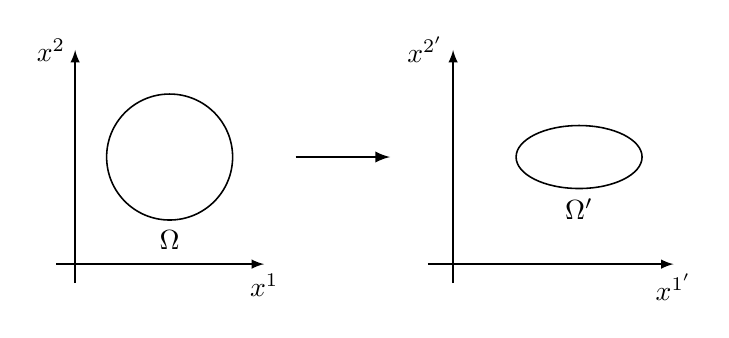
\begin{tikzpicture}[thick, scale=0.8]
    \draw[line width = 0.2mm] (0,0) circle (1cm);
    \draw[line width = 0.2mm] (6.5,0) ellipse (1cm and 0.5cm);
%    \draw[line width = 0.2mm] (11,0) ellipse (1cm and 0.5cm);
    \node[below, black] at (0,-1){$\Omega$};
    \node[below, black] at (6.5,-0.5){$\Omega '$};
%    \node[below, black] at (11,-0.5){$\Omega '$};
    \draw[line width = 0.2mm, black, ->, >=latex] (-1.8,-1.7)--(1.5,-1.7) node[below]{$x^{1}$};
    \draw[line width = 0.2mm, black, ->, >=latex] (-1.5,-2)--(-1.5,1.7) node[left]{$x^{2}$};
    \draw[line width = 0.2mm, black, ->, >=latex] (4.1,-1.7)--(8,-1.7) node[below]{$x^{1'}$};
    \draw[line width = 0.2mm, black, ->, >=latex] (4.5,-2)--(4.5,1.7) node[left]{$x^{2'}$};
%    \draw[line width = 0.2mm, black, ->, >=latex] (9,-1.7)--(12.9,-1.7) node[below]{$x^{1}$};
%    \draw[line width = 0.2mm, black, ->, >=latex] (9.4,-2)--(9.4,1.7) node[left]{$x^{2}$};
    \draw[line width = 0.3mm, black, ->, >=latex] (2,0)--(3.5,0);
%    \node[black] at (8.5,0){$=$};
    \end{tikzpicture}
    \caption{Ilustración esquemática de la transformación de la integral de acción invariante.}
    \label{Transformaciones}
\end{figure}
    
%----------------------------------------------------------------------------------------

\noindent
La variación de la densidad lagrangiana (\ref{2.39_a}) determina que la variación de la acción se escriba como
\begin{equation*}
\begin{split}
\delta S\left[ \phi \right] &=\int_{\Omega ^{\prime }}d^{4}x^{\prime }\left[ \mathcal{L}\left( \phi _{r}\left( x\right) ,\partial _{\mu }\phi _{r}\left(x\right) \right) +\delta \mathcal{L}\left( \phi _{r}\left( x\right),\partial _{\mu }\phi _{r}\left( x\right) \right) \right] -\int_{\Omega }d^{4}x\mathcal{L}\left( \phi _{r}\left( x\right) ,\partial _{\mu }\phi_{r}\left( x\right) \right) \\
&=\int_{\Omega ^{\prime }}d^{4}x^{\prime }\mathcal{L}\left( x\right)+\int_{\Omega ^{\prime }}d^{4}x^{\prime }\delta \mathcal{L}\left( x\right)-\int_{\Omega }d^{4}x\mathcal{L}\left( x\right) ~,
\end{split}
\end{equation*}
\noindent
donde se ha definido $\mathcal{L}\left( \phi_{r}\left( x\right) ,\partial _{\mu }\phi_{r}\left( x\right)\right)\equiv \mathcal{L}\left(x\right)$.\\

\noindent
Ahora, la transformación de coordenadas (\ref{2.36}) determina que el elemento de volumen de integración cambie en la siguiente forma,
\begin{equation}
d^{4}x^{\prime }=\left\vert \frac{\partial x^{\prime \mu }}{\partial x^{\nu }}\right\vert d^{4}x~,
\end{equation}
\noindent
siendo $\left\vert \frac{\partial x^{\prime \mu }}{\partial x^{\nu }}\right\vert$ el determinante Jacobiano de la transformación de coordenadas. Para hallar este determinante se parte de la expresión,
\begin{eqnarray}
\frac{\partial x^{\prime \mu }}{\partial x^{\nu }} &=&\frac{\partial }{%
\partial x^{\nu }}\left[ x^{\mu }+\delta x^{\mu }\right] =\frac{\partial
x^{\mu }}{\partial x^{\nu }}+\frac{\partial }{\partial x^{\nu }}\delta
x^{\mu }  \notag \\
&=&\delta _{\nu }^{\mu }+\partial _{\nu }\delta x^{\mu }~,
\end{eqnarray}
\noindent
de manera que al considerar aproximaciones a primer orden,
 
\begin{eqnarray}
\left\vert \frac{\partial x^{\prime \mu }}{\partial x^{\nu }}\right\vert 
&=&\left\vert \delta _{\nu }^{\mu }+\partial _{\nu }\delta x^{\mu
}\right\vert   \notag \\
&=&\left\vert 
\begin{array}{cccc}
\delta _{0}^{0}+\partial _{0}\delta x^{0} & \delta _{1}^{0}+\partial
_{1}\delta x^{0} & \cdots  & \cdots  \\ 
\delta _{0}^{1}+\partial _{0}\delta x^{1} & \delta _{1}^{1}+\partial
_{1}\delta x^{1} & \cdots  & \cdots  \\ 
\vdots  & \vdots  & \ddots  & \vdots  \\ 
\cdots  & \cdots  & \cdots  & \delta _{3}^{3}+\partial _{3}\delta x^{3}%
\end{array}%
\right\vert   \notag \\
&=&\left\vert 
\begin{array}{cccc}
1+\partial _{0}\delta x^{0} & \partial _{1}\delta x^{0} & \cdots  & \cdots 
\\ 
\partial _{0}\delta x^{1} & 1+\partial _{1}\delta x^{1} & \cdots  & \cdots 
\\ 
\vdots  & \vdots  & \ddots  & \vdots  \\ 
\cdots  & \cdots  & \cdots  & 1+\partial _{3}\delta x^{3}
\end{array}%
\right\vert   \notag \\
&\approx &\left( 1+\partial _{0}\delta x^{0}\right) \left( 1+\partial_{1}\delta x^{2}\right) \left( 1+\partial _{2}\delta x^{2}\right) \left(1+\partial _{3}\delta x^{3}\right)   \notag \\
&\approx &1+\partial _{0}\delta x^{0}+\partial _{1}\delta x^{2}+\partial_{2}\delta x^{2}+\partial _{3}\delta x^{3}  \notag \\
&=&1+\partial _{\mu }\delta x^{\mu }~,
\end{eqnarray}

\noindent
de tal manera que
\begin{equation}
\begin{split}
        d^{4}x^{\prime}&=\left(1+\partial _{\mu }\delta x^{\mu } \right)d^{4}x \\
        &=d^{4}x+d^{4}x\partial _{\mu }\delta x^{\mu }~.
\end{split}
\end{equation}

\noindent
Con base en este resultado la variación de la acción se escribe
\begin{eqnarray}
\delta S[\phi ] &=&\int_{\Omega }\left( d^{4}x+d^{4}x\partial _{\mu }\delta x^{\mu }\right) \mathcal{L}\left( x\right) +\int_{\Omega }\left(d^{4}x+d^{4}x\partial _{\mu }\delta x^{\mu }\right) \delta \mathcal{L}\left(x\right) -\int_{\Omega }d^{4}x\mathcal{L}\left( x\right)   \notag \\
&\approx &\int_{\Omega }d^{4}x\partial _{\mu }\delta x^{\mu }\mathcal{L} \left( x\right) +\int_{\Omega }d^{4}x\delta \mathcal{L}\left( x\right) ~.
\end{eqnarray}
Expresando ahora la variación de la acción en términos de la variación total de la densidad Lagrangiana, la relación (\ref{2.38_aa}) implica 
\begin{equation}
\delta \mathcal{L}\left( x\right) =\tilde{\delta}\mathcal{L}\left( x\right)
+\delta x^{\mu }\partial _{\mu }\mathcal{L}\left( x\right) ~,
\end{equation}
lo que conlleva a deducir:

\begin{eqnarray}
\delta S\left[ \phi \right]  &=&\int_{\Omega }d^{4}x\partial _{\mu }\delta
x^{\mu }\mathcal{L}\left( x\right) +\int_{\Omega }d^{4}x\tilde{\delta}\mathcal{%
L}\left( x\right) +\int_{\Omega }d^{4}x\delta x^{\mu }\partial _{\mu }%
\mathcal{L}\left( x\right)   \notag \\
&=&\int_{\Omega }d^{4}x\partial _{\mu }\left[ \delta x^{\mu }\mathcal{L}%
\left( x\right) \right] +\int_{\Omega }d^{4}x\tilde{\delta}\mathcal{L}\left(
x\right) 
\end{eqnarray}
pero, al expresar la variaci\'{o}n total de la densidad Lagrangiana en t\'{e}rminos de la variaci\'{o}n de los campos y sus derivadas resulta,
\begin{eqnarray*}
\tilde{\delta}\mathcal{L}\left( x\right)  &=&\frac{\partial \mathcal{L}\left(
x\right) }{\partial \phi _{r}}\tilde{\delta}\phi _{r}+\frac{\partial \mathcal{L%
}\left( x\right) }{\partial \left( \partial _{\nu }\phi _{r}\right) }\tilde{%
\delta}\left( \partial _{\nu }\phi _{r}\right) ~,~\ \ \ \ \ \ \ \left[
\partial _{\mu },\tilde{\delta}\right] =0 \\
&=&\frac{\partial \mathcal{L}\left( x\right) }{\partial \phi _{r}}\tilde{\delta%
}\phi _{r}+\frac{\partial \mathcal{L}\left( x\right) }{\partial \left(
\partial _{\nu }\phi _{r}\right) }\partial _{\nu }\tilde{\delta}\phi _{r} \\
&=&\left[ \frac{\partial \mathcal{L}\left( x\right) }{\partial \phi _{r}}%
-\partial _{\nu }\frac{\partial \mathcal{L}\left( x\right) }{\partial \left(
\partial _{\nu }\phi _{r}\right) }\right] \tilde{\delta}\phi _{r}+\frac{%
\partial \mathcal{L}\left( x\right) }{\partial \left( \partial _{\nu }\phi
_{r}\right) }\partial _{\nu }\tilde{\delta}\phi _{r}+\partial _{\nu }\frac{%
\partial \mathcal{L}\left( x\right) }{\partial \left( \partial _{\nu }\phi
_{r}\right) }\tilde{\delta}\phi _{r} \\
&=&\left[ \frac{\partial \mathcal{L}\left( x\right) }{\partial \phi _{r}}%
-\partial _{\nu }\frac{\partial \mathcal{L}\left( x\right) }{\partial \left(
\partial _{\nu }\phi _{r}\right) }\right] \tilde{\delta}\phi _{r}+\partial
_{\nu }\left[ \frac{\partial \mathcal{L}\left( x\right) }{\partial \left(
\partial _{\nu }\phi _{r}\right) }\tilde{\delta}\phi _{r}\right] ~,
\end{eqnarray*}
\noindent
resultado que permite expresar la variaci\'{o}n total de la acci\'{o}n como
\begin{eqnarray*}
\delta S\left[ \phi \right]  &=&\int_{\Omega }d^{4}x\partial _{\mu }\left[\delta x^{\mu }\mathcal{L}\left( x\right) \right] +\int_{\Omega}d^{4}x\left\{ \left[ \frac{\partial \mathcal{L}\left( x\right) }{\partial \phi _{r}}-\partial _{\nu }\frac{\partial \mathcal{L}\left( x\right) }{\partial \left( \partial _{\nu }\phi _{r}\right) }\right] \tilde{\delta}\phi
_{r}+\partial _{\nu }\left[ \frac{\partial \mathcal{L}\left( x\right) }{\partial \left( \partial _{\nu }\phi _{r}\right) }\tilde{\delta}\phi _{r}\right] \right\}  \\
&=&\int_{\Omega }d^{4}x\partial _{\mu }\left[ \delta x^{\mu }\mathcal{L}\left( x\right) +\frac{\partial \mathcal{L}\left( x\right) }{\partial \left(\partial _{\mu }\phi _{r}\right) }\tilde{\delta}\phi _{r}\right] +\int_{\Omega}d^{4}x \left[ \frac{\partial \mathcal{L}\left( x\right) }{\partial \phi _{r}}-\partial _{\nu }\frac{\partial \mathcal{L}\left( x\right) }{\partial \left( \partial _{\nu }\phi _{r}\right) }\right] \tilde{\delta}\phi_{r} ~,
\end{eqnarray*}
al escribir la variación total del campo $\phi_{r}$ con base en (\ref{2.38_aa}), la expresión anterior se transforma en,

\begin{eqnarray}
\delta S\left[ \phi \right]  &=&\int_{\Omega }d^{4}x~\partial _{\mu }\left[ \frac{\partial \mathcal{L}\left( x\right) }{\partial \left( \partial _{\mu}\phi _{r}\right) }\left( \delta \phi _{r}-\delta x^{\nu }\partial _{\nu
}\phi _{r}\left( x\right) \right) +\delta x^{\mu }\mathcal{L}\left( x\right) \right]   \notag \\
&&+\int_{\Omega }d^{4}x\left[ \frac{\partial \mathcal{L}\left( x\right) }{\partial \phi _{r}}-\partial _{\nu }\frac{\partial \mathcal{L}\left(x\right) }{\partial \left( \partial _{\nu }\phi _{r}\right) }\right] \tilde{\delta}\phi _{r}  \notag \\
&=&\int_{\Omega }d^{4}x~\left\{ \partial _{\mu }\left[ \frac{\partial \mathcal{L}\left( x\right) }{\partial \left( \partial _{\mu }\phi_{r}\right) }\delta \phi _{r}-\delta x^{\nu }\left( \frac{\partial \mathcal{L%
}\left( x\right) }{\partial \left( \partial _{\mu }\phi _{r}\right) }\partial _{\nu }\phi _{r}\left( x\right) -g_{~\nu }^{\mu }\mathcal{L}\left(x\right) \right) \right] \right.   \notag \\
&&+\left. \left[ \frac{\partial \mathcal{L}\left( x\right) }{\partial \phi_{r}}-\partial _{\nu }\frac{\partial \mathcal{L}\left( x\right) }{\partial\left( \partial _{\nu }\phi _{r}\right) }\right] \tilde{\delta}\phi_{r}\right\} ~.
\end{eqnarray}

\noindent
Aquí se debe recordar lo planteado en la definición (\ref{definoether}) de simetría, en la cual ante las transformaciones (\ref{2.36}) y (\ref{2.37}) se debe garantizar la coovarianza de la densidad Lagrangiana y que la acción permanezca invariante, de manera que

\begin{equation}
    \delta S \left[\phi \right] = 0~,
\end{equation}
lo que conlleva a
\begin{equation}
    \begin{split}
    \delta S \left[\phi \right] &=\int_{\Omega }d^{4}x~\left\{ \partial _{\mu }\left[ \frac{\partial \mathcal{L}\left( x\right) }{\partial \left( \partial _{\mu }\phi_{r}\right) }\delta \phi _{r}-\delta x^{\nu }\left( \frac{\partial \mathcal{L}\left( x\right) }{\partial \left( \partial _{\mu }\phi _{r}\right) } \partial _{\nu }\phi _{r}\left( x\right) -g_{~\nu }^{\mu }\mathcal{L}\left(x\right) \right) \right] \right.   \\
    &+\left. \left[ \frac{\partial \mathcal{L}\left( x\right) }{\partial \phi_{r}}-\partial _{\nu }\frac{\partial \mathcal{L}\left( x\right) }{\partial \left( \partial _{\nu }\phi _{r}\right) }\right] \tilde{\delta}\phi_{r}\right\}=0 ~. \label{vaccion}
    \end{split}
\end{equation}

\noindent
Se debe tener presente que el volumen de integración $\Omega$ es completamente arbitrario, por ende el integrando de (\ref{vaccion}) deberá desaparecer si la acción es invariante por las transformaciones consideradas, de modo que se debe cumplir:
\begin{equation}
    \partial_{\mu}f^{\mu}(x)+\left( \frac{\partial \mathcal{L}\left( x\right) }{\partial \phi_{r}}-\partial _{\nu }\frac{\partial \mathcal{L}\left( x\right) }{\partial \left( \partial _{\nu }\phi _{r}\right) }\right)\bar{\delta}\phi_{r}=0~,
    \label{intcero}
\end{equation}
\noindent
donde se define el campo vectorial dependiente de las coordenadas,
\begin{equation}
\boxed{
    f^{\mu}(x) \equiv \frac{\partial \mathcal{L}\left( x\right) }{\partial \left( \partial _{\mu }\phi_{r}\right) }\delta \phi _{r}(x)-\delta x^{\nu }\left( \frac{\partial \mathcal{L}\left( x\right) }{\partial \left( \partial _{\mu }\phi _{r}\right) } \partial _{\nu }\phi _{r}\left( x\right) -g_{~\nu }^{\mu }\mathcal{L}\left(x\right) \right)~,
    \label{fmu}
    }
\end{equation}

\noindent
Si los campos que describen el sistema $\phi_{r}(x)$ satisfacen las ecuaciones de movimiento Euler-Lagrange, el segundo término entre paréntesis de la relación (\ref{intcero}) desaparece, de modo que se obtiene,
\begin{equation}
\boxed{
    \partial_{\mu}f^{\mu}(x)=0~,
    }
\end{equation}
\noindent
Esta expresión representa la \textbf{ecuación de continuidad} para el campo vectorial $f^{\mu}(x)$ que se lo identificará como una \emph{``densidad de corriente''} o \emph{``corriente de Noether''}. Esta ecuación garantizará la existencia de una ley de conservación expresada en forma de ecuación diferencial. Con el fin de observar esto, se integra la ecuación de continuidad sobre el espacio tridimensional, de manera que 

\begin{eqnarray*}
0 &=&\int_{V}d^{3}x~\partial _{\mu }f^{\mu }\left( x\right)
=\int_{V}d^{3}x~\partial _{0}f^{0}\left( x\right) +\int_{V}d^{3}x~\partial_{i}f^{i}\left( x\right)  \\
&=&\int_{V}d^{3}x~\frac{\partial f^{0}\left( x\right) }{\partial x^{0}}+\int_{V}d^{3}x~\partial _{i}f^{i}\left( x\right)  \\
&=&\frac{d}{dx^{0}}\int_{V}d^{3}x~f^{0}\left( x\right) +\int_{V}d^{3}x\div{\vb{f\left( x\right)}}  \\
&=&\frac{d}{dx^{0}}\int_{V}d^{3}x~f^{0}\left( x\right) +\oint_{\mathcal{S}}d\vb{a}\vdot\vb{f}\left(x\right) ~,
\end{eqnarray*}

\noindent
donde se ha utilizado el teorema de la divergencia. Teniendo en cuenta que los campos $\phi_{r}(x)$ y sus derivadas desaparecen sobre la superficie $\mathcal{S}$ que limita al volumen $V$ (que tiende a infinito), la segunda integral de la relación anterior desaparece lo que genera el resultado,
\begin{equation*}
    \frac{d}{dx^{0}}\int_{V}d^{3}x~f^{0}\left( x\right)=\frac{d}{dt}\int_{V}d^{3}x~f^{0}\left( x\right)=0~,
\end{equation*}

\noindent
este resultado permite establecer una carga que se conserva en el tiempo, definida de la forma 
\begin{equation}
\begin{split}
    Q &\equiv \int_{V}d^{3}x~f^{0}\left( x\right) \\ 
    &=\int_{V}d^{3}x~\left\{ \frac{\partial \mathcal{L}\left( x\right) }{\partial \left( \partial _{0 }\phi_{r}\right) }\delta \phi _{r}(x)-\delta x^{\nu }\left( \frac{\partial \mathcal{L}\left( x\right) }{\partial \left( \partial _{0}\phi _{r}\right) } \partial _{\nu }\phi _{r}\left( x\right) -g_{~\nu }^{0 }\mathcal{L}\left(x\right) \right)\right\}~.
    \label{carganoether}
\end{split}
\end{equation}
\noindent
En la literatura (\ref{carganoether}) se denomina carga de Noether y es la expresión que se empleará para determinar la carga conservada bajo diferentes simetrías. Cada uno de los resultados obtenidos se enuncian en el siguiente teorema.

\begin{theorem}[Primer Teorema de Noether]
Cada transformación de simetría continua conduce a una ley de conservación donde la cantidad conservada $Q$ se puede obtener de la densidad Lagrangiana asociada al sistema mediante las expresiones (\ref{fmu}) y (\ref{carganoether}).
\end{theorem}

\vspace{0.4cm}
\subsection{Aplicaciones del Teorema de Noether}
\vspace{0.2cm}

Supongamos que tenemos una transformación infinitesimal, que se escribe en términos de ciertos parámetros $\epsilon^{a}$, que cambia las coordenadas y los campos de la siguiente manera

\begin{eqnarray}
x^{\mu } &\rightarrow &x^{\prime \mu }=x^{\mu }+\delta x^{\mu }\equiv x^{\mu}+\epsilon ^{a}A_{a}^{\mu }\left( x\right) \label{xmue} \\
\phi _{r}\left( x\right)  &\rightarrow &\phi _{r}^{\prime }\left( x^{\prime}\right) =\phi _{r}\left( x\right) +\delta \phi _{r}\left( x\right) \equiv \phi_{r}\left( x\right) +\epsilon ^{a}F_{r,a}\left( x \right) \label{fmue} ,
\end{eqnarray}
\noindent
El índice $a$ etiqueta la cantidad de parámetros infinitesimales, mientras que el índice $r$ el número de campos. Decimos que esta transformación es una simetría si deja invariante la acción.  En dicho caso, el teorema de Noether asegura que
%si hay más de uno o de componentes del campo si el mismo es por ejemplo un espinor de Dirac. 
\begin{equation}
    \partial_{\mu} f^{\mu}_{a}=0~,
\end{equation}
sobre las soluciones de las ecuaciones de movimiento, siendo
\begin{equation}
f^{\mu }(x)=\epsilon^{a}\frac{\partial \mathcal{L}\left( x\right) }{\partial \left(
\partial _{\mu }\phi _{r}\right) }\left[ F_{r,a}\left( x\right) -A_{a}^{\nu
}\left( x\right) \partial _{\nu }\phi _{r}\left( x\right) \right]
+\epsilon^{a} A_{a}^{\mu }\left( x\right) \mathcal{L}\left( x\right) ~.
\end{equation}
Además, la cantidad
\begin{equation}
    Q=\int \dd[3]{x} x f^{0}(x)~,
    \label{eq_2.100}
\end{equation}

\noindent
es una constante de movimiento,  es decir, no cambia en el tiempo (sobre las soluciones de las ecuaciones de movimiento).\\

\noindent
Para entender el teorema y cómo usarlo, se empieza con un ejemplo. Comencemos viendo el caso en el cual se tiene invariancia ante traslaciones.


\subsection{Invarianza ante traslaciones Espacio-Temporales}
La invariancia bajo traslaciones es caracterizada por las siguientes transformaciones en las coordenadas y campos:

%\begin{equation}
%\begin{split}
%    x^{\prime \mu}&=x^{\mu}+\epsilon^{\mu}\\
%    &=x^{\mu}+\epsilon^{\nu}g^{\mu}_{~\nu}~,~~~~~\therefore~~~~\delta x^{\mu}=\epsilon^{\mu}~,
%    \label{xpmut}
%\end{split}
%\end{equation}

\begin{equation}
\begin{split}
x^{\mu } \longmapsto x^{\prime \mu } & = x^{\mu }+\epsilon ^{\mu }~\ \implies \epsilon ^{a}=\epsilon ^{\nu }~;~A_{a}^{\mu }=\delta _{\nu }^{\mu } \\
\phi _{r}\left( x\right)  \longmapsto ~\phi _{r}^{\prime }\left( x^{\prime}\right) & = \phi_{r}\left( x^{\prime }-\epsilon \right) = \phi _{r}\left(x\right) ~\ \implies F_{r,a}=F_{r,\mu }=0.
\label{xpmut}
\end{split}
\end{equation}
\noindent

siendo $\epsilon_{\mu}$ un cuadrivector constante\footnote{Note que según la ecuación (\ref{xmue}), en este caso $A^{\mu}_{\nu}=g^{\mu}_{~\nu}$ y se identifica el índice $a \rightarrow \mu$, porque hay cuatro traslaciones infinitesimales, una por cada dirección del espacio-tiempo.}.

%el cual induce la siguiente transformación en los campos: 

%\begin{equation}
%\phi _{r}\left( x\right) \rightarrow \phi ^{\prime }_{r}\left( x^{\prime}\right) =\phi_{r}\left( x^{\prime %}-\epsilon \right) =\phi_{r}\left( x\right) ~,
%\label{ftr}
%\end{equation}

Observe que la invariancia por traslaciones espacio temporales son consecuencia de la homogeneidad del espacio-tiempo donde la forma del campo es supuesta para no cambiar por traslaciones, por ende las variaciones locales de los campos son nulas\footnote{El hecho que la variación en los campos sea nula implica que la cantidad dada en (\ref{fmue}) sea nula, es decir $F_{r,\mu}=0$.}

%\begin{equation}
%    \delta \phi_{r}(x)=0~.
%    \label{vfitr}
%\end{equation}

\noindent
Hasta aquí, lo único que hicimos fue ver qué sucede con las coordenadas y los campos ante una traslación. Para poder aplicar el teorema de Noether, necesitamos ver si esta es una transformación de simetría, es decir, si deja invariante la acción. En este caso, mostrar esto es sencillo, ya que el mismo Lagrangiano queda invariante, puesto que 

\begin{equation}
    \mathcal{L}^{\prime}\left(x^{\prime}\right) \equiv \mathcal{L}\left[\phi^{\prime}\left(x^{\prime}\right), \frac{\partial \phi^{\prime}}{\partial x^{\prime}}, x^{\prime}\right]=\mathcal{L}\left[\phi(x), \frac{\partial \phi}{\partial x^{\prime}}, x^{\prime}\right]~,
\end{equation}
\noindent
pero como $\epsilon^{\mu}$ es un cuadrivector constante, derivar respecto a $x^{\prime}$ es lo mismo que derivar respecto a $x$, por lo que
\begin{equation}
    \mathcal{L}^{\prime}\left(x^{\prime}\right)=\mathcal{L}\left[\phi(x), \frac{\partial \phi}{\partial x}, x^{\prime}\right]~,
\end{equation}

\noindent
El último término en el corchete, $x^{\prime}$, está puesto porque podría pasar que el Lagrangiano dependiera explícitamente de las coordenadas. En nuestro estudio, se verá que la única dependencia del Lagrangiano en las coordenadas aparece sólo a través de los campos, de modo que podemos obviar eso. De este modo, resulta
\begin{equation}
    \mathcal{L}^{\prime}\left(x^{\prime}\right)=\mathcal{L}\left[\phi(x), \frac{\partial \phi}{\partial x}\right]=\mathcal{L}(x),
\end{equation}
y como $d^{4} x^{\prime}=d^{4} x$ la acción también es invariante. Esto nos dice que las traslaciones son simetrías y entonces hay corrientes conservadas. Recurriendo a la ecuación (\ref{fmu}) y reemplazando las transformaciones (\ref{xpmut}):
%y (\ref{vfitr}):

\begin{equation}
f^{\mu }(x)=-\epsilon ^{\nu }\left( \frac{\partial \mathcal{L}\left(x\right) }{\partial \left( \partial _{\mu }\phi _{r}\right) }\partial _{\nu}\phi _{r}\left( x\right) -g_{~\nu }^{\mu }\mathcal{L}\left( x\right)\right) ~,
\end{equation}

\noindent
de tal manera que la ecuación de continuidad tendrá la siguiente forma
\begin{equation}
    \begin{split}
        \partial_{\mu}f^{\mu}&=\partial_{\mu} \left\{ -\epsilon ^{\nu }\left( \frac{\partial \mathcal{L}\left(x\right) }{\partial \left( \partial _{\mu }\phi _{r}\right) }\partial _{\nu}\phi _{r}\left( x\right) -g_{~\nu }^{\mu }\mathcal{L}\left( x\right)\right) \right\} \\
        &=-\epsilon ^{\nu } \partial_{\mu} \left\{ \left( \frac{\partial \mathcal{L}\left(x\right) }{\partial \left( \partial _{\mu }\phi _{r}\right) }\partial _{\nu}\phi _{r}\left( x\right) -g_{~\nu }^{\mu }\mathcal{L}\left( x\right)\right) \right\}~,
    \end{split}
\end{equation}

\noindent
siendo $\epsilon^{\mu}$ constante, la ecuación de continuidad asociada esta simetría tendrá la forma
\begin{equation}
    \partial_{\mu} \Theta^{\mu}_{~\nu}=0,
    \label{derThe}
\end{equation}
donde se ha definido la siguiente corriente de Noether:
\begin{equation}
\boxed{
    \Theta^{\mu}_{~\nu}\equiv  \frac{\partial \mathcal{L}\left(x\right) }{\partial \left( \partial _{\mu }\phi _{r}\right) }\partial _{\nu}\phi _{r}\left( x\right) -g_{~\nu }^{\mu }\mathcal{L}\left( x\right)~,
    \label{TME}
    }
\end{equation}

\noindent
La relación (\ref{TME}) establece que la corriente de Noether es un tensor de segundo orden y se lo conoce como \emph{tensor canónico de momento-energía}. De la ecuación (\ref{carganoether}) se determina que la correspondiente carga de Noether se deriva cuando $\mu=0$, es decir

\begin{equation}
    Q^{\nu}=\int_{V} d^{3}x \Theta^{0 \nu}(x) \equiv P^{\nu}~,
    \label{eq_2.109}
\end{equation}

\noindent    
de ahí que
\begin{equation}
        Q^{\nu}= \int_{V} d^{3}x \left[ \frac{\partial \mathcal{L}\left(x\right) }{\partial \left( \partial _{0 }\phi _{r}\right) }\partial ^{\nu}\phi _{r}\left( x\right) -g^{0 \nu }\mathcal{L}\left( x\right) \right]~.
\end{equation}

\noindent
Del hecho que $\nu=0,1,2,3$ se determina que existen cuatro cantidades conservadas asociadas a esta simetría y que se identifican como la energía $E$, y el momentum $\mathbf{P}$ del campo, que en notación cuadri-dimensional se expresa en la forma (en unidades naturales)
\begin{equation}
    P^{\nu}=\left(E,\mathbf{P}\right)=\int_{V} d^{3}x \Theta ^{0 \nu} =\text{constante}~.
    \label{PnuT}
\end{equation}

\noindent
De las relaciones (\ref{TME}) y (\ref{PnuT}) se puede determinar que la energía del sistema es
\begin{eqnarray}
E &=&\int_{V}d^{3}x\Theta ^{00}\left( x\right)   \notag \\
&=&\int_{V}\left( \frac{\partial \mathcal{L}\left( x\right) }{\partial \left( \partial _{0}\phi _{r}\right) }\partial ^{0}\phi _{r}\left( x\right)-g^{00}\mathcal{L}\left( x\right) \right)   \notag \\
&=&\int_{V}\left( \frac{\partial \mathcal{L}\left( x\right) }{\partial \dot{\phi}_{r}}\dot{\phi}_{r}\left( x\right)-\mathcal{L}\left( x\right) \right) ~,
\end{eqnarray}
 
 la cual corresponde al Hamiltoniano canónico asociado al sistema y $\Theta^{00}$ es la correspondiente densidad hamiltoniana canónica. (Ver ecuaciones (\ref{HC}) y (\ref{dHC}))\\
  
Observe que el tensor $\Theta^{\mu \nu}$ definido en (\ref{TME}) en algunos casos resulta no ser simétrico. Sin embargo, es posible pasar a un tensor de momento-energía simétrico $T^{\mu \nu}=T^{\nu \mu}$ conocido como tensor de \emph{Belinfante}, agregando un término adecuado que tenga cuadridivergencia nula. El nuevo tensor también satisface la ley de conservación (\ref{derThe}) y genera el mismo $P^{\mu}$.\\
 
 \noindent
Podemos usar esta libertad para construir un tensor de momento-energía que sea simetríco, para ello se define:
 
\begin{equation}
T^{\mu \nu }=\Theta ^{\mu \nu }+\partial _{\sigma }\chi ^{\sigma \mu \nu }~,
\end{equation}%
donde $\chi _{\sigma \mu \nu }$ es un tensor arbitrario antisim\'{e}trico en
sus dos primeros \'{\i}ndices, es decir%
\begin{equation}
\chi ^{\sigma \mu \nu }=-\chi ^{\mu \sigma \nu }~,
\end{equation}

ya que esta condición nos asegura que tenga divergencia nula y que entonces $T^{\mu \nu }$ también será una corriente conservada. En efecto


\begin{eqnarray*}
\partial _{\mu }T^{\mu \nu } &=&\partial _{\mu }\Theta ^{\mu \nu }+\partial
_{\mu }\partial _{\sigma }\chi ^{\sigma \mu \nu } \\
&=&\partial _{\mu }\Theta ^{\mu \nu }+\frac{1}{2}\left( \partial _{\mu
}\partial _{\sigma }\chi ^{\sigma \mu \nu }+\partial _{\mu }\partial
_{\sigma }\chi ^{\sigma \mu \nu }\right)  \\
&=&\partial _{\mu }\Theta ^{\mu \nu }+\frac{1}{2}\left( \partial _{\mu
}\partial _{\sigma }\chi ^{\sigma \mu \nu }+\partial _{\sigma }\partial
_{\mu }\chi ^{\mu \sigma \nu }\right) 
\end{eqnarray*}%
donde $\partial _{\mu }\partial _{\sigma }$ es un tensor sim\'{e}trico en
los \'{\i}ndices $\mu ,\sigma $ dado que,%
\begin{equation*}
S_{\mu \sigma }\equiv \partial _{\mu }\partial _{\sigma }=\frac{\partial }{%
\partial x^{\mu }}\frac{\partial }{\partial x^{\sigma }}=\frac{\partial ^{2}%
}{\partial x^{\mu }\partial x^{\sigma }}=\frac{\partial ^{2}}{\partial
x^{\sigma }\partial x^{\mu }}=\frac{\partial }{\partial x^{\sigma }}\frac{%
\partial }{\partial x^{\mu }}=\partial _{\sigma }\partial _{\mu }=S_{\sigma
\mu }~,
\end{equation*}%
por lo tanto,
\begin{eqnarray*}
\partial _{\mu }T^{\mu \nu } &=&\partial _{\mu }\Theta ^{\mu \nu }+\frac{1}{2%
}\partial _{\mu }\partial _{\sigma }\underset{\chi ^{\sigma \mu \nu }-\chi
^{\sigma \mu \nu }=0}{\underbrace{\left( \chi ^{\sigma \mu \nu }+\chi ^{\mu
\sigma \nu }\right) }} \\
&=&\partial _{\mu }\Theta ^{\mu \nu } =0~,
\end{eqnarray*}

\noindent
verificándose además que $T^{\mu \nu}$ y $\Theta^{\mu \nu}$ tienen las mismas cargas conservadas.\\

En conclusión, la invariancia bajo traslaciones espacio-temporales implica la conservación del cuadrimomento, $P^{\mu}$.


\vspace{1cm}

\subsection{Invarianza de Lorentz o ante rotaciones y boots}

\vspace{0.3cm}

Se ha estudiado como el espacio-tiempo es homogéneo ante traslaciones espacio-temporales, ahora se considerará isótropo ante rotaciones, por lo tanto, la acción que se requiere debe ser invariante bajo transformaciones de Lorentz. Estas trasformaciones incluyen además de las usuales rotaciones en el espacio tridimensional, transformaciones en la velocidad (\emph{Boosts de Lorentz}), que se interpretan como rotaciones en el espacio-tiempo.\\

\noindent
La rotación infinitesimal más general se expresa como:
\begin{equation}
    x^{\prime}_{\mu}=x_{\mu}+\delta\omega_{\mu}^{~\nu} x_{\nu}.
\end{equation}

%\implies \epsilon^{a} = \omega^{\mu \nu}
%de manera que $\delta x_{\mu}=x^{\prime}_{\mu}-x_{\mu}=\delta \omega_{\mu}^{~\nu}x_{\nu}$.\\

La cantidad $\delta \omega^{\mu \nu}$ dependiente de los ángulos de rotación en el espacio tiempo.
Para garantizar la invariancia en la magnitud del vector $x^{\mu}$ ante una rotación en el espacio de Minkowski, el tensor $\omega^{\mu \nu}$ debe ser antisimétrico. Para ver esto partimos de la condición

\begin{equation}
    x^{\prime 2}=x^{2}~\implies ~g_{\mu \nu }x^{\prime \mu }x^{\prime \nu
}=g_{\alpha \beta }x^{\alpha }x^{\beta },
\end{equation}

donde

\begin{equation}
    \begin{split}
    g_{\mu \nu }x^{\prime \mu }x^{\prime \nu } & = g_{\mu \nu }\left( x^{\mu}+\delta \omega ^{\mu \alpha }x_{\alpha }\right) \left( x^{\nu }+\delta \omega ^{\nu \beta }x_{\beta }\right)  \\
    & \approx g_{\mu \nu }x^{\mu }x^{\nu }+2\delta \omega ^{\mu \nu }x_{\mu}x_{\nu }.
    \end{split}
    \label{eq2.117}
\end{equation}

la ecuación (\ref{eq2.117}) se garantiza si $\delta \omega ^{\mu \nu }x_{\mu}x_{\nu}$ se anula. Para satisfacer esta afirmación se debe cumplir que
\begin{equation}
    \delta \omega ^{\mu \nu }x_{\mu }x_{\nu } = \frac{1}{2}\left( \omega ^{\mu \nu}+\omega ^{\nu \mu }\right) x_{\mu }x_{\nu }+\cancelto{0}{ \frac{1}{2}\left( \omega ^{\mu \nu }-\omega ^{\nu \mu }\right) x_{\mu }x_{\nu }}=0,
    \label{eq2.118}
\end{equation}

pero el tensor $x_{\mu}x_{\nu}$ es simetrico en sus índices $\mu \nu$, por lo tanto el segundo término resulta ser el producto de un tensor simétrico con otro antisimétrico hecho que hace cero dicho término. Por tanto la expresión (\ref{eq2.118}) se garantiza si $\delta \omega ^{\mu \nu }$ es un tensor completamente antisimétrico. 

\begin{equation}
    \delta \omega ^{\mu \nu }=-\delta \omega ^{\nu \mu  }.
    \label{eq2.119}
\end{equation}

Para ver la manera en como transforman los campos se propone que los campos transformados muestren una dependencia lineal sobre los ángulos de rotación presentes en el tensor $\delta \omega ^ {\mu \nu}$ y sobre los campos mismos $\phi_{r}(x)$. Esta dependencia se la propone a partir del siguiente ansatz:

\begin{equation}
    \phi _{r}^{\prime }\left( x^{\prime }\right) =\phi _{r}\left( x\right) + \frac{1}{2}\delta \omega _{\mu \nu }\left( I^{\mu \nu }\right) _{rs}\phi _{s}\left( x\right) ~~~ \implies~~~ \delta \phi_{r}(x) = \frac{1}{2}\delta \omega_{\mu \nu }\left( I^{\mu \nu }\right) _{rs}\phi _{s}\left( x\right) .
    \label{eq2.120}
\end{equation}

En esta expresión se debe tener presente que los campos $\phi_{r}(x)$ transforman de acuerdo a una representación \emph{irreducible del grupo de Lorentz}, por tanto $(I^{\mu \nu})_{ij}$ son elementos de matriz correspondientes al generador infinitesimal\footnote{Estos generadores son la representación de los elementos del grupo de Lorentz sobre el espacio vectorial generado por los campos $\phi$. Un análisis exhaustivo se halla en el apéndice \ref{Apendice_A}.}. Las Cantidades $I^{\mu \nu}$ se identifican como \emph{generadores infinitesimales de la transformación de Lorentz}, tensor de segundo orden que se caracteriza por ser antisimétrico, consecuencia de (\ref{eq2.119}). De este modo $I^{\mu \nu}$ tendrá asociados seis componentes independientes:

\begin{equation}
    \begin{split}
        (\mu,\nu) &= (1,2);(1,3);(2,3)~~\longmapsto ~\text{Rotaciones espaciales}\\
        (\mu,\nu) &= (0,1);(0,2);(0,3)~~\longmapsto ~\text{Boost de Lorentz}.\\
    \end{split}
\end{equation}

Al ser $I^{\mu \nu}$ un conjunto de generadores infinitesimales del grupo de Lorentz en el álgebra de Lie, se satisface la relación de anticonmutación:
\begin{equation*}
    \comm{I^{\mu \nu}}{I^{\sigma \tau}}=g^{\nu \sigma}I^{\sigma \tau}+g^{\mu \tau}I^{\nu \sigma} - g^{\nu \tau}I^{\mu \sigma}-g^{\mu \sigma}I^{\nu \tau}.
\end{equation*}
Por tanto, esta álgebra de Lie define la estructura de grupo de Lorentz y es válida en cualquer representación.\\

Ahora, la corriente de Noether (ver (\ref{fmu})) asociada a esta simetría es:

\begin{equation}
    \begin{split}
    f^{\mu}(x) &= \pdv{\mathcal{L}}{(\partial_{\mu}\phi_{r})} \qty[\frac{1}{2} \delta \omega_{\alpha \beta} \qty(I^{\alpha \beta})_{rs}\phi_{s}(x)]-\delta \omega^{\nu \alpha}x_{\alpha} \qty[\pdv{\mathcal{L}}{(\partial_{\mu}\phi_{r})}\partial_{\nu}\phi_{r}(x)-g^{\mu}_{~\nu}\mathcal{L}(x)]\\
    &= \frac{1}{2} \pdv{\mathcal{L}}{(\partial_{\mu}\phi_{r})}\delta \omega_{\alpha \beta} \qty(I^{\alpha \beta})_{rs}\phi_{s}(x)-\Theta^{\mu}_{\nu}\delta x^{\alpha} \omega_{\nu \alpha}
    \end{split}
    \label{eq2.122}
\end{equation}

donde se ha empleado la definición del tensor energía-momento (\ref{TME}). Sin embargo, se puede realizar una antisimetrización en el tensor $\Theta^{\mu \nu}x^{\alpha}$ empleando \ref{eq2.119}, de la siguiente manera:

\begin{equation}
    \begin{split}
        \Theta ^{\mu \nu }x^{\alpha }\delta \omega _{\nu \alpha } &= \cancelto{0}{
        \frac{1}{2} \qty(\Theta ^{\mu \nu }x^{\alpha }+\Theta ^{\mu \alpha }x^{\nu })\delta \omega_{\nu \alpha }}+\frac{1}{2} \qty(\Theta ^{\mu \nu }x^{\alpha }-\Theta ^{\mu \alpha}x^{\nu })\delta \omega _{\nu \alpha } \\
        &= \frac{1}{2}(\Theta ^{\mu \nu }x^{\alpha }-\Theta ^{\mu \alpha }x^{\nu})\delta \omega _{\nu \alpha },
    \end{split}
\end{equation}
resultado que se deriva del hecho que $\qty(\Theta ^{\mu \nu }x^{\alpha }+\Theta ^{\mu \alpha }x^{\nu })$ es un tensor simétrico en los índices $\nu \alpha$. Así en (\ref{eq2.122}):
\begin{equation*}
    \begin{split}
        f^{\mu }(x) &= \frac{1}{2}\frac{\partial \mathcal{L}}{\partial \left( \partial _{\mu }\phi _{r}\right) }\delta \omega _{\alpha \beta } \qty(I^{\alpha \beta })_{rs}\phi _{s}\left( x\right) -\frac{1}{2} \qty(\Theta ^{\mu \nu }x^{\alpha }-\Theta ^{\mu \alpha }x^{\nu })\delta \omega _{\nu \alpha } \\
        &= \frac{1}{2}\delta \omega _{\alpha \beta } \qty[\Theta ^{\mu \beta }x^{\alpha }-\Theta ^{\mu \alpha }x^{\beta}+\frac{\partial \mathcal{L}}{\partial \left( \partial _{\mu }\phi _{r}\right) } \qty(I^{\alpha \beta })_{rs}\phi_{s}\left( x\right) ] \\
        &= \frac{1}{2}\delta \omega _{\alpha \beta }M^{\mu \alpha \beta },
    \end{split}
\end{equation*}
siendo $M^{\mu \alpha \beta}$ un tensor de tercer orden definido como:
\begin{equation}
    M^{\mu \alpha \beta }\equiv \qty[\Theta ^{\mu \beta }x^{\alpha }-\Theta ^{\mu \alpha }x^{\beta}+\frac{\partial \mathcal{L}}{\partial \left( \partial _{\mu }\phi _{r}\right) } \qty(I^{\alpha \beta })_{rs}\phi_{s}\left( x\right)],
    \label{TenM}
\end{equation}
en ese orden de ideas, la corriente de Noether correspondiente a esta transformación de simetría es:
\begin{equation}
    f^{\mu}(x)=\frac{1}{2}\delta \omega_{\alpha}{\beta}M^{\mu \alpha \beta}.
    \label{corrM}
\end{equation}
Con esta corriente de Noether y suponiendo que los elementos del tensor $\delta \omega_{\alpha \beta}$ sean constantes, la ecuación de continuidad asociada es:
\begin{equation*}
    \frac{1}{2}\partial _{\mu }[\delta \omega _{\alpha \beta }M^{\mu \alpha \beta }] = 0~\ \implies ~\ \frac{1}{2}\delta \omega _{\alpha \beta }\partial_{\mu }M^{\mu \alpha \beta }=0
\end{equation*}
\begin{equation}
        \boxed{
    ~\therefore ~\partial _{\mu }M^{\mu \alpha \beta } = 0.}
\end{equation}
Esta es la ecuación de continuidad asociada a una simetría ante rotaciones y boost, $M^{\mu \alpha \beta}$ representa la \emph{densidad tensorial de \textbf{momento angular - spin}}. Así, la ``carga'' conservada (ver (\ref{carganoether})) es

\begin{equation}
\boxed{
    M^{\alpha \beta} \equiv \int_{V} \dd[3]{x} M^{0 \alpha \beta} (x)~,
    }
    \label{eq_2.127}
\end{equation}

cantidad que representa el tensor \emph{momento angular - spin}. Observe que

\begin{equation}
    M^{\alpha \beta }=\int_{V} \dd[3]{x} \qty[\Theta ^{0\beta }x^{\alpha }-\Theta ^{0\alpha}x^{\beta }]+\int_{V} \dd[3]{x} \pdv{\mathcal{L}}{\qty(\partial_{0}\phi_{r})} \qty(I^{\alpha \beta })_{rs}\phi _{s}(x)\equiv L^{\alpha \beta }+S^{\alpha \beta },
\end{equation}
\begin{equation*}
    \therefore ~ L^{\alpha \beta} = \int_{V} \dd[3]{x} \qty[\Theta ^{0\beta }x^{\alpha }-\Theta ^{0\alpha}x^{\beta }] ~~ \text{y} ~~ S^{\alpha \beta} = \int_{V} \dd[3]{x} \pdv{\mathcal{L}}{\qty(\partial_{0}\phi_{r})} \qty(I^{\alpha \beta })_{rs}\phi _{s}(x).
\end{equation*}

Para entender mejor el tensor $L^{\alpha \beta}$, se considera las componentes espaciales del mismo y la representación del tensor energía-momento dada en (\ref{TME}), así:
\begin{equation}
    \begin{split}
        L^{km} &= \int_{V} \dd[3]{x} \qty[\Theta ^{0m}x^{k}-\Theta ^{0k}x^{m}] \\
        &= \int_{V} \dd[3]{x} \qty{ \qty[\frac{\partial \mathcal{L(}x)}{\partial (\partial _{0}\phi _{r})}\partial ^{m}\phi_{r}]x^{k}-\qty[\frac{\partial \mathcal{L(}x)}{\partial (\partial _{0}\phi _{r})} \partial ^{k}\phi _{r}(x)]x^{m}} \\
        &= \int_{V}\frac{\partial \mathcal{L(}x)}{\partial \dot{\phi}_{r}} \qty[x^{k}\partial ^{m}-x^{m}\partial ^{k}]\phi _{r}(x)~,
    \end{split}
    \label{eq2.129}
\end{equation}
Este último término se reduce al producto vectorial entre el vector de posición y la densidad de momento, lo que quiere decir que $L^{km}$ representa el \emph{momento angular orbital} ortogonal al plano generado por $x^{k}$ y $x^{m}$. Por otro lado
\begin{equation}
    S^{k m} = \int_{V} \dd[3]{x} \pdv{\mathcal{L}}{\dot{\phi_{r}}} \qty(I^{k m})_{rs}\phi _{s}(x)~,
    \label{eq2.130}
\end{equation}
esta asociado con el \emph{momento angular de spin del campo}\footnote{Al representar el momento angular de spín, su representación es diferente para un campo escalar, vectorial o espinorial.} y tiene explícitos los generadores $\qty(I^{k m})_{rs}$, por ende depende de la forma en como se transforman los campos $\phi_{s}(x)$. Además el tensor $M^{\alpha \beta}$ posee tres cantidades adicionales que se conservan y resultan de la mezcla de los índices espaciales y temporales. Dichas cantidades están relacionadas con la generalización relativista del centro de masa. 


%-------Analizar ejercicio ----------

 %\begin{exercise}[Análisis del campo de Dirac]
 %Halle la expresión de la carga conservada asociada a la invariancia ante rotaciones en el caso del Lagrangiano 5de Dirac. Distinga la contribución a la carga conservada de la parte orbital e intrínseca (Presencia o ausencia %respectivamente de derivadas espaciales) 
 %\end{exercise}

%En la siguiente sección se tratará en mas detalle las teoría de campo relativistas. sin embargo, el Lagrangiano %de Dirac es de la forma:
%\begin{equation}
%   \mathcal{L}_{Dirac} = i \bar{\psi}\gamma^{\mu}\partial_{\mu}\psi-m\bar{\psi}\psi~.
%\end{equation}

%En el apéndice de teoría de grupo \ref{A1}, una transformación de Lorentz en las coordenadas puede escribirse como:
%\begin{equation}
%    x^{\mu} \rightarrow x^{\prime \mu} = \Lambda^{\mu}_{~\nu}x^{\nu}~,
%\end{equation}
%donde
%\begin{equation}
%    \Lambda^{\mu}_{~\nu} = \qty( e^{\frac{i}{2} \omega_{\alpha \beta} M^{\alpha \beta}})^{\mu}_{~\nu}~.
%\end{equation}

\subsection{Simetrías Internas} \label{simint}

Hasta ahora se han considerado simetrías asociadas a transformaciones con las coordenadas. Sin embargo la densidad Lagrangiana asociada a un sistema físico puede ser invariante bajo una transformación de simetría que se refiere a una transformación en los campos y que no conecta a cambios espacio-temporales.\\

Esto puede ocurrir cuando el campo que describe el sistema tiene una estructura interna el cual está reflejada en sus componentes $j$. Una transformación de simetría interna infinitesimal implica una mezcla en sus componentes de la siguiente forma:

\begin{equation}
    \boxed{
    \phi_{r}^{\prime}(x^{\prime})= \phi_{r}(x)+\ii \epsilon \lambda_{rs}\phi_{s},}
    \label{eq_2.131}
\end{equation}

que establece:

\begin{equation}
    \delta x_{\mu} = 0 \quad \text{y} \quad \delta \phi_{r}(x) = \ii \epsilon \lambda_{rs}\phi_{s}(x).
\end{equation}

La corriente de Noether correspondientes es

\begin{equation}
    f^{\mu}(x) =\pdv{\lagdn}{\qty(\partial_{\mu}\phi_{r})}\delta\phi_{r}(x) = \ii \epsilon \pdv{\lagdn}{\qty(\partial_{\mu}\phi_{r})}\lambda_{rs}\phi_{s}(x).
\end{equation}

De la ecuación de continuidad se determina que 

\begin{equation}
    \epsilon \partial_{\mu}\qty[\ii \pdv{\lagdn}{\qty(\partial_{\mu}\phi_{r})}\lambda_{rs}\phi_{s}(x)]=0.
\end{equation}

Por lo tanto se determina que la corriente de Noether es 

\begin{equation}
    J^{\mu} \equiv \ii \pdv{\lagdn}{\qty(\partial_{\mu}\phi_{r})}\lambda_{rs}\phi_{s}(x) ,
\end{equation}
 lo que conlleva a una carga conservada de Noether

 \begin{equation} 
     Q \equiv \int_{V} \dd[3]{x} J^{0}(x) =  \ii \int_{V} \dd[3]{x} \pdv{\lagdn}{\qty(\partial_{0}\phi_{r})}\lambda_{rs}\phi_{s}(x) .
 \end{equation}

Por ejemplo dado un campo escalar complejo descrito por la densidad Lagrangiana

\begin{equation}
    \lagdn = \partial_{\mu}\phi^{*}\partial^{\mu}\phi - m^{2} \phi^{*} \phi,
    \label{eq_2.137}
\end{equation}

donde $\phi^{*}$ y $\phi$ se consideran campos independientes y $m$ es un parámetro constante. Si se considera la transformación:

\begin{equation}
    \phi^{\prime} = \phi~\ee^{\ii \epsilon} \quad \phi^{* \prime} = \phi^{*}~\ee^{-\ii \epsilon}
    \label{SimInt}
\end{equation}
$\lagdn$ es invariante, pues

\begin{IEEEeqnarray}{rCl}
    \lagdn^{\prime} & = & \partial_{\mu}\phi^{* \prime}\partial^{\mu}\phi^\prime - m^{2} \phi^{*\prime}\phi^\prime \notag \\
    & = & \partial_{\mu} \qty[\phi^{*}~\ee^{-\ii \epsilon}]\partial^{\mu}\qty[\phi~\ee^{\ii \epsilon}] \notag\\
    & = & \ee^{-\ii \epsilon}\ee^{\ii \epsilon} - \ee^{-\ii \epsilon}\ee^{\ii \epsilon} m^2 \phi_{*}\phi \notag \\
    & = & \lagdn. \notag
\end{IEEEeqnarray}

lo que implica la existencia de una cantidad conservada. Observe que al ser $\epsilon$ infinitesimal
\begin{equation}
    \phi_1 \mapsto \phi^{\prime} = \phi + \ii\epsilon \phi \quad\quad \phi_2 \mapsto \phi^{* \prime} = \phi^* - \ii \epsilon \phi^* ,
    \label{eq_2.139}
\end{equation}

interpretando $\phi_1 \mapsto \phi$, $\phi_2 \mapsto \phi^{*}$ y comparando este resultado con (\ref{eq_2.131}), se deduce que

\begin{IEEEeqnarray}{rCl}
    \phi_{1}^{\prime} & = & \phi_{1}+\ii \epsilon \lambda_{11}\phi_{1}+\ii \epsilon \lambda_{12}\phi_{2}=\phi+\ii \epsilon \lambda_{11}\phi+\ii \epsilon \lambda_{12}\phi^{*} \notag \\
    \phi_{2}^{\prime} & = & \phi_{2}+\ii \epsilon \lambda_{21}\phi_{1}+\ii \epsilon \lambda_{22}\phi_{2}=\phi^* +\ii \epsilon \lambda_{21}\phi+\ii \epsilon \lambda_{22}\phi^{*}, \notag 
\end{IEEEeqnarray}

resultado que debe coincidir con (\ref{eq_2.139}), por ende se determinan los valores $\lambda_{rs}$,

\begin{equation}
    \lambda_{11}=1=-\lambda_{22} \quad\quad \lambda_{12}=\lambda_{21}=0.
\end{equation}
Con estos resultados la corriente de Noether asociada a la simetría en consideración es

\begin{IEEEeqnarray}{rCl}
    J^\mu & = &  \ii \pdv{\lagdn}{\qty(\partial_{\mu}\phi_{r})}\lambda_{rs}\phi_{s} = \ii \qty[ \pdv{\lagdn}{\qty(\partial_{\mu}\phi_{1})}\lambda_{11}\phi_{1} + \pdv{\lagdn}{\qty(\partial_{\mu}\phi_{2})}\lambda_{22}\phi_{2} ] \notag \\
    %%
    & = & \ii \qty[ \pdv{\lagdn}{\qty(\partial_{\mu}\phi)} \phi - \pdv{\lagdn}{\qty(\partial_{\mu}\phi^*)} \phi^* ] . \notag 
\end{IEEEeqnarray}

Resta evaluar dichas derivadas, para ello se emplea (\ref{eq_2.137}). Así:

\begin{IEEEeqnarray}{rCl}
    \pdv{\lagdn}{\qty(\partial_{\mu}\phi)} & = & \pdv{\qty(\partial_{\mu}\phi)}\qty\bigg[\partial_{\nu}\phi^{*}\partial^{\nu}\phi] = \partial^{\nu}\phi^{*} \pdv{\qty(\partial_{\nu}\phi)}{\qty(\partial_{\mu}\phi)} = \partial^{\nu}\phi^{*} g^{\mu}_{~\nu} =\partial^{\mu}\phi^{*} \notag \\
    %%
    \pdv{\lagdn}{\qty(\partial_{\mu}\phi^*)} & = & \pdv{\qty(\partial_{\mu}\phi^*)}\qty\bigg[\partial_{\nu}\phi^{*}\partial^{\nu}\phi] = \partial^{\nu}\phi \pdv{\qty(\partial_{\nu}\phi^{*})}{\qty(\partial_{\mu}\phi)} = \partial^{\nu}\phi g^{\mu}_{~\nu} =\partial^{\mu}\phi. \notag 
\end{IEEEeqnarray}

Por lo tanto
\begin{equation}
    J^{\mu} = \ii \qty\big[\phi \partial^{\mu}\phi^{*} - \phi^{*} \partial^{\mu}\phi].
\end{equation}

Se puede demostrar del mismo modo que la carga conservada es
\begin{equation}
    Q = \ii \int_{V} \dd[3]{x} \qty\big[\phi \partial^{0}\phi^{*} - \phi^{*} \partial^{0}\phi].
\end{equation}

\subsection{Simetrías de Poincare}

Se considera que el espacio-tiempo es en simultaneo invariante por traslaciones y rotaciones espacio temporales (Homogéneo e isótropo), que conllevó a la conservación del cuadrimomento y el tensor momento angular-espin. En el apéndice \ref{Apendice_A} se establece que el conjunto de traslaciones espacio temprales, rotaciones espaciales y boots de Lorentz constituyen el grupo de Lorentz inhomogeneo o grupo de Poincare. El grupo dicho define un grupo de Lie constituido por 10 parámetros: 3 ángulos de rotación, 3 boost, 3 cambios espaciales y 1 cambio temporal.\\

Una transformación infinitesimal de Poincaré se caracteriza por los siguientes cambios en las coordenadas y campos

\begin{equation}
    \delta x_\mu=\epsilon_\mu+\delta \omega_{\mu \nu} x^\nu, \quad\quad \delta \phi_r(x)=\frac{1}{2} \delta \omega_{\mu \nu}\left(I^{\mu \nu}\right)_{rs} \phi_s(x),
\end{equation}

donde $\delta \omega_{\mu \nu}$ es un tensor antisimétrico de segundo orden. La correspondiente corriente conservada es dada por

\begin{IEEEeqnarray}{rCl} 
    f^\mu(x) & = & \frac{1}{2} \frac{\partial \lagdn}{\partial\qty(\partial_\mu \phi_r)} \delta \omega_{\mu \nu}\left(I^{\mu \nu}\right)_{rs} \phi_s(x)-\qty( \epsilon^\nu+\delta \omega^{\nu \alpha} x_\alpha ) \qty[ \frac{ \partial \lagdn}{\partial \qty(\partial_\mu \phi_{r})} \partial_\nu \phi_r(x)-g^\mu_{~\nu} \lagdn(x) ] \notag \\
    %%
    & = & -\epsilon^\nu \Theta_{~\nu}^\mu+ \frac{1}{2} \frac{\partial \mathcal{L}}{\partial\left(\partial_\mu \phi_r\right)} \delta \omega_{\mu \nu}\left(I^{\mu \nu}\right)_{r s} \phi_s(x)-\delta \omega^{\nu \alpha} x_\alpha \Theta_{~\nu}^\mu \notag \\
    %%
    &=&-\epsilon^\nu \Theta_\nu^\mu+ \frac{1}{2} \frac{\partial \mathcal{L}}{\partial\left(\partial_\mu \phi_r\right)} \delta \omega_{\mu \nu}\left(I^{\mu \nu}\right)_{r s} \phi_s(x)-\frac{1}{2}\left(\Theta^{\mu \nu} x^\alpha-\Theta^{\mu \alpha} x^\nu\right) \delta \omega_{\nu \alpha},
\end{IEEEeqnarray}

donde se ha antisimetrizado la expresión $\Theta^{\mu \nu}x^\alpha$ en los índices $\nu,~\alpha$. Así la corriente de Noether asociada a esta simetría es

\begin{equation}
    f^\mu(x) = - \epsilon_{\nu}\Theta^{\mu \nu}+\frac{1}{2} \delta \omega_{\alpha \beta} \qty\Big[
    \Theta^{\mu \beta}x^\alpha -\Theta^{\mu \alpha}x^\beta+\pdv{\lagdn}{\qty(\partial_{\mu}\phi_r)}\qty(I^{\alpha \beta})_{rs} \phi_{s}].
    \label{eq_2.145}
\end{equation}

A partir de este resultado, la carga conservada se calcula de (\ref{eq_2.100}) como

\begin{IEEEeqnarray}{rCl}
    \int_{V} \dd[3]{x} f^{0} & = &  - \epsilon_{\nu} \int_{V} \dd[3]{x} \Theta^{0 \nu} +\frac{1}{2} \delta \omega_{\alpha \beta} \int_{V} \dd[3]{x} \qty\Big[
    \Theta^{0 \beta}x^\alpha -\Theta^{0 \alpha}x^\beta+\pdv{\lagdn}{\qty(\partial_{0}\phi_r)}\qty(I^{\alpha \beta})_{rs} \phi_{s}]. $\IEEEeqnarraynumspace$
\end{IEEEeqnarray}
Y de las expresiones (\ref{eq_2.109}) y (\ref{eq_2.127}), se deduce que la carga de Noether correspondiente a una simetría de Poincaré es

\begin{equation}
    G = -\epsilon_{\nu} P^\nu+\frac{1}{2} \delta \omega_{\alpha \beta} M^{\alpha \beta}.
\end{equation}
A $G$ se le conoce como \emph{generador del grupo de Poincare}, en cuanto que a $P^\nu$ y $M^{\alpha \beta}$ representan los generadores del grupo de traslaciones y grupo de Lorentz respectivamente. Los generadores de este grupo constituyen el álgebra de Poincare. En la teoría clásica de campos, esta álgebra se escribe en términos de los paréntesis de Poisson.

\begin{IEEEeqnarray}{rCl}
    \comm{P_\mu}{P_\nu} & = & 0 \notag \\
    \comm{M_{\mu \nu}}{P_\lambda} & = & g_{\nu \lambda} P_\mu - g_{\mu \lambda} P_\nu \notag\\
    \comm{M_{\mu \nu}}{M_{\sigma \tau}} &=& g_{\nu \sigma}M_{\mu \tau}+g_{\mu \tau}M_{\nu \sigma}-g_{\nu \tau}M_{\mu \sigma}-g_{\mu \sigma}M_{\nu \tau}. \notag
\end{IEEEeqnarray}

\section{Adicional: Segundo Teorema de Noether}
\vspace{0.2cm}

El teorema de Noether que vimos, o Primer Teorema de Noether, dice que por cada transformación que es una simetría (continua) de nuestro sistema podemos encontrar una corriente que se conserva sobre las soluciones de las ecuaciones de movimiento. Hay un segundo teorema de Noether, que da identidades que valen en general, incluso fuera del espectro de soluciones de las ecuaciones de movimiento.\\

Sin entrar en muchos detalles, el Segundo Teorema de Noether dice que si la acción es invariante ante un grupo de transformaciones locales (es decir, que son parametrizadas por un conjunto de funciones $\lambda(x)$, que dependen del punto del espacio-tiempo), existe entonces un conjunto de identidades entre cantidades construidas a partir de la acción, que se conocen como Identidades de Bianchi. Dichas identidades valen en general, aún si los campos que aparecen en ellas no son soluciones de las ecuaciones de movimiento.\\
Cuando el grupo es, por ejemplo, el de transformaciones de gauge del electromagnetismo,


\begin{equation}
    A^\mu \rightarrow A^\mu+\partial^\mu \lambda(x),
\end{equation}

las identidades de Bianchi son simplemente las ecuaciones de Maxwell.





%---------------Borrar---------------------------------------------------



%-------------------------Borrar-------------------------------

%-----------------------Borrar 2-----------------------------------

%-----------------------Borrar 2-----------------------------------
\begin{comment}
\begin{example}
An\'{a}lisis campo escalar complejo

\emph{Solución}

Cualquier campo complejo se describir\'{a} mediante dos partes
independientes, que pueden expresarse como la parte real e imaginaria del
campo o como el campo complejo en s\'{\i} y su conjugado complejo. Se seguir%
\'{a} la \'{u}ltima alternativa. En consecuencia, la densidad lagrangiana y
las funciones asociadas se dar\'{a}n aqu\'{\i} en t\'{e}rminos de dos
variables de campo independientes, $\phi $ y $\phi ^{\ast }$, cada una de
las cuales son 4 escalares. Para este ejemplo particular, se elige la
densidad lagrangiana

\begin{equation}
\mathcal{L}=c^{2}\left( \partial _{\lambda }\phi \right) \left( \partial
^{\lambda }\phi ^{\ast }\right) -\mu _{0}^{2}c^{2}\phi \phi ^{\ast }~~~~~,
\label{Lagragiano 2.64}
\end{equation}

donde $\mu _{0}~\ $es una constante y $\partial _{\lambda }\phi =\frac{%
\partial \phi }{\partial x^{\lambda }}~\ $y \ $\partial ^{\lambda }\phi
^{\ast }=g^{\lambda \nu }\partial _{\nu }\phi =g^{\lambda \nu }\frac{%
\partial \phi }{\partial x^{\nu }}~~~~~.$

\bigskip Observe que, como se requiere, $\mathcal{L}$ es un campo escalar.
Expresado en t\'{e}rminos de variables de espacio y tiempo, $\mathcal{L}$ se
escribe como

\begin{eqnarray}
\mathcal{L} &=&c^{2}\left( \partial _{\lambda }\phi \right) \left( \partial
^{\lambda }\phi ^{\ast }\right) -\mu _{0}^{2}c^{2}\phi \phi ^{\ast }  \notag
\\
&=&c^{2}\phi _{,0}\phi ^{\ast ,0}+c^{2}\phi _{,i}\phi ^{\ast ,i}-\mu
_{0}^{2}c^{2}\phi \phi ^{\ast }  \notag \\
&=&c^{2}\phi ^{,0}\phi ^{\ast ,0}-c^{2}\phi ^{,i}\phi ^{\ast ,i}-\mu
_{0}^{2}c^{2}\phi \phi ^{\ast }  \notag \\
&=&\frac{c^{2}}{c^{2}}\frac{\partial \phi ^{,}}{\partial t}\frac{\partial
\phi ^{\ast ,}}{\partial t}-c^{2}\frac{\partial \phi ^{,}}{\partial x^{i}}%
\frac{\partial \phi ^{\ast ,}}{\partial x^{i}}-\mu _{0}^{2}c^{2}\phi \phi
^{\ast }  \notag \\
&=&\dot{\phi}\dot{\phi}^{\ast }-c^{2}\nabla \phi \nabla \phi ^{\ast }-\mu
_{0}^{2}c^{2}\phi \phi ^{\ast }~~~~~.  \label{2.65}
\end{eqnarray}%
Para obtener la ecuaci\'{o}n de campo para la cual $\eta _{\rho }=\phi
^{\ast }$, se debe calcular

\begin{eqnarray}
\frac{\partial \mathcal{L}}{\partial \left( \partial _{\nu }\phi ^{\ast
}\right) } &=&\frac{\partial }{\partial \left( \partial _{\nu }\phi ^{\ast
}\right) }\left[ c^{2}\left( \partial _{\lambda }\phi \right) g^{\lambda
\sigma }\left( \partial _{\sigma }\phi ^{\ast }\right) -\mu
_{0}^{2}c^{2}\phi \phi ^{\ast }\right] =c^{2}\frac{\partial }{\partial
\left( \partial _{\nu }\phi ^{\ast }\right) }\left[ \left( \partial
_{\lambda }\phi \right) g^{\lambda \sigma }\left( \partial _{\sigma }\phi
^{\ast }\right) \right]   \notag \\
&=&c^{2}\left( \partial _{\lambda }\phi \right) g^{\lambda \sigma }\frac{%
\partial \left( \partial _{\sigma }\phi ^{\ast }\right) }{\partial \left(
\partial _{\nu }\phi ^{\ast }\right) }=c^{2}\left( \partial _{\lambda }\phi
\right) g^{\lambda \sigma }\delta _{\sigma }^{\nu }=c^{2}\left( \partial
_{\lambda }\phi \right) g^{\lambda \nu }  \notag \\
&=&c^{2}\left( \partial ^{\nu }\phi \right) ~~~~~.  \label{265a}
\end{eqnarray}

y es claro tambi\'{e}n:

\begin{eqnarray}
\frac{\partial \mathcal{L}}{\partial \phi ^{\ast }} &=&\frac{\partial }{%
\partial \phi ^{\ast }}\left[ c^{2}\left( \partial _{\lambda }\phi \right)
g^{\lambda \sigma }\left( \partial _{\sigma }\phi ^{\ast }\right) -\mu
_{0}^{2}c^{2}\phi \phi ^{\ast }\right]   \notag \\
&=&-\mu _{0}^{2}c^{2}\frac{\partial }{\partial \phi ^{\ast }}\left( \phi
\phi ^{\ast }\right) =-\mu _{0}^{2}c^{2}\phi ~~~~~.  \label{2.65b}
\end{eqnarray}

Por tanto, la ecuaci\'{o}n de campo de Euler-Lagrange tiene la forma

\begin{equation}
\frac{\partial \mathcal{L}}{\partial \phi ^{\ast }}-\partial _{\nu }\left( 
\frac{\partial \mathcal{L}}{\partial \left( \partial _{\nu }\phi ^{\ast
}\right) }\right) =0~\ \ \implies ~\ \ -\mu _{0}^{2}c^{2}\phi -c^{2}\left(
\partial _{\nu }\partial ^{\nu }\phi \right) ~=0~~~~~,  \label{2.66}
\end{equation}%
\begin{equation}
c^{2}\left( \partial _{\nu }\partial ^{\nu }\phi \right) +\mu
_{0}^{2}c^{2}\phi =0~~~~~,  \label{2.67}
\end{equation}%
La ecuaci\'{o}n de movimiento de una forma mas conocida se puede expandir de
tal modo que%
\begin{eqnarray*}
c^{2}\left( \frac{1}{c^{2}}\partial _{0}\partial ^{0}\phi -\partial
_{k}\partial ^{k}\phi \right) +\mu _{0}^{2}c^{2}\phi  &=&0 \\
\partial _{0}\partial ^{0}\phi -c^{2}\partial _{k}\partial ^{k}\phi
+c^{2}\mu _{0}^{2}\phi  &=&0
\end{eqnarray*}%
lo que implica,

\begin{equation}
\frac{1}{c^{2}}\frac{\partial ^{2}\phi }{\partial t^{2}}-\nabla ^{2}\phi
+\mu _{0}^{2}\phi =0~~~~~.  \label{2.68}
\end{equation}

En t\'{e}rminos del D'Alembertiano, la expresi\'{o}n (\ref{2.68}) se expresa
como:

\begin{eqnarray}
\frac{1}{c^{2}}\frac{\partial ^{2}\phi }{\partial t^{2}}-\nabla ^{2}\phi
+\mu _{0}^{2}\phi &=&0  \label{2.69} \\
\left[ \frac{1}{c^{2}}\frac{\partial ^{2}}{\partial t^{2}}-\nabla ^{2}\right]
\phi +\mu _{0}^{2}\phi &=&0  \notag \\
\left( \square ^{2}+\mu _{0}^{2}\right) \phi &=&0~~~~~.  \notag
\end{eqnarray}

De manera similar, a partir de la simetr\'{\i}a de $\mathcal{L}$, la ecuaci%
\'{o}n de campo obtenida cuando $\eta _{\rho }=\phi $ ser\'{\i}a:

\begin{eqnarray}
\frac{\partial \mathcal{L}}{\partial \left( \partial _{\nu }\phi \right) }
&=&\frac{\partial }{\partial \left( \partial _{\nu }\phi \right) }\left[
c^{2}\left( \partial _{\lambda }\phi \right) g^{\lambda \sigma }\left(
\partial _{\sigma }\phi ^{\ast }\right) -\mu _{0}^{2}c^{2}\phi \phi ^{\ast }%
\right] =\frac{\partial }{\partial \left( \partial _{\nu }\phi \right) }%
\left[ c^{2}\left( \partial _{\lambda }\phi \right) g^{\lambda \sigma
}\left( \partial _{\sigma }\phi ^{\ast }\right) \right]   \notag \\
&=&c^{2}\frac{\partial \left( \partial _{\lambda }\phi \right) }{\partial
\left( \partial _{\nu }\phi \right) }g^{\lambda \sigma }\left( \partial
_{\sigma }\phi ^{\ast }\right) =c^{2}\delta _{\lambda }^{\nu }g^{\lambda
\sigma }\left( \partial _{\sigma }\phi ^{\ast }\right) =c^{2}g^{\nu \sigma
}\left( \partial _{\sigma }\phi ^{\ast }\right)   \notag \\
&=&c^{2}\left( \partial ^{\nu }\phi ^{\ast }\right) ~~~~~.
\end{eqnarray}

y

\begin{eqnarray}
\frac{\partial \mathcal{L}}{\partial \phi } &=&\frac{\partial }{\partial
\phi }\left[ c^{2}\left( \partial _{\lambda }\phi \right) g^{\lambda \sigma
}\left( \partial _{\sigma }\phi ^{\ast }\right) -\mu _{0}^{2}c^{2}\phi \phi
^{\ast }\right]   \notag \\
&=&-\mu _{0}^{2}c^{2}\frac{\partial }{\partial \phi }\left( \phi \phi ^{\ast
}\right) =-\mu _{0}^{2}c^{2}\phi ^{\ast }~~~~~.
\end{eqnarray}

de manera que la ecuaci\'{o}n de campo es:

\begin{equation}
\frac{\partial \mathcal{L}}{\partial \phi }-\partial _{\nu }\left( \frac{%
\partial \mathcal{L}}{\partial \left( \partial _{\nu }\phi \right) }\right)
=0~\ \implies ~\ -\mu _{0}^{2}c^{2}\phi ^{\ast }-c^{2}\left( \partial _{\nu
}\partial ^{\nu }\phi ^{\ast }\right) =0~~~~~,  \label{2.70}
\end{equation}

lo que quiere decir%
\begin{equation}
\left( \square ^{2}+\mu _{0}^{2}\right) \phi ^{\ast }=0~~~~~.  \label{2.71}
\end{equation}

Esta ecuaci\'{o}n de campo b\'{a}sica satisfecha por $\phi $ y $\phi ^{\ast }
$ se conoce como la ecuaci\'{o}n de Klein-Gordon y, como se indica aqu\'{\i}%
, representa el an\'{a}logo relativista de la ecuaci\'{o}n de Schrodinger
para una part\'{\i}cula cargada de esp\'{\i}n cero y de energ\'{\i}a de masa
en reposo $\mu _{0\text{.}}$

A modo de ejemplo, considerando un campo escalar complejo $\phi $ bajo una
transformaci\'{o}n del tipo:%
\begin{equation}
\phi ^{\prime }=\phi e^{i\epsilon }~\ \ \ \rightarrow \ \ \ \ \ \phi ^{\ast
\prime }=\phi ^{\ast }e^{-i\epsilon }~~~~~,  \label{2.63}
\end{equation}%
la cual corresponde en forma infinitesimal a una transformaci\'{o}n de gauge
de primera especie, dada en la relaci\'{o}n (\ref{2.60}), tal que%
\begin{equation}
c_{\phi }=i~\ \ \ \ \ c_{\phi }^{\ast }=-i~~~~~.
\end{equation}%
Entonces, es obvio que la densidad lagrangiana dada anteriormente es
invariante bajo la transformaci\'{o}n (\ref{2.63}), esto es por que

\begin{eqnarray*}
\mathcal{L}^{\prime } &=&c^{2}\left( \partial _{\lambda }\phi ^{\prime
}\right) \left( \partial ^{\lambda }\phi ^{\prime \ast }\right) -\mu
_{0}^{2}c^{2}\phi ^{\prime }\phi ^{\prime \ast } \\
&=&c^{2}\left( e^{i\epsilon }\partial _{\lambda }\phi \right) \left(
e^{-i\epsilon }\partial ^{\lambda }\phi ^{\ast }\right) -\mu
_{0}^{2}c^{2}\left( e^{i\epsilon }\phi \right) \left( e^{-i\epsilon }\phi
^{\prime \ast }\right)  \\
&=&c^{2}e^{i\epsilon }e^{-i\epsilon }\left( \partial _{\lambda }\phi \right)
\left( \partial ^{\lambda }\phi ^{\ast }\right) -\mu
_{0}^{2}c^{2}e^{i\epsilon }e^{-i\epsilon }\phi \phi ^{\prime \ast } \\
&=&c^{2}\left( \partial _{\lambda }\phi \right) \left( \partial ^{\lambda
}\phi ^{\ast }\right) -\mu _{0}^{2}c^{2}\phi \phi ^{\prime \ast }=\mathcal{L}%
~~~~~.
\end{eqnarray*}%
Por lo tanto, existe una densidad de corriente asociada para el campo de
Klein-Gordon. Para determinar esta corriente, se deben calcular las
cantidades

\begin{equation*}
\delta \eta _{p}=\epsilon c_{\rho }\eta _{\rho }~~~~~.
\end{equation*}

Entonces, para $\phi $

\begin{eqnarray*}
\delta \eta _{\rho } &=&\eta _{\rho }^{\prime }-\eta _{\rho }=e^{i\epsilon
}\phi -\phi \approx \left( 1+i\epsilon \right) \phi -\phi  \\
&=&\phi +i\epsilon \phi -\phi =i\epsilon \phi \equiv c_{\phi }\epsilon \phi
~~~~~
\end{eqnarray*}%
y para $\phi ^{\ast }$

\begin{eqnarray*}
\delta \eta _{\rho } &=&\eta _{\rho }^{\prime }-\eta _{\rho }=e^{-i\epsilon
}\phi ^{\ast }-\phi ^{\ast }\approx \left( 1-i\epsilon \right) \phi ^{\ast
}-\phi ^{\ast } \\
&=&\phi ^{\ast }-i\epsilon \phi ^{\ast }-\phi ^{\ast }=-i\epsilon \phi
^{\ast }\equiv c_{\phi ^{\ast }}\epsilon \phi ^{\ast }~~~~~,
\end{eqnarray*}

de manera que 
\begin{equation*}
c_{\phi }=i~\ \ \ \ \ \ \ c_{\phi ^{\ast }}=-i~~~~~.
\end{equation*}%
lo\ cual corrobora lo planteado anteriormente.

Con lo anterior ya se demuestra entonces que es posible encontrar una
corriente conservada asociada al campo de Klein-Gordon. As\'{\i}, la
corriente conservada viene dada por

\begin{equation*}
\Theta ^{\nu }=c_{\rho }\frac{\partial \mathcal{L}}{\partial \left( \partial
_{\nu }\eta _{\rho }\right) }\eta _{\rho }~~~~~,
\end{equation*}

donde hay una suma implicita sobre $\rho $ , haciendo referencia a todos los
campos: $\eta _{1}=\eta _{\phi }=\phi ~\ $y$~\ \eta _{2}=\eta _{\phi ^{\ast
}}=\phi ^{\ast }$. Se debe cumplir,

\begin{eqnarray*}
\Theta ^{\nu } &=&c_{\phi }\frac{\partial \mathcal{L}}{\partial \left(
\partial _{\nu }\eta _{\phi }\right) }\eta _{\phi }+c_{\phi ^{\ast }}\frac{%
\partial \mathcal{L}}{\partial \left( \partial _{\nu }\eta _{\phi ^{\ast
}}\right) }\eta _{\phi ^{\ast }}=c_{\phi }\frac{\partial \mathcal{L}}{%
\partial \left( \partial _{\nu }\phi \right) }\phi +c_{\phi ^{\ast }}\frac{%
\partial \mathcal{L}}{\partial \left( \partial _{\nu }\phi ^{\ast }\right) }%
\phi ^{\ast } \\
&=&i\frac{\partial \mathcal{L}}{\partial \left( \partial _{\nu }\phi \right) 
}\phi -i\frac{\partial \mathcal{L}}{\partial \left( \partial _{\nu }\phi
^{\ast }\right) }\phi ^{\ast }=ic^{2}\left( \partial ^{\nu }\phi ^{\ast
}\right) \phi -ic^{2}\left( \partial ^{\nu }\phi \right) \phi ^{\ast }~~~~~,
\end{eqnarray*}%
\begin{equation}
\therefore ~\Theta ^{\nu }=ic^{2}\left[ \phi \left( \partial ^{\nu }\phi
^{\ast }\right) -\phi ^{\ast }\left( \partial ^{\nu }\phi \right) \right]
~~~~~,
\end{equation}%
reordenando t\'{e}rminos,

\begin{eqnarray}
g^{\nu \mu }\Theta _{\mu } &=&ic^{2}\left[ \phi g^{\nu \sigma }\left(
\partial _{\sigma }\phi ^{\ast }\right) -\phi ^{\ast }g^{\nu \sigma }\left(
\partial _{\sigma }\phi \right) \frac{{}}{{}}\right]   \notag \\
&=&ic^{2}\left( \phi g^{\nu \sigma }\frac{\partial \phi ^{\ast }}{\partial
x^{\sigma }}-\phi ^{\ast }g^{\nu \sigma }\frac{\partial \phi }{\partial
x^{\sigma }}\right)   \notag \\
&=&ic^{2}g^{\nu \sigma }\left( \phi \frac{\partial \phi ^{\ast }}{\partial
x^{\sigma }}-\phi ^{\ast }\frac{\partial \phi }{\partial x^{\sigma }}\right) 
\notag \\
&=&g^{\nu \mu }\left[ ic^{2}\left( \phi \frac{\partial \phi ^{\ast }}{%
\partial x^{\sigma }}-\phi ^{\ast }\frac{\partial \phi }{\partial x^{\sigma }%
}\right) \right] ~~~~~.
\end{eqnarray}

\begin{remark}
La igualdad se garantiza si la cantidad covariante entre corchetes es igual
a la corriente conservada asociada al campo de Klein-Gordon, es decir:

\begin{equation}
j_{\mu }=iq\left( \phi \frac{\partial \phi ^{\ast }}{\partial x^{\sigma }}%
-\phi ^{\ast }\frac{\partial \phi}{\partial x^{\sigma }}\right)
~~~~~,  \label{2.72}
\end{equation}
\end{remark}

que est\'{a} de acuerdo con la densidad de corriente de la mec\'{a}nica cu%
\'{a}ntica convencional. Tenga en cuenta que la derivaci\'{o}n completa de
la densidad de corriente de carga conservada depende del hecho de que el
campo es complejo. Por lo tanto, como se mencion\'{o} anteriormente, un
campo real no conduce a una carga o densidad de corriente asociada con el
campo. Para describir los campos asociados con part\'{\i}culas cargadas, se
debe usar un par de campos complejos como $\phi $ y $\phi ^{\ast }$ para la
part\'{\i}cula de Klein-Gordon (sin esp\'{\i}n).

Tenga en cuenta que, si bien el teorema de Noether demuestra que una
propiedad de simetr\'{\i}a cont\'{\i}nua de la densidad lagrangiana conduce
a una condici\'{o}n de conservaci\'{o}n, lo contrario no es cierto. Parece
haber condiciones de conservaci\'{o}n que no pueden corresponder a ninguna
propiedad de simetr\'{\i}a. Los ejemplos m\'{a}s destacados en este momento
son los campos que tienen soluciones de solit\'{o}n, por ejemplo, se
describen mediante la ecuaci\'{o}n seno-Gordon o la ecuaci\'{o}n
Korteweg-devries.\\

\fbox{\parbox{14cm}{\textbf{Nota:}
Solit\'{o}n es una onda solitaria que se propaga sin deformarse en un
medio no lineal. Se encuentra en fen\'{o}menos f\'{\i}sicos como soluci\'{o}n 
a ecuaciones diferenciales no lineales.}}
\end{example}

%%***Análisis de Simetria y Teoría de Grupos*** ***Tomar de los apuntes de fisica de particulas***

\section{Formalismo Hamiltoniano en teor\'{\i}a cu\'{a}ntica de Campos}

De aqu\'{\i} en adelante se va a denotar un campo a traves de $\eta _{\rho
}=\Phi ^{A}$.

Los momentos can\'{o}nicos de los campos $\Phi ^{A}$ se definen de forma an%
\'{a}loga a los sistemas con un n\'{u}mero finito de grados de libertad:

\begin{equation}
\Pi _{A}=\frac{\delta L}{\delta \dot{\Phi}^{A}}~~~~~,  \label{2.73}
\end{equation}

donde $\dot{\Phi}^{A}$ representa la derivada de $\Phi ^{A}$ con respecto al
tiempo. Esta es una derivada parcial, ya que $\Phi ^{A}$ depende tambi\'{e}n
de las coordenadas espaciales. Adem\'{a}s, $L$ es funcional, por lo que la
derivada indicada en la Ec. (\ref{2.73}) es realmente la derivada de un
funcional con respecto a una funci\'{o}n, es decir, una derivada funcional.
Evitaremos usar el signo de la derivada parcial para recordar este hecho y
se usar\'{a} el s\'{\i}mbolo $\delta $ en su lugar.

Para realizar la diferenciaci\'{o}n funcional en la Ec. (\ref{2.73}),
necesitamos conocer las derivadas, con respecto a $\dot{\Phi}$'s, de los
campos $\Phi ^{A}$ as\'{\i} como de $\dot{\Phi}^{A}$ y $\nabla \Phi ^{A}$,
ya que estos son los bloques de construcci\'{o}n de $L$. Se toma el ejemplo
de la mec\'{a}nica de part\'{\i}culas, donde las coordenadas generalizadas $%
q_{i}$\ y sus correspondientes velocidades \thinspace $\dot{q}_{i}$ son
variables independientes en el formalismo lagrangiano. En particular, $d\dot{%
q}_{i}/d\dot{q}_{j}=\delta _{ij}$, mientras que $dq_{i}/d\dot{q}_{j}=0$.
Para los campos, reemplazamos el \'{\i}ndice discreto por la coordenada
espacial $\mathbf{x}$ y el \'{\i}ndice $A$ que caracterizan al campo.
Entonces, las derivadas funcionales fundamentales est\'{a}n dadas por:

\begin{equation}
\frac{\delta \dot{\Phi}^{B}\left( t,\mathbf{y}\right) }{\delta \dot{\Phi}%
^{A}(t,\mathbf{x})}=\delta _{B}^{A}\delta ^{3}\left( \mathbf{x}-\mathbf{y}%
\right) ~~~~~,  \label{2.74}
\end{equation}

mientras que las derivadas funcionales de los campos y sus derivadas
espaciales con respecto a $\dot{\Phi}^{A}$ se desvanecen de manera id\'{e}%
ntica. En la Eq. (\ref{2.74}), observe que la derivada funcional de con
respecto a s\'{\i} misma no es adimensional, sino que tiene las dimensiones
de un volumen inverso.

Se introduce ahora el hamiltoniano del sistema, que tambi\'{e}n debe
entenderse que significa realmente la densidad hamiltoniana y se indicar\'{a}
con el s\'{\i}mbolo $\mathcal{H}$. La integral de volumen de $\mathcal{H}$,
que generalmente se llama hamiltoniana en el caso de la din\'{a}mica de part%
\'{\i}culas, se llamar\'{a} hamiltoniana total y se indicar\'{a} con $H$. El
hamiltoniano $\mathcal{H}$ se puede definir en t\'{e}rminos de los momentos
can\'{o}nicos de la siguiente manera:

\begin{equation}
\mathcal{H}\left( \Phi ^{A},\partial _{k}\Phi ^{A},\Pi _{A}\right) =\Pi _{A}%
\dot{\Phi}^{A}-\mathcal{L}\left( \Phi ^{A},\partial _{\mu }\Phi ^{A}\right)
~~~~~.  \label{2.75}
\end{equation}

Observe que el lagrangiano es una funci\'{o}n de los campos y sus derivadas
parciales con respecto a todas las coordenadas del espacio-tiempo. En el
hamiltoniano, las derivadas de campo con respecto al tiempo han sido
reemplazadas por los momentos can\'{o}nicos. Sin embargo, el hamiltoniano
todav\'{\i}a puede ser una funci\'{o}n de las derivadas espaciales. El
hamiltoniano total es funcional en el mismo sentido que el lagrangiano total.

El corchete de Poisson de dos funcioanles cualesquiera $F_{1}$ y $F_{2}$
puede ser definido como:

\begin{equation}
\lbrace  F_{1}\left( \mathbf{x}_{1}\right),F_{2}\left( \mathbf{x}_{2}\right) %
\rbrace =\int d^{3}x\left( \frac{\delta F_{1}\left( \mathbf{x}%
_{1}\right) }{\delta \Phi ^{A}\left( t,\mathbf{x}\right) }\frac{\delta
F_{2}\left( \mathbf{x}_{2}\right) }{\delta \Pi _{A}\left( t,\mathbf{x}%
\right) }-\frac{\delta F_{1}\left( \mathbf{x}_{1}\right) }{\delta \Pi
_{A}\left( t,\mathbf{x}\right) }\frac{\delta F_{2}\left( \mathbf{x}%
_{2}\right) }{\delta \Phi ^{A}\left( t,\mathbf{x}\right) }\right) ~~~~~.
\label{2.76}
\end{equation}

Estas derivadas se pueden reducir a las siguientes fundamentales que son
similares a la relaci\'{o}n (\ref{2.74}):

\begin{equation}
\frac{\delta \Phi ^{B}\left( t,\mathbf{y}\right) }{\delta \Phi ^{A}\left( t,%
\mathbf{x}\right) }=\delta _{A}^{B}\delta ^{3}\left( \mathbf{x-y}\right)
\label{2.77}
\end{equation}

\begin{equation}
\frac{\delta \Pi _{B}\left( t,\mathbf{y}\right) }{\delta \Pi _{A}\left( t,%
\mathbf{x}\right) }=\frac{\delta \left( \frac{\delta L}{\delta \dot{\Phi}^{B}%
}\right) \left( t,\mathbf{y}\right) }{\delta \left( \frac{\delta L}{\delta 
\dot{\Phi}^{A}}\right) \left( t,\mathbf{x}\right) }  \label{2.78}
\end{equation}

\begin{equation}
\frac{\delta \Pi _{B}\left( t,\mathbf{y}\right) }{\delta \Pi _{A}\left( t,%
\mathbf{x}\right) }=\delta _{B}^{A}\delta ^{3}\left( \mathbf{x-y}\right)
~~~~~,  \label{2.79}
\end{equation}

mientras que las derivadas funcionales de los campos con respecto a los
momentos, as\'{\i} como viceversa, se desvanecen. Por ejemplo,

\begin{eqnarray}
\lbrace \Phi ^{A}\left( t,\mathbf{x}\right) ,\Pi _{B}\left( t,\mathbf{y}%
\right) \rbrace &=&\int d^{3}z\left( \frac{\delta \Phi ^{A}\left( t,%
\mathbf{x}\right) }{\delta \Phi ^{C}\left( t,\mathbf{z}\right) }\frac{\delta
\Pi _{B}\left( t,\mathbf{y}\right) }{\delta \Pi _{C}\left( t,\mathbf{z}%
\right) }-\frac{\delta \Phi ^{A}\left( t,\mathbf{x}\right) }{\delta \Pi
_{C}\left( t,\mathbf{z}\right) }\frac{\delta \Pi _{B}\left( t,\mathbf{y}%
\right) }{\delta \Phi ^{C}\left( t,\mathbf{z}\right) }\right)  \label{2.80}
\\
&=&\int d^{3}z\left( \frac{\delta \Phi ^{A}\left( t,\mathbf{x}\right) }{%
\delta \Phi ^{C}\left( t,\mathbf{z}\right) }\frac{\delta \Pi _{B}\left( t,%
\mathbf{y}\right) }{\delta \Pi _{C}\left( t,\mathbf{z}\right) }\right) 
\notag \\
&=&\int d^{3}z\delta _{C}^{A}\delta ^{3}\left( \mathbf{x-z}\right) \delta
_{B}^{C}\delta ^{3}\left( \mathbf{y-z}\right)  \notag \\
&=&\delta _{C}^{A}\delta _{B}^{C}\int d^{3}z\delta ^{3}\left( \mathbf{x-z}%
\right) \delta ^{3}\left( \mathbf{y-z}\right) =\delta _{B}^{A}\delta
^{3}\left( \mathbf{x-y}\right) ~~~~~.  \notag
\end{eqnarray}
\end{comment}

%-----------------------------------------------      Fin Capítulo 2 ------------------------------------------------------------------------------------------- 
%----------------------------------------------------------------------------------------

%----------------------------------------------------------------------------------------
%	CHAPTER 3 Cuantización de Campo Escalar
%----------------------------------------------------------------------------------------
%	CHAPTER 3 Cuantización de Campo Escalar
%----------------------------------------------------------------------------------------

\chapterimage{chapter_head_2.pdf}
\chapter{Cuantización de Campo Escalar}

\newcommand{\ON}{N}
\newcommand{\OH}{H}

\label{capitulo_3}

Habiendo tratado los aspectos necesarios de la teoría clásica de campos, vamos a comenzar a analizar las teorías cuánticas de campos relativistas. Para ello, comenzaremos estudiando la cuantización de teorías libres, es decir, de aquellas para las cuales no aparecen términos de interacción (o sea, términos con tres o más campos) en el Lagrangiano. Una de los motivos por los cuales las teorías libres son relevantes es porque se asume que en los procesos de scattering los estados asintóticos pueden ser descriptos por una teoría libre. Más allá de esto, el estudio de las teorías libres nos permitirá entender algunos aspectos de las teorías cuánticas de campos relativistas.\\

En esta primera parte utilizaremos el método de cuantización canónica. Sobre el final del curso
la idea es presentar otro método de cuantización, el de integrales de camino.\\

Tengan en cuenta que vamos a trabajar en la representación de Heisenberg de la mecánica cuántica: los operadores son los que evolucionan en el tiempo, mientras que los estados están
fijos.

\section{Cuantización canónica del campo escalar real}

Campo escalar es el campo relativista mas simple que se puede introducir. Estos campos se caracterizan por ser invariantes por transformaciones del grupo de Lorentz. De ahora en adelante, utilizaremos las unidades naturales descritas en el primer capitulo.

\subsection{Ecuación de movimiento}

Para derivar la ecuación de movimiento asociada a campo escalar, utilizaremos el análisis que permite derivar la ecuación de Schrödinger en mecánica cuántica
\begin{equation*}
    \ii \hbar \pdv{\psi(t,\vb*{x})}{t} = \qty[-\frac{\hbar^2}{2m}\laplacian + V(\vb*{x}) ] \psi(t,\vb*{x}),
\end{equation*}
que es la versión a nivel de operador de la relación asociada a la energía no relativista
\begin{equation*}
    \hat{E} = \frac{\hat{p}^{2}}{2m} + \hat{V}(\vb*{x}),
\end{equation*}

aplicada a la función de onda $\psi(t,\vb*{x})$ con
\begin{equation}
    \hat{E} \to \ii \hbar \pdv{t}, \quad\quad \hat{p} \to \ii\hbar \grad \, ,
\end{equation}

representaciones de los operadores energía y momento respectivamente. Ahora en el caso relativista se parte de la relación energía-momento relativista que en forma de operador se expresa como

\begin{IEEEeqnarray}{rCl}
    \hat{p}^{\mu}\hat{p}_{\mu} & = & m^{2} \implies \hat{p}^{\mu}\hat{p}_{\mu}-m^{2} =0 \, ,    \label{eq_3.1}
\end{IEEEeqnarray}
donde $m$ denota la masa de la partícula libre en reposo. Este operador deberá actuar sobre el campo $\phi (x)$ considerando a $\hat{p}_\mu \to \ii \partial_\mu$ como la representación del operador momento.\\

Teniendo en cuenta que 

\begin{equation*}
    \hat{p}_\mu \hat{p}^\mu = - \partial_\mu \partial^\mu = -\square \, , 
\end{equation*}

se obtiene la relación

\begin{IEEEeqnarray}{rCl} 
    \left( -\partial ^{\mu }\partial _{\mu }-m^{2}\right) \phi \left( x\right) &=&0  \label{eq_3.3} \\
    \left(\square ^{2}+m^{2}\right) \phi \left( x\right) &=&0  \notag
\end{IEEEeqnarray}

que es conocida como la ecuación de Klein-Gordon (EKG). Esta EKG describe el campo en ausencia de fuente, es decir, sin interacción. El hecho que la EKG sea la versión a nivel de operador del la relación energía momento $ p^{\mu}p_{\mu}= m^{2}$, indica que todo campo relativista deberá satisfacer esta expresión.\\

A simple vista, la EKG parece simple, pero hay un problema, los valores propios de energía son

\begin{equation} 
    p^{\mu}p_{\mu} = m^{2} \quad \implies \quad E^{2}=\vb*{p}^{2}+m^{2}  \quad \implies \quad E = \pm  \sqrt{\vb*{p}^2+m^2}.
    \label{eq_3.4}
\end{equation}

Aquí se tiene que la energía puede ser negativa y su magnitud puede ser arbitrariamente grande ya que $\abs{\vb*{p}}$ no está acotado. Por tanto, el sistema no tendrá estado fundamental y colapsará en valores de energía negativos cada vez mayores y será totalmente inestable. Por tanto, no es posible una interpretación de la función de onda de la EKG. Este problema tendrá una interpretación solo al cuantizar el campo.

\subsection{Cuantización canónica}

La EKG es la correspondiente ecuación de Euler-Lagrange derivada de la densidad Lagrangiana asociada a campo escalar $\phi (x)$, 

\begin{equation}
	\boxed{
    \mathcal{L}=\frac{1}{2}\left( \partial ^{\mu }\phi \right) \left( \partial_{\mu }\phi \right) -\frac{1}{2}m^{2}\phi ^{2} } \, ,
    \label{eq_3.5}
\end{equation}

la cual verifica que

\begin{equation}
    \pdv{\lagdn}{\phi}-\partial_{\mu}\pdv{\lagdn}{\qty(\partial_\mu \phi)}=0 \quad \implies \quad \left(\square^{2}+m^{2}\right) \phi (x) = 0~.
\end{equation}

Al extender la teoría al formalismo Hamiltoniano, se introduce el momento canónico conjugado asociado al campo $\phi$ como siendo

\begin{equation}
    \Pi(x) = \pdv{\lagdn}{\dot{\phi}} = \pdv{\lagdn}{\qty(\partial _{0}\phi)}.
    \label{eq_3.6}
\end{equation}

Empleando la densidad lagrangiana (\ref{eq_3.5}), se tiene que

\begin{IEEEeqnarray}{rCl}
    \Pi (x) &=& \pdv{\qty(\partial_0 \phi)}\qty\bigg[\frac{1}{2} \partial ^{\mu }\phi \partial_{\mu }\phi] \nonumber\\*
    & = & \partial^\mu \phi \pdv{\qty(\partial_\mu \phi)}{\qty(\partial_0 \phi)} = \partial^\mu \phi \delta^0_\mu \nonumber\\*
    & = & \partial^0 \phi = \dot{\phi} (x) \, .
    \label{eq_3.8}
\end{IEEEeqnarray}

El Hamiltoniano canónico asociado a campo escalar real clásico es 

\begin{IEEEeqnarray}{rCl}
    H & = & \int \dd[3]{x} \hamdn = \int \dd[3]{x} \qty\big[\dot{\phi}(x)\Pi (x)-\lagdn],
\end{IEEEeqnarray}
donde
\begin{IEEEeqnarray}{rCl}
    \hamdn &=& \dot{\phi}\Pi-\qty[\frac{1}{2}\partial^\mu\phi \partial_\mu\phi - \frac{1}{2} m^2 \phi^2] \nonumber\\*
    & = & \Pi \Pi-\frac{1}{2}\dot{\phi}\dot{\phi} +\frac{1}{2}\partial^k\phi \partial^k\phi - \frac{1}{2} m^2 \phi^2] \nonumber\\*
    & = & \frac{1}{2}\qty\bigg[\Pi^2+\qty(\grad \phi)^2 + m^2 \phi^2].
    \label{eq_3.10}
\end{IEEEeqnarray}

En mecánica clásica la evolución temporal de una variable dinámica se escribe en términos de su paréntesis de Poisson (PP) entre la variable y el Hamiltoniano canónico. Al generalizar la definición de corchete de Poisson para contemplar el caso en el cual tenemos grados de libertad continuos, introducimos lo que se conoce como derivada funcional, generalización trabajada en el capitulo \ref{capitulo_22}. Así los PP fundamentales a tiempos iguales entre las variables $\phi(x) \equiv \phi(t,\vb*{x})$ y $\Pi(x) \equiv \Pi(t,\vb*{x})$ son 

\begin{IEEEeqnarray}{rCl}
    \{ \phi(x),\Pi(y)\} &=& \delta^3(\vb*{x}-\vb*{y}) , \\
    \{ \phi(x),\phi(y)\} &=& 0 , \\
    \{ \Pi(x),\Pi(y)\} & = & 0.
\end{IEEEeqnarray}

Este es el punto de partida de la cuantización canónica que se introduce en Mecánica cuántica. El principio de correspondencia establece que $\{~,~\} \to \frac{1}{\ii \hbar}\comm{~}{~}$. En unidades naturales $\hbar=1$. Vamos a introducir los campos cuánticos hermíticos $\hat{\phi} \equiv \phi $ y $\hat{\Pi} \equiv \Pi$ que cumplen las siguientes relaciones de conmutación a tiempos iguales 

\newcommand{\Ophi}{\phi} % Operador \phi
\newcommand{\OPi}{\Pi} % Operador \Pi

\begin{IEEEeqnarray}{rCl}
    \comm{\Ophi(x)}{\OPi(y)} & = & \comm{\Ophi(t,\vb*{x})}{\OPi(t,\vb*{y})} = \ii \delta^3(\vb*{x}-\vb*{y}) \label{eq_3.14} ,\\
    \comm{\Ophi(x)}{\Ophi(y)} & = & \comm{\Ophi(t,\vb*{x})}{\Ophi(t,\vb*{y})} = 0 \label{eq_3.15} ,\\
    \comm{\OPi(x)}{\OPi(y)} & = & \comm{\OPi(t,\vb*{x})}{\OPi(t,\vb*{y})} = 0 \, . \label{eq_3.16}  
\end{IEEEeqnarray}

Lo anterior define las relaciones de conmutación canónica, lo que implica que $\phi $ y $\Pi $ ya no pueden ser considerados como campos clásicos. Ahora deben ser tratados como operadores cuánticos. El
procedimiento de cuantización es una consecuencia directa de esta relación de conmutación, como veremos gradualmente.\\

Aunque estamos tratando de construir una teoría covariante relativista, la relación de conmutación de (\ref{eq_3.14}) no parece ser una ecuación covariante, pues de cierto modo da un trato preferencial al componente de tiempo y por lo tanto no puede ser válido en un marco de referencia general. Sin embargo la ecuación (\ref{eq_3.14}) puede ser v\'{a}lida en cualquier marco de referencia. Observe que los PP conllevan a que el conmutador sea distinto de cero solo si consideramos el campo $\Ophi $ y el momento canónico $\OPi$ en el mismo punto espacio-temporal. Si dos puntos del espacio-tiempo coinciden en un marco, coincidirán en cualquier otro marco. Así, al menos para esta parte, no hay diferencia si pasamos a cualquier otro marco de referencia.\\

Una forma de ver esto es observando la transformación del conmutador aplicando una transformación de Lorentz al lado izquierdo del conmutador (\ref{eq_3.14}). Dado que $\phi$ es un escalar y $\Pi =\dot{\phi}=\partial_{0}\phi$, la propiedad de transformación de Lorentz no trivial del lado izquierdo proviene solo del término $\partial_{0}$. En otras palabras, el lado izquierdo se transforma como el componente de tiempo de un cuadrivector. En cuanto al lado derecho, observe que el término $\dd[4]{x} \delta^{3}(\vb*{x}-\vb*{y})$ resulta ser $dt$ al ser integrado sobre una región espacial en la cual $\vb*{x}=\vb*{y}$. Por definición $dt$ se transforma como el componente de tiempo de un cudrivector, y siendo $\dd[4]{x}$ una cantidad escalar, se debe cumplir que $\delta^{3}(\vb*{x}-\vb*{y})$ se transforme como el componente de tiempo de un cuadrivector. Por tanto la ecuación (\ref{eq_3.14}) es covariante.


\subsection{Análisis de Fourier para campo escalar}  \label{Cap_3 Subsección: Análisis de Fourier para campo escalar}

Al cuantizar canónicamente, el Hamiltoniano cuántico quedara con la misma forma prescrita clásicamente, solamente ahora se reemplaza los campos clásicos por sus versiones cuánticas

\begin{equation}
	\boxed{
    H = \int \dd[3]{x} \frac{1}{2}\qty[\OPi^2+\qty\big(\grad \Ophi)^2+m^2\phi^2]} \, .
    \label{eq_3.17}
\end{equation}

Sin embargo, pueden aparecer problemas asociados al orden de los operadores y tendremos que dar una prescripción para construir el Hamiltoniano cuántico. Vamos a ver que hay mucho en común entre el oscilador armónico y esta teoría de campos.\\ 

\newcommand{\CA}{\mathcal{A}} % Operador \Pi
\newcommand{\OCA}{\mathcal{A}}

Dado un campo clásico que es una función de las coordenadas del espacio-tiempo, puede determinarse que la transformada de Fourier de $\CA(p)$ es dada por el campo escalar $\phi(x)$ en la forma, 

\begin{equation}
    \phi \left( x\right) =\frac{1}{(2\pi)^{3/2}}\int \dd[4]{p} \delta (p^{2}-m^{2}) \CA \left(p\right) \ee^{-\ii px}, 
    \label{eq_3.18}
\end{equation}

donde el factor fuera del signo integral es solo un factor de normalización. Dentro de la integral, además de las habituales componentes de la T.F de $\CA(p)$, hemos puesto un factor $\delta^4(p^{2}-m^{2})$, el cual garantiza que $\phi$ cumpla la EKG. (La solución en TF satisface la ecuación homogénea de KG).\\

Para corroborar lo anterior considere la acción de operador $(\square^{2}+m^{2})$ sobre el campo $\phi(x)$,

\begin{IEEEeqnarray}{rCl}
    \qty(\square^{2}+m^{2})\phi(x) & = & \frac{1}{(2\pi)^{3/2}} \qty(\square^{2}+m^{2}) \int \dd[4]{p} \delta \left( p^{2}-m^{2}\right) \CA(p) \ee^{-\ii px} \nonumber\\*
    & = & \frac{1}{(2\pi)^{3/2}} \int \dd[4]{p} \delta \left( p^{2}-m^{2}\right) \CA(p)  \qty(\partial_\mu \partial^\mu) \ee^{-\ii px} \nonumber\\*
    && +\> \frac{m^{2}}{(2\pi)^{3/2}} \int \dd[4]{p} \delta \left( p^{2}-m^{2}\right) \CA(p) \ee^{-\ii px},
     \label{eq_3.19}
\end{IEEEeqnarray}
donde 
\begin{equation*}
    \begin{split}
        \partial_\mu \partial^\mu \ee^{-\ii px} &= - \ii \partial_\mu \ee^{-\ii px} \cancelto{p^\mu}{\partial^\mu(px)}\\
        & = -\ii p^\mu \partial_\mu \ee^{-\ii px} = -p^\mu p_\mu \\
        & = - p^2.
    \end{split} 
\end{equation*}
que al reemplazar en (\ref{eq_3.19}) implica:

\begin{IEEEeqnarray}{rCl}
    \qty(\square^{2}+m^{2})\phi(x) & = & -\frac{1}{(2\pi)^{3/2}} \int \dd[4]{p} \delta \left( p^{2}-m^{2}\right) \CA(p) \ee^{-\ii px} p^2  \nonumber\\*
    && +\> \frac{m^{2}}{(2\pi)^{3/2}} \int \dd[4]{p} \delta \left( p^{2}-m^{2}\right) \CA(p) \ee^{-\ii px} \nonumber\\*
    & = & \frac{1}{(2\pi)^{3/2}} \int \dd[4]{p} \qty(-p^{2} + m^{2}) \delta \left( p^{2}-m^{2}\right) \CA(p) \ee^{-\ii px} \quad \text{(Prop. Delta de Dirac)} \nonumber\\*
    & = & \frac{1}{(2\pi)^{3/2}}  \qty(-m^{2} + m^{2}) \eval{\CA(p) \ee^{-\ii px}}_{p^2 = m^2} = 0.
    \label{eq_3.20}
\end{IEEEeqnarray}

El resultado anterior se satisface gracias al factor introducido por el Delta de Dirac, garantizando que $\phi \left(x\right)$ sea solución a la EKG y a su ves al problema de partícula libre.\\

Introduciendo el operador hermítico\footnote{Clásicamente un operador hermítico significa que valor del campo en cualquier punto es un número real.} $\Ophi \left(x\right) $, la condición de hermiticidad hace que  $\Ophi(x)=\Ophi^{\dagger}(x)$. Por lo tanto en términos de la transformada de Fourier los operadores de campo bisónicos son

\begin{equation}
    \Ophi \left(x\right) =\frac{1}{(2\pi)^{3/2}}\int \dd[4]{p} \delta (p^{2}-m^{2}) \OCA \left(p\right) \ee^{-\ii px}, 
    \label{eq_3.21}
\end{equation}
y 
\begin{equation}
    \Ophi^{\dagger}\left(x\right) =\frac{1}{(2\pi)^{3/2}}\qty\bigg[\int \dd[4]{p} \delta (p^{2}-m^{2}) \OCA \left(p\right) \ee^{-\ii px}]^{\dagger}. 
    \label{eq_3.22}
\end{equation}

Estudiando este último término tenemos que 
\begin{equation*}
    \Ophi^{\dagger}\left(x\right) =\frac{1}{(2\pi)^{3/2}} \int \dd[4]{p} \delta (p^{2}-m^{2}) \OCA^{\dagger} \left(p\right) \ee^{+\ii px} \, ,
\end{equation*}

Al hacer un cambio de variable en la integral tal que $p^{\prime}=-p$, tenemos que $p \to \pm\infty \implies p^{\prime} \to \mp \infty$, además
\begin{IEEEeqnarray*}{rCl}
    \dd[4]{p} = \dd p^{0} \dd p^{1} \dd p^{2} \dd p^{3} & = & \qty(-\dd p^{\prime 0}) \qty(-\dd p^{\prime 1})\qty(-\dd p^{\prime 2}) \qty(-\dd p^{\prime 3}) \\ 
     & = & \dd p^{\prime 0} \dd p^{\prime 1} \dd p^{\prime 2} \dd p^{\prime 3}\\
     & = & \dd[4]{p^\prime}.
\end{IEEEeqnarray*}

Por lo tanto

\begin{IEEEeqnarray}{rCl}
    \Ophi^{\dag}(x) & = & \frac{1}{(2\pi)^{3/2}} \int \dd[4]{p^\prime} \delta \qty(p^{\prime 2}-m^2) \OCA^{\dagger} \left(-p^{\prime}\right) \ee^{-\ii p^{\prime}x} \quad (\text{redefinir } p^\prime=p) \notag\\
    & = &  \frac{1}{(2\pi)^{3/2}} \int \dd[4]{p} \delta \qty(p^{2}-m^2) \OCA^{\dagger} \left(-p\right) \ee^{-\ii px}.
    \label{eq_3.23}
\end{IEEEeqnarray}

Este resultado muestra que si $\Ophi(x)=\Ophi^{\dag}(x)$, entonces se cumple que

\begin{equation}
    \OCA^{\dagger} (-p) = \OCA(p) \quad \implies \quad \OCA^{\dagger} (p) = \OCA(-p). 
    \label{eq_3.24}
\end{equation}

Ahora, vamos a introducir la función Heaviside $\Theta \left( z\right)$, definida para cualquier variable real $z$ como:

\begin{equation}
    \Theta \left( z\right) =\left\{ \begin{array}{c} 
    1~\text{si}~z>0 \\ 
    1/2~\text{si}~z=0 \\ 
    0~\text{si}~z<0
    \end{array}
    \right.
    \label{eq_3.25}
\end{equation}

A partir de esta función, es posible establecer la identidad $\Theta(p^{0})+\Theta(-p^{0})=1$. Haciendo uso de este resultado en (\ref{eq_3.21}),


\begin{prof}
\begin{IEEEeqnarray*}{rCl}
    \Ophi \left(x\right) &=& \frac{1}{(2\pi)^{3/2}}\int \dd[4]{p} \delta (p^{2}-m^{2}) \OCA(p) \ee^{-\ii px}\qty[\Theta(p^{0})+\Theta(-p^{0})]\\
    & = & \frac{1}{(2\pi)^{3/2}}\int \dd[4]{p} \delta (p^{2}-m^{2}) \OCA(p) \Theta(p^{0}) \ee^{-\ii px} \\
    &&  +\> \frac{1}{(2\pi)^{3/2}}\int \dd[4]{p} \delta (p^{2}-m^{2}) \OCA(p) \Theta(-p^{0}) \ee^{-\ii px},
\end{IEEEeqnarray*}
nuevamente realizamos el cambio de variables $p=-p^{\prime}$ donde se verifica $\dd[4]{p}=\dd[4]{p^{\prime}}$, y cambiamos la variable de integración $p^{\prime}$ por $p$. En efecto se tiene que 
\begin{IEEEeqnarray*}{rCl}
    \Ophi \left(x\right) &=& \frac{1}{(2\pi)^{3/2}}\int \dd[4]{p} \delta (p^{2}-m^{2}) \OCA(p) \Theta(p^{0}) \ee^{-\ii px} \\
    &&  +\> \frac{1}{(2\pi)^{3/2}}\int \dd[4]{p} \delta (p^{2}-m^{2}) \OCA(-p) \Theta(p^{0}) \ee^{\ii px},
\end{IEEEeqnarray*}
finalmente al reemplazar (\ref{eq_3.24}) en el segundo término, demuestra:

\begin{equation}
	\boxed{
	\begin{IEEEeqnarraybox}{rCl}
		\Ophi \left(x\right) &=& \frac{1}{(2\pi)^{3/2}}\int \dd[4]{p} \delta (p^{2}-m^{2}) \Theta(p^{0}) \qty[\OCA(p)\ee^{-\ii px}+\OCA^{\dag}(p)\ee^{\ii px}]
		\label{eq_3.26}
	\end{IEEEeqnarraybox}
	} \, .
\end{equation}

\end{prof}

La característica de (\ref{eq_3.26}), es que al ser $p^0 = E$, los estados de energía asociados solo serán positivos.\\

De hecho, la transformada de Fourier se puede escribir en una forma algo simplificada si eliminamos $p^{0}$ de la Ec. (\ref{eq_3.26}). Para ello emplearemos la propiedad de la función delta de Dirac

\begin{cabox}
    La función delta de Dirac satisface la siguiente relación 
    \begin{equation}
    \delta\qty(f(z))= \sum_{k=1}^{n} \frac{\delta (z-c_{k})}{\abs{\eval*[\dv{f}{z}|_{z=c_k}}}, \quad \eval*[\dv{f}{z}|_{z=c_k}\neq 0, 
    \label{eq_3.27}
    \end{equation}
    donde $\{ c_k \}_{k=1}^{n}$ son todas las raices de la ecuación $g(z)=0$.
\end{cabox}

\begin{prof}
Considerando $f(z) = f(p^0)=p^2-m^2$, podemos hacer el siguiente análisis:

\begin{IEEEeqnarray*}{rCl}
    f(p^0) &=& \qty(p^0)^2 - \vb*{p}^2-m^2, \quad \text{(Considerando la energía relativista} \quad E_p ^2=\vb*{p}^2+m^2\text{)},\\
    &=& \qty(p^0)^2 - \qty(\vb*{p}^2 + m^2) = \qty(p^0)^2 - E_p ^2. 
\end{IEEEeqnarray*}

Luego, $f(p^0) = 0$, si
\begin{IEEEeqnarray*}{rCl}
    f(p^0) &=& \qty(p^0)^2 - E_p ^2 = \qty(p^0 - E_p)\qty(p^0 + E_p)=0\\
    && \implies \quad p^0=E_p \quad \text{y} \quad p^0=-E_p.
\end{IEEEeqnarray*}

Teniendo los puntos $c_k$, ahora se calcula la derivada de la función $f(p^{0})$, 

\begin{equation*}
    \dv{f}{p^0} = \dv{p^0} \qty[\qty(p^0)^2 - E_p ^2] = 2p^0.
\end{equation*}
 Así 
\begin{IEEEeqnarray}{rCl}
    \delta \qty(f\qty(p^0)) = \delta \qty(p^2 - m^2) &=& \delta \qty\bigg( \qty(p^0)^2 - E_p^2 ) \nonumber \\
    &=& \frac{1}{\abs{2E_p}}\qty\bigg[\delta \qty(p^0 - E_p) + \delta \qty(p^0 + E_p)],
    \label{eq_3.28}
\end{IEEEeqnarray}

donde $E_{p}$ representa el autovalor del operador de KG asociado a valores de energía positivos, es decir

\begin{equation}
    E_{p}=+ \sqrt{\vb*{p}^{2}+m^{2}}. 
    \label{eq_3.329}
\end{equation}
\end{prof}

Ahora, vamos a emplear el resultado (\ref{eq_3.28}) en la expresión asociada al operador del campo (\ref{eq_3.26}), de manera que

\begin{IEEEeqnarray*}{rCl}
    \Ophi \left(x\right) &=& \frac{1}{(2\pi)^{3/2}}\int \dd[4]{p} \frac{1}{\abs{2E_p}}\qty\bigg[\delta \qty(p^0 - E_p) 
    + \delta \qty(p^0 + E_p)] \Theta(p^{0}) \qty\bigg[\OCA(p)\ee^{-\ii px}+\OCA^{\dag}(p)\ee^{\ii px}]$ \IEEEeqnarraynumspace$ \\
    & = & \frac{1}{(2\pi)^{3/2}}\int \dd[4]{p} \frac{1}{\abs{2E_p}} \delta \qty(p^0 - E_p) \Theta(p^{0}) \qty\bigg[\OCA(p)\ee^{-\ii px}+\OCA^{\dag}(p)\ee^{\ii px}]  \\
    && +\>  \frac{1}{(2\pi)^{3/2}}\underbrace{\int \dd[4]{p} \frac{1}{\abs{2E_p}} \delta \qty(p^0 + E_p) \Theta(p^{0}) \qty\bigg[\OCA(p)\ee^{-\ii px}+\OCA^{\dag}(p)\ee^{\ii px}]}_0 \, ,
\end{IEEEeqnarray*}

observe el término $\delta \qty(p^0 + E_p) \Theta(p^{0})$ presente en la segunda integral permite evaluar $\eval{\Theta(p^{0})}_{p^0 =-E_p}$, y por la ecuación (\ref{eq_3.329}) $E_p$ es positivo ($\abs{E_p}=E_p$), lo que permite deducir $\eval{\Theta(p^{0})}_{p^0 = -E_p}=0$ y por tanto esta integral se anula. Así

\begin{IEEEeqnarray}{rCl}
    \Ophi \left(x\right) &=& \frac{1}{(2\pi)^{3/2}}\int \frac{\dd[4]{p}}{2E_p} \delta \qty(p^0 - E_p) \Theta(p^{0}) \qty\bigg[\OCA(p)\ee^{-\ii px}+\OCA^{\dag}(p)\ee^{\ii px}],
    \label{eq_3.30}
\end{IEEEeqnarray}

reescribiendo y resolviendo la integral aplicando la función delta de Dirac tenemos lo siguiente:

\begin{IEEEeqnarray}{rCl}
    \Ophi \left(x\right) &=& \int \frac{\dd[4]{p}}{\sqrt{2\qty(2\pi)^{3}E_p}} \frac{1}{\sqrt{2 E_p}}  \delta \qty(p^0 - E_p) \Theta(p^{0}) \qty\bigg[\OCA(p)\ee^{-\ii px}+\OCA^{\dag}(p)\ee^{\ii px}]\nonumber \\
    %%
    &=& \int \frac{\dd[3]{p}}{\sqrt{2\qty(2\pi)^{3}E_p}} \frac{1}{\sqrt{2 E_p}}  \int \dd{p^0} \delta \qty(p^0 - E_p) \Theta(p^{0}) \qty\bigg[\OCA(p)\ee^{-\ii px}+\OCA^{\dag}(p)\ee^{\ii px}],
    \label{eq_3.31}
\end{IEEEeqnarray}

donde el cálculo de la segunda integral se realiza como


\begin{prof}
	\begin{IEEEeqnarray*}{rCl}
      I &\equiv& \int \dd{p^0} \delta \qty(p^0 - E_p) \Theta(p^{0}) \qty\bigg[\OCA(p)\ee^{-\ii px}+\OCA^{\dag}(p)\ee^{\ii px}]\\
      &=&\int \dd{p^0} \delta \qty(p^0 - E_p) \Theta(p^{0}) \OCA(p)\ee^{-\ii px} \\
      && +\> \int \dd{p^0} \delta \qty(p^0 - E_p) \Theta(p^{0}) \OCA^{\dag}(p)\ee^{\ii px}, \quad \text{donde $p=(p^0,\vb*{p})$}\\
      &=&\int \dd{p^0} \delta \qty(p^0 - E_p) \Theta(p^{0}) \OCA(p^0,\vb*{p})\ee^{-\ii p^0 x^0}\ee^{+\ii \vb*{p} \cdot \vb*{x}} \\
      && +\> \int \dd{p^0} \delta \qty(p^0 - E_p) \Theta(p^{0}) \OCA^{\dag}(p^0,\vb*{p})\ee^{\ii p^0 x^0} \ee^{-\ii \vb*{p} \cdot \vb*{x}}, 
	\end{IEEEeqnarray*}

y al aplicar la función delta de Dirac la integral se reduce a

\begin{IEEEeqnarray}{rCl}
      I &=& \Theta(E_p) \OCA(E_p,\vb*{p})\ee^{-\ii E_p x^0}\ee^{+\ii \vb*{p} \cdot \vb*{x}} + \Theta(E_p) \OCA^{\dag}(E_p,\vb*{p})\ee^{\ii E_p x^0} \ee^{-\ii \vb*{p} \cdot \vb*{x}}. \label{eq_3.32}
\end{IEEEeqnarray}

\end{prof}

 Redefiniendo $p \equiv \qty(E_p,\vb*{p})$, y sabiendo que $\Theta(E_p)=1$, la ecuación (\ref{eq_3.31}) adquiere la forma

\begin{IEEEeqnarray}{rCl}
    \Ophi \left(x\right) &=& \int \frac{\dd[3]{p}}{\sqrt{2\qty(2\pi)^{3}E_p}} \frac{1}{\sqrt{2 E_p}} \qty\bigg[\OCA(p)\ee^{-\ii px} + \OCA^{\dag}(p)\ee^{\ii px}].
    \label{eq_3.33}
\end{IEEEeqnarray}

Al definir el nuevo operador

\begin{equation}
    \Oa_p \equiv \frac{\OCA(p)}{\sqrt{2E_p}},
\end{equation}

la expresión asociada al campo escalar (\ref{eq_3.33}) en términos de los operadores $a_p$ y $a^{\dagger}_p$ es

\begin{equation}
    \boxed{\Ophi \left(x\right) =  \int \frac{\dd[3]{p}}{\sqrt{2\qty(2\pi)^{3}E_p}} \qty\bigg[\Oa_p \ee^{-\ii px} + \Oa^{\dag}_p\ee^{\ii px}] } \, .
    \label{eq_3.35}
\end{equation}

%\begin{IEEEeqnarray}{rCl}
%    \Ophi \left(x\right) &=&  \int \frac{\dd[3]{p}}{\sqrt{2\qty(2\pi)^{3}E_p}} \qty\bigg[\Oa_p \ee^{-\ii px} + \Oa^{\dag}_p\ee^{\ii px}].
%    \label{eq_3.35}
%\end{IEEEeqnarray}

Con esta expresión (que nos resultará mas útil) asociada al campo $\Ophi$, el operador momento canónico conjugado se puede determinar empleando la definición (\ref{eq_3.8}), es decir

\begin{IEEEeqnarray}{rCl}
    \OPi(x) &=& \partial_0 \Ophi(x),
\end{IEEEeqnarray}
de este modo,

\begin{IEEEeqnarray}{rCl}
    \OPi(x) &=& \pdv{t} \int \frac{\dd[3]{p}}{\sqrt{2\qty(2\pi)^{3}E_p}} \qty\bigg[\Oa_p \qty\big(\ee^{-\ii px}) + \Oa^{\dag}_p\qty\big(\ee^{\ii px})] \notag \\
    & = & \int \frac{\dd[3]{p}}{\sqrt{2\qty(2\pi)^{3}E_p}} \qty\bigg[\Oa_p \pdv{t} \qty\big(\ee^{-\ii px}) + \Oa^{\dag}_p \pdv{t} \qty\big(\ee^{\ii px})]. \notag 
\end{IEEEeqnarray}
Pero al evaluar la derivada temporal,
\begin{equation*}
    \pdv{t} \qty\big(\ee^{\pm \ii px}) =\pm \ii \ee^{\pm \ii px} \cancelto{E_p}{\pdv{t}\qty(px)}= \pm \ii E_p \ee^{\pm \ii px},
\end{equation*}
así el operador momento canónico adquiere la forma 

\begin{equation}
    \boxed{\OPi(x)  =  -\ii \int \dd[3]{p} \sqrt{\frac{E_p}{2\qty(2\pi)^{3}}} \qty\bigg[\Oa_p \ee^{-\ii px} - \Oa^{\dag}_p \ee^{\ii px}].}
    \label{eq_3.37}
\end{equation}

A partir de las expresiones (\ref{eq_3.14}) a (\ref{eq_3.16}) es fácil demostrar las relaciones de conmutación entre $\Oa$ y $\Oa^\dag$ a tiempos iguales\footnote{($\Oa,\Oa^\dag$) son los operadores son evolucionar, a tiempo constante $t_0 = 0.$}, es decir


\begin{equation}
\boxed{
    \begin{IEEEeqnarraybox}{rCl}
        \comm{\Oa_p}{\Oa^\dagger_{p^\prime}} & = & \delta^3 \qty(\vb*{p}-\vb*{p^\prime}), \\
        \comm\big{\Oa_p}{\Oa_{p^\prime}} & = & 0. \\
        \comm{\Oa^\dagger_p}{\Oa^\dagger_{p^\prime}} & = & 0
    \end{IEEEeqnarraybox}
   } \, .
    \label{eq_3.38}
\end{equation}

Para demostrar estas relaciones es necesario tomar las transformadas inversas de Fourier de las expresiones (\ref{eq_3.35}) y (\ref{eq_3.37}) que nos permitirán escribir $\Oa(p)$ y $\Oa^{\dag}(p)$
en t\'{e}rminos de $\Ophi(x)$ y $\OPi(x)$. \\

\begin{prof}
	
Las reglas de conmutación (\ref{eq_3.38}) representan algo ya visto en el primer capitulo. Recuerde que los operadores de \emph{creación} y \emph{destrucción} de modos de energía $\hbar \omega$ de un oscilador armónico con un Hamiltoniano
\begin{equation}
    \OH = \frac{P^2}{2m}+\frac{1}{2} m \omega^2 X^2,
\end{equation}

puede solucionarse a partir de los operadores (ver ecs. (\ref{1.4a})) y (\ref{1.4b}))

\begin{equation}
    X =-\ii \sqrt{\frac{\hbar}{2m\omega}} \qty(\Oa-\Oa^\dag), \quad P = \sqrt{\frac{\hbar m \omega}{2}}\qty(\Oa+\Oa^\dag), 
\end{equation}
que satisfacen las reglas de conmutación 
\begin{equation}
    \comm{X}{P} = \ii \hbar \quad \implies \comm{\Oa}{\Oa^\dag} = 1,\quad \comm{\Oa}{\Oa}=\comm{\Oa^\dag}{\Oa^\dag}=0.
\end{equation}
De estas relaciones se demostró que

\begin{equation}
    \OH = \hbar \omega \qty\big(\Oa^\dag \Oa+ \frac{1}{2}),
\end{equation}
y que los conmutadores entre el operador Hamiltoniano $\OH$ y los operadores $(\Oa,\Oa^\dag)$ sean de la forma,

\begin{equation}
    \comm{\OH}{\Oa^\dag}=\hbar \omega \Oa^\dag, \quad \comm{\OH}{\Oa}=-\hbar \omega \Oa.
    \label{eq_3.43}
\end{equation}
Estos conmutadores permitieron darle una interpretación a $\qty(\Oa,\Oa^\dag)$. Además se definió el estado de mínima energía (\emph{el vacio}) $\ket{0}$ como aquél que es aniquilado por el operador $\Oa$, 

\begin{equation}
    \Oa \ket{0} = 0 \quad \implies \quad \Oa^\dag \Oa \ket{n} \equiv \ON \ket{n} = n \ket{n}, \quad \ket{n}=\frac{1}{\sqrt{n!}}\qty(\Oa^\dag)^n\ket{0},
\end{equation}

donde $\Oa^\dag \Oa=\ON$ es el operador número de modos. Se demostró que $\ket{0}$ tiene energía $E_0=\frac{1}{2}\hbar \omega$ y $\ket{n}$ tiene energía $E_{n}=\hbar \omega \qty(n+\frac{1}{2})$. Los auto estados $\qty{\ket{n}}$ del hamiltoniano asociado generan el espacio de Hilbert del sistema, llamado \emph{espacio de Fock}, sobre el cual ya hablaremos más adelante.\\

\end{prof}

Esta prescripción del oscilador armónico se extiende a teoría de campos, donde (\ref{eq_3.38}) son las relaciones de conmutación de un conjunto infinito de osciladores armónicos, uno por cada valor de $\vb*{p}$, excepto por un factor de normalización que es el volumen (infinito) del sistema, pues esta asociado con que ahora los grados de libertad son continuos,

\begin{equation}
    \lim_{\vb*{p}\to\vb*{p^\prime}} \delta^3\qty(\vb*{p}-\vb*{p^\prime}) = \lim_{\vb*{p} \to\vb*{p^\prime}} \int \frac{\dd[3]{x}}{\qty(2 \pi)^3} \ee^{\ii \vb*{x} \cdot \qty(\vb*{p}-\vb*{p^\prime})}= \frac{1}{\qty(2 \pi)^3} V(\to \infty).
\end{equation}

%Sin embargo, en la literatura se presentan resultados diferentes en (\ref{eq_3.38}), esto ocurre si se considera un prefactor diferente a $1/ \qty(2 \pi)^3/2$ en la ecuación (\ref{eq_3.18}), conllevando a que el lado derecho del conmutador entre $\Oa_p$ y $\Oa_p^{\dag}$ presente algunos factores adicionales.\\


%------------------------------------------
Ahora, vamos a partir de los conmutadores dados en (\ref{eq_3.38}) y la expansión de Fourier del campo $\Ophi(x)$ y $\OPi(x)$ para calcular el conmutador entre ellos, teniendo como punto de partida que se debe cumplir (\ref{eq_3.14}). De este modo

\begin{IEEEeqnarray*}{rCl}
    \comm{\Ophi \qty(t,\vb*{x})}{\OPi \qty(t,\vb*{y})} &=& \ii \int \frac{\dd[3]{p}}{\sqrt{2\qty(2\pi)^{3}E_p}}  \int \dd[3]{p^\prime} \sqrt{\frac{E_{p^\prime}}{2\qty(2\pi)^{3}}} 
    \comm{\qty\Big(\Oa_p \ee^{-\ii px} + \Oa^{\dag}_p \ee^{\ii px})}{\qty\Big(- \Oa_{p^\prime} \ee^{-\ii p^{\prime}y} + \Oa^{\dag}_{p^\prime} \ee^{\ii p^{\prime}y})}\\
    & = & \ii \int \int  \frac{\dd[3]{p} \dd[3]{p^\prime}}{2\qty(2 \pi)^3} \sqrt{\frac{E_{p^\prime}}{E_p}} \qty\Big(-\comm{\Oa^{\dag}_p}{\Oa_{p^\prime}} \ee^{\ii px} \ee^{-\ii p^{\prime}y} 
    + \comm{\Oa_p}{\Oa^{\dag}_{p^\prime}} \ee^{-\ii px} \ee^{\ii p^{\prime}y} ).
\end{IEEEeqnarray*}

%Esta ecuación implícitamente muestra que el conmutador $\comm{\Ophi \qty(t,\vb*{x})}{\OPi \qty(t,\vb*{y})}$ va a resultar en una función delta de Dirac debido a 

Aplicando las expresiones (\ref{eq_3.38}) y teniendo presente la propiedad  $\delta^3(-\vb*{z})=\delta^3(\vb*{z})$, tenemos:

\begin{prof}
	\begin{IEEEeqnarray*}{rCl}
		\comm{\Ophi \qty(t,\vb*{x})}{\OPi \qty(t,\vb*{y})} &=& \ii \int \int  \frac{\dd[3]{p} \dd[3]{p^\prime}}{2\qty(2 \pi)^3} \sqrt{\frac{E_{p^\prime}}{E_p}} \qty\Big(\delta^3 \qty(\vb*{p}-\vb*{p^\prime}) \ee^{\ii px} \ee^{-\ii p^{\prime}y} + \delta^3 \qty(\vb*{p}-\vb*{p^\prime}) \ee^{-\ii px} \ee^{\ii p^{\prime}y}) \\
		& = & \ii \int \int  \frac{\dd[3]{p} \dd[3]{p^\prime}}{2\qty(2 \pi)^3} \sqrt{\frac{E_{p^\prime}}{E_p}} \qty\Big(\ee^{\ii \qty(px - p^{\prime}y)} + \ee^{-\ii \qty(px - p^{\prime}y)} ) \delta^3 \qty(\vb*{p}-\vb*{p^\prime}) \\
		& = & \ii \int \int  \frac{\dd[3]{p} \dd[3]{p^\prime}}{2\qty(2 \pi)^3} \sqrt{\frac{E_{p^\prime}}{E_p}} \left( \ee^{\ii \qty(E_p - E_{p^\prime})t} \ee^{\ii\qty(-\vb*{p}\cdot\vb*{x}+\vb*{p^\prime}\cdot\vb*{y})}  \right. \\
		&& \quad +\> \left. \ee^{-\ii \qty(E_p - E_{p^\prime})t} \ee^{-\ii\qty(-\vb*{p}\cdot\vb*{x}+\vb*{p^\prime}\cdot\vb*{y})} \right) \delta^3 \qty(\vb*{p}-\vb*{p^\prime}) \\
		& = & \ii \int \frac{\dd[3]{p}}{2\qty(2 \pi)^3} \sqrt{\frac{E_{p}}{E_p}} \qty\Big( \ee^{-\ii \vb*{p}\cdot \qty(\vb*{x}-\vb*{y})} + \ee^{\ii \vb*{p}\cdot \qty(\vb*{x}-\vb*{y})}) \\
		& = & \frac{\ii}{2} \qty\Big( \int \frac{\dd[3]{p}}{\qty(2 \pi)^3} \ee^{-\ii \vb*{p}\cdot \qty(\vb*{x}-\vb*{y})} + \int \frac{\dd[3]{p}}{\qty(2 \pi)^3} \ee^{\ii \vb*{p}\cdot \qty(\vb*{x}-\vb*{y})}). 
	\end{IEEEeqnarray*}
\end{prof}

Y recordando que la función delta de Dirac se puede escribir como 

\begin{equation}
    \delta^3 \qty( \vb*{x}-\vb*{y})= \int \frac{\dd[3]{p}}{\qty(2\pi)^3} \ee^{\ii \vb*{p}\cdot\qty(\vb*{x}-\vb*{y})}, \quad  \delta^3 \qty( \vb*{x}-\vb*{y})=\delta^3 \qty( \vb*{y}-\vb*{x}),
    \label{eq_3.39}
\end{equation}
se obtiene

\begin{IEEEeqnarray}{rCl}
    \comm{\Ophi \qty(t,\vb*{x})}{\OPi \qty(t,\vb*{y})} &=& \frac{\ii}{2} \qty\Big(\delta^3 \qty( \vb*{x}-\vb*{y}) + \delta^3 \qty( \vb*{x}-\vb*{y})) = \ii \delta^3 \qty( \vb*{x}-\vb*{y}) \, .
    \label{eq_3.40}
\end{IEEEeqnarray}

Ya establecidos los operadores $\Ophi (x)$ y $\OPi (x)$ en términos de los operadores aniquilador y creador $\Oa$ y $\Oa^{\dagger}$, al igual que con el oscilador armónico conviene reescribir el Hamiltoniano planteado en (\ref{eq_3.17}), el cual permitirá ver cual es la energía de los estados multipartícula. Para derivar este Hamiltoniano debemos calcular cada uno de los términos planteados en la ecuación (\ref{eq_3.17}), así:
%---------------------------------------------------

\begin{IEEEeqnarray}{rCl}
    \int \dd[3]{x} \qty(\OPi(x))^2 & = & -\int \dd[3]{x} \dd[3]{p} \dd[3]{p^\prime} \sqrt{\frac{E_p}{2\qty(2\pi)^{3}}} \sqrt{\frac{E_{p^\prime}}{2\qty(2\pi)^{3}}} \qty\bigg(\Oa_p \ee^{-\ii px} - \Oa^{\dag}_p \ee^{\ii px}) \qty\bigg(\Oa_{p^\prime} \ee^{-\ii p^\prime x} - \Oa^{\dag}_{p^\prime} \ee^{\ii p^\prime x}), $\IEEEeqnarraynumspace$ 
    \label{eq_3.48}
\end{IEEEeqnarray}
donde la multiplicación entre los dos paréntesis se puede expandir y simplificar de la siguiente manera,


\begin{IEEEeqnarray}{rCl}
     $\faAngellist$  &\equiv& \qty\bigg(\Oa_p \ee^{-\ii px} - \Oa^{\dag}_p \ee^{\ii px}) \qty\bigg(\Oa_{p^\prime} \ee^{-\ii p^\prime x} - \Oa^{\dag}_{p^\prime} \ee^{\ii p^\prime x})\nonumber \\
     &=& \Oa_p \Oa_{p^\prime} \ee^{-\ii\qty(p+p^\prime)x} - \Oa_p \Oa^{\dag}_{p^\prime} \ee^{-\ii \qty(p - p^\prime)x} - \Oa^{\dag}_p\Oa_{p^\prime} \ee^{\ii \qty(p - p^\prime)x} + \Oa^{\dag}_p \Oa^{\dag}_{p^\prime} \ee^{\ii \qty(p + p^\prime)x}.
     \label{eq_3.49}
\end{IEEEeqnarray}

La exponencial se puede reescribir en términos de un delta de Dirac así

\begin{prof}
\begin{IEEEeqnarray}{rCl}
        \int \dd[3]{x} \ee^{\pm\ii \qty(p \pm p^\prime)x} &=& \int \dd[3]{x} \ee^{\pm\ii \qty(p^0 \pm p^{0 \prime})x^0} \ee^{\mp\ii \qty(\vb*{p} \pm \vb*{p}^\prime)\cdot \vb*{x}}\nonumber \\
        &=& \ee^{\pm\ii \qty(p^0 \pm p^{0 \prime})x^0} \int \dd[3]{x} \ee^{\mp\ii \qty(\vb*{p} \pm \vb*{p}^\prime)\cdot \vb*{x}} \nonumber \\
        &=& \qty(2\pi)^3 \ee^{\pm\ii \qty(p^0 \pm p^{0 \prime})x^0} \delta^3 \qty(\vb*{p} \pm \vb*{p}^\prime) \nonumber \\
        &=& \qty(2\pi)^3 \ee^{\pm\ii \qty(E_p \pm E_{p^\prime})x^0} \delta^3 \qty(\vb*{p} \pm \vb*{p}^\prime).
        \label{eq_3.50}
\end{IEEEeqnarray}
\end{prof}

Con estos resultados reemplazando en (\ref{eq_3.48}) se obtiene

\begin{IEEEeqnarray*}{rCl}
    \int \dd[3]{x} \qty(\OPi(x))^2 & = & -\int \dd[3]{p} \dd[3]{p^\prime} \sqrt{\frac{E_p}{2\qty(2\pi)^{3}}} \sqrt{\frac{E_{p^\prime}}{2\qty(2\pi)^{3}}} 
    \left( \Oa_p \Oa_{p^\prime} \int \dd[3]{x} \ee^{-\ii\qty(p+p^\prime)x} - \Oa_p \Oa^{\dag}_{p^\prime} \int \dd[3]{x} \ee^{-\ii \qty(p - p^\prime)x} \right. \\
    && -\> \left. \Oa^{\dag}_p\Oa_{p^\prime} \int \dd[3]{x} \ee^{\ii \qty(p - p^\prime)x} + \Oa^{\dag}_p \Oa^{\dag}_{p^\prime} \int \dd[3]{x} \ee^{\ii \qty(p + p^\prime)x} \right) \\
    & = & -\int  \frac{\dd[3]{p} \dd[3]{p^\prime}}{2\qty(2\pi)^{3}} \sqrt{E_p E_{p^\prime}} \qty(2\pi)^3 \left[ \Oa_p \Oa_{p^\prime}  \ee^{-\ii\qty(E_p+E_{p^\prime})x^0} \delta^3 \qty(\vb*{p} + \vb*{p}^\prime) \right. \\
    && -\> \Oa_p \Oa^{\dag}_{p^\prime} \ee^{-\ii\qty(E_p-E_{p^\prime})x^0} \delta^3 \qty(\vb*{p} - \vb*{p}^\prime) + \Oa^{\dag}_p\Oa_{p^\prime} \ee^{\ii\qty(E_p - E_{p^\prime})x^0} \delta^3 \qty(\vb*{p} - \vb*{p}^\prime) \\ 
    && +\> \left. \Oa^{\dag}_p \Oa^{\dag}_{p^\prime} \ee^{ \ii\qty(E_p + E_{p^\prime})x^0} \delta^3 \qty(\vb*{p} + \vb*{p}^\prime) \right]\\
    &=& -\frac{1}{2} \int \dd[3]{p}  \int \dd[3]{p^\prime} \sqrt{E_p E_{p^\prime}} \qty( \Oa_p \Oa_{p^\prime}  \ee^{-\ii\qty(E_p+E_{p^\prime})x^0} + \Oa^{\dag}_p \Oa^{\dag}_{p^\prime} \ee^{ \ii\qty(E_p + E_{p^\prime})x^0} ) \delta^3 \qty(\vb*{p} + \vb*{p}^\prime) \\
    && +\frac{1}{2} \int \dd[3]{p}  \int \dd[3]{p^\prime} \sqrt{E_p E_{p^\prime}} \qty( \Oa_p \Oa^{\dag}_{p^\prime} \ee^{-\ii\qty(E_p-E_{p^\prime})x^0} + \Oa^{\dag}_p\Oa_{p^\prime} \ee^{\ii\qty(E_p - E_{p^\prime})x^0} ) \delta^3 \qty(\vb*{p} - \vb*{p}^\prime)
\end{IEEEeqnarray*}

evaluando cada una de las integrales aplicando el delta de Dirac,

\begin{IEEEeqnarray*}{rCl}
    \int \dd[3]{x} \qty(\OPi(x))^2 & = &  -\frac{1}{2} \int \dd[3]{p}  \sqrt{E_p E_{-p}} \qty( \Oa_p \Oa_{-p}  \ee^{-\ii\qty(E_p+E_{-p})x^0} + \Oa^{\dag}_p \Oa^{\dag}_{-p} \ee^{ \ii\qty(E_p + E_{-p})x^0} )  \\
    && +\frac{1}{2} \int \dd[3]{p}   \sqrt{E_p E_{p}} \qty( \Oa_p \Oa^{\dag}_{p} \ee^{-\ii\qty(E_p-E_p)x^0} + \Oa^{\dag}_p\Oa_{p} \ee^{\ii\qty(E_p - E_p)x^0} ) ,
\end{IEEEeqnarray*}

pero, 

\begin{equation*}
    E_{-p} = \sqrt{\qty(-\vb*{p})^2+m^2} = \sqrt{\vb*{p}^2+m^2} = E_p
\end{equation*}

y $x^0 = t$. Por lo tanto la integral se reduce a 

\begin{equation}
    \boxed{
    \int \dd[3]{x} \qty(\OPi(x))^2 = -\frac{1}{2} \int \dd[3]{p}  E_p \qty( \Oa_p \Oa_{-p}  \ee^{-2\ii E_p t} + \Oa^{\dag}_p \Oa^{\dag}_{-p} \ee^{ 2\ii E_p t} - \Oa_p \Oa^{\dag}_{p} - \Oa^{\dag}_p\Oa_{p})
    } \, .
    \label{eq_3.51}
\end{equation}

A modo de ejercicio y de manera muy similar se demuestra que 

\begin{equation}
    \boxed{
    \int \dd[3]{x} \qty(\grad \Ophi(x))^2 = \frac{1}{2} \int \dd[3]{p} \frac{\vb*{p}^2}{E_p} \qty( \Oa_p \Oa_{-p}  \ee^{-2\ii E_p t} + \Oa^{\dag}_p \Oa^{\dag}_{-p} \ee^{ 2\ii E_p t} + \Oa_p \Oa^{\dag}_{p} + \Oa^{\dag}_p\Oa_{p})
    } \, .
    \label{eq_3.52}
\end{equation}

\begin{equation}
    \boxed{
    \int \dd[3]{x} \qty(\Ophi(x))^2 = \frac{1}{2} \int \dd[3]{p}  \frac{1}{E_p} \qty( \Oa_p \Oa_{-p}  \ee^{-2\ii E_p t} + \Oa^{\dag}_p \Oa^{\dag}_{-p} \ee^{ 2\ii E_p t} + \Oa_p \Oa^{\dag}_{p} + \Oa^{\dag}_p \Oa_{p})
    } \, .
    \label{eq_3.53}
\end{equation}

A partir de estas representaciones de los operadores $\Pi^2$, $\qty(\grad \Ophi)^2$ y $\Ophi^2$, el operador Hamiltoniano (\ref{eq_3.17}) se escribe

\begin{prof}

\begin{IEEEeqnarray*}{rCl}
    \OH &=& \int \dd[3]{x} \frac{1}{2}\qty[\OPi^2+\qty\big(\grad \Ophi)^2+m^2\phi^2] \\
    &=& \frac{1}{4} \int \dd[3]{p} \left\{  E_p \qty( -\Oa_p \Oa_{-p} \ee^{-2\ii E_p t} - \Oa^{\dag}_p \Oa^{\dag}_{-p} \ee^{ 2\ii E_p t} + \Oa_p \Oa^{\dag}_{p} + \Oa^{\dag}_p\Oa_{p})   \right.\\
    && +\> \frac{\vb*{p}^2}{E_p} \qty( \Oa_p \Oa_{-p}  \ee^{-2\ii E_p t} + \Oa^{\dag}_p \Oa^{\dag}_{-p} \ee^{ 2\ii E_p t} + \Oa_p \Oa^{\dag}_{p} + \Oa^{\dag}_p\Oa_{p}) \\
    && +\> \left. \frac{m^2}{E_p} \qty( \Oa_p \Oa_{-p}  \ee^{-2\ii E_p t} + \Oa^{\dag}_p \Oa^{\dag}_{-p} \ee^{ 2\ii E_p t} + \Oa_p \Oa^{\dag}_{p} + \Oa^{\dag}_p \Oa_{p}) \right\} \\
    & = & \frac{1}{4} \int \dd[3]{p} \left\{  E_p \qty( -\Oa_p \Oa_{-p} \ee^{-2\ii E_p t} - \Oa^{\dag}_p \Oa^{\dag}_{-p} \ee^{ 2\ii E_p t} + \Oa_p \Oa^{\dag}_{p} + \Oa^{\dag}_p\Oa_{p})   \right.\\
    && +\> \left. \qty( \frac{\vb*{p}^2}{E_p} + \frac{m^2}{E_p}) \qty( \Oa_p \Oa_{-p}  \ee^{-2\ii E_p t} + \Oa^{\dag}_p \Oa^{\dag}_{-p} \ee^{ 2\ii E_p t} + \Oa_p \Oa^{\dag}_{p} + \Oa^{\dag}_p \Oa_{p}) \right\},
\end{IEEEeqnarray*}
donde 

\begin{equation*}
     \frac{\vb*{p}^2}{E_p} + \frac{m^2}{E_p} =  \frac{\vb*{p}^2+m^2}{E_p} = \frac{E_{p}^2}{E_p} = E_p,
\end{equation*}
de esta manera,
%\right.\\
%\> \left.
%+ \Oa_p \Oa^{\dag}_{p} + \Oa^{\dag}_p\Oa_{p}
\begin{IEEEeqnarray*}{rCl}
    \hat{H} & = & \frac{1}{4} \int \dd[3]{p}  E_p \left( -\cancel{\Oa_p \Oa_{-p} \ee^{-2\ii E_p t}} - \bcancel{\Oa^{\dag}_p \Oa^{\dag}_{-p} \ee^{ 2\ii E_p t}}    
    +  \cancel{\Oa_p \Oa_{-p}  \ee^{-2\ii E_p t}} + \bcancel{\Oa^{\dag}_p \Oa^{\dag}_{-p} \ee^{ 2\ii E_p t}} + 2\Oa_p \Oa^{\dag}_{p} + 2\Oa^{\dag}_p \Oa_{p} \right)\\
    & = & \frac{1}{4} \int \dd[3]{p}  E_p \qty( 2\Oa_p \Oa^{\dag}_{p} + 2\Oa^{\dag}_p\Oa_{p}) 
\end{IEEEeqnarray*}
% + \Oa_p \Oa^{\dag}_{p} + \Oa^{\dag}_p \Oa_{p}
\end{prof}

\begin{equation}
    \boxed{ \OH = \frac{1}{2} \int \dd[3]{p} E_p \qty( \Oa_p \Oa^{\dag}_{p} + \Oa^{\dag}_p\Oa_{p}) } \, .
    \label{eq_3.54}
\end{equation}

Observe que operador Hamiltoniano (\ref{eq_3.54}) es bastante similar al presentado en (\ref{1.5}) para un oscilador armónico, nuevamente con la diferencia que ahora representa un conjunto infinito de osciladores armónicos (uno por cada $\vb*{p}$). Veamos ahora las relaciones de conmutación entre $\OH$ y cada uno de los operadores $\qty(\Oa_p,~\Oa_p^\dag)$,

\begin{IEEEeqnarray*}{rCl}
    \comm{\OH}{\Oa_{p^\prime}} & = & \frac{1}{2} \int \dd[3]{p} E_p \comm{\Oa_p \Oa^{\dag}_{p} + \Oa^{\dag}_p\Oa_{p}}{\Oa_{p^\prime}} =  \frac{1}{2} \int \dd[3]{p} E_p \qty\Big(  \Oa_p \comm{\Oa^{\dag}_{p}}{\Oa_{p^\prime}} + \comm{\Oa^{\dag}_p}{\Oa_{p^\prime}}\Oa_{p} ) \\
    &=& \frac{1}{2} \int \dd[3]{p} E_p \qty\big(-\Oa_p -\Oa_{p}) \delta^3 \qty(\vb*{p}^{\prime}-\vb*{p}) \\
    &=& -E_{p^\prime} \Oa_{p^\prime}
\end{IEEEeqnarray*}
\begin{equation}
    \boxed{
    \comm{\OH}{\Oa_p} = -E_p \Oa_p.}
    \label{eq_3.55}
\end{equation}
Del mismo modo

\begin{IEEEeqnarray*}{rCl}
    \comm{\OH}{\Oa_{p^\prime}^\dag} & = & \frac{1}{2} \int \dd[3]{p} E_p \comm{\Oa_p \Oa^{\dag}_{p} + \Oa^{\dag}_p\Oa_{p}}{\Oa_{p^\prime}^\dag} =  \frac{1}{2} \int \dd[3]{p} E_p \qty\Big(  \Oa_p^\dag \comm{\Oa_{p}}{\Oa_{p^\prime}^\dag} + \comm{\Oa_p}{\Oa_{p^\prime}^\dag}\Oa_{p}^\dag ) \\
    &=& \frac{1}{2} \int \dd[3]{p} E_p \qty\big(\Oa_p^\dag +\Oa_{p}^\dag) \delta^3 \qty(\vb*{p}^{\prime}-\vb*{p}) \\
    &=& E_{p^\prime} \Oa_{p^\prime}^\dag
\end{IEEEeqnarray*}
\begin{equation}
    \boxed{
    \comm{\OH}{\Oa_p^\dag} = E_p \Oa_p^\dag.}
    \label{eq_3.56}
\end{equation}

Estas relaciones de conmutación son muy parecidas a las presentadas en (\ref{eq_3.43}). Siguiendo la misma analogía $\Oa_p$ caracterizará un operador \emph{aniquilador}  y $\Oa^\dagger$ un operador \emph{creador} de un cuanto de energía que tendrá asociado un momento $p$. Lo que era el componente de energía positiva del campo clásico ahora aniquila un \emph{cuanto}, y el componente de energía negativa crea un \emph{cuanto} de energía. Este \emph{cuanto} es lo que llamaremos partícula de energía positiva.\\

Siguiendo la misma idea del oscilador armónico, podemos definir el estado fundamental (de mínima energia) en teoría de campos, que es llamado \emph{vacio}, el cual se define en términos del operador aniquilador como siendo

\begin{equation}
    \boxed{
    \Oa \ket{0} = 0, \quad \text{(\small valido para toda $p$)} } \, ,
    \label{eq_3.57}
\end{equation}

el cual esta normalizado ($\braket{0}=1$). Las expresiones (\ref{eq_3.38}) ya hemos indicado que cumplen relaciones análogas a los operadores de creación y destrucción del oscilador armónico, con la diferencia de que ahora aparece una delta de Dirac en lugar de una delta de Kronecker, lo que está asociado a que los grados de libertad son continuos.\\

En términos de los operadores de creación y destrucción, y usando el conmutador entre ellos, el Hamiltoniano (\ref{eq_3.54}) se reescribe como:

\begin{IEEEeqnarray}{rCl}
    \OH &=& \frac{1}{2} \int \dd[3]{p} E_p \qty(\Oa^\dag_p \Oa_p + \Oa^\dag_p \Oa_p  + \delta^3\qty(\vb*{p}-\vb*{p})) \notag \\
    & = & \int \dd[3]{p} E_p \qty( \Oa^\dag_p \Oa_p + \frac{1}{2}\delta^3 \qty(\vb*{0})_p ),
    \label{eq_3.58}
\end{IEEEeqnarray}

Note que reescribiendo los campos en términos de los operadores de creación y
destrucción, el Hamiltonano de la teoría se diagonaliza y corresponde al de un conjunto (continuo) de osciladores armónicos, salvo por el término donde aparece la delta de Dirac que es la suma de la energía del punto cero de todos los osciladores. Ya hicimos un análisis de esta divergencia, más adelante vamos a entender un poco mejor de dónde proviene. Por ahora, vamos a dar una prescripción para librarnos de ella.

\subsection{Orden normal de operadores}

\newcommand{\OA}{\hat{A}}
Recuerde la ecuación de Heisenberg, que dicta la evolución temporal de un operador $\hat{A}$

\begin{equation}
    \dv{\OA}{t} = \ii \comm{\OH}{\OA}+\pdv{\OA}{t}.
\end{equation}
La evolución de $\Oa_p$ viene dada entonces por
\begin{equation}
    \dv{\Oa_p}{t} = \ii \comm{\OH}{\Oa_p}+\pdv{\Oa_p}{t} = \ii \comm{\frac{1}{2} \int \dd[3]{p^\prime} E_{p^\prime} \qty( \Oa_{p^\prime} \Oa^{\dag}_{p^\prime} + \Oa^{\dag}_{p^\prime}\Oa_{p^\prime})}{\Oa_p},  
\end{equation}
donde se ha utilizado que $\Oa_p$ no depende implícitamente del tiempo. Si hacemos uso de las relaciones de conmutación entre $\Oa_p$ y $\Oa^\dagger_p$ obtenemos
\begin{equation}
     \dv{\Oa_p}{t} = - \ii E_p \Oa_p, \quad \implies \quad \Oa_p(t) = \ee^{-\ii E_p t}\Oa_p,
\end{equation}
entonces decimos que $\Oa_p$ \emph{evoluciona con frecuencia postiva}. En forma análoga se puede demostrar que 

\begin{equation}
    \Oa_p^\dag (t) =  \ee^{\ii E_p t}\Oa_p^\dagger = \ee^{-\ii (-E_p) t}\Oa_p^\dagger
\end{equation}
lo que significa que $\Oa_p^\dag$ evoluciona con frecuencia negativa. Con estos ingredientes podemos pasar a dar la definición del orden normal de operadores. \\

Sean $\hat{\chi}_1$ y $\hat{\chi}_2$ dos operadores que se pueden escribir como la suma de operadores que evolucionan con frecuencia positiva $(+)$ y negativa $(-)$

\begin{equation}
    \hat{\chi}_1 = \hat{\chi}_1^+ + \hat{\chi}_1^- , \quad \hat{\chi}_2 = \hat{\chi}_2^+ + \hat{\chi}_2^-
\end{equation}

\newcommand{\onor}{\vb*{:}}
entonces el \textbf{orden normal} de la composición $\hat{\chi}_1 \hat{\chi}_2$ se define como

\begin{equation}
    \onor \hat{\chi}_1 \hat{\chi}_2 \onor  \equiv \hat{\chi}_1^- \hat{\chi}_2^- + \hat{\chi}_1^- \hat{\chi}_2^+ + \hat{\chi}_2^- \hat{\chi}_1^+ +\hat{\chi}_1^+ \hat{\chi}_2^+ .
    \label{eq_3.64}
\end{equation}

En términos simples, el orden normal lleva todos los operadores que evolucionan con frecuencia negativa hacia la izquierda.\\

Veamos que sucede al escribir el integrando de la ecuación (\ref{eq_3.54}) en orden normal. 

\begin{equation}
    \onor  \Oa_p \Oa^{\dag}_{p} + \Oa^{\dag}_p\Oa_{p} \onor  = \onor  \Oa_p \Oa^{\dag}_{p} \onor  + \onor  \Oa^{\dag}_p\Oa_{p} \onor  = \Oa^{\dag}_p\Oa_{p}+\Oa^{\dag}_p\Oa_{p} = 2 \Oa^{\dag}_p \Oa_{p} \, ,
\end{equation}

ya que $\Oa_{p}$ tiene solo componente de evolución positiva y $\Oa^{\dag}_p$ sólo componente de evolución negativa. Observe como el orden normal hace que ya no aparezca la divergencia que se tenia en la ecuación (\ref{eq_3.58}).\\

Por lo tanto, si en lugar de considerar (\ref{eq_3.54}) consideramos tomar orden normal la Hamiltoniano, tenemos

\begin{equation}
\boxed{
   \onor  \OH \onor  \equiv \OH = \onor  \frac{1}{2} \int \dd[3]{p} E_p \qty( \Oa_p \Oa^{\dag}_{p} + \Oa^{\dag}_p\Oa_{p}) \onor  = \int \dd[3]{p} E_p \Oa^{\dag}_p\Oa_{p} }\, . \label{eq_3.66}    
\end{equation}

donde la delta de Dirac ya no aparece, pues intencionalmente la hicimos desaparecer. Cuando se hable del Hamiltoniano del campo escalar vamos a referirnos siempre a su expresión en orden normal (a menos que indiquemos lo contrario). Vamos a ver que esto se corresponderá con pedir que el estado de vacío de nuestra teoría tenga energía cero.\\

\subsection{Espacio de Fock} \label{Efockes}

Como dijimos anteriormente, las relaciones de conmutación entre los operadores $\Oa_p$ y $\Oa_p^\dagger$ son análogas a las del oscilador armónico. Esto nos sugiere pensar en construir nuestro espacio de Hilbert como un espacio de Fock. Ya se habia propuesto la existencia de un estado $\ket{0}$ llamado vacío, que es aniquilado por todos los operadores de destrucción $\Oa_p \ket{0}=0$ para todo $\vb*{p}$. Vamos a construir el espacio de Hilbert a partir de este estado.\\

Se define el estado de una partícula como
\begin{equation}
    \ket{p} \equiv \Oa^\dag_p \ket{0}, 
    \label{eq_3.67}
\end{equation}
el cual contiene un \emph{cuanto de energía} del campo $\Ophi$ y un momento $p=(E_p,\vb*{p})$. Al ser este estado un vector de la base, debe estar normalizado de manera conveniente. Vamos a proponer la relación de normalización
\begin{equation}
    \braket{p}{p^\prime}=\delta^3 \qty(\vb*{p}-\vb*{p^\prime}).
\end{equation}
la cual puede ser derivada a partir de la relación de conmutación entre $\Oa_p$ y $\Oa_p^\dagger$, y el adjunto hermítico de la relación (\ref{eq_3.67})

\begin{IEEEeqnarray*}{rCl}
    \ket{p} &=& \Oa^\dag_p \ket{0} \to \bra{p}=\bra{0}\qty(\Oa^\dag_p)^\dag=\bra{0} \Oa_p,
\end{IEEEeqnarray*}
así
\begin{IEEEeqnarray*}{rCl}
    \braket{p}{p^\prime} &=& \ev{\Oa_p \Oa_{p^\prime}^\dagger}{0}  \\
    &=& \ev{\qty(\Oa_{p^\prime}^\dagger \Oa_p + \delta^3\qty(\vb*{p} - \vb*{p}^\prime))}{0} = \cancelto{0}{\ev{\Oa_{p^\prime}^\dagger \Oa_p}{0}} + \delta^3\qty(\vb*{p} - \vb*{p}^\prime)\cancelto{1}{\braket{0}{0}} \\
    &=& \delta^3\qty(\vb*{p} - \vb*{p}^\prime).
\end{IEEEeqnarray*}

Tomando el mismo planteamiento, los \emph{estados multipartícula} se definen como

\begin{equation}
    \boxed{\ket{p_1, p_2, \ldots p_n} \equiv \Oa_{p_1}^\dagger \Oa_{p_2}^\dagger \cdots \Oa_{p_n}^\dagger \ket{0} = \qty(\prod_{i=1}^n \Oa_{p_i}^\dag) \ket{0} }\, .
    \label{eq_3.69}
\end{equation}

Un estado de la forma $\prod_{i=1}^n \Oa_{p_i}^\dag \ket{0}$ es un autoestado del operador Hamiltoniano con autovalores $\sum_{i=1}^n E_{p_i}$. Para demostrar esto usaremos inducción. Supongamos que lo enunciado vale para cierto $n$, es decir 

\begin{equation}
\boxed{
    \OH \prod_{i=1}^n \Oa_{p_i}^\dag \ket{0} = \qty(\sum_{i=1}^n E_{p_i}) \prod_{i=1}^n \Oa_{p_i}^\dag \ket{0} } \, .
    \label{eq_3.70}
\end{equation}

veamos que en ese caso también vale para $n+1$.

\begin{IEEEeqnarray*}{rCl}
    \OH \prod_{i=1}^{n+1} \Oa_{p_i}^\dag \ket{0} &=& \OH \Oa_{p_{n+1}}^\dag \prod_{i=1}^{n} \Oa_{p_i}^\dag \ket{0}\\
    &=& \comm{\OH}{\Oa_{p_{n+1}}^\dag} \prod_{i=1}^{n} \Oa_{p_i}^\dag \ket{0} + \Oa_{p_{n+1}}^\dag \OH \prod_{i=1}^{n} \Oa_{p_i}^\dag \ket{0} \\
    &=& E_{p_{n+1}} \Oa_{p_{n+1}}^\dag \prod_{i=1}^{n} \Oa_{p_i}^\dag \ket{0} + \Oa_{p_{n+1}}^\dag \qty(\sum_{i=1}^n E_{p_i}) \prod_{i=1}^n \Oa_{p_i}^\dag \ket{0}\\
    &=& \qty(\sum_{i=1}^{n+1} E_{p_i}) \prod_{i=1}^{n+1} \Oa_{p_i}^\dag \ket{0},
\end{IEEEeqnarray*}
donde se ha usado el conmutador (\ref{eq_3.56}). Como (\ref{eq_3.70}) vale en particular para $n=1$ (para ver esto use nuevamente el conmutador (\ref{eq_3.56}) y notar que $\OH$ aniquila el vacío), por inducción vale para todo entero positivo como se quería demostrar.\\

Así mismo, $\prod_{i=1}^n \Oa_{p_i}^\dag \ket{0}$ es un auto estado del operador momento $\OP^i$ que se obtiene de cuantizar su expresión clásica y tomando orden normal.

\begin{IEEEeqnarray*}{rCl}
    P^i &=& \int \dd[3]{x} \onor  \partial^0 \Ophi \partial^i \Ophi \onor  \\
    &=& \int \dd[3]{x} \int \frac{\dd[3]{p}}{\sqrt{2\qty(2\pi)^{3}E_p}} \int \frac{\dd[3]{p^{\prime}}}{\sqrt{2\qty(2\pi)^{3}E_{p^{\prime}}}} \onor  \qty\bigg[\ii E_p \Oa_p \ee^{-\ii px} + \ii E_p \Oa^{\dag}_p \ee^{\ii px}] \qty\bigg[ -\ii p^{\prime i} \Oa_{p^\prime} \ee^{-\ii {p^\prime}x} + \ii p^{i \prime} \Oa^{\dag}_{p^\prime}\ee^{\ii {p^\prime}x}] \onor  \\
    &=& \int \dd[3]{x} \int \frac{\dd[3]{p}}{\sqrt{2\qty(2\pi)^{3}E_p}} \int \frac{\dd[3]{p^{\prime}}}{\sqrt{2\qty(2\pi)^{3}E_{p^{\prime}}}}\\
    && \times \> \onor  \qty\big[ -E_p p^{i \prime} \Oa_p \Oa_{p^\prime} \ee^{-\ii \qty(p+p^\prime)x} - E_p p^{i \prime} \Oa_p^\dag \Oa_{p^\prime}^\dag \ee^{\ii \qty(p+p^\prime)x} + E_p p^{i \prime} \Oa_p \Oa_{p^\prime}^\dag \ee^{-\ii \qty(p-p^\prime)x} + E_p p^{i \prime} \Oa_p ^\dag \Oa_{p^\prime} \ee^{\ii \qty(p-p^\prime)x} ] \onor  \\
    &=& \frac{1}{2} \int \dd[3]{p} p^i \onor  \qty(-\Oa_p \Oa_{-p}\ee^{-2\ii E_p t} -\Oa_p^\dag\Oa_{-p}^\dag \ee^{2\ii E_p t} +\Oa_p \Oa_p^\dag + \Oa_p^\dag \Oa_p ) \onor  = \int \dd[3]{p} p^i \Oa_p^\dag \Oa_p, 
\end{IEEEeqnarray*}

donde los dos primeros sumandos de la ultima linea son nulos por que resultan de la integración de una función impar en un intervalo simétrico. Por lo tanto es posible demostrar usando planteamientos similares por inducción:

\begin{equation}
\boxed{
    P^i \prod_{i=1}^n \Oa_{p_i}^\dag \ket{0} = \qty(\sum_{i=1}^n p_i) \prod_{i=1}^n \Oa_{p_i}^\dag \ket{0}} \, .
    \label{eq_3.71}
\end{equation}

A modo de ejercicio se puede demostrar que $\prod_{i=1}^n \Oa_{p_i}^\dag \ket{0}$ es autoestado el operador número $\ON = \int \dd[3]{p} \Oa_p^\dag \Oa_p$ con autovalor $n$, es decir:

\begin{equation}
\boxed{
    \ON \prod_{i=1}^n \Oa_{p_i}^\dag \ket{0} = n \prod_{i=1}^n \Oa_{p_i}^\dag \ket{0} } \, .
    \label{eq_3.72}
\end{equation}

Un estado de la forma $\Oa_p \ket{0}$ puede considerarse como el estado de una partícula de cuadrimomento definido $(E_p,\vb*{p})$. El espacio de Hilbert de la teoría es ahora un espacio de Fock, que se construye como una suma directa del espacio generado por el vacío, el de una partícula con momento definido, el de dos partículas, etc. En el caso que se quiera construir un estado con $n$ partículas con momento $p$ se tiene un estado dado por,

\begin{equation}
    \ket{p(n)}\equiv \frac{1}{\sqrt{n!}}\qty(\Oa^\dag_p)^n\ket{0},
\end{equation}
donde se emplea un prefactor adecuado para la normalización.\\

Noten que, siendo rigurosos, los estados de un número fijo de partículas con momento definido no pueden estar en el espacio de Hilbert, como puede verse al calcular formalmente su norma. Esto es análogo a lo que ocurre en mecánica cuántica no relativista, donde no existen estados de momento definido en el espacio de Hilbert. Sin embargo, es posible suavizar la expresión anterior con una función de los momentos espaciales (que decaiga suficientemente rápido para momentos grandes), para obtener un estado del espacio de Hilbert. En un enfoque más riguroso, el campo se trata entonces como una funcional o distribución, su argumento no es un punto del espacio-tiempo sino una función. Pero en general, en mecánica cuántica no relativista podremos manipular estas expresiones sin meternos en problemas, teniendo presentes las sutilezas necesarias que hay que incorporar para que dichas expresiones tengan sentido.\\

Por ultimo, los estados multipartícula $\ket{p_1,p_2,\ldots,p_n}$ son simétricos bajo el intercambio de dos partículas cualesquiera, porque los operadores de creación conmutan entre sí. Por otro lado, veremos que del teorema de Noether se deduce que los campos escalares tienen espín cero, así que los cuantos que crea y destruye un campo escalar son partículas de espín cero, por tanto se justifica la conexión \emph{espín-estadística} estableciendo que las partículas de espín entero $(0,1,2,\ldots)$ son bosones, los cuales obedecen la estadística de Bose-Einstein, que implica que sus estados son simétricos bajo intercambio. Veremos que la imposición de reglas de anticonmutación para la cuantización de campos de espín $1/2$, para evitar que el Hamiltoniano no este acotado inferiormente, conduce también de forma automática a estados multipartícula antisimétricos bajo intercambio, como corresponde a los fermiones. Es decir, en Teoría Cuántica de Campos la conexión espín-estadística no es un postulado sino un teorema.

\subsection{Estado vacío y punto cero}

Como asumimos que el estado de vacío es aniquilado por todos los operadores de destrucción, dicho estado es un autoestado del Hamiltoniano (tomado con orden normal) de autovalor cero. Tomar orden normal en el Hamiltoniano resultó entonces en fijar la energía del estado de vacío (o energía de punto cero) a cero. Volvamos un poco atrás e intentemos comprender la delta de Dirac de la ecuación (\ref{eq_3.58}). Si queremos saber el valor esperado de la energía en el estado fundamental, empleamos la notación cuántica


\begin{IEEEeqnarray}{rCl}
    \ev{\OH} &=& \ev{\OH}{0} = \int \dd[3]{p} \ev{E_p \qty( \Oa^\dag_p \Oa_p + \frac{1}{2}\delta^3 \qty(\vb*{0})_p )}{0} \notag \\
    &=& \int \dd[3]{p} E_p \qty( \cancelto{0}{\ev{\Oa^\dag_p \Oa_p}{0}} + \ev{\frac{1}{2}\delta^3 \qty(\vb*{0})_p}{0} ) \notag \\
    &=& \int \dd[3]{p} E_p \frac{1}{2}\delta^3 \qty(\vb*{0})_p \braket{0} = \frac{1}{2}\delta^3 \qty(\vb*{0})_p \int \dd[3]{p} E_p \to \infty.
\end{IEEEeqnarray}

Este resultado nos muestra que la suma de la energía del punto cero de todos los osciladores con momento $p$, en el estado fundamental es muy grande (infinita). La energía del punto cero se manifiesta por el segundo término de la ecuación (\ref{eq_3.58}) de todos los osciladores,

\begin{IEEEeqnarray*}{rCl}
    E_{\text{vac}} &=&  \frac{1}{2} \int \dd[3]{p} E_p \delta^3 \qty(\vb*{0})_p = \frac{V}{2 \qty(2\pi)^3} \int \dd[3]{p} E_p \implies \rho_{\text{vac}}=\frac{E_{\text{vac}}}{V}=\frac{1}{2\qty(2\pi)^3} \int \dd[3]{p} E_p.
\end{IEEEeqnarray*}

El último término es la contribución responsable de la aparición del delta de Dirac en el operador Hamiltoniano. Este resultado permite diferenciar dos tipos de divergencias: \textbf{divergencia infrarroja} y \textbf{divergencia ultravioleta}. Por ello, para substraer la energía del punto cero se propone escribir el Hamiltoniano en ordenamiento normal.\\

Al reescribir el Hamiltoniano ordenado normalmente, su valor esperado en cualquier estado particular $\ket{\psi}$ es

\begin{IEEEeqnarray}{rCl}
    \ev{\OH} &=& \ev{\OH}{ \psi } = \int \dd[3]{p} E_p \ev{\Oa^{\dag}_p\Oa_{p}}{ \psi } \notag \\
    &=& \int \dd[3]{p} E_p \abs{\Oa_{p}\ket{\psi}}^2 > 0,
\end{IEEEeqnarray}

mostrándonos que siempre se obtendrán valores positivos asociados a la energía. Por lo tanto en el estado fundamental:

\begin{IEEEeqnarray}{rCl}
    \ev{\OH}_0 &=& \ev{\OH}{0} = \int \dd[3]{p} E_p \ev{\Oa^{\dag}_p\Oa_{p}}{0} \notag \\
    &=& \int \dd[3]{p} E_p \abs{\Oa_{p}\ket{0}}^2 = 0.
\end{IEEEeqnarray}

Con ello se corrobora que el orden normal equivale establecer la energía del estado fundamental (vacío) a cero. Considerar el Hamiltoniano escrito en ordenamiento normal es físicamente aceptable dado que el término infinito de $\OH$  no cambia las ecuaciones de movimiento de ningún operador y además estamos interesados en medir diferencias de energía.

%-----------------------------------Campo escalar complejo
\section{Campo escalar complejo}
\subsection{Operadores creador y Aniquilador}

Un campo escalar complejo $\phi(x)$ puede ser escrito en términos de dos campos escalares reales $\phi_1(x)$ y $\phi_2(x)$,

\begin{equation}
	\boxed{
    \phi(x) \equiv \frac{1}{\sqrt{2}}\qty\big[\phi_1(x)+ \ii \phi_2(x)] } \, ,
    \label{eq_3.77}
\end{equation}
esto quiere decir que la teoría esta descrita por dos grados de libertad que podemos tomar como $\phi(x)$ y $\phi^* (x)$. Ya que estos campos son escalares, cada uno de ellos debe satisfacer la EKG. El Lagrangiano que conduce a dichas ecuaciones y describe el sistema es

\begin{equation}
	\boxed{
    \lagdn = \qty(\partial_\mu \phi^*) \qty(\partial^\mu \phi)-m^2 \phi^* \phi} \, , 
    \label{eq_3.78}
\end{equation}
de la cual se puede demostrar fácilmente que las correspondientes ecuaciones de campo son
\begin{equation}
    \qty(\square^{2}+m^{2})\phi(x)=0, \quad \qty(\square^{2}+m^{2})\phi^*(x)=0.
    \label{eq_3.79}
\end{equation}

Reescribiendo el Lagrangiano de campo escalar complejo en términos de los campos escalares reales $\phi_1(x)$ y $\phi_2(x)$,

\begin{prof}
	\begin{IEEEeqnarray}{rCl}
		\lagdn &=& \frac{1}{2} \qty\big[\partial_\mu \qty(\phi_1(x) - \ii \phi_2(x)) ] \qty\big[\partial^\mu \qty(\phi_1(x) + \ii \phi_2(x)) ]-\frac{m^2}{2} \qty\big(\phi_1(x)- \ii \phi_2(x)) \qty\big(\phi_1(x)+ \ii \phi_2(x)) \notag \\
		&=& \frac{1}{2} \qty\big[\partial_\mu \phi_1(x) \partial^\mu \phi_1(x)+\partial_\mu \phi_2(x) \partial^\mu \phi_2(x)]- 
		\frac{m^2}{2} \qty\big[\phi_1^2(x)+\phi_2^2(x)] \notag\\
		&=& \frac{1}{2} \sum_{a=1}^2 \qty\big[\partial_\mu \phi_a \partial^\mu \phi_a-m^2 \phi_a^2],
		\label{eq_3.80}
	\end{IEEEeqnarray}
\end{prof}

donde se ha hecho uso de la propiedad para números complejos $a^2+b^2=(a-\ii b)(a+\ii b)$, en los términos:

\begin{equation*}
    \qty\big[\partial_\mu \qty(\phi_1(x) - \ii \phi_2(x)) ] \qty\big[\partial^\mu \qty(\phi_1(x) + \ii \phi_2(x)) ]=\qty\big[\partial_\mu \phi_1(x) \partial^\mu \phi_1(x)+\partial_\mu \phi_2(x) \partial^\mu \phi_2(x)],
\end{equation*}
\begin{equation*}
    \qty\big(\phi_1(x)- \ii \phi_2(x)) \qty\big(\phi_1(x)+ \ii \phi_2(x)) = \phi_1^2(x)+\phi_2^2(x) \, .
\end{equation*}
 
La ecuación (\ref{eq_3.80}) nos muestra que el Lagrangiano de campo escalar complejo es equivalente a la suma de los Lagrangianos independientes asociados a campos escalares reales.\\

Dado que cada grado de libertad satisface la EKG, podemos expandir la solución de cada campo en términos de ondas planas junto con los operadores de aniquilación y creación. Para llegar estos, partimos de las relaciones de conmutación entre ($\Oa_p,\Oa_p^\dagger$) para el campo escalar vistas en la sección anterior. Se propone ahora un par de conmutadores ($\Oa_p,\Oa_p^\dagger$) para cada uno de los campos escalares, es decir

\begin{IEEEeqnarray*}{rCl}
    \Ophi_1 \to (\Oa_p^1,\Oa_p^{1 \dag}),\quad\quad \Ophi_2 \to (\Oa_p^2,\Oa_p^{2\dag}),
\end{IEEEeqnarray*}

que cumplan las relaciones de conmutación (\ref{eq_3.38}), 

    \begin{IEEEeqnarray}{rCl}
    	\comm{\Oa_p^1}{\Oa_{p\prime}^{1\dag}} &=& \comm{\Oa_p^2}{\Oa_{p\prime}^{2\dag}}=\delta^3 (\vb*{p}-\vb*{p^\prime})\\
    	\comm{\Oa_p^i}{\Oa_{p\prime}^j} &=& \comm{\Oa_p^{i\dag}}{\Oa_{p\prime}^{j\dag}}=0 \quad i,j = 1,2 
    \end{IEEEeqnarray}

 Para expresar las relaciones de conmutación en términos de los operadores creador y aniquilador asociado el campo escalar complejo $\phi$ vamos a definir las combinaciones

\newcommand{\Ob}{b}
 \begin{IEEEeqnarray}{rCl}
     \Oa_p & \equiv & \frac{1}{\sqrt{2}} \qty\big(\Oa^1_p + \ii \Oa^2_p)\\
     \Ob_p & \equiv & \frac{1}{\sqrt{2}} \qty\big(\Oa^1_p - \ii \Oa^2_p),
 \end{IEEEeqnarray}
a las cuales podemos tomar su adjunto hermítico y tenemos

 \begin{IEEEeqnarray}{rCl}
     \Oa_p^\dag & \equiv & \frac{1}{\sqrt{2}} \qty\big(\Oa^{1 ^\dag}_p - \ii \Oa^{2 ^\dag}_p)\\
     \Ob_p^\dag & \equiv & \frac{1}{\sqrt{2}} \qty\big(\Oa^{1 ^\dag}_p + \ii \Oa^{2 ^\dag}_p).
 \end{IEEEeqnarray}

Las soluciones cuánticas (en términos de operadores) a cada una de las EKG (\ref{eq_3.79}), con base a lo expuesto en (\ref{eq_3.35}) son de la forma,

\begin{IEEEeqnarray}{rCl}
    \Ophi(x) &=& \int \frac{\dd[3]{p}}{\sqrt{2 \qty(2 \pi)^3}E_p}\qty\bigg(\Oa_p \ee^{-\ii px} + \Ob_p^\dag e^{\ii px} ), \label{eq_3.86} \\
    \Ophi ^\dag (x) &=& \int \frac{\dd[3]{p}}{\sqrt{2 \qty(2 \pi)^3}E_p}\qty\bigg(\Ob_p \ee^{-\ii px} - \Oa_p^\dag e^{\ii px} ) \label{eq_3.87},
\end{IEEEeqnarray}

cuyos momentos canónicos conjugados son

\begin{IEEEeqnarray}{rCl}
    \OPi(x) &=&  \partial_0 \Ophi^\dag (x) = \ii \int \dd[3]{p} \sqrt{\frac{E_p}{2\qty(2 \pi)^3}} \qty\bigg(\Oa_p^{\dag} \ee^{\ii px} - \Ob_{p} \ee^{-\ii px} ), \label{eq_3.88} \\
    \OPi^\dag (x) &=&  \partial_0 \Ophi(x) = \ii \int \dd[3]{p} \sqrt{\frac{E_p}{2\qty(2 \pi)^3}} \qty\bigg(\Ob_p^{\dag} \ee^{\ii px} + \Oa_p e^{-\ii px} ) \label{eq_3.89}.
\end{IEEEeqnarray}

Imponiendo las relaciones de conmutación a tiempos iguales para los campos y los momentos,

\begin{equation}
    \begin{split}
        \comm{\Ophi(x)}{\Ophi(y)} & = \ii \delta^3 \qty(\vb*{p}-\vb*{p}^\prime) \\
        \comm{\Ophi(x)}{\Ophi(y)} & = \comm{\OPi(x)}{\OPi(y)} = 0,
    \end{split}
\end{equation}


podemos hallar las relaciones de conmutación para los operadores creación y destrucción
\begin{equation}
    \comm{\Oa_p}{\Oa_{p^\prime}^\dag} = \comm{\Ob_p}{\Ob_{p^\prime}^\dag}=\delta^3 \qty(\vb*{p}-\vb*{p}^\prime)
\end{equation}
\begin{equation}
    \comm\big{\Oa_p}{\Oa_{p^\prime}}=\comm{\Ob_p}{\Ob_{p^\prime}}=\comm{\Oa^\dag_p}{\Ob_{p^\prime}} = \comm{\Oa_p}{\Ob_{p^\prime}}=\comm{\Oa_p}{\Ob^\dag_{p^\prime}} = \comm{\Oa^\dag_p}{\Ob^\dag_{p^\prime}}=0.
\end{equation}

Con estas relaciones asociamos entonces a $\Oa_p^\dag$ y $\Ob_p^\dag$ con operadores que crean dos tipos distintos de partículas. Cabe resaltar que también podíamos haber elegido dos combinaciones orto-normales cualesquiera de $\Oa_{1}$ y $\Oa_{2}$, incluso a ellos mismos, como operadores de aniquilación asociados a las dos partículas. La razón especial para cuantizar $\Ophi$ y $\Ophi^{\dag }$ en términos de $\Oa$ y $\Ob$, la veremos a continuación.

\subsection{Partículas y antipartículas}

Ahora, debemos interpretar el significado de las dos componentes asociadas al campo escalar $\phi$. es posible observar que el Lagrangiano asociado al campo escalar complejo es invariante bajo la siguiente transformación:

\begin{equation}
\boxed{
    \phi(x) \to \phi^\prime(x)=\ee^{-\ii q\theta}\phi(x), \quad\quad \phi^* (x) \to \phi^{* \prime }(x)=\ee^{\ii q\theta} \phi^*,}
\end{equation}
lo que significa que la acción de este campo complejo es invariante bajo las transformaciones globales de simetría del grupo $U(1)$ que corresponde a multiplicar el campo por una fase. Dicha simetría de acuerdo con la sección (\ref{simint}) es una simetría interna y esta asociada a través del teorema de Noether con la corriente

\begin{equation}
    f^\mu = \pdv{\lagdn}{\qty(\partial_\mu \phi_r)} \delta \phi_r = \pdv{\lagdn}{\qty(\partial_\mu \phi)} \delta \phi + \pdv{\lagdn}{\qty(\partial_\mu \phi^*)} \delta \phi^*. 
\end{equation}

Si $\theta$ es un parámetro independiente del espacio-tiempo e infinitesimal, las variaciones en los campos son

\begin{prof}
	
	\begin{IEEEeqnarray*}{rCl}
    	\delta \phi &=& \phi^\prime - \phi = \ee^{-\ii q\theta} \phi - \phi \approx \qty(1 - \ii q\theta)\phi - \phi = - \ii q\theta \phi \\
    	\delta \phi^* &=& \phi^{* \prime} - \phi^* = \ee^{\ii q\theta} \phi^* - \phi^*  \approx \qty(1 + \ii q\theta)\phi^* - \phi^* = \ii q\theta \phi^*,
	\end{IEEEeqnarray*}

 	y las correspondientes derivadas se calculan a partir de (\ref{eq_3.78}),

	\begin{IEEEeqnarray}{rCl}
    	\pdv{\lagdn}{\qty(\partial_{\mu}\phi)} & = & \pdv{\qty(\partial_{\mu}\phi)}\qty\bigg[\partial_{\nu}\phi^{*}\partial^{\nu}\phi] = \partial^{\nu}\phi^{*} \pdv{\qty(\partial_{\nu}\phi)}{\qty(\partial_{\mu}\phi)} = \partial^{\nu}\phi^{*} g^{\mu}_{~\nu} =\partial^{\mu}\phi^{*} \notag \\
    %%
    	\pdv{\lagdn}{\qty(\partial_{\mu}\phi^*)} & = & \pdv{\qty(\partial_{\mu}\phi^*)}\qty\bigg[\partial_{\nu}\phi^{*}\partial^{\nu}\phi] = \partial^{\nu}\phi \pdv{\qty(\partial_{\nu}\phi^{*})}{\qty(\partial_{\mu}\phi)} = \partial^{\nu}\phi g^{\mu}_{~\nu} =\partial^{\mu}\phi. \notag 
	\end{IEEEeqnarray}
	encontrando que $f^\mu$ es de la forma,

	\begin{equation}
    	f^\mu = \ii q \theta \qty\big(-\qty(\partial^\mu \phi^*)\phi + \qty(\partial^\mu \phi)\phi^*).
	\end{equation}

\end{prof}

De la ecuación de continuidad podemos determinar
\begin{equation}
    \theta \partial_\mu \qty\bigg[ \ii q \qty\big(\qty(\partial^\mu \phi)\phi^* -\qty(\partial^\mu \phi^*)\phi)] = 0,
\end{equation}
 
por lo tanto la corriente de Noether es

\begin{equation}
    J^\mu \equiv \ii q \qty\big[\qty(\partial^\mu \phi)\phi^* -\qty(\partial^\mu \phi^*)\phi ].
\end{equation}

En términos de operadores escribimos la corriente como siendo,

\newcommand{\OJ}{J}
\begin{equation}
\boxed{
    \OJ^\mu =  \ii q \qty\big[\Ophi^\dag \qty(\partial^\mu \Ophi) -\qty(\partial^\mu \Ophi^\dag)\Ophi],}
\end{equation}

siendo la carga conservada el operador 

\newcommand{\OQ}{Q}
\begin{equation}
\begin{split}
    \OQ &= \int \dd[3]{x} \OJ^0 = \ii q \int \dd[3]{x} \qty\big[\Ophi^\dag \qty(\partial^0 \Ophi) -\qty(\partial^0 \Ophi^\dag)\Ophi]\\
    &=\ii q \int \dd[3]{x} \qty\big(\Ophi^\dag \OPi^\dag - \OPi \Ophi).
\end{split}
\end{equation}

Note que este operador es auto adjunto y por lo tanto estará asociado a una observable de la teoría. Calculemos su forma explicita en términos de los operadores creador y destructor. Haciendo uso de las expresiones (\ref{eq_3.86}) a (\ref{eq_3.89}),

\begin{prof}
	\begin{IEEEeqnarray*}{rCl}
		\OQ & = & \ii q \int \dd[3]{x} \int \frac{\dd[3]{p}}{\sqrt{2 \qty(2 \pi)^3}E_p} \ii \int \dd[3]{p^{\prime}} \sqrt{\frac{E_{p^\prime}}{2\qty(2 \pi)^3}}\\
		&& \times \> \qty[ \qty\bigg(\Ob_p \ee^{-\ii px} + \Oa_p^\dag e^{\ii px} ) \qty\bigg(\Ob_{p^\prime}^{\dag} \ee^{\ii p^{\prime}x} - \Oa_{p^\prime} e^{-\ii p^{\prime}x} ) - 
		%%
		\qty\bigg(\Oa_{p^\prime}^{\dag} \ee^{\ii p^{\prime}x} - \Ob_{p^\prime} \ee^{-\ii p^{\prime}x} ) \qty\bigg(\Oa_p \ee^{-\ii px} + \Ob_p^\dag e^{\ii px} ) ]\\
		&=& - q \int \dd[3]{x} \int \frac{\dd[3]{p}}{\sqrt{2 \qty(2 \pi)^3}E_p} \int \dd[3]{p^{\prime}} \sqrt{\frac{E_{p^\prime}}{2\qty(2 \pi)^3}}\\
		&& \times \> \left[ \qty(
		%%
		\Ob_p\Ob_{p^\prime}^{\dag} \ee^{-\ii\qty(p-p^{\prime})x} - \Ob_p \Oa_{p^\prime} \ee^{-\ii\qty(p + p^{\prime})x} + \Oa_p^\dag \Ob_{p^\prime}^{\dag} e^{\ii \qty(p+p^{\prime})x} - \Oa_p^\dag \Oa_{p^\prime} e^{\ii \qty(p-p^{\prime})x} ) \right. \\
		&& - \left. \qty(
		%%
		\Oa_{p^\prime}^{\dag} \Oa_p  \ee^{-\ii \qty(p - p^{\prime})x} + \Oa_{p^\prime}^{\dag} \Ob_p^\dag e^{\ii \qty(p+p^{\prime})x} - \Ob_{p^\prime} 
		\Oa_p \ee^{-\ii \qty(p+p^{\prime})x} - \Ob_{p^\prime} \Ob_p^\dag e^{\ii \qty(p-p^{\prime})x} )\right],
	\end{IEEEeqnarray*}
	aquí aplicamos la propiedad de escribir cada exponencial en términos del delta de Dirac como se vio en (\ref{eq_3.50}), así:
	
	\begin{IEEEeqnarray*}{rCl}
		\OQ &=& -\frac{q}{2} \int \int \frac{\dd[3]{p}}{\sqrt{\qty(2 \pi)^3}} \frac{\dd[3]{p^{\prime}}}{\sqrt{\qty(2 \pi)^3}} \sqrt{\frac{E_{p^{\prime}}}{E_p}} \qty(2 \pi)^3 \\
		&& \times \> \left[ \qty(
		%%
		\Ob_p\Ob_{p^\prime}^{\dag} \ee^{-\ii\qty(E_p - E_{p^{\prime}})t} -\Oa_{p^\prime}^{\dag} \Oa_p  \ee^{-\ii \qty(E_p - E_{p^{\prime}})t} +\Ob_{p^\prime} \Ob_p^\dag e^{\ii \qty(E_p-E_{p^{\prime}})t} - \Oa_p^\dag \Oa_{p^\prime} e^{\ii \qty(E_p-E_{p^{\prime}})t} ) \delta^3 \qty(\vb*{p}-\vb*{p}^{\prime})  \right. \\
		&& + \left. \qty(
		%%
		\Oa_p^\dag \Ob_{p^\prime}^{\dag} e^{\ii \qty(E_p + E_{p^{\prime}})t} - \Oa_{p^\prime}^{\dag} \Ob_p^\dag e^{\ii \qty(E_p + E_{p^{\prime}})t} + \Ob_{p^\prime} 
		\Oa_p \ee^{-\ii \qty(E_p + E_{p^{\prime}})t} - \Ob_p \Oa_{p^\prime} \ee^{-\ii\qty(E_p + E_{p^{\prime}})t}  ) \delta^3 \qty(\vb*{p}+\vb*{p}^{\prime}) \right]\\
		%%
		&=& -\frac{q}{2} \int \dd[3]{p}  \left( \Ob_p\Ob_p^{\dag} -\Oa_{p}^{\dag} \Oa_p + \Ob_{p} \Ob_p^\dag - \Oa_p^\dag \Oa_{p} 
		%%
		+\Oa_p^\dag \Ob_{-p}^{\dag} e^{\ii \qty(E_p + E_{-p})t} - \Oa_{-p}^{\dag} \Ob_p^\dag e^{\ii \qty(E_p + E_{-p})t} \right. \\
		&& \left. +\> \Ob_{-p} \Oa_p \ee^{-\ii \qty(E_p + E_{-p})t} - \Ob_p \Oa_{-p} \ee^{-\ii\qty(E_p + E_{-p})t} \right).
	\end{IEEEeqnarray*}

Para simplificar este resultado debe recordarse que $E_p=E_{-p}$ como se mostró en el cálculo de la ecuación (\ref{eq_3.51}), además vamos a considerar orden normal en $\OQ$ para que su valor esperado en el vació sea nulo. Así:

\begin{IEEEeqnarray*}{rCl}
    \onor \OQ \onor \equiv \OQ  &=& -\frac{q}{2} \int \dd[3]{p} \onor  \qty[ 2\Ob_p\Ob_p^{\dag} -2 \Oa_{p}^{\dag} \Oa_p + \qty\big(\Oa_p^\dag \Ob_{-p}^{\dag} - \Oa_{-p}^{\dag} \Ob_p^\dag)e^{2\ii E_p t} + \qty\big( \Ob_{-p} \Oa_p - \Ob_p \Oa_{-p} ) \ee^{-2 \ii E_p t} ] \onor \, ,
\end{IEEEeqnarray*}
donde podemos manipular el paréntesis del tercer término y cuarto término haciendo un cambio de variables $p^\prime=-p$, es decir
	\begin{equation*}
    	\begin{IEEEeqnarraybox}{rCl}
        	\int \dd[3]{p} \Oa_{-p}^{\dag} \Ob_p^{\dag} e^{2\ii E_p t} &=& (-1)^3 \int_{\infty}^{-\infty} \int_{\infty}^{-\infty} \int_{\infty}^{-\infty} \dd[3]{p^\prime} \Oa_{p^\prime}^{\dag} \Ob_{-p^\prime}^{\dag} e^{2\ii E_{-p^\prime} t}\quad\quad (\text{hacemos}\quad p^\prime=p)\\
        	&=& \int \dd[3]{p} \Oa_{p}^{\dag} \Ob_{-p}^{\dag} e^{2\ii E_{p} t},
    	\end{IEEEeqnarraybox}
	\end{equation*}
	
	y del mismo modo se demuestra que
	
	\begin{equation*}
    	\int \dd[3]{p} \Ob_p \Oa_{-p} \ee^{-2 \ii E_p t} = \int \dd[3]{p} \Ob_{-p} \Oa_{p} \ee^{-2 \ii E_p t}.
	\end{equation*}

	Así el operador de carga se puede reescribir como

	\begin{IEEEeqnarray}{rCl}
    	\OQ &=& -\frac{q}{2} \int \dd[3]{p} \onor \qty[ 2\Ob_p\Ob_p^{\dag} -2 \Oa_{p}^{\dag} \Oa_p + \cancelto{0}{\qty\big(\Oa_p^\dag \Ob_{-p}^{\dag} - \Oa_{p}^{\dag} \Ob_{-p}^\dag)}e^{2\ii E_p t} + 	\cancelto{0}{\qty\big( \Ob_{-p} \Oa_p - \Ob_{-p} \Oa_{p} )} \ee^{-2 \ii E_p t} ] \onor \notag \\
    	&=& -\frac{q}{2} \int \dd[3]{p} \onor \qty[ 2\Ob_p\Ob_p^{\dag} -2 \Oa_{p}^{\dag} \Oa_p  ] \onor \notag\\
    	&=& q \int \dd[3]{p} \qty( \Oa_{p}^{\dag} \Oa_p - \Ob_p^{\dag}\Ob_p ) \, .
    	\label{eq_3.100}
	\end{IEEEeqnarray}
\end{prof}

La ecuación anterior contiene el operador número 

\begin{equation}
    \ON = \int \dd[3]{p}~\Oa^\dag_p \Oa_p,
\end{equation}

el cual satisface la ecuación de autovalores (\ref{eq_3.72}). Así podemos escribir (\ref{eq_3.100}) como

\begin{equation}
	\boxed{
    	\OQ = \int \dd[3]{x} \onor \OJ^0 \onor = q\int \dd[3]{p} \qty( \Oa_{p}^{\dag} \Oa_p - \Ob_p^{\dag}\Ob_p ) = q \qty\big(\ON^a - \ON^b) } \, .
    \label{eq_3.102}
\end{equation}

El paréntesis $\qty\big(\ON^a - \ON^b)$ nos indica que la diferencia entre el número de partículas de tipo $b$ y $a$ debe conservarse. Si le asignamos a $q$ el valor de la carga, siendo positiva para partículas del tipo $a$ y negativa para las del tipo $b$, esto quiere decir que \textbf{la carga total se conserva}. Vemos entonces que tenemos dos tipos de partículas de la misma masa pero carga opuesta, lo que nos permite afirmar que el operador $\Oa^{\dag}_p$ crea partículas con carga positiva y momento $\vb*{p}$, mientras que $\Ob^\dag_p$ crea anti-partículas de carga opuesta y momento $\vb*{p}$.\\

Por lo tanto, el estado $\Oa_p^\dag \ket{0}$ tiene carga $\abs{q}$ y $\Ob_p^\dag \ket{0}$ tiene carga $-\abs{q}$. Ahora ya podemos interpretar las soluciones a la ecuación KG de energía negativa. En la solución cuántica (\ref{eq_3.86}) para el campo complejo $\Ophi$, el coeficiente de la solución de energía positiva se convierte en un \emph{operador aniquilador de una partícula (carga unidad)} mientras que el coeficiente de la solución de energía negativa se convierte en el \emph{operador creación de su antipartícula (carga opuesta)}. Para el campo $\Ophi^\dag$ ocurre lo contrario, pues se intercambia los roles de partícula y antipartícula\footnote{Se puede también interpretar a $\Ophi$ como un operador que actuando sobre un estado, reducirá su carga en una cantidad $q$, y lo contrario para el operador $\Ophi^\dag$.}. Observe que si el campo es real $\Oa_p=\Ob_p$, entonces crea y destruye partículas que coinciden con su propia antipartícula. 

\subsection{Espacio de estados y Hamiltoniano}
Siguiendo la misma idea de la construcción del espacio de Fock, el estado fundamental y el Hamiltoniano en el campo escalar real, podemos extender estos conceptos al campo escalar complejo. Construimos el espacio de Fock a partir del estado fundamental (\emph{vacío}) definido a partir de

\begin{equation}
    \Oa_p \ket{0}=0 ,\quad \quad \Ob_p \ket{0}=0 \, \quad\quad \text{(para todo $p$)},
\end{equation}
el cual se interpreta como siendo el estado que no contiene ni partículas, ni antipartículas. Los estados correspondientes a una sola partícula y antipartícula con momento $\vb*{p}$ se definen del mismo modo que (\ref{eq_3.67}), 

\begin{equation}
	\boxed{
    \begin{IEEEeqnarraybox}{rCl}
        \ket{p} &=& \Oa^\dag_p \ket{0}\quad\quad  \text{(Partícula)} \\
        \ket{\Tilde{p}} &=& \Ob^\dag_p \ket{0}\quad\quad  \text{(Antipartícula)}
    \end{IEEEeqnarraybox}
	} \, .
\end{equation}
Los estados \emph{multi partícula} o \emph{multi antipartícula} se pueden definir de manera similar a (\ref{eq_3.69}). El operador Hamiltoniano asociado a campo escalar complejo se puede derivar de la densidad Lagrangiana (\ref{eq_3.78}), donde se deben escribir los campos y sus respectivos momentos canónicos conjugados en términos de su solución en Fourier, es decir con los operadores creador y destructor. Haciendo esto, a modo de ejercicio se deja demostrar que el operador Hamiltoniano escrito en orden normal que implica fijar la energía del estado fundamental, es

\begin{equation}
    \boxed{
    \OH = \int \dd[3]{p} E_p \qty\big(\Oa^\dag_p \Oa_p + \Ob^\dag_p \Ob_p).
    }
\end{equation}

Se puede también verificar que el operador momento a partir de su definición clásica es 

\begin{equation}
    \boxed{
    P^i = \int \dd[3]{p} p^i \qty\big(\Oa^\dag_p \Oa_p + \Ob^\dag_p \Ob_p).
    }
\end{equation}

\subsection{Propagador para campo escalar} \label{seccion: propagador campo escalar} 

Hasta aquí hemos obtenido y estudiado las ecuaciones diferenciales para nuevos campos desde el punto de vista clásico y cuántico. Surgen entonces dos preguntas de uno y otro lado. Desde el punto de vista clásico sabemos que la ecuación de Klein-Gordon es una generalización masiva de la ecuación de ondas, cabe entonces preguntarse dadas ciertas condiciones iniciales cómo evolucionan las soluciones \emph{(para el caso de la ecuación de ondas unidimensional la respuesta venía dada por la fórmula de D’Alambert)} y cómo se modifican por la presencia de un término de fuente \emph{(comparando lo que hemos hecho con el electromagnetismo $\laplacian \phi = 4\pi \rho$, solo hemos considerado hasta ahora $\rho=0$)}. Desde el punto de vista cuántico la pregunta es cómo interactúan estos campos con otros, cómo se mueven las partículas en el espacio-tiempo y dada una interacción particular cómo podemos calcular resultados observables, como por ejemplo secciones de scattering, probabilidades, tasas de desintegración, etc. Como se habrá visto previamente física matemática, la respuesta a la primera pregunta es la función de Green. Veremos más adelante que sorprendentemente la respuesta la segunda pregunta será también una función de Green que llamamos el propagador de Feynman y estudiaremos en esta sección.\\

Para hallar el propagador de Feyman, partimos de la EKG no homgenea, es decir con un término fuente

\begin{equation}
	\boxed{
    \qty(\square +m^{2} ) \phi(x) = J(x)} \, ,
    \label{eq_3.107}
\end{equation}

la cual es aplicable en el caso de campo escalar real o complejo por el hecho que la EKG homogénea es la misma. Para resolver esta ecuación, introducimos la función de Green $G(x-x^{\prime })$, la cual satisface la ecuación diferencial

\begin{equation}
	\boxed{
    \qty( \square _{x}+m^{2} ) G\qty(x-x^\prime) = - \delta^4 \qty(x-x^\prime) } \, ,
    \label{eq_3.108}
\end{equation}

donde $\square_{x}$ indica que las derivadas en el operador D'Alembertiano deben tomarse con respecto a las coordenadas de $x$, no de $x^{\prime}$.\\

Dado que la ecuación diferencial (\ref{eq_3.107}) es no homogénea, podemos escribir su solución como la suma de una parte homogénea y una no homogénea, la cual vamos a proponer como

\begin{equation}
    \phi(x) = \phi_0 (x) - \int \dd[4]{x^\prime} G\qty(x-x^\prime) J(x^\prime),
\end{equation}

donde $\phi_0 (x)$ satisface la EKG homogénea $\qty(\square _{x}+m^{2})\phi_0 = 0$. Las condiciones de frontera asociadas a la EKG no homogénea pueden establecerse considerando $\phi_0 (x)$ de forma apropiada\footnote{La EKG homogénea es importante para definir las condiciones de frontera, además la función de Green no es única, la diferencia entre dos funciones de Green es una función homogénea.}.\\

Verifiquemos lo expuesto anteriormente,

\begin{prof}
	\begin{IEEEeqnarray*}{rCl}
		\qty( \square _{x}+m^{2} )\phi(x) &=&  \qty( \square _{x}+m^{2})\qty[\phi_0 (x) - \int \dd[4]{x^\prime} G\qty(x-x^\prime) J(x^\prime)]\\
		&=& \cancelto{0}{\qty( \square _{x}+m^{2})\phi_0 (x)} - \qty( \square _{x}+m^{2}) \int \dd[4]{x^\prime} G\qty(x-x^\prime) J(x^\prime)\\
		&=& - \int \dd[4]{x^\prime} \qty( \square_{x}+m^{2})G\qty(x-x^\prime) J(x^\prime)\\
		&=& - \int \dd[4]{x^\prime} \qty\big( -\delta^4 \qty(x-x^\prime)) J(x^\prime) \\
		&=& J(x).
	\end{IEEEeqnarray*}
\end{prof}


Para poder obtener el propagador de Feynman, es conveniente escribir la transformada de Fourier de la función de Green, esto nos permitirá obtener una representación explicita\footnote{Resulta muy conveniente utilizar esta representación por nos va a representar una cantidad invariante traslacional.}. Entonces 

\begin{equation}
    G\qty( x-x^\prime ) = \int \frac{\dd[4]{p}}{\qty(2\pi)^4} \ee^{-\ii p(x-x^\prime)} G(p),
    \label{eq_3.110}
\end{equation}
siendo ahora las componentes del cuadrivector $p^\mu$ independientes entre si (ya no se relacionan por la expresión de momento-energía). Vamos a calcular la acción del operador KG sobre la ecuación anterior, es decir

\begin{IEEEeqnarray}{rCl}
    \qty(\square _{x}+m^{2}) G\qty( x-x^\prime ) &=& \qty(\square _{x}+m^{2}) \int \frac{\dd[4]{p}}{\qty(2\pi)^4} \ee^{-\ii p(x-x^\prime)} G(p) \notag \\
    &=& \int \frac{\dd[4]{p}}{\qty(2\pi)^4} \qty(\square _{x}+m^{2}) \ee^{-\ii p(x-x^\prime)} G(p),
    \label{eq_3.111}
\end{IEEEeqnarray}
 
 donde 

 \begin{equation*}
     \begin{split}
         \qty(\square _{x}+m^{2})\ee^{-\ii p(x-x^\prime)} &= \qty(\partial_\mu \partial^\mu +m^{2})\ee^{-\ii p(x-x^\prime)}\\
         &= \qty(\partial_\mu \partial^\mu) \qty\big[ \ee^{-\ii p(x-x^\prime)}] + m^{2}\ee^{-\ii p(x-x^\prime)} \\
         &= -\ii \partial_\mu \qty\big[\ee^{-\ii p(x-x^\prime)} \cancelto{p^\mu}{\partial^\mu \qty\big(p(x-x^\prime))}] + m^{2}\ee^{-\ii p(x-x^\prime)}\\
         &= (-\ii)^2 p^\mu \ee^{-\ii p(x-x^\prime)}  \cancelto{p_\mu}{\partial_\mu \qty\big(p(x-x^\prime))} + m^{2}\ee^{-\ii p(x-x^\prime)} \\
         &= \qty(-p^\mu p_\mu + m^2) \ee^{-\ii p(x-x^\prime)},
     \end{split}
 \end{equation*}

resultado que al reemplazar en (\ref{eq_3.111}) conlleva a que

\begin{equation} 
    \qty(\square _{x}+m^{2}) G\qty( x-x^\prime ) = \int \frac{\dd[4]{p}}{\qty(2\pi)^4} \qty(-p^\mu p_\mu + m^2) \ee^{-\ii p(x-x^\prime)} G(p),
\end{equation}
sin embargo la ecuación diferencial (\ref{eq_3.108}) se debe cumplir, consecuencia que produce la siguiente identidad

\begin{equation}
    \int \frac{\dd[4]{p}}{\qty(2\pi)^4} \qty(-p^2+ m^2) \ee^{-\ii p(x-x^\prime)} G(p) = - \delta^4 \qty(x-x^\prime).
\end{equation}

Entonces surge un interrogante y es cómo debe ser la forma de $G(p)$ para satisfacer la definición de la función de Green (\ref{eq_3.108}). Para responder a esto escribamos la transformada de Fourier de la función delta,

\begin{equation}
	\boxed{
    \delta^4 \qty(x-x^\prime) = \int \frac{\dd[4]{p}}{\qty(2\pi)^4} \ee^{-\ii p \qty(x-x^\prime)}
	} \, , 
\end{equation}
entonces se debe cumplir que 

\begin{equation}
    \int \frac{\dd[4]{p}}{\qty(2\pi)^4} \qty(-p^2+ m^2) \ee^{-\ii p(x-x^\prime)} G(p) = - \int \frac{\dd[4]{p}}{\qty(2\pi)^4} \dd[4]{p} \ee^{-\ii p \qty(x-x^\prime)},
\end{equation}
expresión que se garantiza siempre que 

\begin{equation}
    \qty(-p^2+ m^2)G(p) = -1 \quad \implies \quad G(p) = \frac{1}{\qty(p^2 - m^2)}.
\end{equation}
Si recordamos que $E_p^2=\abs{\vb*{p}}^2+m^2$, obtenemos que 

\begin{equation}
    G(p) = \frac{1}{\qty(p^0)^2-E_p^2}.
    \label{eq_3.117}
\end{equation}
Al reemplazar este resultado en la ecuación (\ref{eq_3.110}) obtenemos la integral

\begin{equation}
	\boxed{
     G(x-x^\prime) = \int \frac{\dd[4]{p}}{\qty(2\pi)^4} \frac{ \ee^{-\ii p(x-x^\prime)}}{\qty(p^0)^2-E_p^2}
    }\, ,
     \label{eq_3.118}
\end{equation}

donde al integrarse sobre $p^0$, nos conlleva a resolverla mediante variable compleja, teniendo en cuenta que en $p^0 = \pm E_p$ se tienen dos polos de grado $1$, hecho que impide resolverla sobre el eje real de $p^0$. Es aquí donde se introduce la prescripción de Feynman donde buscaremos reescribir la integral (\ref{eq_3.118}), manteniendo igual el valor de sus polos.\\

    \begin{figure}[H]
    \centering
    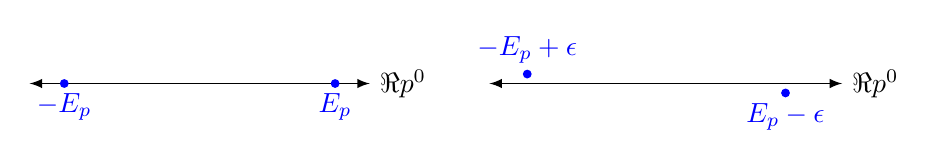
\begin{tikzpicture}[thick, scale=0.4]
    \draw[line width = 0.2mm, black, <->, >=latex] (-12.3,-2.6)--(-1.5,-2.6) node[right]{$\Re p^0$};
    \filldraw[blue](-11.2,-2.6)circle(2.9pt) node[below, blue] {$-E_p$};
    \filldraw[blue](-2.6,-2.6)circle(2.9pt) node[below, blue] {$E_p$};
    \draw[line width = 0.2mm, black, <->, >=latex] (2.3,-2.6)--(13.5,-2.6) node[right]{$\Re p^0$};
    \filldraw[blue](3.5,-2.3)circle(2.9pt) node[above, blue] {$-E_p+\ii \epsilon$};
    \filldraw[blue](11.7,-2.9)circle(2.9pt) node[below, blue] {$E_p-\ii \epsilon$};
    \end{tikzpicture}
    \caption{Cambio infinitesimal en la posición de los polos.}
    \label{fig_3.1}
\end{figure}

Cambiando infinitesimalmente la posición de los polos del eje real como se indica en la figura (\ref{fig_3.1}), es posible replantear la forma de $G(p)$ presente en la integral (\ref{eq_3.118}). Vamos a determinar dichos polos, entonces partimos de la prescripción propuesta por Feynman la cual modifica la ecuación (\ref{eq_3.117}) introduciendo un parámetro $\epsilon^\prime \to 0$,

\newcommand{\pf}{\Delta_F}
\begin{equation}
    \pf(p) = \frac{1}{p^2 - m^2 + \ii \epsilon^\prime},
    \label{eq_3.119}
\end{equation}
donde los ceros en el denominador (polos) se hallan de la siguiente manera:

\begin{prof}
	
	\begin{IEEEeqnarray*}{rCl}
		p^2-m^2 + \ii \epsilon^\prime &=& \qty(p^0)^2 - \qty( \vb*{p}^2+m^2 ) + \ii \epsilon^\prime = \qty(p^0)^2 - E_p^2 + \ii \epsilon^\prime = 0\\
		&& \implies \qty(p^0)^2 =  E_p^2 - \ii \epsilon^\prime\\
		&& \implies p^0 = \pm \sqrt{E_p^2 - \ii \epsilon^\prime} = \pm E_p \sqrt{1 - \ii \frac{\epsilon^\prime}{E_p^2}} \approx \pm E_p\qty( 1 - \frac{\epsilon^\prime}{2E_p^2}) ,
	\end{IEEEeqnarray*}
	
	de manera que ahora los polos de la integral (\ref{eq_3.118}) en $p^0$ están en el plano complejo en los puntos
	\begin{equation}
		p^0 = \pm (E_p - \ii \epsilon), \quad \quad  \epsilon \equiv \frac{\epsilon^\prime}{2E_p} 
	\end{equation}
	lo que nos permite escribir el denominador de (\ref{eq_3.119}) como
	
	\begin{equation*}
		\begin{split}
			\qty\big(p^0+\qty(E_p - \ii \epsilon))\qty\big(p^0 - \qty(E_p - \ii \epsilon)) &= \qty\big(\qty(p^0)^2 - \qty(E_p - \ii \epsilon)^2) \\
			&= \qty(p^0)^2 - E_p^2 + 2\ii E_p \epsilon + \underbrace{\epsilon^2}_{\approx 0}\\
			&= \qty(p^0)^2 - E_p^2  + \ii \epsilon^\prime.
		\end{split}
	\end{equation*}
	
	Hemos demostrado entonces que la ecuación (\ref{eq_3.119}) puede escribirse como
	
	\begin{equation}
		\begin{split}
			\pf (p) &= \frac{1}{\qty\big(p^0+\qty(E_p - \ii \epsilon))\qty\big(p^0-\qty(E_p - \ii \epsilon))}\\
			&=\frac{1}{2E_p} \qty[ \frac{1}{p^0-\qty(E_p - \ii \epsilon)} - \frac{1}{p^0+\qty(E_p - \ii \epsilon)} ] 
		\end{split}
	\end{equation}
	donde se ha expresado el resultado aplicando fracciones parciales. Con esto ya podemos replantear la integral (\ref{eq_3.118}) asociada a la función de Green $G\qty(x-x^\prime) \equiv \Delta_F \qty(x-x^\prime)$ como siendo
	
	\begin{IEEEeqnarray}{rCl}
		\pf \qty(x-x^\prime) &=& \int \frac{\dd[4]{p}}{\qty(2\pi)^4} \frac{\ee^{- \ii p(x-x^\prime)}}{ p^2 - m^2 + \ii \epsilon^\prime } \notag \\
		&=& \int \frac{\dd[4]{p}}{\qty(2\pi)^4} \frac{\ee^{- \ii p(x-x^\prime)}}{2E_p} \qty[ \frac{1}{p^0-\qty(E_p - \ii \epsilon)} - \frac{1}{p^0+\qty(E_p - \ii \epsilon)} ]\notag \\
		&=& \int \frac{\dd[3]{p}}{\qty(2\pi)^3} \frac{\ee^{ \ii \vb*{p}\cdot(\vb*{x}-\vb*{x}^\prime)}}{2E_p} \int_{-\infty}^{\infty} \frac{\dd{p^0}} {\qty(2\pi)} \qty[ \frac{\ee^{- \ii p^0(t-t^{\prime})}}{p^0-\qty(E_p - \ii \epsilon)} - \frac{\ee^{- \ii p^0(t-t^{\prime})}}{p^0+\qty(E_p - \ii \epsilon)} ].
		\label{eq_3.122}
	\end{IEEEeqnarray}
	
\end{prof}


Para evaluar la integral (\ref{eq_3.122}) en $p^0$, aplicamos variable compleja. Para ello vamos a resolver la siguiente integral.
    
    \begin{equation}
    	\boxed{
        \int_{-\infty}^\infty \frac{\ee^{-ia \zeta }}{\zeta+ib} \dd{\zeta} }\, .
        \label{eq_3.123}
    \end{equation}

Reescribimos la integral en el plano complejo y contemplemos dos casos.


\begin{itemize} 
    \item[$i)$] Si $a<0$, el exponente de la exponencial en la integral será negativo. Veamos que sucede con su parte real,
        \begin{equation}
            \Re \qty\big(-\ii a \zeta) = \Re \qty\big(-\ii a \qty(\zeta_x + \ii \zeta_y)) =  \Re \qty\big(-\ii a \zeta_x + \zeta_y) ) = a \zeta_y,
            \label{eq_3.124}
        \end{equation}
    indicándonos que $\Re \qty\big(-\ii a \zeta)$ es positiva si $\zeta_y < 0$ y negativa si $\zeta_y > 0$.   

    \begin{minipage}[b]{0.7\textwidth}
    Por lo tanto, para evaluar (\ref{eq_3.123}) es necesario que la parte real del exponente de la exponencial sea negativa, de modo que conviene trabajar con un contorno $c$ semicircular definido en la parte positiva de $\Im \zeta$, tal como se muestra en la figura (\ref{fig_3.2}).\\
    
    Antes de evaluar la integral, para evaluarlas aplicaremos el \emph{Teorema de residuos}, el cual establece
    \end{minipage}\hfill 
    \begin{minipage}[b]{0.3\textwidth}
        \begin{figure}[H]
        \centering
        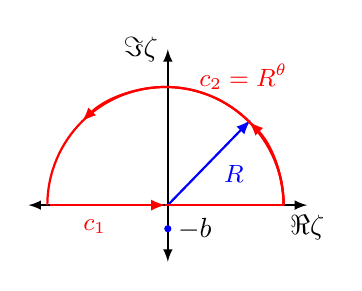
\begin{tikzpicture}[thick, scale=0.3]
            \node[below, red] at (6.8,3.8){\small $c_2 = R\ee^{\ii\theta}$};
            \node[below, red] at (0.5,-2.8){\small $c_1$};
            \node[below, blue] at (6.4,-0.5){\small{$R$}};
            \draw[line width = 0.2mm, black, <->, >=latex] (-2.3,-2.6)--(9.5,-2.6) node[below]{$\Re \zeta$};
            \draw[line width = 0.2mm, black, <->, >=latex] (3.6,-5)--(3.6,4.0) node[left]{$\Im \zeta$};
            \draw[red, ->, >=latex ](-1.4,-2.6) -- (3.5,-2.6);
            \draw[blue, ->, >=latex ](3.6,-2.6) -- (7.1,1.0);
            \draw[red](3.5,-2.6) -- (8.5,-2.6);
            \draw[red] (8.5,-2.6) arc (0:180:5);
            \draw[red, ->, >=latex] (8.5,-2.6) arc (0:45:5);
            \draw[red, ->, >=latex] (8.5,-2.6) arc (0:135:5);
            \filldraw[blue](3.6,-3.6)circle(2.9pt) node[right, black] {$-\ii b$};
        \end{tikzpicture}
        \caption{\small{Curva $c$.}}
        \label{fig_3.2}
        \end{figure}
    \end{minipage}

    \begin{theorem} [Teorema de la curva de Cauchy]
        Si $f(z)$ es una función holomorfa, la integral sobre un contorno $c$ (no importa la forma) que encierra un punto singular $z_0$ es
            \begin{equation}
                \oint_{c} f(z) dz = 2\pi \ii \Res_{z_0} \qty(f(z)), 
            \end{equation} 
        siendo $\Res_{z_0}(f(z))$, el residuo de la función en el punto $z_0$. Si $z_0$ es un polo de orden $n$, la expresión para calcular el residuo es 
            \begin{equation}
                \Res_{z_0}(f(z))=\frac{1}{(n-1)!} \lim_{z\to z_0} \frac{d^{n-1}}{dz^{n-1}}\qty\big(\qty(z-z_0)^n f(z)).
            \end{equation}
        Si el contorno no encierra ninguna singularidad, la integral sobre este es cero.
    \end{theorem}

    Entonces podemos escribir la integral (\ref{eq_3.123}) como

    \begin{equation}
        \oint_{c} \frac{\ee^{-\ii a \zeta}}{z+\ii b} \dd{\zeta} = \int_{c_1} \frac{\ee^{-\ii a \zeta}}{\zeta+\ii b} \dd{\zeta} + \int_{c_2} \frac{\ee^{-\ii a \zeta}}{\zeta+\ii b} \dd{\zeta} = 0.
        \label{eq_3.127}
    \end{equation}
    Al evaluar la integral sobre $c_2$,
    \begin{equation*}
        \begin{split}
            \int_{c_2}  \frac{\ee^{-\ii a \zeta}}{z+\ii b} \dd{\zeta} &= \ii \lim_{R \to \infty} \int_0^\pi \dd{\theta} R\ee^{\ii \theta} \frac{\ee^{-\ii a R \ee^{\ii \theta}}}{R \ee^{\ii \theta}+\ii b} \approx \ii \lim_{R \to \infty} \int_0^\pi \dd{\theta} R\ee^{\ii \theta} \frac{\ee^{-\ii a R \ee^{\ii \theta}}}{R \ee^{\ii \theta}} \\
            &= \ii \lim_{R \to \infty} \int_0^\pi \dd{\theta} \ee^{-\ii a R \cos \theta }\ee^{a R \sin \theta } \to 0, 
        \end{split}
    \end{equation*}
    donde se ha considerado el hecho que $a<0$ en el límite cuando $R\to \infty$ para el termino $\ee^{a R \sin \theta }$, además la cantidad $\ee^{-ia R \cos \theta }$ siempre será acotada aun cuando consideremos el límite al infinito.\\

    Entonces, la integral (\ref{eq_3.127}) se reduce solo sobre el eje real ($c_1$) y resulta
    \begin{equation}
        \int_{-\infty}^\infty \frac{\ee^{-\ii a \zeta}}{\zeta+\ii b} \dd{\zeta} = 0.
        \label{eq_3.128}
    \end{equation} 
    
    \begin{minipage}[b]{0.7\textwidth}
    \item[$ii)$] Si $a>0$, la ecuación (\ref{eq_3.124}) nos indica que $\Re \qty\big(-\ii a \zeta)$ es positiva si $\zeta_y > 0$ y negativa si $\zeta_y < 0$.\\
    
    En consecuencia, conviene trabajar con un contorno semicircular definido en la parte negativa del eje imaginario $\Im \zeta$ como se muestra en la figura (\ref{fig_3.3}). Así se garantizará que la integral sobre el arco $c_2$ al tomar el límite al infinito, decaiga a cero.\\
    \end{minipage}\hfill 
    \begin{minipage}[b]{0.3\textwidth}
        \begin{figure}[H]
        \centering
        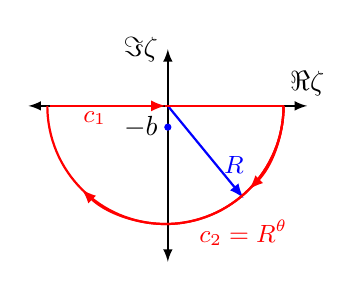
\begin{tikzpicture}[thick, scale=0.3]
            \node[below, red] at (6.8,-2.8){\small $c_2 = R\ee^{\ii\theta}$};
            \node[below, red] at (0.5,1.8){\small $c_1$};
            \node[below, blue] at (6.4,-0.1){\small{$R$}};
            \draw[line width = 0.2mm, black, <->, >=latex] (-2.3,1.6)--(9.5,1.6) node[above]{$\Re \zeta$};
            \draw[line width = 0.2mm, black, <->, >=latex] (3.6,-5)--(3.6,4.0) node[left]{$\Im \zeta$};
            \draw[red, ->, >=latex ](-1.4,1.6) -- (3.5,1.6);
            \draw[blue, ->, >=latex ](3.6,1.6) -- (6.8,-2.3);
            \draw[red](3.5,1.6) -- (8.5,1.6);
            \draw[red] (8.5,1.6) arc (0:-180:5);
            \draw[red, ->, >=latex] (8.5,1.6) arc (0:-45:5);
            \draw[red, ->, >=latex] (8.5,1.6) arc (0:-135:5);
            \filldraw[blue](3.6,0.7)circle(2.9pt) node[left, black] {$-\ii b$};
        \end{tikzpicture}
        \caption{\small{Curva $c$.}}
        \label{fig_3.3}
        \end{figure}
    \end{minipage}   

    Así,

    \begin{equation}
        \oint_c \frac{\ee^{-\ii a \zeta}}{\zeta+\ii b} \dd{\zeta} = \int_{c_1} \frac{\ee^{-\ii a \zeta}}{\zeta+\ii b} \dd{\zeta} + \int_{c_2} \frac{\ee^{-\ii a \zeta}}{\zeta+\ii b} \dd{\zeta} = - 2\pi \ii \Res_{-\ii b} \qty(\frac{\ee^{-\ii a \zeta}}{\zeta+\ii b}),
        \label{eq_3.129}
    \end{equation}
    donde el signo menos en el resultado se debe a que recorremos la trayectoria en sentido horario. El residuo de la función es 
    \begin{equation}
        \Res_{-ib} \qty(\frac{\ee^{-\ii a \zeta}}{\zeta+\ii b})=\lim_{ \zeta \to -\ii b} \cancel{\qty( \zeta + \ii b)}\frac{\ee^{-\ii a \zeta}}{\cancel{\qty(\zeta+\ii b)}} = \ee^{-ab},
    \end{equation}
    además nuevamente en el límite cuando $R\to \infty$ se tiene que 
    \begin{equation*}
        \begin{split}
            \int_{c_2} \frac{\ee^{-\ii a \zeta}}{\zeta+\ii b} \dd{\zeta} & \approx \ii \lim_{R \to \infty} \int_{2\pi}^{\pi}  \dd{\theta} R\ee^{\ii \theta} \frac{\ee^{-\ii a R \ee^{\ii \theta}}}{R \ee^{\ii \theta}}\\
            &= \ii \lim_{R \to \infty} \int_{2\pi}^{\pi}  \dd{\theta} \ee^{-\ii a R\cos \theta}\ee^{a R\sin  \theta}\to 0, 
        \end{split}
    \end{equation*}
    la cual tiende a cero por el término $\ee^{a R\sin  \theta}$ con $R\to \infty$, debido a que $\sin \theta$ es negativo en el intervalo de integración. La expresión $\ee^{-\ii a R\cos \theta}$ no afecta en el límite porque nuevamente permanece acotada en el límite. Así en (\ref{eq_3.129}) en el límite de $R$ al infinito, la integral sobre $c_1$ es

    \begin{equation}
        \int_{-\infty}^\infty \frac{\ee^{-\ii a \zeta}}{\zeta+\ii b} \dd{\zeta} = - 2\pi \ii \ee^{-ab}.
        \label{eq_3.131}
    \end{equation}
\end{itemize}
Vamos a considerar $b=\epsilon \to 0$, en la integral (\ref{eq_3.123}) pues nos será mas conveniente de esa manera. Entonces las soluciones (\ref{eq_3.128}) y (\ref{eq_3.131}) son

\begin{IEEEeqnarray*}{rCl}
    a<0 & \implies & \int_{-\infty}^\infty \frac{\ee^{-\ii a \zeta}}{\zeta+\ii \epsilon} \dd{\zeta} = 0\\
    a>0 & \implies & \int_{-\infty}^\infty \frac{\ee^{-\ii a \zeta}}{\zeta+\ii \epsilon} \dd{\zeta} = - 2\pi \ii, 
\end{IEEEeqnarray*}

que lo podemos escribir usando la función Heaviside de la forma

\begin{equation}
    \boxed{
    \int_{-\infty}^\infty  \frac{\ee^{-\ii a \zeta}}{\zeta+\ii \epsilon} \dd{\zeta}= - 2\pi \ii \Theta(a) } \, .
    \label{eq_3.132}
\end{equation}

Con este resultado, podemos evaluar cada una de las integrales de la ecuación (\ref{eq_3.122}). Comencemos con

\begin{equation*}
    I_1 \equiv \int_{-\infty}^\infty \frac{\dd{p^0}} {\qty(2\pi)} \frac{\ee^{ -\ii p^0(t-t^{\prime})}}{\qty\big(p^0-\qty(E_p - \ii \epsilon))},
\end{equation*}
la cual podemos reescribir haciendo\footnote{Las variables $p^0$ y $E_p$ no son las mismas, dado que al inicio de la sección se propuso que cada una de las componentes del cuadrivector $p^\mu$ sean independientes entre si} $p^{0 \prime}=p^0-E_p$ de modo que $dp^{0 \prime}=dp^0$, por lo tanto

\begin{IEEEeqnarray}{rCl}
    I_1 = \int_{-\infty}^\infty \frac{\dd{p^{0 \prime}}} {\qty(2\pi)} \frac{\ee^{- \ii \qty(p^{0\prime}+E_p)(t-t^{\prime})}}{\qty( p^{0 \prime} + \ii \epsilon)} &=& \ee^{- \ii E_p(t-t^{\prime})} \int_{-\infty}^\infty \frac{\dd{p^{0 \prime}}} {\qty(2\pi)} \frac{\ee^{- \ii p^{0\prime}(t-t^{\prime})}}{\qty( p^{0 \prime} + \ii \epsilon)} \notag \\
    &=&- \ii \Theta(t-t^{\prime}) \ee^{- \ii E_p(t-t^{\prime})} ,
    \label{eq_3.133}
\end{IEEEeqnarray}
donde se ha usado (\ref{eq_3.132}). Ahora evaluamos

\begin{equation*}
    I_2 \equiv \int_{-\infty}^\infty \frac{\dd{p^0}} {\qty(2\pi)} \frac{\ee^{ -\ii p^0(t-t^{\prime})}}{\qty\big(p^0+\qty(E_p - \ii \epsilon))},
\end{equation*}
donde se considera $p^{0 \prime}=-\qty(p^0+E_p)$ de modo que $dp^{0 \prime}=-dp^0$, así

\begin{IEEEeqnarray}{rCl}
    I_2 = - \int_{\infty}^{-\infty} \frac{\dd{p^{0 \prime}}} {\qty(2\pi)} \frac{\ee^{ -\ii \qty(-p^{0\prime} - E_p)(t-t^{\prime})}}{\qty( -p^{0 \prime} - \ii \epsilon)} &=& - \ee^{- \ii E_p(t^{\prime}-t)} \int_{-\infty}^\infty \frac{\dd{p^{0 \prime}}} {\qty(2\pi)} \frac{\ee^{-\ii p^{0\prime}(t^{\prime}-t)}}{\qty(p^{0 \prime} + \ii \epsilon)} \notag \\
    &=& \ii \Theta(t^{\prime}-t) \ee^{- \ii E_p(t^{\prime}-t)} .
    \label{eq_3.134}
\end{IEEEeqnarray}

Empleando (\ref{eq_3.133}) y (\ref{eq_3.134}) en el propagador (\ref{eq_3.122}),

\begin{IEEEeqnarray}{rCl}
    \pf \qty(x-x^\prime) &=& - \ii \int \frac{\dd[3]{p}}{\qty(2\pi)^3} \frac{\ee^{ \ii \vb*{p}\cdot(\vb*{x}-\vb*{x}^\prime)}}{2E_p} \qty[ \Theta(t-t^{\prime}) \ee^{- \ii E_p(t-t^{\prime})} + \Theta(t^{\prime}-t) \ee^{- \ii E_p(t^{\prime}-t)}] \notag \\
    \pf \qty(x-x^\prime) &=& - \ii \int \frac{\dd[3]{p}}{2E_p \qty(2\pi)^3} \qty[ \Theta(t-t^{\prime}) \ee^{ - \ii E_p(t-t^{\prime}) + \ii \vb*{p}\cdot(\vb*{x}-\vb*{x}^\prime)} + \Theta(t^{\prime}-t) \ee^{- \ii E_p(t^{\prime}-t)+\ii \vb*{p}\cdot(\vb*{x}-\vb*{x}^\prime)} ]. $\IEEEeqnarraynumspace$
    \label{eq_3.135}
\end{IEEEeqnarray}

Al hacer el cambio de variable $ \vb*{p^\prime}\to \vb*{-p}$ en la segunda integral,

\begin{IEEEeqnarray*}{rCl}
    $\faDribbble$ & \equiv & \int \frac{\dd[3]{p}}{2E_p \qty(2\pi)^3} \Theta(t^{\prime}-t) \ee^{- \ii E_p(t^{\prime}-t)+\ii \vb*{p}\cdot(\vb*{x}-\vb*{x}^\prime)} \\ 
    &=& (-1)^3 \int_{\infty}^{-\infty} \frac{\dd[3]{p^\prime}}{2E_{-p^\prime}} \Theta(t^{\prime}-t) \ee^{- \ii E_{-p^\prime}(t^{\prime}-t)-\ii \vb*{p}^\prime \cdot(\vb*{x}-\vb*{x}^\prime)} ,
\end{IEEEeqnarray*}
donde ya se demostró que $E_{-p}=E_p$ y los límites en las tres integrales se reajustan por el factor $(-1)^3$. Entonces cambiamos nuevamente la variable de integración $\vb*{p}^\prime \to \vb*{p}$

\begin{IEEEeqnarray}{rCl}
    $\faDribbble$ &=& \int \frac{\dd[3]{p}}{2E_{p}} \Theta(t^{\prime}-t) \ee^{\ii E_{p}(t-t^{\prime})-\ii \vb*{p}\cdot(\vb*{x}-\vb*{x}^\prime)}.
\end{IEEEeqnarray}
Con lo anterior reescribimos el propagador de Feynman (\ref{eq_3.135}),

\begin{IEEEeqnarray}{rCl}
    \ii \pf \qty(x-x^\prime) &=& \int \frac{\dd[3]{p}}{2E_p \qty(2\pi)^3} \qty[ \Theta(t-t^{\prime}) \ee^{ - \ii E_p(t-t^{\prime}) + \ii \vb*{p}\cdot(\vb*{x}-\vb*{x}^\prime)} + \Theta(t^{\prime}-t) \ee^{ \ii E_p(t-t^{\prime})-\ii \vb*{p}\cdot(\vb*{x}-\vb*{x}^\prime)} ] , \notag 
\end{IEEEeqnarray}

\begin{equation}
    \boxed{\ii \pf \qty(x-x^\prime)  = \int \frac{\dd[3]{p}}{2E_p \qty(2\pi)^3} \qty[ \Theta(t-t^{\prime}) \ee^{-\ii p(x-x^{\prime})} + \Theta(t^{\prime}-t) \ee^{\ii p(x-x^{\prime})} ] } \, .
    \label{eq_3.137}
\end{equation}

siendo ahora \emph{las componentes del cuadrivector} $p \equiv (E_p,\vb*{p})$ con $E_p=\sqrt{\vb*{p}^2+m^2}$.\\

Como ejercicio se deja demostrar que el propagador de Feynman satisface la ecuación que define la función de Green (\ref{eq_3.107})

\begin{equation}
    \qty(\square_x + m^2)\pf(x-x^\prime)=-\delta^4 (x-x^\prime). 
\end{equation}
garantizando el hecho de que es una \emph{función de Green} de la ecuación de movimiento.\\

Una ves estudiado el propagador de Feynman como una función de Green, miremos como se relaciona con la cuantización de los campos. Si analizamos solamente el campo escalar real, 

\begin{equation*}
    \Ophi \left(x\right) =  \int \frac{\dd[3]{p}}{\sqrt{2\qty(2\pi)^{3}E_p}} \qty\bigg[\Oa_p \ee^{-\ii px} + \Oa^{\dag}_p\ee^{\ii px}].
\end{equation*}

La acción de este operador sobre el estado \emph{vacio} junto con las expresiones (\ref{eq_3.57}) y (\ref{eq_3.67}) implican

\begin{IEEEeqnarray}{rCl}
    \Ophi \left(x\right) \ket{0} &=& \int \frac{\dd[3]{p}}{\sqrt{2\qty(2\pi)^{3}E_p}} \qty\bigg[ \cancelto{0}{\Oa_p \ket{0}}\ee^{-\ii px} + \Oa^{\dag}_p \ket{0} \ee^{\ii px}] \notag \\
    &=& \int \frac{\dd[3]{p}}{\sqrt{2\qty(2\pi)^{3}E_p}} \ee^{\ii px} \ket{p}.
    \label{eq_3.139}
\end{IEEEeqnarray}

Al tomar el adjunto hermítico de $\ket{p} = \Oa^\dag_p \ket{0}$, demostramos que era de la forma $\bra{p}=\bra{0}\Oa_p$. Calculando la acción del campo escalar real sobre el $\bra{0}$,

\begin{IEEEeqnarray}{rCl}
    \bra{0}\Ophi \qty(x^\prime) &=& \int \frac{\dd[3]{p^\prime}}{\sqrt{2\qty(2\pi)^{3}E_{p^\prime}}} \qty\bigg[  \bra{0}\Oa_{p^\prime} \ee^{-\ii p^\prime x^\prime} + \cancelto{0}{\bra{0} \Oa^{\dag}_{p^\prime}}\ee^{\ii p^\prime x^\prime}]\notag \\
    &=& \int \frac{\dd[3]{p^\prime}}{\sqrt{2\qty(2\pi)^{3}E_{p^\prime}}} \ee^{-\ii p^\prime x^\prime} \bra{p^\prime}.
    \label{eq_3.140}
\end{IEEEeqnarray}

Los resultados anteriores nos permiten calcular dos cosas. Lo primero es que el valor esperado del campo escalar real en el estado vacío es cero, puesto que

\begin{equation}
    \ev{\Ophi \qty(x)}{0} = \int \frac{\dd[3]{p}}{\sqrt{2\qty(2\pi)^{3}E_p}} \ee^{\ii px} \cancelto{0}{\braket{0}{p}} = 0.
\end{equation}

Y la segunda, que el valor esperado del operador $\Ophi$ elevado al cuadrado es diferente de cero. Es decir

\begin{IEEEeqnarray}{rCl}
    \ev{ \Ophi \qty(x^\prime) \Ophi \qty(x)}{0} &=& \qty(\int \frac{\dd[3]{p^\prime}}{\sqrt{2\qty(2\pi)^{3}E_{p^\prime}}} \ee^{-\ii p^\prime x^\prime} \bra{p^\prime}) \qty( \int \frac{\dd[3]{p}}{\sqrt{2\qty(2\pi)^{3}E_p}} \ee^{\ii px} \ket{p} ) \notag \\
    &=& \int \int \frac{\dd[3]{p^\prime}}{\sqrt{2\qty(2\pi)^{3}E_{p^\prime}}} \frac{\dd[3]{p}}{\sqrt{2\qty(2\pi)^{3}E_p}} \ee^{\ii \qty( px - p^\prime x^\prime) } \underbrace{\braket{p^\prime}{p}}{\delta^3(\vb*{p}^\prime-\vb*{p}) }  \, . \notag 
\end{IEEEeqnarray}

\begin{equation}
    \boxed{
    \ev{ \Ophi \qty(x^\prime) \Ophi \qty(x)}{0} = \int  \frac{\dd[3]{p}}{2\qty(2\pi)^{3}E_p} \ee^{\ii p \qty(x - x^\prime)} } \, .
    \label{eq_3.142}
\end{equation}
Análogamente podemos calcular

\begin{equation}
    \boxed{
    \ev{ \Ophi \qty(x) \Ophi \qty(x^\prime)}{0} = \int  \frac{\dd[3]{p}}{2\qty(2\pi)^{3}E_p} \ee^{\ii p \qty(x^\prime - x)} } \, .
    \label{eq_3.143}
\end{equation}

Note que en la ultima expresión si hacemos el cambio e variable $ \vb*{p} \to -\vb*{p}$, no tenemos problema con el diferencial y los limites de integración, pero el exponente se transforma en

\begin{equation*}
    p(x^\prime-x) = p_0(x^{0\prime} - x^0 ) - \vb*{p}(\vb*{x^\prime}-\vb*{x}) \quad \to \quad  p_0(x^0 - x^{0\prime}) + \vb*{p}(\vb*{x^\prime}-\vb*{x}),
\end{equation*}

es decir el exponente de las expresiones (\ref{eq_3.142}) y (\ref{eq_3.143}) no son iguales, no quedan en forma covariante y por lo tanto

\begin{equation}
    \boxed{
    \ev{ \Ophi \qty(x^\prime) \Ophi \qty(x)}{0} \neq  \ev{ \Ophi \qty(x) \Ophi \qty(x^\prime)}{0} } \, .
\end{equation}

Ahora vamos a emplear el propagador (\ref{eq_3.137}), para escribirlo en términos de los operadores de campo $\Ophi$. Reemplacemos cada una de las integrales de (\ref{eq_3.137}) por su equivalente en términos de operadores (\ref{eq_3.142}) y (\ref{eq_3.143}),

\begin{equation}
    \boxed{
    \ii \pf \qty(x-x^\prime)  = \Theta(t-t^{\prime}) \ev{ \Ophi \qty(x) \Ophi \qty(x^\prime)}{0} + \Theta(t^{\prime}-t) \ev{ \Ophi \qty(x^\prime) \Ophi \qty(x)}{0} } \, .
    \label{eq_3.145}
\end{equation}

es decir como una suma pesada de dos funciones de dos puntos. Es mas usual expresar el propagador en términos del \emph{operador de ordenamiento temporal}, es decir

\newcommand{\OrdT}{\mathcal{T}}

\begin{equation}
    \boxed{\ii \pf \qty(x-x^\prime)  = \ev{ \OrdT \qty\big[ \Ophi \qty(x) \Ophi \qty(x^\prime) ]}{0} } \, .
\end{equation}

donde $\OrdT$ para campos bosónicos está definido como

\begin{equation}
    \boxed{
    \OrdT \qty\big[ A \qty(x) B \qty(x^\prime) ] = \left\{ \,
    \begin{IEEEeqnarraybox}[][c]{l?s}
        \IEEEstrut
            A \qty(x) B \qty(x^\prime) & Si $\quad t>t^\prime$  \\
            B \qty(x^\prime) A \qty(x) & Si $\quad t<t^\prime$ 
        \IEEEstrut
    \end{IEEEeqnarraybox}
    \right.
    \label{eq_3.147}} \, .
\end{equation}

El operador $\OrdT \qty [ ... ]$ representa un producto de operadores ordenados por el tiempo, donde el operador con el tiempo posterior debe colocarse a la izquierda del operador con el tiempo anterior.\\

Interpretemos (\ref{eq_3.145}). Si $t<t^{\prime}$, solo sobrevive el segundo término asociado a $\ev{ \Ophi \qty(x^\prime) \Ophi \qty(x)}{0}$. Para entenderlo, recordemos que de (\ref{eq_3.139}) el operador $\Ophi(x)$ actuando sobre el \emph{vacío} crea una \emph{partícula} en el tiempo $t$ y con momento $\vb*{p}$. Pero, la acción del operador $\Ophi(x^\prime)$ sobre el $\bra{0}$ en (\ref{eq_3.140}) se caracteriza porque solo contribuye la parte asociada al operador destrucción, y por tanto lo podemos interpretar como la destrucción de una partícula en un tiempo $t^\prime$. En conclusión el elemento de matriz $\ev{ \Ophi \qty(x^\prime) \Ophi \qty(x)}{0}$ describe la \emph{amplitud de una partícula} que se crea en el tiempo $t$, se propaga en el espacio-tiempo y se destruye en un tiempo posterior $t^\prime$.\\

De la misma manera, si $t > t^\prime $ solo sobrevive el primer término de (\ref{eq_3.145}) asociado al elemento de matriz $\ev{ \Ophi \qty(x) \Ophi \qty(x^\prime)}{0}$, el cual describe la amplitud de una partícula que se crea en el tiempo $t^\prime$, se propaga en el espacio tiempo y se destruye en el tiempo posterior $t$. Esto es el sentido físico del propagador, elemento importante para calcular las amplitudes de varios procesos que involucran interacciones de partículas.

\section{Adicional: Interpretación de partícula y función de n Puntos}

\subsection{Interpretación de Partícula}

En la sección \ref{Efockes} comentamos que los estados construidos a partir de actuar con $n$ operadores de creación sobre el vacío podían considerarse como estados de $n$ partículas con momentos definidos (\emph{multipartículas}). Vamos a ver, siguiendo un ejercicio, que los estados dados por $\Ophi(t,\vb*{x})\ket{0} $ describen lo más cercano que uno puede tener a la noción de partícula localizada en un punto del espacio $\vb*{x}$ a tiempo $t$.\\

Vamos a analizar en qué medida la teoría del campo escalar real libre, restringida a los estados de una partícula, puede ser considerada como una generalización relativista de la teoría de Schrödinger, y como el operador $\Ophi(x)$ puede ser asimilado a un operador de creación de una partícula en un punto del espacio. Primero vamos a mostrar que los vectores $\Ophi(x)=\Ophi(t,\vb*{x})$ a un tiempo fijo generan todo el espacio de Hilbert $\mathscr{H}_1$ de una partícula.\\

Para simplificar el desarrollo, tomamos el tiempo fijo $t=0$ (el resultado no cambia). Lo que se pretende ver en este inciso es que haciendo combinaciones lineales de los estados dados por $\hat{\phi}(0, \vb*{x})\ket{0}$ podemos generarnos un estado de una partícula con una distribución arbitraria de momentos. Es decir, queremos ver que podemos fabricarnos un estado de la forma

\begin{equation}
    \int \frac{\dd[3]{p}}{\sqrt{2E_p(2 \pi)^3}} c(\vb*{p})\ket{\vb*{p}},
    \label{eq_3.148}
\end{equation}

donde $\ket{\vb*{p}} \equiv \hat{a}_{\vb*{p}}^{\dagger}|0\rangle$ y $c(\vb*{p})$ es una función arbitraria (que es la que determina la distribución de momentos del estado). Mantuvimos el factor $\sqrt{2 (2 \pi)^{3} {E_p}}$ al hacer la combinación lineal, pero podrían absorberse en la definición de $c(\vb*{p})$ (lo que importa es que estamos haciendo una combinación lineal).\\

Veamos qué forma tiene el estado $\hat{\phi}(0,\vb*{x})\ket{0}$. Recordando la expresión (\ref{eq_3.139}) para $t=0$, tenemos

\begin{equation}
    \hat{\phi}(0, \vb*{x})|0\rangle=\int \frac{\dd[3]{p}}{ \sqrt{2 (2 \pi)^{3} E_p}} \ee^{-\ii \vb*{p} \cdot \vb*{x}}\ket{\vb*{p}}.
\end{equation}

Ya que $\hat{a}_{p}\ket{0}=0$ y $\hat{a}_{p}^{\dagger}\ket{0}=\ket{\vb*{p}}$. Una combinación lineal arbitraria de estos estados, con coeficientes $f(\vb*{x})$, tendrá entonces la forma

\begin{equation}
    \int \dd[3]{x} f(\vb*{x}) \Ophi(0,\vb*{x})\ket{0} = \int \frac{\dd[3]{p}}{\sqrt{2\qty(2\pi)^3 E_p}}\qty[\int \dd[3]{x} f(\vb*{x})\ee^{-\ii \vb*{p} \cdot \vb*{x}}] \ket{\vb*{p}},
    \label{eq_3.150}
\end{equation}

Para conseguir un estado de la forma (\ref{eq_3.148}) necesitamos que el término entre corchetes en (\ref{eq_3.150}) sea igual a $c(\vb*{p})$. Esto se puede conseguir sencillamente tomando a $c(\vb*{p})$ como la transformada de Fourier de $f(\vb*{x})$.

Vimos entonces que una combinación lineal de estados $\hat{\phi}(0, \vb*{x})\ket{0}$ generan el espacio de Hilbert $\mathscr{H}_1$ asociado a una partícula en  un tiempo fijo $t$ .\\

Se define el estado $\ket{t,\vb*{x}}$ (\emph{Supuestos vectores de una partícula localizados}) y la función de onda $\psi \qty(t,\vb*{x}) \equiv \braket{t,\vb*{x}}{\psi}$, con $\ket{\psi} \in \mathscr{H}_1$ (\emph{Supuesta función de onda correspondiente a una partícula}). Vamos a probar que $\psi \qty(t,\vb*{x})$ satisface la ecuación KG. Además se demostrará que satisface la ecuación diferencial de primer orden en derivadas temporales

\begin{IEEEeqnarray}{rCl}
	\ii \pdv{\psi (t,\vb*{x})}{t} = + \sqrt{m^2 - \laplacian } \psi(t,\vb*{x}),
	\label{eq_3.151}
\end{IEEEeqnarray}

Para demostrar que satisface la ecuación de Klein-Gordon es sencillo ya que el mismo campo $\Ophi$ la satisface, en efecto

\newcommand{\OKG}{\qty( \square + m^2 )}

\begin{IEEEeqnarray}{rCl}
	\OKG \psi(t,\vb*{x}) & = & \OKG	 \braket{t,\vb*{x}}{\psi} \notag \\
	&=& \OKG \bra{0} \Ophi(t,\vb*{x}) \ket{\psi} \notag \\
	&=& \bra{0} \OKG  \Ophi(t,\vb*{x}) \ket{\psi} = 0,
\end{IEEEeqnarray}

donde usamos que el campo es real (y por lo tanto es igual a su conjugado) y que cumple la ecuación de Klein-Gordon (\ref{eq_3.6}).

Adicionalmente vamos a demostrar que $\psi(t,\vb*{x})$ evoluciona solo con frecuencias positivas, es decir como el operador $\Oa_p$.  Esto también es sencillo  ver, ya que los operadores $\Oa^\dag_p$ aniquilan al vacío al actuar a la izquierda.

\begin{IEEEeqnarray}{rCl}
	\psi\qty(t,\vb*{x}) &=& \braket{t,\vb*{x}}{\psi} = \bra{0} \Ophi\qty(t,\vb*{x}) \ket{\psi} \notag \\
	& = &  \int \frac{\dd[3]{p}}{\sqrt{2\qty(2\pi)^{3}E_p}} \bra{0} \qty\bigg[\Oa_p \ee^{-\ii E_p t}\ee^{\ii \vb*{p} \cdot \vb*{x}} + \Oa^{\dag}_p\ee^{\ii E_p t}\ee^{-\ii \vb*{p} \cdot \vb*{x}}] \ket{\psi} \notag \\
	& = &  \int \frac{\dd[3]{p}}{\sqrt{2\qty(2\pi)^{3}E_p}}  \ee^{\ii \vb*{p} \cdot \vb*{x}} \bra{0} \Oa_p \ket{\psi} \ee^{-\ii E_p t},
\end{IEEEeqnarray}

noten que el operador $\sqrt{m^2 - \laplacian}$ esta bien definido ya que $\qty(m^2-\laplacian)$ es positivo, hecho que se puede ver calculando 

\begin{equation}
	\qty(m^2-\laplacian ) \psi(t,\vb*{x}) =   \qty(m^2 + \vb*{p}^2) \psi(t,\vb*{x})  = E_p^2 \psi(t,\vb*{x})~.
	\label{eq_3.154}
\end{equation}

Por otro lado, para ver que se cumple la ecuación (\ref{eq_3.151}) calculemos

\begin{equation}
	\ii \pdv{\psi (t,\vb*{x})}{t} = \ii \pdv{t} \int \frac{\dd[3]{p}}{\sqrt{2\qty(2\pi)^{3}E_p}}  \ee^{\ii \vb*{p} \cdot \vb*{x}} \bra{0} \Oa_p \ket{\psi} \ee^{-\ii E_p t} = E_p \psi (t,\vb*{x}),
\end{equation}
 
 y de (\ref{eq_3.154}) resulta que
 
  
 \begin{equation}
 	\ii \pdv{\psi (t,\vb*{x})}{t} = + \sqrt{m^2 - \laplacian } \psi (t,\vb*{x}). 
 \end{equation}
 
 Se deja a modo de ejercicio verificar que la corriente conservada de Klein-Gordon da lugar a una probabilidad conservada y positiva, pero la densidad de probabilidad no es definida positiva.\\
 
 Ahora, vamos a mostrar que el valor de $\braket{x}{y} \equiv \braket{t,\vb*{x}}{t,\vb*{y}}$ no es proporcional a la función delta de Dirac y que los estados $\ket{t,\vb*{x}}$ están localizados en un tamaño típico $\Delta x \thicksim 1/m $ (\emph{en unidades naturales corresponde a la Longitud de Compton} $\frac{\hbar}{mc} $ ).\\
 
 Si bien es cierto, en mecánica cuántica no relativista, los estados de una partícula localizada en puntos distintos del espacio son ortonormales, sin embargo, aquí no ocurre eso para los estados $\ket{x}$. Calculemos
 
 \begin{IEEEeqnarray}{rCl}
 	\braket{t,\vb*{x}}{t,\vb*{y}} & = & \ev{\Ophi(t,\vb*{x})\Ophi(t,\vb*{y})}{0} \notag \\
 	& = &  \int \frac{\dd[3]{p}}{\sqrt{2\qty(2\pi)^{3}E_p}} \int \frac{\dd[3]{p^\prime}}{\sqrt{2\qty(2\pi)^{3}E_{p^\prime}}} \ee^{-\ii \qty( E_p - E_p^{\prime}) t}\ee^{\ii \qty(\vb*{p} \cdot \vb*{x} - \vb*{p}^\prime \cdot \vb*{y} )}  \ev{\Oa_p \Oa_{p^\prime}^\dag}{0}  \notag \\
 	& = &  \int \frac{\dd[3]{p}}{\sqrt{2\qty(2\pi)^{3}E_p}} \int \frac{\dd[3]{p^\prime}}{\sqrt{2\qty(2\pi)^{3}E_{p^\prime}}} \ee^{-\ii \qty( E_p - E_p^{\prime}) t}\ee^{\ii \qty(\vb*{p} \cdot \vb*{x} - \vb*{p}^\prime \cdot \vb*{y} )} \delta^3 \qty(\vb*{p}-\vb*{p}^\prime) \notag \\
 	& = & \int \frac{\dd[3]{p}}{2\qty(2\pi)^{3}E_p} \ee^{\ii \vb*{p} \cdot  \qty( \vb*{x}  - \vb*{y} )} = \int \frac{\dd[3]{p}}{2\qty(2\pi)^{3}}  \frac{\ee^{\ii \vb*{p} \cdot  \qty( \vb*{x}  - \vb*{y} )} }{(\vb*{p}^2+m^2)}.
 \end{IEEEeqnarray}
 
 Para evaluar esta integral empleamos coordenadas esféricas $\qty(p,\varphi,\theta )$ considerando el ángulo azimutal $\theta$ como el ángulo entre los vectores $\vb*{p}$ y $(\vb*{x}-\vb*{y})$. Definiendo $u \equiv \abs{\vb*{x}-\vb*{y}}$,
 
 \begin{IEEEeqnarray*}{rCl}
 	\braket{t,\vb*{x}}{t,\vb*{y}} & = & \frac{1}{2 \qty(2\pi)^3} \int_{0}^{+\infty} \dd{p} p^2  \int_{0}^{2\pi} \dd{\varphi}  \int_{-1}^{1} \dd{(\cos \theta)} \frac{\ee^{\ii p u \cos \theta}}{\sqrt{p^2 + m^2}} \\
 	& = & \frac{1}{2 \qty(2\pi)^2} \int_{0}^{+\infty} \dd{p}  \frac{p^2}{\sqrt{p^2 + m^2}}  \int_{-1}^{1} \dd{(\cos \theta)} \ee^{\ii p u \cos \theta}\\
 	& = & \frac{1}{2 \qty(2\pi)^2} \int_{0}^{+\infty} \dd{p}  \frac{p^2}{\sqrt{p^2 + m^2}} \frac{2 \sin (pu)}{pu}\\
 	& = & \frac{1}{\qty(2\pi)^2} \int_{0}^{+\infty} \dd{p}  \frac{p \sin (pu)}{u \sqrt{p^2 + m^2}}
 \end{IEEEeqnarray*}
 
 La integral anterior puede escribirse en términos de funciones de Bessel modificadas. Para llevarla a una representación integral conocida de estas funciones hay que hacer el
 cambio de variables $p = m \sinh(\alpha)$  (verifique que con ese cambio de variables resulta $dp = \sqrt{p^2 + m^2} d\alpha$)
 
 \begin{IEEEeqnarray}{rCl}
 	\braket{t,\vb*{x}}{t,\vb*{y}} & = &  \frac{m}{(2\pi)^2 u} \int_{0}^{+\infty} \dd{\alpha} \sinh(\alpha) \sin\qty\big ( mu\sinh (\alpha) ) ,
 \end{IEEEeqnarray}
 
donde el integrando que aparece en la expresión anterior es una expresión integral de la función de Bessel $ K_1 (mu)$  (ver por ejemplo la ecuación $(10.32.7)$ en \url{https://dlmf.nist.gov/10.32}) . Recordando que $ u = \abs{\vb*{x} - \vb*{y}} $ nos queda finalmente
 
 \begin{equation}
	\braket{t,\vb*{x}}{t,\vb*{y}} = \frac{1}{(2\pi)^2} \frac{m}{\abs{\vb*{x}-\vb*{y}}} K_1 \qty( m\abs{\vb*{x}-\vb*{y}} ).	
 \end{equation}

La función de Bessel $K_1$ diverge en el origen, tiende a cero en $+ \infty$ y es decreciente para todo real positivo , pero no se anula si $\abs{\vb*{x} - \vb*{y}} \neq 0$, por mas pequeña que sea esta diferencia. En particular no se anula para $\abs{\vb*{x} - \vb*{y}} \thicksim 1/m $, que restaurando unidades es la longitud de Compton. Esto nos dice que los estados no son ortogonales (algo que sí sucede en el límite no relativista, si consideramos $c$ al infinito).\\

El resultado de este ejercicio ejemplifica la dificultad de definir la noción de \textbf{localización} en una teoría relativista.\\

\subsection{Funciones de n puntos} 

Una \textbf{función de n puntos} (o \textbf{función de correlación}  o simplemente \textbf{correlador}) es un valor de expectación en vacío de $ n $ campos

\begin{equation}
	C(x_1,x_2,\ldots ,x_n) = \ev{\Ophi(x_1)\Ophi(x_2)\ldots \Ophi(x_n)}{0},
\end{equation}

Estas funciones son muy importantes ya que se relacionan con otros objetos centrales de la teoría, como los propagadores. Además, están conectadas con las amplitudes de scattering a través de la fórmula de reducción LSZ, como veremos más adelante. Desde el punto de vista axiomático, dar el conjunto completo de las funciones de correlación determina completamente la teoría de campos (esto se conoce como Teorema de Reconstrucción de Wightman).\\

Al final del ejercicio que hicimos en la sección anterior vimos un ejemplo de una función de correlación (la función de 2 puntos) a tiempos iguales

\begin{equation}
	\ev{\Ophi(t,\vb*{x})\Ophi(t,\vb*{y})}{0} = \frac{1}{(2\pi)^2} \frac{m}{\abs{\vb*{x}-\vb*{y}}} K_1 \qty( m\abs{\vb*{x}-\vb*{y}} ),
	\label{eq_3.161}
\end{equation}

 Note que si en la expresión anterior toman el límite de masa cero (consultar la expansión de $ K_1 $), se obtiene que la función de dos puntos para el campo escalar no masivo decae como $1/\abs{\qty(\vb*{x}-\vb*{y})}$.  Cuando la masa es distinta de cero, para distancias grandes, $ K_1 $ tiene un decaimiento exponencial, con lo que las correlaciones decaen más rápidamente cuando los campos son masivos.\\
 
 Otra cosa que se puede notar de la expresión (\ref{eq_3.161}) es que no depende de $ x $ e $ y $ por separado, sino que es función del módulo de su diferencia. Esto podría hacernos sospechar que es invariante ante traslaciones y también de su módulo, lo que nos hace intuir que también es invariante ante rotaciones. De los boosts podemos decir poco porque estamos mirando un ejemplo de una función de dos puntos a tiempos iguales, pero también será invariante ante boosts. En general, \emph{las funciones de correlación son invariantes ante transformaciones del grupo de Poincaré}.
 
 
 
  
%----------------------------------------------------------------------------------------

%----------------------------------------------------------------------------------------
%	CHAPTER 4
%----------------------------------------------------------------------------------------
%	CHAPTER 4 Cuantización de Campo de Dirac
%----------------------------------------------------------------------------------------

\chapterimage{chapter_head_4.pdf}

\chapter{Campos Fermiónicos} 

\label{capitulo_4}

Hasta ahora solo se ha trabajado la cuantización del campo escalar real y complejo, los cuales eran invariantes ante transformaciones del grupo de Lorentz. Los campos escalares se encargan de describir partículas que tienen espín entero. Ahora, nos concentraremos en el análisis de campos de Dirac, los cuales describen partículas de espín $1/2$.

\section{Hamiltoniano de Dirac}

En el capitulo anterior se trato de buscar la interpretación a la solución negativa de la ecuación de Klein-Gordon, hecho que permitió entender y darle un significado físico en el campo escalar tanto real, como complejo. Sin embargo, Dirac intentó darle un significado alternativo a este problema y es así como se explica el comportamiento de partículas con espín sementero. Para entender esto partimos nuevamente de la mecánica cuántica no relativista donde la ecuación de Schrödinger en la representación de las coordenadas se obtiene por reemplazar por operadores la energía y el momento, 

\begin{equation}
	\begin{split}
		E &\implies \hat{E} = \ii \pdv{t}\\
		\vb*{p} & \implies \hat{\vb*{p}} = - \ii \grad,
	\end{split}
	\label{eq_4.1}
\end{equation}
en la ecuación de autovalores 

\begin{equation}
	\OH \psi = E \psi. 
	\label{eq_4.2}
\end{equation}

En el repaso de relatividad especial, se ha definido el cuadrivector momento 

\begin{equation}
	p^\mu = \qty\big(E,\vb*{p}),
\end{equation}
el cual satisface la siguiente propiedad (en unidades naturales)

\begin{equation}
	p^\mu p_\mu = E^2 - \vb*{p}^2 = m^2.
	\label{eq_4.4}
\end{equation}

Al exigir que la energía relativista sea positiva se deberá cumplir 

\begin{equation}
	E = \qty\big( \vb*{p}^2 + m^2 )^{1/2}.
	\label{eq_4.5}
\end{equation}

La ecuación de autovalores asociada al autovector $\psi$ se puede determinar usando en (\ref{eq_4.5}) las reglas de cuantización (\ref{eq_4.1}), de tal manera que se obtiene

\begin{IEEEeqnarray}{C}
	\hat{E} \psi = \qty\big( \vb*{\Op}^2 + m^2 )^{1/2} \psi ,
	\label{eq_4.6}
\end{IEEEeqnarray} 

donde es posible expandir el RHS de tal forma que $\qty\big( \vb*{\Op}^2 + m^2 )^{1/2} \psi = m \qty\bigg[ 1 + \frac{\Op^2}{2m^2} - \frac{\Op^4}{8m^4} + \cdots ]\psi$, lo que implica conocer las derivadas de orden superior de la función de onda $\psi$. Es aquí donde Dirac propone una manera de evitar este tipo de dificultades buscando la forma de linealizar la ecuación (\ref{eq_4.5}). Una manera de lograr esto es proponiendo la existencia de un operador $D$, para ello reescribimos (\ref{eq_4.6}) en la representación de las coordenadas como:

\begin{equation}
	\ii \pdv{\psi}{t} = \qty( -\laplacian + m^2 )^{1/2} \psi ,
	\label{eq_4.7}
\end{equation}
donde se propone que 
\newcommand{\OD}{D}

\begin{equation}
	\boxed{
	\OD^2 = \Op^2 = -\qty( \pdv{t} )^2 + \laplacian, }
\end{equation}

que implica reescribir (\ref{eq_4.7}) como,

\begin{IEEEeqnarray}{rCl}
	\qty( \ii \pdv{t} )^2 = - \laplacian+m^2 \implies  && -\qty(  \pdv{t} )^2 + \laplacian = m^2 \implies \hat{D}^2 = m^2,
	\label{eq_4.8}
\end{IEEEeqnarray}

lo que verifica satisfactoriamente la ecuación (\ref{eq_4.4}). Si se propone la linealización de la ecuación de Dirac a través de

\begin{equation}
	\boxed{
		D \equiv \gamma^\mu p_\mu,}
		\label{eq_4.9}
\end{equation}

se debe cumplir (\ref{eq_4.8}), de manera que 

\begin{IEEEeqnarray*}{rCl}
	D^2 &=& \gamma^\mu \gamma^\nu p_\mu p_\nu\\
	&=& \frac{1}{2} \qty\big( \gamma^\mu \gamma^\nu + \gamma^\nu \gamma^\mu )p_\mu p_\nu\\
	&=& p^2.
\end{IEEEeqnarray*}
 identidad que se garantiza solamente si 
 
 \begin{equation}
 	\boxed{
 	\qty{\gamma^\mu ,\gamma^\nu} =\gamma^\mu \gamma^\nu + \gamma^\nu \gamma^\mu = 2 g^{\mu \nu} } \, .
 	\label{eq_4.11}
 \end{equation}

El anticonmutador obtenido obtenido anteriormente representa $16$ ecuaciones, debido a la dimensión de la métrica de Minkowski. Esta condición garantiza que la dimensión de las matrices gamma sea $4$. En la literatura $\gamma^\mu$ representan las matrices \textbf{gamma de Dirac} y la ecuación (\ref{eq_4.11}) implica que las ($\gamma^{\mu \prime}$s) satisfacen el \textbf{álgebra de Clifford}.\\

A partir de (\ref{eq_4.11}) se deducen dos propiedades importantes,

\begin{theorem}[Propiedad 1] \label{Theorem_prop1}
	Mostrar que $(\gamma^0)^2 = 1$ y $ (\gamma^i)^2 = -1$.\\
	\emph{Demostración}\\
	Partimos de la propiedad de anticonmutación de las matrices gamma (\ref{eq_4.11}) y consideramos $\mu=\nu=0$
	
	\begin{IEEEeqnarray}{rCl}
		2 \gamma^0 \gamma^0 = 2g^{00} \implies \qty(\gamma^0)^2 = 1, \IEEEyessubnumber
		\label{eq_4.11a}
	\end{IEEEeqnarray}
	
	luego, consideramos $\mu=\nu=i$, entonces
	\begin{IEEEeqnarray}{rCl+x*}
		2 \gamma^i \gamma^i= 2g^{ii} \implies \qty(\gamma^i)^2 = -1. \IEEEyessubnumber   \\ &&& \nonumber\IEEEQEDhere
		\label{eq_4.11b}
	\end{IEEEeqnarray}
\end{theorem}

\begin{theorem}[Propiedad 2]
	Si $\mu\neq \nu$ entonces las matrices gamma anticonmutan.\\
	\emph{Demostración}\\
	Partimos nuevamente de la propiedad de anticonmutación de las matrices gamma (\ref{eq_4.11}) y consideramos $\mu\neq \nu$, entonces
	\begin{IEEEeqnarray}{rCl+x*}
		\qty{\gamma^\mu,\gamma^\nu} &=& 2g^{\mu\nu}, \qquad \text{si} \quad (\mu\neq \nu) \implies g^{\mu\nu} = 0  \notag \\
		&\therefore& \qty{\gamma^\mu,\gamma^\nu} = 0 ,   \IEEEyessubnumber   \\ &&& \nonumber\IEEEQEDhere
		\label{eq_4.11c}
	\end{IEEEeqnarray}
	ecuación conocida como la relación de anticonmutación de las matrices gamma si $ \mu\neq \nu $.
\end{theorem}

Con las propiedades anteriores y la definición del operador $D$ podemos reescribir el Hamiltoniano como (ya se corrobora este resultado más adelante)

\begin{equation}
	  \boxed{
	H=\gamma^0\qty( \vb*{\gamma}\cdot \vb*{p} + \gamma^0 m ).}
	\label{eq_4.12}
\end{equation}

 \subsection{Propiedades de las matrices Gamma}
 
 Vamos a demostrar una serie de propiedades asociadas a las matrices gamma y con las cuales podremos realizar cálculos de manera mas rápida y eficiente.
 
 \begin{theorem}[Propiedad Cíclica de las trazas]
 	Sean $A$ y $B$ dos matrices de dimensión $n$, entonces 
 	\begin{IEEEeqnarray}{rCl}
 		\Tr(AB) & = & \Tr(BA). \IEEEyesnumber
 		\IEEEyessubnumber
 		\label{eq_4.13a}
 	\end{IEEEeqnarray}
 	\emph{Demostración}\\
 	Partimos del lado izquierdo de la ecuación (\ref{eq_4.13a}),
 	
 	\begin{IEEEeqnarray*}{rCl+x*}
 		\Tr(AB) = (AB)_{ii}  =A_{ij} B_{ji} = B_{ji} A_{ij} = (BA)_{jj} = \Tr(BA).    \\ &&& \nonumber\IEEEQEDhere
 	\end{IEEEeqnarray*}
 	
  De aquí es obvio que 
  \begin{IEEEeqnarray}{rCl}
  	\Tr( A_1 A_2 A_3 ) & = & \Tr( A_2 A_3 A_1 ) = \Tr( A_3 A_1 A_2). \IEEEyessubnumber
  \end{IEEEeqnarray}
  	Con este resultado podemos generalizar para $k$ matrices que  
  	\begin{IEEEeqnarray}{rCl}
  	\Tr( A_1 A_2 \ldots A_k ) & = & \Tr( A_2 A_3 \ldots A_k A_1 ). \IEEEyessubnumber
  	\label{eq_4.24c}
  \end{IEEEeqnarray}
\end{theorem}

\vspace{2cm}
\begin{theorem}[Propiedad 3 - Traza de las matrices gamma]
	La traza de cada una de las matrices gamma es cero.\\
	\begin{IEEEeqnarray}{rCl}
		\Tr(\gamma^\mu) = 0 \quad \forall ~ \mu. \IEEEyessubnumber
		\label{eq_4.13d}
	\end{IEEEeqnarray}
	\emph{Demostración}\\
	Partimos nuevamente de la propiedad de las matrices gamma (\ref{eq_4.11}) y consideramos $\mu = \nu$, entonces
	
	\begin{IEEEeqnarray*}{rCl}
		2\gamma^\mu \gamma^\mu &=& 2 g^{\mu \mu}  \implies \frac{\gamma^\mu \gamma^\mu }{g^{\mu \mu}} = 1,
	\end{IEEEeqnarray*}
	
	donde $g^{\mu \mu}$ representa un número (elemento de la diagonal principal de la métrica) y $1$ representa la matriz identidad. Ahora si multiplicamos el resultado anterior por $\gamma^\nu$,
	\begin{IEEEeqnarray*}{rCl's}
		\gamma^\nu = \frac{\gamma^\nu \gamma^\mu \gamma^\mu }{g^{\mu \mu}}  &&\implies \Tr(\gamma^\nu) = \Tr(\frac{\gamma^\nu \gamma^\mu \gamma^\mu }{g^{\mu \mu}}) \\
		\implies && \Tr(\gamma^\nu) = \frac{1}{g^{\mu \mu}} \Tr( \gamma^\nu \gamma^\mu \gamma^\mu ) \\
		&& \qquad \quad =  -\frac{1}{g^{\mu \mu}} \Tr( \gamma^\mu \gamma^\nu \gamma^\mu ) & \footnotesize{Si $\mu\neq \nu$ entonces las matrices gamma anticonmutan}\\
		&& \qquad \quad = -\frac{1}{g^{\mu \mu}} \Tr( \gamma^\nu \gamma^\mu \gamma^\mu ) & \footnotesize{Por la propiedad cíclica de las trazas}\\
		&& \qquad \quad = - \Tr( \gamma^\nu \frac{\gamma^\mu \gamma^\mu}{g^{\mu \mu}} )\\
		&& \qquad \quad =  - \Tr( \gamma^\nu ) , 
	\end{IEEEeqnarray*}
	por lo tanto,
	\begin{IEEEeqnarray}{rCl+x*}
		\Tr( \gamma^\nu ) = 0. \IEEEyessubnumber \\ &&& \nonumber\IEEEQEDhere
	\end{IEEEeqnarray}
\end{theorem}


Antes de dar el resto de propiedades asociadas a las matrices gamma, es útil para nuestros cálculos definir una quinta matriz denominada \textbf{gamma 5} $\qty( \gamma^5 )$.

\begin{definition}
	Se define la matriz $\gamma^5$ como el producto de cuatro matrices gamma\footnote{A pesar de que utiliza la letra gamma, no es una de las matrices gamma que pertenece al álgebra de Clifford.}
	\begin{equation}
		\gamma^5 \equiv \ii \gamma^0 \gamma^1 \gamma^2 \gamma^3,
		\label{eq_4.14}
	\end{equation}
	pero usaremos una definición alternativa dada por 
	\begin{equation}
		\boxed{
		\gamma^5 = \frac{\ii}{4!} \epsilon_{\mu \nu \alpha \beta } \gamma^\mu \gamma^\nu \gamma^\alpha \gamma^\beta. }
		\label{eq_4.15}
	\end{equation}
\end{definition}
Una forma de demostrar la ecuación (\ref{eq_4.15}) es usando la propiedad de anticonmutación de las matrices gamma, y la definición del tensor generalizado delta de Kronecker 

\begin{equation}
	\delta^{i_1,,\ldots,i_r}_{j_1,\ldots,j_r} =\det \mqty(  \delta^{i_1}_{j_1} & \delta^{i_1}_{j_2} & \ldots &  \delta^{i_1}_{j_r}  \\
	 \delta^{i_2}_{j_1} & \delta^{i_2}_{j_2} & \ldots & \delta^{i_2}_{j_r} \\
	 \vdots & \vdots & \vdots & \vdots\\
	   \delta^{i_r}_{j_1} & \delta^{i_r}_{j_2} & \ldots &\delta^{i_r}_{j_1} ),
\end{equation}
donde es posible emplear el tensor Levi-civita de modo que 

\begin{equation*}
	\delta^{i_1,,\ldots,i_r}_{j_1,,\ldots,j_r} = \epsilon^{i_1,,\ldots,i_r} \epsilon_{j_1,,\ldots,j_r},
\end{equation*}
así, en cuatro dimensiones se sigue que 

\begin{equation}
	\delta^{0 1 2 3}_{\mu \nu \alpha \beta} = \epsilon^{0123} \epsilon_{j_1,,\ldots,j_r} = \epsilon_{\mu \nu \alpha \beta} ,
\end{equation}
por lo tanto al introducir el delta de Kronecker en la matriz $\gamma^5$ se obtiene

\begin{equation}
	\begin{split}
		\gamma^5 &= \ii \gamma^0 \gamma^1 \gamma^2 \gamma^3\\
		& = \frac{\ii}{4!} \delta^{0 1 2 3}_{\mu \nu \alpha \beta} \gamma^\mu \gamma^\nu \gamma^\alpha \gamma^\beta \\
		&=  \frac{\ii}{4!} \epsilon_{\mu \nu \alpha \beta} \gamma^\mu \gamma^\nu \gamma^\alpha \gamma^\beta.
	\end{split}
\end{equation}

Ahora, veamos la condición de hermiticidad de cada una de las matrices gamma. Siendo $H$ un operador hermítico se debe cumplir que 

\begin{IEEEeqnarray*}{rCl}
	\qty\big(\gamma^0\qty( \vb*{\gamma}\cdot \vb*{p} + \gamma^0 m ))^\dag &=& \gamma^0\qty( \vb*{\gamma}\cdot \vb*{p} + \gamma^0 m )\\
	\qty( \gamma^0 \gamma^i p^i)^\dag +  m &=& \gamma^0 \gamma^i p^i + m\\
	\qty( \gamma^i )^\dag p^i \qty( \gamma^0 )^\dag &=& \gamma^0 \gamma^i p^i\\
	\qty( \gamma^i )^\dag p^i \qty( \gamma^0 )^\dag &=& - \gamma^i p^i \gamma^0.
\end{IEEEeqnarray*}
La anterior igualdad se cumple si 
\begin{equation}
	 \boxed{
	\qty(\gamma^0)^\dag = \gamma^0, \qquad  \qquad \qty( \gamma^i )^\dag = - \gamma^i,}
\end{equation}

lo que en forma compacta se escribe

\begin{equation}
	\boxed{
		\qty( \gamma^\mu )^\dag = \gamma^0 \gamma^\mu \gamma^0.}
	\label{eq_4.20}
\end{equation}

Con las condiciones fundamentales asociadas a las matrices gamma, se establecen una serie de propiedades de las matrices $\gamma^mu$ y $\gamma^5$.

\begin{theorem}[Propiedades de $\gamma^5$] \label{theoremgamma5}
	Las propiedades que satisface la matriz $\gamma^5$ son:
	\begin{enumerate}
		\item La matriz $\gamma^5$ es hermitica: 
		 \begin{IEEEeqnarray}{rCl}
			\qty(\gamma^5)^\dag &=& \gamma^5. \IEEEyessubnumber
		\end{IEEEeqnarray}
		\item  Sus autovalores son $\pm 1$ porque 
		 \begin{IEEEeqnarray}{rCl}
				\qty(\gamma^5)^2 &=& 1.  \quad \text{Matriz identidad en 4 dimensiones.}  \IEEEyessubnumber
		\end{IEEEeqnarray}
		\item La matriz gamma 5 anticonmuta con las cuatro matrices gamma
		 \begin{IEEEeqnarray}{rCl}
				\qty{ \gamma^5, \gamma^\mu } = \gamma^5\gamma^\mu + \gamma^\mu \gamma^5 = 0.    \IEEEyessubnumber
		\end{IEEEeqnarray}
		\end{enumerate}  
	
		 \emph{Demostración}\\
		 
		Una manera de demostrar la primera propiedad es
		\begin{IEEEeqnarray*}{rCl's+x*}
			\qty(\gamma^5)^\dag &=& \qty( \ii \gamma^0 \gamma^1 \gamma^2 \gamma^3 )^\dag \\
			&=& -\ii \qty(\gamma^3)^\dag \qty(\gamma^2) ^\dag \qty(\gamma^1)^\dag \qty(\gamma^0)^\dag \\
			&=& -\ii   \qty(-\gamma^3) \qty(-\gamma^2)  \qty(-\gamma^1) \qty(\gamma^0)  & \footnotesize{Condición de Hemirticidad} \\ 
			&=&  \ii   \qty(\gamma^0) \qty(\gamma^1) \qty(\gamma^2) \qty(\gamma^3)  & \footnotesize{Por la propiedad de anticonmutación de las matrices gamma} \\
			&=& \gamma^5. \\* &&& \nonumber\IEEEQEDhere
		\end{IEEEeqnarray*}
		
		
		La segunda propiedad se corrobora de manera directa haciendo
		
		\begin{IEEEeqnarray*}{rCl's+x*}
			\qty(\gamma^5)^2 &=& \gamma^5 \gamma^5\\
			&=& -\gamma^0 \gamma^1 \gamma^2 \gamma^3  \gamma^0 \gamma^1 \gamma^2 \gamma^3  \\
			&=& \gamma^0 \gamma^0 \gamma^1\gamma^1 \gamma^2\gamma^2 \gamma^3\gamma^3 & \footnotesize{Aplicando la regla de anticonmutación de las matrices gamma} \\
			&=& \qty(  \gamma^0 )^2 \qty(  \gamma^1  )^2 \qty(  \gamma^2  )^2 \qty(  \gamma^3  )^2 \\
			&=&   (1)^2 (-1)^2 (-1)^2 (-1)^2  & \footnotesize{ Por el teorema \ref{Theorem_prop1}}\\
			&=& 1.  \\* &&& \nonumber\IEEEQEDhere
		\end{IEEEeqnarray*}
		
		Finalmente, la tercer propiedad  se demuestra partiendo del conmutador
		\begin{equation*}
			\qty{ \gamma^5,\gamma^\mu } = \gamma^5 \gamma^\mu + \gamma^\mu \gamma^5,
		\end{equation*}
		al analizar el primer término $ \gamma^5 \gamma^\mu = \ii \gamma^0 \gamma^1 \gamma^2 \gamma^3 \gamma^\mu $. Al conmutar $\gamma^\mu$ con cada una de las matrices gamma, tenemos los diferentes casos 
		
		\begin{equation*}
			\left\{ \,
			\begin{IEEEeqnarraybox}[][c]{l?s}
				\IEEEstrut
				\mu=0 \to  \ii \gamma^0 \gamma^1 \gamma^2 \gamma^3 \gamma^0 = (-1)^3 \ii \gamma^0 \gamma^0  \gamma^1  \gamma^2  \gamma^3   \\
				\mu=1 \to \ii \gamma^0\gamma^1 \gamma^2 \gamma^3 \gamma^1 = (-1)^3 \ii \gamma^1 \gamma^0  \gamma^1  \gamma^2   \gamma^3     \\
				\mu=2 \to \ii \gamma^0 \gamma^1 \gamma^2 \gamma^3 \gamma^2 = (-1)^3 \ii \gamma^2 \gamma^0  \gamma^1  \gamma^2 \gamma^3    \\
				\mu=3 \to \ii \gamma^0 \gamma^1 \gamma^2 \gamma^3 \gamma^3 = (-1)^3 \ii \gamma^3 \gamma^0  \gamma^1  \gamma^2  \gamma^3  .
				\IEEEstrut
			\end{IEEEeqnarraybox}
			\right.
			\label{eq:example_left_right1}
		\end{equation*}
		que en notación compacta es 
		\begin{equation*}
			\gamma^5 \gamma^\mu = - \gamma^\mu \gamma^5 ,
		\end{equation*}
		entonces se demuestra que 
		\begin{IEEEeqnarray*}{rCl+x*}
			\qty{ \gamma^5,\gamma^\mu } &=& 0.  \\* &&& \nonumber\IEEEQEDhere
		\end{IEEEeqnarray*}
\end{theorem}

El conjunto de matrices $\qty{ \gamma^0,\gamma^1,\gamma^2,\gamma^3, \ii \gamma^5}$, junto con las propiedades definidas en el teorema \ref{theoremgamma5} forman la base del álgebra de Clifford en 5 dimensiones del espacio - tiempo asociado a una métrica de dimensión $D=1+4$.\\

El resto de propiedades asociadas al conjunto de matrices $\gamma^\mu$ y $\gamma^5$ son:

\begin{theorem}
	Identidades asociadas a las matrices $\gamma^\mu$ y $\gamma^5$:
	\begin{enumerate}
		\item \textbf{Propiedad 4}
		\begin{IEEEeqnarray}{rCl}
			\gamma^\mu \gamma_\mu = 4. \IEEEyessubnumber
		\end{IEEEeqnarray}
	
	\item \textbf{Propiedad 5}
	\begin{IEEEeqnarray}{rCl}
		\gamma^\mu \gamma^\nu \gamma_\mu = -2 \gamma^\nu. \IEEEyessubnumber
	\end{IEEEeqnarray}

	\item \textbf{Propiedad 6}
	\begin{IEEEeqnarray}{rCl}
		\gamma^\mu \gamma^\nu \gamma^\rho \gamma_\mu = 4 g^{\nu \rho}. \IEEEyessubnumber
	\end{IEEEeqnarray}
	
	\item \textbf{Propiedad 7}
	\begin{IEEEeqnarray}{rCl}
		\gamma^\mu \gamma^\nu \gamma^\rho \gamma^\sigma \gamma_\mu = -2 \gamma^\sigma \gamma^\rho \gamma^\nu. \IEEEyessubnumber
	\end{IEEEeqnarray}

	\item \textbf{Propiedad 9}
	\begin{IEEEeqnarray}{rCl}
		\gamma^\mu \gamma^\nu \gamma^\rho = g^{\mu \nu} \gamma^\rho - g^{\mu \rho} \gamma^\nu + g^{\nu \rho} \gamma^\mu - \ii \epsilon^{\sigma \mu \nu \rho} \gamma_{\sigma} \gamma^5 . \IEEEyessubnumber 
	\end{IEEEeqnarray}
	\end{enumerate}
\end{theorem}

\begin{theorem}
	Identidades de las trazas asociadas a las matrices gamma
	\begin{enumerate}
		\item \textbf{Propiedad 10} La traza de cualquier producto impar de gammas $\qty(\gamma^\mu)$ es cero
		\begin{IEEEeqnarray}{rCl}
			\Tr\qty( \underbrace{\gamma^\mu \gamma^\nu \gamma^\rho \cdots \gamma^\sigma}_{\text{número impar}} ) = 0. \IEEEyessubnumber
		\end{IEEEeqnarray}
	
	\item \textbf{Propiedad 11} La traza de $\gamma^5$ por un producto de un número impar de gammas también es cero
	\begin{IEEEeqnarray}{rCl}
		\Tr\qty( \gamma^5 \underbrace{ \gamma^\mu \gamma^\nu \gamma^\rho \cdots \gamma^\sigma}_{\text{número impar}} ) = 0. \IEEEyessubnumber
	\end{IEEEeqnarray}

	\item \textbf{Propiedad 12}
	\begin{IEEEeqnarray}{rCl}
		\Tr( \gamma^\mu \gamma^\nu) = 4g^{\mu\nu} . \IEEEyessubnumber
	\end{IEEEeqnarray}

	\item \textbf{Propiedad 13}
	\begin{IEEEeqnarray}{rCl}
		\Tr( \gamma^\mu \gamma^\nu \gamma^\rho \gamma^\sigma ) = 4\qty\big( g^{\mu \nu} g^{\rho \sigma} - g^{\mu \rho} g^{\nu \sigma} + g^{\mu \sigma} g^{\nu \rho} )  . \IEEEyessubnumber
	\end{IEEEeqnarray}

	\item \textbf{Propiedad 14}
	\begin{IEEEeqnarray}{rCl}
		\Tr( \gamma^5 ) = \Tr( \gamma^\mu \gamma^\nu \gamma^5 )  = 0. \IEEEyessubnumber
	\end{IEEEeqnarray}

	\item \textbf{Propiedad 15}
	\begin{IEEEeqnarray}{rCl}
		\Tr( \gamma^\mu \gamma^\nu \gamma^\rho \gamma^\sigma \gamma^5 ) = 4 \ii \epsilon^{ \mu \nu \rho \sigma} . \IEEEyessubnumber
	\end{IEEEeqnarray}

	\item \textbf{Propiedad 16}
	\begin{IEEEeqnarray}{rCl}
		\Tr( \gamma^{\mu_1} \cdots \gamma^{\mu_n} ) =  \Tr( \gamma^{\mu_n} \cdots \gamma^{\mu_1} )  . \IEEEyessubnumber
	\end{IEEEeqnarray}
	\end{enumerate}
\end{theorem}

Se deja a modo de ejercicio demostrar las propiedades mencionadas anteriormente.\\

Se define las matrices $\sigma$ en términos de las matrices gamma como

\begin{equation}
	\sigma^{\mu \nu} \equiv \frac{\ii}{2} \comm{\gamma^\mu}{\gamma^\nu} = - \sigma^{\nu \mu}, 
\end{equation}
por la antisimetría se sigue automáticamente que  

\begin{equation}
	\sigma^{00} = \sigma^{ii} = 0,
\end{equation}
de manera que las componentes diferentes de cero son
\begin{equation}
	\sigma^{12} \qty(\sigma^{21}) , \sigma^{13} \qty(\sigma^{31}) , \sigma^{23} \qty(\sigma^{32}) . 
\end{equation}
Estas 6 matrices de dimensión $4$ que están relacionadas con el momento angular de espín de campos que obedecen la ecuación de Dirac o partículas con espín semi-entero.\\

Vamos a definir el conjunto de $16$ matrices linealmente independientes 
\begin{equation}
	\boxed{
	\Gamma = \qty{ 1, \gamma^\mu, \sigma^{\mu \nu}, \gamma^5 \gamma^\mu, \gamma^5 } } \, ,
\end{equation}
que definen una base un espacio vectorial de matrices de dimensión $4$.\\


 Volviendo la expresión para el hamiltoniano dada en (\ref{eq_4.12}), veamos que en efecto se cumple, entonces calculemos:
 
 \begin{IEEEeqnarray*}{rCl}
 	H^2 & = & \gamma^0 \qty( \vb*{\gamma}\cdot \vb*{p} + m ) \gamma^0 \qty( \vb*{\gamma}\cdot \vb*{p} + m )\\
 	& = &  \qty( \gamma^0 \gamma^i p ^i + \gamma^0 m ) \qty( \gamma^0 \gamma^j p ^j + \gamma^0 m )\\
 	& = & \gamma^0 \gamma^i \gamma^0 \gamma^j p ^i p ^j + m \gamma^0 \gamma^i \gamma^0 p^i + m \gamma^0 \gamma^0 \overbrace{\gamma^j p ^j}^{j\to i} + \gamma^0\gamma^0 m^2\\
 	& =& - \cancelto{1}{\qty(\gamma^0)^2} \gamma^i  \gamma^j p^i p ^j + m\gamma^0 \qty(  \gamma^i \gamma^0  + \gamma^0 \gamma^i ) p^i + m^2 \cancelto{1}{\qty(\gamma^0)^2}\\
 	& = &  \gamma^i  \gamma^j p ^i p ^j + m \gamma^0  \qty{\gamma^i ,\gamma^0} p^i + m^2,
 \end{IEEEeqnarray*}
pero podemos reescribir 

\begin{IEEEeqnarray*}{rCl}
	\gamma^i \gamma^j p^i p^j &=& \frac{1}{2} \qty( \gamma^i \gamma^j + \gamma^j \gamma^i ) p^i p^j= \frac{1}{2} \qty{\gamma^i , \gamma^j} p^i p^j ,
\end{IEEEeqnarray*}
así 
\begin{IEEEeqnarray*}{rCl}
	H^2 & = & \frac{1}{2} \overbrace{\qty{\gamma^i , \gamma^j}}^{2g^{ij}} p^i p^j + m \gamma^0  \overbrace{\qty{\gamma^i ,\gamma^0}}^{2g^{i0}} p^i + m^2\\
	&=& g^{ij} p^i p^j + \cancelto{0}{2 m \gamma^0 g^{i0} p^i} + m^2\\
	&=& p^i p^i + m^2 = E^2 
\end{IEEEeqnarray*}
\begin{equation}
	\boxed{
	H^2 = E^2 }\, .
\end{equation}
El anterior resultado corrobora que el cuadrado del Hamiltoniano no es más que el cuadrado de la energía.\\
  
Cabe resaltar que la representación de las matrices gamma no es única. Si tenemos un conjunto de matrices $\gamma^\mu$ que satisfacen las relaciones (\ref{eq_4.11}) y (\ref{eq_4.20}), entonces un nuevo conjunto de matrices definidas como 
\begin{equation}
	\boxed{
	\tilde{\gamma}^\mu = U \gamma^\mu U^\dag} \, ,
	\label{eq_4.26}
\end{equation}
siendo $U$ una matriz unitaria\footnote{La acción de la matriz unitaria aplica es sobre los índices espinoriales, mas no sobre los vectoriales. De otro modo $U$ actúa sobre las entrada de la matriz gamma.}, cumplen que 

\begin{IEEEeqnarray*}{rCl}
	\qty{ \tilde{\gamma}^\mu, \tilde{\gamma}^\nu } &=& \tilde{\gamma}^\mu \tilde{\gamma}^\nu + \tilde{\gamma}^\nu \tilde{\gamma}^\mu\\
	&=&  U \gamma^\mu U^\dag U \gamma^\nu U^\dag + U \gamma^\nu U^\dag  U\gamma^\mu U^\dag \\
	& =& U \gamma^\mu  \gamma^\nu U^\dag + U \gamma^\nu \gamma^\mu U^\dag, \qquad \text{donde $U^\dag U = U U^\dag = 1$ por ser matriz unitaria}\\
	& = & U \qty{ \gamma^\mu , \gamma^\nu } U^\dag = 2g^{\mu \nu} U U^\dag\\
	& = & 2g^{\mu \nu},
\end{IEEEeqnarray*}
 que no es mas que la propiedad (\ref{eq_4.11}). Resulta que el reciproco de esta afirmación también es válida, es decir si las matrices $\gamma^\mu$ y $\tilde{\gamma}^\mu$ cumplen la ecuación (\ref{eq_4.11}), entonces existe una matriz $M$ constante de dimensión $4$, tal que
 \begin{equation*}
 	\tilde{\gamma}^\mu = M \gamma^\mu M^{-1}.
 \end{equation*}
Si cumplen la condición (\ref{eq_4.11}), solo resta que se cumpla la ecuación (\ref{eq_4.20}), esto es

\begin{IEEEeqnarray*}{rCl}
	\qty(\tilde{\gamma}^\mu) ^\dag &=& \tilde{\gamma}^0 \tilde{\gamma}^\mu \tilde{\gamma}^0 \\
	&=& M \gamma^0 M^{-1} M \gamma^\mu M^{-1}  M \gamma^0 M^{-1} \\
	& = & M \gamma^0 \gamma^\mu \gamma^0 M^{-1}. \\
	&=& M \gamma^0 \gamma^0 \gamma^0 M^{-1} = \tilde{\gamma}^0, \quad \text{si $\mu =0.$}\\
	&=& M \gamma^0 \gamma^i \gamma^0 M^{-1} = -\tilde{\gamma}^i, \quad \text{si $\mu =i $}.
\end{IEEEeqnarray*}

lo que se cumple solamente si $M$ es una matriz unitaria.

\subsection{Ecuación de Dirac}
Considerando el Hamiltoniano (\ref{eq_4.12}), es claro que se debe cumplir 
\begin{equation*}
	H\psi = E \psi \implies \gamma^0\qty( \vb*{\gamma}\cdot \vb*{p} + \gamma^0 m ) \psi = E \psi 
\end{equation*}
al cuantizar la relación anterior:

\begin{IEEEeqnarray}{rCl}
	\gamma^0\qty( -\ii \gamma^i \partial_i  + \gamma^0 m ) \psi =  \ii \pdv{\psi}{t} \implies \qty\big( \ii \gamma^0  \partial_0 + \ii  \gamma^i \partial_i - m) \psi(x) =0.
\end{IEEEeqnarray}

que se reescribe como 

\begin{equation}
	\boxed{ \qty\big( \ii\gamma^\mu \partial_\mu -m )\psi(x)  =0. }
	\label{eq_4.28}
\end{equation}

La relación (\ref{eq_4.28}) es conocida como la forma covariante de la ecuación de Dirac.

\begin{definition}[Notación slash de Feynman]
	La notación \textbf{slash de Feynman} esta definida por
	\begin{equation}
		\slashed{a} \equiv  \gamma^\mu a_\mu 
	\end{equation}
	para cualquier cuadrivector $a$.
\end{definition}
 La ecuación de Dirac empleando la notación slash queda
 
 \begin{equation}
 	\boxed{ \qty\big( \ii \slashed{\partial} -m )\psi(x) =0. }
 	\label{eq_4.30}
 \end{equation}

Vamos a estudiar un poco mas la naturaleza del denominado \textbf{espinor}\footnote{Los espinores son elementos que viven en un espacio interno o también llamado espacio espinorial y por ende no siguen las mismas reglas de las transformaciones de Lorentz, como si lo hacen los vectores en el espacio de minkowski.} $\psi(x)$ que es una matriz columna de 4 elementos. Al final del repaso de las propiedades de las matrices gamma, hablamos de que la representación de las matrices gamma $ (\gamma^\mu) $ no es única, por lo tanto se espera que las soluciones a la ecuación de Dirac $\psi (x)$ tampoco serán únicas. Supongamos que el espinor $\tilde{\psi}(x)$ satisface la ecuación de Dirac (\ref{eq_4.28}), donde las matrices gamma ahora son una representación diferente mediada por la matriz unitaria $U$ como se muestra en  (\ref{eq_4.26}). Entonces, una representación del espinor puede ser dada por la acción de la matriz $U$,

\begin{equation}
	\tilde{\psi}(x) = U \psi(x),
\end{equation}

y siendo que la ecuación de Dirac es una cantidad covariante a nivel relativista, se fija la condición de transformación del espinor $\psi$. Una manera de ver esto es considerar que la ecuación de Dirac (\ref{eq_4.28}) se garantice también en otro sistema de referencia (por conveniencia el sistema primado) 

\begin{equation}
	\qty( \ii \gamma^\mu \partial_\mu ^\prime - m ) \psi^\prime (x^\prime) = 0.
	\label{eq_4.32}
\end{equation} 

Para darle una interpretación a esta ecuación, en el capitulo \ref{capitulo_22} estudiamos que las coordenadas bajo una transformación de Lorentz se transforman mediante la matriz $\Lambda$, 
\begin{equation}
	x^{\prime \mu} = \Lambda^\mu_{~\nu} x^\nu,
\end{equation}
y como consecuencia de realizar una transformación en las coordenadas, el espinor también sufre una transformación, solamente que esta se realiza en el espacio espinorial o espacio interno, dado que $\psi$ no esta establecido en el espacio donde viven los vectores $x^\mu$. En el espacio interno debe existir otra representación que me represente la transformación de Lorentz asociada a $x^\mu$ (elemento del espacio tiempo de Minkowski), entonces se espera una transformación de la forma

\begin{equation}
	\psi^\prime (x^\prime) = S(\Lambda) \psi(x)
\end{equation} 

donde $S(\Lambda)$ es la transformación de Lorentz en el espacio interno, y esta a su vez depende de la transformación $\Lambda$ realizada en el espacio-tiempo. Los indices de la matriz $S$ en principio son \textbf{espinoriales} dado que $S$ actúa sobre un espinor.\\

Ya establecido el punto de partida, tenemos como objetivo encontrar cual es la forma de esta representación de la transformación de Lorentz en el espacio espinorial. \\

En el espacio tiempo una transformación de Lorentz se puede escribir en términos de derivadas. En el caso de un vector contravariante,

\begin{IEEEeqnarray*}{rCl}
	x^{\prime \mu} = \Lambda^\mu_{~\nu} x^\nu &\implies& \pdv{x^{\prime \mu}}{x^\alpha} = \pdv{x^\alpha} \qty\big( \Lambda^\mu_{~\nu} x^\nu ) =\Lambda^\mu_{~\nu} \pdv{x^\nu}{x^\alpha}  =  \Lambda^\mu_{~\nu} \delta^\nu_\alpha 
\end{IEEEeqnarray*}
es decir,
\begin{equation}
	\boxed{ \Lambda^\mu_{~\nu} = \pdv{x^{\prime \mu}}{x^\nu} . }
\end{equation}
De la misma manera para un vector covariante $x_\mu^\prime = \Lambda_\mu ^{~\nu} x_\nu$

\begin{equation}
	\boxed{ \Lambda_\mu^{~\nu} = \pdv{x_ {\mu}^\prime }{x_\nu}. }
\end{equation}

Las relaciones anteriores permiten ver como se transforma una derivada, para ello consideremos la representación (\ref{eq_4.46}) 

\begin{IEEEeqnarray*}{rCl}
	\partial^\prime_\mu =  \pdv{x^\nu}{x^{\prime \mu}} \partial_\nu,
\end{IEEEeqnarray*}
donde $ \pdv{x^\nu}{x^{\prime \mu}} $ se halla a partir de 

\begin{IEEEeqnarray*}{rCl}
	\Lambda^{~\sigma}_\mu x^{\prime \mu} = \Lambda^{~\sigma}_\mu \Lambda^\mu_{~\nu} x^\nu = \delta^\sigma_\nu x^\nu = x^\sigma , 
\end{IEEEeqnarray*}
así se deriva que 

\begin{IEEEeqnarray*}{rCl}
	x^\mu = \Lambda_{\nu}^{~\mu} x^{\prime \nu } \longrightarrow \Lambda_{\nu}^{~\mu}  = \pdv{x^\mu}{x^{\prime \nu}}.
\end{IEEEeqnarray*}
Con este resultado se halla la forma en como se transforma una derivada, esto es
\begin{equation}
	\boxed{ \partial^\prime_\mu =  \Lambda_{\mu}^{~\nu} \partial_\nu. }
\end{equation}

Con los elementos obtenidos hasta aquí, podemos ver la forma en como transforma la ecuación de Dirac, partiendo de (\ref{eq_4.32})

\begin{IEEEeqnarray}{rCl}
	\qty\bigg( \ii \gamma^\mu \Lambda_\mu^{~\nu} \partial_\nu - m ) S\qty(\Lambda)  \psi(x) &=& 0 \notag \\
	\ii \gamma^\mu \Lambda_\mu^{~\nu} \partial_\nu S\qty(\Lambda) \psi(x) - m S\qty(\Lambda) \psi(x) &=& 0,
	\label{eq_4.38}
\end{IEEEeqnarray}

pero recuerde que la matriz $\Lambda_\mu^{~\nu}$ esta definida en el espacio tiempo, por lo que posee \textbf{indices vectoriales}, las matrices gamma, a pesar de depender de un índice vectorial, en la ecuación de Dirac aparece multiplicando al espinor $\psi$, de manera que tiene una dependencia implícita de \textbf{índices espinorales}, los cuales se manifiestan en cada una de las entradas de las $\gamma^\mu$ y finalmente como ya se menciono $S$ es una representación definida en el espacio espinorial por lo que sus indices son espinoriales. Entonces nosotros podemos proponer el conmutador
\begin{equation}
	\comm{\Lambda}{S} = 0.
\end{equation} 
Si multiplicamos (\ref{eq_4.38}) por $S^{-1}(\Lambda)$, y tenemos presente el comentario anterior 

\begin{IEEEeqnarray}{rCl}
	\qty\bigg[\ii S^{-1} (\Lambda) \gamma^\mu  S\qty(\Lambda) \Lambda_\mu^{~\nu} \partial_\nu  -  m S^{-1} \qty(\Lambda) S\qty(\Lambda)] \psi(x) &=& 0 \notag \\
	\qty\bigg[\ii S^{-1} (\Lambda) \gamma^\mu  S\qty(\Lambda) \Lambda_\mu^{~\nu} \partial_\nu  -  m ] \psi(x) &=& 0 ,\label{eq_4.40}
\end{IEEEeqnarray}

y al comparar (\ref{eq_4.40}) con la expresión (\ref{eq_4.28}) se obtiene la propiedad

\begin{equation}
	\boxed{ \gamma^\nu = S^{-1} (\Lambda) \gamma^\mu  S\qty(\Lambda) \Lambda_\mu^{~\nu}. }
	\label{eq_4.41}
\end{equation}

Si se considera una representación infinitesimal del grupo de Lorentz (ver apéndice \ref{Apendice_A} en la sección grupo de Lorentz)  

\begin{equation}
	\Lambda_{\mu \nu} = g_{\mu \nu} + \omega_{\mu \nu},
	\label{eq_4.42}
\end{equation}
siendo la métrica una cantidad invariante, se tiene en el caso de una transformación dos veces covariante,

\begin{prof}
	\begin{IEEEeqnarray*}{rCl}
		g = g^{\prime}  \implies g_{\rho \sigma} &=&\Lambda^{~\mu}_{\rho} \Lambda^{~\nu}_{\sigma} g_{\mu \nu}  \\
		&=&\qty\big( g^{~\mu}_{\rho} + \omega^{~\mu}_{\rho} ) \qty\big( g^{~\nu}_{\sigma} + \omega^{~\nu}_{\sigma} )g_{\mu \nu} \\
		&=&\qty\big( g^{~\mu}_{\rho}g^{~\nu}_{\sigma} + g^{~\mu}_{\rho} \omega^{~\nu}_{\sigma} + \omega^{~\mu}_{\rho}g^{~\nu}_{\sigma} + \overbrace{\omega^{~\mu}_{\rho}\omega^{~\nu}_{\sigma}}^{\approx 0}  ) g_{\mu \nu} \\
		&=& g^{~\mu}_{\rho}g^{~\nu}_{\sigma}  g_{\mu \nu} + g^{~\mu}_{\rho} \omega^{~\nu}_{\sigma} g_{\mu \nu} + \omega^{~\mu}_{\rho}g^{~\nu}_{\sigma} g_{\mu \nu}  \\
		&=& g^{~\mu}_{\rho}g_{\sigma \mu } +  g^{~\mu}_{\rho} \omega_{\sigma \mu}  + \omega^{~\mu}_{\rho}g_{\sigma \mu },
	\end{IEEEeqnarray*}
\end{prof}

lo que se reduce a primer orden a

\begin{equation}
	\cancel{g_{\rho \sigma}} = \cancel{g_{\rho \sigma}} + \omega_{\sigma \rho} + \omega_{\rho \sigma}, \implies \omega_{\sigma \rho} = - \omega_{\rho \sigma},
	\label{eq_4.43}
\end{equation}
estableciendo que el parámetro infinitesimal de la transformación de Lorentz es \textbf{antisimétrico}\\


\begin{cabox}
	Note que la expresión (\ref{eq_4.43}) empleando la métrica para elevar el índice $\sigma$ se puede reescribir como
	\begin{equation*}
		\omega^\sigma_{~\rho} = - \omega_{\rho}^{~\sigma},
	\end{equation*} 
	esto quiere decir que la antisimetria no es solamente realizar la transpuesta de una matriz y multiplicarla por un signo menos. La forma correcta de describir la transpuesta de $\omega_{\mu}^{~\nu}$ es
	\begin{equation*}
		\omega_{\mu}^{~\nu} = g_{\mu \rho} \omega^{\rho}_{~\sigma} g^{\sigma \nu}.
	\end{equation*}
\end{cabox}

Para encontrar una representación de la matriz $S(\Lambda)$ en el espacio espinorial, y conociendo de entrada que el conjunto de este conjunto de matrices definen un grupo de Lie, podemos proponer una representación infinitesimal como siendo

\begin{equation}
	S(\Lambda) \equiv \idnt - \frac{\ii}{4} \beta_{\mu \nu} \omega^{\mu \nu},
	\label{eq_4.44}
\end{equation} 

donde $\idnt$ es la matriz identidad $4\times 4$ y $ \beta_{\mu \nu} $ matrices también del mismo orden, cuyos índices para ambas son \textbf{espinoriales} pues implicitamente depende de las matrices $\gamma$. Nuevamente $ \omega^{\mu \nu} $ son los parámetros independientes establecidos en el grupo de Lorentz (asociados a rotaciones y boots). El factor $ - \frac{\ii}{4} $ se escribe a conveniencia. \\
 
 La inversa de la ecuación (\ref{eq_4.44}) viene dada por
 
 \begin{equation}
 	S(\Lambda) \equiv \idnt + \frac{\ii}{4} \beta_{\mu \nu} \omega^{\mu \nu},
 	\label{eq_4.45}
 \end{equation} 
 
A primer orden los generadores satisfacen la siguiente condición

\begin{IEEEeqnarray*}{rCl}
	SS^{-1} &=& \qty(1 - \frac{\ii}{4} \beta_{\mu \nu} \omega^{\mu \nu})\qty(1 + \frac{\ii}{4} \beta_{\mu \nu} \omega^{\mu \nu}) \\
	&=& \bcancel{1} + \frac{\ii}{4} \beta_{\mu \nu} \omega^{\mu \nu}  - \frac{\ii}{4} \beta_{\mu \nu} \omega^{\mu \nu} = \bcancel{1},
\end{IEEEeqnarray*}
que implica lo siguiente 
\begin{IEEEeqnarray*}{c}
	\qty(\beta_{\mu \nu}+\beta_{\nu\mu})\omega^{\mu \nu}=0 \Rightarrow \beta_{\mu \nu} = - \beta_{\nu\mu},
\end{IEEEeqnarray*}

por lo que las matrices $\beta_{\mu \nu}$ son \textbf{antisimétricas}. Ahora, vamos a analizar más a profundidad la ecuación (\ref{eq_4.41}) donde consideraremos aproximaciones a primer orden en los parámetros infinitesimales $\omega$, 

\begin{IEEEeqnarray*}{rCl}
	\gamma^\nu &=&  \qty( 1 + \frac{\ii}{4} \beta_{\rho \tau} \omega^{\rho \tau}) \gamma^\mu \qty( 1 - \frac{\ii}{4} \beta_{\theta \sigma} \omega^{\theta \sigma})\qty\bigg(g_\mu^{~\nu} + \omega_{\mu}^{~\nu}) \\
	& \approx & \qty( \gamma^\mu - \frac{\ii}{4} \gamma^\mu \underbrace{\beta_{\theta \sigma} \omega^{\theta \sigma}}_{\theta \to \rho, \sigma \to \tau} + \frac{\ii}{4} \beta_{\rho \tau} \omega^{\rho \tau}\gamma^\mu )\qty\bigg(g_\mu^{~\nu} + \omega_{\mu}^{~\nu}) \\
	&=&  \qty( \gamma^\mu - \frac{\ii}{4} \gamma^\mu \beta_{\rho \tau} \omega^{\rho \tau} + \frac{\ii}{4} \beta_{\rho \tau} \omega^{\rho \tau}\gamma^\mu )\qty\bigg(g_\mu^{~\nu} + \omega_{\mu}^{~\nu})\\
	&=&  \qty( \gamma^\mu - \frac{\ii}{4}  \omega^{\rho \tau} \qty\big( \gamma^\mu \beta_{\rho \tau} - \beta_{\rho \tau} \gamma^\mu) )\qty\bigg(g_\mu^{~\nu} + \omega_{\mu}^{~\nu})\\
	&=& \qty( \gamma^\mu - \frac{\ii}{4}  \omega^{\rho \tau} \comm{\gamma^\mu}{\beta_{\rho \tau }})\qty\bigg(g_\mu^{~\nu} + \omega_{\mu}^{~\nu}),
\end{IEEEeqnarray*}
donde podemos simplificar a primer orden en $\omega$,

\begin{IEEEeqnarray*}{rCl}
	\gamma^\nu &=&  \gamma^\mu g_\mu^{~\nu} - \frac{\ii}{4}  \omega^{\rho \tau} \comm{\gamma^\mu}{\beta_{\rho \tau }} g_\mu^{~\nu}  + \gamma^\mu \omega_{\mu}^{~\nu} \\
	\bcancel{\gamma^\nu} &=&  \bcancel{\gamma^\nu} - \frac{\ii}{4}  \omega^{\rho \tau} \comm{\gamma^\nu}{\beta_{\rho \tau }} + \gamma^\mu \omega_{\mu}^{~\nu},
\end{IEEEeqnarray*}
de manera que 
\begin{equation}
	 - \frac{\ii}{4}  \omega^{\rho \tau} \comm{\gamma^\nu}{\beta_{\rho \tau }} + \gamma^\mu \omega_{\mu}^{~\nu} = 0.
	 \label{eq_4.46}
\end{equation}

Analizando el segundo término de la ecuación anterior,

\begin{IEEEeqnarray*}{rCl}
	\gamma^\mu \omega_{\mu}^{~\nu} &=&  \frac{\gamma^\mu}{2}\qty\big( \overbrace{\omega_{\mu}^{~\nu} + \omega^{\nu}_{~\mu}}^{0} + \omega_{\mu}^{~\nu} - \omega^{\nu}_{~\mu})\\
	&=&  \frac{\gamma^\mu}{2} \qty( \omega_{\mu}^{~\nu} - \omega^{\nu}_{~\mu} ),
\end{IEEEeqnarray*}
donde 
\begin{IEEEeqnarray*}{rCl}
	\omega_{\mu}^{~\nu} = \omega^{\rho \tau} g_{\rho \mu} g_{\tau}^{~\nu}, \qquad \qquad  \omega^{\nu}_{~\mu} = \omega^{\rho \tau} g_{\rho}^{~\nu} g_{\tau \mu}.    
\end{IEEEeqnarray*}
Por lo tanto reescribimos (\ref{eq_4.46}) como 

\begin{equation}
	\omega^{\rho \tau} \qty( - \frac{\ii}{4}  \comm{\gamma^\nu}{\beta_{\rho \tau }} + \frac{\gamma^\mu}{2} \qty[ g_{\rho \mu} g_{\tau}^{~\nu} - g_{\rho}^{~\nu} g_{\tau \mu} ] ) = 0.
	\label{eq_4.47}
\end{equation}

Para comprender la expresión (\ref{eq_4.47}) consideremos lo siguiente 

\begin{IEEEeqnarray*}{rCl's}
	\omega^{\rho \tau} T_{\rho \tau} &=& \frac{1}{2} \omega^{\rho \tau} T_{\rho \tau} + \frac{1}{2} \omega^{\rho \tau} T_{\rho \tau} \\
	& = &  \omega^{\rho \tau} \qty\bigg( \underbrace{\frac{1}{2} T_{\rho \tau} - \frac{1}{2} T_{\tau \rho }}_{T_{\qty[\rho \tau]}} + \underbrace{ \frac{1}{2} T_{\rho \tau} + \frac{1}{2} T_{\tau \rho } }_{T_{\qty(\rho \tau)}} )\\
	&=&  \omega^{\rho \tau} \qty( T_{\qty[\rho \tau]} + T_{\qty(\rho \tau)} ) & \footnotesize{pero $\omega^{\rho \sigma}$ es completamente antisimétrico}\\
	&=& \omega^{\qty[\rho \tau]} \qty( T_{\qty[\rho \tau]} + T_{\qty(\rho \tau)} )\\
	&=&  \omega^{\qty[\rho \tau]}T_{\qty[\rho \tau]} + \underbrace{\omega^{\qty[\rho \tau]}T_{\qty(\rho \tau)}}_{0} = 0 ,
\end{IEEEeqnarray*}
 lo que quiere decir que al contraer los indices $\rho, \tau$ se debe tener presente su antisimetria manifiesta en $\omega^{\rho \tau}$. Por ejemplo si consideramos la expansión en los índices $0,1$, 
 
 \begin{IEEEeqnarray*}{rCl}
 	\omega^{\rho \tau} T_{\rho \tau} &=& \omega^{0 1} T_{0 1} + \omega^{1 0} T_{1 0} = \omega^{0 1} T_{0 1} - \omega^{0 1} T_{1 0} = \omega^{0 1} \underbrace{\qty\big( T_{0 1} - T_{1 0} )}_{0} .
 \end{IEEEeqnarray*}
Por lo tanto 
\begin{equation}
	\omega^{\rho \tau} T_{\rho \tau} = 0 \implies T_{\qty[\rho \tau]} = 0.
	\label{eq_4.48}
\end{equation}

\begin{cabox}
	Tenga presente que $\omega^{\tau \rho}$ no implica que $T_{\rho \tau}$ es igual a cero ya que $\omega^{\tau \rho}$ es antisimétrico. Cuando se toma en cuenta la esta antisimetría podremos concluir que $T_{\qty[\tau \rho]}$ (con índices antisimetrizados)  es cero como se indica en la ecuación (\ref{eq_4.48}) ya que estas cantidades en efecto son linealmente independientes.
\end{cabox}


El anterior análisis establece que la cantidad entre paréntesis (\ref{eq_4.47}) debe ser una cantidad antisimétrica en los índices $\rho \tau$ y debe ser igual a

\begin{equation}
	 - \frac{\ii}{4}  \comm{\gamma^\nu}{\beta_{\qty[\rho \tau] }} + \frac{\gamma^\mu}{2} \qty( g_{\rho \mu} g_{\tau}^{~\nu} - g_{\rho}^{~\nu} g_{\tau \mu} )  = 0,
	\label{eq_4.51}
\end{equation}
condición que se verifica porque ya se determinado que $\beta$ es una matriz antisimétrica. De manera que se halla el conmutador,

\begin{IEEEeqnarray}{rCl}
	\comm{\gamma^\nu}{\beta_{\qty[\rho \tau] }} &=& 2\ii \qty( g_{\rho \mu} g_{\tau}^{~\nu} \gamma^\mu - g_{\rho}^{~\nu} g_{\tau \mu} \gamma^\mu ) \notag \\
	&=& 2\ii \qty( g_{\tau}^{~\nu} \gamma_\rho - g_{\rho}^{~\nu} \gamma_\tau ).
\end{IEEEeqnarray}

Una matriz $\beta$ que satisface la relación de antisimetria y el conmutador hallado anteriormente, se propone como siendo 

\begin{equation}
	\beta_{\mu,\nu} \equiv \frac{\ii}{2} \comm{\gamma_\mu}{\gamma_\nu} = \sigma_{\mu \nu},
\end{equation}
puesto que 

\begin{prof}
	\begin{IEEEeqnarray*}{rCl}
		\comm{\gamma^\mu}{\sigma_{\rho \tau}} &=& \frac{\ii}{2} \comm{\gamma^\mu}{\comm{\gamma_{\rho}}{\gamma_{\tau}}}\\
		&=& \frac{\ii}{2} \comm{\gamma^\mu}{\gamma_\rho \gamma_\tau - \gamma_\tau \gamma_\rho} = \frac{\ii}{2} \qty(\comm{\gamma^\mu}{\gamma_\rho \gamma_\tau} - \comm{\gamma^\mu}{ \gamma_\tau \gamma_\rho})\\
		&=& \frac{\ii}{2} \qty(\comm{\gamma^\mu}{\gamma_\rho }\gamma_\tau +\gamma_\rho \comm{\gamma^\mu}{ \gamma_\tau} - \comm{\gamma^\mu}{ \gamma_\tau }\gamma_\rho- \gamma_\tau \comm{\gamma^\mu}{  \gamma_\rho})\\
		&=& \frac{\ii}{2} \bigg( \cancel{\qty{\gamma^\mu,\gamma_\rho}\gamma_\tau}  +\bcancel{\gamma_\rho \acomm{\gamma^\mu}{ \gamma_\tau}} - \bcancel{\acomm{\gamma^\mu}{ \gamma_\tau }\gamma_\rho}- \cancel{\gamma_\tau \acomm{\gamma^\mu}{  \gamma_\rho}} \\
		&& \qquad - 2\gamma_\rho \gamma^\mu\gamma_\tau  - 2\gamma_\rho \gamma_\tau \gamma^\mu + 2 \gamma_\tau \gamma^\mu \gamma_\rho + 2 \gamma_\tau \gamma_\rho \gamma^\mu \bigg)\\
		&=& \frac{\ii}{2} \qty(2\gamma_\tau \gamma^\mu \gamma_\rho + 2 \gamma^\mu \gamma_\tau \gamma_\rho - 2 \gamma_\rho \gamma^\mu \gamma_\tau - 2 \gamma^\mu \gamma_\rho \gamma_\tau) \\
		&=& \ii \qty(\acomm{\gamma_\tau}{\gamma^\mu}\gamma_\rho - \acomm{\gamma_\rho}{\gamma^\mu}\gamma_\tau) \\
		&=& 2 \ii \qty( g_\tau^{~\mu} \gamma_\rho - g_\rho^{~\mu} \gamma_\tau ).
	\end{IEEEeqnarray*}
\end{prof}

Como ya tenemos una expresión para el generador $\beta$, podemos escribir la representación de la matriz $S$ que garantiza la invarianza de la ecuación de Dirac, entonces tenemos

\begin{equation}
	S(\Lambda) =\idnt- \frac{\ii}{4} \sigma_{\mu \nu} \omega^{\mu \nu} ,
\end{equation}
de manera que un espinor se transforma infinitesimalmente en el espacio espinorial como

\begin{equation}
	\psi^\prime(x^\prime) = \qty( \idnt- \frac{\ii}{4} \sigma_{\mu \nu} \omega^{\mu \nu} ) \psi(x).
	\label{eq_4.53} 
\end{equation}.

Una transformación finita se construye a partir de una serie de transformaciones infinitesimales 

\begin{IEEEeqnarray*}{rCl}
	\psi^\prime(x^\prime) = \underbrace{S(\Lambda) \cdots S(\Lambda)}_{N\to \infty} \psi \implies  \psi^\prime(x^\prime) = \qty( \idnt - \frac{\ii}{4} \sigma_{\mu \nu} \frac{\omega^{\mu \nu}}{N} )^N \psi(x), 
\end{IEEEeqnarray*}

entonces una transformación finita el espacio interno se representa por

\begin{equation}
	\boxed{ \psi^\prime(x^\prime) = \ee^{-\frac{\ii}{4} \sigma_{\mu \nu} \omega^{\mu \nu} } \psi(x) . }
	\label{eq_4.54}
\end{equation}

Los elementos $\psi(x)$ son llamados espinores puesto que obedecen la regla de transformación (\ref{eq_4.54}). En el apéndice \ref{Apendice_A} se demostró que el operador generador asociado a las rotaciones, se lo representa como $J_{\mu \nu}$ siendo este el operador de momento angular. Al extender este concepto a rotaciones para campo fermiónico tenemos la siguiente transformación (\textcolor{red}{-- Revisar texto y sección --})

\begin{equation}
	\psi^\prime (x) = \qty(\idnt - \frac{\ii}{2} J_{\mu \nu} \omega^{\mu \nu} ) \psi(x),
	\label{eq_4.55}
\end{equation}

que se interpreta como siendo una transformación local en el campo $\psi(x)$, dado que esta cambiando la forma del campo y se mantiene fijo el punto $x$ del espacio tiempo. Por otro lado de la transformación de Lorentz infinitesimal (\ref{eq_4.42}) tenemos que 

\begin{prof}
	\begin{IEEEeqnarray*}{rCls}
		\psi^\prime (x^\prime) &=& \psi^\prime \qty( x^\mu + \omega^{\mu \nu} x_\nu  )\\
		&=& \psi^\prime \qty( x + \omega^{\mu \nu} x_\nu  )\\
		&=& \psi^\prime (x) + \omega^{\mu \nu} x_\nu  \partial_\mu \psi^\prime (x) & \footnotesize{Por serie de Taylor a primer orden}\\
		&=& \psi^\prime (x) + \frac{1}{2} \qty(\omega^{\mu \nu} x_\nu  \partial_\mu + \omega^{\mu \nu} x_\nu  \partial_\mu ) \psi^\prime (x)\\
		&=& \psi^\prime (x) + \frac{\omega^{\mu \nu}}{2} \qty\bigg( x_\nu  \partial_\mu -  x_\mu  \partial_\nu ) \psi^\prime (x),
	\end{IEEEeqnarray*}
\end{prof}

pero al emplear (\ref{eq_4.55}) a primer orden en los parámetros infinitesimales se deriva que 

\begin{IEEEeqnarray*}{rCl}
	\psi^\prime (x^\prime) &=& \qty(\idnt - \frac{\ii}{2} J_{\mu \nu} \omega^{\mu \nu} ) \psi(x) + \frac{\omega^{\mu \nu}}{2} \qty\bigg( x_\nu  \partial_\mu -  x_\mu  \partial_\nu ) \qty(\idnt - \frac{\ii}{2} J_{\mu \nu} \omega^{\mu \nu} ) \psi(x)\\
	&=& \qty(\idnt - \frac{\ii}{2} J_{\mu \nu} \omega^{\mu \nu} + \frac{\omega^{\mu \nu}}{2} \qty\bigg( x_\nu  \partial_\mu -  x_\mu  \partial_\nu )) \psi(x),
\end{IEEEeqnarray*}
y de la transformación asociada a un espinor (\ref{eq_4.53}),

\begin{IEEEeqnarray*}{rCl}
	\qty( \idnt- \frac{\ii}{4} \sigma_{\mu \nu} \omega^{\mu \nu} ) \psi(x) = \qty( \idnt - \frac{\ii}{2} J_{\mu \nu} \omega^{\mu \nu} + \frac{\omega^{\mu \nu}}{2} \qty\bigg( x_\nu  \partial_\mu -  x_\mu  \partial_\nu )) \psi(x),
\end{IEEEeqnarray*}
y siendo $\psi(x)$ en principio arbitrario, se debe cumplir que 

\begin{IEEEeqnarray*}{rCl}
	 \bcancel{\idnt}- \frac{\ii}{4} \sigma_{\mu \nu} \omega^{\mu \nu} &=& \bcancel{\idnt} - \frac{\ii}{2} J_{\mu \nu} \omega^{\mu \nu} + \frac{\omega^{\mu \nu}}{2} \qty\bigg( x_\nu  \partial_\mu -  x_\mu  \partial_\nu) \\
	 - \frac{\ii}{4} \sigma_{\mu \nu} \omega^{\mu \nu} &=& \qty[ - \frac{\ii}{2} J_{\mu \nu}  + \frac{1}{2} \qty\bigg( x_\nu  \partial_\mu -  x_\mu  \partial_\nu) ]\omega^{\mu \nu}.
\end{IEEEeqnarray*}
Por el planteamiento ya expuesto para demostrar la expresión (\ref{eq_4.47}) se tiene que el operador de momento angular (antisimétrico) tiene la forma:
\begin{equation}
	\boxed{J_{\mu \nu} = \ii \qty\big( x_\mu \partial_\nu - x_\nu \partial_\mu ) + \frac{1}{2} \sigma_{\mu \nu}. }
\end{equation}

El primer término es la expresión familiar para el momento angular orbital, pero hay un segundo término el cual asocia el momento angular de espín, es por esto que $J_{\mu \nu}$ es un momento angular generalizado. Por otro lado, el conocer como es el operador de momento angular implica que las soluciones de la ecuación de Dirac llevan implícito algún momento angular ya sea orbital o de espín.

 \section{Soluciones de Ondas planas de la ecuación de Dirac}
 
 \subsection{Espinores de energía positiva y negativa}
 
 Recuerde que cuando estudiamos la cuantización del campo escalar real vimos que el mismo satisfacía la ecuación de Klein-Gordon. Esto nos permitió entender por qué el campo se describía como una combinación lineal de las soluciones clásicas de la ecuación. Para el campo de Dirac sucede lo mismo, por este motivo, vamos a recordar brevemente las soluciones de la ecuación de Dirac.
 
 La ecuación de Dirac es
 \begin{equation}
 	\qty( \ii \gamma^\mu \partial_\mu - m ) \psi(x) = 0,
 	\label{eq_4.57}
 \end{equation} 
 donde vimos que las matrices gamma (consideradas e dimensión 4) satisfacen el álgebra de Clifford
 
 \begin{equation}
 	\acomm{\gamma^\mu}{\gamma^\nu} = 2g^{\mu \nu}.
 \end{equation}

Una representación de esta álgebra es dada por las matrices 

\begin{equation}
	\boxed{
		\begin{IEEEeqnarraybox}[][b]{C}
			\gamma^0 = \mqty( \idnt_{2\times 2} & 0_{2\times 2}  \\	  0_{2\times 2} & - \idnt_{2\times 2} ),\qquad \gamma^i =  \mqty( 0_{2\times 2} & \sigma^i \\	-\sigma^i & 0_{2\times 2} ). \IEEEyesnumber
		\end{IEEEeqnarraybox}	
		}
	\label{eq_4.59}
\end{equation}

Podemos escribir una solución de onda plana a la ecuación (\ref{eq_4.57}) como siendo,

\begin{equation}
	\psi(x) = \ee^{ - \ii E t } \varphi(\vb*{x}),
\end{equation}
 
 donde se la ha escrito factorizada por una fase. Ahora, si asumimos que se cumple $\partial_i \psi(x) = 0$ lo que implica que esta es una cantidad invariante bajo traslaciones espaciales, la ecuación de Dirac (\ref{eq_4.57}) se escribe como
 
\begin{IEEEeqnarray*}{rCl}
	\qty(\ii \gamma^0 \partial_0 -m )  \psi(x) & = & 0\\
	\qty(\ii \gamma^0 \partial_0 -m )  \ee^{ -\ii E t } \varphi(\vb*{x}) & = & 0\\
	\qty( \ii \gamma^0 ( -\ii E ) - m  )  \ee^{ -\ii E t } \varphi(\vb*{x}) & = & 0 \\
	\qty(  \gamma^0 E - m  ) \psi(x) & = & 0,
\end{IEEEeqnarray*}

 y como en general $  \psi(x)  = \ee^{ -\ii E t } \varphi(\vb*{x})  \neq 0 $, se tiene la ecuación matricial

\begin{equation}
	\qty( \gamma^0 E - m ) = 0.
	\label{eq_4.61}
\end{equation}

que impone la condición,

\begin{IEEEeqnarray}{rCl}
	\gamma^0 \gamma^0 E - \gamma^0 m = 0 \implies E= m \gamma^0,
\end{IEEEeqnarray}

La ecuación anterior implica la existencia de energías negativas por la forma explicita de la matriz $\gamma^0$. Una manera alternativa de ver esto, es partiendo del hecho que (\ref{eq_4.61}) que es una ecuación matricial igualada a cero, entonces se debe cumplir \textcolor{red}{--Revisar--}

\begin{IEEEeqnarray*}{rCl}
	\det( \gamma^0 E - m ) = 0 \implies  \det \spmqty{ E-m & 0 & 0 & 0 \\ 0 & E-m & 0 & 0 \\ 0 & 0 & -E-m & 0 \\ 0 & 0 & 0 & -E-m  }= (E-m)^2(E+m)^2 = 0,
\end{IEEEeqnarray*}
 por lo tanto, esta ecuación algebraica posee dos soluciones
 
 \begin{equation}
 	\boxed{
 	E= \pm m.}
 \end{equation}

De aquí se deriva que para cada valor de la energía tenemos una solución a la ecuación de Dirac (sigue la misma estructura de una ecuación de autovalores). En este caso obtuvimos una solución muy particular por la condición impuesta inicialmente. Vamos a asumir una solución en términos de ondas planas de la forma  
\begin{equation}
	\psi(x) = \left\{ \,
	\begin{IEEEeqnarraybox}[][c]{l?s}
		\IEEEstrut
		u_s (\vb*{p}) \ee^{- \ii p x} \\
		v_s (\vb*{p}) \ee^{ \ii p x}.
		\IEEEstrut
	\end{IEEEeqnarraybox}
	\right.  
	\label{eq_4.64}
\end{equation}
 
 Las funciones de onda plana tienen gran importancia, dado que, en virtud del análisis de Fourier, todas las posibles soluciones a la ecuación de Dirac pueden expresarse como una combinación de soluciones de onda plana. Veamos si las ondas planas propuestas en (\ref{eq_4.64})  satisfacen la ecuación de Dirac,
 
 \begin{IEEEeqnarray*}{rCl}
 	\qty( \ii \gamma^\mu \partial_\mu  - m ) u_s (\vb*{p}) \ee^{- \ii p x} &=& 0  \notag \\
 	\qty( \ii \gamma^\mu \qty( -\ii p_\mu ) - m ) u_s (\vb*{p}) \ee^{- \ii p x} &=& 0, \qquad \ee^{- \ii p x}\neq 0 \notag  \\
 	\qty(  \gamma^\mu  p_\mu  - m ) u_s (\vb*{p}) &=&  0,
 \end{IEEEeqnarray*}
\begin{equation}
	\boxed{\qty(  \slashed{p}  - m ) u_s (\vb*{p}) =  0.}
	 	\label{eq_4.65}
\end{equation}

Del mismo modo para la otra solución 

 \begin{IEEEeqnarray*}{rCl}
	\qty( \ii \gamma^\mu \partial_\mu  - m ) v_s (\vb*{p}) \ee^{ \ii p x} &=& 0  \notag \\
	\qty( \ii \gamma^\mu \qty( \ii p_\mu ) - m ) v_s (\vb*{p}) \ee^{ \ii p x} &=& 0, \qquad \ee^{ \ii p x}\neq 0 \notag  \\
	\qty(  \gamma^\mu  p_\mu  + m ) v_s (\vb*{p})  &=&  0,
\end{IEEEeqnarray*}

\begin{equation}
	\boxed{\qty(  \slashed{p}  + m ) v_s (\vb*{p})  = 0.}
	\label{eq_4.66}
\end{equation}
  
Las expresiones (\ref{eq_4.65}) y (\ref{eq_4.66}) representan las ecuaciones de Dirac en el espacio de momentos, es decir en términos de la transformada de Fourier.\\

Cabe resaltar que las soluciones (\ref{eq_4.64}) deben incluir algunos factores que garantizan la condición de normalización. El índice $ s $ etiqueta las dos soluciones independientes tanto para $u$ como para $v$, siendo $ u_{s} $ solución asociada a valores de energía positiva de una partícula con momento $\vb*{p}$ caracterizados por la relación de dispersión $ E_{p} = \sqrt{ \vb*{p}^2 + m^2 } $; mientras que las soluciones asociadas a $v_s$ corresponden a energías negativas de una partícula con momento $-\vb*{p}$ y energía $ E_{p} = -\sqrt{ \vb*{p}^2 + m^2 } $.\\

\begin{definition}[Conjugación de Dirac]
	Se define la conjugación de Dirac de un espinor $\psi(x)$ como,
	\begin{equation}
		\overline{\psi} = \psi^\dag \gamma^0.
	\end{equation}
\end{definition}

Estudiemos el auto adjunto de cada una de las ecuaciones de Dirac, es decir
\begin{IEEEeqnarray*}{rCl's}
	\qty[ \qty( \gamma^\mu p_\mu - m  ) u_s (\vb*{p}) ]^\dag &=& 0^\dag\\
	u^\dag_s (\vb*{p}) \qty( \qty(\gamma^\mu)^\dag p_\mu - m  ) &=& 0 & \footnotesize{empleando (\ref{eq_4.20})}\\
	u^\dag_s (\vb*{p}) \qty( \gamma^0 \gamma^\mu \gamma^0 p_\mu - m  ) &=& 0\\
	u^\dag_s (\vb*{p}) \gamma^0 \qty(  \gamma^\mu  p_\mu \gamma^0  - \gamma^0 m  ) &=& 0\\
	u^\dag_s (\vb*{p}) \gamma^0 \qty(  \gamma^\mu  p_\mu  -  m  ) \gamma^0  &=& 0,
\end{IEEEeqnarray*} 
de manera que 
\begin{equation}
	\boxed{
	\bar{u}_s(\vb*{p}) \qty( \slashed{p} - m ) = 0.}
	\label{eq_4.68}
\end{equation}
 
 De manera similar se puede calcular el adjunto hermítico de la ecuación (\ref{eq_4.66}),
 
 \begin{equation}
 	\boxed{
 	\bar{v}_s(\vb*{p}) \qty( \slashed{p} + m ) = 0.}
 	\label{eq_4.69}
 \end{equation}
 
Las soluciones linealmente independientes se pueden escribir en términos de los elementos de una base en el espacio espinorial, los cuales pueden estar asociadas a la dirección del espín de la partícula. La condición de normalización que se va a imponer dado un conjunto de espinores será:

\begin{equation}
	\boxed{
	\begin{IEEEeqnarraybox}{rCl}
		u_r^\dag (\vb*{p}) u_s (\vb*{p}) & = & v_r^\dag (\vb*{p}) v_s (\vb*{p}) =2E_p \delta_{rs}\\
		v_r^\dag (\vb*{p}) u_s (\vb*{-p}) & = & u_r^\dag (\vb*{p}) v_s (\vb*{-p}) = 0
	\end{IEEEeqnarraybox}
	} \, .
	\label{eq_4.70}
\end{equation}

Las ecuaciones anteriores hacen que el conjunto de espinores $u$ u $v$ constituyan una base que sea ortonormal. Para comprender el sentido de esta base consideremos la ecuación de Dirac para soluciones de energía positiva (\ref{eq_4.65}) y multipliquemosla por $\bar{u}_r(\vb*{p})\gamma^\mu$,

\begin{equation}
		\bar{u}_r(\vb*{p})\gamma^\mu ( \slashed{p} - m ) u_s(\vb{p}) = 0,
		\label{eq_4.71}
\end{equation}
y realizando el mismo procedimiento con la ecuación de Dirac conjugada de energías positivas (\ref{eq_4.68}), multiplicando a la derecha por $\gamma^\mu u_s(\vb{p})$, 

\begin{equation}
	\bar{u}_r(\vb*{p}) ( \slashed{p} - m ) \gamma^\mu u_s(\vb{p}) = 0,
	\label{eq_4.72}
\end{equation}
Sumando las expresiones (\ref{eq_4.71}) y (\ref{eq_4.72}),

\begin{IEEEeqnarray*}{rCl}
	\bar{u}_r(\vb*{p} ) \qty( \gamma^\mu \slashed{p} + \slashed{p} \gamma^\mu  ) u_s (\vb*{p}) - 2m \bar{u}_r(\vb*{p} ) \gamma^\mu u_s(\vb*{p}) &=& 0\\
	\bar{u}_r(\vb*{p} ) \qty( \gamma^\mu \gamma^\nu p_\nu  + \gamma^\nu p_\nu  \gamma^\mu  ) u_s (\vb*{p}) - 2m \bar{u}_r(\vb*{p} ) \gamma^\mu u_s(\vb*{p}) &=& 0\\
	p_\nu \bar{u}_r(\vb*{p} ) \underbrace{\qty( \gamma^\mu \gamma^\nu   + \gamma^\nu  \gamma^\mu  ) }_{2g^{\mu \nu}}  u_s (\vb*{p}) - 2m \bar{u}_r(\vb*{p} ) \gamma^\mu u_s(\vb*{p}) &=& 0
\end{IEEEeqnarray*}
entonces,
\begin{equation}
	p^\mu \bar{u}_r(\vb*{p}) u_{s}(\vb*{p}) = m \bar{u}_r(\vb*{p}) \gamma^\mu u_{s}(\vb*{p}) 
\end{equation}
esta también puede ser una candidata a relación de normalización de los espinores, solamente que tiene un problema y es su dependencia con la masa $m$, por lo tanto en partículas donde tengamos masa igual a cero es donde tendremos dificultades con este resultado. Por lo tanto la ecuación (\ref{eq_4.70}) es una condición de normalización aceptable para trabajar con espinores, pues esta normalizada a la energía y ya no hay problema al tener un valor de masa cero. De igual manera se puede hacer el tratamiento con los $v_s (\vb*{p})$.\\

Por último, esta base de espinores también satisface las relaciones de completitud

\begin{equation}
	\boxed{ 
	\begin{IEEEeqnarraybox}{rCl}
		\sum_s u_s \qty(\vb*{p})  \overline{u}_s \qty(\vb*{p}) &=& \slashed{p} + m \\ 
		\sum_s  v_s \qty(\vb*{p})  \overline{v}_s \qty(\vb*{p}) &=& \slashed{p} - m 
	\end{IEEEeqnarraybox}	
 } \, ,
\end{equation}

que se deja al lector demostrar.

\subsection{Soluciones en la representación de Dirac-Pauli}

Ya presentamos en la ecuación (\ref{eq_4.59}) una representación a las matrices gamma, donde $\gamma^i$ depende de la forma explicita de las matrices de Pauli

\begin{equation}
	\boxed{
	\sigma^1 = \mqty(\pmat{1}), \qquad  \sigma^2 =  \mqty(\pmat{2}),  \qquad \sigma^3 =  \mqty(\pmat{3})}.
\end{equation}

Determinemos las soluciones explicitas a la ecuación de Dirac en esta base, entonces estudiemos 

\begin{IEEEeqnarray*}{rCl}
	\slashed{p} - m &=& \gamma^\mu p_\mu - m \\
	&=& \gamma^0 p_0 - \gamma^i p^i - m\\
	&=& \gamma^0 E_p- \vb*{\gamma}\cdot \vb*{p} - m\\
	&=& E_p \spmqty{ \vb*{1} & 0 \\ 0 & - \vb*{1} } - \spmqty{ 0 & \sigma^i p^i \\ -\sigma^i p^i & 0 } - \spmqty{ m & 0 \\ 0 & m } ,
\end{IEEEeqnarray*}
ahora, si suponemos que la forma del espinor es 
\begin{equation}
	u \equiv \mqty( \phi_t \\ \phi_b ),
\end{equation}
donde $\phi_t$ y $\phi_b$ son las componentes top y bottom del espinor. Reemplazando en la ecuación de Dirac (\ref{eq_4.65}) se obtiene

\begin{IEEEeqnarray*}{rCl}
	\mqty( E_p-m & -\sigma^i p^i \\ \sigma^i p^i & -E_p - m  )  \mqty( \phi_t \\ \phi_b  ) = \mqty( 0 \\ 0 ), 
\end{IEEEeqnarray*}
este resultado no es mas que un sistema de dos ecuaciones con dos incógnitas, donde la tarea es ahora determinar los valores de las componentes top y bottom. Resulta que el determinante de esta matriz es cero, de modo que este sistema posee infinitas soluciones. Vamos a determinar alguna de ellas. Reescribamos el sistema de ecuaciones 

\begin{IEEEeqnarray}{rCl}
	\qty( E_p - m )\phi_t - \sigma^i p^i \phi_b &=& 0 \label{eq_4.76} \\
	\sigma^i p^i \phi_t - \qty( E_p + m )\phi_b  &=& 0, \label{eq_4.77}
\end{IEEEeqnarray}
de (\ref{eq_4.77}),
\begin{equation}
	\phi_b = \frac{\sigma^i p^i}{E_p + m} \phi_t,
\end{equation}
de manera que una posible solución es
\begin{equation}
	u = \mqty( \phi_t \\ \frac{\vb*{\sigma}  \cdot  \vb*{p}}{E_p + m} \phi_t  ).
\end{equation}

Pero, esta no es una solución única, puesto que pueden haber dos soluciones linealmente independientes en por la forma de $\phi_t$, dado que es un vector columna de dos componentes y se puede escribir en términos de una base de manera conveniente. La elección de esta base conlleva a determinar una solución para el espinor $u$ a través de $\phi_t$. Vamos a proponer que $\phi_t$ esta representado en un espacio generado por la base 

\begin{equation}
	\chi_+ = \mqty( 1 \\ 0), \qquad \chi_- = \mqty(0 \\ 1).
	\label{eq_chi+-}
\end{equation}
Ahora, la normalización del espinor $u$ solución a la ecuación de Dirac (\ref{eq_4.65}), de acuerdo a (\ref{eq_4.70}) será
\begin{equation*}
	u_r^\dag u_r = 2E_p,
\end{equation*} 
con 
\begin{equation*}
	u^\dag = \mqty( \phi_t^\dag & \qty[ \frac{\vb*{\sigma} \cdot \vb*{p}}{E_p + m} \phi_t ]^\dag  ).
\end{equation*}

Entonces tenemos que 

\begin{prof}
	\begin{IEEEeqnarray*}{rCl's}
		u^\dag u &=& \phi_t^\dag \spmqty{ 1 &  \qty[ \frac{\vb*{\sigma} \cdot  \vb*{p}}{E_p + m} ]^\dag  } \phi_t  \spmqty{ 1 \\ \frac{\vb*{\sigma}  \cdot  \vb*{p}}{E_p + m}  }\\
		&=& \abs{ \phi_t }^2 \spmqty{ 1 &  \qty[ \frac{\vb*{\sigma} \cdot  \vb*{p}}{E_p + m} ]^\dag  } \spmqty{ 1 \\ \frac{\vb*{\sigma}  \cdot  \vb*{p}}{E_p + m}  }\\
		&=& \abs{ \phi_t }^2 \qty( 1+  \mqty[ \frac{\vb*{\sigma} \cdot  \vb*{p}}{E_p + m} ]^\dag \mqty[ \frac{\vb*{\sigma} \cdot  \vb*{p}}{E_p + m} ] )\\
		&=& \abs{ \phi_t }^2 \mqty( 1 + \frac{ \qty\big(\vb*{p} \cdot \vb*{\sigma}^\dag ) \qty\big( \vb*{\sigma}\cdot \vb*{p} ) }{\qty(E_p + m )^2} )  & \footnotesize{pero $\vb*{\sigma}^\dag = \vb*{\sigma}$}   \\
		&=& \abs{ \phi_t }^2 \mqty( 1 + \frac{ \qty( \vb*{\sigma}\cdot \vb*{p} )^2 }{\qty(E_p + m )^2} )   & \footnotesize{las matrices de Pauli satisfacen $\qty(\sigma^i)^2 = 1$}   \\
		&=&  \abs{ \phi_t }^2 \mqty( 1 + \frac{ \vb*{\abs{\vb*{p}}} ^2 }{\qty(E_p + m )^2} ) \\
		&=&  \abs{ \phi_t }^2 \mqty( 1 + \frac{ \qty(E_p +m ) \qty(E_p - m ) }{\qty(E_p + m )^2} ),
	\end{IEEEeqnarray*}
\end{prof}

e implementando la relación de normalización tenemos la condición 
\begin{IEEEeqnarray}{rCl}
	\abs{ \phi_t }^2 \mqty( 1 + \frac{ E_p - m }{E_p + m } ) = 2E_p \implies \abs{ \phi_t }^2 = E_p + m . 
\end{IEEEeqnarray}
Se ha determinado el factor que garantiza la condición de normalización de los espinores $u$, por lo tanto las soluciones a la ecuación de Dirac son 

\begin{equation}
	\boxed{ u_{\pm} = \sqrt{ E_p + m } \mqty(  \chi_{\pm}  \\ \frac{\vb*{\sigma} \cdot \vb*{p} }{E_p + m} \chi_\pm  ) .  }
	\label{eq_espinoru+-}
\end{equation}

Ahora, para los estados de energía negativa se realiza un procedimiento similar, donde partimos de (\ref{eq_4.66}) ya en su forma matricial

\begin{equation}
	\mqty( E_p + m & - \sigma^i p^i \\ -\sigma^i p^i & -\qty(E-m) ) \mqty(\phi_t \\ \phi_b ) = \mqty( 0 \\ 0 ),
\end{equation}
donde una clara diferencia con respecto al análisis anterior es el signo de las $m$. Por lo tanto tenemos el sistema de ecuaciones 
\begin{IEEEeqnarray}{rCl}
	\qty(E_p + m) \phi_t - \sigma^i p^i \phi_b = 0 \label{eq_4.84} \\
	 \sigma^i p^i \phi_t - (E- m) \phi_b = 0.
\end{IEEEeqnarray}
proponemos nuevamente a partir de (\ref{eq_4.84}),

\begin{equation}
	\phi_t = \frac{\vb*{\sigma} \cdot \vb*{p} }{E_p + m} \phi_b,
\end{equation}
donde la libertad de escoger una base se hace de acuerdo a los $\phi_b$, al contrario de lo propuesto en el estudio de $u$. Así, se determina que la solución normalizada de acuerdo a (\ref{eq_4.70}), para el espinor de energía negativa es

\begin{equation}
	\boxed{ v_{\pm} = \pm \sqrt{ E_p +m } \mqty( \frac{\vb*{\sigma} \cdot \vb*{p} }{E_p + m}  \chi_\mp \\  \chi_\mp  ). }
	\label{eq_espinorv_+-}
\end{equation}

Cuando se profundice sobre el espín, se explicara con más claridad el por que de la elección de los signos en las soluciones de $u$ y $v$.


\section{Operadores de Proyección} \label{seccion operadores de proyeccion}

Como la ecuación de Dirac presentaba diferentes soluciones $u$, $v$ se ve la necesidad de darles su interpretación física, para ello se introduce el concepto de los \textbf{operadores de proyección}, que como su nombre lo indica proyectarán a $u$, $v$ a una solución adecuada coherente con lo que se este estudiando. En nuestro análisis estudiaremos solamente los más importantes, los cuales estarán asociados con el espín, helicidad, entre otras.\\

Dado un operador proyector $\OP$, en general satisface 

\begin{IEEEeqnarray}{rCll}
	\sum_i \OP_i =\idnt, &\qquad \OP_i^2 = \OP_i, & \qquad \OP_i \OP_j = \delta_{ij} \quad \forall \quad (i \neq j), 
	\label{eq_prop.proy}
\end{IEEEeqnarray}
estas definiciones permiten establecer que

\begin{prof}
	\begin{IEEEeqnarray}{l}
		\OP_1 + \OP_2 = \idnt ,\\
		\qty( \OP_1 + \OP_2 )^2 = \OP_1^2 + \OP_2^2 + \OP_1 \OP_2 + \OP_2 \OP_1 = \OP_1 + \OP_2 = \idnt \\
		\qty( \idnt - \OP_1 )^2 = \idnt - 2\OP_1 + \OP_1^2 = \idnt - 2\OP_1  + \OP_1 = \idnt - \OP_1 = \OP_2\\
		\qty( \idnt - \OP_2 )^2 = 1 - \OP_2 = \OP_1.
	\end{IEEEeqnarray}
\end{prof}

\subsection{Operadores de proyección para soluciones positivas y negativas de energía}

El operador proyector en este caso se define 

\begin{equation}
	\boxed{ \Lambda_{\pm} (\vb*{p}) = \frac{\pm \slashed{p} +m }{2m},}
	\label{eq_operador energia+-}
\end{equation}
 
el cual nos permite encontrar estados que pueden ser de energía positiva o negativa, pero no ambas. Para entenderlo vamos a introducir la siguiente propiedad. 

\begin{prof}
	Dados dos cuadrivectores $a$ y $b$ escritos en notación slash de Feynman, de su anticonmutador se deduce
	\begin{IEEEeqnarray}{rCL}
		\acomm{\slashed{a}}{ \slashed{b} } &=& \acomm{\gamma^\mu a_\mu}{\gamma^\nu b_\nu} = 2g^{\mu \nu} a_\mu b_\nu=2a \cdot b \nonumber \\
		\Rightarrow && \slashed{a} \slashed{b} = 2a \cdot b - \slashed{b} \slashed{a}.  \label{eq_propiedad slash ab}
	\end{IEEEeqnarray}
\end{prof}

Por lo tanto, de la propiedad (\ref{eq_propiedad slash ab}) si $a=b$, 

\begin{equation}
	\slashed{a}\slashed{a} = a \cdot a,
	\label{propiedadslashaa}
\end{equation} 

Empleando este resultado, veamos si el operador dado en (\ref{eq_operador energia+-}) es proyector, para ello calculemos

\begin{IEEEeqnarray*}{rCl}
	\qty( \Lambda_{\pm} )^2 &=& \qty(  \frac{\pm \slashed{p} +m }{2m}  ) \qty(  \frac{\pm \slashed{p} +m }{2m} )\\
	&=& \frac{1}{4m} \qty\big( \slashed{p}\slashed{p}\pm\slashed{p} m \pm \slashed{p} m + m^2 )\\
	&=& \frac{1}{4m} \qty\big( p\cdot p \pm2\slashed{p} m + m^2 ) \\
	&=& \frac{1}{4m} \qty\big( \underbrace{p^2}_{m^2} \pm 2\slashed{p} m + m^2 )  \\ 
	&=& \frac{2m^2 \pm \slashed{p} m }{4m^2}\\
	&=& \frac{\pm \slashed{p} + m}{2m} \slj
	%%%
	\IEEEeqnarraymulticol{3}{c}{\boxed{ \qty( \Lambda_{\pm} )^2 = \Lambda_{\pm}  }\,.} \IEEEyesnumber \label{eq_prop,proy+- 1}
\end{IEEEeqnarray*}

De igual modo ahora 

\begin{IEEEeqnarray*}{rCl}
	\Lambda_+ \Lambda_- &=& \qty(  \frac{\slashed{p} +m }{2m}  ) \qty(  \frac{-\slashed{p} +m }{2m} )\\
	&=& \frac{-\slashed{p}^2 + \slashed{p}m - \slashed{p} m + m^2  }{4m^2}\\
	&=& \frac{-m^2 + m^2 }{4m^2} \slj
	%%%
	\IEEEeqnarraymulticol{3}{c}{ \boxed{ \Lambda_+ \Lambda_- = 0} \,. } \IEEEyesnumber \label{eq_prop,proy+- 2}
\end{IEEEeqnarray*}

de manera similar se puede mostrar que 

\begin{equation}
	\boxed{\Lambda_{-} \Lambda_{+} = 0 } \, .   \label{eq_prop,proy+- 3}
\end{equation}

Por ultimo hallemos

\begin{IEEEeqnarray*}{rCL}
	\Lambda_{+}+\Lambda_{-} &=&  \frac{\slashed{p} +m }{2m} +  \frac{-\slashed{p} +m }{2m}\\
	&=&  \frac{\slashed{p} - \slashed{p} + m 2 m  }{2m}\\
	&=& \frac{2m}{2m} =\idnt \slj
	%%%
	\IEEEeqnarraymulticol{3}{c}{ \boxed{ \Lambda_{+}+\Lambda_{-}  = \idnt } \, . }  \IEEEyesnumber \label{eq_prop,proy+- 4}
\end{IEEEeqnarray*}
 
 El conjunto de resultados (\ref{eq_prop,proy+- 1}) a (\ref{eq_prop,proy+- 4}) satisfacen las propiedades definidas para un operador proyector (\ref{eq_prop.proy}), en efecto $\Lambda_{\pm}$ es un \textbf{operador proyector}.\\
 
 Ahora veamos la implicación de este operador sobre las soluciones a la ecuación de Dirac. Entonces si se aplica el operador a la solución $u$,

\begin{IEEEeqnarray*}{rCl's}
	\Lambda_{\pm} u &=& \frac{\pm \slashed{p} + m }{2m} u & \footnotesize{ De la ecuación de Dirac (\ref{eq_4.65})  $\slashed{p} u = mu $ }\\
	&=& \frac{\pm m + m }{2m} u \\
	&=& \left\{ \begin{IEEEeqnarraybox}[][c]{l's}
		\IEEEstrut
		u & con $ (+) $ \slj 
		0 & con $ (-) $
		\IEEEstrut
	\end{IEEEeqnarraybox} \right. \IEEEyesnumber \,,
	\label{eq_acción Lambda+ sobre u}
\end{IEEEeqnarray*}

 y del mismo modo para $v$, 

\begin{IEEEeqnarray*}{rCl's}
	\Lambda_{\pm} v &=& \frac{\pm \slashed{p} + m }{2m} v & \footnotesize{ De la ecuación de Dirac (\ref{eq_4.66})  $\slashed{p} v = -mv $ }\\
	&=& \frac{\mp m + m }{2m} v  \\
	&=&  \left\{ \begin{IEEEeqnarraybox}[][c]{l's}
		\IEEEstrut
		0 & con $ (+) $ \slj 
		v & con $ (-) $
		\IEEEstrut
	\end{IEEEeqnarraybox} \right.  \IEEEyesnumber   \,,
\end{IEEEeqnarray*}

Entonces $u_s (\vb*{p})$ es autoestado del operador $\Lambda_{+}$, en tanto que $v_s (\vb*{p})$ es autoestado del operador $\Lambda_{-}$.

\begin{equation}
	\boxed{
	\begin{IEEEeqnarraybox}{rCl}
		\Lambda_+ (\vb*{p}) u_s (\vb*{p}) &=& u_s (\vb*{p}) \\
		\Lambda_- (\vb*{p}) v_s (\vb*{p}) &=& v_s (\vb*{p})
	\end{IEEEeqnarraybox}
	}\, .
\end{equation}

Haciendo uso de (\ref{eq_4.68}) y (\ref{eq_4.69}), de manera similar se demuestra que 

\begin{equation}
	\boxed{
		\begin{IEEEeqnarraybox}{rCl}
			\overline{u}_s (\vb*{p}) \Lambda_+ (\vb*{p})  &=& \overline{u}_s (\vb*{p}) \\
			\overline{v}_s (\vb*{p}) \Lambda_- (\vb*{p})  &=& \overline{v}_s (\vb*{p})
	\end{IEEEeqnarraybox}
	}\, .
\end{equation}

\subsection{Operador de proyección de Helicidad}

De la mecánica cuántica se sabe que el espín de un fermión, cuando se mide en cualquier dirección puede ser $\frac{1}{2}$ o $-\frac{1}{2}$ (en unidades naturales). Un caso interesante es estudiar el espín pero en la misma dirección que se esta moviendo el fermión, esta medida es lo que llamaremos \textbf{helicidad}, de modo que los operadores de proyección de helicidad pueden ser positivos o negativos.\\

El operador generador del momento angular de espín es dado por las matrices $\frac{1}{2} \sigma_{\mu \nu} $. Vamos a definir el operador de espín como siendo

 \begin{equation}
 	\boxed{ \Sigma^i \equiv \frac{1}{2} \epsilon_{ijk} \sigma^{jk}}\, ,
 	\label{eq_operador proyector de espín}
 \end{equation}
donde 

\begin{equation*}
	\sigma^{jk} = \frac{\ii}{2} \comm{\gamma^j}{\gamma^k}.
\end{equation*}

En forma explicita es posible escribir el operador de espín como 
\begin{equation}
	\vb*{\Sigma}= \qty( \sigma^{23} , \sigma^{31} , \sigma^{12}  ) 
	\label{eq_formaexplicitadelvectorSigma}
\end{equation}

Con el objetivo de corroborar lo anterior tomemos el caso particular de

\begin{prof}
	\begin{IEEEeqnarray*}{rCl}
		\Sigma^3 & = & \frac{1}{2} \epsilon_{3jk} \sigma^{jk} = \frac{1}{2}  \qty\big( \epsilon_{312} \sigma^{12} - \epsilon_{321} \sigma^{21}  )\\
		&=&   \epsilon_{123} \sigma^{12} = \sigma^{12}\\
		&=& \frac{1}{2} \qty( \gamma^1 \gamma^2 - \gamma^2 \gamma^1 ) = \frac{1}{2} \qty( \gamma^1 \gamma^2 + \gamma^1 \gamma^2  )\\
		&=& \ii \gamma^1 \gamma^2.
	\end{IEEEeqnarray*}
Su forma explicita matricial, considerando la representación (\ref{eq_4.59}) es

\begin{IEEEeqnarray*}{rCl}
	\Sigma^3 &=& \ii \spmqty{ 0 & \sigma^1 \\ -\sigma^1 & 0 } \spmqty{ 0 & \sigma^2 \\ -\sigma^2 & 0 }  \\
	& =  & \ii \spmqty{ -\sigma^1 \sigma^2 & 0 \\ 0 & -\sigma^1 \sigma^2  },
\end{IEEEeqnarray*}
Pero las matrices de Pauli satisfacen,
\begin{equation}
	\boxed{ \comm{\sigma_i}{\sigma_j} = 2\ii \epsilon_{ijk} \sigma_k,  \qquad  \acomm{\sigma_j}{\sigma_j} =2\delta_{ij} } \, .
	\label{eq_propiedadesmatricespauli}
\end{equation}
de manera que $\sigma_1 \sigma_2 = \ii \sigma_3$, así
\begin{IEEEeqnarray*}{rCl}
	\Sigma^3 &=& \mqty( \sigma^3 & 0 \\ 0 & \sigma^3 )\, .
\end{IEEEeqnarray*}
\end{prof}

En términos de la matrices gamma el operador de espín se puede escribir

\begin{equation}
	\Sigma^i = \frac{\ii}{2} \epsilon_{ijk} \gamma^j \gamma^k \Rightarrow \vb*{\Sigma} = \ii \qty( \gamma^2 \gamma^3 , \gamma^3 \gamma^1 , \gamma^1 \gamma^2  ).
	\label{eq_Sigma en terminos de las gammas}
\end{equation}
 

Considerando la proyección escalar del operador de espín a lo largo de la dirección de movimiento de una partícula con momento $\vb*{p}$, 

\newcommand{\prp}{\vdot}

\begin{equation}
	\boxed{ \Sigma_p = \vb*{\Sigma} \prp \hat{ \vb*{p} } = \frac{\vb*{\Sigma \prp \vb*{p} }}{ \abs{ \vb*{p} } }  }\, .
\end{equation}

La característica de este operador es tener autovalores $\pm 1$, para demostrar lo dicho calculemos

\begin{IEEEeqnarray*}{rCl}
	\qty( \Sigma_p )^2 &=& \frac{1}{ \abs{\vb*{p}}^2}   \qty( \vb*{\Sigma} \prp \vb*{p}  ) ^2    \\
	&=& \frac{1}{ \abs{\vb*{p}}^2  } \qty\big[ \ii\qty( \gamma^2 \gamma^3 p_1 ,  \gamma^3 \gamma^1 p_2 , \gamma^1 \gamma^2)  \prp \qty( p_1,p_2,p_3 ) ]^2  \\
	&=& -\frac{1}{ \abs{\vb*{p}}^2  } \qty\big(  \gamma^2 \gamma^3 p_1  +  \gamma^3 \gamma^1 p_2  +   \gamma^1 \gamma^2 p_3 )^2\\
	&=& -\frac{1}{ \abs{\vb*{p}}^2  } \bigg[ \qty( \gamma^2 \gamma^3)^2 p_1^2 +  \qty( \gamma^3 \gamma^1 )^2 p_2^2  + \qty( \gamma^1 \gamma^2 )^2 p_3^2 \\
	&&  +\>  \gamma^2 \gamma^3 \gamma^3 \gamma^1 p_1 p_2 + \gamma^3 \gamma^1 \gamma^2 \gamma^3 p_1 p_2 +\gamma^2 \gamma^3\gamma^1 \gamma^2 p_1 p_3 \\
	&& +\> \gamma^1 \gamma^2 \gamma^2 \gamma^3 p_1 p_3 + \gamma^3 \gamma^1 \gamma^1 \gamma^2 p_2 p_3 + \gamma^1 \gamma^2 \gamma^3 \gamma^1 p_2 p_3\bigg].  
\end{IEEEeqnarray*}

para simplificar este término realizamos los siguientes cálculos: 

\begin{prof}
	\begin{IEEEeqnarray*}{rCl}
		\qty( \gamma^2 \gamma^3  )^2 &=& \gamma^2 \gamma^3 \gamma^2 \gamma^3 = -\gamma^2 \underbrace{\gamma^3 \gamma^3}_{\idnt} \gamma^2 = -\underbrace{\gamma^2 \gamma^2}_{\idnt} = -\idnt  \\
		\qty( \gamma^3 \gamma^1  )^2 &=& \gamma^3 \gamma^1 \gamma^3 \gamma^1 = -\gamma^3 \underbrace{\gamma^1 \gamma^1}_{\idnt} \gamma^3 = -\underbrace{\gamma^3 \gamma^3}_{\idnt} = -\idnt \\
		\qty( \gamma^1 \gamma^2  )^2 &=& \gamma^1 \gamma^2 \gamma^1 \gamma^2 = -\gamma^2 \underbrace{\gamma^1 \gamma^1}_{\idnt} \gamma^2 = -\underbrace{\gamma^2 \gamma^2}_{\idnt} = -\idnt,
	\end{IEEEeqnarray*}
	y los productos de gammas cruzados que resultan en 
	
	\begin{IEEEeqnarray*}{rCl}
		\gamma^2 \gamma^3 \gamma^3 \gamma^1 &=&  -\gamma^2 \gamma^1, \qquad \gamma^3 \gamma^1 \gamma^2 \gamma^3 = -\gamma^1 \gamma^2, \\
		 \gamma^2 \gamma^3 \gamma^1 \gamma^2 &=& -\gamma^3 \gamma^1 , \qquad \gamma^1 \gamma^2 \gamma^2 \gamma^3 = - \gamma^1 \gamma^3, \\
		 \gamma^3 \gamma^1 \gamma^1 \gamma^2 &=& -\gamma^3 \gamma^2, \qquad \gamma^1 \gamma^2 \gamma^3 \gamma^1 = -\gamma^2 \gamma^3.
	\end{IEEEeqnarray*}
\end{prof}


con los cuales, 

\begin{IEEEeqnarray*}{rCl}
	\qty( \Sigma_p )^2 &=& -\frac{1}{ \abs{\vb*{p}}^2} \bigg[ -p_1^2 -p_2^2 - p_3^2 \textcolor{red}{ -\cancel{\gamma^2 \gamma^1}}p_1 p_2  \textcolor{red}{- \cancel{ \gamma^1 \gamma^2 }}p_1 p_2  \\
	&&  \textcolor{blue}{ - \> \bcancel{\gamma^3  \gamma^1  } }p_1 p_3 \textcolor{blue}{ - \bcancel{\gamma^1  \gamma^3  } }p_1 p_3  \textcolor{green}{ - \cancel{\gamma^3  \gamma^2  } }p_2 p_3  \textcolor{green}{ - \cancel{\gamma^2  \gamma^3  } }p_2 p_3  \bigg] \\
	&=& \frac{\abs{ \vb*{p} }}{ \abs{ \vb*{p} } }
\end{IEEEeqnarray*}
\begin{equation}
	\boxed{ \qty( \Sigma_p )^2 =1 }\, .
	\label{eq_autovaloresSigma_p}
\end{equation}

Por lo tanto se verifica que los autovalores correspondientes al operador $  \Sigma_p  $ son $ \pm 1 $. De cierta manera esto es verdadero, puesto que dada una ecuación de autovalores:

\begin{prof}
	\begin{IEEEeqnarray*}{rCl}
		\hat{A} \vb{v} &=& \lambda \vb{v} \Rightarrow \hat{A}^2 \vb{v}= \lambda \qty(\hat{A} \vb{v})    \implies   \hat{A}^2 \vb{v} = \lambda^ 2 \vb{v} \\
		&& \therefore \hat{A}^2 \vb{v} =  \vb{v}  \qquad \text{si $\lambda= \pm 1 $.} 
	\end{IEEEeqnarray*}
\end{prof}

Se define el \textbf{operador de proyección de helicidad},

\begin{equation}
	\boxed{
	\Pi_{\pm} \qty( \vb*{p} ) = \frac{1}{2} \qty( 1 \pm \Sigma_p )} \, ,
\end{equation}
el cual satisface las propiedades de un operador proyector (\ref{eq_prop.proy}). Demostremos lo anterior, por lo tanto


	\begin{IEEEeqnarray}{rCl+x*}
		\qty( \Pi_\pm  )^2 &=& \frac{1}{4} \qty( 1 \pm \Sigma_p ) \qty( 1 \pm \Sigma_p ) \nonumber \\
		&=&   \frac{1}{4} \qty\big( 1 + \overbrace{\Sigma_p^2}^{1} \pm 2\Sigma_p  ) \nonumber \\
		&=&  \frac{1}{2} \qty(  1 \pm \Sigma_p  )  \nonumber \slj
		&=& \Pi_\pm .  \\* &&& \nonumber\IEEEQEDhere
 	\end{IEEEeqnarray}
 
 	\begin{IEEEeqnarray}{rCl+x*}
 		\Pi_+  + \Pi_- = \frac{1}{2} \qty( 1 + \Sigma_p ) +  \frac{1}{2} \qty( 1 - \Sigma_p ) = 1. \\* &&& \nonumber\IEEEQEDhere
 	\end{IEEEeqnarray}
 
 	\begin{IEEEeqnarray}{rCl+x*}
 		\Pi_+ \Pi_- &=& \frac{1}{4} \qty( 1 + \Sigma_p ) \qty( 1 - \Sigma_p ) \nonumber \\
 		&=& \frac{1}{4} \qty( 1 - \Sigma_p + \Sigma_p - \Sigma_p^2 ) = 0. \\* &&& \nonumber\IEEEQEDhere
 	\end{IEEEeqnarray}



Otra propiedad importante del operador proyector de helicidad, es que conmuta con el operador proyector de energía

\begin{equation}
	\boxed{ 	\comm{\Lambda_+}{\Pi_\pm}=0, \qquad \comm{\Lambda_- }{\Pi_\pm } = 0} \, .
	\label{eq_conmutadoreslambdayPi} 
\end{equation}

Una manera de demostrar estos conmutadores, es identificando cada conmutador como un operador que actúa sobre un espinor solución de la ecuación de Dirac homogénea. Empleando el espinor correspondiente a valores de energía positiva,
	\begin{IEEEeqnarray*}{rCl}
		\comm{\Lambda_+}{\Pi_\pm} u &=& \Lambda_+ \Pi_\pm u - \Pi_\pm \Lambda_+ u,
	\end{IEEEeqnarray*}
donde la acción del operador $\Pi_\pm$ sobre $u$ empleando (\ref{eq_autovaloresSigma_p}) es
\begin{IEEEeqnarray*}{rCl}
	\Pi_\pm u &=& \frac{1}{2} \qty( 1 \pm \Sigma_p )u = \frac{1}{2} \qty\big( u \pm \underbrace{\Sigma_p u}_{\pm u} )\\
	&=& \frac{1}{2} \qty\big( 1  \pm \qty(\pm 1)  )u = u \slj
	\IEEEeqnarraymulticol{3}{c}{ \therefore \Pi_\pm u =  u  \,.} \IEEEyesnumber \label{Pi_+- sobre u}
\end{IEEEeqnarray*}
Además, la acción del operador $ \Lambda_+$ sobre $u$ de acuerdo a (\ref{eq_acción Lambda+ sobre u}) es
\begin{equation}
	\therefore \Lambda_+ u = u,
\end{equation}
de manera que 
\begin{IEEEeqnarray*}{rCl}
	\comm{\Lambda_+}{\Pi_\pm} u = \Lambda_+ u - \Pi_\pm u = u-u =0.
\end{IEEEeqnarray*}
Puesto que $u$ es un espinor arbitrario se verifica que $\comm{\Lambda_+}{\Pi_\pm} = 0$. Siguiendo el mismo procedimiento se demuestra que el segundo conmutador de (\ref{eq_conmutadoreslambdayPi}) es nulo, solamente que se debe emplear la solución $v$ de la ecuación de Dirac, asociada a energías negativas.\\

Una implicación de (\ref{eq_conmutadoreslambdayPi}) es que ellos poseen una base de autoestados en común que los diagonaliza en simultaneo.  Por lo tanto, una partícula puede tener bien definida su energía, y al mismo tiempo tener bien definida su helicidad.\\

Por ejemplo, estudiemos una partícula que se mueve en la dirección del eje $z$ positivo, entonces se caracteriza por tener un momento lineal

\begin{equation}
	\vb*{p} = \qty( 0,0,p^3 ),
	\label{eq_momentosolop_3}
\end{equation}
 
además, le corresponden los espinores de energía positiva y negativa, en la representación Dirac-Pauli, empleando (\ref{eq_espinoru+-}) y (\ref{eq_espinorv_+-}),
 
 \begin{IEEEeqnarray*}{rCl}
 	u_\pm &=& \sqrt{E_p + m} \mqty( \chi_{\pm}  \\  \frac{\sigma^3p_3}{E_p + m} \chi_{\pm}), \qquad v_\pm = \pm \sqrt{E_p + m } \mqty( \frac{\sigma^3p_3 }{E_p + m} \chi_\mp \\  \chi_{mp} ) .
 \end{IEEEeqnarray*}
 
 Para esta partícula el operador proyección de espín se escribe como
 
 \begin{IEEEeqnarray}{rCl}
 	\Sigma_p &=& \frac{\vb*{\Sigma} \prp \vb*{p} }{ \abs{\vb*{p}}} = \frac{1}{ \abs{\vb*{p}} } \qty( \Sigma^3 p_3 ) =  \frac{\ii p_3 }{ \abs{\vb*{p}} } \gamma^1 \gamma^2 \nonumber \\
 	&=&  \frac{p_3 }{ p_3 } \mqty( \sigma^3 & 0 \\ 0 & \sigma^3 ) \nonumber \\
 	&=&  \sigma^3 \idnt , 
 \end{IEEEeqnarray}
donde se ha usado la representación explicita de las matrices gamma en términos de las matrices de Pauli, y se ha empleado el modulo del momento lineal conforme con (\ref{eq_momentosolop_3}). La acción de este operador sobre cada espinor es:

\begin{IEEEeqnarray*}{rCl}
	\Sigma_p u_\pm &=& \sigma^3 \idnt \sqrt{E_p + m} \mqty( \chi_{\pm}  \\  \frac{\sigma^3p_3}{E_p + m} \chi_{\pm})\\
	&=& \sigma^3 \sqrt{E_p + m} \mqty( \chi_{\pm}  \\  \frac{\sigma^3p_3}{E_p + m} \chi_{\pm})\\
	&=& \sqrt{E_p + m} \mqty(  \sigma^3 \chi_{\pm}  \\  \frac{\sigma^3 p_3}{E_p + m}  \sigma^3 \chi_{\pm}).
\end{IEEEeqnarray*}

Para simplificar esta expresión, hacemos uso de la representación (\ref{eq_chi+-}) junto con $\sigma^3$,

\begin{prof}
	\begin{equation*}
		\sigma^3 \chi_\pm = \left\{ \,
		\begin{IEEEeqnarraybox}[][c]{l}
			\IEEEstrut
			\sigma^3 \chi_+ = \mqty( 1 & 0 \\ 0 & -1 ) \mqty( 1 \\ 0 ) = \mqty( 1 \\ 0 ) = \chi_+ \\
			\sigma^3 \chi_- =  \mqty( 1 & 0 \\ 0 & -1 ) \mqty( 0 \\ 1 ) = -\mqty( 0 \\ 1 ) =- \chi_- 
			\IEEEstrut
		\end{IEEEeqnarraybox}
		\right.  
	\end{equation*}
	\begin{equation}
		\sigma^3 \chi_\pm = \textcolor{red}{\pm} \chi_\pm.
		\label{eq_sigma3sobrechi+-}
	\end{equation}
\end{prof}

Entonces,

\begin{IEEEeqnarray*}{rCl}
	\Sigma_p u_\pm &=& \sqrt{E_p + m} \mqty(  \textcolor{red}{\pm} \chi_{\pm}  \\  \frac{\sigma^3 p_3}{E_p + m}  \qty( \textcolor{red}{\pm} \chi_{\pm}))\\
	&=& \textcolor{red}{\pm} \sqrt{E_p + m} \mqty(   \chi_{\pm}  \\   \frac{\sigma^3 p_3}{E_p + m}  \chi_{\pm})\\
	\IEEEeqnarraymulticol{3}{c}{ \boxed{\Sigma_p u_\pm  = \textcolor{red}{\pm}  u_\pm  } \,.} \IEEEyesnumber \label{eq_Sigma_psobre_u_+-}
\end{IEEEeqnarray*}
De la misma forma determinemos la acción de $\Sigma_p$ sobre $v_\pm$, esto es

\begin{IEEEeqnarray*}{rCl}
	\Sigma_p v_\pm &=& \pm \sigma^3 \idnt \sqrt{E_p + m} \mqty(  \frac{\sigma^3p_3}{E_p + m} \chi_{\mp}  \\   \chi_{\mp})\\
	&=& \pm  \sqrt{E_p + m} \mqty(  \frac{\sigma^3p_3}{E_p + m} \sigma^3 \chi_{\mp}  \\   \sigma^3 \chi_{\mp})\\
	&=& \pm  \sqrt{E_p + m} \mqty(  \frac{\sigma^3p_3}{E_p + m}  \qty( \textcolor{blue}{\mp} \chi_{\mp})  \\    \textcolor{blue}{\mp} \chi_{\mp})\\
\IEEEeqnarraymulticol{3}{c}{ \boxed{\Sigma_p v_\pm  = \textcolor{blue}{\mp} v_{\pm}  } \,.} \IEEEyesnumber \label{eq_Sigma_psobre_v_+-}
\end{IEEEeqnarray*}
En la última expresión se empleo el cálculo (\ref{eq_sigma3sobrechi+-}). Las ecuaciones (\ref{eq_Sigma_psobre_u_+-}) y (\ref{eq_Sigma_psobre_v_+-}) muestran que los espinores $u_{\pm}$ y $v_{\pm}$ son autoestados del operador proyector de espín con autovalores $\pm 1$ y $\mp 1$ respectivamente.  Es aquí donde podemos darle un significado a los subíndices de los espinores, recordemos que el operador de helicidad $\Pi_{\pm}$ está definido en términos de $\Sigma_p$, por lo que fácilmente se verifica que $u$ es también autovector de $\Pi_{\pm}$, con autovalores $\pm1$, que en realidad son los posibles valores esperados de la helicidad. Con respecto al espinor $v$, aún cuando también es autovector de $\Sigma_p$, sus signos están intercambiados y esto nos da entender que sus posibles resultados  son los opuestos a la helicidad. Sobre esto ya hablaremos un poco más adelante. 

\subsection{Operadores de proyección de quiralidad}
Si tenemos un operador $\hat{Q}$ que satisface $\hat{Q}^2 = \idnt$, es posible definir operadores proyectores de la forma $\hat{P}_+ = \frac{1}{2} \qty( 1+\hat{Q} ) $y $\hat{P}_- = \frac{1}{2} \qty( 1-\hat{Q} ) $. Lo que caracteriza esta definición es que se cumplen las propiedades de un proyector (\ref{eq_prop.proy}). Hasta ahora se ha tratado con el operador de proyección de valores de energía y helicidad.\\

Otro par de operadores que tienen importancia en el estudio de neutrinos y renormalización son los \textbf{proyectores de quiralidad} que se definen en términos de $\gamma^5$ como,

\begin{equation}
	\boxed{	\mathsf{L} = \frac{1}{2} \qty(1-\gamma^5), \qquad \mathsf{R} = \frac{1}{2} \qty(1+\gamma^5)  }\, .
\end{equation}

Los operadores de quiralidad permiten proyectar un campo de Dirac sus componentes izquierda y derecha (espinores de Weyl) mediante

\begin{equation}
	\psi_L = \mathsf{L} \psi = \frac{1}{2} \qty(1-\gamma^5)\psi, \qquad \psi_R = \mathsf{R} \psi = \frac{1}{2} \qty(1+\gamma^5)\psi \,.
\end{equation}

Vamos a demostrar que estos operadores son iguales a los operadores de proyección de helicidad en el límite cuando la masa tiende a cero.

\begin{prof}
	Consideremos la ecuación de Dirac (\ref{eq_4.57}) sin masa 
	\begin{equation}
		\ii \gamma^\mu \partial_\mu \psi (x) = 0,  \quad \Rightarrow \quad \gamma^\mu p_\mu \psi(x) = 0 \, ,
		\label{eq_ecuaciondeDiracsin masa}
	\end{equation}
	
	cuya solución en la base de los momentos, de acuerdo a (\ref{eq_4.64}) para valores de energía positiva viene siendo 
	
	\begin{equation}
		\psi(x) = u(\vb*{p}) \ee^{-\ii p \cdot x} \, .
	\end{equation}

	Podemos reescribir la ecuación de Dirac \ref{eq_ecuaciondeDiracsin masa} como
	
	\begin{IEEEeqnarray*}{rCl}
		\gamma^\mu p_\mu u(\vb*{p}) \ee^{-\ii p \cdot x} & = & \qty( \gamma^0 p_0 - \vb*{\gamma} \prp \vb*{p} ) u(\vb*{p}) \ee^{-\ii p \cdot x } = 0 \slj
		%%
		\IEEEeqnarraymulticol{3}{c}{ \therefore \quad \gamma^0 p_0  u(\vb*{p}) = \qty( \gamma^i p^i )  u(\vb*{p})  \,. } \IEEEyesnumber \label{eq_result1 ecdiracsinmasa}
	\end{IEEEeqnarray*}

	Multiplicando el lado izquierdo de (\ref{eq_result1 ecdiracsinmasa}) por $\gamma^5 \gamma^0$,
	
	\begin{IEEEeqnarray*}{rCl}
		\gamma^5 \gamma^0  \gamma^0 p_0  u(\vb*{p}) &=&  \gamma^5 \gamma^0 \gamma^i p^i   u(\vb*{p})\\
		&=&  \qty\big( \underbrace{\gamma^5 \gamma^0 \gamma^1 }_{\ii \gamma^2 \gamma^3 = \sigma^{23} } p^1  + \underbrace{\gamma^5 \gamma^0 \gamma^2}_{\ii \gamma^1 \gamma^3 = \sigma^{ 31 }} p^2  + \underbrace{\gamma^5 \gamma^0 \gamma^3}_{\ii \gamma^1 \gamma^2 = \sigma^{12} }  p^3  ) u(\vb*{p})
	\end{IEEEeqnarray*}
	 luego, de la forma explicita del vector $\vb*{\Sigma}$, (\ref{eq_formaexplicitadelvectorSigma}), podemos reescribir el resultado anterior como
	 \begin{IEEEeqnarray*}{rCl}
	 	\gamma^5 \underbrace{\gamma^0  \gamma^0}_{\idnt} p_0 u(\vb*{p})  &=& \qty(\vb*{\Sigma} \prp \vb*{p}) u(\vb*{p})\, .
	 \end{IEEEeqnarray*}
 	
 	Sin embargo, como se esta trabajando en el caso de $m=0$, tenemos que $p_0 = E_p = \sqrt{ \abs{\vb*{p}}^2 + m^2 } = \abs{\vb*{p}}$, por lo tanto 
 	
 	\begin{IEEEeqnarray}{rCl}
 		\gamma^5 u(\vb*{p}) &=& \frac{\vb*{\Sigma} \prp \vb*{p}}{\abs{\vb*{p}}} u(\vb*{p}) \nonumber \\
 		&=& \Sigma_p u(\vb*{p})  \, .
 	\end{IEEEeqnarray}
 	
 	Si consideramos la acción del operador helicidad a una partícula sin masa con energía positiva:
 	
 	\begin{IEEEeqnarray}{rCl}
 		\Pi_- u(\vb*{p}) &=& \frac{1}{2} \qty( 1 - \Sigma_p ) u(\vb*{p}) = \frac{1}{2} \qty( 1 - \gamma^5 ) u(\vb*{p}) = \mathsf{L} u(\vb*{p}) \, ,\\
 		\Pi_+ u(\vb*{p}) &=& \frac{1}{2} \qty( 1 + \Sigma_p ) u(\vb*{p}) = \frac{1}{2} \qty( 1 + \gamma^5 ) u(\vb*{p}) = \mathsf{R} u(\vb*{p}) \, ,
 	\end{IEEEeqnarray}
 
 	que es equivalente a la acción de los operadores de quiralidad. 
\end{prof}

\subsection{Operadores de proyección de espín}

Hemos definido anteriormente los operadores de helicidad, con la peculiaridad de ser la proyección escalar del operador de espín a lo largo de la dirección del movimiento de la partícula. Pero si estudiamos una partícula en un marco de referencia en la cual esta en reposo, nos es inútil este operador. Entonces se ve la necesidad de introducir un nuevo proyector. \\

Si deseamos proyectar los estados de espín de una partícula en una dirección dada, usualmente en mecánica cuántica se establece el operador de espín $\hat{S}_z$ a lo largo del eje $z$. Por lo tanto para una partícula con espín $1/2$ tenemos asociados dos posibles resultados $+1/2$ y $-1/2$. Los estados en los que pueden estar la partícula en el eje $z$ son $\ket{\frac{1}{2}, \frac{1}{2}} = \smqty(1 \\ 0)$ y $\ket{\frac{1}{2}, -\frac{1}{2}} = \smqty(0 \\ 1)$, los cuales constituyen una base. Ahora si deseamos medir el espín de la partícula en la dirección $x$ o $y$, comúnmente se escribe el estado como una combinación lineal de los estados obtenidos en el eje $z$ y los correspondientes operadores de espín son cada una de las matrices de Pauli $\sigma^i$.\\

Si deseamos conocer el estado cuántico y el espín de una partícula pero en una dirección arbitraria, el planteamiento anterior no permite calcularlo directamente. Entonces se propone definir un nuevo operador que \emph{proyecte los estados de espín en una cierta dirección} denotada por el vector unitario  $\hat{\vb*{s}}$. Para ello, primero definimos un cuadrivector unitario $n^\mu$ cuyas componentes se definen como:

\begin{IEEEeqnarray}{rCl}
	n^0 &=& \frac{\vb*{p} \vdot \hat{\vb*{\vb*{s}}} }{m} \\
	n^i &=& \hat{\vb*{s}} - \frac{ \qty( \vb*{p} \vdot \hat{\vb*{s}} )  p^i }{m\qty( E+m )},
\end{IEEEeqnarray}

siendo $p^\mu = (E,\vb*{p})$ el cuadrimomento de una partícula de masa $m$.\\

Veamos en que resulta la contracción $p^\mu n_\mu$.

\begin{prof}
	\begin{IEEEeqnarray*}{rCl}
		p^\mu n_\mu &=& p^0 n^0 - p^i n^i\\
		&=&  \frac{ E \qty(\vb*{p} \vdot \vb*{\hat{s}}) }{m} -\qty( \vb*{p} \vdot \hat{\vb*{s}}) - \frac{ \qty( \vb*{p} \vdot \hat{\vb*{s}} )  \abs{\vb*{p}}^2 }{m\qty( E+m )}\\
		&=& \qty(\vb*{p} \vdot \vb*{\hat{s}})\qty\bigg( \frac{E}{m}-1 - \frac{\abs{\vb*{p}}^2}{m(E+m)} )\\
		&=& \qty(\vb*{p} \vdot \vb*{\hat{s}})\qty\bigg( \frac{E\qty(E+m) - m\qty(E+m) -  \abs{\vb*{p}}^2 }{m\qty(E+m)}  )\\
		&=& \qty(\vb*{p} \vdot \vb*{\hat{s}})\qty\bigg( \frac{E^2 + \cancel{Em} - \cancel{Em} - m^2 -  \abs{\vb*{p}}^2 }{m\qty(E+m)}  ) \\
		&=& \qty(\vb*{p} \vdot \vb*{\hat{s}})\qty\bigg( \frac{E^2  \overbrace{- m^2 -  \abs{\vb*{p}}^2}^{-E^2} }{m\qty(E+m)}  ) = 0 \slj
		\IEEEeqnarraymulticol{3}{c}{ \therefore \quad p^\mu n_\mu = 0  \,. } \IEEEyesnumber \label{eq_productopmunmu}
	\end{IEEEeqnarray*}
\end{prof}

Ahora, si se calcula la contracción $n^\mu n_\mu$, tenemos que

\begin{prof}
	\begin{IEEEeqnarray*}{rCl}
		n^\mu n_\mu &=& n^0 n^0 - n^i n^i\\
		%%
		&=&  \frac{ \qty(\vb*{p} \vdot \vb*{\hat{s}})^2 }{m^2} - \qty[ \hat{\vb*{s}} + \frac{ \qty( \vb*{p} \vdot \hat{\vb*{s}} ) \vb*{p} }{m\qty( E+m )}]^2\\
		%%
		&=&  \frac{ \qty(\vb*{p} \vdot \vb*{\hat{s}})^2 }{m^2} -  \hat{\vb*{s}}^2  - \frac{ \qty( \vb*{p} \vdot \hat{\vb*{s}})^2  \abs{\vb*{p}}^2   }{m^2 (E+m)^2} - \frac{ 2 \qty( \vb*{p} \vdot \hat{\vb*{s}} )^2  }{ m(E+m) }  \\
		%%
		&=&  \qty(\vb*{p} \vdot \vb*{\hat{s}})^2  \qty\bigg[ \frac{1}{m^2}  -  \frac{ \abs{\vb*{p}}^2  }{m^2 (E+m)^2} - \frac{2 }{m(E+m)} ] -  \hat{\vb*{s}}^2   \\
		%% 
		&=& \qty(\vb*{p} \vdot \vb*{\hat{s}})^2  \qty\bigg[ \frac{ (E+m)^2 -\abs{\vb*{p}}^2 - 2 m(E+m) }{m^2 (E+m)^2} ] -  \hat{\vb*{s}}^2 
	\end{IEEEeqnarray*}

	\begin{IEEEeqnarray*}{rCl}
		n^\mu n_\mu &=& \qty(\vb*{p} \vdot \vb*{\hat{s}})^2  \qty\bigg[ \frac{ E^2 +\textcolor{red}{m^2} + \cancel{2Em} -\abs{\vb*{p}}^2 - \cancel{2Em} -\textcolor{red}{2m^2} }{m^2 (E+m)^2} ] -  \hat{\vb*{s}}^2\\
		&=& \qty(\vb*{p} \vdot \vb*{\hat{s}})^2  \qty\bigg( \frac{ E^2 \overbrace{-m^2 -\abs{\vb*{p}}^2}^{-E^2} }{m^2 (E+m)^2} ) -  \hat{\vb*{s}}^2 \slj
		%%
		\IEEEeqnarraymulticol{3}{c}{ \therefore \quad n^\mu n_\mu = - \hat{\vb*{s}}^2 = -1  \,. } \IEEEyesnumber \label{eq_productonmunmu}
	\end{IEEEeqnarray*}
\end{prof}

La propiedad (\ref{eq_productonmunmu}) permite escribir el operador identidad como $\qty(\gamma^5 \slashed{n})^2$, 

\begin{equation}
	\qty(\gamma^5 \slashed{n})^2 = \gamma^5 \slashed{n} \gamma^5 \slashed{n} = - \underbrace{\qty(\gamma^5)^2}_{\idnt} \slashed{n} \slashed{n}= -n \cdot n = - \idnt \underbrace{n^\mu n_\mu }_{-1}= \idnt,
\end{equation}
donde se ha usado la propiedad (\ref{eq_propiedad slash ab}). Con estas herramientas ya podemos construir los operadores de proyección 

\begin{equation}
	\boxed{ P_\uparrow \equiv \frac{1}{2} \qty( 1 + \gamma_5 \slashed{n}), \qquad P_\downarrow \equiv \frac{1}{2} \qty( 1 - \gamma_5 \slashed{n}) }\, ,
	\label{eq_operador P arriba y P abajo}
\end{equation}

que nos permiten encontrar los valores del espín de una partícula proyectados en una dirección en específico. Por ejemplo si consideramos que queremos hallar el espín en la dirección $\hat{i}$, es decir $\hat{\vb*{s}} = \qty( 1 , 0 ,0)$, en el sistema de referencia en el cual el momento lineal de la partícula es cero (sistema en reposo, $\vb*{p} = 0$), tenemos que el cuadrivector $n$ es de la forma

\begin{IEEEeqnarray*}{rCl}
	n^0 &=& \frac{\vb*{p} \vdot \hat{\vb*{\vb*{s}}} }{m} = 0 \\
	n^i &=& \hat{\vb*{s}} - \frac{ \qty( \vb*{p} \vdot \hat{\vb*{s}} )  p^i }{m\qty( E+m )} = \hat{\vb*{s}} = \hat{i} =\qty( 1 , 0 ,0) \slj
	\IEEEeqnarraymulticol{3}{c}{ \therefore \quad n^\mu = (0,\hat{i}) = (0,1,0,0)  \, , } \IEEEyesnumber \label{eq_n particula en x}
\end{IEEEeqnarray*}

por lo tanto se tiene que 

\begin{equation*}
	\slashed{n} = \gamma^\mu n_\mu = -\gamma^1,
\end{equation*} 

de tal manera que 

\begin{IEEEeqnarray*}{rCl}
	\gamma_5 \slashed{n} &=& - \gamma_5 \gamma^1 = - \qty(-\ii \gamma_0 \gamma_1 \gamma_2 \gamma_3) \gamma^1 = - \ii \gamma^0 \gamma^1 \gamma^2 \gamma^3 \gamma^1\\
	&=&   - \ii \gamma^0 \underbrace{\gamma^1 \gamma^1}_{-\idnt} \gamma^2  \gamma^3  = \gamma^0 \underbrace{ \ii \gamma^2  \gamma^3}_{\sigma^{23}} =  \gamma^0 \sigma^{23}  \\
	&=& \gamma^0 \Sigma^1 \, ,
\end{IEEEeqnarray*}
donde se ha usado las expresiones (\ref{eq_formaexplicitadelvectorSigma}) y (\ref{eq_Sigma en terminos de las gammas}). Con este resultado, los operadores definidos en (\ref{eq_operador P arriba y P abajo}) son:

\begin{eqnarray}
	P_\uparrow = \frac{1}{2} \qty( 1+ \gamma^0 \Sigma^1 ), \qquad P_\downarrow =\frac{1}{2} \qty( 1 - \gamma^0 \Sigma^1 ).
	\label{eq_P arriba P abajo direccion i}
\end{eqnarray}
 
Lo que caracteriza a $P_\uparrow$ y $P_\downarrow$ dados en (\ref{eq_P arriba P abajo direccion i}) es que conmutan con el operador proyector de espín $\Sigma^1$ en la dirección $x$ definido en (\ref{eq_operador proyector de espín}). Entonces, $P_\uparrow$ y $P_\downarrow$ al depender de $\gamma_5 \slashed{n}$, implica que $\gamma_5 \slashed{n}$ y  $\Sigma^1$ tienen en común el mismo conjunto de autoestados los cuales están bien definidos en la componente $x$. Por lo tanto los operadores (\ref{eq_operador P arriba y P abajo}) \textbf{proyectan los dos valores posibles de las componentes del espín en alguna dirección establecida}.

\section{Lagrangiano de Dirac}

La ecuación de Dirac es posible derivarla de la siguiente densidad Lagrangiana,

\begin{equation}
	\boxed{	\lagdn = \bpsi \qty( \ii \slashed{\partial} - m ) \psi}\, ,
	\label{eq_lagrangiano de Dirac}
\end{equation}

que escrita en términos de indices espinoriales $\alpha, \beta$ es

\begin{equation}
	\lagdn = \bpsi_\alpha \qty( \ii \gamma^\mu_{\alpha \beta} \partial_\mu - m \delta_{\alpha \beta}  ) \psi_{\beta} \, .
\end{equation}

Este Lagrangiano se caracteriza por tener dos grados de libertad $\psi$ y $\bpsi$, por lo tanto le corresponden dos ecuaciones de Euler-Lagrange. En el caso de $\bpsi$,

\begin{equation}
	\partial_\mu \qty( \pdv{\lagdn}{\qty( \partial_\mu \bpsi )} ) - \pdv{\lagdn}{\bpsi} = 0.
	\label{eq_ecuacion euler lagrange bpsi}
\end{equation}

Evaluando cada derivada,
\begin{equation*}
		\pdv{\lagdn}{\qty( \partial_\mu \bpsi )} = 0 \, .
\end{equation*}
\begin{IEEEeqnarray*}{rCl}
	 \pdv{\lagdn}{\bpsi_\theta} &=& \pdv{\bpsi_\alpha}{\bpsi_\theta}  \qty( \ii \gamma^\mu_{\alpha \beta} \partial_\mu - m \delta_{\alpha \beta}  ) \psi_{\beta} = \delta_{\alpha \theta} \qty( \ii \gamma^\mu_{\alpha \beta} \partial_\mu - m \delta_{\alpha \beta}  ) \psi_{\beta}  \\
	 &=& \qty( \ii \gamma^\mu_{\theta \beta} \partial_\mu - m \delta_{\theta \beta}  ) \psi_{\beta}  \, .
\end{IEEEeqnarray*}
Reemplazando cada una de las derivadas en la ecuación de movimiento (\ref{eq_ecuacion euler lagrange bpsi}),
\begin{equation}
	\boxed{ \qty(\ii \slashed{\partial} -m)\psi = 0 }\, .
\end{equation}
se obtiene la ecuación de Dirac (\ref{eq_4.30}) en forma covariante. Ahora la relación de Euler-Lagrange para el campo $\psi$ es,

\begin{equation}
	\partial_\mu \qty( \pdv{\lagdn}{\qty( \partial_\mu \psi )} ) - \pdv{\lagdn}{\psi} = 0,
	\label{eq_ecuacion euler lagrange psi}
\end{equation}
donde cada derivada es

\begin{IEEEeqnarray*}{rCl}
	\pdv{\lagdn}{\qty( \partial_\nu \psi_\theta )} &=& \pdv{\qty( \partial_\nu \psi_\theta )} \qty[  \bpsi_\alpha \qty( \ii \gamma^\mu_{\alpha \beta} \partial_\mu - m \delta_{\alpha \beta}  ) \psi_{\beta}] = \ii \bpsi_\alpha \gamma^\mu_{\alpha \beta}  \pdv{\qty( \partial_\mu \psi_\beta )}{\qty( \partial_\nu \psi_\theta )} \\
	&=& \ii \bpsi_\alpha \gamma^\mu_{\alpha \beta} \delta_\mu^\nu \delta_{\theta \beta} =  \ii \bpsi_\alpha \gamma^\nu_{\alpha \theta} \, .
\end{IEEEeqnarray*}
\begin{IEEEeqnarray*}{rCl}
	\pdv{\lagdn}{\psi_\theta} &=& \pdv{\psi_\theta} \qty[  \bpsi_\alpha \qty( \ii \gamma^\mu_{\alpha \beta} \partial_\mu - m \delta_{\alpha \beta}  ) \psi_{\beta} ]  = -m \bpsi_\alpha \delta_{\alpha \beta} \pdv{\psi_\beta}{\psi_\theta} \\
	&=& -m \bpsi_{\beta} \delta_{\beta \theta} = -m \bpsi_{\theta} \, .
\end{IEEEeqnarray*}
Por lo tanto la ecuación de movimiento (\ref{eq_ecuacion euler lagrange psi}) queda,

\begin{IEEEeqnarray*}{rCl}
	\ii \partial_\mu \qty( \bpsi \gamma^\mu ) - \qty(-m \bpsi) &=& 0\\
	\ii \gamma^\mu \partial_\mu  \bpsi   + m \bpsi &=& 0 \slj
	\IEEEeqnarraymulticol{3}{c}{ \boxed{ \bpsi \qty( \ii  \overleftarrow{\slashed{\partial}} + m ) = 0 } \, . } \IEEEyesnumber \label{eq_ecuacion de movimiento psi}
\end{IEEEeqnarray*}

En la teoría clásica se había dicho que la densidad lagrangiana asociada a un sistema físico era una cantidad escalar, sin embargo al aplicar las reglas de cuantización, las observables clásicas se describen en términos de operadores, caracterizados por ser hermíticos. Resulta que el Lagrangiano de Dirac presentado en (\ref{eq_lagrangiano de Dirac}) no es hermítico, dado que,

\begin{IEEEeqnarray*}{rCl}
	\qty( \ii \bpsi \slashed{\partial} \psi  )^\dag &=& \qty( \ii \bpsi \gamma^\mu \partial_\mu \psi  )^\dag = -\ii \qty( \partial_\mu \psi )^\dag \qty( \gamma^\mu)^\dag \bpsi^\dag \\
	&=& -\ii \partial_\mu \psi^\dag (\gamma^0 \gamma^\mu \gamma^0) \qty(\psi^\dag \gamma^0)^\dag \\
	&=& -\ii \partial_\mu \psi^\dag \gamma^0 \gamma^\mu \gamma^0  \gamma^{0 \dag} \qty(\psi^\dag )^\dag \\
	&=& -\ii \partial_\mu  \underbrace{\psi^\dag \gamma^0}_{\bpsi} \gamma^\mu \underbrace{\gamma^0  \gamma^0}_{\idnt} \psi \\
	&=& -\ii \qty( \partial_\mu \bpsi ) \gamma^\mu \psi \, .
\end{IEEEeqnarray*}

Este término hace que el Lagrangiano de Dirac no sea hermítico. Por lo tanto se propone construir un nuevo Lagrangiano con la característica de ser hermítico y que no afecte las ecuaciones de movimiento derivadas anteriormente. \\

El procedimiento para construir el nuevo Lagrangiano es adicionando un término, tal que su cuadridivergencia sea nula, pues esto garantizará que no cambien las ecuaciones de movimiento asociadas a dicho Lagrangiano. Entonces se propone 
\begin{equation}
	\lagdn \rightarrow \lagdn + \partial_\mu F^\mu (\phi) \, . 
\end{equation}

\begin{prof}
	Sea un nuevo Lagrangiano $\lagdn^\prime = \lagdn + \partial_ \mu F^\mu(\phi) $, si el término adicional depende solo de los campos y no de sus derivadas, no se ven afectadas las ecuaciones de E-L, una manera de ver esto es haciendo:
	\begin{IEEEeqnarray*}{rCl}
		\partial_\mu \qty(\pdv{\lagdn^\prime}{\qty( \partial_\mu \phi )})- \pdv{\lagdn^\prime}{\phi} &=& 0 \\
		\partial_\mu \qty(\pdv{\lagdn}{\qty( \partial_\mu \phi )})- \pdv{\lagdn}{\phi} +  \qty\bigg[ \partial_\mu \qty(\pdv{ \qty(\partial_\nu F^\nu ) }{\qty( \partial_\mu \phi )}   )- \pdv{ \qty(\partial_\nu F^\nu ) }{\phi} ] &=& 0 \,  .
	\end{IEEEeqnarray*}
	Si expandimos y simplificamos el segundo término del lado izquierdo,
	
	\begin{IEEEeqnarray*}{rCl}
		$ \faDrupal $ &=& \partial_\mu \qty(\pdv{ \qty(\partial_\nu F^\nu ) }{\qty( \partial_\mu \phi )}   )- \pdv{ \qty(\partial_\nu F^\nu ) }{\phi} \\
		&=& \partial_\mu \qty(\pdv{\qty( \partial_\mu \phi )} \pdv{F^\nu}{\phi} \pdv{ \phi }{x^\nu}  ) - \pdv{\phi} \pdv{F^\nu}{\phi} \pdv{ \phi }{x^\nu} \\
		&=& \partial_\mu \qty\bigg(  \pdv{F^\nu}{\phi} \underbrace{\pdv{\qty(\partial_\nu \phi)}{\qty( \partial_\mu \phi )}}_{\delta_{\nu}^{\mu} } )- \pdv[2]{F^\nu}{\phi} \partial_\nu \phi \\
		&=& \pdv{ \phi }\pdv{F^\mu}{\phi} \pdv{\phi}{x^\mu} - \pdv[2]{F^\nu}{\phi}  \partial_\nu \phi \\
		&=& \cancel{\pdv[2]{F^\mu}{\phi} \partial_\mu \phi} - \cancel{\pdv[2]{F^\nu}{\phi} \partial_\nu \phi } = 0.
	\end{IEEEeqnarray*}
	Entonces se verifica que 
	\begin{equation*}
		\partial_\mu \qty(\pdv{\lagdn^\prime}{\qty( \partial_\mu \phi )})- \pdv{\lagdn^\prime}{\phi} = \partial_\mu \qty(\pdv{\lagdn}{\qty( \partial_\mu \phi )})- \pdv{\lagdn}{\phi}  = 0\, ,
	\end{equation*}
	lo que quiere decir que las ecuaciones de movimiento no se ven afectadas por la adición de una cuadridivergencia al Lagrangiano, la cual depende únicamente de los campos. 
\end{prof}

Volviendo al análisis del Lagrangiano de Dirac, en la practica, para hallar el término adicional, lo que se suele hacer es integrar $-\ii \qty(\partial_\mu  \bpsi)  \gamma^\mu \psi  $. Entonces,

\begin{IEEEeqnarray*}{rCl}
	-\ii  \int \dd[4]{x}  \qty( \partial_\mu \bpsi )\gamma^\mu \psi	&=&  -\ii \int \dd[4]{x}  \partial_\mu \qty(\bpsi \gamma^\mu \psi ) + \int \dd[4]{x}\bpsi \ii \gamma^\mu \partial_\mu \psi\, .
\end{IEEEeqnarray*}
Si extendemos el teorema de Gauss o de la divergencia a 4 dimensiones, entonces la primer integral del lado derecho puede escribirse como una integral sobre la hipersuperficie cerrada caracterizada por un vector normal $n_\mu$. Entonces tenemos la siguiente integral, 

\begin{IEEEeqnarray*}{rCl}
	-\ii \int \dd[4]{x}  \qty( \partial_\mu \bpsi )\gamma^\mu \psi &=& \cancelto{0}{-\ii  \oint_\Sigma  \bpsi \gamma^\mu \psi n_\mu \dd{a} } +  \int \dd[4]{x}  \bpsi \ii \gamma^\mu \partial_\mu \psi   \, ,
\end{IEEEeqnarray*}
y siendo que la superficie $\Sigma$ se extiende sobre todo el espacio, los campos tienen que ser asintóticos en el infinito, de modo que la contribución de esta integral es nula y por ende es un término que no afecta las ecuaciones de movimiento. Bajo este planteamiento, proponemos el Lagrangiano,

\begin{IEEEeqnarray*}{rCl}
	\lagdn^\prime &=& \lagdn - \frac{\ii}{2} \partial_\mu \qty( \bpsi \gamma^\mu \psi )\\
	&=&  \ii \bpsi \gamma^\mu \partial_\mu \psi - \frac{\ii}{2} \partial_\mu \qty( \bpsi \gamma^\mu \psi ) - m\bpsi \psi 
\end{IEEEeqnarray*} 
\begin{equation}
	\boxed{ \lagdn^\prime  = \frac{\ii}{2} \qty[\bpsi \gamma^\mu \partial_\mu \psi -  \qty( \partial_\mu \bpsi ) \gamma^\mu \psi ]- m\bpsi \psi}
\end{equation}

Este nuevo Lagrangiano cumple la condición de ser hermítico, ademas conlleva a las mismas ecuaciones de movimiento prescritas por el Lagrangiano  de Dirac. \\

El Lagrangiano de Dirac es invariante ante transformaciones de simetría interna dadas por el grupo  $\U{1}$, que corresponden a multiplicar el campo por una fase, es decir

\begin{equation}
	\psi \rightarrow \psi^\prime = \ee^{-\ii q \theta } \psi \, .
\end{equation}
Bajo esta simetría se tiene, 

\begin{equation}
	\bpsi \rightarrow \bpsi^{\prime} = \qty( \ee^{-\ii q \theta}  \psi )^\dag \gamma^0 = \psi^\dag \ee^{\ii q \theta} \gamma^0 = \ee^{\ii q \theta} \bpsi \,  .
\end{equation}

Además el Lagrangiano permanece invariante, dado que 

\begin{IEEEeqnarray*}{rCl}
	\lagdn^\prime &=& \ii \bpsi^\prime \gamma^\mu \partial_\mu \psi^\prime - m \bpsi^\prime \psi \\
	%%
	&=& \ii \ee^{\ii q \theta} \bpsi \gamma^\mu \partial_\mu\ee^{-\ii q \theta } \psi - m \ee^{\ii q \theta} \ee^{-\ii q \theta } \bpsi   \psi\\
	&=& \ii \bpsi \gamma^\mu \partial_\mu \psi - m \bpsi   \psi = \lagdn\, . 
\end{IEEEeqnarray*}

Esta simetría implica la existencia de una corriente conservada, que de acuerdo con el teorema de Noether (ver capitulo \ref{capitulo_22} en la sección \ref{seccion: Primer teorema de Noether}) se determina como,

\begin{equation}
	f^\mu (x) = \pdv{\lagdn}{\qty( \partial_\mu \phi_r)} \delta \phi_r(x) - \delta x^\nu \qty( \pdv{\lagdn}{\qty( \partial_\mu \phi_r)} \partial_\nu \phi_r (x) - g^\mu_{~\nu} \lagdn )\, .
\end{equation}

La simetría se caracteriza solamente por variaciones en los campos, de manera que $\delta x^\nu = 0$. Para evaluar las variaciones en los campos, se considera $\theta$ como un parámetro infinitesimal,

\begin{IEEEeqnarray*}{rCl}
	\delta \psi &=& \psi^\prime - \psi =  \ee^{-\ii q \theta } \psi- \psi \approx \qty(1 - \ii q \theta)\psi - \psi = -\ii q \theta \psi \, ,
\end{IEEEeqnarray*}

\begin{IEEEeqnarray*}{rCl}
	\delta \bpsi &=& \bpsi^\prime - \bpsi =  \ee^{\ii q \theta } \psi- \psi \approx \qty(1 + \ii q \theta)\psi - \psi = \ii q \theta \psi \, .
\end{IEEEeqnarray*}

Entonces la corriente de Noether se reduce a

\begin{IEEEeqnarray*}{rCl}
	f^\mu (x) &=& \pdv{\lagdn}{\qty( \partial_\mu \phi_r)} \delta \phi_r(x) \\
	&=& \underbrace{\pdv{\lagdn}{\qty( \partial_\mu \bpsi)}}_{0} \delta \bpsi + \pdv{\lagdn}{\qty( \partial_\mu \psi)} \delta \psi\\
	&=& \qty(\ii \bpsi \gamma^\mu ) \qty( -\ii q \theta \psi ) \\
	&=&  q \theta \bpsi \gamma^\mu \psi \, .
\end{IEEEeqnarray*}
Aplicando este resultado a la ecuación de continuidad $\partial_\mu f^\mu = 0$, se deduce que
 
\begin{IEEEeqnarray*}{rCl}
 \theta	\partial_\mu\qty( q  \bpsi \gamma^\mu \psi ) = 0 \, ,
\end{IEEEeqnarray*}
de manera que la corriente de Noether asociada a esta simetría es

\begin{equation}
	\boxed{ J^\mu = q  \bpsi \gamma^\mu \psi  } \, .
\end{equation}

La carga conservada, se determina de la componente cero de la corriente (ver capitulo \ref{capitulo_22} en la sección \ref{seccion: Primer teorema de Noether}), esto es

\begin{equation*}
	Q = \int \dd[3]{x} J^0 \, , 
\end{equation*}

en el caso de campo fermiónico, 

\begin{equation}
	\boxed{Q = q \int \dd[3]{x} \bpsi \gamma^0 \psi = q \int \dd[3]{x} \psi^\dag \psi }\, .
	\label{eq_carga de noether para fermiones}
\end{equation}

\section{Análisis de Fourier para campo fermiónico}

En este punto comienza el proceso de cuantización de la teoría asociada al campo fermiónico. Primero encontremos una representación del operador Hamiltoniano, para ello partimos de su forma clásica,

\begin{IEEEeqnarray*}{rCl}
	H  &=& \int \dd[3]{x} \qty(  \pdv{\lagdn}{\qty( \partial_0 \psi_\alpha )} \partial_{0}\psi_\alpha - \lagdn ) \\
		&= & \int \dd[3]{x} \qty(  \ii \bpsi \gamma^0 \partial_0 \psi -\ii \bpsi \gamma^\mu \partial_\mu \psi + m \bpsi \psi )\\
		&=&  \int \dd[3]{x} \qty(  \cancel{\ii \bpsi \gamma^0 \partial_0 \psi }-\cancel{\ii \bpsi \gamma^0 \partial_0 \psi } + \ii \bpsi \gamma^i \partial_i \psi + m \bpsi \psi )\\
		\IEEEeqnarraymulticol{3}{c}{ \boxed {H =  \int \dd[3]{x}  \bpsi \qty(-\ii \vb*{\gamma} \vdot \grad +m)\psi  }  \,. } \IEEEyesnumber \label{eq_Hamiltoniano de Dirac 1}
\end{IEEEeqnarray*}

Nuevamente pueden aparecer inconvenientes asociados al orden de los operadores y se tendrá que dar una nueva prescripción para construir el Hamiltoniano cuántico.\\

Para construir el campo de Dirac, seguimos la misma metodología del campo escalar (ver capitulo \ref{capitulo_3}, sección \ref{Cap_3 Subsección: Análisis de Fourier para campo escalar}), entonces el análogo de la ecuación (\ref{eq_3.35}) en términos de campo fermiónico es

\newcommand{\Opsi}{\psi}
\newcommand{\Od}{d}

\begin{equation}
	\boxed{\Opsi(x) = \int \frac{\dd[3]{p}}{ \sqrt{2\qty( 2\pi )^3 E_p }} \sum_{s=1,2} \qty( \Ob_{sp} u_{sp} \ee^{-\ii p \cdot x} + \Od^\dag_{sp} v_{sp} \ee^{\ii p\cdot x } ) } \, ,
	\label{eq_operador campo psi}
\end{equation}

donde $\Ob_{sp} \equiv \Ob_s(\vb*{p})$, $u_{sp} \equiv u_s (\vb*{p})$, $\Od_{sp} \equiv \Od_s(\vb*{p})$, $v_{sp} \equiv v_s (\vb*{p})$. 

\begin{cabox}
	En el texto guía \textcolor{blue}{ AMITABHA LAHIRI \& PALASH B. PAL} se emplea la notación $f_s(\vb*{p})$ y $\hat{f}_s(\vb*{p})$, de manera que la ecuación (\ref{eq_operador campo psi}) se escribe, 
	\begin{equation*}
		\psi(x) = \int \frac{\dd[3]{p}}{ \sqrt{\qty( 2\pi )^3 2 E_p }} \sum_{s=1,2} \qty( f_{s} (\vb*{p}) u_{s} (\vb*{p}) \ee^{-\ii p \cdot x} + \hat{f}^\dag_{s} (\vb*{p}) v_{s} (\vb*{p}) \ee^{\ii p\cdot x } ) \, .
	\end{equation*}
	En el desarrollo de estas notas, emplearemos la notación del texto \textcolor{red}{FIELD QUANTIZATION, WALTER GREINER},	en el cual $f_s(\vb*{p}) \to \Ob_{sp} $ y $\hat{f}_s(\vb*{p}) \to \Od_{bs}$.
\end{cabox}  

Tomado el adjunto hermítico del operador $\Opsi$,

\begin{IEEEeqnarray*}{rCl}
	\Opsi^\dag (x) &=& \int \frac{\dd[3]{p}}{ \sqrt{2\qty( 2\pi )^3 E_p }} \sum_{s=1,2} \qty(\Ob^\dag_{sp}  u^\dag_{sp}  \ee^{\ii p \cdot x} +  \Od_{sp} v^\dag_{sp}  \ee^{-\ii p\cdot x } ) \, ,
\end{IEEEeqnarray*}

multiplicando el lado derecho por $\gamma^0$,

\begin{IEEEeqnarray*}{rCl}
	\Opsi^\dag (x) \gamma^0 &=& \int \frac{\dd[3]{p}}{ \sqrt{2\qty( 2\pi )^3 E_p }} \sum_{s=1,2} \qty(\Ob^\dag_{sp}  u^\dag_{sp} \gamma^0  \ee^{\ii p \cdot x} +  \Od_{sp} v^\dag_{sp} \gamma^0  \ee^{-\ii p\cdot x } ) \, ,
\end{IEEEeqnarray*}
 
se deriva la  descomposición de Fourier para el campo $\bpsi$
\newcommand{\Obpsi}{\bpsi}

\begin{equation}
	\boxed{ \Obpsi (x)  =\int \frac{\dd[3]{p}}{ \sqrt{2\qty( 2\pi )^3 E_p }} \sum_{s=1,2} \qty(\Ob^\dag_{sp}  \overline{u}_{sp}  \ee^{\ii p \cdot x} +  \Od_{sp} \overline{v}_{sp} \ee^{-\ii p\cdot x } )  } \, .
\end{equation}

Para poder reescribir el Hamiltoniano (\ref{eq_Hamiltoniano de Dirac 1}), veamos la acción de este sobre el campo $\Opsi$, entonces calculemos primero

\begin{IEEEeqnarray}{rCl}
	\qty(-\ii \vb*{\gamma} \vdot \grad +m) u_{sp} \ee^{-\ii p \cdot x}  &=&  \qty\big(-\ii \gamma^i \underbrace{\partial_i}_{\ii p^i} +m) u_{sp} \ee^{-\ii p \cdot x}  \nonumber  \\
	   &=&  \qty( \gamma^i p^i +m) u_{sp} \ee^{-\ii p \cdot x} \, ,
\end{IEEEeqnarray}

el último resultado se halla empleando la ecuación de Dirac (\ref{eq_4.65}), de donde se deduce

\begin{equation}
	\qty(\slashed{p} - m )u_{sp} = 0 \Rightarrow \qty(\gamma^0 p^0 - \gamma^i p^i - m ) u_{sp} =0 \implies \qty(\gamma^i p^i + m ) u_{sp} = \gamma^0 E_p u_{sp}\, .
\end{equation}

\begin{equation}
	\boxed{\therefore \quad \qty(-\ii \vb*{\gamma} \vdot \grad +m) u_{sp} \ee^{-\ii p \cdot x}  = \gamma^0 E_p u_{sp}  \ee^{-\ii p \cdot x}  } \, .
	\label{eq_primera parte del Hamiltoniano de Dirac}
\end{equation}

Ahora, determinemos

\begin{IEEEeqnarray}{rCl}
	\qty(-\ii \vb*{\gamma} \vdot \grad +m) v_{sp} \ee^{\ii p \cdot x}  &=&  \qty\big(-\ii \gamma^i \partial_i +m) v_{sp} \ee^{\ii p \cdot x}  \nonumber  \\
	&=& \qty\big(-\ii \gamma^i \qty(\ii p_i) +m) v_{sp} \ee^{\ii p \cdot x}  \nonumber  \\
	&=&  \qty( - \gamma^i p^i +m) v_{sp} \ee^{\ii p \cdot x} \, .
\end{IEEEeqnarray}

De manera similar, si apelamos a la ecuación de Dirac para soluciones de energía negativa (\ref{eq_4.66}), se demuestra que

\begin{equation}
	\qty(\slashed{p} + m )v_{sp} = 0  \implies \qty(-\gamma^i p^i + m ) v_{sp} = -\gamma^0 E_p v_{sp}\, ,
\end{equation}

\begin{equation}
	\boxed{\therefore \quad \qty(-\ii \vb*{\gamma} \vdot \grad +m) v_{sp} \ee^{\ii p \cdot x}  = - \gamma^0 E_p v_{sp}  \ee^{\ii p \cdot x}  } \, .
	\label{eq_Segunda parte del Hamiltoniano de Dirac}
\end{equation}

Los resultados (\ref{eq_primera parte del Hamiltoniano de Dirac}) y (\ref{eq_Segunda parte del Hamiltoniano de Dirac}) nos indican que el operador Hamiltoniano adopta dos formas diferentes, dependiendo si actúa sobre $u$ o sobre $v$. Antes de cuantizar el Hamiltoniano, determinemos

\begin{IEEEeqnarray}{rCl}
	\qty(-\ii \vb*{\gamma} \vdot \grad +m) \Opsi(x) &=&  \int \frac{\dd[3]{p}}{ \sqrt{2\qty( 2\pi )^3 E_p }} \sum_{s=1,2} \bigg( \Ob_{sp}  \qty(-\ii \vb*{\gamma} \vdot \grad +m) u_{sp} \ee^{-\ii p \cdot x} \nonumber \slj
	&& +\> \Od^\dag_{sp} \qty(-\ii \vb*{\gamma} \vdot \grad +m) v_{sp} \ee^{\ii p\cdot x } \bigg)  \nonumber \\
	&=& \int \frac{\dd[3]{p}}{ \sqrt{2\qty( 2\pi )^3 E_p }} \sum_{s=1,2} \qty( \Ob_{sp}  \gamma^0 E_p u_{sp} \ee^{-\ii p\cdot x } - \Od^\dag_{sp} \gamma^0 E_p v_{sp} \ee^{\ii p\cdot x } )\, .
	\label{eq_parte 2 Hamultoniano de Dirac}
\end{IEEEeqnarray}

Haciendo uso de (\ref{eq_parte 2 Hamultoniano de Dirac}), el operador Hamiltoniano se puede escribir como:

\newcommand{\pp}{p^\prime}

\newcommand{\spr}{s^\prime}


\begin{IEEEeqnarray*}{rCl}
	\OH &=&  \int \dd[3]{x}  \Obpsi \qty(-\ii \vb*{\gamma} \vdot \grad + m)\Opsi \\
	&=&  \int \dd[3]{x}  \int \frac{\dd[3]{p}}{ \sqrt{2\qty( 2\pi )^3 E_p }} \sum_{s=1,2} \qty(\Ob^\dag_{sp}  \overline{u}_{sp}  \ee^{\ii p \cdot x} +  \Od_{sp} \overline{v}_{sp} \ee^{-\ii p\cdot x } ) \\
	&& \times \>  \int \frac{\dd[3]{\pp}}{ \sqrt{2\qty( 2\pi )^3 E_{\pp} }} \sum_{s^\prime=1,2} E_{\pp} \qty( \Ob_{\spr  \pp} u_{\spr \pp}  \gamma^0 \ee^{-\ii \pp\cdot x } - \Od^\dag_{\spr \pp} \gamma^0  v_{s\pp} \ee^{\ii \pp\cdot x } ) \slj
	&=& \int \frac{\dd[3]{x}}{2\qty( 2\pi )^3 } \int \dd[3]{p} \int \dd[3]{\pp} \sqrt{\frac{E_{\pp}}{E_p}} \sum_{s,\spr} \qty(  \Ob^\dag_{sp}  \overline{u}_{sp}  \ee^{\ii p \cdot x} +  \Od_{sp} \overline{v}_{sp} \ee^{-\ii p\cdot x }  ) \\
	&& \times \> \qty(  \Ob_{\spr  \pp}  \gamma^0 u_{\spr \pp} \ee^{-\ii \pp\cdot x } - \Od^\dag_{\spr \pp} \gamma^0  v_{s\pp} \ee^{\ii \pp\cdot x }  ) \, . 
\end{IEEEeqnarray*}
Hemos escrito $\sum_{s,\spr} \equiv \sum_{s=1,2} \sum_{\spr=1,2} $, para no hacer tan extenso el resultado. Vamos a factorizar $\gamma^0$ del segundo paréntesis y vamos a distribuirlo en el primero, a lado derecho de los términos $\overline{u}$ y $\overline{v}$, de este modo es posible reescribir
\begin{IEEEeqnarray*}{rCl}
	\overline{u}_{sp} \gamma^0 &=& u_{sp}^\dag \gamma^0 \gamma^0 =  u_{sp}^\dag \\
	\overline{v}_{sp} \gamma^0 &=& v_{sp}^\dag \gamma^0 \gamma^0 =  v_{sp}^\dag \, .
\end{IEEEeqnarray*}
Así, 
 
\begin{equation}
\boxed{
	\begin{IEEEeqnarraybox}{rCl}
		\OH &=& \int \frac{\dd[3]{x}}{2\qty( 2\pi )^3 } \int \dd[3]{p} \int \dd[3]{\pp} \sqrt{\frac{E_{\pp}}{E_p}} \sum_{s,\spr} \qty(  \Ob^\dag_{sp} u_{sp}^\dag  \ee^{\ii p \cdot x} +  \Od_{sp} v_{sp}^\dag \ee^{-\ii p\cdot x }  ) \nonumber   \\
		&&  \times \> \qty(  \Ob_{\spr  \pp} u_{\spr \pp} \ee^{-\ii \pp\cdot x } - \Od^\dag_{\spr \pp}  v_{\spr \pp} \ee^{\ii \pp\cdot x }  ) \, . 
		\label{eq_primera version del Hamiltoniano}
	\end{IEEEeqnarraybox}	
  }
\end{equation}
 Ahora procedemos a simplificar esta expresión, de tal manera que el Hamiltoniano tenga una forma parecida al obtenido al campo escalar. Entonces,
 
 \newcommand{\ddiracp}{\delta^3\qty(\vb*{p} - \vb*{p}^\prime ) }
 \newcommand{\ddiracpp}{\delta^3\qty(\vb*{p} + \vb*{p}^\prime ) }
 
 \begin{prof}
 	\begin{IEEEeqnarray*}{rCl}
 		\OH &=& \int \frac{\dd[3]{x}}{2\qty( 2\pi )^3 } \int \dd[3]{p} \int \dd[3]{\pp} \sqrt{\frac{E_{\pp}}{E_p}} \\
 		&& \times \> \sum_{s,\spr} \Big[ \qty(  \Ob^\dag_{sp} u_{sp}^\dag  \Ob_{\spr  \pp} u_{\spr \pp} \ee^{\ii \qty( p  - \pp ) \cdot x} +  \Od_{sp} v_{sp}^\dag \Ob_{\spr  \pp} u_{\spr \pp} \ee^{-\ii \qty( p + \pp )\cdot x }  )   \\
 		%%
 		&&  \qquad \quad - \> \qty(  \Ob^\dag_{sp} u_{sp}^\dag \Od^\dag_{\spr \pp}  v_{\spr \pp}  \ee^{\ii \qty( p + \pp ) \cdot x} +  \Od_{sp} v_{s p}^\dag  \Od^\dag_{\spr \pp}  v_{\spr \pp} \ee^{-\ii \qty(p - \pp )\cdot x }  )  \Big]  \, . 
 	\end{IEEEeqnarray*}
 
 Para lograr simplificar esta expresión, empleamos el resultado deducido en (\ref{eq_3.50}),
 
 \begin{equation}
 	\int \dd[3]{x} \ee^{ \textcolor{red}{\pm} \ii \qty( p \textcolor{blue}{\pm} \pp )\cdot x } = (2\pi)^3 \ee^{ \textcolor{red}{\pm} \ii \qty( E_p \textcolor{blue}{\pm} E_{\pp}  )x^0 }  \delta^3 \qty( \vb*{p} \textcolor{blue}{\pm} \vb*{p}^\prime  ) \, . \label{eq_integral que conlleva al delta de Dirac}
 \end{equation}
 
Evaluando la integral sobre $x$, 
 
 \begin{IEEEeqnarray*}{rCl}
 	\OH &=&  \frac{1}{2 \cancel{\qty(2\pi)^3 } }  \int \dd[3]{p} \int \dd[3]{\pp} \sqrt{\frac{E_{\pp}}{E_p}} \cancel{\qty(2\pi)^3 }\\
 	&& \times \> \sum_{s,\spr} \Big[ \qty\Big(  \Ob^\dag_{sp} \Ob_{\spr  \pp}  u_{sp}^\dag u_{\spr \pp} \ee^{\ii \qty( E_p  - E_{\pp} ) x^0  } \ddiracp +  \Od_{sp} \Ob_{\spr  \pp} v_{sp}^\dag u_{\spr \pp} \ee^{-\ii \qty( E_p + E_{\pp} ) x^0 } \ddiracpp  )   \\
 	%%
 	&&  \qquad \quad - \> \qty(  \Ob^\dag_{sp} \Od^\dag_{\spr \pp} u_{sp}^\dag  v_{\spr \pp}  \ee^{\ii \qty( E_p + E_{\pp} ) x^0 } \ddiracpp +  \Od_{sp}  \Od^\dag_{\spr \pp} v_{sp}^\dag v_{\spr\pp} \ee^{-\ii \qty(E_p - E_{\pp} ) x^0 }  \ddiracp ) \Big]  \, ,
 \end{IEEEeqnarray*}

 ahora, se aplica la integral sobre $\pp$ aplicando las propiedades del delta de Dirac, 

 \begin{IEEEeqnarray*}{rCl}
	\OH &=&  \frac{1}{2}  \int \dd[3]{p} \sqrt{\frac{\cancel{E_{p}}}{\cancel{E_{p}}}} \sum_{s,\spr} \Big[ \qty\Big(  \Ob^\dag_{sp} \Ob_{\spr  p}  u_{sp}^\dag u_{\spr p} \underbrace{\ee^{\ii \qty( E_p  - E_{p} ) x^0  }}_{1}  +  \Od_{sp} \Ob_{\spr , -p} v_{sp}^\dag u_{\spr ,-p} \ee^{-\ii \qty( E_p + E_{-p} ) x^0 }  )   \\
	%%
	&&  \qquad - \> \qty\Big(  \Ob^\dag_{sp} \Od^\dag_{\spr ,-p} u_{sp}^\dag  v_{\spr , -p}  \ee^{\ii \qty( E_p + E_{-p} ) x^0 } +  \Od_{sp}  \Od^\dag_{\spr p} v_{sp}^\dag v_{\spr p} \underbrace{\ee^{-\ii \qty(E_p - E_{p} ) x^0 }}_{1}   ) \Big]  \, ,
\end{IEEEeqnarray*} 
 
 donde se ha usado que $E_{-p}=E_p$. Ahora, emplearemos la condición de normalización de los espinores presentada en (\ref{eq_4.70}), que la podemos reescribir como  

\begin{IEEEeqnarray}{rCl}
		u_{sp}^\dag u_{\spr p}  & =& v_{sp}^\dag  v_{\spr p} =2E_p \delta_{s ,\spr} \nonumber \\
		v_{sp}^\dag u_{\spr,-p}  & =&  u_{s p}^\dag  v_{\spr,-p} = 0 \, . \label{eq_normalización entre espinores}
\end{IEEEeqnarray}

Entonces, 

 \begin{IEEEeqnarray*}{rCl}
	\OH &=&  \frac{1}{2}  \int \dd[3]{p}  \sum_{s,\spr} \Big[ \qty\Big(  \Ob^\dag_{sp} \Ob_{\spr  p} \underbrace{ u_{sp}^\dag u_{\spr p}}_{2 E_p \delta_{s, \spr}  } +  \Od_{sp} \Ob_{\spr , -p} \underbrace{v_{sp}^\dag u_{\spr ,-p}}_{0} \ee^{-\ii \qty( E_p + E_{-p} ) x^0 }  )   \\
	%%
	&&  \qquad - \> \qty\Big(  \Ob^\dag_{sp} \Od^\dag_{\spr ,-p} \underbrace{u_{sp}^\dag  v_{\spr , -p} }_{0} \ee^{\ii \qty( E_p + E_{-p} ) x^0 } +  \Od_{sp}  \Od^\dag_{\spr p}   \underbrace{v_{ s  p}^\dag v_{\spr p}}_{2E_p \delta_{s, \spr}}  ) \Big]  \, \slj
	&=& \frac{1}{\cancel{2}}  \int \dd[3]{p}  \cancel{2} E_p  \sum_{s, \spr}  \qty\Big(  \Ob^\dag_{sp} \Ob_{\spr  p} \delta_{s ,\spr} -  \Od_{sp}  \Od^\dag_{\spr p}  \delta_{s ,\spr}  )   
\end{IEEEeqnarray*} 
\end{prof}

\begin{equation}
	\boxed{
		\OH =  \int \dd[3]{p} E_p \sum_{s} \qty\Big(  \Ob^\dag_{sp} \Ob_{s  p} -  \Od_{sp}  \Od^\dag_{s p}  ) 
	}\, .
\label{eq_Hamiltoniano de Dirac segunda forma}
\end{equation}

Esta expresión para el Hamiltoniano depende de los operadores $\Ob_{sp}$ y $\Od_{sp}$, que en contraste con el desarrollo de campo escalar, también representan \textbf{operadores de aniquilación}, en tanto que $\Ob_{sp}^\dag$ y $\Od_{sp}^\dag$ representan \textbf{operadores de creación}, por tanto podemos intuir como se construye el espacio de Fock para fermiones.\\

Hasta ahora no se han introducido relaciones de conmutación entre los operadores de creación o destrucción. Si queremos ver cual es el espectro de $\OH$, podemos reescribir $\OH$ en términos de operadores número, ya que conocemos sus valores esperados. El primer sumando dentro de la integral de (\ref{eq_Hamiltoniano de Dirac segunda forma}) representa el operador número que cuenta partículas del tipo $b$ con un $s$ y momento $\vb*{p}$ bien definidos. No obstante, para que el segundo término sea un operador número se debería cambiar el orden en los operadores $d$. Si suponemos que los operadores creación y aniquilación satisfacen las siguientes relaciones de anticonmutación,

\begin{equation*}
	\comm{\Ob_{sp}}{\Ob^\dag_{\spr  \pp}} = \comm{\Od_{sp}}{\Od^\dag_{\spr  \pp}} = \ddiracp \delta_{s \spr} \, ,
\end{equation*}
tenemos que 

\begin{equation*}
	\Od_{sp} \Od_{sp}^\dag =\Od_{sp}^\dag \Od_{sp} +  \comm{\Ob_{sp}}{\Ob^\dag_{\spr  \pp}} = \Od_{sp}^\dag \Od_{sp} + \delta^3 (\vb*{0}) \, ,  
\end{equation*}
  
 con lo cual el Hamiltoniano se reescribe
  
 \begin{IEEEeqnarray*}{rCl}
 	\OH &=&   \int \dd[3]{p} E_p \sum_{s} \qty\Big(  \Ob^\dag_{sp} \Ob_{s  p} -  \Od^\dag_{s p} \Od_{sp}  )  + \text{cte} \, .
 \end{IEEEeqnarray*}
  
Observe que al Hamiltoniano ahora se le adiciona una constante que en principio es infinita. Si olvidamos por un instante dicha constante, suponiendo que estamos midiendo energías menos dicha constante, tenemos que el Hamiltoniano al depender de la diferencia de los operadores número $\Ob^\dag_{sp} \Ob_{sp} - \Od^\dag_{sp} \Od_{sp}$, entonces los autovalores de $\OH$ no están acotados por debajo. Para ver esto, note que los estados con un número arbitrario de $n$ partículas del tipo $d$ con $s$ y $\vb*{p}$ bien definidos, son autoestados de $\OH$, con autovalor proporcional a $-n$, por lo que se se pueden obtener valores de energía tan negativos como se quiera. La conclusión a la que se llega es que\emph{imponer condiciones de conmutación sobre los operadores de creación y destrucción del campo de Dirac conlleva a obtener un Hamiltoniano que no es definido positivo}.\\

Si ahora, imponemos \emph{relaciones de anticonmutación}, habrá un cambio en el signo, y el operador tipo  $d$ aparece sumando, lo que hace que el Hamiltoniano sea definido positivo. Por lo tanto se debe cumplir

\begin{equation}
	\boxed{\acomm{\Ob_{sp}}{\Ob^\dag_{\spr  \pp}} = \acomm{\Od_{sp}}{\Od^\dag_{\spr  \pp}} = \ddiracp \delta_{s \spr} } \, ,
	\label{eq_relaciones de anticonmutación entre creador y destructor}
\end{equation}

y cero en las demás combinaciones. Si evaluamos el valor esperado de la energía en el estado vacío tenemos que,


\begin{IEEEeqnarray*}{rCl}
	\ev{\OH}{0} &=& \int \dd[3]{p}  E_p  \qty\Big(  \cancelto{0}{\ev{\Ob^\dag_{sp} \Ob_{s  p}}{0}} +  \cancelto{0}{\ev{\Od^\dag_{s p} \Od_{sp}}{0}} + \delta^3 (\vb*{0}) \braket{0} )  \\
	&=& \delta^3 (\vb*{0}) \int \dd[3]{p}  E_p \to \infty \, .
\end{IEEEeqnarray*}

Vamos a hacer lo mismo que con el campo escalar, y sustraer esta energía definiendo el operador Hamiltoniano ordenado normalmente. Dados dos operadores fermiónicos $\chi_1$ y $\chi_2$, es posible escribir cada uno de ellos como la suma de operadores que evolucionan con frecuencia positiva y negativa
\begin{equation*}
	\chi_1 = \chi_1^+ + \chi_1^- \, , \qquad  \chi_2 = \chi_2^+ + \chi_2^- \, ,
\end{equation*}
entonces el orden normal de la composición $\chi_1 \chi_2$ se define

\begin{equation}
	 \onor \chi_1 \chi_1 \onor \equiv \chi_1^- \chi_2^- + \chi_1^- \chi_2^+ - \chi_2^- \chi_1^+ + \chi_1^+ \chi_2^+ \, .
\end{equation}

Esta definición difiere en un signo menos en el caso del ordenamiento normal para bosones (\ref{eq_3.64}) descrita en el capitulo \ref{capitulo_3}. En términos simples el ordenamiento normal lleva los operadores de creación a la izquierda y cambia un signo. Por lo tanto al considerar el ordenamiento normal al integrando de (\ref{eq_Hamiltoniano de Dirac segunda forma}),

\begin{equation}
	\onor \Ob^\dag_{sp} \Ob_{s  p} -  \Od_{sp}  \Od^\dag_{s p} \onor = \onor \Ob^\dag_{sp} \Ob_{s  p} \onor  -  \onor \Od_{sp}  \Od^\dag_{s p} \onor  = \Ob^\dag_{sp} \Ob_{s  p} +  \Od^\dag_{sp} \, .  \Od_{s p} 
\end{equation}

Así, el Hamiltoniano (\ref{eq_Hamiltoniano de Dirac segunda forma}) reescrito en orden normal es

\begin{equation}
	\boxed{ \onor \OH \onor \equiv \OH =  \int \dd[3]{p} E_p \sum_{s} \qty\Big(  \Ob^\dag_{sp} \Ob_{s  p} +  \Od^\dag_{sp}  \Od_{s p}  )  } \, .
	\label{eq_Hamiltoniano campo de Dirac}
\end{equation}

Con esta definición de Hamiltoniano, el espectro de energía ya esta acotado por debajo, siendo el valor de energía en el estado vacío $0$.

\begin{cabox}
	Las definiciones de orden normal que se hicieron para bosones y fermiones están fuertemente asociadas a las relaciones que cumplen los operadores de creación y destrucción. En el caso de campo escalar, el usar las relaciones de conmutación entre $\Oa_p$ y $\Oa^\dag_p$, permitieron hacer aparecer el operador número y eliminar la constante infinita (garantizando $\OH$ positivo), que era lo equivalente a tomar el orden normal para bosones. Ahora en el campo de Dirac, el usar las relaciones de \textbf{anticonmutación} para hacer aparecer el operador número y sustraer el término infinito, es equivalente a tomar el orden normal para fermiones, donde hay un cambio de signo adecuado para que $\OH$ sea definido positivo. 
\end{cabox}

Veamos algunas implicaciones de las relaciones de anticonmutación (\ref{eq_relaciones de anticonmutación entre creador y destructor}) y la definición de ordenamiento normal para fermiones. 

\begin{itemize}
	

\item En el caso de la carga de Noether (\ref{eq_carga de noether para fermiones}), si empleamos las expansiones de Fourier de los campos $\Opsi$ y $\Opsi^\dag$, y consideramos el orden normal tenemos:

\begin{IEEEeqnarray}{rCl}
		\onor \OQ \onor &=& q \int \dd[3]{p}  \onor \Opsi^\dag \Opsi  \onor  \nonumber \\
		&=& q \sum_{s} \int \dd[3]{p} \qty( \Ob^\dag_{sp}  \Ob_{sp} - \Od^\dag_{sp}  \Od_{sp} ) \, .
		\label{eq_operador carga de Noether fermiones}
\end{IEEEeqnarray}

Se deja como ejercicio demostrar (\ref{eq_operador carga de Noether fermiones}). En términos del operador número escribimos la carga conservada como

\begin{equation}
	\onor \OQ \onor  =  q \qty( \ON_{b} - \ON_d  ) \, ,
\end{equation}

que representa la diferencia entre los operadores del número de partículas de tipo $b$, $\ON_b \equiv \int \dd[3]{p} \sum_s \Ob_{sp}^\dag \Ob_{sp} $, y el número de partículas de tipo $d$, $\ON_d \equiv \int \dd[3]{p} \sum_s \Od_{sp}^\dag \Od_{sp}$. Dándole la misma interpretación del análisis de campo escalar, vemos que la carga de las partículas tipo $d$ creadas por $\Od^\dag_{sp}$, es opuesta a la de partículas tipo $b$, que son creadas por $\Ob^\dag_{sp}$.  Este hecho se interpreta como siendo las partículas del tipo $d$ las correspondientes antipartículas de cada partícula del tipo $b$. 

\vspace{0.6cm}
\item Siendo que el anticonmutador (\ref{eq_relaciones de anticonmutación entre creador y destructor}) es cero para las demás combinaciones, podemos establecer
	
	\begin{IEEEeqnarray*}{rCl}
		\acomm{\Ob^\dag_{sp}}{\Ob^\dag_{sp}} &=& 0 \implies \Ob^\dag_{sp}\Ob^\dag_{sp}= 0 \\
		 \acomm{\Od^\dag_{sp}}{\Od^\dag_{sp}} &=& 0 \implies \Od^\dag_{sp}\Od^\dag_{sp}= 0 \, ,
	\end{IEEEeqnarray*}
de manera que si se crea por ejemplo una partícula del tipo $b$ con espín y momento bien definido, ya no es posible crear una segunda partícula con el mismo $s$ y $\vb*{p}$ (en un mismo punto del espacio tiempo). Por lo tanto, los anticonmutadores cumplen el \textit{principio de exclusión de Pauli} en el cual no pueden existir dos partículas en el mismo estado cuántico.  

\item Es posible construir el espacio de Fock (espacio de estados) de manera análoga que en el campo escalar. Se asume la existencia de un estado $\ket{0}$ que es aniquilado por $\Ob_{sp}$ y $\Od_{sp}$ para todos los valores de $s$ y $\vb*{p}$. 

\begin{equation}
	\Ob_{sp} \ket{0} = 0 \, ,\qquad \Od_{sp} \ket{0} = 0 \, .
\end{equation}

Luego, si sobre el vacío actúan los operadores de creación, cada uno genera \emph{estados de varias partículas con momento y energía definidos}. Por ejemplo el estado 

\begin{equation*}
	\Ob^\dag_{s_1 p_1} \Ob^\dag_{s_2 p_2} \Od^\dag_{s_3 p_3} \ket{0} \, ,
\end{equation*}

representa un estado de 3 partículas, dos del tipo $b$ con momentos $\vb*{p}_1$ y $\vb*{p}_2$ (y etiquetas $s_1$ y $s_2$ que vana estar asociadas con el espín de cada partícula), y una del tipo  $d$ con momento $\vb*{p}_3$ y espín $s_3$.
\end{itemize}


Empleemos el operador Hamiltoniano (\ref{eq_Hamiltoniano campo de Dirac})  y las relaciones de anticonmutación (\ref{eq_relaciones de anticonmutación entre creador y destructor}) para calcular el siguiente conmutador:

\begin{IEEEeqnarray}{rCl}
	\comm{\OH}{\Ob^\dag_{rk}} & = & \int \dd[3]{p} E_p \comm{  \sum_{s} \qty\big(  \Ob^\dag_{sp} \Ob_{s  p} +  \Od^\dag_{sp}  \Od_{s p}  ) }{  \Ob^\dag_{rk}  } \nonumber  \slj
	&=& \int \dd[3]{p} E_p  \sum_{s} \qty(   \comm{\Ob^\dag_{sp} \Ob_{s  p}}{  \Ob^\dag_{rk}    } + \comm{\Od^\dag_{sp}  \Od_{s p}  }{  \Ob^\dag_{rk}  } ) \, ,
\end{IEEEeqnarray}

Para desarrollar cada conmutador empleamos las relaciones de anticonmutación (\ref{eq_relaciones de anticonmutación entre creador y destructor}),

\begin{prof}
	\begin{IEEEeqnarray}{rCl}
		\comm{\Ob^\dag_{sp} \Ob_{s  p}}{ \Ob^\dag_{rk} } &=& \Ob^\dag_{sp} \Ob_{s  p} \Ob^\dag_{rk} + \textcolor{red}{ \Ob^\dag_{sp}  \Ob^\dag_{rk} \Ob_{s  p}  } - \Ob^\dag_{rk} \Ob^\dag_{sp} \Ob_{s  p}  - \textcolor{red}{ \Ob^\dag_{sp}  \Ob^\dag_{rk} \Ob_{s  p}  }  \nonumber \\
		&=& \Ob^\dag_{sp} \underbrace{\qty(\Ob_{s  p} \Ob^\dag_{rk} + \textcolor{red}{ \Ob^\dag_{rk} \Ob_{s  p}  })}_{\delta^3( \vb*{p}- \vb*{k} ) \delta_{ rs } } -  \underbrace{\qty( \Ob^\dag_{rk}  \Ob_{s  p}  + \textcolor{red}{ \Ob^\dag_{sp}  \Ob^\dag_{rk} })}_{\acomm{ \Ob^\dag_{rk} }{ \Ob^\dag_{sp} } = 0 }   \Ob_{s  p}  \nonumber \\
		&=& \Ob^\dag_{s p} \delta_{ rs } \delta^3( \vb*{p}- \vb*{k} )  \, .
	\end{IEEEeqnarray}
	
	Es sencillo demostrar que 
	
	\begin{equation}
		\comm{\Od^\dag_{sp}  \Od_{s p}  }{  \Ob^\dag_{rk}  } = 0 \, ,
	\end{equation}
	puesto que las relaciones de anticonmutación que se derivaran de este conmutador son cero.
\end{prof}

De este modo, 

\begin{IEEEeqnarray}{rCl}
	\comm{\OH}{\Ob^\dag_{rk}} &=& \int \dd[3]{p} E_p \sum_{s} \Ob^\dag_{sp} \delta_{ rs } \delta^3( \vb*{p}- \vb*{k} ) \nonumber  \slj
	&=& \int \dd[3]{p}  E_p \Ob^\dag_{rp}  \delta^3( \vb*{p}- \vb*{k} ) \nonumber \slj
	\IEEEeqnarraymulticol{3}{c}{ \boxed{ \comm{\OH}{\Ob^\dag_{rk}} = E_k \Ob^\dag_{rk}  } \, . } \IEEEyesnumber \label{eq_relacion de conmutación entre E y b daga}
\end{IEEEeqnarray}

De la misma manera se puede demostrar el siguiente conmutador,

\begin{equation}
	\boxed{ \comm{\OH}{\Od^\dag_{rk}} = E_k \Od^\dag_{rk}  } \, . 
	\label{eq_relacion de conmutadcion entre E y d daga}
\end{equation}

Los conmutadores (\ref{eq_relacion de conmutación entre E y b daga}) y (\ref{eq_relacion de conmutadcion entre E y d daga}) muestran que los valores de las energías serán positivos para partículas y antipartículas respectivamente. \textcolor{red}{Revisar y complementar}\\

Ahora vamos a determinar la forma explicita del operador $\Ob_{sp}$, entonces partimos del operador (\ref{eq_operador campo psi}),

\begin{IEEEeqnarray*}{rCl}
	\Opsi(x) &=&  \int \frac{\dd[3]{p}}{ \sqrt{2\qty( 2\pi )^3 E_p }} \sum_{s=1,2} \qty( \Ob_{sp} u_{sp} \ee^{-\ii p \cdot x} + \Od^\dag_{sp} v_{sp} \ee^{\ii p\cdot x } )\, .
\end{IEEEeqnarray*}

Multiplicando el lado izquierdo por $u^\dag_{rk}$, una fase, e integrando sobre $x$, tenemos

\begin{prof}
	\begin{IEEEeqnarray*}{rCl}
		\int \dd[3]{x} \ee^{\ii k \cdot x} u^\dag_{rk} \Opsi(x)  &=& \int \dd[3]{x} \ee^{\ii k \cdot x} u^\dag_{rk} \int \frac{\dd[3]{p}}{ \sqrt{2\qty( 2\pi )^3 E_p }} \sum_{s=1,2} \qty( \Ob_{sp} u_{sp} \ee^{-\ii p \cdot x} + \Od^\dag_{sp} v_{sp} \ee^{\ii p\cdot x } )\\
		&=& \int \dd[3]{x} \int \frac{\dd[3]{p}}{ \sqrt{2\qty( 2\pi )^3 E_p }} \sum_{s=1,2}  \qty( \Ob_{sp}  u^\dag_{rk} u_{sp} \ee^{-\ii \qty( p - k ) \cdot x} + \Od^\dag_{sp} u^\dag_{rk} v_{sp} \ee^{\ii \qty( p + k )\cdot x } ) \, .
	\end{IEEEeqnarray*}
	
	Evaluando la integral en $x$ en RHS, esta solo actúa sobre las exponenciales, por lo tanto podemos aplicar (\ref{eq_integral que conlleva al delta de Dirac}) y así obtener,
	
	\begin{IEEEeqnarray*}{rCl}
	\int \dd[3]{x} \ee^{\ii k \cdot x} u^\dag_{rk} \Opsi(x)  &=& \int \frac{\dd[3]{p}}{ \sqrt{2\qty( 2\pi )^3 E_p }} \qty(2\pi)^3 \sum_{s=1,2}  \Big( \Ob_{sp}  u^\dag_{rk} u_{sp}  \ee^{-\ii \qty( E_p - E_k )  x^0} \delta^3( \vb*{p} - \vb*{k} ) \\
	&& +\> \Od^\dag_{sp} u^\dag_{rk}  v_{sp} \ee^{\ii \qty( E_p + E_k ) x^0 } \delta^3( \vb*{p} + \vb*{k} )  \Big) \, ,
	\end{IEEEeqnarray*}	
	
	Ahora, se aplica la integral sobre los momentos $\vb*{p}$, 
	
	\begin{IEEEeqnarray*}{rCl}
	\int \dd[3]{x} \ee^{\ii k \cdot x} u^\dag_{rk} \Opsi(x)  &=& \sqrt{\frac{\qty( 2\pi )^3}{2 E_k }} \sum_{s}  \Big( \Ob_{sk}  u^\dag_{rk} u_{sk}  \underbrace{\ee^{-\ii \qty( E_k - E_k )  x^0} }_{1} + \Od^\dag_{s,-k} u^\dag_{rk}  v_{s,-k} \ee^{\ii \qty( E_{k} + E_k ) x^0 } \Big) \, ,
	\end{IEEEeqnarray*}	
 	
 	donde se ha aplicado que $E_{-k} = E_k$ por la forma de la relación de dispersión. Por ultimo, si aplicamos las condiciones de normalización de los espinores (\ref{eq_normalización entre espinores}), 
 	
 		\begin{IEEEeqnarray*}{rCl}
 		\int \dd[3]{x} \ee^{\ii k \cdot x} u^\dag_{rk} \Opsi(x)  &=& \sqrt{\frac{\qty( 2\pi )^3}{2 E_k }} \sum_{s}  \Big( \Ob_{sk}  \underbrace{u^\dag_{rk} u_{sk}}_{2 E_k \delta_{rs}} 
 		+ \> \Od^\dag_{s,-k} \underbrace{u^\dag_{rk}  v_{s,-k}}_{0} \ee^{\ii \qty( E_{k} + E_k ) x^0 } \Big) \\
 		&=& \sqrt{\frac{2 \qty( 2\pi )^3}{ E_k }}  \sum_{s}  \qty( E_k \Ob_{sk}  \delta_{rs}  ) \\
 		&=&  \sqrt{ 2 \qty( 2\pi )^3 E_k  }   E_k \Ob_{rk} \, ,
 	\end{IEEEeqnarray*}	
 
\end{prof}

Por lo tanto,
 
 \begin{equation}
	\boxed{\Ob_{sp} = \frac{1}{ 2 \qty( 2\pi )^3 E_p  } \int \dd[3]{x} \ee^{\ii p \cdot x} u^\dag_{sp} \Opsi(x)  } \, .
	\label{eq_expresion operador b}
 \end{equation}
De manera muy similar, a modo de ejercicio se deja que multiplicando el lado izquierdo de $\Opsi$ por $\int \dd[3]{x} \ee^{-\ii k \cdot x} v^\dag_{rk}$, 

\begin{equation}
	\boxed{\Od^\dag_{sp} = \frac{1}{ 2 \qty( 2\pi )^3 E_p  } \int \dd[3]{x} \ee^{-\ii p \cdot x} v^\dag_{sp} \Opsi(x)  } \, .
	\label{eq_expresion operador d daga}
\end{equation}

Ahora, haciendo uso de (\ref{eq_expresion operador b}) y (\ref{eq_expresion operador d daga}) podemos calcular el conmutador entre $\comm{\Ob_{sp}}{\Od^\dag_{rk}}$. Ahora vamos a buscar una interpretación adicional de estos operadores con los proyectores definidos en la sección \ref{seccion operadores de proyeccion}.


\section{Propagador de la ecuación de Dirac}

El conocer el propagador de la ecuación de Dirac implica saber como evoluciona el campo fermiónico en el espacio tiempo. Haremos un procedimiento similar al hecho con el campo escalar en la sección \ref{seccion: propagador campo escalar}. Inicialmente se considera la ecuación de Dirac acoplada a una fuente 

\begin{equation}
	\qty( \ii \gamma^\mu \partial_\mu - m ) \psi(x) = J(x) \, ,
\end{equation}

\begin{cabox}
	La función de Green asociada a la ecuación de Dirac se conoce con el nombre de propagador y debe satisfacer la siguiente relación 
	
	\begin{IEEEeqnarray}{rCl}
		\qty( \ii \gamma^\mu \partial_\mu - m ) S(x-x^\prime) = \delta^4 \qty(x-x^\prime) \, .
		\label{eq_funcion de green ED}
	\end{IEEEeqnarray} 
	En principio cualquier función de Green debe satisfacer la expresión anterior.
\end{cabox}

La solución a la ecuación de Dirac viene dada por la suma de su parte homogénea, con la no homogénea que resulta de la convolución entre la función de Green y la fuente. Esto se escribe como

\begin{equation}
	\psi(x)  = \psi_0 (x) + \int \dd[4]{x^\prime} S(x-x^\prime) J(x^\prime) \, , 
\end{equation}

siendo $\psi_0 (x)$ es la solución a la ecuación homogénea. Verifiquemos que en efecto esto se cumple.

\begin{prof}
	\begin{IEEEeqnarray*}{rCl}
		\qty( \ii \gamma^\mu \partial_\mu - m ) \psi(x) &=& \qty( \ii \gamma^\mu \partial_\mu - m ) \qty(\psi_0 (x)  + \int \dd[4]{x^\prime} S(x-x^\prime) J(x^\prime)  ) \\
		%%
		&=& \underbrace{ \qty( \ii \gamma^\mu \partial_\mu - m )  \psi_0 (x) }_0 +  \qty( \ii \gamma^\mu \partial_\mu - m ) \int \dd[4]{x^\prime} S(x-x^\prime) J(x^\prime)\\
		%%
		&=& \int \dd[4]{x^\prime}  \underbrace{\qty( \ii \gamma^\mu \partial_\mu - m ) S(x-x^\prime)}_{  \delta^4 \qty(x-x^\prime) } J(x^\prime)\\
		%%
		&=& \int \dd[4]{x^\prime}  \delta^4 \qty(x-x^\prime) J(x^\prime)\\
		%%
		&=& J(x) \, .
	\end{IEEEeqnarray*}
\end{prof}

Ahora procedemos a determinar la expresión para la función de Green, para ello se debe solucionar la ecuación (\ref{eq_funcion de green ED}). Entonces es mas útil escribir la transformada de Fourier de la función de Green asociada a la ecuación de Dirac, así

\begin{equation}
	S(x-x^\prime) = \int \frac{\dd[4]{ p }}{\qty(2\pi) ^4 } \ee^{- \ii p \cdot \qty( x - x^\prime ) } S(p) \, .
	\label{eq_Transformada de Fourier de S(x-xl)}
\end{equation} 

Veamos que sucede cuando aplicamos el operador de la ecuación de Dirac a la expresión anterior

\begin{IEEEeqnarray}{rCl}
	 \qty( \ii \gamma^\mu \partial_\mu^x - m ) S(x-x^\prime) &=& \qty( \ii \gamma^\mu \partial_\mu^x - m ) \int \frac{\dd[4]{ p }}{\qty(2\pi) ^4 } \ee^{- \ii p \cdot \qty( x - x^\prime ) } S(p) \nonumber \\
	 &=& \int \frac{\dd[4]{ p }}{\qty(2\pi) ^4 } \qty( \ii \gamma^\mu \partial_\mu^x - m )  \ee^{- \ii p \cdot \qty( x - x^\prime ) } S(p) \nonumber \\
	 &=& \int \frac{\dd[4]{ p }}{\qty(2\pi) ^4 } \qty( \ii \gamma^\mu \qty(-\ii p_\mu) - m )  \ee^{- \ii p \cdot \qty( x - x^\prime ) } S(p) \nonumber \\
	 &=& \int \frac{\dd[4]{ p }}{\qty(2\pi) ^4 } \qty( \gamma^\mu  p_\mu - m )  \ee^{- \ii p \cdot \qty( x - x^\prime ) } S(p) = \delta^4 \qty(x-x^\prime) \label{eq_accion oD}  \, ,
\end{IEEEeqnarray}

donde se debe garantizar lo propuesto para la función de Green en (\ref{eq_funcion de green ED}). Para ver que forma debe tener la transformada de Fourier de $S(p)$, escribamos la transformada de Fourier del delta de Dirac en (\ref{eq_accion oD}), entonces se debe cumplir:

\begin{equation}
	\int \frac{\dd[4]{ p }}{\qty(2\pi) ^4 } \qty( \gamma^\mu  p_\mu - m )  \ee^{- \ii p \cdot \qty( x - x^\prime ) } S(p) = \int \frac{\dd[4]{ p }}{\qty(2\pi) ^4 } \ee^{- \ii p \cdot \qty( x - x^\prime ) } \, ,
\end{equation}

por lo tanto esta identidad se garantiza solo si

\begin{equation}
	\qty( \gamma^\mu  p_\mu - m )   S(p) = 1 \, .
	\label{eq_primera condicion sobre S(p)}
\end{equation}

La ecuación (\ref{eq_primera condicion sobre S(p)}) interpreta a $S(p)$ como la matriz inversa del operador $\qty( \gamma^\mu  p_\mu - m ) $.  Reescribamos este resultado multiplicando el LHS de (\ref{eq_primera condicion sobre S(p)}) por $\qty( \gamma^\nu p_\nu + m )$, 

\begin{IEEEeqnarray*}{rCl}
	\qty( \gamma^\nu p_\nu + m ) \qty( \gamma^\mu  p_\mu - m )   S(p) &=& \qty( \gamma^\nu p_\nu + m ) \, ,
\end{IEEEeqnarray*}

donde,

\begin{prof}
	\begin{IEEEeqnarray*}{rCl}
		\qty( \gamma^\nu p_\nu + m ) \qty( \gamma^\mu  p_\mu - m ) &=& \gamma^\nu p_\nu \gamma^\mu  p_\mu +\cancel{ m \gamma^\mu  p_\mu}-\cancel{ m \gamma^\nu p_\nu} -m^2 \\
		&=&  \gamma^\nu p_\nu \gamma^\mu  p_\mu - m^2 \\
		&=& \underbrace{\slashed{p}\slashed{p}}_{p^2} - m^2\\
		&=& p^2 - m^2  \, .
	\end{IEEEeqnarray*}
\end{prof}
En este resultado se ha empleado la ecuación (\ref{propiedadslashaa}). Con ello se deriva que

\begin{IEEEeqnarray*}{rCl}
	\qty(p^2 - m^2) S(p) &=& \slashed{p} + m \\
	\IEEEeqnarraymulticol{3}{c}{ \therefore \quad S(p) = \frac{ \slashed{p} +m }{p^2 - m^2} \, . }  
\end{IEEEeqnarray*}

De la misma manera que en campo escalar, introducimos la prescripción de Feynman, de modo que la transformada de Fourier se $S(x-x^\prime)$ se reescriba como

\begin{equation}
	\boxed{ S(p)  \equiv S_F (p) =\frac{ \slashed{p} +m }{p^2 - m^2 +\ii \epsilon}    } \, .
	\label{eq_transformada de Fourier S(p)}
\end{equation}

Empleando la transformada de Fourier (\ref{eq_transformada de Fourier S(p)}) en la expresión (\ref{eq_Transformada de Fourier de S(x-xl)}),

\begin{IEEEeqnarray*}{rCl}
	S(x-x^\prime) &=& \int \frac{\dd[4]{p}}{\qty(2\pi)^4 } \ee^{ - \ii p \cdot \qty(x-x^\prime) }  \frac{ \slashed{p} +m }{p^2 - m^2 +\ii \epsilon} \\
	&=& \int \frac{\dd[4]{p}}{\qty(2\pi)^4}  \frac{ \qty(\gamma^\mu p_\mu +m)  \ee^{ - \ii p \cdot \qty(x-x^\prime) }  }{p^2 - m^2 +\ii \epsilon} \, ,
\end{IEEEeqnarray*} 

aqui vamos a aplicar el hecho que la acción del operador de la ecuación de Dirac sobre la exponencial es 

\begin{equation}
	 \qty(\ii \gamma^\mu \partial_\mu +m)  \ee^{ - \ii p \cdot \qty(x-x^\prime) } = \qty(\gamma^\mu p_\mu +m)  \ee^{ - \ii p \cdot \qty(x-x^\prime) } \, ,
\end{equation}

con lo cual

\begin{IEEEeqnarray}{rCl}
	S(x-x^\prime)  &=& \int \frac{\dd[4]{p}}{\qty(2\pi)^4}  \frac{ \qty( -\ii \gamma^\mu \partial_\mu +m)  \ee^{ - \ii p \cdot \qty(x-x^\prime) }  }{p^2 - m^2 +\ii \epsilon} \nonumber \\
		&=& \qty( -\ii \gamma^\mu \partial_\mu +m) \int \frac{\dd[4]{p}}{\qty(2\pi)^4} \frac{ \ee^{ - \ii p \cdot \qty(x-x^\prime) }  }{p^2 - m^2 +\ii \epsilon} \, , \label{eq_propagador cF}
\end{IEEEeqnarray}

observe que el término de la integral en el lado derecho de este resultado tiene la misma forma del propagador de Feynman (\ref{eq_3.122}) para un campo escalar

\begin{equation}
	\Delta_F \qty(x-x^\prime) = \int \frac{\dd[4]{p}}{\qty(2\pi)^4} \frac{ \ee^{ - \ii p \cdot \qty(x-x^\prime) }  }{p^2 - m^2 +\ii \epsilon}\, .
\end{equation}

La resolución de esta integral se presenta en la sección \ref{seccion: propagador campo escalar}. Aquí se determina que es posible escribir el propagador de Feynman en la forma de (\ref{eq_3.137}), esto es

\begin{equation}
	\ii \Delta_F \qty(x-x^\prime) = \int \frac{\dd[3]{p}}{2 \qty(2\pi)^3 E_p} \qty[ \Theta(t-t^\prime) \ee^{-\ii p \vdot \qty(x-x^\prime)} + \Theta(t^\prime - t) \ee^{\ii p \vdot \qty(x-x^\prime)} ] \, .
\end{equation} 

Haciendo uso de estos resultados en el propagador de campo fermiónico (\ref{eq_propagador cF}), tenemos que 

\begin{IEEEeqnarray*}{rCl}
	\ii S_F (x-x^\prime) &=& \qty( -\ii \gamma^\mu \partial_\mu +m) \int \frac{\dd[3]{p}}{2 \qty(2\pi)^3 E_p} \qty[ \Theta(t-t^\prime) \ee^{-\ii p \vdot \qty(x-x^\prime)} + \Theta(t^\prime - t) \ee^{\ii p \vdot \qty(x-x^\prime)} ] \\
	%%
	&=& \int \frac{\dd[3]{p}}{2 \qty(2\pi)^3 E_p} \qty[ \Theta(t-t^\prime)  \qty( -\ii \gamma^\mu \partial_\mu +m)  \ee^{-\ii p \vdot \qty(x-x^\prime)} + \Theta(t^\prime - t) \qty( -\ii \gamma^\mu \partial_\mu +m)  \ee^{\ii p \vdot \qty(x-x^\prime)} ]\\
	%%
	&& -\> \ii \int \frac{\dd[3]{p}}{2 \qty(2\pi)^3 E_p} \textcolor{blue}{ \gamma^\mu \partial_\mu \Theta(t-t^\prime)}  \ee^{-\ii p \vdot \qty(x-x^\prime)} 
	- \ii  \int \frac{\dd[3]{p}}{2 \qty(2\pi)^3 E_p} \textcolor{blue}{\gamma^\mu \partial_\mu \Theta(t^\prime-t)}  \ee^{\ii p \vdot \qty(x-x^\prime)} \, ,
\end{IEEEeqnarray*}

estudiando los dos últimos términos,
	
\begin{prof}
	\begin{IEEEeqnarray*}{rCl}
		$\faFutbolO$ &=& -\ii \int \frac{\dd[3]{p}}{2 \qty(2\pi)^3 E_p} \overbrace{\textcolor{blue}{ \gamma^\mu \partial_\mu \Theta(t-t^\prime)}}^{\gamma^0 \partial_0 \Theta(t-t^\prime) + \gamma^i \cancelto{0}{\partial_i \Theta(t-t^\prime)} }  \ee^{-\ii p \vdot \qty(x-x^\prime)} \\
		%%
		&& \qquad -\> \ii  \int \frac{\dd[3]{p}}{2 \qty(2\pi)^3 E_p} \overbrace{\textcolor{blue}{\gamma^\mu \partial_\mu \Theta(t^\prime-t)}}^{\gamma^0 \partial_0 \Theta(t^\prime -t)+\gamma^i \cancelto{0}{\partial_i \Theta(t^\prime -t)} }  \ee^{\ii p \vdot \qty(x-x^\prime)} \\
		&=& -\>\ii \int \frac{\dd[3]{p}}{2 \qty(2\pi)^3 E_p} \underbrace{\textcolor{blue}{ \gamma^0 \partial_0 \Theta(t-t^\prime)}}_{\gamma^0 \delta(t-t^\prime)}  \ee^{-\ii p \vdot \qty(x-x^\prime)} 
		-\> \ii  \int \frac{\dd[3]{p}}{2 \qty(2\pi)^3 E_p} \underbrace{\textcolor{blue}{\gamma^0 \partial_0 \Theta(t^\prime-t)}}_{-\gamma^0 \delta(t^\prime -t) }  \ee^{\ii p \vdot \qty(x-x^\prime)} \\
		%%
		&=&  -\ii \gamma^0 \delta(t-t^\prime) \int \frac{\dd[3]{p}}{2 \qty(2\pi)^3 E_p}  \ee^{-\ii p \vdot \qty(x-x^\prime)} 
		+ \> \ii  \gamma^0 \underbrace{\delta(t^\prime -t)}_{\delta(t-t^\prime)} \underbrace{\int \frac{\dd[3]{p}}{2 \qty(2\pi)^3 E_p}    \ee^{\ii p \vdot \qty(x-x^\prime)}}_{\vb*{p} \to -\vb*{p}^\prime }\\
		%%
		&=& \cancel{-\ii \gamma^0 \delta(t-t^\prime) \int \frac{\dd[3]{p}}{2 \qty(2\pi)^3 E_p}  \ee^{-\ii p \vdot \qty(x-x^\prime)} }+ \cancel{\ii \gamma^0 \delta(t-t^\prime) \int \frac{\dd[3]{p^\prime}}{2 \qty(2\pi)^3 E_{p ^\prime}}  \ee^{-\ii p^\prime \vdot \qty(x-x^\prime)} }\\
		&=& 0 \, .
	\end{IEEEeqnarray*}
\end{prof}

Por lo tanto,

\begin{IEEEeqnarray*}{rCl}
	\ii S_F (x-x^\prime)  &=&  \int \frac{\dd[3]{p}}{2 \qty(2\pi)^3 E_p} \qty\Big[ \Theta(t-t^\prime) \underbrace{\qty( -\ii \gamma^\mu \partial_\mu +m) \ee^{-\ii p \vdot \qty(x-x^\prime)}}_{ \qty(\slashed{p} + m) \ee^{-\ii p \vdot \qty(x-x^\prime)}  } + \Theta(t^\prime - t) \underbrace{\qty( -\ii \gamma^\mu \partial_\mu +m) \ee^{\ii p \vdot \qty(x-x^\prime)}}_{\qty( -\slashed{p} + m ) \ee^{\ii p \vdot \qty(x-x^\prime)} } ] \\
	%%
	\IEEEeqnarraymulticol{3}{c}{  \boxed{ \ii S_F (x-x^\prime) = \int \frac{\dd[3]{p}}{2 \qty(2\pi)^3 E_p} \qty[ \Theta(t-t^\prime)  \qty(\slashed{p} + m) \ee^{-\ii p \vdot \qty(x-x^\prime)} - \Theta(t^\prime - t) \qty( \slashed{p} - m ) \ee^{\ii p \vdot \qty(x-x^\prime)} ] } \, .  }  \IEEEyesnumber \IEEEeqnarraynumspace \label{eq_propagador de Dirac}
\end{IEEEeqnarray*}

Veamos si es posible escribir este resultado en términos del operador de ordenamiento temporal $\mathcal{T}$. Calculemos 

\begin{IEEEeqnarray}{rCl}
	\Obpsi (x) \ket{0} &=& \int  \frac{\dd[3]{p}}{ \sqrt{2\qty( 2\pi )^3 E_p }} \sum_{s} \qty(\Ob^\dag_{sp}  \overline{u}_{sp}  \ee^{\ii p \cdot x} +  \Od_{sp} \overline{v}_{sp} \ee^{-\ii p\cdot x } ) \ket{0} \notag \\
	&=& \int \frac{\dd[3]{p}}{ \sqrt{2\qty( 2\pi )^3 E_p }} \sum_{s} \qty(\Ob^\dag_{sp}  \ket{0})  \overline{u}_{sp}  \ee^{\ii p \cdot x} \, ,
\end{IEEEeqnarray}

donde $\Ob^\dag_{sp}  \ket{0}$ representa la creación de una partícula del tipo $b$ con momento y espín bien definidos. Si calculamos ahora 

\begin{IEEEeqnarray}{rCl}
	 \bra{0} \Opsi (x) &=& \bra{0} \int \frac{\dd[3]{p}}{ \sqrt{2\qty( 2\pi )^3 E_p }} \sum_{s} \qty(\Ob_{sp} u_{sp}  \ee^{-\ii p \cdot x} +  \Od^\dag_{sp} v_{sp} \ee^{\ii p\cdot x } ) \notag \\
	&=& \int \frac{\dd[3]{p}}{ \sqrt{2\qty( 2\pi )^3 E_p }} \sum_{s} \qty( \bra{0} \Ob_{sp} ) u_{sp} \ee^{-\ii p\cdot x }    \, .
\end{IEEEeqnarray}

Con estos resultados podemos determinar:

\newcommand{\xp}{x^\prime}

\begin{prof}
	\begin{IEEEeqnarray*}{rCl}
		\ev{\Opsi(x) \Obpsi(\xp)}{0}  &=& \int \frac{\dd[3]{p}}{ \sqrt{2 \qty(2\pi)^3 E_p} } \int \frac{\dd[3]{p^\prime}}{ \sqrt{2 \qty(2\pi)^3 E_{\pp}} }  \sum_{s} \sum_{s^\prime} \qty( \bra{0} \Ob_{sp} ) u_{sp}  \ee^{-\ii p \cdot x}  \qty(\Ob^\dag_{s^\prime \pp} \ket{0} ) \overline{u}_{s^\prime \pp} \ee^{\ii \pp \cdot \xp}  \\
		&=& \int \frac{\dd[3]{p}}{ \sqrt{2 \qty(2\pi)^3 E_p} } \int \frac{\dd[3]{p^\prime}}{ \sqrt{2 \qty(2\pi)^3 E_{\pp}} }  \sum_{s} \sum_{s^\prime} \bra{0} \Ob_{sp} \Ob^\dag_{s^\prime \pp} \ket{0} u_{sp} \overline{u}_{s^\prime \pp} \ee^{-\ii p \cdot x} \ee^{\ii \pp \cdot \xp}\, ,
	\end{IEEEeqnarray*}

	luego, usando que 
	
	\begin{IEEEeqnarray*}{rCl}
		\bra{0} \Ob_{sp} \Ob^\dag_{s^\prime \pp} \ket{0} &=& - \cancelto{0}{\bra{0} \Ob^\dag_{s^\prime \pp} \Ob_{sp}  \ket{0}} + \underbrace{\braket{0}}_1 \delta^3\qty(\vb*{p} -\vb*{p}^\prime ) \delta_{s \spr}\\
		&=& \delta^3\qty(\vb*{p} -\vb*{p}^\prime ) \delta_{s \spr}
	\end{IEEEeqnarray*}
	
	obtenemos
	
	\begin{IEEEeqnarray*}{rCl}
		\ev{\Opsi(x) \Obpsi(\xp)}{0}  &=& \int \frac{\dd[3]{p}}{ \sqrt{2 \qty(2\pi)^3 E_p} } \int \frac{\dd[3]{p^\prime}}{ \sqrt{2 \qty(2\pi)^3 E_{\pp}} }  \sum_{s} \sum_{s^\prime}  \delta^3\qty(\vb*{p} -\vb*{p}^\prime ) \delta_{s \spr}  u_{sp} \overline{u}_{s^\prime \pp} \ee^{-\ii p \cdot x} \ee^{\ii \pp \cdot \xp} \\
		&=&  \int \frac{\dd[3]{p}}{ 2 \qty(2\pi)^3 E_p }  \underbrace{\sum_{s}    u_{sp} \overline{u}_{s p}}_{\slashed{p} + m} \ee^{-\ii p \cdot \qty(x- \xp) } \\
		%%
	%	&=& \int \frac{\dd[3]{p}}{ 2 \qty(2\pi)^3 E_p }  \underbrace{\qty(\gamma^\mu p_\mu +m )  \ee^{-\ii p \cdot \qty(x- \xp) }}_{\qty(\ii \gamma^\mu \partial_\mu + m)\ee^{-\ii p \cdot \qty(x- \xp)  }} \\
		%%
		\IEEEeqnarraymulticol{3}{c}{  \boxed{ \therefore \ev{\Opsi(x) \Obpsi(\xp)}{0}  =  \int \frac{\dd[3]{p}}{ 2 \qty(2\pi)^3 E_p } \qty(\slashed{p} +m ) \ee^{-\ii p \cdot \qty(x- \xp) }  } \, . } \IEEEyesnumber  \label{eq_valor esperado psi bpsi}
	\end{IEEEeqnarray*}

	De la misma manera es posible demostrar que 

	\begin{equation}
		\boxed{ \ev{\Obpsi(\xp) \Opsi(x)}{0}  =    \int \frac{\dd[3]{p}}{ 2 \qty(2\pi)^3 E_p }  \qty(\slashed{p} - m )\ee^{-\ii p \cdot \qty(\xp - x) }   } \, .
		\label{eq_valor esperado bpsi psi}
	\end{equation}

\end{prof}

Los resultados (\ref{eq_valor esperado psi bpsi}) y (\ref{eq_valor esperado bpsi psi}) permiten reescribir (\ref{eq_propagador de Dirac}) de la siguiente manera,

\begin{equation}
	\ii S_F (x-\xp) = \Theta\qty(t-t^\prime) \ev{\Opsi(x) \Obpsi(\xp)}{0}  - \Theta\qty(t^\prime - t) \ev{\Obpsi(\xp) \Opsi(x)}{0} \, . 
\end{equation}

que no es mas que una suma pesada de dos funciones fermiónicas de dos puntos. Entonces podemos escribir el propagador en términos del operador ordenamiento temporal de modo que

\begin{equation}
	\boxed{  \ii S_F(x-\xp) = \ev{\mathcal{T} \qty[  \Opsi(x) \Obpsi{\xp} ] }{0}  } \, ,
	\label{eq_prpagador en terminos del ordenamiento temporal}
\end{equation}

donde $\mathcal{T}$ para campo fermiónico se define como

\begin{equation}
	\boxed{
		\mathcal{T} \qty\big[ \Opsi_\alpha \qty(x) \Obpsi_\beta \qty(x^\prime) ] = \left\{ \,
		\begin{IEEEeqnarraybox}[][c]{l?s}
			\IEEEstrut
			\Opsi_\alpha \qty(x) \Obpsi_\beta \qty(x^\prime) & Si $\quad t>t^\prime$  \\
			- \Obpsi_\beta \qty(x^\prime) \Opsi_\alpha \qty(x) & Si $\quad t<t^\prime$ 
			\IEEEstrut
		\end{IEEEeqnarraybox}
		\right. 
		\label{eq_ordenamiento temporal de campo fermionico}} \, .
\end{equation}

El propagador de la ecuación de Dirac (\ref{eq_prpagador en terminos del ordenamiento temporal}) describe una partícula que viaja en el espacio tiempo de $\qty(t^\prime, \xp)$ a $\qty(t,x)$, o una antipartícula que va de $\qty(t,x)$ a $\qty(t^\prime, \xp)$. 
%----------------------------------------------------------------------------------------

%----------------------------------------------------------------------------------------
%	CHAPTER 5 
%----------------------------------------------------------------------------------------
%	CHAPTER 5
%----------------------------------------------------------------------------------------

\chapterimage{chapter_head_5.pdf}

\chapter{Teorías interactuantes, la matriz S}

\label{capitulo_5}

En los capítulos \ref{capitulo_3} y \ref{capitulo_4} se estudio la cuantización de teorías asociadas a campos libres, en la cuales \emph{\textcolor{blue}{su lagrangiano era una suma de términos bilineales en los campos}}. Dichos Lagrangianos tenían términos cinéticos como

\begin{equation}
	\frac{1}{2} \partial^\mu \phi \partial_\mu \phi \, , \qquad   \ii \bpsi \gamma^\mu \partial _\mu \psi \, , 
\end{equation}
y \emph{términos de masa}, tales como 

\begin{equation}
	-\frac{1}{2} m^2 \phi^2 \, , \qquad -m\bpsi \psi \, .
\end{equation}

Tanto los términos cinéticos como los de masa son bilineales en los campos. \emph{Una teoría es interactuante si en el Lagrangiano aparecen términos con tres o más campos}.\\

\section{Ejemplos de Interacciones} 

Las interacciones dependen de la naturaleza de los campos. Por ejemplo si tratamos con un campo escalar $\phi$, el Lagrangiano de interacción puede ser descrito como

\begin{equation}
	\lagdn_{int} = -\mu \phi^3 - \lambda \phi^4 - \sum_{n \neq 5} \lambda_{\qty(n)} \phi^n \, .
\end{equation}

El signo de $\lambda \phi^4$ se considera así para garantizar estabilidad en el potencial. Además el signo de la mayor potencia debe ser positivo en la energía potencial para que el potencial sea estable. Términos que van hasta la potencia $\phi^4$ son \textcolor{blue}{renormalizables}, en tanto que los de potencias superiores son \textcolor{blue}{no renormalizables}. Cabe resaltar que $\mu, \, \lambda, \ldots$ se denominan \textcolor{blue}{constantes de acoplamiento} de las teorías. Las teorías no renormalizables se caracterizan porque las constantes de acoplamiento tienes unidades de masa negativa.\\

Cuando se estudio el campo escalar complejo, vimos que su Lagrangiano era invariante una simetría interna $\U{1}$ (multiplicación por una fase). Si se desea que los términos de interacción se mantengan invariantes ante esta simetría, la forma más general del Lagrangiano de interacción será:

\begin{equation}
	\lagdn_{int} = - \sum_{n \neq 2} \lambda_{\qty(2n)} \qty(\phi^\dag \phi)^n \, .
\end{equation}

Este concepto también lo podemos extender a campos fermiónicos, tenemos que tener cuidado dado que la forma en como se transforman ellos está definida en el espacio espinorial, y no en el espacio tiempo como el campo escalar. Por lo tanto el producto de un número impar de campos fermiónicos no es invariante bajo Lorentz. El Lagrangiano de interacción debe tener al menos cuatro campos fermiónicos. \\

Para entender porque algunas teorías son no renormalizables, vemos en unidades naturales las potencias en unidades de masa para el campo bosónico y fermiónico.

\begin{prof}
	Partimos del hecho que en unidades naturales $\qty[\lagdn] = (\text{masa})^4$. Si consideramos para campo escalar el Lagrangiano (\ref{eq_3.5}), se debe cumplir que
	
	\begin{IEEEeqnarray*}{rCl}
		\qty[m^2 \phi^2] &=& (\text{masa})^4 \Rightarrow (\text{masa})^2 \qty[\phi^2] = (\text{masa})^4 \Rightarrow \qty[\phi^2] = (\text{masa})^2  \slj   
		\IEEEeqnarraymulticol{3}{c}{ \therefore \qty[\phi] = (\text{masa}) \, . }
	\end{IEEEeqnarray*}

	Ahora si empleamos el Lagrangiano (\ref{eq_lagrangiano de Dirac}) para campo fermiónico
	
	\begin{IEEEeqnarray*}{rCl}
		\qty[m \bpsi \psi ] &=& (\text{masa})^4 \Rightarrow (\text{masa}) \qty[\bpsi \psi] = (\text{masa})^4 \Rightarrow \qty[\bpsi \psi] = (\text{masa})^3  \slj   
		\IEEEeqnarraymulticol{3}{c}{ \therefore \qty[\bpsi] = \qty[\psi] = (\text{masa})^{3/2}  \, . } 
	\end{IEEEeqnarray*}
	
	Por lo tanto las unidades naturales del campo bosónico son diferentes de campo fermiónico.
	
\end{prof}

Algunos ejemplos de Lagrangianos de interacción no renormalizables para campo fermiónico son:

\begin{equation}
	\lagdn_{int} = G \bpsi \psi \bpsi \psi\, , \Rightarrow \quad \qty[G ] = \qty(\text{masa})^{-2}  \, .
\end{equation}
\begin{IEEEeqnarray}{rCl}
	\lagdn_{int} &=& G \bpsi \gamma_\mu \psi \bpsi \gamma^\mu \psi \, , \\
	\lagdn_{int} &=& G \qty( \bpsi \sigma_{\mu \nu} \psi ) \qty( \bpsi \sigma^{\mu \nu } \psi  ) \, ,\\
	\lagdn_{int} &=& G \qty( \bpsi \gamma_\mu \psi  )  \qty(\bpsi \gamma^\mu \gamma^5 \psi ) \, .
\end{IEEEeqnarray}

Un Lagrangiano importante en el desarrollo de interacciones débiles es

\begin{equation}
	\lagdn_{int} = G \psi \gamma^\mu  \qty( 1-\gamma_5 ) \psi \bpsi  \qty( 1- \gamma_5 ) \psi \, ,
\end{equation}

 donde $\psi$ no necesariamente representa el mismo fermión. Por ejemplo si se quiere describir el decaimiento beta en el que \emph{un neutrón se desintegra en un protón, un electrón y un anti-neutrino electrónico}. Entonces el Lagrangiano de interacción que explica este decaimiento se conoce como Lagrangiano efectivo
 
 \begin{equation}
 	\lagdn_{int} = \frac{G_\beta}{ 2 } \bpsi_e \gamma^\mu \qty(1 - \gamma_5) \psi_{ \nu_e } \bpsi_p \gamma_\mu \qty(1 - \gamma_5) \psi_n \, ,
 \end{equation} 
donde $G_\beta$ es la constante de acoplamiento del decaimiento beta. El lagrangiano efectivo no es hermítico, para asegurar que este sea hermítico se le adiciona su hermítico conjugado.\\

Es posible construir modelos que involucren campos fermiónicos y campos bosónicos, su importancia radica en la descripción de interacciones entre nucleones (protones y neutrones) con piones. Por ejemplo podemos tener un Lagrangiano de interacción de la forma 

\begin{IEEEeqnarray}{rCl}
	\lagdn_{int} &=& - h \bpsi \psi \phi \, , \label{eq_lag_yukawa}\\
	\lagdn_{int} &=& - h^\prime \bpsi \gamma_5 \psi \phi \, . \label{eq_lag_yukawa1}
\end{IEEEeqnarray}

El Lagrangiano dado en (\ref{eq_lag_yukawa1}) fue propuesto inicialmente por Yukawa, sin embargo, en la literatura moderna (\ref{eq_lag_yukawa}) y (\ref{eq_lag_yukawa1}) definen el conjunto de interacciones de Yukawa. También pueden existir interacciones con cuatro campos fermiónicos, las cuales se denominan interacciones de Fermi. Por último, para el campo escalar es posible establecer interacciones con el término $\lambda \phi^4$. Todas estas teorías serán estudiadas en detalle en la siguiente parte del curso.

\begin{prof}
	El Lagrangiano de interacción (\ref{eq_lag_yukawa}) es hermítico si la constante de acoplamiento es un número real. Veamos esto,
	
	\begin{IEEEeqnarray*}{rCll}
		\lagdn_{int}^\dag &=& \qty (-h \bpsi \psi \phi)^\dag = -h^{*} \phi^\dag \qty( \psi^\dag \gamma^0 \psi )^\dag\\
		&=& -h^{*} \phi^\dag \qty( \psi^\dag \gamma^{0 \dag} \psi ) = -h^{*} \phi^\dag \psi^\dag \gamma^{0} \psi \\
		&=& -h^{*} \phi \bpsi \psi  & \text{ \scriptsize{$ \leftarrow  $ $\phi$ es un campo escalar real, por lo tanto $\phi^\dag = \phi$.}}\\
		&=& -h^{*} \bpsi \psi \phi &   \text{ \scriptsize{$ \leftarrow  $  El campo escalar conmuta con el campo fermiónico.} }\\
		&=& -h \bpsi \psi \phi = \lagdn_{int}. & \text{ \scriptsize{$ \leftarrow  $ condición de hermiticidad.} } \slj
		\IEEEeqnarraymulticol{4}{c}{\therefore h = h^{*} \, . }
	\end{IEEEeqnarray*}
\end{prof}

\section{Evolución de un operador}

\begin{equation}
	\ii \dv{t} \ket{\varPsi(t)} = \OH \ket{\varPsi(t)} \, .
\end{equation}












 
%----------------------------------------------------------------------------------------

%----------------------------------------------------------------------------------------
%	CHAPTER 6 
%----------------------------------------------------------------------------------------
%	CHAPTER 6
%----------------------------------------------------------------------------------------

\chapterimage{chapter_head_1.pdf}
\chapter{Cap 6}
 
%----------------------------------------------------------------------------------------

%----------------------------------------------------------------------------------------
%	CHAPTER 7 
%----------------------------------------------------------------------------------------
%	CHAPTER 7
%----------------------------------------------------------------------------------------

\chapterimage{chapter_head_2.pdf}
\chapter{Cap 7}
 
%----------------------------------------------------------------------------------------

%%%%%%%%%%%PARTE 2%%%%%%%%%%%%%%%%%%%%%%%%%%%%%%%%%%%%%%%%%%%%%%%%%
\part{Temas selectos de física de partículas}
%%%%%%%%%%%%%%%%%%%%%%%%%%%%%%%%%%%%%%%%%%%%%%%%%%%%%%%%%%%%%%%%%%%

% Capítulos--------------------------------------------------------
\chapter{El cálculo de Feynman}
\label{ch:feynmanCalc}

En la práctica, la formulación cuantitativa de la dinámica de partículas elementales se reduce al cálculo de \emph{tasas de decaimiento} ($\decrate$) y \emph{secciones transversales de dispersión} ($\sigma$). El procedimiento involucra, en primer lugar, la evaluación de los diagramas de Feynman relevantes para determinar la \emph{amplitud invariante} ($\aminv$) para el proceso en cuestión y, posteriormente, la inserción de esta cantidad en la `\emph{regla de oro'} de Fermi para determinar $\decrate$ o $\sigma$, según corresponda. Siguiendo a Griffiths (Citation needed), en este capítulo desarrollaremos un modelo simplificado que nos permita comprender los conceptos fundamentales sin opacar los razonamientos con complicaciones algebráicas.

\section{Decaimientos y dispersión}


\chapter{Teorías gauge}
\label{ch:gauge}

En este capítulo se expone el formalismo de teorías gauge de manera general. Partimos de la definición del álgebra de un grupo gauge para construir la derivada covariante que operará dentro del mismo. Posteriormente estudiamos las propiedades del conmutador de derivadas covariantes y lo utilizamos para construir cantidades gauge-invariantes.





\section{Simetrías}

Algunos Lagrangianos se conocen de la física básica, pero en general, un sistema no suele estar bien entendido y se debe construir un Lagrangiano que, se espera, describa el sistema. En tales condiciones resultan útiles las simetrías, i.e., transformaciones que dejan el sistema invariante. El teorema de Noether postula que existe una cantidad conservada asociada a cada simetría, de modo que si conocemos algunas cantidades conservadas de un sistema es posible trabajar en reversa para encontrar las simetrías del sistema y a partir de ellas inferir la forma de un Lagrangiano conveniente.


%---------------------
\subsection{Clasificación de simetrías}

Las simetrías de un sistema pueden ser espacio-temporales o simetrías internas. En el primer caso, las transformaciones de simetría conectan los campos en diferentes puntos del espacio-tiempo, como por ejemplo en el caso de las transformaciones de Lorentz. En el segundo caso, las transformaciones conectan diferentes campos, o diferentes componentes del mismo campo, en un mismo punto del espacio-tiempo. Ejemplo de esto son las transformaciones gauge.

A su vez, las simetrías pueden ser discretas, donde el parámetro para la transformación de simetría puede tomar únicamente valores discretos. Ejemplos de tales simetrías son la paridad, la inversión del tiempo o la conjugación de carga. Por otra parte, las simetrías también pueden ser continuas, donde los parámetros relevantes pueden tomar valores continuos. Ejemplo de éstas son las invariancias de varios Lagrangianos libres bajo rotaciones de fase de los campos involucrados.

Las simetrías continuas también pueden ser de dos clases. Son globales cuando los parámetros de transformación son independientes del espacio-tiempo, tales como las simetrías de fase mencionadas anteriormente. Por el contrario, cuando los parámetros dependen del espacio-tiempo las simetrías se denominan locales o simetrías gauge. Como veremos, éstas requieren la presencia de nuevas partículas en la teoría, denominadas bosones gauge en general.



%--------------------
\subsection{Grupos y simetrías}

Asociado a cada simetría existe un objeto matemático conocido como \emph{grupo de simetría}. Un grupo es un conjunto de `elementos' en el cual dos de ellos pueden ser combinados mediante alguna operación que satisfaga las cuatro propiedades listadas abajo. La operacion, en general es denominada \emph{multiplicación del grupo}. Denotaremos esta operación por un pequeño círculo ($\circ$) y los elementos del grupo por $x,\, y$, etc. La operación debe satisfacer las siguientes propiedades:

\begin{enumerate}
	\item El `producto' $x \circ y$ debe pertenecer al grupo, para todos los elementos $x,\, y$.
	
	\item Debe existir un elemento $e$ en el grupo tal que $e \circ x = x \circ e = x$ para todo elemento $x$. Este $e$ se denomina \emph{identidad}.
	
	\item Todo elemento $x$ debe tener un inverso en el grupo, i.e., debe existir otro elemento $x^{-1}$ tal que $x \circ x^{-1} = x^{-1} \circ x = e$.
	
	\item La multiplicación del grupo debe ser \emph{asociativa}, i.e., $x \circ (y \circ z) = (x \circ y) \circ z$ para todos los elementos $x,\, y,\, z$.
\end{enumerate}

Como ya lo mencionamos, la simetrías de un sistema físico proveen restricciones útiles sobre la posible forma de su Lagrangiano. Una operación de simetría es aquella que deja la acción invariante. Todas las operaciones de simetría constituyen un grupo. Dicho grupo se denomina el \emph{grupo de simetría} de la teoría. El grupo de simetría incluye al grupo de Poincaré en una teoría covariante relativista. Tal invariancia conduce a la conservación del cuadrimomento y del momento angular. Adicionalmente, el grupo de simetría puede incluir simetrías internas, en las que nos enfocaremos ahora.




%--------------------
\subsection{Ejemplos de grupos de simetrías continuas}

Consiedermos las transformaciones de fase. Estas operaciones son dadas por
%
\begin{equation}
	\psi(x) \rightarrow \ee^{-\ii q \theta} \psi(x) \,,
\end{equation}

\noindent donde, en este caso, $\psi(x)$ son campos de Dirac. Los elementos del gr4upo de simetría en este caso son números complejos de la forma $\ee^{\ii q \theta}$, y dos de estos elementos se combinan por medio de la ley de multiplicación de números complejos. Alternativamente, estos elementos pueden ser vistos como matrices unidimensionales unitarias, que se combinan mediante la ley de multiplicación de matrices. Por esta razón el grupo de simetría se denota por $\U{1}$, la letra U indicando matrices unitarias, y el número entre paréntesis indicando la dimensión de las mismas. Para el Lagrangiano de Dirac libre,
%
\begin{equation}
	\lagdn_{\text{Dirac}} = \overline{\psi} \qty(\ii \gamma^\mu \partial_\mu - m)\psi \,,
\end{equation}

\noindent esta es una simetría interna global. Podemos decir entonces, que el Lagrangiano de Dirac libre es invariante bajo una simetría $\U{1}$ global.

En electrodinámica cuántica se tiene la misma simetría, excepto que los parámetros $\theta$ pueden depender el espacio-tiempo. Se dice entonces que el Lagrangiano de la electrodinámica cuántica tiene una simetría $\U{1}$ local. \\


Consideremos ahora el Lagrangiano libre para dos campos de Dirac:
%
\begin{equation}
	\lagdn = \overline{\psi}_1 \qty(\ii \slashed{\partial} - m_1)\psi_1 + \overline{\psi}_2 \qty(\ii \slashed{\partial} - m_2)\psi_2 \,,
\label{eq:LagnDiracLibre_dosCampos}
\end{equation}

\noindent donde hemos empleado la notación slash de Dirac, $\slashed{\partial} \equiv \gamma^\mu \partial_\mu$.

Por supuesto este Lagrangiano es invariante bajo rotaciones de fase independientes de los dos campos, i.e., dos transformaciones $\U{1}$ independientes. Esta simetría se denomina $\U{1} \otimes \U{1}$. No obstante, en el caso especial en que $m_1 = m_2$, la simetría es aún mayor. Esto se ilustra mejor construyendo el objeto
%
\begin{equation}
	\varPsi = \pmqty{\psi_1 \\ \psi_2}\,.
\end{equation}

Aquí, $\psi_1$ y $\psi_2$ son espinores independientes, lo que quiere decir que las componentes de $\psi_1$ no se mezclan con aquellas de $\psi_2$ bajo transformaciones de Lorentz. Sin embargo, en este caso consideraremos una simetría \emph{interna} en la que las componentes de los dos espinores diferentes se mezclarán entre ellas. Para este propósito basta con suprimir la estructura de las componentes de cada espinor y tratar a cada uno de ellos como un objeto individual. El objeto $\varPsi$ puede ser entonces llamado un \emph{doblete}. Usando este doblete, podemos expresar el Lagrangiano en \eqref{eq:LagnDiracLibre_dosCampos} en la forma
%
\begin{equation}
	\lagdn = \overline{\varPsi} \qty(\ii \slashed{\partial} - m) \varPsi \,,
\label{eq:LagnDiracLibre_doblete}
\end{equation}

\noindent donde el término entre paréntesis debe ser entendido como un múltiplo de una matriz $2 \times 2$, y $m = m_1 = m_2$.

Ahora, consideremos la siguiente transformación sobre $\varPsi$, que lleva $\varPsi$ a $\varPsi'$, dada por
%
\begin{equation}
	\varPsi' = U \varPsi \,,
\end{equation}

\noindent donde $U$ es una matriz unitaria $2 \times 2$. Esto mantiene invariante al Lagrangiano de \eqref{eq:LagnDiracLibre_doblete}. Similarmente a como hicimos para el grupo de matrices unitarias $1 \times 1$ anteriormente, un grupo de matrices unitarias $n \times n$ se denomina $\U{n}$. El Lagrangiano en \eqref{eq:LagnDiracLibre_doblete} tiene, entonces, una simetría $\U{2}$ global.

Es conveniente pensar en el grupo $\U{2}$ como un producto de dos subgrupos. Toda matriz unitaria puede ser escrita como el producto de dos objetos, una matriz unitaria con determinante 1 y una fase global. Cada una de estas partes forma un grupo en sí mismo. La segunda parte es el grupo de transformaciones de fase discutido anteriormente y que hemos denominado $\U{1}$. El primer grupo es llamado $\SU{2}$, donde la `S' se refiere a `special', indicando que las matrices tienen determinante 1. Entonces el grupo $\U{2}$ pude ser escrito como $\SU{2} \otimes \U{1}$, y en general, $\U{n}$ como $\SU{n} \otimes \U{1}$.




%--------------------
\subsection{Generadores de grupos continuos}

El número de elementos en cualquier grupo continuo es infinito, sin embargo, pueden representarse mediante un número finito de parámetros continuos. Por ejemplo, en las transformaciones $\U{1}$ mencionadas anteriormente, el parámetro es $\theta$.

Para cualquier grupo $G$ podemos escribir un elemento general como $U(\beta_1,\, \beta_2,\, \cdots,\, \beta_r)$, donde $r$ es el número total de parámetros para especificar un elemento general del grupo. En general, siempre pueden escogerse estos parámetros de tal forma que todos sean cero para el elemento identidad del grupo. Los generadores del grupo son definidos por
%
\begin{equation}
	T_a = \ii \pdv{U}{\beta_a} \eval_{\beta=0} \,.
\end{equation}

Esto quiere decir que los elementos infinitesimales del grupo pueden ser escritos como
%
\begin{equation}
	1 - \ii \beta_\alpha T_a \,,
\end{equation}

\noindent usando la convención de suma para el índice $a$. Para cierta clase de grupos, denominados \emph{grupos de Lie} -- que inclute los grupos unitarios que hemos venido discutiendo --, esto implica que un elemento general del grupo es dado por
%
\begin{equation}
	U = \exp{(- \ii\beta_a T_a)} \,,
\end{equation}

\noindent donde los $\beta_a$ no necesariamente son pequeños. Obviamente, la elección de los $T_a$ no es única. Siempre se puede difinir alguna combinación linealmente independientes de los $\beta_a$ como parámetros independientes, en cuyo caso los generadores también serán combinaciones lineales de los $T_a$ dados arriba.

Un grupo se define por la multiplicación de todos los pares de elementos. Así, a fin de reproducir la multiplicación correcta, los generadores $t_a$ deben satisfacer ciertas propiedades. Para $\SU{2}$, por ejemplo, los $T_a$ no conmutan, y la multiplicación de dos elementos del grupo es dada por la fórmula de Baker-Campbell-Hausdorff:
%
\begin{equation}
	\ee^A \ee^B = \exp \qty(A + B + \frac{1}{2} \comm{A}{B} + \frac{1}{12} \qty(\comm{A}{\comm{A}{B}} - \comm{B}{\comm{A}{B}}) + \cdots) \,.
\end{equation}

De aquí es claro que, una vez que el conmutador de los generadores es conocido, es posible evaluar la multiplicación de cualquier par de elementos del grupo. Para el grupo $\SU{2}$ los generadores pueden ser escogidos de tal forma que los conmutadores son dados por
%
\begin{equation}
	\comm{T_a}{T_b} = \ii \epsilon_{abc} T_c \,,
\end{equation}

\noindent donde $\epsilon^{abc}$ denota el símbolo de Levi-Civita.

En general, para cualquier grupo $\SU{n}$, el número de generadores es $n^2 - 1$ y el conmutador de éstos toma una forma más general dada por
%
\begin{equation}
	\comm{T_a}{T_b} = \ii f_{abc} T_c \,,
\end{equation}

\noindent donde $f_{abc}$ se denominan las \emph{constantes de estructura} del grupo. Claramente $f_{abc} = - f_{bac}$. La colección de todas las relaciones de conmutación de los generaodres se denomina el \emph{álgebra} del grupo. Si todas las constantes de estructura son cero, esto implica que la multiplicación del grupo es conmutativa. En tal caso el grupo se denomina conmutativo o \emph{abeliano}.



%---------------------------------------------------------------------------------
\section{Derivada covariante de un grupo gauge}
\label{sec:dvCovariante}

Consideremos un grupo gauge que satisface
%
\begin{equation}
    \comm{T^a}{T^b} = \ii f^{abc} T^c \,.
\end{equation}

Las relaciones de conmutación de esta forma se denominan el \emph{álgebra del grupo}~\footnote{Esta denominación no es inequívoca pues, en ciertos contextos, "álgebra del grupo" puede hacer referencia únicamente a los generadores del mismo.}, donde $\ii$ es la unidad imaginaria, $T^{a},\, T^{b},\,  T^{c}$ son los generadores del grupo, y $f^{abc}$ son las \emph{constantes de estructura} del mismo.

Para un campo $\psi$ que pertenece a una representación del grupo en cuestión, sus propiedades de transformación bajo éste son dadas por~\footnote{Los índices $i,\, j$ de estas expresiones no hacen referencia a índices espaciales de las cantidades en cuestión, sino que son índices internos asociados al grupo gauge en el que estamos trabajando y las propiedades de transformación de los objetos matemáticos respecto a este último.}
%
\begin{equation}
    \psi'_i = U_{ij} \psi_j \,,
\end{equation}

\noindent donde
%
\begin{equation}
    U_{ij} = \qty(\ee^{-\ii \theta^{a}(x) T^a})_{ij}\,.
\end{equation}

La \emph{derivada covariante}~\footnote{En este caso, el índice $\mu$ de la derivada covariante sí se refiere a un índice espacial.}:
%
\begin{equation}
    \boxed{\codv_{\mu} = \partial_\mu - \ii g A_\mu}
\end{equation}

\noindent se define como un tensor de rango 1, i.e.
%
\begin{equation} \label{eq:trnsfD_muPsi}
    (\codv_{\mu} \psi)' = \codv_{\mu}' \psi' = U \codv_{\mu} \psi\,,
\end{equation}

\noindent transformando igual que el campo $\psi$, donde~\footnote{El campo $A_\mu$ será escogido de una forma conveniente para que se cumpla la definición. Por ello se le denomina \emph{campo de calibración} (gauge field).}
%
\begin{IEEEeqnarray*}{rCl}
    \codv_{\mu}' \psi' &=& \qty(\partial_\mu - \ii g A'_\mu)\psi' = \qty(\partial_\mu - \ii g A'_\mu)U\psi \\
    %
    &=& \qty(\partial_\mu U)\psi + U \partial_\mu \psi - \ii g A'_\mu U \psi \,,
\end{IEEEeqnarray*}

\noindent que por definición debe ser igual a $U\codv_{\mu} \psi$ :
%
\begin{equation}
    \codv_{\mu}' \psi' = U\qty[U^{\dag} (\partial_\mu U) + \partial_\mu - \ii g U^{\dag} A'_\mu U] \psi \mustb U \qty[\partial_\mu - \ii g A_\mu] \psi\,.
\end{equation}

Comparando las expresiones tenemos que:
%
\begin{IEEEeqnarray*}{c}
    -\ii g U^{\dag}A'_\mu U + U^{\dag} \partial_\mu U = -\ii g A_\mu \\
    %
    -\cancel{\ii g} \qty[U^{\dag}A'_\mu U + \frac{\ii}{g} U^{\dag} \partial_\mu U ] = - \cancel{\ii g}A_\mu \\
    %
    U^\dag A'_\mu U = A_\mu - \frac{\ii}{g} (\partial_\mu U) U^\dag \slj
    %
    \label{eq:trnsf_Amu_1}
    \therefore\> \boxed{A'_\mu = U A_\mu U^\dag - \frac{\ii}{g} (\partial_\mu U) U^\dag} \,. \IEEEyesnumber \\
\end{IEEEeqnarray*}


Para desarrollar este resultado, consideremos transformaciones infinitesimales en el grupo gauge. Éstas estarán dadas por una $U$ pequeña. Estudiemos el comportamiento del segundo término en RHS bajo este tipo de transformaciones
%
\begin{equation} \label{eq:trPartial_muU-Inf_1}
    \partial_\mu U = \partial_\mu \ee^{-\ii \theta^a T^a} = -\ii \qty(\partial_\mu \theta^a) T^a \ee^{-\ii \theta^a T^a} \,,
\end{equation}

Nótese que el hecho de que $U$ sea pequeño implica que los parámetros $\theta^a$ en la exponencial sean también pequeños. Podemos expandir la exponencial en series de Taylor:
%
\begin{equation} \label{eq:U_expTaylor}
    \ee^{-\ii \theta^a T^a} \approx 1 - \ii \theta^a T^a \,,
\end{equation}

\noindent donde hemos despreciado los términos de orden superior en los $\theta^a$. Con este resultado en \eqref{eq:trPartial_muU-Inf_1} podemos escribir
%
\begin{IEEEeqnarray*}{c}
    \partial_\mu U \approx -\ii \qty(\partial_\mu \theta^a) T^a - \cancelto{0}{\qty(\partial_\mu \theta^a)\theta^a T^a} \lj
    %
    \label{eq:trPartial_muU_resultado}
    \partial_\mu U \approx -\ii \qty(\partial_\mu \theta^a) T^a \,, \IEEEyesnumber
\end{IEEEeqnarray*}

\noindent donde se desprecia el segundo término por ser de orden $2$ en $\theta^a$.

Consideremos ahora el primer término en RHS de \eqref{eq:trnsf_Amu_1}:
%
\begin{IEEEeqnarray*}{rCl}
    U A_\mu U^\dag &=& \ee^{-\ii \theta^a T^a} A_\mu \ee^{+\ii \theta^b T^b} \\
    %
    &\approx& (1 - \ii \theta^a T^a) A_\mu (1 + \ii \theta^b T^b) \\
    %
    &=& A_\mu - \ii \theta^a T^aA_\mu + \underbrace{A_\mu \ii \theta^b T^b}_{b \rightarrow a} + \cancelto{0}{\theta^aT^a A_\mu \theta^bT^b} \\
    %
    \label{eq:UAmuUdag-1}
    &=& A_\mu - \ii \theta^a \comm{T^a}{A_\mu} \,, \IEEEyesnumber
\end{IEEEeqnarray*}

\noindent donde en el tercer paso hemos despreciado el último término por ser de orden cuadrático en $\theta^a$ y hemos renombrado el índice $b$, en virtud de que éste está contraído y por ende es un índice mudo.

Ahora, el campo $A_\mu$ puede ser expresado en términos de los generadores del grupo~\footnote{En general esto es cierto para un grupo gauge cuyos operadores sean matrices unitarias puesto que sus generadores constituyen una base completa. En casos como los grupos de matrices especiales, que imponen la condición de traza cero sobre sus generadores, éstos no son una base completa. No obstante es posible mostrar que el conjunto de los generadores del grupo junto con la identidad sí lo son. El argumento que sigue es idéntico para casos como el anterior, pues al tomar el conmutador de la identidad con $A^bT^b$ el término desaparece.}
%
\begin{equation}
    A_\mu = A_\mu^bT^b \,,
\end{equation}

\noindent donde $A^b_\mu$ representa un coeficiente escalar. Entonces, \eqref{eq:UAmuUdag-1} puede expresarse como:
%
\begin{IEEEeqnarray*}{rCl}
    U A_\mu U^\dag &\approx& A_\mu - \ii\theta^a \comm{T^a}{A^b_\mu T^b} \\
    %
    &=& A_\mu - \ii \theta^a A^b_\mu \underbrace{\comm{T^a}{T^b}}_{\ii f^{abc} T^c} \slj
    %
    \IEEEeqnarraymulticol{3}{c}{ \label{eq:UAmuUdag-resultado}
        \therefore\> U A_\mu U^\dag \approx A_\mu + \theta^a A^b_\mu f^{abc} T^c
    } \,. \IEEEyesnumber
\end{IEEEeqnarray*}

Retornando a la Ecuación~\eqref{eq:trnsf_Amu_1}, introduciendo los resultados hallados en (\ref{eq:trPartial_muU_resultado},~\ref{eq:UAmuUdag-resultado}) tenemos que el campo de calibración $A'$ transformará infinitesimalmente según:
%
\begin{equation} \label{eq:trnsfA_mu-inftsm}
    \boxed{A'_\mu \approx A_\mu + f^{abc} \theta^a A^a_\mu T^c - \frac{1}{g} \qty(\partial_\mu \theta^a) T^a } \,.
\end{equation} \\


Ya hemos visto que la derivada covariante $\codv_{\mu}\psi$ del campo transforma multiplicativamente. Veamos ahora las propiedades de transformación del operador $\codv_{\mu}$. Partiendo de \eqref{eq:trnsfD_muPsi} tenemos que:
%
\begin{IEEEeqnarray*}{rCl}
    \codv_{\mu}' \psi' &=& U \codv_{\mu} \psi \\
    %
    &=& U \codv_{\mu} \> U^\dag \underbrace{U \> \psi}_{\psi'} \\
    %
    &=& (U \codv_{\mu} U^\dag) \psi' \,,
\end{IEEEeqnarray*}

\noindent donde, en el segundo paso hemos introducido una matriz identidad en la forma de $\mathbbm{1} = U U^\dag$. Por lo tanto, el operador de derivada covariante $\codv_{\mu}$ transformará según:
%
\begin{equation} \label{eq:trnsfOperadorCodv}
    \boxed{\codv_{\mu}' = U \codv_{\mu} U^\dag} \,.
\end{equation}

Nótese, el operador $\codv_{\mu}$ no transforma multiplicativamente, únicamente el operador aplicado sobre el campo $\codv_{\mu}\psi$ lo hace.\\



\section{Conmutador de derivadas covariantes}

Definamos un tensor $F_{\mu\nu}$ como:
%
\begin{equation} \label{eq:def:Fmunu}
    \boxed{F_{\mu\nu} \equiv \frac{\ii}{g} \comm{\codv_{\mu}}{\codv_{\nu}}} \,.
\end{equation}

Siendo que este tensor es un producto de operadores, vamos a aplicarlo a una función arbitraria $\phi$ para determinar la forma en que puede expresarse. Tenemos entonces:
%
\begin{IEEEeqnarray*}{rCl}
    F_{\mu\nu} \phi &=& \frac{\ii}{g} \comm{\codv_{\mu}}{\codv_{\nu}} \phi \\
    %%
    &=& \frac{\ii}{g} \comm{(\partial_\mu - \ii g A_\mu)}{(\partial_\nu - \ii g A_\nu)} \phi \\
    %%
    &=& \frac{\ii}{g} \qty[ (\partial_\mu - \ii g A_\mu)(\partial_\nu - \ii g A_\nu) - (\partial_\nu - \ii g A_\nu)(\partial_\mu - \ii g A_\mu) ] \phi \\
    %%
    &=& \frac{\ii}{g} \qty[ (\partial_\mu - \ii g A_\mu)(\partial_\nu \phi - \ii g A_\nu \phi) - (\partial_\nu - \ii g A_\nu)(\partial_\mu \phi - \ii g A_\mu \phi) ] \\
    %%
    &=& \frac{\ii}{g} \Big[
        \cancel{\partial_\mu \partial_\nu \phi}
        - \ii g \partial_\mu (A_\nu \phi)
        - \ii g A_\mu \partial_\nu \phi
        + (\ii g)^2 A_\mu A_\nu \phi \Big. \\
        %
     && \Big. -\> \qty(
        \cancel{\partial_\nu \partial_\mu \phi}
        - \ii g \partial_\nu (A_\mu \phi)
        - \ii g A_\nu \partial_\mu \phi
        + (\ii g)^2 A_\nu A_\mu \phi
        ) \Big] \slj
    %%
    &=& \frac{\ii}{g} \Big[
        - \ii g (\partial_\mu A_\nu) \phi
        - \cancel{\ii g A_\nu \partial \phi}
        - \bcancel{\ii g A_\mu \partial_\nu \phi}
        + (\ii g)^2 A_\mu A_\nu \phi
        \Big. \\
    %
     && \Big.
        +\> \ii g (\partial_\nu A_\mu) \phi
        + \bcancel{\ii g A_\mu \partial_\nu \phi}
        + \cancel{\ii g A_\nu \partial_\mu \phi}
        - (\ii g)^2 A_\nu A_\mu \phi
        \Big] \slj
    %%
    &=& \frac{\ii}{g} (-\ii g) \Big[ (\partial_\nu A_\mu) \phi - (\partial_\mu A_\nu) \phi +  \ii g A_\mu A_\nu \phi - \ii g A_\nu A_\mu \phi \Big] \\
    %%
    &=& \Big[ \partial_\nu A_\mu - \partial_\mu A_\nu + \ii g \comm{A_\mu}{A_\nu} \Big] \phi
\end{IEEEeqnarray*}

Si expresamos los campos $A$ en términos de los generadores del grupo, como ya se había hecho anteriormente, con $A_\mu = A^a_\mu T^a$ y $A_\nu = A^b_\nu T^b$, tenemos que
%
\begin{equation}
    \comm{A_\nu}{A_\mu} = A^a_\mu A^b_\nu \comm{T^b}{T^a} = A^a_\mu A^b_\nu \qty(\ii f^{bac} T^c) \,,
\end{equation}

\noindent así, dado que~\footnote{Esto es consecuencia directa de la definición del álgebra del grupo: $\ii f^{abc}T^c = \comm{T^a}{T^b} = -\comm{T^b}{T^a} = - \ii f^{bac} T^c$} $f^{bac} = -f^{abc}$ tenemos:
%
\begin{IEEEeqnarray*}{rCl}
    F_{\mu\nu} \phi = \frac{\ii}{g} \comm{\codv_{\mu}}{\codv_{\nu}} \phi &=& \qty[ \partial_\nu A^c_\nu T^c - \partial_\mu A^c_\mu T^c + \ii g A^a_\mu A^b_\nu \qty(-\ii f^{abc} T^c) ] \phi \\
    %%
    &=& \qty[\partial_\mu A^c_\mu - \partial_\nu A^c_\nu + g A^a_\mu A^b_\nu f^{abc}] T^c \phi \,,
\end{IEEEeqnarray*}

\noindent o de manera equivalente:
%
\begin{equation} \label{eq:Fmunu_proporcionalaTc}
    \boxed{ F_{\mu\nu} = \qty[\partial_\mu A^c_\mu - \partial_\nu A^c_\nu + g A^a_\mu A^b_\nu f^{abc}] T^c } \,.
\end{equation}

Puesto que $\codv_{\mu}$ es genuinamente covariante, es de esperar que $F_{\mu\nu}$ sea también covariante. Veamos:
%
\begin{IEEEeqnarray*}{rCl}
    F'_{\mu\nu} &=& \frac{\ii}{g} \comm{U \codv_{\mu} U^\dag}{U \codv_{\nu} U^\dag} \\
    %%
    &=& \frac{\ii}{g} \Big[ U \codv_{\mu} \underbrace{U^\dag U}_{\mathbbm{1}} \codv_{\nu} U^\dag - U \codv_{\nu} \underbrace{U^\dag U}_{\mathbbm{1}} \codv_{\mu} U^\dag \Big] \\
    %%
    &=& \frac{\ii}{g} U \qty[ \codv_{\mu} \codv_{\nu} - \codv_{\nu} \codv_{\mu} ] U^\dag \\
    %%
    &=& \frac{\ii}{g} U \comm{\codv_{\mu}}{\codv_{\nu}} U^\dag \slj
    %%
    \IEEEeqnarraymulticol{3}{c}{
        \therefore\> F'_{\mu\nu} = U F_{\mu\nu} U^\dag \,.
    } \IEEEyesnumber
\end{IEEEeqnarray*}

Esto es, $F_{\mu\nu}$ transforma de manera idéntica que el operador de derivada covariante. Esta característica será importante para la construcción de invariantes gauge, como veremos a continuación. Consideremos:
%
\begin{IEEEeqnarray*}{rCl}
    \Tr[F'_{\mu\nu} F^{\prime\mu\nu}] &=& \Tr \big[ U F_{\mu\nu} \underbrace{U^\dag U}_{\mathbbm{1}} F^{\mu\nu} U^\dag \big] \\
    %%
    &=& \Tr \big[ F_{\mu\nu} F^{\mu\nu} \underbrace{U^\dag U}_{\mathbbm{1}} \big] \\
    %%
    &=& \Tr[F_{\mu\nu} F^{\mu\nu}] \,, \IEEEyesnumber
\end{IEEEeqnarray*}

\noindent donde, en el penúltimo paso hemos hecho uso de la propiedad cíclica de las trazas.

Teniendo en cuenta esto, definamos la Lagrangiana~\footnote{Nótese aquí que los índices $\mu\nu$ están contraídos, de modo que la cantidad que hemos definido es un invariante de Lorentz. No obstante, este hecho no implica que esta lagrangiana sea invariante del grupo gauge; los índices que su comportamiento bajo el grupo de Lorentz no determinan su comportamiento bajo el grupo gauge.}:
%
\begin{equation}
    \lagdn = - \frac{1}{2} \Tr[F_{\mu\nu} F^{\mu\nu}]\,.
\end{equation}

Ahora, habíamos visto que $F_{\mu\nu}$ resulta ser proporcional a los generadores $T^a$ del grupo gauge (cf. Ecuación~\eqref{eq:Fmunu_proporcionalaTc}), por lo que es posible escribirlos como $F^a_{\mu\nu}T^a$, con lo cual la lagrangiana es dada por:
%
\begin{equation*}
    \lagdn = - \frac{1}{2} \Tr[(F_{\mu\nu}^a T^a) (F^{b \mu\nu}T^b)] = -\frac{1}{2} F^a_{\mu\nu} F^{b \mu\nu} \underbrace{\Tr[T^a T^b]}_{\frac{1}{2} \delta^{ab}}
\end{equation*}

\begin{equation}
    \therefore \lagdn = -\frac{1}{4} F_{\mu\nu}^a F^{a \mu\nu} \,.
\end{equation}

Aquí, el factor $\frac{1}{2}\delta^{ab}$ originado de la traza de los generadores es simplemente la normalización que se escoge para estos últimos. \\



La derivada covariante es fundamental para la construcción de los Lagrangianos invariantes en teoría cuántica de campos. Por ejemplo, en el caso del Lagrangiano para fermiones, es posible ver que la invariancia de la ecuación de Dirac con acople mínimo~\footnote{Acople mínimo significa que se ha reemplazado la derivada parcial original por la derivada covariante} es inmediata, veamos:

\begin{IEEEeqnarray*}{rCl}
    \lagdn'_{\text{Dirac}} &=& \Bar{\psi}' \qty( \ii \gamma^\mu \codv_{\mu}' - m ) \psi' \\
    %%
    &=& (U \psi)^\dag \gamma^0 \qty( \ii \gamma^\mu U \codv_{\mu} U^\dag - m U U^\dag ) U \psi \\
    %%
    &=& \psi^\dag \gamma^0 U^\dag U \qty( \ii \gamma^\mu \codv_{\mu} - m ) U^\dag U \psi \\
    %%
    &=& \bar{\psi} \qty( \ii \gamma^\mu \codv_{\mu} - m ) \psi = \lagdn_{\text{Dirac}} \,.
\end{IEEEeqnarray*}

Nótese que las matrices $U$ son libres de saltar a las matrices $\gamma$ presentes, puesto que las primeras operan bajo índices de la simetría interna del grupo gauge, mientras que las segundas incorporan índices fermiónicos. estos índices son independientes entre sí. Veremos más adelante que el acople mínimo implica que la ecuación de Dirac no sea igualada a cero, sino igualada a una fuente.

******Ejercicio: demostrar que la traza de cualquier contracción de la forma $F^{\mu_1 \mu_2} F_{\mu_2 \nu_3} F^{\mu_3 \mu_4} \cdots F^{\mu_{n} \mu_{n+1}}$ es invariante gauge
\chapter{Simetrías rotas en la naturaleza}
\label{ch:simetriasRotas}

En este capítulo exploramos la ruptura espontánea de la simetría, denominada así ya que es producto de la estructura misma del Lagrangiano de un sistema físico. Veremos que este fenómeno implica la aparición de partículas sin masa denominadas bosones de Nambu-Goldstone, primero para un caso específico y luego postularemos el teorema del mismo nombre, que generaliza este resultado a todos los Lagrangianos que presentan ruptura espontánea de la simetría. Estas partículas no-masivas nunca han sido observadas, lo cual constituye un serio dilema para la física de partículas, cuya resolución se da por medio del mecanismo de Higgs, que ubica el escondite de estos elusivos bosones en la estructura misma de los campos gauge masivos.




\section{Ruptura espontánea de la simetría}

En teorías de campos, para describir un sistema físico, se plantea un Lagrangiano. Éste debe tener todas las simetrías que se imponen sobre el sistema. El estado de menor energía de los campos en el Lagrangiano es lo que denominamos el \emph{vacío}. En general esperaríamos que los estados mínimos de estos campos tengan un valor mínimo igual a cero, pero esto no siempre es así. Cuando los campos tienen un valor mínimo diferente de cero se presentan rompimientos de las simetrías bajo las que inicialmente se construye el Lagrangiano. Este fenómeno se denomina \emph{ruptura espontánea de la simetría}, pues la semilla de esta ruptura está implícita en el Lagrangiano.

El caso más simple de ruptura espontánea de simetría se tiene para un campo escalar. Consideremos el Lagrangiano:
%
\begin{equation} \label{eq:lagrangianoEscalar_paraRuptura}
    \lagdn = \frac{1}{2} \partial_\mu \phi \partial^\mu \phi - \frac{1}{2} m^2 \phi^2 - \frac{\lambda}{4!} \phi^4 \,.
\end{equation}

Consideraremos la configuración para el campo escalar que tiene mínima energía. La mínima energía que puede tener un potencial es cuando el campo es constante (no cambia en el tiempo) y uniforme (el valor del campo en dos puntos cualesquiera es el mismo). Bajo esta premisa, el término que involucra las derivadas desaparece, puesto que $\partial_\mu \phi = 0$ para $\phi$ constante. Identificamos este término con la energía cinética del sistema, y recordando que el Lagrangiano es la diferencia de la energía cinética y la potencial, identificamos
%
\begin{equation}
    V = (- \frac{1}{2} m^2 \phi^2 - \frac{\lambda}{4!} \phi^4)
\end{equation}

\noindent con la energía potencial. En la mínima configuración, el sistema no posee energía cinética, únicamente potencial.\\

Un campo siempre tiene sus interacciones. Las interacciones de un campo dependen de los términos que son permitidos por la simetría. En este caso podríamos considerar la existencia de una simetría: si el campo es real, al cambiar $\phi \longrightarrow -\phi$, el Lagrangiano es invariante. Esto es lo que se denomina simetría $Z_2$. Vamos a ver que ésta se va a romper al considerar ciertos aspectos básicos de este Lagrangiano.

Como lo dijimos antes, la configuración de mínima energía del sistema involucra únicamente el término de energía potencial $V$ en el Lagrangiano. Así pues, la energía potencial debe ser estacionaria respecto a cambios pequeños en el potencial cuando el sistema está en la configuración de mínima energía, i.e., en la configuración de mínima energía:
%
\begin{IEEEeqnarray*}{rCl}
    \pdv{V}{\phi} &\mustb& 0 \\
    %%
    \Rightarrow\> \pdv{\phi} \qty[\frac{1}{2} m^2 \phi^2 + \frac{\lambda}{4!} \phi^4] &=& 0 \\
    %%
    m^2 \phi + \frac{4 \lambda \phi^3}{4!} \phi^4 &=& 0 \\
    %%
    \label{eq:condicion_minimaE_escalar}
    \phi \qty(m^2 + \frac{4\lambda \phi^2}{4!}) &=& 0 \,. \IEEEyesnumber
\end{IEEEeqnarray*}

Existen dos posibilidades que satisfacen esta condición: la primera es la condición trivial de que el campo $\phi = 0$. La segunda posibilidad es que el término entre paréntesis se haga cero.

Notemos en primer lugar, que el coeficiente $\lambda$ debe ser necesariamente positivo, pues de esta forma, cuando $\phi$ tiende a infinito, el potencial también tiende a infinito, lo cual es consistente con las condiciones físicas. Si por el contrario $\lambda$ fuese negativo, tendríamos que cuando $\phi$ tiende a infinito, el potencial tiende al infinito negativo y la configuración de mínima energía del sistema estaría en $-\infty$, lo cual no tiene sentido físico. Esta es una situación general para todos los sistemas físicos, por lo que:

\begin{cabox}
    En un Lagrangiano, el coeficiente acompañando a la potencia más grande del campo, debe ser positivo, y la potencia más grande del campo debe ser par.
\end{cabox}


Sabiendo esto, vemos que si $m^2 > 0$, el término entre paréntesis en \eqref{eq:condicion_minimaE_escalar} no puede hacerse cero, y por lo tanto la única forma de satisfacer la condición es la situación trivial $\phi = 0$. No obstante si admitimos $m^2 < 0$ tenemos que:
%
\begin{IEEEeqnarray*}{c}
    m^2 + \frac{4\lambda \phi^2}{4!} = 0 \\
    %%
    \Rightarrow \> m^2 = -\frac{\lambda}{3!} \phi^2 \slj
    %%
    \therefore \> \phi = \pm \sqrt{\frac{-6 m ^2}{\lambda}} ,, \IEEEyesnumber
\end{IEEEeqnarray*}

\noindent en la configuración de mínima energía de este Lagrangiano, el campo $\phi$ no es cero sino una constante, i.e. el valor esperado en el vacío (VEV) del campo está dado por:
%
\begin{equation}
  \label{eq:vevPhiRompimiento}
    \mel{0}{\phi}{0} = \sqrt{\frac{-6m^2}{\lambda}} \equiv{v}
\end{equation}

Una forma usual de ilustrar el comportamiento de estos potenciales es graficar en el isoespacio, que está dado por la magnitud del campo $\phi$ en las abscisas y la magnitud del potencial $V$ en las ordenadas. En la fig.~\ref{fig:potencialEnIsoespacio} se muestra el potencial en el isoespacio para las dos situaciones anteriormente discutidas.
%
\begin{figure}[ht]
    \centering
    \begin{subfigure}[b]{0.45\linewidth}
        \centering
        
\includegraphics[scale=0.25]{parbPot.png}
    \end{subfigure}
    \quad
    \begin{subfigure}[b]{0.45\textwidth}
        \centering
        
\includegraphics[scale=0.25]{mexHatPot.png}
    \end{subfigure}
    \caption{Potencial en el isoespacio para $m^2$ positivo (izquierda) y negativo (derecha).}
    \label{fig:potencialEnIsoespacio}
\end{figure}

Para el caso $m < 0$ existen dos nuevos mínimos del potencial en valores del campo diferente de cero, y el VEV que hemos encontrado yace en el máximo local que se presenta en $\phi = 0$ del "\emph{potencial sombrero mexicano}"~\footnote{Esta es una traducción literal del nombre común dado en ingles a esta forma de potencial, "mexican-hat potential" y suele ser el término usado en América Latina. En España, sin embargo, el nombre común para este potencial suele ser "potencial culo de botella".}. Es decir, hemos escogido mal el vacío cuando consideramos que éste yacía en la configuración en que el campo tiene una magnitud cero.

A fin de obtener un VEV igual a cero para el campo debemos correr el valor de $\phi$ definiendo:
%
\begin{equation}
  \label{eq:phiTilde}
    \tilde{\phi} \equiv \phi - v \,,
\end{equation}

\noindent con $v$ dado por \eqref{eq:vevPhiRompimiento}. Así, vemos que:
%
\begin{equation}
    \mel{0}{\tilde{\phi}}{0} = \mel{0}{\phi}{0} - v = 0\,.
\end{equation}

Por supuesto esto implica que el potencial ya no es simétrico respecto al valor mínimo del campo, puesto que al hacer esto hemos decidido realizar nuestra expansión en torno a uno solo de los mínimos del potencial sombrero mexicano, y por lo tanto la simetría del Lagrangiano se romperá. Veamos cómo:

Con la definición \eqref{eq:phiTilde} tenemos que la derivada del campo $\phi$ presente en \eqref{eq:lagrangianoEscalar_paraRuptura}, en términos de $\tilde{\phi}$ es dada por:

\begin{equation*}
    \partial_\mu \phi = \partial_\mu \qty(\tilde{\phi} + v) = \partial_\mu \tilde{\phi} \,.
\end{equation*}

Es decir, el término cinético en el Lagrangiano no se verá afectado, lo cual es de esperar, ya que el vacío en torno al cual interpretaremos el sistema únicamente depende del término de energía potencial. Ahora, las potencias de $\phi$ quedarán dadas por:
%
\begin{IEEEeqnarray}{rCl}
    \phi^2 &=& \qty(\tilde{\phi} + v)^2 = \tilde{\phi}^2 + 2\tilde{\phi}v + v^2 \,, \slj
    %%
    \phi^4 &=& \qty(\tilde{\phi} + v)^4 = \tilde{\phi}^4 + 4\tilde{\phi}^3v + 6\tilde{\phi}^2v^2 + 4\tilde{\phi}v^3 + v^4 \,,
\end{IEEEeqnarray}

\noindent de modo que el Lagrangiano en términos del nuevo campo $\tilde{\phi}$  queda dado por:
%
\begin{IEEEeqnarray*}{rCl}
    \lagdn &=& \frac{1}{2}\partial_\mu\tilde{\phi}\partial^\mu\tilde{\phi}
     - \frac{1}{2} m^2 \qty[\tilde{\phi}^2 + 2\tilde{\phi}v + v^2]
     - \frac{\lambda}{4!} \qty[\tilde{\phi}^4 + 4\tilde{\phi}^3v + 6\tilde{\phi}^2v^2 + 4\tilde{\phi}v^3 + v^4] \\
    %%
    &=& \frac{1}{2}\partial_\mu\tilde{\phi}\partial^\mu\tilde{\phi}
      - \frac{1}{2}m^2\tilde{\phi}^2
      - m^2\tilde{\phi} v
      - \frac{1}{2}m^2 \qty(\frac{-6m^2}{\lambda})
      - \frac{\lambda}{4!}\tilde{\phi}^4
      - \frac{\lambda}{3!} \tilde{\phi}^3v
      - \frac{\lambda}{4} \phi^2\qty(\frac{-6m^2}{\lambda}) \\
      %
      && -\> \frac{\lambda}{3!}\tilde{\phi}v\qty(\frac{-6m^2}{\lambda})
      + \frac{\lambda}{4!}\qty(\frac{-6m^2}{\lambda})^2 \slj
    %%
    &=& \frac{1}{2}\partial_\mu\tilde{\phi}\partial^\mu\tilde{\phi}
      - \frac{1}{2}m^2\tilde{\phi}^2
      - \cancel{m^2v\tilde\phi}
      + 3\frac{m^4}{\lambda}
      - \frac{\lambda}{4!} \tilde{\phi}^4
      - \frac{\lambda v}{3!} \tilde{\phi}^3
      + \frac{3}{2} m^2 \tilde{\phi}^2
      + \cancel{m^2v\tilde{\phi}}
      - \frac{3m^4}{2\lambda} \slj
    %%
    \IEEEeqnarraymulticol{3}{c}{
        \boxed{ \lagdn = \frac{1}{2}\partial_\mu\tilde{\phi}\partial^\mu\tilde{\phi} + m^2\tilde{\phi}^2 - \frac{\lambda v}{6}\tilde{\phi}^3 - \frac{\lambda}{4!}\tilde{\phi}^4} \,. \IEEEyesnumber \label{eq:LagrSimRota_escalar}
    }
\end{IEEEeqnarray*}

Este nuevo Lagrangiano\footnote{Las operaciones realizadas conllevan a que el Lagrangiano también involucre un término adicional $+ (3m^2/2\lambda)$, pero los términos constantes como este son irrelevantes, puesto que al introducir el Lagrangiano en las ecuaciones de Euler-Lagrange, el proceso de diferenciación hará que desaparezcan. Por ello, como el término adicional no contribuye a las ecuaciones de movimiento, lo hemos despreciado en la expresión final \eqref{eq:LagrSimRota_escalar}.} en términos del campo $\tilde{\phi}$ involucra un término proporcional a $\tilde{\phi}^3$ que hace que ya no sea invariante respecto a un cambio $\tilde{\phi} \rightarrow -\tilde{\phi}$; \emph{la simetría se ha roto}. Nótese que el término cuadrático ha cambiado de signo respecto al Lagrangiano original (cf. ecuación~\eqref{eq:lagrangianoEscalar_paraRuptura}). No obstante, como $m^2 < 0$, tenemos que la cantidad proporcional a $\tilde{\phi}^2$ sigue siendo negativa, y se conserva el signo negativo convencional que acompaña a la masa en los Lagrangianos.




%----------------------------------------------------
\section{Teorema de Nambu-Goldstone}

Hacia la década de 1960, Yoichiro Nambu y Jeffrey Goldstone la ruptura espontánea de la simetría. Como veremos, el teorema que lleva su nombre postula que este fenómeno conlleva a la aparición en el Lagrangiano, de un campo no masivo denominado bosón de Nambu-Goldstone.

Para desarrollar el formalismo que conlleva al planteamiento de este teorema, notemos primero que la ruptura espontánea de la simetría se da debido a que el vacío no es invariante bajo alguna simetría, aunque la acción sí lo es. Es decir, si partimos de una simetría y de su corriente conservada $J^\mu$, el teorema de Noether postula que su carga conservada será dada por
%
\begin{equation}
    Q = \int_V \dd[3]{x} J^0(x, t) \,,
\end{equation}

\noindent donde la componente cero de la cuadricorriente $J^0$ es la densidad de carga. Vamos a demostrar que, si la carga $Q$ se conserva, debe cumplirse que

\begin{equation}
    \boxed{\lim_{V \rightarrow \infty} \dv{t} \comm{Q(t)}{A} = 0} \,,
\end{equation}

\noindent para algún campo escalar $A$.

\begin{proof}
Partimos del hecho de que la conservación de la corriente implica que su divergencia es cero, i.e
%
\begin{equation*}
    \partial_\mu J^\mu = 0\,.
\end{equation*}

\noindent En consecuencia, podemos escribir:
%
\begin{IEEEeqnarray*}{rCl}
    0 &=& \int_V \dd[3]{x} \comm{\partial_\mu}{A} \\
    %%
    &=& \int_V \dd[3]{x} \comm{\partial_0 J^0 + \partial_i J^i}{A} \\
    %%
    &=& \dv{t} \int_V \dd[3]{x} \comm{J^0}{A} + \comm{\int_V \dd[3]{x} \div{}\vb*{J}}{A} \\
    %%
    &=& \dv{t} \int_V \dd[3]{x} \comm{J^0}{A} + \comm{\int_S \dd{\vb*S} \vdot \vb*{J}}{A} \,.
\end{IEEEeqnarray*}

En la tercera linea hemos sacado la derivada con respecto al tiempo de la integral, puesto que se está integrando únicamente sobre las variables espaciales. Por supuesto, la derivada parcial dentro de la derivada debe salir como una derivada total. Por su parte, nótese que para la parte espacial, hemos introducido la integral dentro del conmutador, y en el proceso hemos sacado el campo $A$ de la integral. Esto se debe a que este campo se asume uniforme y constante~\footnote{El operador de campo $A$ -- que puede representar, por ejemplo, un observable -- siempre puede, en general, hacerse independiente del tiempo y la posición. Esto se debe a que, lo que estamos buscando en esta instancia, es un campo que afectará a toda la teoría. Como estamos investigando las propiedades fundamentales del modelo, es correcto asumir que el valor del campo $A$ debe ser igual en cualquier punto del espacio-tiempo. Así, este campo puede expresarse de una manera que sea invariante bajo traslaciones.}. En el último paso hemos empleado el teorema de la divergencia.

Ahora, como hemos convertido la integral espacial en una integral de superficie, podemos asumir que escogemos la superficie de integración como siendo lo suficientemente lejana de la fuente, haciendo que el segundo término en la última expresión se haga cero, de manera que:
%
\begin{IEEEeqnarray*}{rCl}
    \dv{t} \int_V \dd[3]{x} \comm{J^0}{A} &=& 0 \\
    %%
    \dv{t} \comm{\int \dd[3]{x} J^0}{A} &=& 0 \\
    %%
    \dv{t} \comm{Q}{A} &=& 0\,.
\end{IEEEeqnarray*}

Este resultado es importante puesto que nos está indicando que, pese a que la simetría se ha roto, las cargas conservadas del sistema siguen siendo las mismas.\\
\end{proof}


Ahora discutiremos las consecuencias de que el vacío en el modelo no sea único, sino que sea degenerado. Consideremos el VEV $\mel{0}{A}{0} \neq 0$ y hagamos una transformación sobre el vacío con la carga conservada:
%
\begin{equation}
   \label{eq:trf:vacio}
    \ket{\tilde{0}} = \ee^{-\ii Q} \ket{0} \qc\quad \bra{\tilde{0}} = \bra{0} \ee^{\ii Q}\,.
\end{equation}

Si el vacío no es único, como ocurrió cuando analizamos la ruptura espontánea de la simetría con el potencial sombrero mexicano, se dice que el vacío no es invariante y está degenerado. En el caso que estudiamos previamente ocurrían dos vacíos posibles para el campo escalar y relacionamos los dos candidatos a vacío por medio de una simetría discreta.

En la mayoría de los casos, no obstante, ocurre que no existen dos, sino un infinito continuo de posibles mínimos. Éstos pueden estar relacionados entre sí por medio de una simetría de la forma \eqref{eq:trf:vacio} de transformaciones en el isoespacio. En el nuevo vacío,
%
\begin{equation}
    \mel{\tilde{0}}{A}{\tilde{0}} = \mel{0}{\ee^{\ii Q \epsilon} A \ee^{-\ii Q \epsilon}}{0} \,,
\end{equation}

\noindent pero:
%
\begin{IEEEeqnarray*}{rCl}
    \ee^{\ii Q \epsilon} A \ee^{-\ii Q \epsilon} &=& \qty(1 + \ii Q \epsilon + \mathscr{O}(\epsilon^3)) A \qty(1 - \ii Q \epsilon + \mathscr{O}(\epsilon^3)) \\
    %%
    &=& A + \ii Q A \epsilon - \ii A Q \epsilon + \mathscr{O}(\epsilon^3) \\
    %%
    &\approx& A + \ii \epsilon \comm{Q}{A} \IEEEyesnumber
\end{IEEEeqnarray*}
%
\begin{IEEEeqnarray*}{rCl}
    \Rightarrow \mel{\tilde{0}}{A}{\tilde{0}} &\approx& \mel{0}{A + \ii \epsilon \comm{Q}{A}}{0} \\
    &=& \mel{0}{A}{0} + \ii \epsilon \mel{0}{\comm{Q}{A}}{0} \,. \IEEEyesnumber
\end{IEEEeqnarray*}

Nótese que, en el caso en que el operador $A$ no conmuta con $Q$, el VEV se modificará por una cantidad $+ \qty(\ii \epsilon \mel{0}{\comm{Q}{A}}{0})$. En general, estamos viendo que el vacío en esta teoría, puede no ser invariante bajo las ciertas transformaciones.
Pese a esto, hemos visto que la derivada del conmutador involucrado sí se hace cero, asegurándose que las corrientes se conservan.

Supongamos entonces, que $\comm{Q}{A} \neq 0$. Entonces,

\begin{IEEEeqnarray}{rCl}
    \lim_{V \rightarrow \infty} \mel**{0\,}{\comm{\int_V \dd[3]{x} J^0(x)}{A}}{\,0} &=& \mel**{0\,}{\comm{\int_V \dd[3]{x} \ee^{\ii\hat{P}\vdot x}\> J^0(0)\> \ee^{-\ii\hat{P}\vdot x}}{A}}{\,0} \,, \label{eq:limvevcomQA1}
\end{IEEEeqnarray}

\noindent donde hemos escrito $J^0(x)$ en términos del generador de traslaciones $\hat{P}$ -- operador momentum -- como
%
\begin{equation*}
    J^0(x) = \ee^{\ii\hat{P}\vdot x}\> J^0(0)\> \ee^{-\ii\hat{P}\vdot x}
\end{equation*}

\noindent via expansión de Baker-Campbell-Hausdorff~\footnote{Ver el Apéndice al final de este capítulo.}, con
%
\begin{equation*}
    \comm{\hat{P}_i}{J^0} = \dv{J^0}{x^i} \,.
\end{equation*}

Ahora, una traslación espacial en el vacío, deja a éste invariante, i.e.
%
\begin{equation*}
    \ee^{-\ii \hat{P}\vdot x}\ket{0} = \ket{0} \,, \qquad y \qquad \bra{0}\ee^{\ii \hat{P}\vdot x} = \bra{0} \,.
\end{equation*}

Con esto, continuando en \eqref{eq:limvevcomQA1} tenemos:
%
\allowdisplaybreaks[0]
\begin{IEEEeqnarray*}{rCl}
    \lim_{V \rightarrow \infty} \mel**{0\,}{\comm{\int_V \dd[3]{x} J^0(x)}{A}}{\,0} &=& \int_V \dd[3]{x} \left[ \qty(\bra{0} \ee^{\ii \hat{P}\vdot x}) J^0 \ee^{-\ii \hat{P} \vdot x} A \ket{0} \right. \\
     %
     && \left. -\> \bra{0} A \ee^{\ii \hat{P}\vdot x} J^0 \qty(\ee^{-\ii \hat{P} \vdot x} \ket{0}) \right] \slj
    %%
    &=& \int_V \dd[3]{x} \qty[ \mel{0}{J^0 \ee^{-\ii \hat{P} \vdot x} A - A \ee^{\ii \hat{P}\vdot x} J^0 }{0} ] \neq 0\,. \IEEEyesnumber
\end{IEEEeqnarray*}
\allowdisplaybreaks[1]

Ahora, vamos a introducir autoestados de energía. Supongamos que $\{\ket{n}\}$ es la base de autoestados del Hamiltoniano -- sea cual sea -- del sistema, por lo tanto,
%
\begin{equation}
   \label{eq:completez_goldstone}
    \mathbbm{1} = \sum_n \dyad{n} \,,
\end{equation}

\noindent tal que
%
\begin{equation}
    \ee^{-\ii \hat{P}_0 t} = \ee^{-\ii E_n t} \,,
\end{equation}

\noindent ya que la componente cero del cuadrimomento es precisamente la energía, por lo que al aplicar la componente cero del operador momentum sobre autoestado, obtendremos su energía $E_n$. Entonces, introduciendo dos identidades en forma de \eqref{eq:completez_goldstone} tenemos:
%
\begin{IEEEeqnarray*}{rCl}
    \underbrace{\lim_{V \rightarrow \infty} \mel**{0\,}{\comm{\int_V \dd[3]{x} J^0(x)}{A}}{\,0}}_{\equiv \bigstar} &=& \sum_n \int_V \dd[3]{x} \Big[ \mel{0}{J^0 \ee^{-\ii \hat{P} \vdot x} \overbrace{\dyad{n}}^{\mathbbm{1}} A}{0} \Big. \\
     %
     && \Big. -\> \mel{0}{A \underbrace{\dyad{n}}_{\mathbbm{1}} \ee^{\ii \hat{P}\vdot x} J^0 }{0} \Big] \,,
\end{IEEEeqnarray*}

\noindent pero
%
\begin{equation*}
    \ee^{-\ii \hat{P} \vdot x} \ket{n} = \ee^{-\ii p \vdot x} \ket{n} = \ee^{-\ii E_n t} \ee^{\ii \vb*{p} \vdot \vb*{x}} \ket{n} \,,
\end{equation*}

\noindent donde $p,\, x$ son el cuadrimomentum y la cuadriposición, respectivamente. Así,
%
\begin{IEEEeqnarray*}{rCl}
    \bigstar &=& \sum_n \bigg[ \overbrace{\qty(\int_V \dd[3]{x} \ee^{\ii \vb*{p}\vdot\vb*{x}})}^{(2 \cpi)^3 \delta(\vb*{p})} \ee^{-\ii E_n t} \mel{0}{J^0(0)}{n}\mel{n}{A}{0} \bigg. \\
     %
     && \bigg. -\> \underbrace{\qty(\int_V \dd[3]{x} \ee^{-\ii \vb*{p}\vdot\vb*{x}})}_{(2 \cpi)^3 \delta(\vb*{p})} \ee^{\ii E_n t} \mel{0}{A}{n} \mel{n}{J^0(0)}{0} \bigg] \slj
    %%
    &=& \sum_n (2 \cpi)^3 \delta(\vb*{p}) \bigg[\mel{0}{J^0(0)}{n}\mel{n}{A}{0} \ee^{-\ii E_n t} \bigg. \\
    %
    && \bigg. -\> \mel{0}{A}{n} \mel{n}{J^0(0)}{0} \ee^{\ii E_n t} \bigg] \neq 0 \,. \IEEEyesnumber \label{eq:vevcommQA_2}
\end{IEEEeqnarray*}

Habíamos partido de la premisa de que el VEV del conmutador $\comm{Q}{A} \neq 0$ era diferente de cero, lo cual nos condujo a esta expresión. Esto implica que, cuanto menos para uno de los autoestados de energía, los valores esperados que aparecen en \eqref{eq:vevcommQA_2} deben ser diferentes de cero, puesto que éstos son los coeficientes de una combinación lineal de funciones exponenciales en el tiempo, que son linealmente independientes entre ellas.

Habíamos demostrado que la derivada temporal del conmutador en consideración debe ser igual a cero, como consecuencia de la conservación de la carga en el sistema. Entonces,
%
\begin{IEEEeqnarray*}{rCl}
    \dv{\bigstar}{t} &=& -\ii \sum_n (2 \cpi)^3 \delta(\vb*{p}) \bigg[\mel{0}{J^0(0)}{n}\mel{n}{A}{0} E_n\ee^{-\ii E_n t} \bigg. \\
    %
    && \bigg. +\> \mel{0}{A}{n} \mel{n}{J^0(0)}{0} E_n\ee^{\ii E_n t} \bigg] = 0 \,. \IEEEyesnumber \label{eq:dvtvevcommQA}
\end{IEEEeqnarray*}

Ahora, ya mostramos que los VEVs involucrados en la expresión deben ser diferentes de cero, al menos para uno de los autoestados del sistema. Por esta razón, la única forma de que \eqref{eq:dvtvevcommQA} se satisfaga para todo $t$ es que
%
\begin{equation}
    E_n = 0 \,,
\end{equation}

\noindent cuanto menos para aquellos posibles autoestados en los que los VEVs sean diferentes de cero. Como en relatividad especial, $E_n = \gamma m$ (en unidades naturales), esto implica que:

\begin{cabox}
    Para un sistema en el cual el vacío sea degenerado como consecuencia de una ruptura espontánea de simetría, existe al menos un autoestado del Hamiltoniano con masa $m=0$\,.
\end{cabox}

Este autoestado con masa nula es la partícula que se denominan \emph{bosón de Nambu-Goldstone}.



\subsection{Teorema de Nambu-Goldstone y generadores del grupo de simetría}

Veamos qué implica el teorema de Nambu-Goldstone desde la perspectiva de los generadores del grupo de simetría. Consideremos un potencial escalar $V$ en un Lagrangiano:
%
\begin{equation}
    \lagdn = \frac{1}{2}\partial_\mu \phi^i \partial^\mu \phi^i - V(\phi) \,.
\end{equation}

Procedemos como lo hicimos anteriormente, determinando el VEV del campo $\phi$, cuya configuración de mínima energía ha de corresponder a un campo uniforme y constante, i.e.
%
\begin{equation}
    \pdv{V}{\phi_i} \eval_{\phi_{\text{min}} = v_j} = 0 \,.
\end{equation}

Si hay $M$ generadores $\bar{L}^a_{ij}$ que dejen el vacío invariante. Estos generadores son aquellos que, al aplicarse sobre el vector $v_j$ que representa el mínimo, dan como resultado cero:
%
\begin{equation}
    \bar{L}^a_{ij} v_j = 0 \,.
\end{equation}

De los $N$ generadores del grupo, habrán $N-M$ generadores $\tilde{L}^a_{ij}$ que no dejarán invariante el vacío, por lo tanto
%
\begin{equation}
    \tilde{L}^a_{ij} v_j \neq 0 \,.
\end{equation}

Una transformación del campo en su grupo de simetría es dada por
%
\begin{equation}
    \phi' = \ee^{-\ii \theta^a L^a} \phi \approx \qty(1 - \ii \theta^a L^a) \phi \,;
\end{equation}

\noindent por ejemplo, para el caso de una simetría $\mathrm{SU}(2)$, los generadores son las matrices de Pauli $\sigma_{ij}^a$, y un vector del campo $\phi$ en este grupo de simetría sería dado por un vector columna con dos elementos
%
\begin{equation}
    \phi = \pmqty{\phi_1 \\ \phi_2} \quad \xrightarrow{\substack{\text{en el} \\ \text{mínimo}}} \quad \phi_{\text{min}} = \pmqty{v_1 \\ v_2} \,.
\end{equation}

Una transformación sobre este campo, en el mínimo, estaría dada por
%
\begin{equation}
    \phi' = \ee^{-\ii \sigma^a \theta^a} \phi_{\text{min}} \approx \qty(\mathbbm{1}_{2 \times 2} - \ii \sigma^a \theta^a) \pmqty{v_1 \\ v_2} = \pmqty{v_1 \\ v_2} - \ii \sigma^a \theta^a \pmqty{v_1 \\ v_2} \,.
\end{equation}

Si el vacío es invariante, debe darse que $\sigma^a \phi = 0$. Por ejemplo, supongamos que $\phi_{\text{min}} = (0,\, v)$. Con el generador $\sigma^3$ y con $\theta^3 = 1/2$, tendríamos:
%
\begin{equation}
    \theta^3 \sigma^3 \phi = \frac{1}{2} \mqty(\pmat{3}) \pmqty{0 \\ v} = \pmqty{0 \\ -\tfrac{1}{2}v_2} \,,
\end{equation}

\noindent de modo que $\sigma^3$ no deja invariante este vacío. Es posible verificar que la otras dos matrices de Pauli tampoco dejan este vacío invariante. No obstante, puede existir alguna combinación de generadores que sí dejen el vacío invariante, por ejemplo:
%
\begin{equation}
    \pmqty{1 & 0 \\ 0 & 0} \pmqty{0 \\ v} = \pmqty{0 \\ 0} \,.
\end{equation}

Como la contribución del generador es cero al multiplicarse por el vacío, entonces el vacío sí es invariante respecto a este hipotético generador.

\begin{cabox}
    Los generadores del grupo de simetría que dejan invariante el vacío deben aniquilar el estado mínimo del campo.
\end{cabox}


Veamos ahora qué ocurre a nivel del potencial. Esperamos que el potencial sea invariante bajo transformaciones del grupo de simetría, i.e.

\begin{IEEEeqnarray*}{rCl}
    \delta V &=& \pdv{V}{\phi_i} \delta \phi_i \overset{!}{=} 0 \\
    %%
    &=& \pdv{V}{\phi_i} \qty(-\ii \theta^a L^a_{ij} \phi_j) \overset{!}{=} 0 \,. \IEEEyesnumber
\end{IEEEeqnarray*}

Como los $\theta^a$ son arbitrarios, debe cumplirse que

\begin{equation}
    \pdv{V}{\phi_i} L^a_{ij} \phi_j = 0 \,,
\end{equation}

\noindent que representa un grupo de $N$ ecuaciones, una para cada generador. Derivando estas ecuaciones con respecto al potencial obtenemos

\begin{IEEEeqnarray*}{rCl}
    \pdv{\phi_k} \qty(\pdv{V}{\phi_i} L^a_{ij} \phi_j) &=& \pdv[2]{V}{\phi_i}{\phi_k} L^a_{ij} \phi_j + \pdv{V}{\phi_i} L^a_{ij} \underbrace{\pdv{\phi_j}{\phi_k}}_{\delta_{jk}} \\
    &=& \pdv[2]{V}{\phi_i}{\phi_k} L^a_{ij} \phi_j + \pdv{V}{\phi_i} L^a_{ik} = 0 \,. \IEEEyesnumber
\end{IEEEeqnarray*}

Ahora, en el mínimo del potencial debe satisfacerse que

\begin{equation}
    \label{eq:pdvVphiMin}
    \pdv{V}{\phi_i} \eval_{\phi = v} = 0 \,,
\end{equation}

\noindent de modo que

\begin{equation}
    \label{eq:pdv[2]Vphi=0}
    \pdv[2]{V}{\phi_i}{\phi_k} L^a_{ij} v_j = 0 \,.
\end{equation}

Para interpretar esta segunda derivada, vamos a expandir el potencial $V$ en series de Taylor alrededor del mínimo, así:

\begin{equation}
    V(\phi) = V_{\text{min}} - \frac{1}{2} (M_{ij})^2 (\phi - v)_i (\phi - v)_j + \cdots \,,
\end{equation}

\noindent donde el término lineal es cero, como mostramos en \eqref{eq:pdvVphiMin}. Identificamos $M_{ij}$ como la matriz de masa, debido a que es el coeficiente acompañando al término cuadrático en los campos. En un Lagrangiano, el término de masa es aquel que es cuadrático en los campos,

\begin{equation}
    \pdv[2]{V}{\phi_i}{\phi_j} = - (M_{ij})^2 \,.
\end{equation}

Con esta interpretación de la derivada segunda como la matriz de masa, reemplazando en \eqref{eq:pdv[2]Vphi=0} tenemos que

\begin{equation}
    \label{eq:MkiLa}
    (M_{ki})^2 (L^a_{ij}v_j) = 0 \,.
\end{equation}

Si $L^a$ aniquila el vacío este resultado es trivial, pero si esto no ocurre, tenemos que $(\tilde{L}^a_{ij}v_j) \equiv u_j$ es un vector columna no-nulo, de modo que \eqref{eq:MkiLa} es una ecuación de autovalores para la matriz de masa:

\begin{equation}
    (M^2)_{ij} u_j = 0 \,.
\end{equation}

Para los generadores $\tilde{L}^a$ que no aniquilan el vacío, $u$ es un autovector no-trivial de la matriz de masa, es decir, para que el potencial sea invariante, debe existir un estado con masa cero. Este estado es un bosón de Nambu-Goldstone.

\begin{cabox}
     Existirá un bosón de Nambu-Goldstone por cada generador que no aniquila el vacío.
\end{cabox}





%-----------------------------------------------------------
\section{Mecanismo de Higgs}

El teorema de Nambu-Goldstone supuso un problema significativo para la física de partículas de la época. Es difícil pensar que una partícula sin masa haya escapado la detección. Con partículas pesadas esto es siempre una posibilidad, ya que es probable que no se haya alcanzado el umbral de energía necesario para producirla, pero una partícula con masa nula debería ser fácil de detectar, cuanto menos en forma de una pérdida de energía y momentum, pero nunca, en ningún experimento de física de partículas se ha observado un bosón de Nambu-Goldstone.

Quien resolvió este dilema fue Peter Higgs, mediante la introducción del mecanismo que lleva su nombre, postulado en artículos de 1963 -- 1964, y que conduce a la aparición de una partícula pesada en el Lagrangiano. Por supuesto éste es el célebre bosón de Higgs, que eludió detección hasta que fue observada por primera vez en el LHC en 2012.\\


Consideremos un Lagrangiano para un campo complejo~\footnote{Notemos que, en el caso de un campo real, teníamos un factor $\frac{1}{2}$ acompañando al término cinético, mientras que en este Lagrangiano no aparece. Los campos complejos pueden expresarse como una suma de una parte real y una parte compleja, donde cada parte está caracterizada por un campo real. Al hacer este reemplazo, tendremos dos campos reales y va a aparecer naturalmente el $\frac{1}{2}$.}:
%
\begin{equation}
    \lagdn = (\codv_{\mu} \phi)^{*}\> \codv^\mu \phi - m^2 \phi^{*} \phi - \lambda (\phi^{*} \phi)^2 - \frac{1}{4} F_{\mu \nu} F^{\mu \nu} \,,
\end{equation}

\noindent donde $\codv$ es la derivada covariante del grupo (o grupos) de simetría. Como esta derivada covariante lleva un campo eléctrico, aparece un término $\frac{1}{4}F_{\mu\nu}F^{\mu\nu}$ involucrando al campo eléctrico en el Lagrangiano. Veremos después, que los campos complejos son susceptibles de tener carga eléctrica, mientras que los campos reales tienen siempre carga eléctrica cero.



Este sistema es invariante bajo los siguientes cambios de variables:

\begin{IEEEeqnarray}{rCl}
    \phi &\longrightarrow& \phi' = \ee^{-\ii \theta} \phi \,, \slj
    %%
    A_\mu &\longrightarrow& A'_\mu = A_\mu - \frac{1}{\epsilon} \partial_\mu \theta \,.
\end{IEEEeqnarray}

No es difícil demostrar esto. Consideremos la transformación del campo conjugado:
%
\begin{equation*}
    \phi^{*} \longrightarrow \qty(\phi')^{*} = \qty(\ee^{-\ii \theta}\phi)^{*} = \ee^{+\ii\theta}\phi^{*} \,,
\end{equation*}

\noindent entonces
%
\begin{equation}
    \phi'\phi^{\prime *} = \ee^{-\ii \theta} \phi \ee^{+\ii\theta}\phi^{*} = \phi \phi^* \,,
\end{equation}

\noindent con lo cual mostramos que tanto el término de masa como el término con coeficiente $\lambda$ son invariantes bajo el cambio de variables propuesto. El término cinético también involucrará un producto de esta forma, por lo que este término también es invariante. Ahora, para el término de campo eléctrico, como $F_{\mu \nu} = \partial_\mu A_\nu - \partial_\nu A_\mu$, tenemos que
%
\begin{IEEEeqnarray*}{rCl}
    F'_{\mu \nu} &=& \partial_\mu A'_\nu - \partial_\nu A'_\mu = \partial_\mu \qty(A_\nu + \frac{1}{\epsilon}\partial_\nu \theta) - \partial_\nu \qty(A_\mu + \frac{1}{\epsilon}\partial_\mu \theta) \\
    %%
    &=& \partial_\mu A_\nu - \partial_\nu A_\mu + \frac{1}{\epsilon}\cancelto{0}{\qty(\partial_\mu\partial_\nu \theta - \partial_\nu\partial_\mu \theta)} = F_{\mu\nu} \,, \IEEEyesnumber
\end{IEEEeqnarray*}

\noindent de modo que el término de campo eléctrico también es invariante bajo el cambio de variables.

Vamos a asumir que en el mínimo , el valor esperado del campo es
%
\begin{equation}
    \ev{\phi}_{\text{min}} = \frac{v}{\sqrt{2}} \,,
\end{equation}

\noindent donde $\sqrt{2}$ es un factor de normalización puramente convencional. Recordemos que hemos considerado a $\phi$ un campo escalar (complejo), por lo que su VEV tiene una sola componente. Este es el caso más simple.

Vamos a reescribir $\phi$ en términos de dos campos así:
%
\begin{equation}
    \phi = \frac{1}{\sqrt{2}} \ee^{-\ii \xi/v} \qty(v + \sigma) \,,
\end{equation}

\noindent donde lo hemos parametrizado en términos de dos nuevos campos, $\xi$, denominado el \emph{campo axial}~\footnote{Mediante análisis dimensional es posible mostrar que, en unidades naturales, los campos escalares tienen unidades de masa. El VEV de $\phi$, que se caracteriza por el valor $v$ también tiene unidades de masa. Nótese que en la exponencial, el campo axial aparece dividido entre $v$, obteniéndose así una cantidad adimensional para el exponente.}, y $\sigma$, denominado el \emph{campo radial} y que representa una excitación sobre el VEV.

Ahora, vemos que es posible remover el campo axial multiplicación por una fase $\ee^{-\ii \theta}$, escogiendo un valor adecuado para $\theta$. En particular, vamos a escoger $\theta = \xi/v$, de modo que realizando la rotación
%
\begin{equation}
    \phi \longrightarrow \phi' = \ee^{-\ii \xi/v} \phi \,,
\end{equation}

\noindent desaparece la fase compleja y el campo resultante es real:
%
\begin{equation}
    \phi' = \ee^{-\ii \xi/v} \qty(\frac{1}{\sqrt{2}}\ee^{\ii \xi/v} (v + \sigma))  = \frac{1}{\sqrt{2}} (v + \sigma) \,.
\end{equation}

En primera instancia, parecería que la escogencia de la parametrización de $\xi$ fuese arbitraria y que, en principio, podría ser cualquier función, no obstante, existen restricciones debido a la presencia de la derivada covariante en el Lagrangiano. Recordemos que la derivada covariante debe transformar de la misma forma como lo hace $\phi$, y si el campo no transformase como lo hemos propuesto, la derivada covariante no funcionaría.

Como hemos elegido el gauge $\theta = \xi/2$, la transformación para el campo $A$ será dada por
%
\begin{equation}
    A'_\mu = A_\mu - \frac{1}{\epsilon v} \partial_\mu \xi \,.
\end{equation}

Ahora, la derivada covariante de $\phi^*$ es
%
\begin{IEEEeqnarray*}{rCl}
    \codv^*_\mu \phi^{\prime *} &=& \qty(\partial_\mu + \ii e A'_\mu)\phi' \\
    &=& \qty(\partial_\mu + \ii e \qty[A_\mu - \frac{1}{\epsilon v} \partial_\mu \xi])\frac{(v+ \sigma)}{\sqrt{2}} \,,
\end{IEEEeqnarray*}

\noindent donde $e$ es la constante de acoplamiento de esta teoría. Así, el término cinético, con la nueva parametrización, será dado por:
%
\begin{IEEEeqnarray*}{rCl}
    (\codv_\mu \phi)^* (\codv^\mu \phi) &=&
     \qty(\partial_\mu + \ii e \qty[A_\mu - \frac{1}{\epsilon v} \partial_\mu \xi])\frac{(v+ \sigma)}{\sqrt{2}} \\
     %
     && \times \qty(\partial^\mu - \ii e \qty[A^\mu - \frac{1}{\epsilon v} \partial^\mu \xi])\frac{(v+ \sigma)}{\sqrt{2}} \slj
     %%
     &=& \qty(\partial_\mu + \ii e A'_\mu)\frac{(v+ \sigma)}{\sqrt{2}} \times \qty(\partial^\mu - \ii e A^{\prime \mu})\frac{(v+ \sigma)}{\sqrt{2}} \\
     %%
     &=& \qty(\frac{\partial_\mu \sigma}{\sqrt{2}} + \ii e \frac{(v+ \sigma)}{\sqrt{2}} A'_\mu) \times \qty(\frac{\partial^\mu \sigma}{\sqrt{2}} - \ii e \frac{(v+ \sigma)}{\sqrt{2}} A^{\prime \mu}) \\
     &=& \frac{1}{2}\partial_\mu \sigma\> \partial^\mu \sigma + \frac{e^2}{2} (v + \sigma)^2 A'_\mu A^{\prime \mu} \,, \IEEEyesnumber \label{eq:higgs_tCineticoParam}
\end{IEEEeqnarray*}

\noindent donde el último paso se tiene directamente del hecho de que el producto es de la forma $(A + \ii B)(A - \ii B) = A^2 - (\ii B)^2 = A^2 + B^2$.

El segundo término en esta ecuación es cuadrático en $A'$, y por lo tanto es un término de masa. El campo $A$ se ha vuelto masivo y su masa es proporcional a $v$. ¿Qué es lo que está en juego aquí? En primer lugar, se rompió la simetría debido al VEV de $\phi$, el campo $A'$ ha adquirido masa, pero además este campo contiene al campo axial dentro de sí. Identificaremos el campo axial con el bosón de Nambu-Goldstone, pero notemos que en nuestra expresión \eqref{eq:higgs_tCineticoParam} este campo axial no aparece de forma explícita, únicamente dentro de la estructura de $A'$. Este es el \emph{mecanismo de Higgs}.

Los términos restantes en el Lagrangiano pueden ser obtenidos fácilmente:
%
\begin{IEEEeqnarray}{rCl}
    -m^2 \phi^{\prime *} \phi' &=& -\frac{m^2}{2} (v + \sigma)^2\,, \lj
    %%
    -\lambda^2 (\phi^* \phi)^2 &=& -\frac{\lambda^2}{4}(v + \sigma)^4 \,, \lj
    %%
    -\frac{1}{4} F'_{\mu\nu} F^{\prime \mu\nu} &=& -\frac{1}{4} F_{\mu\nu} F^{\mu\nu}\,, \text{ ya que es invariante gauge.} \\
    \IEEEnonumber
\end{IEEEeqnarray}

Como vemos, el mecanismo de Higgs ha resuelto por fin el dilema que supuso el teorema de Nambu-Goldstone (N-G): en primer lugar, desaparece el campo axial del Lagrangiano. Es por esto que el bosón de N-G no se detecta en el experimento, pero además, el campo axial está implícito en el campo $A'$, que sí es detectable.

Una de las teorías que presentan ruptura espontánea de la simetría es la de interacciones débiles. En esta teoría aparecieron los bosones $W^{\pm}$ y $Z$, que son masivos, como mediadores de la interacción. El mecanismo de Higgs mostró que, de alguna forma, el descubrimiento de estos bosones implicaba la existencia de los bosones de N-G y que las interacciones débiles llevan información de estos últimos. Este elusivo bosón no masivo se encontraba oculto en la estructura de las interacciones débiles porque estaba mezclado con su campo gauge. Esta genialidad, que reveló el escondite de una partícula que, según toda predicción teórica debería existir, pero que nunca pudo ser detectada, le valió el Premio Nobel a Peter Higgs.\\




%-----------------------------------------------------------
\section*{Apéndice: Expansión de Baker-Campbell-Hausdorff}
\addcontentsline{toc}{section}{Ap\'endice: Expansi\'on de Baker-Campbell-Hasudorff}

Consideremos el conmutador del operador posición con el operador momento, que en unidades naturales es

\begin{equation}
    \comm{\hat{X}}{\hat{P}} = \ii \,.
\end{equation}

Determinemos los conmutadores de algunas potencias de $\hat{X}$ con $\hat{P}$:

\begin{IEEEeqnarray*}{rCl}
    \comm{\hat{X}^2}{\hat{P}} &=& \comm{\hat{X}}{\hat{P}}\hat{X} + \hat{X}\comm{\hat{X}}{\hat{P}} = 2 \ii \hat{X} \,, \slj
    %%
    \comm{\hat{X}^3}{\hat{P}} &=& \comm{\hat{X}^2}{\hat{P}}\hat{X} + \hat{X}^2\comm{\hat{X}}{\hat{P}} = 2 \ii \hat{X}^2 + \ii \hat{X}^2 = 3 \ii \hat{X}^2 \,. \slj
\end{IEEEeqnarray*}

Continuando este proceso es posible mostrar que:

\begin{equation}
    \comm{\hat{X}^n}{\hat{P}} = \ii n \hat{X}^{n-1} = \ii \dv{\hat{X}} (\hat{X}^n) \,.
\end{equation}

Así pues, si tomamos una función de $\hat{X}$ definida por

\begin{equation}
    f(\hat{X}) = \sum_n a_n \hat{X}^n \,,
\end{equation}

\noindent su conmutador con el operador momento será

\begin{IEEEeqnarray*}{rCl}
    \comm{f(\hat{X})}{\hat{P}} &=& \comm{\sum_n a_n \hat{X}^n}{\hat{P}} \\
    %%
    &=& \sum_n a_n \comm{\hat{X}^n}{\hat{P}} \\
    %%
    &=& \sum_n a_n \ii \dv{(\hat{X}^n)}{\hat{X}} \\
    %%
    &=& \ii \dv{\hat{X}} \sum_n a_n \hat{X}^n \slj
    %%
    \IEEEeqnarraymulticol{3}{c}{
        \therefore\> \boxed{\comm{f(\hat{X})}{\hat{P}} = \ii \dv{\hat{X}} f(\hat{X})} \,.
    } \IEEEyesnumber \\
\end{IEEEeqnarray*}


Ahora, consideremos la transformación

\begin{equation}
    \ee^{\ii \hat{P} \vdot \vb*{a}}\> f(\hat{X})\> \ee^{-\ii \hat{P} \vdot \vb*{a}} \,.
\end{equation}

A nivel lineal, esta transformación es dada por

\begin{equation}
    (\mathbbm{1} + \ii a \hat{P}) f(\hat{X}) (\mathbbm{1} - \ii a \hat{P}) \approx f(\hat{X}) + a \comm{f(\hat{X})}{\hat{P}} = f(\hat{X}) + a \dv{\hat{X}} f(\hat{X}) \,.
\end{equation}

Ahora, a nivel lineal, la expansión en series de Taylor de $f(\hat{X} + a)$ es dada por

\begin{equation}
    f(\hat{X} + a) = f(\hat{X}) + a\dv{\hat{X}} f(\hat{X})\,,
\end{equation}

\noindent que corresponde a la transformación propuesta anteriormente. Hemos mostrado aquí que una transformación de una función de la posición, que involucre al operador momentum como generador, tiene el efecto de evaluar dicha función en una posición dada por el coeficiente que acompaña al operador momentum. Es por ello que este operador se identifica, en mecánica cuántica, con el generador de traslaciones. En consecuencia, tenemos que

\begin{equation}
    \ee^{\ii \hat{P} \vdot \vb*{a}}\> f(\hat{X})\> \ee^{-\ii \hat{P} \vdot \vb*{a}} = f(\hat{X} + \vb*{a}) \,.
\end{equation}







\chapter{Modelo estándar}
\label{ch:ME}


En este capítulo planteamos el esquema general del modelo estándar (ME) de partículas elementales. Comenzamos enumerando las interacciones contempladas en el modelo y el esquema de multipletes que constituyen las familias y sus correspondientes simetrías. Posteriormente planteamos el Lagrangiano del ME a partir de las simetrías gauge contempladas y luego estudiamos los bosones a los que dan origen el grupo gauge $\SU{2} \otimes \U{1}$ y los autoestados de masa constituidos a partir de mezclas de éstos.También estudiamos la forma como se da el acoplamiento a fermiones a partir de los términos del Lagrangiano y establecemos las matrices de rotación de estados de masa para quarks (matriz CKM) y para leptones (matriz PMNS). Finalmente analizamos el mecanismo de GIM, que permitió el descubrimiento del quark charm y que explica por qué algunos proceso que involucran un cambio de extrañeza, son suprimidos en la naturaleza.\\


Hacia la década de 1930 se creía que el protón, el neutrón el electrón y el neutrino~\footnote{El neutrino fue postulado por Pauli para explicar el espectro continuo de energías de los electrones emitidos en un decaimiento beta, pero para este momento de la historia se creía que nunca iba a ser detectado directamente.} constituían todo el esquema de partículas elementales en la naturaleza y que por lo tanto, toda la materia podía ser completamente explicada. Posteriormente se descubre el muón, que resultó ser una partícula con las mismas propiedades que el electrón, excepto por su masa, que es casi doscientas veces mayor que la del primero. Nadie supo qué hacer con esta nueva partícula, pues no encajaba en el esquema que se había desarrollado hasta entonces. El desconcierto de la comunidad científica es sintetizado por I. Rabi, quien, ante el descubrimiento de esta nueva partícula exclamó:  "¿quién ordenó esto?", pues el muón parecía no tener ninguna función importante en la naturaleza. Años más tarde aparecería el tauón, con una masa de casi cuatro mil veces mayores que el electrón y que junto con éste, el muón y sus respectivos neutrinos conforma lo que hoy llamamos las familias leptónicas.

Nuestro panorama actual de partículas elementales propone que toda la materia está formada por leptones y quarks. Sin embargo, un quark nunca ha sido detectado en aislamiento, lo único que podemos detectar son estados ligados de ellos. El primero de estos estados ligados que se detectó fue el protón (dos quarks $u$ y un quark $d$) y se clasifica, al igual que el neutrón (dos quarks $d$ y un quark $u$), como un barión, es decir, un estado ligado de tres quarks. Los mesones son también estados ligados, en esta ocasión de un par quark-antiquark~\footnote{Los mesones y los bariones se conocen con el nombre general de estados hadrónicos.}. Existen tres tipos de quarks con carga $2/3$ (up, charm, top) y tres tipos de quarks con carga $(-1/3)$ (down, strange, bottom).

Así pues, en el actual modelo estándar (ME) de partículas elementales tenemos tres familias de leptones y tres familias de quarks que constituyen los \emph{fermiones} elementales y que son los componentes fundamentales de la materia común. Estas tres familias se clasifican en seis dobletes, dados por:
%
\begin{equation} \label{eq:contenidoParticulasME}
	\begin{IEEEeqnarraybox}[][c]{rCCC}
		\IEEEstrut
		\text{Leptones} \Bigg\{ \Bigg. & \quad \mqty(\nu_e \\ e)\,,\qquad & \mqty(\nu_\mu \\ \mu)\,,\qquad & \mqty(\nu_\tau \\ \tau)\,, \lj
		%%
		\text{Quarks} \Bigg\{ \Bigg. & \quad \mqty(u \\ d)\,,\qquad & \mqty(c \\ s)\,,\qquad & \mqty(t \\ b)\,.
		\IEEEstrut
	\end{IEEEeqnarraybox}
\end{equation}

Adicional a esto, en el ME existen tres interacciones posibles, que son mediadas por bosones (partículas con espín entero): la interacción \emph{débil}, mediada por los bosones $W^{\pm}$ y $Z$, la interacción \emph{fuerte}, mediada por los gluones, y la interacción \emph{electromagnética}, mediada por los fotones. Únicamente los bosones mediadores de la interacción débil son partículas masivas. En la tabla~\ref{tb:interaccionesME} se muestra un resumen de las interacciones del ME, sus mediadores y las partículas que son afectadas por cada una.

\begin{table}[ht]
	\caption{Resumen de interacciones del ME.}
	\centering
	\begin{tabular}{*3{C{3.5cm}}}
		\hline \hline
		\textbf{Interacción} & \textbf{Mediadores} & \thead{\textbf{Partículas} \\ \textbf{susceptibles}} \\
		\hline
		Electromagnética & Fotones & \thead{Partículas con \\ carga eléctrica} \\
		Fuerte & Gluones & Quarks \\
		Débil & Bosones $W^+,\, W^-,\, Z$ & \thead{Partes izquierdas de \\ todos los fermiones} \\
		\hline \hline
	\end{tabular}
	\label{tb:interaccionesME}
\end{table}

Nótese que sólo las partes izquierdas de las partículas son capaces de percibir la interacción débil. Definimos los dobletes izquierdos como
%
\begin{equation}
	L = \pmqty{f_1 \\ f_2}_L = P_L \pmqty{f_1 \\ f_2} \,,
\end{equation}

\noindent donde $f_i$ son las componentes de cualquier doblete fermiónico, y $P_L$ es el operador de proyección izquierdo. Por su parte, los campos derechos
%
\begin{equation}
	f_R = P_R\> f \,,
\end{equation}

\noindent donde $P_R$ es el operador de proyección derecho, son ciegos a la interacción débil.

La agrupación de los fermiones en dobletes responde al hecho de que la simetría que gobierna la interacción fuerte es $\SU{2}$, y cada familia de fermiones se presenta como un doblete de este grupo. Es por ello que la parte derecha de los campos, que no son susceptibles a la interacción débil, sólo se presentan como teniendo una sóla componente, es decir, como un singlete de $\SU{2}_L$. En consecuencia, las partes derechas e izquierdas de los fermiones transformarán, bajo $\SU{2}$ según:
%
\begin{equation}
	\begin{IEEEeqnarraybox}[][c]{l}
		L \longrightarrow L' = \ee^{\ii \vb*{\theta} \vdot \vb*{\sigma}/2} L \,, \slj
		%%
		R \longrightarrow R' = R \,,
	\end{IEEEeqnarraybox}
\end{equation}

\noindent donde $\vb*{\sigma} = (\sigma_1,\, \sigma_2,\, \sigma_3)$ son las matrices de Pauli

\begin{equation}
	\sigma_1 = \mqty(\pmat{1})\,, \qquad \sigma_2 = \mqty(\pmat{2})\,, \qquad \sigma_3 = \mqty(\pmat{3}) \,.
\end{equation}

Adicional a la simetría $\SU{2}_L$ que gobierna las interacciones débiles, el ME presenta las simetrías $\SU{3}_C$ para las interacciones débiles~\footnote{El subíndice $C$ hace referencia a que ésta se denomina simetría del color, puesto que, análogamente a como la carga eléctrica es la propiedad que hace a las partículas susceptibles a la interacción electromagnética, se denomina \emph{carga de color} a la propiedad de las partículas que las hace susceptibles a las interacciones fuertes. La propiedad asociada a las interacciones débiles no tiene un nombre oficial asignado, pero suele llamársele \emph{carga débil}.}, y $\U{1}$ para la hipercarga~\footnote{La hipercarga es un número cuántico conservado bajo interacciones fuertes. Matemáticamente la hipercarga es $Y = B + S + C + B' + T'$, donde estas letras significan respectivamente, número bariónico, extrañeza, "charmness", "bottomness" y "topness". La hipercarga se relaciona a la carga eléctrica $Q$ mediante la fórmula de Gell-Mann--Nishijima: $Q = I_3 + Y$, donde $I_3$ es la tercera componente del isoespín, i.e. $+1/2$ para las componentes superiores de los dobletes de fermiones y $-1/2$ para las componentes inferiores.} $Y$. Así, el grupo gauge del ME es
%
\begin{equation} \label{eq:grupoGaugeME}
	\boxed{ \SU{3}_C \otimes \SU{2}_L \otimes \U{1}_Y } \,.
\end{equation}

Tomemos como ejemplo el doblete izquierdo de quarks up-down. Este multiplete es un doblete de $\SU{2}_L$, i.e.
%
\begin{equation*}
	q_L = \pmqty{u_L \\ d_L} \,,
\end{equation*}

\noindent pero a la vez, cada componente es un triplete de color, es decir:
%
\begin{center}
	
\includegraphics[scale=0.25]{diagrama_sextete.eps}   . \\
\end{center}

Por el contrario, las partes derechas de los quarks son singletes de isoespín, pero siguen siendo tripletes de color:
%
\begin{equation*}
	\pmqty{u_{1R} \\ u_{2R} \\u_{3R}}\,, \quad \text{y} \quad \pmqty{d_{1R} \\ d_{2R} \\d_{3R}} \,,
\end{equation*}

\noindent cada multiplete de color debe ir por separado. \\


Ahora, el grupo $\SU{2}_L$ sólo tiene un generador diagonal, que llamamos $T_3$, mientras que el grupo $\U{1}$ tiene un único generador $Y$, que es proporcional a la identidad. Definimos el operador de carga como:
%
\begin{equation} \label{eq:opCargaME_def}
	\boxed{Q = T^3 + Y} \,.
\end{equation}

Explícitamente, con $Y = -1/2$,
%
\begin{equation*}
	Q = T^3 + Y = \frac{\sigma^3}{2} + Y \mathbb{1} =\pmqty{ \tfrac{1}{2} & 0 \\ 0 & \tfrac{1}{2}} +  \frac{(-1)}{2} \pmqty{1 & 0 \\ 0 & 1} = \pmqty{0 & 0 \\ 0 & -1} \,,
\end{equation*}

\noindent cuyos valores en la diagonal corresponden a las cargas de $\smqty(\nu_e \\ e)$, 
%
\begin{equation}
	\pmqty{0 & 0 \\ 0 & -1} \pmqty{\nu_e \\ e} \left\{ \, 
	\begin{IEEEeqnarraybox}[][c]{cCl}
		\IEEEstrut
		\pmqty{0 & 0 \\ 0 & -1} \pmqty{\nu_e \\ 0} &=& 0\pmqty{\nu_e \\ 0} \longrightarrow \text{autovalor cero} \,, \\
		%%
		\pmqty{0 & 0 \\ 0 & -1} \pmqty{0 \\ e} &=& -1\pmqty{0 \\ e} \longrightarrow \text{autovalor } -1 \,.
		\IEEEstrut
	\end{IEEEeqnarraybox}
	\right.
\end{equation}




%----------------------------------------------------------------------
\section{Lagrangiano del ME}

En el Lagrangiano del ME tenemos tres contribuciones:
%
\begin{equation}
	\lagdn = \lagdn_1 + \lagdn_2 + \lagdn_3 \,,
\end{equation}

\noindent donde
%
\begin{IEEEeqnarray}{rCl}
	\lagdn_1 &=& -\frac{1}{4} \underbrace{W^a_{\mu \nu}W^{a\> \mu \nu}}_{\substack{\text{Interacción} \\ \text{débil}}} 
	- \frac{1}{4} \underbrace{F_{\mu \nu}F^{\mu \nu}}_{\substack{\text{Interacción de} \\ \text{hipercarga}}}
	- \frac{1}{4} \underbrace{G^a_{\mu \nu} G^{a\> \mu \nu}}_{\substack{\text{Interacción} \\ \text{fuerte}}} \,, \IEEEyesnumber \IEEEyessubnumber* \slj
	%%
	\lagdn_2 &=& \underbrace{\ii \overline{L} \gamma^\mu \codv_\mu L}_{\substack{\text{Componentes} \\ \text{izquierdas}}} + \underbrace{\ii \overline{R} \gamma^\mu \codv_\mu R}_{\substack{\text{Componentes} \\ \text{derechas}}} \,, \slj
	%%
	\lagdn_3 &=& (\codv_\mu \phi)^\dag (\codv^\mu \phi) - m^2 \phi^\dag \phi - \lambda (\phi^\dag \phi)^2 + G_e \underbrace{\qty(\overline{L}\phi R + \overline{R} \phi^\dag L)}_{\substack{\text{Términos de} \\ \text{Yukawa}}} + \text{ h.c.} \,,
\end{IEEEeqnarray}

\noindent donde $\phi$ es el \emph{doblete escalar} o \emph{doblete de Higgs}, y $\text{h.c.}$ significa hermítico conjugado. La componente $\lagdn_1$ incluye todo lo que son las interacciones entre partículas; la componente $\lagdn_2$ es el Lagrangiano asociado a los términos cinéticos de los fermiones. Las derivadas covariantes en estos términos llevan información sobre qué interacciones pueden ver cada parte. Finalmente, el término $\lagdn_3$ es la contribución relacionada con el campo escalar. En éste, los términos de Yukawa entre el escalar que contiene al HIggs y los fermiones del ME es lo que le da masa a estas partículas. Veremos esto con detalle más adelante.


Adicionalmente,
%
\allowdisplaybreaks[0]
\begin{IEEEeqnarray}{rCl}
	W^a_{\mu \nu} &=& \partial_\mu W^a_\nu - \partial_\nu W^a_\mu + g f^{abc} W^b_\mu W^c_\nu \,, \IEEEyesnumber \IEEEyessubnumber* \slj
	%%
	F_{\mu\nu} &=& \partial_\mu B_\nu - \partial_\nu B_\mu \,, \slj
	%%
	\codv_\mu R &=& \qty(\partial_\mu - \ii g' Y B_\mu - \frac{\ii}{2} g^{\prime \prime} \lambda_i G^i_\mu)R \,, \slj
	%%
	\codv_\mu L &=& \qty(\partial_\mu - \ii g' Y B_\mu - \frac{\ii}{2} g \sigma_i W^i_\mu - \frac{\ii}{2} g^{\prime \prime} \lambda_i G^i_\mu) L \,, \slj
	%%
	\codv_\mu \phi &=& \qty(\partial_\mu - \frac{\ii}{2} g \sigma_i W^i_\mu - \ii g' Y B_\mu) \phi \,,
\end{IEEEeqnarray}
\allowdisplaybreaks[1]

\noindent donde $\lambda_i$ son las matrices de Gell-Mann, y 
%
\begin{equation}
	\phi = \pmqty{\phi^{+} \\ \phi^{0}}\,.
\end{equation}

El operador de carga para este doblete es dado por:
%
\begin{equation}
	Q = \pmqty{\tfrac{1}{2} & 0 \\ 0 & -\tfrac{1}{2}} + \frac{1}{2} \pmqty{1 & 0 \\ 0 & 1} = \pmqty{1 & 0 \\ 0 & 0} \,,
\end{equation}

\noindent con un valor de hipercarga $Y=\frac{1}{2}$, es decir, el doblete escalar contiene un campo con carga $+1$ y un campo neutro.




%----------------------------------------------------------------------
\section{Bosones gauge de $\SU{2}_L \otimes \U{1}$}

Asumamos que el campo $\phi$ adquiere un valor esperado en el vacío (vev). Debido a la libertad de las rotaciones en $\SU{2}$ podemos expresar esta valor como
%
\begin{equation}
	\phi_0 = \mel{0}{\phi}{0} = \frac{1}{\sqrt{2}} \pmqty{0 \\ v} \,.
\end{equation}

Entonces, como se vio en el capítulo 2, el término cuadrático en la derivada covariante aplicada al campo bosónico originará la masa de los bosones gauge. Determinemos este cuadrado:
%
\begin{IEEEeqnarray*}{rCl}
	\qty(\codv_\mu \phi_0)^\dag \qty(\codv^\mu \phi_0) &=& 
	  \qty[\qty(\partial_\mu 
	  - \frac{\ii}{2}\sigma^i W^i_\mu 
	  - \ii \frac{g'}{2} B_\mu)\pmqty{0 \\ \tfrac{v}{\sqrt{2}}}]^\dag \\
	  %%
	  && \times \qty(\partial_\mu 
	  - \frac{\ii}{2}\sigma^i W^i_\mu 
	  - \ii \frac{g'}{2} B_\mu)\pmqty{0 \\ \tfrac{v}{\sqrt{2}}} \,, \IEEEyesnumber
\end{IEEEeqnarray*}

\noindent donde:
%
\begin{IEEEeqnarray*}{rCl}
	\codv_\mu &=& -\frac{\ii}{2} g \sigma^i W^i_\mu - \frac{\ii g'}{2} B_\mu \mathbb{1} \\
	%%
	\qquad \qquad &=& -\frac{\ii}{2} g 
	  \qty[W^1_\mu \mqty(\pmat{1})
	  + W^2_\mu \mqty(\pmat{2})
	  + W^3_\mu \mqty(\pmat{3})]\\
	  && \times
	  \frac{\ii g'}{2} B_\mu \pmqty{1 & 0 \\ 0 & 1} \slj
	  %%
	&=& -\frac{\ii}{2} \pmqty{
	  g W^3_\mu + g' B_\mu & \qty(W^1_\mu - \ii W^2_\mu)g \\
	  \qty(W^1_\mu + \ii W^2_\mu)g & -g W^3_\mu + g' B_\mu \,.  \IEEEyesnumber
  	}
\end{IEEEeqnarray*}

Aplicando este resultado sobre el vev:
%
\begin{IEEEeqnarray}{rCl}
	\codv_\mu \phi_0 &=& \frac{\ii}{2} \pmqty{
	  (W^1_\mu - \ii W^2_\mu)g \frac{v}{\sqrt{2}} \\
	  (-g W^3_\mu + g' B_\mu) \frac{v}{\sqrt{2}}
	}
\end{IEEEeqnarray}

Entonces,
%
\begin{IEEEeqnarray*}{rCl}
	\qty(\codv_\mu \phi_0)^\dag \qty(\codv^\mu \phi_0) &=&
	  - \frac{\ii}{2} \pmqty{(W^1_\mu + \ii W^2_\mu)g \frac{v}{\sqrt{2}}) & (-g W^3_\mu + g' B_\mu) \frac{v}{\sqrt{2}}} \\
	  %%
	  && \times \frac{\ii}{2} \pmqty{ (W^1_\mu - \ii W^2_\mu)g \frac{v}{\sqrt{2}} \\
	  	(-g W^3_\mu + g' B_\mu) \frac{v}{\sqrt{2}}} \slj
  	%%
  	&=& \frac{1}{4} \bigg[ 
  	  (W^1_\mu W^{1 \mu} + W_\mu^2 W^{2\mu}) \frac{(gv)^2}{2} \bigg. \\
  	  && \bigg. +\> (-g W^3_\mu + g' B_\mu)(-g W^{3\> \mu} + g' B^\mu) \frac{v^2}{2} \bigg] \,. \label{eq:prod_codvPhi_0_ME} \IEEEyesnumber
\end{IEEEeqnarray*}

El último término se puede escribir como:
%
\begin{IEEEeqnarray*}{l}
	\frac{1}{4} \qty((g')^2 + g^2) \qty(\frac{-g W^3_\mu + g' B_\mu}{\sqrt{(g')^2 + g^2}}) \qty(\frac{-g W^{3\> \mu} + g' B_\mu}{\sqrt{(g')^2 + g^2}}) \frac{v^2}{2} \\
	%%
	\hspace{5.5cm} = \frac{1}{2} \qty(\frac{\sqrt{(g')^2 + g^2}}{2} v)^2 Z_\mu Z^\mu \,, \IEEEyesnumber
\end{IEEEeqnarray*}

\noindent donde hemos definido la función de onda del bosón $Z$ como
%
\begin{equation}
	\boxed{
	Z_\mu = \frac{1}{\sqrt{(g')^2 + g^2}} \qty(g W^3_\mu - g' B_\mu)
	} \,.
\end{equation}

Volviendo a la ecuación \eqref{eq:prod_codvPhi_0_ME}, para el primer término tenemos:
%
\begin{IEEEeqnarray*}{rCl}
		\frac{1}{2} \qty(\frac{g v}{2})^2 \qty(W^1_\mu W^{1\> \mu} + W^2_\mu W^{2\> \mu})
	%%
	&=& \frac{1}{2} \qty(\frac{g v}{2})^2 \qty(2 \frac{(W^1_\mu - \ii W^{2}_\mu)}{\sqrt{2}} \frac{(W^{1\> \mu} + \ii W^{2\> \mu})}{\sqrt{2}}) \\
	%%
	&=& \qty(\frac{g v}{2})^2 W^{+}_\mu W^{-\> \mu} \,, \IEEEyesnumber
\end{IEEEeqnarray*}

\noindent con las funciones de onda de los bosones $W^{\pm}$
%
\begin{equation}
	\boxed{
	W^+_\mu = \frac{(W^1_\mu - \ii W^{2}_\mu)}{\sqrt{2}} \,, \qquad \qquad W^-_\mu = \frac{(W^{1}_{\mu} + \ii W^{2}_{\mu})}{\sqrt{2}}
	} \,,
\end{equation}

\noindent que corresponden a un campo cargado $W^+$ y su antipartícula $W^-$, y que tienen una masa
%
\begin{equation}
	m_W = \frac{g v}{2} \,.
\end{equation}

El campo neutro se puede escribir como:
%
\begin{equation}
	Z_\mu = \frac{1}{\sqrt{(g')^2 + g^2}} \qty(g W^3_\mu - g' B_\mu) = \cos \theta_W W^3_\mu - \sin \theta_\mu B_\mu \,,
\end{equation}

\noindent con
%
\begin{equation} \label{eq:def_anguloWeinberg}
	\cos \theta_W = \frac{g}{\sqrt{(g')^2 + g^2}} \,, \qquad \qquad \sin \theta_W = \frac{g'}{\sqrt{(g')^2 + g^2}} \,,
\end{equation}

\noindent donde $\theta_W$ se conoce como el \emph{ángulo de Weinberg}.\\


Estas tres partículas masivas corresponden a los tres bosones que han adquirido masa debido al mecanismo de Higgs, puesto que hay tres generadores que no dejan invariante el vacío. Para encontrar el bosón no-masivo de esta teoría consideremos lo siguiente:

En general, para fermiones con hipercarga $Y$ tendremos que:
%
\begin{IEEEeqnarray*}{rCl}
	\codv_\mu &=& \partial_\mu - \ii \frac{g W^i \sigma^i}{2} - \ii \frac{g'}{2} Y B_\mu \\
	%%
	&=& \partial - \frac{\ii g}{2} \pmqty{
	  W^3_\mu & W^1_\mu - \ii W^2_\mu \\
	  W^1_\mu + \ii W^2\mu & -W^3_\mu
	} - \frac{\ii g'}{2} \pmqty{Y b_\mu & 0 \\ 0 & Y B_\mu} \\
	%%
	&=& \partial_\mu - \frac{\ii g}{\sqrt{2}} \underbrace{\pmqty{
	  0 & \frac{W^1_\mu - \ii W^2_\mu}{\sqrt{2}} \\
	  \frac{W^1_\mu + \ii W^2_\mu}{\sqrt{2}} & 0
	}}_{\text{parte cargada}} - \frac{\ii}{2} \underbrace{\bigg[ g \sigma^3 W^3_\mu + g' Y B_\mu \bigg]}_{\text{parte neutra}} \,. \label{eq:codv_ME_fermiones} \IEEEyesnumber
\end{IEEEeqnarray*} 

Ahora, vamos a definir:
%
\begin{equation}
	\boxed{
	A_\mu = \frac{g' W^3_\mu + g B_\mu}{\sqrt{(g')^2 + g^2}} \,, \qquad \qquad Z_\mu = \frac{g W^3_\mu - g' B_\mu}{\sqrt{(g')^2 + g^2}}
	} \,,
\end{equation}

\noindent donde $A_\mu$ corresponde a la función de onda del fotón, y vamos a mostrar que en términos de estas dos cantidades, el término etiquetado como la parte neutra en \eqref{eq:codv_ME_fermiones}, puede ecribirse como:
%
\begin{IEEEeqnarray*}{rCl}
	\IEEEeqnarraymulticol{3}{c}{
		\boxed{ \frac{1}{\sqrt{(g')^2 + g^2}} Z_\mu \bigg( g^2 T^3 - (g')^2 Y \bigg)	
		+ \frac{g g'}{\sqrt{(g')^2 + g^2}} A_\mu \bigg( T^3 + Y \bigg) } \label{eq:termNeutro_Zyfoton}
	} \IEEEyesnumber \lj
	%%
	\hspace{1.8cm} &=& \frac{1}{\sqrt{(g')^2 + g^2}} \frac{(g W^3_\mu - g' B_\mu)}{\sqrt{(g')^2 + g^2}} \bigg[ g^2 T^3 - (g')^2 Y \bigg] \\
	%
	&& +\> \frac{g g'}{\sqrt{(g')^2 + g^2}} \frac{g' W^3\mu + g B_\mu}{\sqrt{(g')^2 + g^2}} \bigg[ T^3 + Y \bigg] \slj
	%%
	&=& \qty(\frac{1}{\sqrt{(g')^2 + g^2}})^2 \Bigg\{ T^3 \bigg[ g^2 \qty(g W^3_\mu - g' B_\mu) + g g' \qty(g' W^3_\mu + g B_\mu) \bigg] \Bigg. \\
	%
	&& \Bigg. +\> Y \bigg[ - (g')^2 (g W^3_\mu - g' B_\mu) + g g' (g' W^3_\mu + g B_\mu) \bigg] \Bigg\} \slj
	%%
	&=& \qty(\frac{1}{\sqrt{(g')^2 + g^2}})^2 \Bigg\{ T^3 \bigg[W^3_\mu \qty(g^3 + g(g')^2) + B_\mu \cancelto{0}{\qty(-g^2 g' + g' g^2)} \bigg] \Bigg. \\
	%
	&& \Bigg. +\> Y \bigg[ W^3_\mu \cancelto{0}{\qty(-(g')^2g + g (g')^2)} + B_\mu \qty((g')^3 + g^2 g') \bigg] \Bigg\} \slj
	%%
	&=& \frac{1}{\cancel{(g')^2 + g^2}} \Bigg\{ T^3 \bigg[ W^3_\mu g \cancel{\qty(g^2 + (g')^2)} \bigg] + B_\mu g' \cancel{\qty((g')^2 + g^2)} \Bigg\} \slj
	%%
	&=& T^3 W^3_\mu g + Y B_\mu g' \,,
\end{IEEEeqnarray*}

\noindent donde $T^3 \equiv \sigma^3/2$, con lo cual, en efecto, \eqref{eq:termNeutro_Zyfoton} es equivalente a la parte neutra de la derivada covariante.

Podemos identificar la carga fundamental con la constante de acoplamiento del fotón, es decir,
%
\begin{equation}
	e = \frac{g g'}{\sqrt{g^2 + (g')^2}} \,.
\end{equation}

Las funciones de onda de los bosones $W^{\pm},\, Z$ y del fotón que hemos definido, corresponden a \emph{autoestados de masa}. En términos de éstos, la derivada covariante para un fermión con hipercarga $Y$ es dada por:
%
\begin{equation} \label{eq:codv_fermiones_estadosDeMasa}
	\boxed{
	\begin{IEEEeqnarraybox}[][b]{rCl}
		\codv_\mu &=& \partial_\mu - \ii \frac{g}{\sqrt{2}} \qty(W^+_\mu T^+ + W^-_\mu T^-) - \ii \frac{1}{\sqrt{g^2 + g^{\prime 2}}} Z_\mu \qty(g^2 T^3 - g^{\prime 2} - g^{\prime 2} Y) \\
		%
		&& -\> \ii \frac{g g'}{\sqrt{g^2 + g^{\prime 2}}} A_\mu \qty(T^3 + Y) \,, \IEEEyesnumber
	\end{IEEEeqnarraybox}
	}
\end{equation}

\noindent donde hemos definido
%
\begin{equation}
	T^{\pm} \equiv \frac{1}{2} \qty(\sigma^1 \pm \ii \sigma^2) = \frac{1}{2} \qty[ \pmqty{0 & 1 \\ 1 & 0} \pm \ii \pmqty{0 & -\ii \\ \ii & 0} ] \,,
\end{equation}

\noindent es decir,

\begin{equation*}
	T^+ = \pmqty{0 & 1 \\ 0 & 0} \,, \qquad\qquad T^- = \pmqty{0 & 0 \\ 1 & 0} \,.
\end{equation*}

Ahora, para simplificar \eqref{eq:codv_fermiones_estadosDeMasa}, notamos que los campos del $Z$ y del fotón se pueden representar como una rotación ortogonal de los campos gauge $W^3_\mu$ y $B_\mu$ de la siguiente forma:

\begin{equation}
	\pmqty{Z^0_\mu \\ A_\mu} = \pmqty{
	  \cos \theta_W & -\sin \theta_W \\
	  \sin \theta_W & \cos \theta_W
	} \pmqty{W^3_\mu \\ B_\mu} \,,
\end{equation}

\noindent donde $\theta_W$ es el ángulo de Weinberg, definido en \eqref{eq:def_anguloWeinberg}. Además, podemos realizar una manipulación en el acoplamiento del $Z$, haciendo:

\begin{IEEEeqnarray*}{rCl}
	g^2 T^3 - g^{\prime 2} Y &=& \qty(g^2 + g^{\prime 2}) T^3 - g^{\prime 2} \underbrace{\qty[T^3 + Y]}_{Q} \\
	%%
	&=& \qty(g^2 + g^{\prime 2}) \bigg[T^3 - \underbrace{\sin^2 \theta_W}_{\frac{g^{\prime 2}}{g^{\prime 2}  + g^2}} Q \bigg] \\
	%%
	&=& \sqrt{(g^2 + g^{\prime 2})} \underbrace{\frac{\sqrt{(g^2 + g^{\prime 2})}}{g}}_{1/{\cos \theta_{W}}} g \qty[T^3 - \sin^2{\theta_W}\> Q] \\
	%%
	&=& \sqrt{g^2 + g^{\prime 2}} \frac{1}{\cos \theta_W} g \qty[T^3 - \sin^2{\theta_W}\> Q] \,,
\end{IEEEeqnarray*}

\noindent y finalmente, con este resultado en \eqref{eq:codv_fermiones_estadosDeMasa} tenemos:
%
\begin{IEEEeqnarray}{c}
	\boxed{
	\codv_\mu = \partial_\mu - \ii \frac{g}{\sqrt{2}} \qty(W^+ T ^+ + W^- T^-) - \ii \frac{g}{\cos \theta_W} Z_\mu \underbrace{\qty(T^3 - \sin^2{\theta_W}\> Q)}_{\text{Carga débil del } Z} - \ii e A_\mu Q} \,,\label{eq:codv_fermiones_simplif}
\end{IEEEeqnarray}

\noindent donde 
%
\begin{equation*}
	e = \frac{g g'}{\sqrt{g^2 + g^{\prime 2}}} \quad \Rightarrow \quad g =\frac{e}{\sin \theta_W} \,.
\end{equation*}

con la expresión marcada en \eqref{eq:codv_fermiones_simplif} como \emph{carga débil del $Z$}, podemos determinar una carga débil para cada fermión del ME, pues cada fermión tiene un valor de $T^3$ y tiene una carga eléctrica. Así, la carga débil de algún fermión $\psi$ será dada por
%
\begin{equation}
	\qty(T^3 - \sin^2 \theta_W Q) \psi \,.
\end{equation}

Finalmente, recordemos que las masas del $Z$ y de los $W^\pm$ eran dadas por
%
\begin{equation*}
	m_Z = \frac{v}{2}\sqrt{g^2 + g^{\prime 2}} \,, \qquad \qquad m_W = \frac{v}{2} g \,,
\end{equation*}

de modo que, la razón de estas dos masas:
%
\begin{equation}
	\boxed{
	\frac{m_W}{m_Z} = \frac{g (\frac{v}{2})}{\sqrt{g^2 + g^{\prime 2}} \qty(\frac{v}{2})} = \cos \theta_W
	} \,.
\end{equation}




%-----------------------------------------------------------
\section{Acoplamiento a fermiones}

La derivada covariante \eqref{eq:codv_fermiones_simplif} determina de forma única los acoplamientos de los campos $W$ y $Z^0$ a los fermiones, una vez que los números cuánticos de los campos fermiónicos se especifican. Para determinar estos números cuánticos debemos tener en cuenta el hecho de que los bosones $W$ sólo se acoplan a los estados de helicidad izquierdos de los quarks y los leptones. Definimos entonces, los dobletes izquierdos del ME como:
%
\begin{equation}
	\varPsi = \pmqty{\varPsi_1 \\ \varPsi_2} = \pmqty{\nu_e \\ e} \,, \quad \pmqty{u \\ d} \,, \cdots
\end{equation}

\noindent y de igual forma para las componentes izquierdas de las demás partículas. Las componentes derechas no forman dobletes, pues ellas no se mezclan bajo ningún grupo. Tenemos componentes derechas para todas las partículas, excepto para el neutrino, pues nunca se ha detectado un neutrino con helicidad derecha. No es claro si tal componente existe en la naturaleza, sin embargo para la fenomenología este hecho es irrelevante. Las oscilaciones de neutrinos son una evidencia que sugiere la existencia de tales componentes, pero aún no hay un consenso claro a este respecto y para efectos del ME actual, la componente derecha de los neutrinos es inerte.

Vamos a determinar las diferentes cantidades covariantes:
%
\begin{IEEEeqnarray*}{rCl}
	\sum_i \overline{\varPsi}_i \gamma^\mu \codv_\mu \varPsi_i &=& \sum_i 
	 \overline{\varPsi}_i \gamma^\mu \partial_\mu \varPsi_i 
	 - \ii \frac{g}{\sqrt{2}} \qty(W^+ \overline{\varPsi} \gamma^\mu T^+ \varPsi + W^- \overline{\varPsi} \gamma^\mu T^- \varPsi) \\
	 %
	 && -\> \ii \frac{g}{\cos \theta_W} Z_\mu \overline{\varPsi}_i \gamma^\mu \qty(T^3 - \sin^2 \theta_W\> Q)\varPsi_i
	 - \ii e A_\mu \overline{\varPsi}_i \gamma^\mu Q \varPsi_i \,. \label{eq:acoplamiento_fermionesME1} \label{eq:sanwich_codvFermionesME} \IEEEyesnumber
\end{IEEEeqnarray*}

Definimos las corrientes:
%
\begin{IEEEeqnarray}{lCl}
	J_W^{\mu\> \pm} &\equiv& \frac{1}{\sqrt{2}} \sum_i \overline{\varPsi}_i \gamma^\mu T^{\pm} \varPsi \,, \IEEEyesnumber \IEEEyessubnumber* \slj
	%%
	J_Z^\mu &\equiv& \frac{1}{\cos \theta_W} \sum_i \overline{\varPsi}_i \gamma^\mu \qty(T^3 - \sin^2 \theta_W\> Q)\varPsi_i \,, \slj
	%%
	J_{\text{EM}}^\mu &\equiv& \sum_i \overline{\Psi}_i \gamma^\mu Q \varPsi_i \,,
\end{IEEEeqnarray}

\noindent donde el subíndice EM significa ElectroMagnética.

Recordemos, en el capítulo 2 vimos que el "sandwich" de la derivada covariante entre los multipletes fermiónicos o escalares, es invariante gauge. La cantidad que definimos en \eqref{eq:sanwich_codvFermionesME} es precisamente esto. Así, éste es un término permitido en e Lagrangiano, y es de aquí que hemos derivado las corrientes que acabamos de definir.

Sea $\varPsi = \smqty(u \\ d)_L$. Entonces,
%
\begin{IEEEeqnarray}{lCl}
	J_W^+ &=& \frac{1}{\sqrt{2}} \pmqty{\overline{u} & \overline{d}}_L \gamma^\mu \pmqty{0&1\\0&0} \pmqty{u \\ d}_L = \frac{1}{\sqrt{2}} \overline{u}_L \gamma^\mu d_L \,, \IEEEyesnumber \IEEEyessubnumber* \slj
	%%
	J_W^- &=& \frac{1}{\sqrt{2}} \pmqty{\overline{u} & \overline{d}}_L \gamma^\mu \pmqty{0&0\\1&0} \pmqty{u \\ d}_L = \frac{1}{\sqrt{2}} \overline{d}_L \gamma^\mu u_L \,.
\end{IEEEeqnarray}

De igual forma, para el sector leptónico, con $\varPsi = \smqty(\nu_e \\ e)$ podemos definir:
%
\begin{IEEEeqnarray}{lCl}
	J_W^+ &=& \frac{1}{\sqrt{2}} \overline{\nu}_L \gamma^\mu e_L \ \,, \IEEEyesnumber \IEEEyessubnumber* \slj
	%%
	J_W^- &=& \frac{1}{\sqrt{2}} \overline{e}_L \gamma^\mu \nu_L \,.
\end{IEEEeqnarray}

Notemos que el conjugado hermítico de la corriente positiva, es precisamente la corriente negativa y viceversa:
%
\begin{IEEEeqnarray*}{rCl}
	\qty(J_W^+)^\dag &=& \frac{1}{\sqrt{2}} \qty(\overline{\nu}_L \gamma^\mu e_L)^\dag \\
	%
	&=& \frac{1}{\sqrt{2}} e_L^\dag \gamma^{\mu \dag} \Big[\underbrace{\nu_L^\dag \gamma^0}_{\overline{\nu}_L}\Big]^\dag \\
	%
	&=& \frac{1}{\sqrt{2}} e_L^\dag \overunderbraces{&\br{2}{\gamma^{\mu \dag}} &&}{&\gamma^0 \gamma^\mu &\gamma^0 &\gamma^0}{&&\br{2}{1}} \nu_L \\
	%
	&=& \frac{1}{\sqrt{2}} \overline{e}_L \gamma^\mu \nu_L = J_W^- \,. \label{eq:J+daga} \IEEEyesnumber
\end{IEEEeqnarray*}

Ahora, introducimos los índices de familia, que agrupan los quarks en dos vectores de tres componentes como se muestra a continuación:
%
\begin{equation}
	u_i = \pmqty{u \\ c \\ t}\,, \qquad\qquad d_i = \pmqty{d \\ s \\ b} \,,
\end{equation}

\noindent agrupando los quarks con carga $+2/3$ en un vector y aquellos con carga $-1/3$ en otro. Así, siendo $i$ el índice de familia, podemos generalizar:
%
\begin{equation} \label{eq:corriente_indicesFamilia}
	J_W = \frac{1}{\sqrt{2}} \overline{u}_L^i \gamma^\mu d_L^i \,,
\end{equation}

\noindent donde se sobreentiende suma sobre $i$.\\

Todo el acoplamiento a fermiones que hemos analizado se ha realizado en espacio de interacción, pero debemos rotarlo al espacio de masa, que nos dará los estados que son observables experimentalmente. Estos estados físicos son combinaciones lineales de los estados de interacción. Para rotar al espacio de masa (que se denotará con los estados primados), introducimos una matriz $U$ de rotación, la cual tendrá índices de familia, mas no índices espinoriales. Así, la rotación de los estados de interacción a los estados de masa será dada por:
%
\begin{equation}
	\begin{IEEEeqnarraybox}[][c]{rCl}
		d_L^i &=& \qty(U_L^{d})^{ij} d_L^{\prime j} = U_L^d\> d' \slj
		%%
		u_L^i &=& \qty(U_L^{u})^{ij} u_L^{\prime j} = U_L^u\> u' \,.
	\end{IEEEeqnarraybox}
\end{equation}

Reemplazando esto en \eqref{eq:corriente_indicesFamilia}
%
\begin{IEEEeqnarray*}{rCl}
	J_W &=& \frac{1}{\sqrt{2}}\qty(U_L^{u\> ij} u_L^{\prime j})^\dag \gamma^0 \gamma^\mu U_L^{d\> ik} d_L^{\prime k} \\
	%%
	&=& \frac{1}{\sqrt{2}} \qty(u_L^{\prime j})^\dag \qty(U_L^{u *})_{ji}^\intercal \gamma^0 \gamma^\mu U_L^{d\> ik} d_L^{\prime k} \\
	%%
	&=& \frac{1}{\sqrt{2}} \overline{u}^{\prime j}_L \gamma^\mu U_{ji}^{u\> *\intercal}\> U_{L\> ik}^d\> d_L^{\prime k} \\
	%%
	&=& \frac{q}{\sqrt{2}} \overline{u}_L^{\prime j} \gamma^\mu \underbrace{\qty(U_L^{u\> \dag}\> U_L^{d})}_{V_{jk}^{\text{CKM}}} d_L^{\prime k} \slj
	%%
	\IEEEeqnarraymulticol{3}{c}{
		J^+_W = \frac{1}{\sqrt{2}}\overline{u}^{\prime j}_L \gamma^\mu V_{jk}^{\text{CKM}} d^{\prime k}_L \,, \IEEEyesnumber
	}
\end{IEEEeqnarray*}

\noindent donde $V_{jk}^{\text{CKM}}$ es una matriz unitaria denominada matriz de Cabibo-Kobayashi-Maskawa y que se mide experimentalmente. Esta matriz es sumamente importante para la fenomenología de las interacciones débiles y únicamente aparece en corrientes cargadas, no en corrientes neutras.

Para leptones puede definirse una matriz similar que mezcla las diferentes familias. Esta matriz, $V_{ij}^{\text{PMNS}}$ se denomina de Pontecorvo-Maki-Nakagawa-Sakata. Con esto tendríamos que la corriente para leptones, en el espacio de masas, es dada por
%
\begin{equation}
	J^-_W = \frac{1}{\sqrt{2}} \overline{e}'_{L i} \gamma^\mu V_{ij}^{\text{PMNS}} \nu'_j \,.
\end{equation}

Nótese que la matriz CKM aparece definida en la corriente $J^+_W$, mientras que la PMNS aparece definida en la corriente $J^-_W$. Esto se debe puramente a razones históricas, e implica que la matriz CKM debe aparecer dagada en una corriente $J^+_W$, mientras que la PMNS aparece dagada en $J^-_W$, todo esto en razón de \eqref{eq:J+daga}. \\

Cabe resaltar que sólo en las corrientes cargadas existe cambio de sabor. Esto es, para corrientes neutras, las matrices CKM y PMNS son la matriz identidad. Para comprender mejor a qué nos referimos cuando hablamos de corrientes cargadas y corrientes neutras, consideremos lo siguiente:

Todo término de interacción debe ser invariante bajo la carga. Consideremos por ejemplo, el siguiente término en el espacio de interacción:
%
\begin{equation}
	\bar{u}^i \gamma^\mu d^i \,,
\end{equation}

\noindent y realicemos el reescalamiento por carga. Esto es, incorporamos la carga de cada componente como una fase. Tenemos entonces:
%
\begin{IEEEeqnarray*}{rCl}
	\overline{u}^i \gamma^\mu d^i &=& \qty(\ee^{\frac{2}{3}\ii e \theta} u^i)^\dag \gamma^\mu \ee^{-\frac{1}{3}\ii e \theta}d^i \\
	%%
	&=& u_i^{\dag} \gamma^0 e^{-\frac{2}{3} \ii e \theta} \gamma^\mu e^{-\frac{1}{3} \ii e \theta} d^i \\
	%%
	&=& \ee^{-\ii e \theta} \overline{u}_i \gamma^\mu d^i \,, \IEEEyesnumber
\end{IEEEeqnarray*}

\noindent esto es, el término original ha adquirido una fase $e^{-\ii e \theta}$ al hacer el reescalamiento por carga. Para una corriente cargada, esta fase es diferente de cero, como en el caso que hemos ilustrado. Para corriente neutra, por el contrario, esta fase será igual a cero, como en el caso en que los dos quarks presentes en el término fuesen $u$.

Esto significa que si queremos formar un término que sea invariante bajo transformaciones gauge, debemos agregar al término un $W^+$, de forma que cuando se haga el reescalamiento por carga, éste adquiera una fase $\ee^{+\ii e \theta}$, de tal forma que la fase en el término final se haga cero, esto es,
%
\begin{equation}
	\overline{u}^i \gamma^\mu d^i W^+ \,.
\end{equation}



%------------------------------------------------------
\section{Mecanismo de GIM}

El mecanismo de GIM (Glashow--Iliopoulos--Maiani) es un mecanismo que explica por qué algunas interacciones con cambio de extrañeza se suprimen en el ME. Históricamente, el planteamiento de este mecanismo condujo a la predicción de la existencia de un cuarto quark ($c$), en un momento en que sólo los quarks $u,\, d$ y $s$ eran conocidos.

Anteriormente, Cabibo había propuesto la primera versión de una matriz de mezcla (como la CKM, pero en dos dimensiones en lugar de tres) para los quarks $d$ y $s$, que permitía resolver algunos problemas fenomenológicos de la época. Una pregunta natural era si existía un quark equivalente que se mezclara con el quark $u$.

Para la década de 1960, muchos teóricos consideraban la existencia de una simetría $\SU{3}$ del sabor que mezclaba los quarks $u,\, d$ y $s$ dentro de un mismo triplete y que da buenos resultados fenomenológicos. Por esta razón, la existencia de un cuarto quark no fue fácilmente aceptada. Hoy sabemos que esta aparente simetría del sabor no es una simetría fundamental de la naturaleza -- no es una simetría gauge, sino una simetría global --, y que los quarks $u,\, d,\, s$ en realidad pertenecen a dos dobletes, cuyo cuarto miembro es el quark $c$. \\

El proceso cuyo estudio condujo al planteamiento del mecanismo de GIM es el siguiente~\footnote{Aquí hemos usado la notación $\widehat{d}$ para denotar una antipartícula, a fin de no causar confusión con la notación $\overline{d}$ que representa un conjugado de Dirac.}:

\begin{figure}[ht]
	\centering
	
\includegraphics[scale=0.35]{GIM1.eps}
	\caption{Decaimineto de un kaón $\widehat{K}^0$ a nivel árbol.}
	\label{fig:GIM1}
\end{figure}

En principio, este diagrama es permitido en el ME y da una contribución diferente de cero~\footnote{El vértice que cambia $s$ a $u$ existe en virtud de la matriz CKM para corrientes cargadas.}. No obstante, la amplitud calculada para este proceso resulta ser mucho mayor al límite experimental observado. Glashow, Iliopoulos y Maiani propusieron la existencia de las dos primeras familias de quarks que conocemos hoy en día, y postularon que existía unitariedad entre ellas. Sólamente bajo esta suposición, ellos mostraron que la contribución del diagrama que incorpora un quark $c$ en lugar de uno $u$, debería cancelar la contribución del diagrama en la fig.~\ref{fig:GIM1}. Realicemos entonces el cálculo.

La forma genérica de los términos en el Lagrangiano es
%
\begin{IEEEeqnarray}{rCl}
	W^+J^+ &=& -\frac{\ii g}{\sqrt{2}} W^+\> \overline{u}^i_L \gamma^\mu V_{ij}^{\text{CKM}} d_{L}^j \,, \IEEEyesnumber \IEEEyessubnumber* \label{eq:formaGenerica_1} \slj
	%%
	W^-J^{-} &=& -\frac{\ii g}{\sqrt{2}} W^-\> \overline{d}_L^j \gamma^\mu \qty(V^{\text{CKM}})^\dag_{ji} u_L^i \,, \label{eq:formaGenerica_2}
\end{IEEEeqnarray}

\noindent y de ellos podemos leer las reglas de Feynman, teniendo en cuenta la siguiente convención~\footnote{Cabe resaltar que el concepto de "entrar" o "salir" de una partícula sólo aplica para patas externas. Las patas internas del diagrama no entran ni salen.}:

\begin{itemize}
	\item Cuando entra un $d$ o entra un $\widehat{u}$ utilizamos \eqref{eq:formaGenerica_1},
	\item cuando entra un $\widehat{d}$ o entra un $u$ utilizamos \eqref{eq:formaGenerica_2},
\end{itemize} 

\noindent todo esto recordando que existen dos tipos de espinores, que denominaremos $u_u,\, u_d$ para partículas, y $v_u,\, v_d$ para antipartículas. \\

Ahora, antes de seguir con el cálculo, consideremos el acoplamiento de dos multipletes izquierdos:
%
\begin{IEEEeqnarray*}{rCl}
	\overline{\varPsi}_L \gamma^\mu \varPsi_L &=& (P_L \varPsi)^{\dag} \gamma^0 \gamma^\mu P_L \varPsi \\
	%%
	&=& \varPsi^\dag P_L^\dag \gamma^0 \gamma^\mu P_L \varPsi \\
	%%
	&=& \varPsi^\dag P_L \gamma^0 \gamma^\mu P_L \varPsi \\
	%%
	&=& \varPsi^\dag \gamma^0 \gamma^\mu \underbrace{P_L P_L}_{(P_L)^2 = P_L} \varPsi \\
	%%
	&=& \varPsi^\dag \gamma^0 \gamma^\mu P_L \varPsi \slj
	\IEEEeqnarraymulticol{3}{c}{
			\therefore\> \overline{\varPsi}_L \gamma^\mu \varPsi_L = \overline{\varPsi} \gamma^\mu P_L \varPsi \,, \IEEEyesnumber
	}
\end{IEEEeqnarray*}

\noindent donde $P_L = \frac{1}{2}(1 - \gamma^5)$ es el proyector izquierdo, que anticonmuta con todas las matrices $\gamma^\mu$ y es idempotente. Lo que hemos mostrado es que el acoplamiento de dos multipletes izquierdos puede reemplazarse por un factor de vértice con $\gamma^\mu P_L$, que sólo incluye un proyector izquierdo.

Con esto, tenemos las reglas de Feynman:\\
%
\begin{center}
\begin{tabular}{c m{5cm}}
	\hspace{1cm}
	\begin{minipage}{.3\textwidth}
		
\includegraphics[scale=0.4]{GIM-reglaF1.eps}
	\end{minipage} \hspace{1cm}
	&
	$-\dfrac{\ii g}{2\sqrt{2}} \gamma^\mu \qty(1-\gamma^5) V_{ij}^{\text{CKM}} \,,$
	\\
	\vspace{0.5cm} & \\
	\hspace{1cm}
	\begin{minipage}{.3\textwidth}
		
\includegraphics[scale=0.4]{GIM-reglaF2.eps}
	\end{minipage} \hspace{1cm}
	&
	$-\dfrac{\ii g}{2\sqrt{2}} \gamma^\mu \qty(1-\gamma^5) \qty(V_{ij}^{\text{CKM}})^\dag \,.$
\end{tabular}
\bigskip
\end{center}

Con esto, para el diagrama en la fig.~\ref{fig:GIM1} tenemos:

\begin{itemize}
	\item El vértice
	
	\begin{center}
		
\includegraphics[scale=0.35]{GIM1_v1.eps}
	\end{center}
	
	\noindent corresponde a $s = d_L^2$, $u = u_L^1$ y le corresponde la regla
	%
	\begin{equation*}
		-\frac{\ii g}{2\sqrt{2}} \gamma^\mu \qty(1 - \gamma^5) V_{us}^\text{CKM} \,.
	\end{equation*}

	\item El vértice
	
	\begin{center}
		
\includegraphics[scale=0.35]{GIM1_v2.eps}
	\end{center}
	
	\noindent requiere una antipartícula que entra,
	%
	\begin{equation*}
		\overline{v}_d\> \qty(\text{vértice})\> u_u \,,
	\end{equation*}

	\noindent con un vértice dado por la corriente $J^+$, i.e.
	%
	\begin{equation*}
		-\frac{\ii g}{\sqrt{2}} W^+\> \overline{v}_{Ld}\> \gamma^\mu \qty(V^\text{CKM})_{du}^\dag u_{Lu} \,.
	\end{equation*}
\end{itemize}

El elemento clave en este análisis es que, por el quark $s$ entrando aparece una matriz CKM, y por el quark $\widehat{d}$ entrando aparece el adjunto hermítico de una matriz CKM, es decir, al calcular la amplitud del diagrama aparecerá el producto

\begin{equation*}
	V^\text{CKM}_{us} \big(V^\text{CKM}\big)^\dag_{du} \,.
\end{equation*}

Si este factor es diferente de cero, entonces el diagrama tiene una amplitud diferente de cero, y el proceo $\widehat{K}^0 \rightarrow \mu^+ \mu^-$ debe presentarse a nivel árbol en la naturaleza, no obstante, como ya se ha mencionado, éste es un proceso bastante suprimido. Por supuesto, resulta ser que el producto en cuestión es diferente de cero, y la forma para eliminar esto es adicionando un término de la siguiente forma:

\begin{equation}
	\big( V^\text{CKM} \big)^\dag_{du} V^\text{CKM}_{us} + \big( V^\text{CKM} \big)^\dag_{dc}  V^\text{CKM}_{cs} = \sum_i 	\big( V^\text{CKM} \big)^\dag_{di} V^\text{CKM}_{is} = \delta_{ds} = 0  \,,
\end{equation}

\noindent donde, el segundo término considera un quark charm en lugar de un up entre los dos nodos de partículas entrantes. Para que esta suma sea igual a una delta de Kronecker, basta con asumir que la matriz CKM es unitaria. Así, el proceso tendría una amplitud igual a cero.

Resumiendo, si $V$ es una matriz unitaria de dimensión $2 \times 2$, tal que
%
\begin{equation*}
	V^\dag_{di} V^{\phantom{\dag}}_{is} = \delta_{ds} \,,
\end{equation*}

\noindent esto equivale a adicionar el proceso
%
\begin{figure}[ht]
	\centering
	
\includegraphics[scale=0.35]{GIM1_suma.eps}
\end{figure}

\noindent de tal forma que este proceso se anula ya que
%
\begin{equation*}
	\delta_{ds} = 0
\end{equation*}

\noindent y por lo tanto no hay contribuciones a nivel árbol.\\

Para el año de 1970, cuando fue planteado, el mecanismo de GIM parecía algo extravagante -- introducir un nuevo quark para corregir un detalle técnico más bien esotérico en una teoría ampliamente entendida. Sin embargo, los escépticos fueron silenciados por el descubrimiento del mesón $\psi (c\hat{c})$ en 1974. Entre tanto, Kobayashi y Maskawa habían propuesto la tercera generación de quarks, incluso antes de que la segunda estuviera completa. Su motivación fue tratar de explicar la violación $CP$ en el esquema de Cabibo-GIM, pero esta es una historia para más tarde.

\textcolor{red}{Revisar libro de Lahiri, cap. 10 para la discusión sobre si la antipartícula es el conjugado de carga o el conjugado CPT}

\chapterimage{chapterHeaders/particles1.png}
\chapter{Cancelación de anomalías}
\label{ch:anomalias}
% Basado en Greiner. Gauge Theory of Weak Interactions

\footnote{Crédito de la imagen del encabezado: kjpargeter en Freepik}Las anomalías cuánticas son contribuciones que se obtienen en cierto tipo de topologías (diagramas), que no se pueden dar en el Lagrangiano y que son problemáticas para la consistencia de una teoría.

A tree-level, los procesos permitidos en una teoría son dados por los vértices, es decir, términos que aparecen en el Lagrangiano. Es de esperar que los diagramas a un loop (como el de la Figura~\ref{fig:proceso1loop}) permitan exactamente los mismos procesos que admite el Lagrangiano. De no ser así, la teoría no sería consistente y existiría una anomalía. Para comprender esto, consideremos como ejemplo cierta teoría que admite el proceso a un loop de la Figura~\ref{fig:proceso1loop}.


% Por anomalía entendemos la invalidez de una simetría de la acción clásica debida al proceso de cuantización. Si la simetría clásica no se preserva en este proceso, se dice entonces que \emph{la teoría tiene una anomalía}. Como consecuencia, la corriente asociada a la teoría, cuya conservación está asegurada por el teorema de Noehter, deja de ser conservada tras la cuantización. Llamamos a ésta \emph{corriente anómala}. Existen varios tipos de anomalías y cada una depende de la simetría en consideración. Entre ellas se encuentran la anomalía quiral, anomalías abelianas y no abelianas, anomalías supersimétricas, anomalías gravitacionales, entre otras.

% Las anomalías presentan una doble característica. Por un lado, se requieren para explicar resultados experimentales como el decaimiento $\pi^0 \rightarrow \gamma \gamma$ y por otra parte -- y de gran importancia en la teoría cuántica de campos --, las anomalías de la teoría deben ser canceladas para asegurar su renormalización. Este requerimiento tiene consecuencias importantes. En el caso del modelo electrodébil, la simetría está unificada en la forma $\SU{2}_L \otimes \SU{1}_Y$, que es potencialmente anómala, e impone el balance entre el número de quarks y el número de leptones para que exista cancelación de anomalías y la teoría sea renormalizable.

% Las corriente anómalas representan contribuciones que se obtienen de cierto tipo de topologías que no pueden existir en el Lagrangiano de la teoría, lo que implica términos divergentes. A nivel árbol, los procesos permitidos están dados por los términos del Lagrangiano y proporcionan los vértices de interacción posibles.A nivel de correcciones cuánticas (loops) se espera que no existan procesos con patas externas que no estén en el Lagrangiano de la teoría, pues de existir, tales términos conducirían a divergencias.

\begin{figure}[ht]
	\centering
	
\includegraphics[scale=0.35]{anomalias1.eps}
	\caption{Ejemplo de proceso a un loop cuyas patas externas son bosones.}
	\label{fig:proceso1loop}
\end{figure}

Si este proceso fuese posible a nivel árbol, existiría en el Lagrangiano un término de la forma
%
\begin{equation*}
	g A^\mu \partial_\nu A_\mu Z^\nu \,.
\end{equation*}

Si este diagrama fuese divergente, el infinito resultante puede ser absorbido por la constante de acoplamiento $g$ mediante el proceso de renormalización~\footnote{La renormalización es tratada en el Capítulo~\ref{ch:renormalizacion}}, el cual consiste en redefinir las constantes de acoplamiento, de tal forma que éstas absorban los infinitos resultantes y la teoría se vuelva coherente, consistente y no contenga infinitos. 

Ahora, si la amplitud del diagrama diverge, pero no existe en el Lagrangiano un término con las mismas patas externas, la renormalización no es posible y por ello existe una anomalía. Para que la teoría sea consistente y no tenga infinitos sin cancelar, la única posibilidad es que las contribuciones de cada fermión en el diagrama pueda ser cancelada, haciendo que su amplitud sea cero. \\

\begin{definition}
	
	Para estudiar el mecanismo por el cual las anomalías se cancelan en teorías gauge, definiremos una teoría que admite los siguientes vértices:
	%
	\begin{center}
		\begin{tabular}{m{3.5cm} m{2cm} c}
			\textbf{Vértices axiales}
			&
			$\ii g \frac{\lambda^a}{2} \gamma_\mu \gamma_5 a_f$
			&
			\begin{minipage}{.1\textwidth}
				
\includegraphics[scale=0.2]{vertice_anomalias1.eps}
			\end{minipage}
			\\
			\vspace{0.5cm} & & \\
			\textbf{Vértices vectoriales}
			&
			$- \ii g \frac{\lambda^a}{2} \gamma_\mu v_f$
			&
			\begin{minipage}{.1\textwidth}
				
\includegraphics[scale=0.2]{vertice_anomalias1.eps}
			\end{minipage}
		\end{tabular}
		\bigskip
	\end{center}

\noindent donde $g$ son constantes de acoplamiento. Tanto éstas como los generadores $\lambda^a$ aparecen en los términos por efecto de ser vértices de un grupo gauge. El signo menos de los vértices vectoriales es puramente convencional. Las corrientes representadas por estos diagramas pueden ser neutras o cargadas. 

En términos del proyector de quiralidad izquierdo, ambas estructuras pueden ser representadas en el Lagrangiano como
%
\begin{equation*}
	- g \overline{\varPsi} \gamma^\mu P_L \frac{\lambda^a}{2} \varPsi Z_\mu \,,
\end{equation*}

\noindent donde $P_L = \frac{1}{2} \qty(1 - \gamma_5)$ es el proyector izquierdo y da origen a un término axial y a uno vectorial.
\end{definition}
 

Ahora, con estos vértices construimos los diagramas triángulo anómalos de la Figura~\ref{fig:anomalias_diag} \footnote{En estos diagramas las flechas son empleadas como una herramienta para llevar cuenta de la conservación del momentum en cada vértice, no para identificar partículas y antipartículas.}, cuyo aspecto principal es un número impar de acoplamientos axiales~\cite{greiner_weak}.

\begin{figure}[ht]
	\centering
	\begin{subfigure}[t]{0.4\textwidth}
		\centering
		
\includegraphics[scale=0.4]{anomalias_diag1}
	\end{subfigure}
	\qquad\qquad 
	\begin{subfigure}[t]{0.4\textwidth}
		\centering
		\centering
		
\includegraphics[scale=0.4]{anomalias_diag1cruzado.eps}
	\end{subfigure}
	\caption{Diagrama triángulo, donde aparecen las anomalías en teorías gauge (izquierda), y su correspondiente diagrama cruzado (derecha).}
	\label{fig:anomalias_diag}
\end{figure}

\begin{profor}
	Iniciaremos considerando corrientes neutras, de tal forma que no hay cambio de sabor en los vértices y, por tanto, el fermión en el loop es uno solo. Arbitrariamente hemos elegido que el vértice de la derecha sea axial y los vértices de la izquierda sean vectoriales.
\end{profor}


Para los cálculos que siguen, debe tenerse en cuenta que el índice $c$ de los generadores del grupo gauge permanece asociado al bosón con momento $k_2$, mientras que el índice $b$ permanece asociado al bosón con momento $k_1$.

Sean $\epsilon^\mu,\, \epsilon^{*\nu}\,, \epsilon^{*\xi}$ las funciones de onda de los bosones involucrados. La amplitud invariante del diagrama directo se obtiene de las reglas de Feynman y es dada por 
%
\begin{IEEEeqnarray*}{rCl}
	\epsilon^\mu \epsilon^{*\nu} \epsilon^{*\xi} T^{abc}_{\mu \nu \xi} &=& \int \frac{\dd[4]{p}}{(2\pi)^4}
	\Tr \bigg[
	  \frac{\ii}{\slashed{p} - \slashed{k}_2 - m}
	  \qty(-\ii g \frac{\lambda^c}{2} \gamma_\xi v_f )
	  \epsilon^{*\xi}_{k_2} \frac{\ii}{\slashed{p} - m}
	  \bigg. \\
	  %
	  && \bigg. \times\> \qty(- \ii g \frac{\lambda^b}{2}\gamma_\nu v_f )
	  \epsilon^{*\nu}_{k_1} \frac{\ii}{\slashed{p} + \slashed{k}_1 - m}
	  \qty(\ii g \frac{\lambda^a}{2}\gamma_\mu \gamma_5 a_f ) \epsilon^\mu_{k_1 + k_2}
	\bigg] \slj
	%%
	&=& (-\ii g)^3
	v_f^2 a_f \epsilon^\mu_{k_1+k_2} \epsilon^{*\nu}_{k_1} \epsilon^{*\xi}_{k_2}
	(\ii)^3 \frac{\lambda^c}{2} \frac{\lambda^b}{2} \frac{\lambda^a}{2} \\
	%%
	&& \times\> \int \frac{\dd[4]{p}}{(2 \pi)^4}
	\Tr \qty[
	  \frac{1}{\slashed{p} - \slashed{k}_2 - m} \gamma_\xi
	  \frac{1}{\slashed{p} - m} \gamma_\nu
	  \frac{1}{\slashed{p} + \slashed{k}_1 - m} \gamma_\mu \gamma_5
	] \,. \IEEEyesnumber \label{eq:anomalias1}
\end{IEEEeqnarray*}

En el último paso, debemos tener en cuenta que las matrices $\lambda^i$ y las matrices $\gamma$ actúan en espacios diferentes, y por ello el producto de los generadores puede salir de la traza, que sólo se toma sobre los términos que contienen a las matrices $\gamma$.

Para el término cruzado, la amplitud invariante es dada por
%
\begin{IEEEeqnarray*}{rCl}
	\epsilon^\mu \epsilon^{*\nu} \epsilon^{*\xi} T^{abc}_{\mu \nu \xi} &=& \int \frac{\dd[4]{p}}{(2\pi)^4}
	\Tr \bigg[
	\frac{\ii}{\slashed{p} - \slashed{k}_1 - m}
	\qty(-\ii g \frac{\lambda^b}{2} \gamma_\nu v_f )
	\epsilon^{*\nu}_{k_1} \frac{\ii}{\slashed{p} - m}
	\bigg. \\
	%
	&& \bigg. \times\> \qty(- \ii g \frac{\lambda^c}{2}\gamma_\xi v_f )
	\epsilon^{*\xi}_{k_2} \frac{\ii}{\slashed{p} + \slashed{k}_2 - m}
	\qty(\ii g \frac{\lambda^a}{2}\gamma_\mu \gamma_5 a_f ) \epsilon^\mu_{k_1 + k_2}
	\bigg] \slj
	%%
	&=& (-\ii g)^3
	v_f^2 a_f \epsilon^{*\nu}_{k_1} \epsilon^{*\xi}_{k_2} \epsilon^\mu_{k_1+k_2}
	(\ii)^3 \frac{\lambda^b}{2} \frac{\lambda^c}{2} \frac{\lambda^a}{2} \\
	%%
	&& \times\> \int \frac{\dd[4]{p}}{(2 \pi)^4}
	\Tr \qty[
	\frac{1}{\slashed{p} - \slashed{k}_1 - m} \gamma_\nu
	\frac{1}{\slashed{p} - m} \gamma_\xi
	\frac{1}{\slashed{p} + \slashed{k}_2 - m} \gamma_\mu \gamma_5
	] \,. \IEEEyesnumber \label{eq:anomalias1Cruzado}
\end{IEEEeqnarray*}

Comparando los términos exteriores a las integrales en \eqref{eq:anomalias1} y \eqref{eq:anomalias1Cruzado} notamos que sólo se diferencian por el orden en el producto de los generadores $\lambda^i$. Por su parte, dentro de la traza, existe un intercambio en los signos que acompañan a $k_1$ y a $k_2$.

La solución de estas integrales no es relevante para la discusión en curso, pero es sabido que éstas son divergentes.

Vamos a manipular la traza en la integral del término directo.

\begin{profnoside}
	 Tomamos el segundo término en la traza y multiplicamos por $(\slashed{p} +m)/(\slashed{p} +m)$:
	%
	\begin{IEEEeqnarray*}{rCl}
		\frac{1}{\slashed{p} - m} \frac{\slashed{p} + m}{\slashed{p} + m} &=& \frac{\slashed{p} + m}{\slashed{p}^2 - m^2} \,.
	\end{IEEEeqnarray*}
	
	Ahora,
	%
	\begin{IEEEeqnarray*}{rCl}
		\slashed{p}^2 &=& p_\mu \gamma^\mu \gamma^\nu p_\nu \\
		%%
		&=& p_\mu \qty(2g\indices{^\mu^\nu} - \gamma^\nu \gamma^\mu)p_\nu \\
		%%
		&=& 2p_\mu p^\mu - \slashed{p}^2 \\
		%%
		\Rightarrow 2 \slashed{p}^2 &=& 2p \vdot p 
	\end{IEEEeqnarray*}
	%
	\begin{equation*}
		\therefore \slashed{p}^2 = p^2 \,,
	\end{equation*}

	\noindent con lo cual
	%
	\begin{equation*}
		\frac{1}{\slashed{p} - m} = \frac{\slashed{p} + m}{p^2 - m^2} \,.
	\end{equation*}
\end{profnoside}

	Realizando un procedimiento análogo con los otros términos en la traza llegamos a la expresión
	%
	\begin{equation}
		\Tr \qty[\frac{\slashed{p} - \slashed{k}_2 + m}{(p - k_2)^2 - m^2}
		\gamma_\xi \frac{\slashed{p} + m}{p^2 - m^2}
		\gamma_\nu \frac{\slashed{p} + \slashed{k}_1 + m}{(p + k_1)^2 - m^2} \gamma_\mu \gamma_5] \equiv \bigstar \,.
		\label{eq:anomalias_trazaDirecta}
	\end{equation}


En particular, en el límite superior, los momentos son muy grandes en comparación con las masas de las partículas y, para cualquier efecto práctico, se pueden hacer iguales a cero, $m=0$. Ahora, los denominadores en \eqref{eq:anomalias_trazaDirecta} son escalares y pueden salir de la traza, mientras que los numeradores pueden ser descompuestos en productos de los momentos y matrices gamma, así
%
\begin{equation}
	\bigstar = \frac{1}{P} (p - k_2)^\alpha p^\beta (p + k_1)^\sigma \Tr[\gamma_\alpha \gamma_\xi \gamma_\beta \gamma_\nu \gamma_\sigma \gamma_\mu \gamma_5] \,,
\end{equation}

\noindent donde
%
\begin{equation*}
	P \equiv (p - k_2)^2 p^2 (p+k_1)^2 \,.
\end{equation*}

\begin{profnoside}
	Ahora, si realizamos el cambio de variables $p \rightarrow -p'$, tendremos que las integrales sobre los momentos son invariantes, i.e.,
	%
	\begin{equation*}
		\int_{-\infty}^\infty \int_{-\infty}^\infty \int_{-\infty}^\infty \dd[3]{p} = \int_{-\infty}^\infty \int_{-\infty}^\infty \int_{-\infty}^\infty \dd[3]{p'} \,,
	\end{equation*}
	
	\noindent puesto que el cambio de signo en el diferencial se compensa con el signo proveniente de la inversión de los límites de integración:
	%
	\begin{equation*}
		\int_{-a}^a \dd{p} \quad\rightarrow\quad \int_a^{-a}-\dd{p'} = \int_{-a}^a \dd{p'} \,.
	\end{equation*}
	
	En el integrando, con $p \rightarrow -p$ tenemos:
	%
	\begin{equation*}
		p - k_2 \rightarrow -(p + k_2) \qquad\text{y}\qquad p + k_1 \rightarrow -p + k_1 \,.
	\end{equation*}
\end{profnoside}

Con este cambio de variable, la traza $\bigstar$ queda como
%
\begin{equation}
	\bigstar = \frac{-(p + k_2)^\alpha p^\beta (p-k_1)^\gamma}{\tilde{P}} \Tr[\gamma_\alpha \gamma_\xi \gamma_\nu \gamma_\sigma \gamma_\mu \gamma_5] \,,
\end{equation}

\noindent donde
%
\begin{equation*}
	\tilde{P} = (p + k_2)^2 p^2 (p-k_1)^2 \,.
\end{equation*}

Para manipular estas expresiones, introducimos el operador conjugación de carga.\\

\begin{definition}
	El \emph{operador conjugación de carga}, $C$, se define como
	%
	\begin{equation}
		\begin{IEEEeqnarraybox}[][c]{c}
			C^{-1} \gamma^\mu C = C \gamma^\mu C^{-1} = -\gamma^{\mu \intercal}\,, \slj
			%%
			C \gamma_5 C^{-1} = +\gamma_5^{\intercal} \,.
		\end{IEEEeqnarraybox}
		\label{eq:def_opConjCarga_anomalias}
	\end{equation}
\end{definition}

Teniendo en cuenta que
%
\begin{IEEEeqnarray*}{rCl}
	\Tr[M] &=& \sum_i M_{ii} = \sum_i M_{ii}^\intercal = \Tr[M^\intercal] \,, 
\end{IEEEeqnarray*}

\noindent entonces
%
\begin{IEEEeqnarray*}{rCl}
	\Tr[\gamma_\alpha \gamma_\xi \gamma_\nu \gamma_\sigma \gamma_\mu \gamma_5] &=& \Tr[(\gamma_\alpha \gamma_\xi \gamma_\nu \gamma_\sigma \gamma_\mu \gamma_5)^\intercal] \\
	%%
	&=& \Tr[\gamma_5^\intercal \gamma_\mu^\intercal \gamma_\sigma^\intercal \gamma_\nu^\intercal \gamma_\beta^\intercal \gamma_\xi^\intercal \gamma_\alpha^\intercal] \,. \IEEEyesnumber
\end{IEEEeqnarray*}

Usando el operador conjugación de carga tenemos:
%
\begin{IEEEeqnarray*}{rCl}
	\Tr \Big[\gamma_\alpha \gamma_\xi \gamma_\nu \gamma_\sigma \gamma_\mu \gamma_5 \Big] &=& \Tr[C \gamma_5 C^{-1} (-1) C \gamma_\mu C^{-1} \cdots (-1) C \gamma_\alpha C^{-1}] \\
	%%
	&=& \Tr \Big[C \gamma_5 \underbrace{C^{-1} C}_{\idnt} \gamma_\mu \underbrace{C^{-1} C}_{\idnt} \cdots \underbrace{C^{-1} C}_{\idnt} \gamma_\alpha C^{-1} \Big] (-1)^6 \\
	%%
	&=& \Tr \Big[\gamma_5 \gamma_\mu \cdots \gamma_\alpha \underbrace{C^{-1}C}_{\idnt} \Big] \qquad \text{\footnotesize (Prop. cíclica de las trazas)} \\
	%%
	&=& \Tr[\gamma_\sigma \gamma_\nu \gamma_\beta \gamma_\xi \gamma_\alpha \gamma_5 \gamma_\mu] \\
	%%
	&=& - \Tr[\gamma_\sigma \gamma_\nu \gamma_\beta \gamma_\xi \gamma_\alpha \gamma_\mu \gamma_5] \,. \qquad \footnotesize \text{(}\gamma_5 \text{ anticonmuta)}\IEEEyesnumber
\end{IEEEeqnarray*}

Reemplazando estos resultados en \eqref{eq:anomalias1} tenemos:
%
\begin{IEEEeqnarray*}{rCl}
		\epsilon^\mu \epsilon^{*\nu} \epsilon^{*\xi} T^{abc}_{\mu \nu \xi} &=& (-\ii g)^3 v_f^2 a_f \epsilon^\mu_{k_1 + k_2} \epsilon^{*\nu}_{k_1} \epsilon^{* \xi}_{k_1} (\ii)^3 \frac{\lambda^c}{2} \frac{\lambda^b}{2} \frac{\lambda^a}{2} \\
		%
		&& \times\> \int \frac{\dd[4]{p}}{(2 \pi)^4} \frac{(p + k_2)^\alpha p^\beta (p-k_1)^\sigma (-1)^2}{(p + k_2)^2 p^2 (p - k_1)^2} \\
		%
		&& \times\> \Tr[\gamma_\sigma \gamma_\nu \gamma_\beta \gamma_\xi \gamma_\alpha \gamma_\mu \gamma_5] \slj
		%%
		&=& (-\ii g)^3 v_f^2 a_f \epsilon^\mu_{k_1 + k_2} \epsilon^{*\nu}_{k_1} \epsilon^{* \xi}_{k_1} (\ii)^3 \frac{\lambda^c}{2} \frac{\lambda^b}{2} \frac{\lambda^a}{2} \\
		%
		&& \times\> \int \frac{\dd[4]{p}}{(2 \pi)^4} \frac{(p + k_2)^\alpha p^\beta (p-k_1)^\sigma (-1)^2}{(p + k_2)^2 p^2 (p - k_1)^2} \\
		%%
		&& \times\> \Tr \bigg\{ \Big[(p - k_1)^\sigma \gamma_\sigma \Big]  \gamma_\nu \Big[p^\beta \gamma_\beta \Big] \gamma_\xi \Big[(p + k_2)^\alpha \gamma_\alpha \Big] \gamma_\mu \gamma_5 \bigg\} \slj
		%%
		&=& (-\ii g)^3 v_f^2 a_f \epsilon^\mu_{k_1 + k_2} \epsilon^{*\nu}_{k_1} \epsilon^{* \xi}_{k_1} (\ii)^3 \frac{\lambda^c}{2} \frac{\lambda^b}{2} \frac{\lambda^a}{2} \\
		%
		&& \times\> \int \frac{\dd[4]{p}}{(2 \pi)^4} \Tr[\frac{(\slashed{p} - \slashed{k}_1)}{(\slashed{p} - \slashed{k}_1)^2} \gamma_\nu \frac{\slashed{p}}{\slashed{p}^2} \gamma_\xi \frac{(\slashed{p} + \slashed{k}_2)}{(\slashed{p} + \slashed{k}_2)^2} \gamma_\mu \gamma_5] \slj
		%%
		&=& (-\ii g)^3 v_f^2 a_f \epsilon^\mu_{k_1 + k_2} \epsilon^{*\nu}_{k_1} \epsilon^{* \xi}_{k_1} (\ii)^3 \frac{\lambda^c}{2} \frac{\lambda^b}{2} \frac{\lambda^a}{2} \\
		%
		&& \times\> \int \frac{\dd[4]{p}}{(2 \pi)^4} \Tr[\frac{1}{(\slashed{p} - \slashed{k}_1)^2} \gamma_\nu \frac{1}{\slashed{p}^2} \gamma_\xi \frac{1}{(\slashed{p} + \slashed{k}_2)^2} \gamma_\mu \gamma_5] \,, \IEEEyesnumber \label{eq:anomalias_1_manipulado}
\end{IEEEeqnarray*}

\noindent donde, en el penúltimo paso, hemos usado el hecho de que:
%
\begin{IEEEeqnarray*}{rCl}
	\qty(\slashed{p} \pm \slashed{k})^2 &=& \slashed{p}^2 \pm \slashed{p}\slashed{k} \pm \slashed{k}\slashed{p} + \slashed{k}^2 \\
	%
	&=& p^2 \pm p_\mu \underbrace{{\qty(\gamma^\mu\gamma^\nu + \gamma^\nu\gamma^\nu)}}_{2g^{\mu\nu}} k_\nu + k^2 \\
	%
	&=& p^2 \pm 2p_\mu k^\mu + k^2 \\
	%
	&=& p^2 \pm 2p\vdot k + k^2
\end{IEEEeqnarray*}
%
\begin{equation}
	\therefore \qty(\slashed{p} \pm \slashed{k})^2 = \qty(p \pm k)^2 \,.
\end{equation}

Podemos ver que \eqref{eq:anomalias_1_manipulado} resulta siendo igual que la integral \eqref{eq:anomalias1Cruzado} para el término cruzado una vez que las masas se hacen cero, excepto por el producto de los generadores $\lambda$, que en el término cruzado tiene un orden diferente, $\lambda^b \lambda^c \lambda^a$. Sumando las expresiones para el término directo y para el término cruzado tenemos, entonces:
%
\begin{IEEEeqnarray*}{rCl}
	\IEEEeqnarraymulticol{3}{l}{
		\epsilon^\mu \epsilon^{*\nu} \epsilon^{*\xi} \qty(T_{1 \mu\nu\xi}^{\phantom{1} abc} + T_{2 \mu\nu\xi}^{\phantom{2} abc})
	} \\
	%
	\hspace{4em} &=& (-\ii g)^3 v_f^2 a_f \epsilon^\mu_{k_1 + k_2} \epsilon^{*\nu}_{k_1} \epsilon^{* \xi}_{k_1} (\ii)^3 \qty(\frac{\lambda^c}{2} \frac{\lambda^b}{2} \frac{\lambda^a}{2} + \frac{\lambda^b}{2} \frac{\lambda^c}{2} \frac{\lambda^a}{2}) \\
	%
	&& \times\> \int \frac{\dd[4]{p}}{(2 \pi)^4} \Tr[\frac{1}{(\slashed{p} - \slashed{k}_1)^2} \gamma_\nu \frac{1}{\slashed{p}^2} \gamma_\xi \frac{1}{(\slashed{p} + \slashed{k}_2)^2} \gamma_\mu \gamma_5] \slj
	%
	&=& (-\ii g)^3 v_f^2 a_f \epsilon^\mu_{k_1 + k_2} \epsilon^{*\nu}_{k_1} \epsilon^{* \xi}_{k_1} (\ii)^3 \acomm{\frac{\lambda^c}{2}}{\frac{\lambda^b}{2}}\frac{\lambda^a}{2} \\
	%%
	&& \times\> \int \frac{\dd[4]{p}}{(2 \pi)^4} \Tr[\frac{1}{(\slashed{p} - \slashed{k}_1)^2} \gamma_\nu \frac{1}{\slashed{p}^2} \gamma_\xi \frac{1}{(\slashed{p} + \slashed{k}_2)^2} \gamma_\mu \gamma_5] \,.
\end{IEEEeqnarray*}

En este punto, debemos recordar que los fermiones en el loop contienen, tanto índices fermiónicos, como índices internos del grupo de simetría al que corresponden. Por ejemplo, suponiendo que el fermión es un quark (up) (los bosones de las patas externas serían gluones), tendría un índice de color asociado a la simetría $\SU{3}$, que puede tomar el valor 1, 2 ó 3 y representan la carga de color (rojo, azul y verde) de un quark.

En la representación fundamental del grupo de simetría, los generadores $\lambda^a$ son matrices, y por lo tanto, tienen dos índices $\lambda^a_{ij}$ de color que acoplan con aquellos del fermión. En el ejemplo que estamos considerando, si a un vértice entra un quark con índice 1 (rojo) y sale uno con índice 3 (verde), el generador que origina esta transición tendría la forma (salvo por un factor de normalización)
%
\begin{equation*}
	\lambda^a = \pmqty{0 & 0 & 1 \\ 0 & 0 & 0 \\ 1 & 0 & 0} \,.
\end{equation*}

Así, el término en el lagrangiano para la trancisión de los quarks tendría la forma (salvo por un factor de normalización)

\begin{IEEEeqnarray*}{rCl}
	g\overline{u} \lambda^a u \gamma^\mu G_\mu &=& g \gamma^\mu \pmqty{u_1 & u_2 & u_3} \pmqty{0 & 0 & 1 \\ 0 & 0 & 0 \\ 1 & 0 & 0} \pmqty{u_1 \\ u_2 \\ u_3}G_\mu \slj
	%%
	&=& g \gamma^\mu G_\mu u_1 u_3 + \text{h. c.} \slj
	%%
	&=& g \gamma^\mu G_\mu u_1\lambda^a_{13}u_3 + \text{h. c.} \,,
\end{IEEEeqnarray*}

\noindent que es la transición requerida con su gluón correspondiente.

Si esta es la transición en, por ejemplo, el vértice izquierdo, en el vértice superior debe aparecer el generador de la transición entre $q_3$ y el siguiente quark. En cada caso, el quark que sale del vértice anterior es el quark que entra al siguiente. Así, el segundo índice del gnerador del vértice anterior, debe ser igual al primer índice del generador del vértice siguiente, eso es:

% \textcolor{red}{la traza no está ya dada desde el inicio????}
% Los generadores $\lambda^i$ en la expresión están asociados a la forma en que los fermiones en el loop acoplan a los campos gauge de las patas externas. Supongamos que el fermión que circula en el loop es un quark, que tiene un índice de color con tres posibles valores, $1,\, 2,\, 3$ representando $r,\, g,\, b$ respectivamente. En este caso, los bosones serían gluones. En cada vértice podría entrar un quark con índice $1$ y salir otro con índice $2$ o $3$. Estos índices son los que corresponden a las matrices $\lambda$, que en la representación fundamental tienen dos índices matriciales asociados a la simetría gauge, $\lambda_{ij}$. Sin embargo, notemos que todos los índices en el producto de las tres matrices deben estar contraídos, pues el índice del fermión que sale en uno de los vértices, debe ser el mismo que el índice que entra en el siguiente vértice, y como el diagrama cierra, tenemos una situación como
%
\begin{equation*}
	\lambda^a_{ij} \lambda^b_{jk} \lambda^c_{ki} \,,
\end{equation*}

\noindent por lo que el producto de generadores, para el diagrama que estamos estudiando, se reduce a una traza.

En general, debemos sumar sobre todos los diagramas que tengan estados iniciales y finales iguales, por lo que debemos sumar sobre todos los fermiones que sienten la interacción. Debe aparecer entonces, un factor global
%
\begin{equation}
	\sum_f v_f^2 a_f \Tr[\acomm{T^c}{T^b}T^a] = \sum_f v_f^2 a_f \Tr[T^a \acomm{T^b}{T^c}] \,,
\end{equation}

\noindent donde $T^i = \frac{1}{2}\lambda^i$.

En el caso de QCD, $a_f = 0$, es decir, sólo hay acoplamientos vectoriales y por lo tanto esta suma es automáticamente cero.

Si los tres acoplamientos son axiales se puede obtener una expresión análoga, excepto que proporcional a
%
\begin{equation}
	\sum_f a_f^3 \Tr[T^a \acomm{T^b}{T^c}] \,.
\end{equation}

En todos los casos es necesario que $a_f \neq 0$. \\

En general tenemos que para una partícula con acoplamiento izquierdo, la regla de Feynman está dada por
%
\begin{equation}
	- \ii g \frac{\lambda^a}{2} \gamma_\mu \frac{(1 - \gamma_5)}{2} \,,
\end{equation}

\noindent mientras que las interacciones que acoplan a la parte derecha tendrán la regla de Feynman
%
\begin{equation}
	- \ii g \frac{\lambda^a}{2} \gamma_\mu \frac{(1 + \gamma_5)}{2} \,.
\end{equation}

Vemos que los acoplamientos izquierdos y derechos entran con diferente signo en la parte axial (proporcional a $\gamma_5$), por lo que la contribución de las partes izquierdas, típicamente, se cancela con la contribución de las partes derechas, tal como ocurre en el caso de QCD y QED, que acoplan con igual intensidad a las partes derechas e izquierdas de todas las partículas. Sin embargo, la interacción débil únicamente acopla a la parte izquierda de los fermiones y por lo tanto, no hay cancelación automática de anomalías. Para que la teoría sea consistente, hay que asegurarse de que se cancelen mediante algún mecanismo.

En general,
%
\begin{equation}
	- \ii g \frac{\lambda^a}{2}\gamma_\mu (v_f - \gamma_5 a_f) \,.
\end{equation}

\begin{tabular}{lll}
	Para partículas izquierdas,$\quad$ & $v_f = \sfrac{1}{2} \qquad$ & $a_f = + \sfrac{1}{2}$. \\
	Para partículas derechas,& $v_f = \sfrac{1}{2}$, & $a_f = - \sfrac{1}{2}$. \\
\end{tabular}\\

Si la parte derecha e izquierda están en la misma representación del grupo tendremos
%
\begin{equation}
	\sum_f \Tr[T^a_L \acomm{T^b_L}{T^c_L} - T^a_R \acomm{T^b_R}{T^c_R}] \,,
\end{equation}

\noindent donde $L$ o $R$ representa la quiralidad de los campos sobre los que actúa la representación.

Definimos la anomalía asociada a cada parte como
%
\begin{equation}
	\begin{IEEEeqnarraybox}[][c]{rCl}
		A_L &=& \sum_f \Tr[T_L^a \acomm{T_L^b}{T_L^c}] \,, \slj
		%%
		A_R &=& \sum_f \Tr[T_R^a \acomm{T_R^b}{T_R^c}] \,,
	\end{IEEEeqnarraybox}
\end{equation}

\noindent y la anomalía total será
%
\begin{equation}
	A_{(L,R)} = A_L - A_R \,.
\end{equation}

Para obtener una representación apropiada, expresamos el operador $\hat{T}^a_L \acomm{\hat{T}_R^b}{\hat{T}_R^c}$ como un conjunto de transformaciones lineales actuando sobre una base de kets $f$ que representan los fermiones del modelo. En general,
%
\begin{equation}
	\Tr[\hat{T}^a_L \acomm{\hat{T}_L^b}{\hat{T}_L^c}] = \sum_\psi \mel{\psi}{\hat{T}^a_L \acomm{\hat{T}_L^b}{\hat{T}_L^c}}{\psi} \,,
\end{equation}

\noindent con $\psi$ un fermión del ME. El operador conecta el mismo fermión en el estado inicial y final.

Podemos expresar el conjunto de fermiones del ME por $\{\varPsi_i\}$ como la suma de los fermiones en los multipletes $\varPsi$ así
%
\begin{equation}
	\varPsi = \pmqty{\psi_1 \\ \psi_2 \\ \vdots \\ \psi_n}\,,
\end{equation}

\noindent de tal forma que
%
\begin{equation}
	\qty{ \varPsi } = \cup_j \varPsi_j \,,
\end{equation}

\noindent así que la suma sobre todos los fermiones la podemos expresar como una suma sobre todos los multipletes:
%
\begin{equation}
	\sum_{\psi_i} = \sum_{\varPsi}\sum_{\psi_i \in \varPsi} \,.
\end{equation}

Con esta definición,
%
\begin{equation}
	\Tr[\hat{T}^a \acomm{\hat{T}^b}{\hat{T}^c}] = \sum_{\varPsi}\sum_{\psi_i \in \varPsi} \mel{\psi_i}{\hat{T}^a \acomm{\hat{T}^b}{\hat{T}^c}}{\psi_i} \,.
\end{equation}

Podemos definir el operador identidad dentro de cada multiplete como
%
\begin{equation}
	\idnt_{d_\varPsi \times d_\varPsi} = \sum_j \dyad{\psi_j} \,,
\end{equation}

\noindent donde $d_\varPsi$ es la dimensión del multiplete $\varPsi$. Si introducimos este operador identidad en la expresión anterior tenemos
%
\begin{IEEEeqnarray}{rCl}
	\Tr[\hat{T}^a \acomm{\hat{T}^b}{\hat{T}^c}] &=& \sum_\varPsi \sum_{\psi_i, \psi_j \in \varPsi} \bra{\psi_i} \hat{T}^a \textcolor{blue}{\dyad{\psi_j}} \acomm{\hat{T}^b}{\hat{T}^c} \ket{\psi_i} \IEEEnonumber \\
	%%
	&\equiv& \sum_{\varPsi} \sum_{i,j} T^a_{ij} \acomm{\hat{T}^b}{\hat{T}^c}_{ji} \,, \label{eq:anomalias_TrSumaMultipletes}
\end{IEEEeqnarray}

\noindent donde hemos logrado incorporar la suma sobre los multipletes $\sum_\varPsi$ a la expresión. Esto será fundamental para el análisis completo de las anomalías.

Consideremos un caso que resulta ser muy común: si $T^a_{ij}$ es diagonal, i.e., $T^a_{ij} = Q_\varPsi^a \delta_{ij}$, proporcional a la identidad con carga única $Q_\varPsi$ para todo el multiplete $\varPsi$, \eqref{eq:anomalias_TrSumaMultipletes} se reduce a
%
\begin{IEEEeqnarray*}{rCl}
	\Tr[\hat{T}^a \acomm{\hat{T}^b}{\hat{T}^c}] &=& \sum_{i,j} Q_\varPsi \delta_{ij} \acomm{\hat{T}^b}{\hat{T}^c}_{ji} \\
	%
	&=& \sum_{\varPsi} Q_\varPsi \sum_i \acomm{\hat{T}^b}{\hat{T}^c}_{ii} \\
	%%
	&=& \sum_{\varPsi} Q_\varPsi \Tr_{\varPsi}\acomm{\hat{T}^b}{\hat{T}^c} \,. \IEEEyesnumber
\end{IEEEeqnarray*}

Consideremos el caso en que todos los generadores cumplen con la misma característica, i.e., son diagonales y proporcionales a la identidad, y además
%
\begin{equation*}
	Q_{ij}^a = Q_{\varPsi}^b \delta_{ij} = Q_{ij}^c \,,
\end{equation*}

\noindent de modo que
%
\begin{IEEEeqnarray*}{rCl}
	\Tr[\hat{T}^a \acomm{\hat{T}^b}{\hat{T}^c}] &=& \sum_{\varPsi} \Tr[\acomm{Q_\varPsi^b}{Q_\varPsi^b}_{ij}] \\
	%%
	&=& \sum_\varPsi Q_\varPsi^a (Q_\varPsi^b)^2 2 \Tr[\mathbbm{1}_{d_\varPsi \times d_\varPsi}] \\
	%%
	&=& 2 \sum_\varPsi Q_\varPsi^a (Q_\varPsi^b)^2 d_\varPsi \,. \IEEEyesnumber
\end{IEEEeqnarray*}

Este es un caso común para grupos de la forma $\U{1}_a \otimes (\U{1}_b)^2$. \\


Por ejemplo, consideremos la primera familia del ME. Tenemos los dobletes
%
\begin{equation*}
	\pmqty{u \\ d}_L \,, \qquad \pmqty{\nu \\ e}_L \,, \quad \text{con cargas }q \text{ y } e \,,
\end{equation*}

\noindent y tres singletes
%
\begin{equation*}
	u_R \qc d_R, \qc e_R \qc \text{con cargas } u,\, d,\, e \,. 
\end{equation*}

Cada quark es un triplete de color, de modo que el doblete $\smqty(u \\ d)_L$ viene en tres colores diferentes
%
\begin{equation}
	\pmqty{u_1 & u_2 & u_3 \\ d_1 & d_2 & d_3} \,,
\end{equation}

\noindent así que realmente es un sextete del grupo $\SU{3}_C \otimes \SU{2}_L$. Así, nuestra lista de multipletes es

\begin{equation*}
	\mqty{
		\varPsi: \quad & 6 & 3 & 3 & 2 & 1 \\
		& \quad \pmqty{u \\ d}_L & u_R & d_R & \quad \pmqty{\nu \\e}_L & e_R
	} \,.
\end{equation*}



%-------------------------------------------------
\section{Ejemplos de cancelación de anomalías}

\subsection{Anomalía de sabor $\SU{2}$}

Consideremos el caso de dos bosones de $\SU{2}$ y el bosón asociado a la hipercarga, i.e., $B_\mu$.

\begin{figure}[H]
	\centering
	
\includegraphics[scale=0.25]{anomalias_ejm1.eps}
\end{figure}

La anomalía asociada a este diagrama será
%
\begin{equation}
	A_L = \sum_\varPsi Y_\varPsi \Tr_\varPsi \qty[\acomm{T_L^a}{T_L^b}] \,,
	\label{eq:anomalia_SU2-hipercarga}
\end{equation}

\noindent donde $T_L^a ,\, T_L^b$ son las formas de la matriz en la representación $\varPsi$, y $Y_\varPsi$ es la hipercarga de la representación. Para las componentes derechas, i.e., $u_r ,\, d_R ,\, e_R$ la representación de $T^a$ y $T^b$ es la matriz $\mathbb{0}_{1 \times 1}$, ya que la carga de isoespín bajo $\SU{2}_L$ es cero para estos fermiones.

Para el doblete leptónico $\smqty(\nu \\ e)_L$ los generadores $T^a$ corresponden a las matrices de Pauli, $T^a = \sfrac{\sigma^a}{2}$. El sextete $\varPsi_{i \alpha}^q = \smqty(u_i \\ d_i)_L$ tiene dos índices, $i$ es de clor y $\alpha$ es de $\SU{2}_L$. Tenemos que $\varPsi^q_{i 1} = u_{Li}$ y $\varPsi^q_{i 2} = d_{Li}$. Los generadores que aplican sobre el índice $\alpha$ son las matrices de Pauli, i.e., $T^a = \sfrac{\sigma^a}{2}$. Si fijamos $i$, $\varPsi_{i\alpha}^q$ se comporta como un doblete, así que para efectos prácticos, como $i=1,\,2,\,3$, los tres colores, podemos considerar al sextete como equivalente a tres tripletes de $\SU{2}$. \\

Para los dobletes de $\SU{2}$ tenemos las relaciones de anticonmutación
%
\begin{equation}
	\acomm{T^a}{T^b} = \frac{\delta^{ab}}{2} \idnt_{2 \times 2} \,.
\end{equation}

En general para $\SU{n},\, n \geq 3$
%
\begin{equation}
	\acomm{T^a}{T^b} = \frac{\delta^{ab}}{n} \idnt_{2 \times 2} + \underbrace{d^{abc}T^c}_{\text{suma sobre }c} \,,
\label{eq:acomm_SU(n)}
\end{equation}

\noindent donde los coeficientes $d^{abc}$ son números reales.

Con esto en \eqref{eq:anomalia_SU2-hipercarga} tenemos
%
\begin{IEEEeqnarray*}{rCl}
	A_L &=& \sum_\varPsi Y_\varPsi \Tr[\frac{\mathbbm{1}_{2\times 2}}{2}] \delta^{ab} \\
	%%
	&=& \sum_\varPsi Y_\varPsi \times 1\delta^{ab} = \delta^{ab} \sum_\varPsi Y_\varPsi \,, \IEEEyesnumber
\end{IEEEeqnarray*}

\noindent donde $\varPsi : \varPsi_{i\alpha}^d = \smqty(u_L \\ d_L) ;\, \varPsi^\ell_\alpha = \smqty(\nu \\ e)$, en total cuatro dobletes con hipercargas
%
\begin{equation*}
	Y_q = \frac{\sfrac{2}{3} - \sfrac{1}{3}}{2} = \frac{1}{6} \qc\quad Y_\ell = \frac{0 - 1}{2} = -\frac{1}{2} \,,
\end{equation*}

\noindent de manera que la anomalía
%
\begin{equation}
	\Rightarrow A_L = \delta^{ab} \qty(\frac{1}{6} + \frac{1}{6} + \frac{1}{6} - \frac{1}{2}) = \delta^{ab} \qty(\frac{3}{6} - \frac{1}{2}) = 0 \,.
\end{equation}

$A_R$ es automáticamente cero.

Esto es sorprendente, resulta ser que la anomalía proveniente de los quarks se cancela exactamente con la anomalía proveniente de los leptones. Esto es completamente accidental. En principio, en el planteamiento teórico del ME no hay nada que nos garantice esta cancelación. Es por ello que cuando 't Hooft notó por primera vez este fenómeno en 1971, el ME se consolidó como una descripción excepcional del universo en su escala fundamental. \\


\subsection{Anomalía de color $\SU{3}$}


Vamos a considerar ahora el caso

\begin{figure}[H]
	\centering
	
\includegraphics[scale=0.25]{anomalias_ejm2.eps}
\end{figure}

Debemos, primero, identificar los tripletes de color:
%
\begin{equation*}
	\varPsi : \pmqty{u \\ d}_L \qc d_R \qc u_R \,.
\end{equation*}

El sextete $\varPsi^q_{i\alpha}$ para un $\alpha$ fijo puede considerarse como un triplete, de modo que el sextete puede considerarse equivalente a dos tripletes:
%
\begin{equation*}
	\varPsi^q_{i1} \qc \varPsi^q_{i2} \,.
\end{equation*}

En total tenemos cuatro tripletes por familia, así, teniendo en cuenta \eqref{eq:acomm_SU(n)} tenemos:
%
\begin{IEEEeqnarray*}{rCl}
	A &=& \sum_\varPsi Y_\varPsi \Tr[\frac{\mathbbm{1}_{3\times 3}}{3} + d^{abc} T^c] \\
	%%
	&=& \sum_\varPsi T_\varPsi \cdot 1 \delta^{ab} \,, \IEEEyesnumber
\end{IEEEeqnarray*}

\noindent ya que $\Tr[T^c] = 0$ por ser generador de $\SU{3}$, que impone esta condición como consecuencia de que el determinante de las matrices de este grupo debe ser igual a la unidad.

Para desarrollar la suma consideremos primero las partes izquierdas:
%
\begin{equation}
	A_L = \delta^{ab} \qty(\frac{1}{6} + \frac{1}{6}) \,.
\end{equation}

La anomalía de las partes derechas requiere de la hipercarga de $u_R$ y $d_R$:
%
\begin{IEEEeqnarray*}{rCl}
	Q &=& T^3_2 + Y_u \\
	%%
	\Rightarrow \frac{2}{3} &=& 0 + Y_u \quad \therefore\> Y_u = \frac{2}{3} \,,
\end{IEEEeqnarray*}

\noindent y de igual forma, $Y_d = -\sfrac{1}{3}$. Así,
%
\begin{IEEEeqnarray*}{rCl}
	A_R &=& \sum_{\varPsi_R} Y_{\varPsi_R} \delta^{ab} \\
	%%
	&=& \delta^{ab} \qty(\frac{2}{3} - \frac{1}{3}) \\
	%%
	&=& \delta^{ab} \frac{1}{3} \,,
\end{IEEEeqnarray*}

\noindent de modo que
%
\begin{equation}
	A = A_L - A_R = \delta^{ab} \qty(\frac{1}{6} + \frac{1}{6} - \frac{1}{3}) = 0 \,.
\end{equation}

Esto demuestra que la anomalía con dos gluones y un $B_\mu$ también se cancela.




%--------------------------------------------------
\subsection{Anomalía de hipercarga $\U{1}$}

La siguiente anomalía es

\begin{figure}[H]
	\centering
	
\includegraphics[scale=0.25]{anomalias_ejm3.eps}
\end{figure}

Bajo el grupo $\U{1}$ cada componente de los multipletes de sabor o de color corresponde a un singlete de $\U{1}_Y$, es decir, este grupo sólo tiene singletes como representaciones fundamentales.

Esto corresponde al caso en que los tres generadores son diagonales, y anteriormente ya habíamos calculado una expresión general para este caso.
%
\begin{equation}
	A_L = 2\sum_{\varPsi_L} Q^a_{\varPsi_L} \qty(Q^b_{\varPsi_L})^2 d_\varPsi \,.
\end{equation}

En una sola familia del ME tenemos
%
\begin{equation*}
	\mqty{
		\varPsi_L : \quad & 6_L & 2_L \\ 
		 & \>\varPsi^q_{i\alpha} & \>\varPsi^{\ell}_\alpha 
	} \,.
\end{equation*}

La hipercarga de $\varPsi^q_{i\alpha}$ es $\sfrac{1}{6}$ y la de $\varPsi^{\ell}_\alpha$ es $-\sfrac{1}{2}$. Entonces
%
\begin{IEEEeqnarray*}{rCl}
	A_L &=& 2 \qty[\qty(\frac{1}{6}) \qty(\frac{1}{6})^2 \cdot 6 + \qty(-\frac{1}{2}) \qty(-\frac{1}{2})^2 \cdot 2] \\
	%%
	&=& 2 \qty[ \frac{1}{36} - \frac{1}{4}] = 2 \qty[\frac{1-9}{36}] = 2 \frac{(-8)}{36} = -\frac{4}{9} \,. \IEEEyesnumber
\end{IEEEeqnarray*}

De manera similar, para las partes derechas tenemos
%
\begin{equation}
	A_R = 2\sum_{\varPsi_R} Y_{\varPsi_R} (Y_{\varPsi_R})^2 d_{\varPsi_R} \,,
\end{equation}

\noindent con
%
\begin{equation*}
	\mqty{
		\varPsi_R : \quad & 3_R & 3_R & 1 \\ 
		& d_R & u_R & e_R 
	} \,.
\end{equation*}

La anomalía derecha será dada por
%
\begin{IEEEeqnarray*}{rCl}
	A_R &=& 2 \qty[\qty(-\frac{1}{3}) \qty(-\frac{1}{3})^2 \cdot 3 \qty(\frac{2}{3}) \qty(\frac{2}{3})^2 \cdot 3 + (-1)(-1)^2 \cdot 1] \\
	%%
	&=& 2 \qty[ -\frac{1}{9} + 2 \frac{4}{9} - 1] = \frac{2[-1 - 1]}{9} = -\frac{4}{9} \,. \IEEEyesnumber
\end{IEEEeqnarray*}

La diferencia de los dos resultados es cero
%
\begin{equation}
	A = A_L - A_R = 0 \,.
\end{equation}




%-------------------------------------------------
\subsection{Anomalía con tres gluones}

Finalmente consideremos

\begin{figure}[H]
	\centering
	
\includegraphics[scale=0.25]{anomalias_ejm4.eps}
\end{figure}

En este caso los tres vértices tienen generadores de $\SU{3}$, entonces consideraremos únicamente los multipletes de color. Sabemos que si una interacción acopla de igual forma a sus partes derechas e izquierdas, automáticamente la anomalía se cancela, pues es igual para las dos quiralidades. En el ME el asunto es no-trivial debido a que $\SU{2}$ acopla de forma diferente. No obstante, la interacción fuerte sí acopla igual a las partes derechas e izquierdas, por lo que la anomalía con tres gluones se cancela automáticamente. Veamos:
%
\begin{IEEEeqnarray*}{rCl}
	A &=& \sum_\varPsi T_{ij}^a \acomm{T^b}{T^c}_{ji} \\
	%%
	&=& \sum_\varPsi \Tr[T^a \acomm{T^b}{T^c}] \\
	%%
	&=& \sum_\varPsi \Tr[T^a \qty(\frac{\mathbbm{1}_{n\times n}}{n} \delta^{ab} + d^{bcd} T^d)] \\
	%%
	&=& \sum_{\varPsi} d^{bcd} \Tr[T^a T^d] = \sum_\varPsi d^{bcd}\delta^{ab} \\
	%%
	&=& \sum_\varPsi d^{bca} = \sum_\varPsi d^{abc} \,. \IEEEyesnumber \label{eq:sumaTrazas_3gluones}
\end{IEEEeqnarray*}

Esta cantidad se obtiene independientemente de si los multipletes son derechos o izquierdos, por lo tanto su diferencia da cero y la anomalía se cancela. Cuando una interacción acopla igual a los multipletes derechos y a los izquierdos se dice que hay \emph{simetría vectorial}, de lo contrario es una \emph{simetría quiral}.

\begin{cabox}
	Las simetrías vectoriales cancelan automáticamente anomalías.	
\end{cabox}

Este caso no es particularmente interesante en el ME, pero existe un modelo denominado 3-3-1, que es muy importante para la fenomenología y que tiene un grupo $\SU{3}_L$. En este caso, el acoplamiento a las partes derechas no necesariamente es el mismo, por lo que no está garantizada la cancelación de anomalía. \\


Para $n \geq 3$, cuando no existen partes derechas (o izquierdas), las anomalías se cancelan gracias a las representaciones conjugadas. Para un álgebra dada
%
\begin{equation}
	\comm{T^a}{T^b} = \ii f^{abc} T^C
	\label{eq:anom_algebra}
\end{equation}

\noindent es posible construir una representación no equivalente para los generadores definidos como $\tilde{T}^a = -T^{a*}$ que también satisfacen el álgebra, i.e.,
%
\begin{equation}
	\comm{-T^{a*}}{-T^{b*}} = +\ii f^{abc} (-T^{c*}) \,.
	\label{eq:anom_algebra-conj}
\end{equation}

Tomando el conjugado de \eqref{eq:anom_algebra} se puede demostrar \eqref{eq:anom_algebra-conj}. Es fácil ver que la representación conjugada contribuye con un signo opuesto a la anomalía:

Partimos del siguiente resultado, que había sido encontrado en \eqref{eq:sumaTrazas_3gluones}
%
\begin{IEEEeqnarray*}{rCl}
	A = \sum_{\varPsi} \Tr[T^a \acomm{T^b}{T^c}] &=& \sum_\varPsi d^{abc} \\
	%%
	\Rightarrow \qty(\sum_{\varPsi} \Tr[T^a \acomm{T^b}{T^c}])^* &=& \qty(\sum_\varPsi d^{abc})^* \\
	%%
	\sum_{\varPsi} \Tr[T^{a*} \acomm{T^{b*}}{T^{c*}}] &=& \sum_\varPsi d^{abc} \,,
\end{IEEEeqnarray*}

\noindent puesto que $d^{abc}$ es real. Ahora, si multiplicamos por $(-1)^3$ a ambos lados tenemos
%
\begin{IEEEeqnarray*}{rCl}
	(-1)^3 \sum_{\varPsi} \Tr[T^{a*} \acomm{T^{b*}}{T^{c*}}] &=& (-1)^3 \sum_\varPsi d^{abc} \\
	%
	\sum_{\varPsi} \Tr[-T^{a*} \acomm{-T^{b*}}{-T^{c*}}] &=& - \sum_\varPsi d^{abc} \,, \IEEEyesnumber
\end{IEEEeqnarray*}

\noindent que es la anomalía de la representación conjugada,
%
\begin{equation}
	A^{\text{conj}} = - \sum_\varPsi d^{abc} \,.
\end{equation}

Esta anomalía se cancela con la original.
%
\begin{equation}
	A + A^{\text{conj}} = 0 \,,
\end{equation}

\noindent donde, en este caso, las dos anomalías deben sumarse, puesto que el signo menos en los ejemplos anteriores provenía del hecho de que los proyectores derecho e izquierdo introducen un signo opuesto en la componente axial. En este caso, como estamos considerando únicamente acoplamiento a una de las partes, las contribuciones de las anomalías entran a la suma con signo positivo, pero el signo menos aparece naturalmente en la representación conjugada.

En este tipo de teorías quirales, que únicamente acoplan a una de las partes, debemos tener igual número de fermiones en representaciones normales que fermiones en representaciones conjugadas, para que las anomalías de esta clase se cancelen.




%--------------------------------------------------
\subsection{Anomalía gravitacional}

Enunciamos, sin demostración, la acción de un fermión en presencia de un campo gravitacional, i.e., el acoplamiento de los fermiones a la métrica:
%
\begin{equation}
	S = \int \dd[4]{x} \sqrt{-g} \psi \qty(\gamma^\mu \codv_\mu)\psi \,,
\end{equation}

\noindent donde $g$ es el determinante de la métrica (que es negativo), y
%
\begin{equation}
	\codv_\mu = \partial_\mu \psi + \frac{1}{4} \omega\indices{_\mu^{ab}} \gamma_{ab} \psi \,,
\end{equation}

\noindent es la derivada covariante bajo transformación de espinores, con $\omega\indices{_\mu^{ab}}$ son parámetros que dependen ángulos y las velocidades, y
%
\begin{equation}
	\gamma_{ab} = \frac{1}{2} \qty(\gamma_a \gamma_b- \gamma_b \gamma_a) \,.
\end{equation}

Esta es la interacción de un gravitón con un fermión. El gravitón está relacionado con la métrica $g^{\mu \nu}$, que es un tensor de rango dos. Su determinante es una función de este tensor. La métrica está relacionada con la presencia de masa y la curvatura del espacio-tiempo, por lo que esta interacción tiene naturaleza gravitacional y es independiente del sabor. Podemos considerar de manera genérica, que todos los fermiones tienen la misma carga bajo la interacción gravitacional.

Así pues, en analogía con el caso de la anomalía con tres bosones de hipercarga, para tres gravitones las anomalías serán dadas por:
%
\begin{IEEEeqnarray}{rCl}
	A_L &=& \underbrace{(1)(1)^2 \cdot 6}_{\substack{\text{sextete izq.}\\ \smqty(u \\ d)_L}} + \underbrace{(1)(1)^2 \cdot 2}_{\substack{\text{doblete lept.}\\ \smqty(\nu \\ e)_L}} = 8 \,, \slj
	%%
	A_R &=& \underbrace{(1)(1)^2 \cdot 3}_{\substack{\text{triplete up}\\ u_R}} + \underbrace{(1)(1)^2 \cdot 3}_{\substack{\text{triplete down}\\ d_R}} + \underbrace{(1)(1)^2 \cdot 1}_{\substack{\text{singlete der.}\\ e_R}} = 7 \,.
\end{IEEEeqnarray}

La cancelación de la anomalía gravitacional requiere de la existencia del \textbf{neutrino derecho}, puesto que sólo en este caso $A_R = 8$. Este es uno de los argumentos fuertes a favor de la existencia de los neutrinos derechos
\chapter{Masas de neutrinos, mezclas y oscilaciones}


\section{Oscilaciones de neutrinos}

Como hemos visto, los neutrinos pueden venir en tres diferentes sabores, $\nu_\alpha = \nu_e,\, \nu_\mu,\, \nu_\tau$. estos son autoestados débiles. Si llega a suceder, como sabemos que en efecto ocurre, que los neutrinos tienen masa, la base en la que el operador de masa es diagonal (base de masa) no es exactamente la misma base en que se definen los estados de sabor (base débil). Tendremos entonces los autoestados de masa $\nu_i = \nu_1,\, \nu_2,\, \nu_3$ que satisfacen
%
\begin{equation}
	\nu_\alpha = \sum_i U_{\alpha i} \nu_i \,,
\end{equation}

\noindent donde $U$ es la matriz que rota a autoestados de masa.

Es importante distinguir los estados en las diferentes bases, ya que dependiendo de la clase de interacciones se van a tener neutrinos en estados de sabor o neutrinos en estados de masa. Por ejemplo, en un proceso donde decae un $W$ en un par electrón-neutrino, este último tiene sabor definido -- es un neutrino electrónico -- pero no necesariamente tiene una masa definida.\\

Supongamos que se tiene una corriente de la forma
%
\begin{equation}
	\lagdn \supset g W^- \overline{e}_{Li} \gamma^\mu \nu_{Li} \,,
\label{eq:mneutr_corr1}
\end{equation}

\noindent dado en esta forma para el estado de interacción, con los subíndices $i$ para el electrón y el neutrino izquierdos.

Ahora, en el estado de masas tenemos que
%
\begin{equation}
	\nu_{Li} = U^N_{ij} \nu'_{Lj} \,,
\end{equation}

\noindent donde los estados primados son autoestados de masa. De forma análoga para la parte del electrón
%
\begin{IEEEeqnarray*}{c}
	e_Li = U^E_{ik} e'_{Lk} \slj
	%%
	\Rightarrow \overline{e}_{Li} = \qty(U^E_{ik} e'_{Lk})^* \gamma^0 = U^{E*}_{ik} e^{\prime *}_{Lk} \gamma^0 = \overline{e}'_{Lk} U^{E*\intercal}_{ki} \gamma^0 \,. \IEEEyesnumber
\end{IEEEeqnarray*}

Con estos resultados en \eqref{eq:mneutr_corr1} tenemos
%
\begin{equation}
	\lagdn \supset g W^{-} \overline{e}'_{Lk} U^{E*\intercal}_{ki} \gamma^\mu U^N_{ij} \nu'_j = gW^{-} \overline{e}_L \gamma^\mu \underbrace{U^{E\dag} U^N}_{U^{\text{PMNS}}} \nu'_L \,,
\end{equation}

\noindent donde $U^{\text{PMNS}}$ es la matriz de Pontecorvo, que ya habíamos encontrado en el capítulo~\ref{ch:ME},
%
\begin{equation}
	U^\text{PMNS} = U^{E\dag} U^N \,.
\end{equation}

Es necesario conocer las matrices $U^E$ y $U^N$, que permiten ir de la base de interacción a la base de masas, para los leptones cargados y neutros respectivamente. En general, no es conocido cómo rotan estas partículas y para modelos específicos, como el ME, no es posible determinar estas matrices a partir de primeros principios. Por esta razón, para facilitar el trabajo con estas matrices, es conveniente adoptar la siguiente convención:
%
\begin{equation}
	\boxed{
	U^{E \dag} = \idnt \qc \quad U^N = U^\text{PMNS} \,.
	}
\end{equation}

En este esquema de trabajo, $U^\text{PMNS}$ es la matriz de rotación para neutrinos. Los leptones cargados no rotan, por lo que sus autoestados de interacción son idénticos a sus autoestados de masa. La matriz $U^\text{PMNS}$ es conocida experimentalmente y es dada por
%
\begin{equation}
	U^{\text{PMNS}} = \pmqty{
		c_1 & s_1 c_3 & s_1 s_3 \\
		-s_1 c_2 & c_1 c_2 c_3 - s_2 s_3 \ee^{\ii \delta} & c_1 c_2 s_3 + s_2 c_3 \ee^{\ii \delta} \\
		-s_1 s_2 & c_1 s_2 s_3 + c_2 s_3 \ee^{\ii \delta} & c_1 s_2 s_3 - c_2 s_3 \ee^{\ii \delta}
	} \,,
\end{equation}

\noindent donde
%
\begin{equation}
	c_i = \cos \theta_i \qc s_i = \sin \theta_i \,,
\end{equation}

\noindent y $\ee^{\ii \delta}$ es conocida como la fase de violación CP. Así, la matriz PMNS queda determinada por cuatro parámetros. \\

A manera de ejemplo, consideremos el siguiente decaimiento:
%
\begin{equation}
	\pi^+ (u \widehat{d}) \longrightarrow e^+ \nu_e \,,
\end{equation}

\noindent representado por el diagrama

\begin{figure}[ht]
	\centering
	
\includegraphics[scale=0.25]{neutrinos_diag1.eps}
\end{figure}

Este es un proceso permitido en el ME y es una interacción cargada, por lo que presenta cambio de sabor.

Al ser éste un decaimiento a dos cuerpos, la energía de las partículas salientes está completamente definida. Como la masa del electrón es fija, esto implica que el momentum del neutrino está completamente definido. En particular, en el sistema CM del $W$, el electrón y el neutrino salen \emph{"back-to-back"} con momentos definidos, así:
%
\begin{equation}
	E_i^2 = p_i^2 + m_i^2\,, \qquad \text{con } \qquad p_i = \abs{\vb*{p}_i} \equiv p \,.
\end{equation}

No obstante, debe tenerse en cuenta que el neutrino en este proceso es un autoestado de sabor, y por lo tanto, una superposición de tres estados de masa, cada uno con una masa diferente -- y en consecuencia una energía particular $E_i$  --, y que evolucionará de manera independiente, i.e.,
%
\begin{equation}
	\ket{\nu_e (0)} = c_1\ket{\nu_1} + s_1c_3\ket{\nu_2} + s_1s_3\ket{\nu_3}
\end{equation}

Es la superposición de estados de masa a que corresponde el autoestao de sabor del neutrino electrónico. Cada autoestado de masa evolucionará de manera diferente, no obstante podemos suponer, correctamente, que el momentum de las tres componentes es el mismo. Esto es justificado por diferentes razones. Un aspecto a tener en cuenta es que los neutrinos viajan casi a la velocidad de la luz. El momentum lineal de estas partículas ultrarrelativistas puede ser mucho mayor que su masa, de modo que la energía de las mismas estará casi completamente determinada por su velocidad. La diferencia en la energía de cada una provendrá de la pequeña contribución de sus masas distintas. Con esto, siendo el netrino electrónico una superposición de los tres estados de masa, podemos suponer que la energía del primero se distribuye de forma casi equitativa entre los tres modos. Esta relativa igualdad hace que los momentos sean iguales. \textcolor{red}{*****revisar este argumento*****}

Esta suposición sobre la igualdad de los momentos lineales de los tres autoestados de masa es crucial para el análisis que realizaremos

Tenemos entonces, que para un tiempo $t$
%
\begin{IEEEeqnarray*}{rCl}
	\ket{\nu_e(t)} &=& \sum_i U_{ei} \ket{\nu_i(t)} \\
	&=& \sum_i U_{ei} \ee^{-\ii E_i t} \ket{\nu_i(0)} \,. \IEEEyesnumber
\end{IEEEeqnarray*}

La probabilidad de encontrar un $\nu_e$ para un tiempo dado es
%
\begin{equation}
	\abs{\braket{\nu_\alpha}{\nu_{\alpha'}(t)}}^2 \,.
\end{equation}

Supongamos que tenemos un estado, inicialmente, electrónico. Determinemos la probabilidad de que, después de un tiempo, encontremos la partícula nuevamente en un estado electrónico
%
\begin{IEEEeqnarray*}{rCl}
	\abs{\braket{\nu_e(0)}{\nu_e(t)}}^2 &=& \left| \Big(c_1 \bra{\nu_1} + s_1c_3 \bra{\nu_2} + s_1s_3 \bra{\nu_3}\Big) \right. \\
	%
	&& \left. \cdot \qty(c_1 \ee^{-\ii E_1 t}\ket{\nu_1} + s_1c_3 \ee^{-\ii E_2 t}\ket{\nu_2} + s_1s_3 \ee^{-\ii E_3 t} \ket{\nu_3}) \right|^2 \slj
	%%
	&=& \abs{c_1^2 \ee^{-\ii E_1 t} + s_1^2c_3^2 \ee^{-\ii E_2 t} + s_1^2s_3^2 \ee^{-\ii E_3 t}}^2 \slj
	%%
	&=& \qty[c_1^2 \ee^{-\ii E_1 t} + s_1^2c_3^2 \ee^{-\ii E_2 t} + s_1^2s_3^2 \ee^{-\ii E_3 t}] \\
	%
	&& \times \qty[c_1^2 \ee^{+\ii E_1 t} + s_1^2c_3^2 \ee^{+\ii E_2 t} + s_1^2s_3^2 \ee^{+\ii E_3 t}] \slj
	%%%%
	&=& \textcolor{blue}{c_1^4}
	+ \textcolor{orange}{c_1^2s_1^2c_3^2 \ee^{-\ii (E_1 - E_2)t}}
	+ \textcolor{purple}{c_1^2s_1^2s_3^2 \ee^{-\ii (E_1 - E_3)t}} \\
	%
	&& + \textcolor{orange}{s_1^2c_3^2c_1^2 \ee^{-\ii(E_2 - E_1)t}}
	+ \textcolor{blue}{s_1^4c_3^4}
	+ s_1^4c_3^2s_3^2 \ee^{-\ii(E_2 - E_3)t} \\
	%
	&& + \textcolor{purple}{s_1^2s_3^2c_1^2 \ee^{-\ii(E_3-E_1)t}}
	+ s_1^4s_3^2c_3^2 \ee^{-\ii(E_3-E_2)t}
	+ \textcolor{blue}{s_1^4s_3^4} \slj
	%%%%
	&=& \textcolor{blue}{c_1^4 + s_1^4\qty(c_3^4 + s_3^4)}
	+ \textcolor{orange}{2c_1^2s_1^2c_3^2 \cos[(E_1-E_2)t]} \\
	%
	&& +\> \textcolor{purple}{2c_1^2s_1^2s_3^2 \cos[(E_3-E_1)t]} + 2s_1^4s_3^2c_3^2\cos[(E_2 - E_3)t] \slj
	%%%%
	&=& c_1^4 + s_1^4\qty(c_3^4 + s_3^4) + \textcolor{olive}{2c_1^2s_1^2c_3^2}
	+\textcolor{teal}{2c_1^2s_1^2s_3^2}
	+ \textcolor{cyan}{2s_1^4s_3^2c_3^2} \\
	%
	&& - 2c_1^2s_1^2c_3^2 \qty[\textcolor{olive}{1} - \cos[(E_1-E_2)t]] \\
	%
	&& - 2c_1^2s_1^2s_3^2 \qty[\textcolor{teal}{1} - \cos[(E_3-E_1)t]] \\
	%
	&& - 2s_1^4s_3^2c_3^2 \qty[\textcolor{cyan}{1} - \cos[(E_2 - E_3)t]] \label{eq:neutrinos_antesDelTruco} \IEEEyesnumber
\end{IEEEeqnarray*}

\noindent donde el segundo paso se debe a que los estados de masa son ortonormales, y en el último paso hemos sumado y restado los términos en colores. Ahora, notemos que
%
\begin{equation*}
	c_1^2 + s_1^2 \qty(c_3^2 + s_3^2) = 1\,,
\end{equation*}

\noindent de modo que podemos escribir
%
\begin{IEEEeqnarray*}{rCl}
	1^2 &=& \qty[c_1^2 + s_1^2 \qty(c_3^2 + s_3^2)]^2 \\
	%%%%
	&=& c_1^4
	+ s_1^4 \qty(c_3^2 + s_3^2)^2
	+ 2c_1^2s_1^2 \qty(c_3^2 + s_3^2) \\
	%%%%
	&=& c_1^4
	+ s_1^4c_3^4
	+ 2s_1^4c_3^2s_3^2
	+ s_1^4s_3^4
	+ 2c_1^2s_1^2c_3^2
	+ 2c_1^2s_1^2s_3^2\,. \IEEEyesnumber
\end{IEEEeqnarray*}

Este término corresponde al término independiente de $t$ en \eqref{eq:neutrinos_antesDelTruco}, así
%
\begin{IEEEeqnarray*}{rCl}
	P_{\nu_e \rightarrow \nu_e}(t) \equiv \abs{\braket{\nu_e(0)}{\nu_e(t)}}^2 &=& 1 - 2c_1^2s_1^2c_3^2 \qty[1 - \cos[(E_1-E_2)t]] \\
	%
	&& - 2c_1^2s_1^2s_3^2 \qty[1 - \cos[(E_3-E_1)t]] \\
	%
	&& - 2s_1^4s_3^2c_3^2 \qty[1 - \cos[(E_2 - E_3)t]]\,. \IEEEyesnumber
\end{IEEEeqnarray*}

Ahora, habíamos mencionado que para los neutrinos, $p \gg m_i$, de modo que
%
\begin{IEEEeqnarray*}{rCl}
	E_i = \sqrt{p^2 + m_i^2} &=& p \qty[1 + \qty(\frac{m_i}{p})^2]^{1/2} \\
	%%%%
	&\approx& p \qty[1 + \frac{1}{2} \qty(\frac{m_i}{p})^2] \\
	%%%%
	&=& p + \frac{m_i^2}{2p} \,, \IEEEyesnumber
\end{IEEEeqnarray*}

\noindent de modo que la diferencia entre las energías será proporcional a la diferencia entre los cuadrados las masas,
%
\begin{equation}
	E_i - E_j = \frac{1}{2p} \qty(m_i^2 - m_j^2) \,.
\end{equation}

Si definimos
%
\begin{equation}
	\ell_{ij} \equiv \frac{2 \pi}{E_i - E_j} = \frac{2 \pi}{(m_i^2 - m_j^2)} \cdot 2p \,.
\end{equation}

Esta cantidad está asociada a la distancia que tiene que recorrer un haz de partículas para oscilar. Si la distancia es lo suficientemente grande el efecto puede ser observable, pero si la distancia es muy pequeña, será muy improbable observar el efecto. Aquí vemos por qué con leptones cargados no se espera observar el efecto, ya que la diferencia de masas entre diferentes sabores de los leptones cargados es, típicamente, mucho mayor que su momentum, incluso para velocidades ultrarrelativistas, de modo que $\ell_{ij}$ tiene un valor muy pequeño.

Ahora, despejando tenemos que
%
\begin{equation}
	E_i - E_j = \frac{2\pi}{\ell_{ij}} \,.
\end{equation}

La velocidad de los neutrinos es, esencialmente, la velocidad de la luz. Con $c=1$ y para velocidad constante,
%
\begin{equation*}
	x = vt = ct = t \,,
\end{equation*}

\noindent de modo que
%
\begin{IEEEeqnarray}{rCl}
	\cos(E_i - E_j) &=& \cos\qty(\frac{2\pi x}{\ell_{ij}}) \,.
\end{IEEEeqnarray}

Es claro que si uno quiere ver una oscilación completa, $x$ debe variar en un factor entero de $\ell_{ij}$.

Ahora, determinaremos el promedio de esta función, asumiendo que la distancia recorrida es mucho mayor que un periodo de oscilación. Sea $X$ la distancia total recorrida. Entonces tenemos
%
\begin{IEEEeqnarray*}{rCl}
	\expval{\cos\qty(\frac{2\pi x}{\ell_{ij}})} &\equiv& \frac{1}{X} \int_0^x \cos\qty(\frac{2\pi x}{\ell_{ij}}) \dd{x} \\
	%%%%
	&=& \frac{1}{X} \sin\qty(\frac{2\pi x}{\ell_{ij}}) \times \frac{\ell_{ij}}{2\pi} \,. \IEEEyesnumber
\end{IEEEeqnarray*}

En el límite en que la distancia recorrida es muy grande,
%
\begin{equation}
	\lim_{X \rightarrow \infty} \expval{\cos\qty(\frac{2\pi x}{\ell_{ij}})} = \lim_{X \rightarrow \infty} \frac{\ell_{ij}}{X} \frac{\sin\qty(\frac{2\pi x}{\ell_{ij}})}{2\pi} = 0 \,.
\end{equation}

Es decir, para grandes distancias recorridas, el promedio de la función coseno es igual a cero. De esta forma, para distancias recorridas muy grandes tenemos
%
\begin{IEEEeqnarray*}{rCl}
	\expval{P_{\nu_e \rightarrow \nu_e}(t)} &=& 1 - 2c_1^2s_1^2c_3^2 - 2c_1^2s_1^2s_3^2 - 2s_1^4c_3^2s_2^2 \\
	%%%
	&=& 1 - c_1^2s_1^2 \underbrace{\qty(c_3^2 + s_3^2)}_{=1} - 2s_1^4c_3^2s_2^2 \\
	%%%%
	&=& 1 - c_1^2s_1^2 - 2s_1^4c_3^2s_2^2 \,.
\end{IEEEeqnarray*}

Este promedio es la cantidad que es susceptible de ser observada en un experimento de partículas. Tomemos, por ejemplo, $s_1^2 = \sfrac{2}{3},\, s_3^2 = \sfrac{1}{2}$, entonces $\expval{P_{\nu_e \rightarrow \nu_e}(t)} = \sfrac{1}{3}$. Este es el resultado que encontró el experimento de Homestake, que le valió el premio Nobel de física de 2002 a Davis, Koshiba y otros científicos que contribuyeron al descubrimiento de las oscilaciones de neutrinos a partir de una discrepancia en que sólo un tercio de los neutrinos solares que se querían medir fueron detectados.\\

En general, un neutrino de algún sabor es una combinación lineal de los neutrinos que son autoestados de masa,
%
\begin{equation}
	\ket{\nu_\alpha(t)} = \sum_i U_{\alpha i} \ee^{-\ii E_i t} \ket{\nu_i} \,.
\end{equation}

Ahora, cada uno de estos modos evoluciona de forma diferente en el tiempo. Si se calcula la proyección de algún sabor, la probabilidad de que, en el futuro se vuelva a encontrar el mismo sabor de neutrino es dada por
%
\begin{IEEEeqnarray*}{rCl}
	\abs{\braket{\nu_\beta}{\nu_\alpha(t)}} &=& \abs{\sum_j U^*_{\beta j} \mel{\nu_j}{\sum_i U_{\alpha i} \ee^{-\ii E_i t}}{\nu_i}}^2 \\
	%%%%
	&=& \abs{\sum_{j,i} U^*_{\beta j} U_{\alpha i} \ee^{-\ii E_i t} \delta_{ji}}^2 \\
	%%%%
	&=& \qty(\sum_{i} U_{\beta j} U^*_{\alpha i} \ee^{+\ii E_i t}) \qty(\sum_{j} U^*_{\beta j} U_{\alpha i} \ee^{-\ii E_i t}) \\
	%%%%
	&=& \sum_{i,j} U_{\beta i} U^*_{\alpha i} U^*_{\beta j} U_{\alpha j} \ee^{+\ii (E_i - E_j)t} \,. \IEEEyesnumber
\end{IEEEeqnarray*}

Para el caso en que $i=j$, el término en la suma se reduce a
%
\begin{equation}
	\abs{U_{\beta i}}^2 \abs{U_{\alpha i}}^2 \,.
\end{equation}

Para $i \neq j$ puedo expresar la suma como
%
\begin{IEEEeqnarray*}{rCl}
	\sum_{i \neq j} &=& \frac{1}{2} \sum_{i\neq j} U_{\beta i} U^*_{\alpha i} U^*_{\beta j} U_{\alpha j} \ee^{+\ii (E_i - E_j)t} \\
	%
	&& +\> \frac{1}{2}\sum_{i\neq j} U_{\beta j} U^*_{\alpha j} U^*_{\beta i} U_{\alpha i} \ee^{+\ii (E_j - E_i)t} \slj
	%%%%
	&=& \sum_{i \neq j} \Re \qty[U_{\beta i} U^*_{\alpha i} U^*_{\beta j} U_{\alpha j} \ee^{+\ii (E_i - E_j)t}] \,, \IEEEyesnumber
\end{IEEEeqnarray*}

\noindent donde
%
\begin{equation}
	(E_i - E_j)t = \frac{2\pi}{\ell_{ij}}x \,.
\end{equation}




%---------------------------------------------------------
\section{Masas de neutrinos}

\subsection{Conjugado de carga}

Recordemos que para un fermión $\psi$, su conjugado de carga está dado por
%
\begin{equation}
	\psi^C = C \gamma^0 \psi^* = \ii \gamma^2 \psi^*\,.
\end{equation}

Comparando las expresiones tenemos que
%
\begin{IEEEeqnarray*}{rCl}
	C\gamma^0 &=& \ii \gamma^2 \\
	%%%%
	\Rightarrow C\underbrace{\qty(\gamma^0)^2}_{=1} &=& \ii \gamma^2 \gamma^0 \slj
	%%%%
	\IEEEeqnarraymulticol{3}{c}{\therefore \boxed{C = \ii \gamma^2\gamma^0} \,.} \IEEEyesnumber
\end{IEEEeqnarray*}

Este es el operador de conjugación de carga definido en la base de Dirac. La definición general puede depender de la base. En general, lo que se pretende es que las corrientes que se tenga cambien de signo al aplicar la conjugación.

Con la definición que hemos dado, el conjugado de Dirac del conjugado de carga es
%
\begin{IEEEeqnarray*}{rCl}
	\overline{\psi^C} &=& \qty(\psi^C)^{* \intercal} \gamma^0 \\
	%%%%
	&=& \qty(\ii \gamma^2 \psi^*)^\dag \gamma^0 \\
	%%%%
	&=& \psi^{*\dag} \qty(\gamma^2)^\dag \qty(-\ii) \gamma^0 \\
	%%%%
	&=& \qty(\psi^{*})^{*\intercal} \qty(\gamma^0\gamma^2\gamma^0)\gamma^0 (-\ii) \\
	%%%%
	&=& \psi^\intercal \gamma^0 \gamma^2 (-\ii) \\
	%%%%
	&=& \psi^\intercal \underbrace{\gamma^2 \gamma^0 \ii}_{=C} \slj
	%%%%
	\IEEEeqnarraymulticol{3}{c}{\boxed{\overline{\psi^C} = \psi^\intercal C}\,.} \IEEEyesnumber
\end{IEEEeqnarray*}

Recordemos las definiciones de las partes derechas e izquierdas de un espinor,
%
\begin{equation}
	\begin{IEEEeqnarraybox}[][c]{rCl}
		\psi_L &=& \frac{1}{2} \qty(1 - \gamma^5) \psi\,, \slj
		%%%%
		\psi_R &=& \frac{1}{2} \qty(1 + \gamma^5) \psi \,,
	\end{IEEEeqnarraybox}
\end{equation}

\noindent y veamos lo que ocurre con la quiralidad de un espinor bajo la conjugación de carga. Primero definimos~\footnote{Nótese que el conjugado complejo $*$ es equivalente a $* = \dag \intercal$, de modo que $\psi^* = \qty(\psi)^{\intercal * \intercal} = \qty(\psi)^{* \intercal \intercal} = \psi^*$. De aquí se sigue la sustitución que se hizo en la tercera linea en la Ecuación~\eqref{eq:conjugadoizq}.}
%
\begin{IEEEeqnarray*}{rCl}
	\psi^C_L &=& \qty[P_L \psi]^C \\
	%%%%
	&=& \ii \gamma^2 \qty[\qty(\frac{1 - \gamma^5}{2}) \psi]^* \\
	%%%%
	&=& \ii \gamma^2 \qty[\qty(\frac{1 - \gamma^5}{2})\psi]^{\dag \intercal} \\
	%%%%
	&=& \ii \gamma^2 \qty[\psi^\dag \qty(\frac{1 - \gamma^5}{2})^\dag]^\intercal \\
	%%%%
	&=& \ii \gamma^2 \qty[\psi^\dag \qty(\frac{1-\gamma^5}{2})]^\intercal\,, \quad \substack{\text{ya que } \gamma_5^\dag = \gamma^5,\, 1^\dag = 1} \\
	%%%%
	&=& \ii \gamma^2 \qty[\qty(\frac{1-\gamma^5}{2}) \psi^{\dag \intercal}] \,, \quad \substack{\text{ya que } \gamma_5^\intercal = \gamma^5,\, 1^\intercal = 1} \\
	%%%%
	&=& \ii \qty[\qty(\frac{1 - \gamma^5}{2}) \psi^*] \\
	%%%%
	&=& \frac{\qty(1 + \gamma^5)}{2} \ii \gamma^2 \psi^* \,, \quad \substack{\gamma^5 \text{ adquiere un } (-) \\ \text{ al conmutar con }\gamma^2} \slj
	\IEEEeqnarraymulticol{3}{c}{\boxed{\psi^C_L = P_R \psi^C}\,,  \label{eq:conjugadoizq} \IEEEyesnumber}
\end{IEEEeqnarray*}

\noindent es decir, el conjugado de carga de una cantidad izquierda es una cantidad derecha. Debe tenerse en cuenta aquí que $\psi^C_L$ es únicamente una notación, pues esta cantidad no es izquierda. Similarmente,

\begin{equation}
	\boxed{\psi^C_R = P_L \psi^C} \,.
\end{equation}




%----------//----------
\subsection{Término de masa de Dirac}

Los términos de masa de Dirac van a acoplar cantidades derechas con izquierdas y viceversa. La forma de un término de masa de Dirac, típicamente es
%
\begin{equation}
	D\overline{\psi}\psi\,,
\end{equation}

\noindent donde $D$ es la masa de Dirac y $\psi = \qty(P_L + P_R)\psi$. Tenemos entonces que
%
\begin{equation}
	D \overline{\psi}\psi = D \qty(\overline{\psi}_L + \overline{\psi}_R) \qty(\psi_L + \psi_R) \,.
\end{equation}

Tomemos un término en particular, por ejemplo
%
\begin{IEEEeqnarray*}{rCl}
	\overline{\psi}_L \psi_L &=& \overline{\qty(P_L \psi)} \psi_L \\
	%%%%
	&=& \qty[\frac{\qty(1 - \gamma^5)}{2} \psi]^\dag \gamma^0 P_L \psi \\
	%%%%
	&=& \psi^\dag \frac{\qty(1 - \gamma^5)}{2} \gamma^0 \frac{\qty(1 - \gamma^5)}{2} \psi \\
	%%%%
	&=& \psi^\dag \gamma^0 \underbrace{P_R P_L}_{=0} \psi \,,
\end{IEEEeqnarray*}

\noindent donde el proyector derecho ha aparecido debido a que, al conmutar $\gamma^5$ con $\gamma^0$ adquirimos un signo negativo adicional, de modo que
%
\begin{equation}
	\overline{\psi}_L \psi_L = 0 \,.
\end{equation}

El mismo análisis es válido para componentes derechas, de modo que
%
\begin{equation}
	\overline{\psi_R}\psi_R = 0
\end{equation}

\noindent y únicamente van a sobrevivir los términos que acoplen quiralidades diferentes, es decir
%
\begin{equation}
	D\overline{\psi}\psi = D\qty(\overline{\psi}_R\psi_L + \overline{\psi}_L \psi_R) \,.
\end{equation}

Estas son las masas de Dirac. En estos términos empleamos la conjugación de Dirac para formar el invariante de Lorentz. Esta no es la única manera de formar invariantes de Lorentz, también es posible hacerlo con el conjugado complejo. \textcolor{red}{Esto se demuestra en el ejercicio ********}. Así, también es posible obtener invariantes de Lorentz utilizando conjugación de carga. En este último caso, el término de masa se denomina masa de Majorana, que estudiaremos a continuación.




%----------//----------
\subsection{Término de masa de Majorana}

El físico italiano Ettore Majorana, alumno de Enrico Fermi fue el primero en notar que pueden construirse cantidades que sean invariantes de Lorentz de la forma
%
\begin{equation}
	\overline{\psi^C_L} \psi_L
\end{equation}

\noindent que permiten acoplar términos con la misma quiralidad. Verifiquemos que estos términos no se hacen cero, como en el caso de la masa de Dirac
%
\begin{IEEEeqnarray*}{rCl}
	\overline{\psi^C_L} \psi_L &=& \overline{\qty[\frac{\qty(1 + \gamma^5)}{2} \psi^C]} \psi_L \\
	%%%%
	&=& \qty[\frac{(1 - \gamma^5)}{2} \psi^C]^\dag \gamma^0 P_L \psi \\
	%%%%
	&=& \qty[\psi_{C \dag} \qty{(1 + \gamma^5)}{2}] \gamma^0 P_L \psi \\
	%%%%
	&=& \psi^{C \dag} \gamma^0 \underbrace{P_L^2}_{=P_L} \psi \\
	%%%%
	&=& \overline{\psi^C}P_L \psi \neq 0 \,. \IEEEyesnumber
\end{IEEEeqnarray*}

La clave de esto es que el conjugado de carga $\psi^C_L$ es una cantidad derecha, no una izquierda. Esto desde el punto de vista estrictamente matemático. Sin embargo, desde el punto de vista físico se justifica la notación que hemos usado, puesto que este término lleva la información de la componente izquierda de $\psi$. Es decir, si la componente izquierda es la que interactuaba con la interacción débil, esa es la información relevante. Es por ello que dejamos el rótulo $L$, pese a que, matemáticamente, la cantidad tenga quiralidad derecha. La conjugación de carga es estrictamente una operación matemática, pero no altera el contenido físico de los objetos que estamos estudiando. Por este motivo podemos aún decir que los términos de Majorana acoplan izquierdo con izquierdo, porque el conjugado de carga aún contiene la información de la parte izquierda de la partícula. Esto es, son las partes que interactúan mediante la interacción débil las que están presentes en el término.

\begin{cabox}
	Lo importante no es la quiralidad intrínseca del espinor, sino de dónde proviene; es decir, si contiene información sobre la parte derecha o sobre la parte izquierda de la partícula en cuestión.
\end{cabox}

Evidentente, adicional a la relación que hemos analizado, tendremos que
%
\begin{equation}
	\begin{IEEEeqnarraybox}[][c]{rCl}
		\overline{\psi^C_R} \psi_L &=& 0 \,, \slj
		%%%%
		\overline{\psi^C_L} \psi_R &=& 0 \,, \slj
		%%%%
		\overline{\psi^C_R} \psi_R &\neq& 0 \,.
	\end{IEEEeqnarraybox}
\end{equation}




%----------//----------
\subsection{Autoestados del operador conjugación de carga}

Consideremos el estado
%
\begin{equation}
	\chi = \psi_L + \psi_L^C \,.
\end{equation}

Nótese que los dos sumandos tienen información de la parte izquierda del espinor, no obstante el segundo término tiene quiralidad derecha, i.e., el segundo término no suministra información adicional. Si tenemos el conjugado de este estado,
%
\begin{equation}
	\chi^C = \psi_L^C + \psi_L^{CC} = \psi_L^C + \psi_L \,.
\end{equation}

De igual forma, con las partes derechas, definimos
%
\begin{equation}
	\omega = \psi_R + \psi_R^C \,.
\end{equation}

Como
%
\begin{equation}
	\chi^C = \chi \qc \omega^C = \omega^C \,,
\end{equation}

estos son autoestados del operador conjugación de carga.\\

En general, podemos escribir el término de masa como
%
\begin{equation}
	\lagdn = D \qty(\overline{\psi}_L \psi_R + \overline{\psi}_R \psi_L) + A\overline{\psi^C_L} \psi_L + B\overline{\psi^C_R} \,.
\end{equation}

Este es el término de masa más general posible, y es de suma importancia para física de neutrinos, pues sólo para éstos, el término $A\overline{\psi^C_L} \psi_L$ es permitido. Para partículas con carga diferente de cero, este término no es posible debido a la invariancia de carga. Veamos por qué.\\



%----------
\paragraph{Invarianza bajo una fase}

Consideremos el espinor $\psi$ que transforma según
%
\begin{equation}
	\psi \rightarrow \ee^{-\ii \theta}\psi = \psi' \,.
\end{equation}

Así,
%
\begin{equation}
	\psi_R \rightarrow \ee^{-\ii \theta} \psi_R \qc \psi_L \rightarrow \ee^{-\ii \theta} \psi_L \,.
\end{equation}

Entonces
%
\begin{IEEEeqnarray}{rCl}
	\overline{\psi}_R \psi_L \rightarrow \qty(\ee^{-\ii \theta} \psi_R)^\dag \gamma^0 \ee^{-\ii \theta} \psi_L &=& \psi_R^\dag \gamma^0 \underbrace{\ee^{\ii \theta} \ee^{-\ii \theta}}_{=1} \psi_L = \overline{\psi}_R \psi_L \,,
\end{IEEEeqnarray}

\noindent es decir, el término de Dirac es invariante bajo una transformación de fase. ¿Qué ocurre, entonces, con el término de Majorana?

Recordemos que, en una teoría en general, las transformaciones de fase serán determinadas por $\ee^{-\ii q \theta}$, donde $q$ es la carga de la partícula. Si la carga de las partículas es cero, con en el caso de los neutrinos, la transformación de fase simplemente dará la identidad. Observemos que la cantidad $\overline{\psi^C_L}$ implica dos transformaciones, veamos
%
\begin{IEEEeqnarray*}{rCl}
	\overline{\psi^C_L}{\psi_L} &\rightarrow& \overline{\ii \gamma^2 \psi_L^* \ee^{+\ii q \theta}} \cdot \ee^{-\ii q \theta} \theta_L \\
	%%%%
	&=& \qty(\ii \gamma^2 \psi_L^* \ee^{+\ii q \theta})^{* \intercal} \gamma^0 \ee^{-\ii q \theta} \psi_L \\
	%%%%
	&=& \overline{\psi^C_L} \ee^{-\ii q \theta} \ee^{- \ii q \theta} \psi_L \\
	%%%%
	&=& \ee^{-2\ii q \theta} \overline{\psi^C_L} \psi_L \,, \IEEEyesnumber
\end{IEEEeqnarray*}

\noindent esto es, el término de masa de Majorana no es invariante bajo transformaciones de fase. No obstante, si la carga de la partícula es cero, $\ee^{-2\ii q\theta} = 1$ y se conserva la invarianza para el término de Majorana. Es por ello que estos términos son sólo posibles en física de neutrinos. \\





%----------
\subsection{Mecanismo de sube y baja}

Formemos ahora algunos productos con las funciones de onda de Majorana
%
\begin{IEEEeqnarray*}{rCl}
	\overline{\chi} \omega &=& \qty(\overline{\psi}_L + \overline{\psi^C_L}) \qty(\psi_r + \psi^C_R) \\
	%%%%
	&=& \overline{\psi}_L \psi_R
	+ \cancelto{0}{\overline{\psi}_L\psi^C_R}
	+ \cancelto{0}{\overline{\psi^C_L}\psi_R}
	+ \overline{\psi^C_L} \psi^C_R \slj
	%%%%
	\IEEEeqnarraymulticol{3}{c}{\overline{\chi} \omega = \overline{\psi}_L \psi_R + \overline{\psi^C_L} \psi^C_R \,.  \IEEEyesnumber}
\end{IEEEeqnarray*}

Notemos que la información que lleva el último término es la misma información que lleva el primero. El segundo término es el mismo término de Dirac, pero con sus conjugados, i.e. si la teoría es invariante bajo conjugación (como en el caso de QED), los dos términos son iguales. \\

Es conveniente desarrollar un criterio para evaluar rápidamente los productos que serán cero en este tipo de cantidades. Notemos que
%
\begin{IEEEeqnarray*}{rCl}
	\overline{\psi}_L \psi^C_R &=& \overline{\psi} P_R \qty(P_L \psi) = 0 \,.
\end{IEEEeqnarray*}

Similarmente para el término $\overline{\psi^C_L}\psi_R = 0$. En general
%
\begin{equation}
	\begin{IEEEeqnarraybox}[][c]{rCl}
		\overline{\psi^C_L} &=& \overline{\psi^C} P_L \,, \\
		%%%%
		\overline{\psi_L} &=& \overline{\psi} P_R \,,
	\end{IEEEeqnarraybox}
\end{equation}

\noindent es decir, 
\begin{cabox}
	cuando hay doble conjugado, el proyector que obtenemos a la derecha del espinor tiene la misma quiralidad. Cuando hay una sola conjugación (e.g., sólo conjugación de Dirac), la quiralidad del proyector a la derecha del espinor será opuesta.
\end{cabox} 

Así es fácil ver por qué los términos que se hacen cero resultan incluyen productos $P_LP_R = 0$ o $P_rP_L = 0$. \\


De manera similar podemos construir
%
\begin{equation}
	\overline{\omega} \chi = \overline{\psi}_R \psi_L + \overline{\psi^C_R} \psi^C_L \,.
\end{equation}

Entonces
%
\begin{equation}
	\qty(\overline{\chi}\omega + \overline{\omega}\chi) = \overline{\psi}_L \psi_R + \overline{\psi}_R \psi_L + \text{ conjugado de carga} \,.
\end{equation}

Estos términos son simplemente el conjugado de Dirac.

Con esto, podemos formar un término general de masa en términos de los autoestados del operador conjugación de carga de la siguiente forma
%
\begin{equation}
	\lagdn = \frac{1}{2} D \qty(\overline{\chi}\omega + \overline{\omega}\chi) + A\overline{\chi}\chi + B \overline{\omega}\omega \,.
\end{equation}

Esto puede escribirse en forma matricial como
%
\begin{equation}
	\lagdn = \pmqty{\overline{\chi} & \overline{\omega}} \pmqty{A & \frac{1}{2}D \\ \frac{1}{2}D & B} \pmqty{\chi \\ \omega} \,,
\end{equation}

\noindent donde la matriz de masa tiene como valores propios
%
\begin{equation}
	M_{1,2} = \frac{1}{2} \qty[A + B \pm \sqrt{\qty(A - B)^2 + D^2}] \,.
\end{equation}

Supongamos que la parte izquierda no existe, i.e. $A=0$. En este caso,
%
\begin{IEEEeqnarray*}{rCl}
	M_{1,2} &=& \frac{1}{2} \qty[B \pm \sqrt{B^2 + D^2}] \\
	%%%%
	&=& \frac{1}{2} \qty[B \pm B \sqrt{1 + \qty(\frac{D}{B})^2}] \,.
\end{IEEEeqnarray*}

Si la masa de Dirac es mucho más pequeña que la masa de Majorana, tenemos
%
\begin{equation}
	M_{1,2} \approx \frac{1}{2} \qty[B \pm B \qty(1 + \frac{1}{2} \qty(\frac{D}{B})^2)] = \left\{ \begin{IEEEeqnarraybox}[][c]{l}
		\IEEEstrut
		B \slj 
		\frac{1}{4} \frac{D^2}{B}
		\IEEEstrut
	\end{IEEEeqnarraybox} \right. \,,
\end{equation}

\noindent donde, para el primer autovalor, despreciamos el término adicional, puesto que es muy pequeño comparado con $B$. Tenemos entonces dos autovalores, uno con una masa $B$ muy grande, y uno con masa 
%
\begin{equation}
	M_2 = \frac{1}{4} D\qty(\frac{D}{B}) \,.
\end{equation}

Entonces, si $D$ es la masa típica de una partícula a la escala electrodébil, tendremos dos clases de neutrinos, uno con una masa muy grande $B$ y otro con la masa típica de los fermiones, que es $D$, multiplicada por una cantidad que es tanto más pequeña, cuanto $B$ sea grande. Esto es conocido como el \emph{mecanismo de sube y baja} (see-saw). \textcolor{blue}{(Cheng \& Lee)}
\chapter{Renormalización}
\label{ch:renormalizacion}

El propósito de toda teoría física es calcular cantidades medibles y observables en el mundo real. En el formalismo de las teorías de campos aparecen elementos matemáticos que representan cantidades física, pero también otros que no tienen un paralelo directo en el mundo real, sino que son cantidades puramente abstractas que sólo existen como parte del aparato matemático.

Ejemplo de ello es la denominada \emph{masa desnuda}, una cantidad teórica asociada al parámetro de masa en el Lagrangiano. Dicho término de masa siempre es proporcional al campo al cuadrado y aparece para todas las partículas de la teoría. En el caso del modelo estándar, dicho parámetro de masa aparece incluso en el caso de los quarks, aún cuando éstos no tienen masa física.

La esencia de la \textbf{renormalización} en teoría cuántica de campos consiste en conectar estas cantidades abstractas -- denominadas prámetros desnudos -- que aparecen en el Lagrangiano, a cantidades medibles y observables. 

En general toda teoría, bien sea clásica o bien sea cuántica, requiere de un proceso de renormalización. No obstante, la necesidad de renormalizar una teoría nunca fue tan evidente como en el cálculo de cantidades a un loop en teoría cuántica de campos, realizados por primera vez durante la década de 1930. Como ya mencionamos en el capítulo \ref{ch:anomalias}, las amplitudes de diagramas a un loop suelen resultar en infinitos. Recordemos que cuando dichos diagramas corresponden a procesos que no existen en el Lagrangiano, representan una anomalía cuántica, cuya cancelación hace que la teoría siga siendo consistente.


No obstante, otros procesos que sí son posibles a nivel árbol resultan en infinitos ineludibles cuando se calculan a un loop. Estos infinitos son denominados \textbf{divergencias ultravioletas}. El proceso de renormalización es crucial para que dichos cálculos tengan sentido físico y permite una definición unívoca de los parámetros desnudos.

\section{Grado superficial de divergencia}

Es importante identificar qué diagramas originan divergencias y en qué teorías tales divergencias pueden ser eliminadas sistemáticamente. En esta sección emplearemos argumetos elementales para determinar, tentativamente, qué diagramas de Feynman contienen una divergencia ultravioleta. Iniciamos analizando el caso de la QED, partiendo de algunas definiciones:


\begin{definition}
\begin{equation*}
	\begin{IEEEeqnarraybox}[][c]{rCl}
		N_e &=& \text{número de lineas externas asociadas al electrón,} \\
		%%%%
		N_\gamma &=& \text{número de lineas externas asociadas al fotón,} \\
		%%%%
		P_e &=& \text{número de propagadores del electrón,} \\
		%%%%
		P_\gamma &=& \text{número de propagadores del fotón,} \\
		%%%%
		V &=& \text{número de vértices,} \\
		%%%%
		L &=& \text{número de loops,} \\
		%%%%
		D &=& \text{grado superficial de divergencia.}
	\end{IEEEeqnarraybox}
\end{equation*}
\end{definition}

Este concepto de grado superficial de divergencia no será útil para todos los diagramas, pero será importante, en particular, para una clase de diagramas que denominaremos \emph{diagramas irreducibles de una partícula} (one-particle irreducible). Para entender este concepto, primero definamos lo que es un diagrama irreducible. \\

\begin{definition}[Diagrama irreducible de $n$ partículas]
	Un \emph{diagrama de $n$ partículas} es aquel en el que entran $n$ partículas y salen $n$ partículas. El diagrama es \textbf{irreducible} si, mediante $n$ cortes en las líneas internas, no es posible reducirlo a otros diagramas de $n$ partículas.
\end{definition} 

 Como ejemplo, consideremos el diagrama en la Figura~\ref{fig:1partredu_ladder}, conocido como diagrama escalera (ladder). Si cortamos dos de las lineas internas del diagrama por los puntos indicados, obtenemos dos diagramas que son también de dos partículas. Esto es, el diagrama escalera de dos partículas inicial \emph{es reducible}.

\begin{figure}[ht]
	\centering
	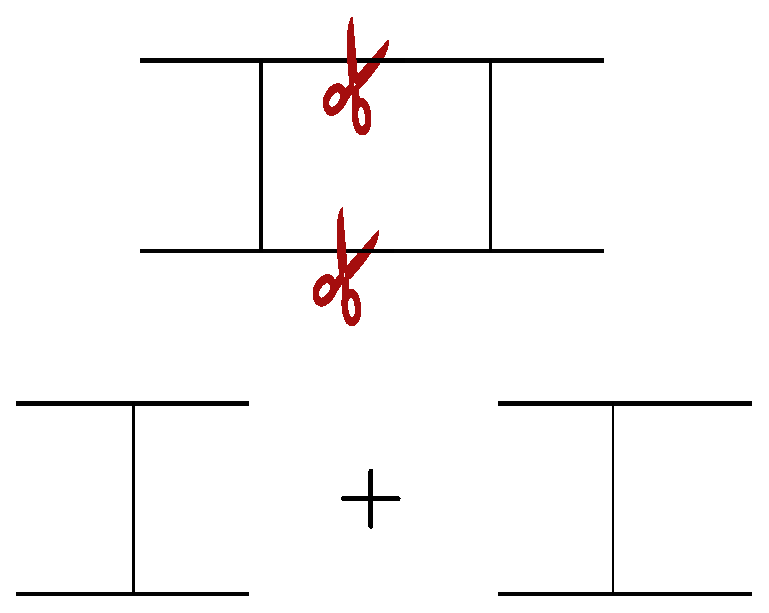
\includegraphics[scale=0.3]{Pictures/1partRedu_ladder.eps}
	\caption{Un diagrama escalera de dos partículas que se corta por los puntos indicados se convierte en dos diagramas de dos partículas, por lo tanto el diagrama inicial es reducible.}
	\label{fig:1partredu_ladder}
\end{figure}

Ahora, consideremos el caso en la Figura~\ref{fig:1parirred_mount}, donde tenemos un diagrama de una sola partícula que emite un fotón y lo reabsorbe. Al realizar un solo corte (pues el diagrama es de una partícula) por una linea interna, ya no obtenemos un diagrama de una partícula. Incluso podríamos pensar que el diagrama final es de dos partículas, pues tiene dos patas externas. Este diagrama, por consiguiente, \emph{es un diagrama irreducible de una partícula}.

\begin{figure}[ht]
	\centering
	
\includegraphics[scale=0.2]{1partIrred_mount.eps}
	\caption{Un diagrama de una partícula con un fotón que es emitido y reabsorbido. Al cortar por la línea indicada no se obtiene un diagrama de una partícula, por lo que este es un diagrama irreducible.}
	\label{fig:1parirred_mount}
\end{figure}

La idea general de los diagramas irreducibles es que a partir de ellos se pueden construir diagramas más complejos. Todo diagrama se puede construir a partir de diagramas irreducibles. Son una especie de equivalente de los números primos para el conjunto de los números naturales. Entonces, tengamos en cuenta lo siguiente: 

\begin{cabox}
	El concepto de grado superficial de divergencia será aplicado únicamente a diagramas irreducibles.
\end{cabox}

Con estos fundamentos claros, procedamos ahora a explorar de qué se trata el grado superficial de divergencia.

Típicamente, las expresiones correspondientes a un diagrama típico en QED serán de la forma
%
\begin{IEEEeqnarray}{rCl}
	\int \dd[4]{k_1} \dd[4]{k_2} \cdots \dd[4]{k_L} \frac{1}{\underbrace{(\slashed{k}_i - m)}_{\substack{\text{propagadores} \\ \text{de fermiones}}} \cdots \underbrace{k_j^2 \cdots k_n^2}_{\substack{\text{propagadores} \\ \text{de fotones}}}} 
\end{IEEEeqnarray}

El diagrama que consideramos tendrá tantas integrales en $k$ como loops hayan. Definiremos el grado superficial de divergencia como
%
\begin{equation}
\boxed{
	D = 4L - P_e - 2P_\gamma \,.
}
\end{equation}

Para comprender la el razonamiento detrás de esta expresión, consideremos lo siguiente: sabemos que por cada loop que hay en el diagrama habrá una integral $\dd[4]k_i$. Estamos interesados en la dimensión, en unidades de momento, del integrando. En unidades de momento, cada diferencial tiene dimensión $4$, i.e., cada loop aportará un $4$ a la dimensión del integrando. Ahora, los propagadores fermiónicos son de la forma
%
\begin{equation*}
	\frac{\ii}{\slashed{k} - m} \,,
\end{equation*}

\noindent de modo que, por cada propagador fermiónico la dimensión del integrando, en unidades de momento, disminuye en una unidad. Por su parte, los propagadores de fotones son de la forma
%
\begin{equation*}
	\frac{\ii}{k^2} \,,
\end{equation*}

\noindent haciendo que por cada propagador de fotones la dimensión del integrando, en unidades de momento, disminuya en dos unidades.

El grado superficial de divergencia, como podemos ver, es la dimensión del integrando en unidades de momento. Hablando de manera muy general, un diagrama diverge, a menos que hayan más potencias de momento en el denominador que en el numerador.

En general, podríamos esperar que el diagrama tenga una divergencia proporcional a $\Lambda ^D$, donde $\Lambda$ es un límite superior de los momentos, denominado \emph{corte} o \emph{cutoff}. En este escenario, podemos considerar los siguientes casos:

%
\begin{profor}
    \begin{equation*}
	\begin{IEEEeqnarraybox}[][c]{ll}
		\text{Si } D > 0 \qc & \text{la divergencia es proporcional a } \Lambda^D\,; \\
		%%%%
		\text{si } D = 0 \qc & \text{la divergencia es proporcional a } \log \Lambda \,; \\
		%%%%
		\text{si } D < 0 \qc & \text{las cantidades irań como } \Lambda^{-D} \text{ y son típicamente convergentes.}
	\end{IEEEeqnarraybox}
\end{equation*}
\end{profor}

Cabe anotar que esto no es una regla general. Existen diagramas que pueden contener divergencias no contempladas en este análisis, o diagramas convergentes cuyo grado superficial de divergencia puede ser igual a cero. No obstante, las condiciones dadas arriba se cumplen en muchos casos para los diagramas irreducibles.

Ahora, en QED el número de loops es dado por
%
\begin{equation}
	L = P_e + P_\gamma - \qty(V - 1) \,.
\end{equation}

Esto proviene de las reglas de Feynman, que exigen que por cada propagador debe haber una integral~\footnote{cf. David Griffiths. \emph{Introduction to Elementary Particles}. Second Edition. Wiley-VCH, 2008. Capítulos 6 y 7.}. No obstante, por cada vértice debe haber una delta de Dirac, que eliminará una de las integrales. Ahora, una de las deltas de Dirac expresará la conservación global del momento lineal, y esta delta no se integraba como las demás. A esta delta que no va a eliminar una integral se debe el $-1$ en el paréntesis. Finalmente, el número de loops es el número de integrales de cuatro dimensiones presentes en la expresión.

Para el número de vértices tenemos la expresión
%
\begin{equation}
	V = 2P_\gamma + N_\gamma \,,
\end{equation}

\noindent que se sigue de la estructura del vértice fundamental de QED, que siempre involucra un fotón. Si el fotón está como línea interna, debe estar asociado a dos vértices, mientras que si es una pata externa, estará asociado a uno solo. También es posible expresar el número de vértices como
%
\begin{equation}
	V = P_e + \frac{N_e}{2}\,,
\end{equation}

\noindent lo cual también responde a la estructura del vértice fundamental de QED.

Con estas expresiones podemos escribir el grado de divergencia como
%
\begin{IEEEeqnarray*}{rCl}
	D &=& 4L - P_e - 2\gamma \\
	%%%%
	&=& 4 \qty(P_e + P_\gamma - V + 1) - P_e - 2P_\gamma \\
	%%%%
	&=& 4 + 4P_\gamma + \cancel{4P_e} - 4 \qty(\cancel{P_e} + \frac{N_e}{2}) - P_e - 2P_\gamma \\
	%%%
	&=& 4 + 2P_\gamma - 2N_e - P_e \\
	%%%%
	&=& 4 + \cancel{2P_\gamma} - 2N_e - \qty(\cancel{2P_\gamma} + N_\gamma - frac{N_e}{2}) \\
	%%%%
	&=& 4 - 2N_e + \frac{N}{2} - N-\gamma \slj
	%%%%
	\IEEEeqnarraymulticol{3}{c}{\boxed{ D = 4 - \frac{3}{2}N_e - N_\gamma }\,. \IEEEyesnumber}
\end{IEEEeqnarray*}

Notemos que este resultado no depende de los propagadores, sino únicamente de las patas externas. \\


Para el caso de una teoría $\lambda \phi^n$, i.e. de la forma
%
\begin{equation}
	\lagdn = \frac{1}{2} (\partial_\mu \phi)(\partial^\mu \phi) - \frac{1}{2} m\phi^2 - \frac{\lambda}{n!} \phi^n \,,
\end{equation}

\noindent el número de loops será
%
\begin{equation}
	L = P - V + 1 \qc nV = N + 2P \,,
\end{equation}

\noindent puesto que sólo tenemos una partícula, y por lo tanto sólo tenemos propagadores y patas externas de una misma naturaleza. También se cumple que el grado de divergencia
%
\begin{equation}
	D = dL - 2P \,,
\end{equation}

\noindent donde $d$ es la dimensión de las integrales de momento, que en el caso de QED era 4, pero en este caso es arbitraria. Es posible mostrar que~\footnote{cf. Michael E. Peskin, Daniel V. Schroeder. \emph{An Introduction to Quantum Field Theory}. Addison-Wesley, 1995. Capítulo 10.}
%
\begin{equation}
	D = d + \qty[n \qty(\frac{d-2}{2}) - d]V - \frac{d-2}{2}N \,.
\end{equation} \\


Ahora, recordemos un poco las dimensiones que tienen algunas cantidades en unidades naturales. Al definir unidades naturales se tiene que la constante de Planck $h = 1$, es decir tiene dimensión cero en unidades naturales. Como $h$ tiene unidades de acción, esto hace que la acción tenga dimensión cero en unidades naturales, $[S] = 0$, y como
%
\begin{equation*}
	S = \int \dd[4]{x} \lagdn \,,
\end{equation*}

\noindent la dimensión del Lagrangiano es $-4$,
%
\begin{equation*}
	[\lagdn] = -4 \,,
\end{equation*}

Recordemos también cómo se define el momento lineal
%
\begin{equation*}
	\vb*{p} = m \vb*{v} \,.
\end{equation*}

Las velocidades son adimensionales en unidades naturales, en virtud de que $v = \dd x / \dd t$, y en unidades naturales la distancia y el tiempo tienen las mismas unidades, ya que $c = 1$. Esto implica que $ct = x$ y que el momento tenga unidades de masa.

Ahora, el momento angular
%
\begin{equation*}
	\vb*{L} = \vb*{x} \cross \vb*{p}
\end{equation*}

\noindent es adimensional, por lo que las $x$ deben tener unidades de $p^{-1}$. Volviendo a la acción, vemos entonces que el diferencial $\dd[4]x$ tiene magnitud $-4$ en unidades de momento, por lo que la densidad lagrangiana, en unidades de momento tiene magnitud
%
\begin{equation}
	[\lagdn] = 4 \qc \text{ en unidades de momento.}
\end{equation}

Consideremos la densidad lagrangiana como la diferencia entre una densidad de energía cinética y una densidad de potencial, $\lagdn = \mathcal{T} - \mathcal{V}$, y consideremos un potencial de la forma
%
\begin{equation}
	V = \sum_{n = 1}^{\infty} \frac{G_n}{n!} \phi^n \,,
\end{equation}

\noindent donde $G_n$ son constantes de acoplamiento.

Como $[\lagdn] = 4$ y el Lagrangiano contiene el término $-m^2 \phi^2$, cuya magnitud debe ser también 4, considerando que $[m] = 1$, tenemos que $[\phi] = 1$. Así pues, para el término en el potencial 
%
\begin{equation}
	\qty[\frac{G_4}{4!} \phi^4] = [G_4]4 = 4\,,
\end{equation}

\noindent de modo que el acoplamiento $G_4$ debe ser adimensional. Entonces, lo que tenemos para las unidades de los acoplamientos es que
%
\begin{equation}
	[G_n] = 4 - n \,.
\end{equation}

Vamos a clasificar los Lagrangianos según el siguiente criterio que enunciamos sin explicación, por el momento:
%
\begin{profor}
\begin{equation*}
	\begin{IEEEeqnarraybox}[][c]{ll}
		\text{si } [G_n] > 0 \qc & \text{decimos que la teoría es \emph{super-renormalizable;}} \\
		%%%%
		\text{si } [G_n] = 0 \qc & \text{decimos que la teoría es \emph{renormalizable;}} \\
		%%%%
		\text{si } [G_n] < 0 \qc & \text{decimos que la teoría es \emph{no-renormalizable.}}  
	\end{IEEEeqnarraybox}
\end{equation*}
\end{profor}

La idea, en general, será que las teorías que incluyen términos con potencias menores o iguales que $4$ tendrán buenas propiedades bajo normalización, mientras que aquellas que incluyan términos con potencias mayores que $4$ presentarán complicaciones para su normalización. 

En el caso de los fermiones, tenemos que en la ecuación de Dirac aparece el término $-m\overline{\psi} \psi$ , que debe tener dimensión 4, de modo que
%
\begin{IEEEeqnarray}{rCl}
	\left[-m \overline{\psi} \psi \right] &=& 4 \\
	%%%%
	1 + 2[\psi] &=& 4 \\
	%%%%
	\therefore [\psi] &=& \frac{3}{2} \,.
\end{IEEEeqnarray}


Por ejemplo, consideremos el Lagrangiano de Fermi
%
\begin{equation}
	\lagdn = G_F J_\mu J^\mu \,,
\end{equation}

\noindent donde
%
\begin{equation}
	J_\mu = \overline{\psi} \gamma^\mu \psi \quad \therefore \quad [J_\mu] = 3 \,,
\end{equation}

\noindent de modo que el operador $J_\mu J^\mu$ tiene dimensión 6, con lo cual
%
\begin{equation}
	[G_F] = -2\,,
\end{equation}

\noindent la teoría de Fermi es no-renormalizable.


Estas denominaciones para los Lagrangianos son mencionadas aquí sin más, a manera de definiciones. La justificación para ellas es complicada y la desarrollaremos a medida que veamos los ejemplos particulares en este capítulo.




%------------------------------------------------------
\section{Teoría de perturbación renormalizada}

Ahora, para obtener expresiones que resulten en amplitudes finitas, aún cuando tratemos con diagramas divergentes, el Lagrangiano ha de contener una masa desnuda $m_0$ y constante de acoplamiento desnudas $\lambda_0$ que sean consistentes con la teoría hasta un límite superior $\Lambda$ de los momentos. Este Lagrangiano que incorpora tales cantidades se denomina \emph{Lagrangiano desnudo}. Consideremos el Lagrangiano desnudo
%
\begin{equation}
	\lagdn = \frac{1}{2} \partial_\mu\phi \partial^\mu\phi - \frac{1}{2}m_0^2 \phi^2 - \frac{\lambda_0}{4!} \phi^4 \,.
\end{equation}

Para ciertos propósitos es deseable definir el campo $\phi$ como
%
\begin{equation}
	\phi = \sqrt{Z} \phi_r \,,    
\end{equation}

\noindent donde $Z$ es un parámetro denominado renormalización de la función de onda, y $\phi_r$ será el campo renormalizable. Con esto tenemos que el Lagrangiano es dado por
%
\begin{equation}
	\lagdn = \frac{1}{2} Z \qty(\partial_\mu\phi_r)\qty(\partial^\mu\phi_r)  - \frac{m_0^2}{2} Z \phi_r^2 - \frac{\lambda_0}{4!} Z^2 \phi_r^4\,.
\end{equation}

En la teoría renormalizada, buscaremos que el coeficiente acompañando el cuadrado de la derivada parcial sea $\sfrac{1}{2}$, de modo que es deseable redefinir $Z$ como $1$ más un pequeño incremento para dar cuenta de las discrepancias que puedan existir. Además, el término proporcional al cuadrado es el término de masa, por lo que esperaríamos que el coeficiente acompañando a $\phi^2$ sea el cuadrado de la masa física. Por ello redefiniremos el coeficiente en el Lagrangiano como el cuadrado de la masa física $m$ más un pequeño incremento. De la misma forma, el coeficiente del último término debería ser simplemente la constante de acoplamiento renormalizada, y por ello redefinimos el coeficiente también. Las redefiniciones que hemos hecho son
%
\begin{equation}
	Z = 1 + \delta_Z \qc m_0^2Z = m^2 + \delta_m \qc \lambda_0 Z^2 = \lambda + \delta_\lambda \,.
	\label{eq:redef_Lag_renorm}
\end{equation}

Con esto, podemos escribir el Lagrangiano en términos de las cantidades físicas y renormalizadas como
%
\begin{equation}
	\lagdn = \frac{1}{2} \qty(\partial_\mu\phi_r)\qty(\partial^\mu\phi_r) - \frac{1}{2} m^2 \phi_r^2 - \frac{\lambda}{4!} \phi_r^4 + \underbrace{\frac{1}{2} \delta_Z \qty(\partial_\mu\phi_r)\qty(\partial^\mu\phi_r) - \frac{1}{2} \delta_m \phi_r^2 - \frac{\delta_\lambda}{4!} \phi_r^4}_{\text{contratérminos}} \,.
\end{equation}

Tenemos entonces un Lagrangiano que depende de las cantitades físicas y renormalizadas, y que contiene los denominados contratérminos, que nos ayudarán a absorber los infinitos que surjan en las amplitudes como consecuencia de haber sustituído las cantidades desnudas en el Lagrangiano. Es tentador pensar que hemos agregado los contratérminos al Lagrangiano, pero de \eqref{eq:redef_Lag_renorm} vemos que simplemente las cantidades desnudas han sido divididas en dos componentes, una que es la cantidad física, y un incremento que expresa la discrepancia con estas últimas, y que va a contener los infinitos de la teoría.

Del nuevo Lagrangiano es posible leer las siguientes reglas de Feynman:

\begin{figure}[h!]
\begin{center}
	\begin{tabular}[H]{cl}
		\begin{minipage}[c]{0.5\textwidth}
			\centering
			
\includegraphics[scale=0.25]{RFeynmanRenorm1.eps}
		\end{minipage}
		& $= \dfrac{\ii}{p^2 - m^2 + \ii \epsilon}$ \\
		& \\
		\begin{minipage}[c]{0.5\textwidth}
			\centering
			
\includegraphics[scale=0.25]{RFeynmanRenorm2.eps}
		\end{minipage}
		& $= -\ii \lambda$ \\
		& \\
		\begin{minipage}[c]{0.5\textwidth}
			\centering
			
\includegraphics[scale=0.25]{RFeynmanRenorm3}
		\end{minipage}
		& $= \ii \qty(-\partial_\mu \partial^\mu \delta_Z - \delta_m) = \ii \qty(p^2 \delta_Z - \delta_m)$ \\
		& \\
		\begin{minipage}[c]{0.5\textwidth}
			\centering
			
\includegraphics[scale=0.25]{RFeynmanRenorm4}
		\end{minipage}
		& $= -\ii \delta_\lambda$
	\end{tabular}
\end{center}
\caption{Reglas de Feynman para una teoría $\lambda \phi^4$ en renormalización.}
\label{fig:rFeynman_contraterminos}
\end{figure}

El primer diagrama corresponde al propagador del campo escalar (que fue derivado en la sección \textcolor{red}{****seccion libro QFT****}. El segundo término proviene del término cuadrático en el campo. En general, las reglas de Feynman pueden leerse de un Lagrangiano mediante la siguiente prescripción:

\begin{cabox}
	Primero, las reglas de Feynman requieren que el Lagrangiano esté multiplicado por $\ii$. Habiendo hecho esto, los diagramas y el factor de vértice se obtienen según:
	
	\begin{itemize}
		\item Los campos que aparezcan en el término dan el grafo del diagrama de Feynman. Así, un término que incorpore, por ejemplo, $A^\mu \phi \phi$ representa un vértice en el que convergen un fotón (campo $A$) y dos campos escalares $\phi$.
		
		\item Si quitamos los campos del término, obtenemos la expresión para el factor de vértice. Por ejemplo, el término que consideramos $-\lambda/4! \phi^4$ implica que el factor de vértice sea $-\ii \lambda$.
	\end{itemize}
	
	Ahora, el factor $1/4!$ desaparece del factor de vértice debido a que hay 4 campos en el término. Cuando se integra la acción, el hecho de tener un número $n$ de campos implicará que aparecerá un factor $n!$, que se va a cancelar exactamente con el denominador.
\end{cabox}

Con esta prescripción es posible determinar los otros dos diagramas, que provienen de los contratérminos, hecho que es indicado con el símbolo $\otimes$ en el centro del diagrama. Para el primer diagrama de contratérminos tomamos los dos términos que incorporan dos campos en sus expresiones, i.e. $\frac{1}{2} \delta_Z \qty(\partial_\mu\phi_r)\qty(\partial^\mu\phi_r) - \frac{1}{2} \delta_m \phi_r^2$. Estos términos indican un campo entrando y uno saliendo. Para determinar el factor de vértice, no obstante, debemos realizar una modificación al primer término, integrando por partes:
%
\begin{IEEEeqnarray*}{rCl}
	\int \qty(\partial_\mu\phi_r)\qty(\partial^\mu\phi_r) \dd[4]{x} &=& \int \partial_\mu \qty(\phi \partial^\mu \phi) \dd[4]{x} - \int \phi \partial_\mu \partial^\mu \phi \dd[4]{x} \,.
\end{IEEEeqnarray*}

Ahora, usando el teorema de Gauss en cuatro dimensiones podemos escribir
%
\begin{IEEEeqnarray*}{rCl}
	\int \qty(\partial_\mu\phi_r)\qty(\partial^\mu\phi_r) \dd[4]{x} &=& \int_{\partial \Omega} \dd{S_\mu} \qty(\phi \partial^\mu \phi) - \int \phi \partial_\mu \partial^\mu \phi \dd[4]{x} \,,
\end{IEEEeqnarray*}

\noindent donde $\dd{S_\mu}$ es el elemento de volumen que apunta hacia afuera sobre la frontera $\partial \Omega$. En general, esta superficie se considera arbitrariamente grande, y se asume que $\partial^\mu \phi$ debe hacerse cero en esta región, para evitar que la energía del campo sea infinita \textcolor{red}{****revisar este argumento****}, por lo que se asume que la primera integral en el lado derecho se hace cero, obteniendo así
%
\begin{equation}
	\qty(\partial_\mu\phi_r)\qty(\partial^\mu\phi_r) \dd[4]{x} = - \int \phi \partial_\mu \partial^\mu \phi \dd[4]{x} \,,
\end{equation}

\noindent con lo cual los contratérminos en el Lagrangiano que inforporan dos campos son equivalentes a
%
\begin{equation}
	-\frac{1}{2} \delta_Z \phi_r \partial_\mu \partial^\mu \phi_r - \frac{1}{2} \delta_m \phi_r^2 \,,
\end{equation}

de donde obtenemos el tercer diagrama de Feynman y quedamos con el término de vértice $\ii \qty(-\delta_Z\partial_\mu \partial^\mu - \delta_m) = \ii \qty(p^2 \delta_Z - \delta_m)$, donde la igualdad se tiene porque $p = \ii\partial_\mu$, de acuerdo con las reglas de cuantización.

La última regla de Feynam se obtiene directamente del contratérmino proporcional a $\phi_r^4$.\\


Las definiciones que hemos empleado para la renormalización (Ec.~\eqref{eq:redef_Lag_renorm}) no son útiles a menos que establezcamos definiciones precisas de la masa y la constante de acoplamiento. Para ello, establecemos las siguientes \textbf{condiciones de renormalización}
 
\begin{center}
	\begin{tabular}[H]{cl}
		\begin{minipage}[c]{0.4\textwidth}
			\centering
			
\includegraphics[scale=0.5]{renorm_1linea.eps}
		\end{minipage}
		& \begin{minipage}[c]{0.6\textwidth}
			\begin{IEEEeqnarray*}{l}
				= \dfrac{1}{p^2 - m^2} + \substack{\text{ términos finitos en } \\ p^2 = m^2} \,; \hspace{2cm}
			\end{IEEEeqnarray*}
		\end{minipage} \\
		& \\
		\begin{minipage}[c]{0.4\textwidth}
			\centering
			
\includegraphics[scale=0.5]{renorm_4lineas.eps}
		\end{minipage}
		& \begin{minipage}[c]{0.6\textwidth}
			\begin{IEEEeqnarray}{l}
				= -\ii \lambda \qc s = 4m^2,\, t = u = 0 \hspace{2cm} \phantom{a} \label{eq:condRenorm_lambdaphi4}
			\end{IEEEeqnarray}
		\end{minipage}
	\end{tabular}
\end{center}

El primer diagrama indica la forma que imponemos a la función de Green de dos puntos, para la propagación de un cuerpo. La forma de la expresión indica que la amplitud invariante tendrá un polo en la masa física. El segundo diagrama indica la forma de la amplitud invariante para una dispersión dos-a-dos, con $s,\, t,\,u$ son variables de Mandelstam dadas por
%
\begin{equation}
	\begin{IEEEeqnarraybox}[][c]{rCl}
		s &=& \qty(p_1 + p_2)^2 \,, \slj
		%%%%
		t &=& \qty(p_1 - p_3)^2 = \qty(p_2 - p_4)^2\,, \slj
		%%%%
		u &=& \qty(p_1 - p_4)^2 = \qty(p_2 - p_3)^2\,. \\
	\end{IEEEeqnarraybox}
\end{equation}

Estas relaciones se obtienen de la conservación de momentum,
%
\begin{IEEEeqnarray*}{c}
	p_1 + p_2 = p_3 + p_4 \slj
	%%%%
	\therefore p_1 - p_3 = p_4 - p_2 \Rightarrow \qty(p_1 - p_3)^2 = \qty(p_2 - p_4)^2 \,. \IEEEyesnumber
\end{IEEEeqnarray*}

Lo que hemos hecho aquí para renormalizar es elegir un momentum en el cual se evalúa la amplitud del diagrama. En este valor específico de momentum, tenemos libertad para elegir cuánto vale la amplitud. 

Ahora podemos usar las nuevas reglas de Feynman para determinar cualquier amplitud en una teoría $\lambda \phi^4$. El procedimiento es el siguiente: Determinar la amplitud deseada como la suma de todos los diagramas posibles creados del propagador y vértices en la Fig.~\ref{fig:rFeynman_contraterminos}. Las integrales de loop en los diagramas, generalmente, serán divergentes, de modo que necesitamos introducir un regulador. El resultado de este cálculo será una función con tres parámetros desconocidos $\delta_Z,\, \delta_m$ y $\delta_\lambda$. Ajustar (o ``renormalizar'') estos tres parámetros según sea necesario para mantener las condiciones de renormalización \eqref{eq:condRenorm_lambdaphi4}. Después de este ajuste, la expresión para la amplitud debe ser finita e independiente del regulador.

Este procedimiento que emplea diagramas de Feynman con tontratérminos se denomina \emph{teoría de perturbación renormalizada}.


\textcolor{red}{Agregar discurso sobre los contratérminos siendo de un orden superior a los términos a tree-level}



%%%%%%%%%%
\subsection{Divergencias originadas de la dispersión dos-a-dos}

Vamos a calcular la amplitud de una dispersión dos-a-dos al nivel de un loop.

\begin{IEEEeqnarray*}{rCl}
	\ii \aminv \qty(p_1p_2 \rightarrow p_3p_4) &=& 
	\begin{gathered}
		
\includegraphics[scale=0.25]{renorm_2a2_1loop.eps}
	\end{gathered} \slj
	%%%%
	&=&
	\begin{gathered}
		
\includegraphics[scale=0.25]{renorm_X.eps}
	\end{gathered} + \left(\,
	\begin{gathered}
		
\includegraphics[scale=0.25]{renorm_xox.eps}
	\end{gathered} +
	\begin{gathered}
		
\includegraphics[scale=0.25]{renorm_oxx.eps}
	\end{gathered} +
	\begin{gathered}
		
\includegraphics[scale=0.25]{renorm_oxx_cruzado.eps}
	\end{gathered}
	\,\right) + \cdots \\
	&& - \underbrace{\ii \delta_\lambda}_{\text{contratérmino}} \,. \IEEEyesnumber 
\end{IEEEeqnarray*}

Debemos tener en cuenta que las divergencias no se presentan a nivel árbol (primer diagrama en la segunda línea), sino en términos con loops. Vamos a trabajar, entonces, el primer término a un loop. Para el análisis introduciremos los momentos dentro del loop como $k$ y $k-p$ que van en sentidos opuestos, de manera que $-k + k+p = p$, lo cual es consistente con la conservación de momentum, donde $p = p_1 + p_2$, así
%
\begin{IEEEeqnarray*}{rCl}
	\begin{gathered}
		
\includegraphics[scale=0.35]{renorm_loop1.eps}
	\end{gathered} 
	&=& \frac{\qty(-\ii \lambda)^2}{2}
	\int \frac{\dd[4]{k}}{(2 \pi)^4} 
	\frac{\ii}{k^2 - m^2 + \ii \epsilon}
	\frac{\ii}{(k + p)^2 - m^2 +\ii \epsilon} \\
	%%%%
	&\equiv& \qty(-\ii \lambda)^2 \ii V(p^2) = \qty(-\ii \lambda)^2 \ii V(s) \,, \IEEEyesnumber \label{eq:renorm_loop1}
\end{IEEEeqnarray*}

donde el $2$ que aparece en el denominador del factor de vértice en la primera linea es un factor de simetría que debe agregarse, pero cuya necesidad no demostraremos en este momento. Veamos otro diagrama \textcolor{red}{buscar lo que dice Peskin sobre factores de simetría y agregarlo}
%
\begin{equation}
	\begin{gathered}
		
\includegraphics[scale=0.35]{renorm_loop2.eps}
	\end{gathered} = 
	\begin{gathered}
		
\includegraphics[scale=0.35]{renorm_loop2_rot.eps}
	\end{gathered} = (-\ii \lambda)^2 \ii V\big( (p_1 - p_3)^2 \big)  = (-\ii \lambda)^2 \ii V(t) \,.
\end{equation}

Los dos diagramas que se muestran son equivalentes, y el segundo es muy similar al que aparece en la Ecuación~\eqref{eq:renorm_loop1}, excepto que $p_3$ y $p_2$ están invertidos respecto a éste, i.e., en este caso $p = p_1 - p_3 = p_4 - p_2$. Esto justifica la asignación de $V(p_1 - p_3)$ en lugar de $V(p)$.

Es posible mostrar que el diagrama cruzado tiene una amplitud dada por $(-\ii \lambda)^2  \ii V(u)$, y en general, la amplitud será de la forma
%
\begin{equation}
	\ii \aminv = -\ii \lambda + \qty(-\ii \lambda)^2 \qty[\ii V(s) + \ii V(t) + \ii V(u)] - \ii \delta_\lambda \,.
\label{eq:renorm_amplitud}
\end{equation}

De acuerdo con la condición de renormalización \eqref{eq:condRenorm_lambdaphi4}, esta amplitud debe ser igual a $-\ii \lambda$ cuando $s=4m^2,\, t=u=0$, lo cual implica que
%
\begin{IEEEeqnarray*}{C}
	\qty(-\ii \lambda)^2 \qty[\ii V(4m^2) + \ii V(0) + \ii V(0)] - \ii \delta_\lambda = 0 \slj
	%%%%
	\therefore \delta_\lambda = -\lambda^2 \qty[V\qty(4m^2) + 2V(0)] \,. \label{eq:delta_lambda} \IEEEyesnumber
\end{IEEEeqnarray*}

En este punto vemos la importancia de la elección de los valores de momentum en que definimos las condidicones de renormalización. nótese que de las cantidades $V(p)$ aparecerán infinitos debido a que representan loops. Estos infinitos serán contrarrestados por el contratérmino $\delta_\lambda$. Este contratérmino cancelará los infinitos para esta elección de momentum. Ahora, cuando decido variar $s,\, t,\, u$ a otro valor, los infinitos siguen siendo contrarrestados. Esto es, al exigir que, en un punto del espacio de momentos, la amplitud sea finita, estoy garantizando que cualquier valor arbitrario de los momentos también la amplitud sea finita. Es importante entender el procedimiento que hemos realizado para conseguir la eliminación de los infinitos, de modo que resumimos este proceso a continuación

\begin{cabox}
	Las cantidades a un loop son las que aportan infinitos, i.e., los $V$'s. Para eliminar estas divergencias, fijamos el valor de la amplitud invariante del diagrama para un valor específico de los momentos. Se presume que la constante de acoplamiento puede ser medida para este valor preciso de momentos, de modo que, bajo estas condiciones, imponemos que la amplitud invariante sea igual a la masa multiplicada por la constante de acoplamiento, haciendo que el término que involucra a los $V$'s sea cero.	Al evaluar la amplitud para otros valores de momentos, el término con los $V$'s ya no es cero, no obstante, el término ya no presenta infinitos, y dará la evolución correcta y el comportamiento correcto de la amplitud $\aminv$ con los momentos para valores arbitrarios de $s,\, t,\, u$.
\end{cabox}

A continuación podremos manipular los $V$'s haciendo uso de los parámetros de Feynman (Feynman parameters)




%-----------------------------------------------------
\subsection{Parámetros de Feynman y rotación de Wick}

Si tenemos una expresión de la forma $\sfrac{1}{AB}$, esto puede escribirse como
%
\begin{equation}
	\frac{1}{AB} = \int_0^1 \dd{x} \frac{1}{\qty[xA + (1-x)B]^2} \,.
\end{equation}

\begin{proof}
	Sea
	%
	\begin{IEEEeqnarray*}{rll}
		U =& \, xA + (1-x)B \qquad \qquad & \\
		\Rightarrow \dd{U} = & \, (A-B)\dd{x} & \therefore \dd{x} = \frac{\dd{u}}{A-B} \IEEEyesnumber
	\end{IEEEeqnarray*}

	Reemplazando en la integral tenemos
	%
	\begin{IEEEeqnarray*}{rCl}
		\frac{1}{AB} &=& \int \frac{\dd{U}}{A-B} \frac{1}{U^2} \\
		%%%%
		&=& \frac{1}{A-B} \int U^{-2} \dd{U} \\
		%%%%
		&=& \eval{\frac{1}{A-B} \frac{U^{-2+1}}{-2+1} }_{x= 0}^{x=1} \\
		%%%%
		&=& \frac{(-1)}{A-B} \qty[\frac{1}{A} - \frac{1}{B}] \\
		%%%%
		&=& \frac{(-1)}{A - B} \frac{B-A}{AB} \\
		&=& \frac{1}{AB} \,.
	\end{IEEEeqnarray*}
\end{proof}

\hfill $\square \qquad\qquad$

Adicionalmente, es fácil probar que
%
\begin{equation}
	\boxed{\frac{1}{AB} = \int_0^1 \dd{x} \frac{1}{\qty[xA + (1-x)B]^2} = \int \frac{\dd{x} \dd{y} \delta(x + y -1)}{\qty[xA + yB]^2}} \,.
\end{equation}

La idea central de los parámetros de Feynman es convertir un producto en el denominador, a una suma en el denominador. Este resultado se puede generalizar para un número arbitrario de factores en el denominador
%
\begin{equation}
	\boxed{
	\frac{1}{A_1 A_2 \cdots A_n} = \int \dd{x_1} \dd{x_2} \cdots \dd{x_n} \delta\qty(\sum_i x_i - 1) \frac{(n-1)!}{\qty[x_1A_1 + x_2A_2 + \cdots + x_nA_n]}
	} \,.
\end{equation}

Apliquemos entonces, la técnica de los parámetros de Feynman a la expresión que teníamos para la amplitud invariante:
%
\begin{IEEEeqnarray*}{rCl}
	(-\ii \lambda)^2 \ii V(p^2) &=& - \frac{(-\ii \lambda)^2}{2} \int \frac{\dd[4]{k}}{(2 \cpi)^4} \frac{1}{k^2 - m^2} \frac{1}{(k+ p)^2 - m^2} \\
	%%%%
	&=& - \frac{(-\ii \lambda)^2}{2} \int_0^1 \frac{1}{\qty[x (k^2 - m^2) + (1 - x) \big( (k + p)^2 - m^2 \big)]^2} \,. \IEEEyesnumber \label{eq:calculo_FeynmanPar_1}
\end{IEEEeqnarray*}

Concentrémonos en el denominador, que llamaremos $D$, y manipulemos un poco la expresión:
%
\begin{IEEEeqnarray*}{rCl}
	D &=& x \qty(k^2 - m^2) + (1 - x) \qty(k^2 + 2k \vdot p + p^2 - m^2) \\
	%%%%
	&=& k^2\qty(x + 1 -x) + 2k\vdot p \qty(1-x) + (1-x)p^2 + m^2 \qty[-x -(1-x)] \\
	%%%%
	&=& k^2 + 2k\vdot p (1- x) + (1-x)p^2 - m^2 \,. \IEEEyesnumber
\end{IEEEeqnarray*}

A fin de hacer coincidir este resultado con la parametrización que, usualmente, aparece en la literatura, realizamos el siguiente cambio de variables
%
\begin{equation}
	1 - x = \tilde{x} \quad\Rightarrow\quad -\dd{x} = \dd{\tilde{x}} \,,
\end{equation}

\noindent de modo que
%
\begin{equation}
	D = k^2 + 2k\vdot p \tilde{x} + \tilde{x}p^2 - m^2 \,,
\end{equation}

\noindent y reemplazando en \eqref{eq:calculo_FeynmanPar_1},
%
\begin{IEEEeqnarray*}{rCl}
	\ii V(p^2) &=& -\frac{1}{2} \int \frac{\dd^4{k}}{(2\pi)^4} \int_1^0 (-\dd{\tilde{x}}) \frac{1}{D^2} \\
	%%%%
	&=& - \frac{1}{2} \int \frac{\dd^4 k}{(2\pi)^4} \int_0^1 \frac{\dd{x}}{\qty[k^2 + 2k\vdot px + xp^2 - m^2]^2} \,. \IEEEyesnumber \label{eq:calculo_FeynmanPar_2}
\end{IEEEeqnarray*}

Ahora, continuamos con la manipulación del denominador:
5
\begin{IEEEeqnarray*}{rCl}
	D &=& k^2 + 2k\vdot px \textcolor{orange}{\> + \> x^2p^2 - x^2p^2} + xp^2 - m^2 \\
	%%%%
	&=& \qty(k + xp^2)^2 + p^2x\qty(1 - x) - m^2 \\
	%%%%
	&=& \ell^2 + p^2x(1 - x) - m \,,
\end{IEEEeqnarray*}

\noindent donde $\ell$ es un cuadrivector, por lo que podemos definir
%
\begin{equation}
	\ell^2 = \ell_0^2 - \abs{\vb*{\ell}}^2 \,,
\end{equation}

\noindent con $\vb*{\ell}$ (en negrilla) es la componente espacial.
%
\begin{IEEEeqnarray}{rCl}
	\Rightarrow D &=& \ell_0^2 - \abs{\vb*{\ell}} - m^2 + x(1 - x)p^2 + \ii\epsilon \,,
\end{IEEEeqnarray}

y las raíces en $\ell_0$ de $D$ serán
%
\begin{equation}
	\ell_0 = \pm \sqrt{\abs{\vb*{\ell}} + m^2 - x(1-x)p^2 - \ii\epsilon} \,.
\end{equation}

Es importante recordar que, debido a las condiciones de renormalización que hemos impuesto, debemos evaluar esta expresión en $p^2 = 4m^2$, y por lo tanto es necesario mostrar que el radicando es una cantidad positiva para este valor. Tomamos la cantidad $\Delta = m^2 - x(1 - x)p^2$, puesto que, por definición, los otros dos términos del radicando ya son positivos. Tenemos:
%
\begin{IEEEeqnarray*}{rCl}
	\Delta = m^2 - x(1 - x)p^2 &=& m^2 x(1 - x)4m^2 \\
	%%%%
	&=& m^2\qty[1 - 4x + 4x^2] \\
	%%%%
	&=& m^2 \qty[1 - 2x]^2 \geq 0 \,.
\end{IEEEeqnarray*}

Con esto tenemos que
%
\begin{IEEEeqnarray*}{rCl}
	\ell_0 &=& \pm \sqrt{\abs{\vb*{\ell}}^2 + \Delta - \ii\epsilon} \\
	%%%%
	&=& \pm \sqrt{\qty(\abs{\vb*{\ell}}^2 + \Delta) \qty(1 - \frac{\epsilon}{\abs{\vb{\ell}}^2 + \Delta})} \\ 
	%%%%
	&=& \pm \sqrt{\abs{\vb*{\ell}}^2 + \Delta} \qty(1 - \frac{\ii}{2} \frac{\epsilon}{\abs{\vb{\ell}}^2 + \Delta}) \\
	%%%%
	&=& \pm \sqrt{\abs{\vb*{\ell} + \Delta}^2}\qty(1 - \ii \epsilon') \,, \quad \epsilon' \geq 0 \,. \IEEEyesnumber
\end{IEEEeqnarray*}

Tenemos entonces, que las dos raíces de $D$ son
%
\begin{equation}
	\ell_0 = \left\{
	\begin{IEEEeqnarraybox}[][c]{l}
		\IEEEstrut
		+ \sqrt{\abs{\vb*{\ell} + \Delta}^2} - \ii\epsilon \,, \slj
		%%%%
		- \sqrt{\abs{\vb*{\ell} + \Delta}^2} + \ii \epsilon \,.
		\IEEEstrut
	\end{IEEEeqnarraybox}
	\right.
\end{equation}

Podemos representar estas soluciones en el plano complejo, como se muestra en la Fig.~\ref{fig:renorm_complejo}, de modo que podemos trazar un contorno como el que se muestra con la linea azul, que no encierra ninguno de los polos. De esta forma, cuando extendemos el contorno hasta el infinito, podemos emplear el teorema del residuo para calcular la integral. 

\begin{figure}[ht]
	\centering
	
\includegraphics[scale=0.3]{renorm_complejo.eps}
	\caption{Representación de las soluciones $\ell_0$ en el plano complejo (puntos rojos), que son polos de la amplitud invariante, y los contornos empleados para la integración, que no encierran ningún polo.}
	\label{fig:renorm_complejo}
\end{figure}

La integral sobre el contorno se recorrerá de cero a infinito sobre el eje real, regresando por el arco $C_1$, luego hacia cero sobre el eje complejo. Como el contorno no encierra a ninguno de los polos, por teorema del residuo, la integral cerrada será igual a cero. Tenemos entonces,
%
\begin{IEEEeqnarray*}{rCl}
	0 &=& \int_0^\infty \dd{k_0} + \int_{C_1} \dd{k_0} f(k_0) + \int_{\ii\infty}^0 \dd{k_0} f(k_0)
\end{IEEEeqnarray*}

\noindent donde $k_0$ es un número complejo, $f$ es alguna función.

Para la trayectoria sobre el tercer cuadrante tenemos
%
\begin{IEEEeqnarray*}{rCl}
	0 &=& \int_0^{-\ii\infty} \dd{k_0} + \int_{C_2} \dd{k_0} f(k_0) + \int_{-\infty}^0 \dd{k_0} f(k_0) \,.
\end{IEEEeqnarray*}

Las funciones $f(k_0)$, generalmente, son de tal forma que las integrales sobre los arcos se hacern cero~\footnote{Asumimos esto aquí sin demostración. Para una demostración de este hecho ver \textcolor{red}{ref********}}, de modo que, sumando las integrales en los dos cuadrantes, tenemos
%
\begin{IEEEeqnarray}{rCl}
	\int_{-\infty}^{+\infty} \dd{k_0} f(k_0) + \int_{+\ii\infty}^{-\ii\infty} \dd{k_0} f(k_0) &=& 0 \,.
\end{IEEEeqnarray}

Ahora, como $k_0 = k_0^{\text{Re}} + \ii k_0^{\text{Im}}$, para el eje vertical $k_0^\text{Re} = 0 \Rightarrow k_0 = \ii k_0^\text{Im}$, de modo que
%
\begin{equation}
	\begin{IEEEeqnarraybox}[][c]{rClcl}
		k_{0\text{min}} &=& + \ii \infty = \ii k_{0\text{min}}^\text{Im} &\quad \Rightarrow \quad& k_{0\text{min}}^\text{Im} = +\infty \,, \slj
		%%%%
		k_{0\text{max}} &=& - \ii \infty = \ii k_{0\text{max}}^\text{Im} &\quad \Rightarrow \quad& k_{0\text{max}}^\text{Im} = -\infty \,.
	\end{IEEEeqnarraybox}
\end{equation}

Haciendo el cambio de variable $k_0 \longrightarrow k_0^\text{Im}$ podemos escribir
%
\begin{equation}
	\dd{k_0} = \dd{(\ii k_0^\text{Im})} = \ii \dd{k_0^\text{Im}} \,,
\end{equation}

\noindent y reemplazando en la integral,
%
\begin{equation}
	\int_{-\infty}^{+\infty} f(k_0) \dd{k_0} = - \int_{+\infty}^{-\infty} \dd{(\ii k_0^\text{Im})} f(\ii k_0^\text{Im}) = + \ii \int_{-\infty}^{+\infty} \dd{k_0^\text{Im}} f(\ii k_0^\text{Im}) \,.
\end{equation}

Definiendo $k_0^\text{Im} \equiv k_0^\text{E}$ (E por euclidiano) tenemos, finalmente
%
\begin{equation}
	\boxed{\int_{-\infty}^{+\infty} f(k_0) \dd{k_0}  = \int_{-\infty}^{+\infty} \dd{k_0^\text{E}} f(\ii k_0^\text{E})} \,,
	\label{eq:rotWick}
\end{equation}

\noindent resultado que se conoce como \textbf{Rotación de Wick}, que nos permite convertir cantidades del espacio de Minkowski al espacio euclidiano.\\


Volviendo a nuestro cálculo de la amplitud invariante, teníamos que
%
\begin{equation}
	\ii V(p^2) = -\frac{1}{2} \int \frac{\dd[4]{\ell}}{(2 \cpi)^4} \int_0^1 \dd{x} \frac{1}{\qty[\ell_0^2 - \abs{\vb*{\ell}}^2 - m^2 + x(1 - x)p^2 + \ii\epsilon]^2} \,,
\label{eq:iV_despuesDeRotWick}
\end{equation}

\noindent y nos enfocaremos en la integral sobre $\dd{\ell_0}$. Tendremos entonces que, una de las integrales de $\dd[4]\ell$ será de la forma
%
\begin{equation}
	\int_{-\infty}^{+\infty} \dd{\ell_0} f(\ell_0) = \ii \int_{-\infty}^{+\infty} \dd{\ell_0^\text{E}} f(\ii \ell_0) \,,
\end{equation}

\noindent donde $f(\ell_0)$ es el integrando en la Ecuación~\eqref{eq:iV_despuesDeRotWick}, y hemos aplicado la rotación de Wick. Entonces,
%
\begin{equation}
	\ii V(p^2) = -\frac{1}{2} \int \frac{\dd[3]{\ell}}{(2\cpi)^4} \ii \int_{-\infty}^{+\infty} \dd{\ell_0^\text{E}} \int_0^1 \dd{x} \frac{1}{\qty[-(\ell_0^\text{E})^2 - \abs{\vb*{\ell}}^2 - m^2 + x(1 - x)p^2 + \ii\epsilon]^2} \,.
\end{equation}

Nótese que mediante la rotación de Wick hemos logrado que, en el denominador, el cuadrado de la componente $\ell_0$ y el cuadrado de las componentes espaciales $\vb*{\ell}$ ya no se resten, sino que aparezcan como una suma. Esta es la importancia de este paso. Siguiendo con el cálculo,
%
\begin{equation}
	\ii V(p^2) = -\frac{\ii}{2} \int_0^1 \dd{x} \int \frac{\dd[4]{\ell_\text{E}}}{(2\cpi)^4} \frac{1}{\qty[\ell_\text{E}^2 + \Delta - \ii\epsilon]} \,,
\label{eq:iV(p)_antesDeRegDim}
\end{equation}

\noindent donde $\ell_\text{E}^2 = \qty(\ell_0^\text{E})^2 + \abs{\vb*{\ell}}^2$ y $\Delta = m^2 - x(1 - x)p^2$. Esta es una integral divergente. Para manipularla, introduciremos la técnica de la \emph{regularización dimensional}.




%------------------------------------------------------
\subsection{Regularización dimensional}

El proceso consiste en promover una integral en cuatro dimensiones a una integral en $d$ dimensiones. Posteriormente tomaremos el límite inferior cuando $d \rightarrow 4$. Las integrales, usualmente, convergen para $d<4$. Esta es la razón por la cual es conveniente trabajar con una dimensión menor que 4 para resolver la integral.

Tomemos como ejemplo la siguiente integral\footnote{En el denominador tenemos la expresión $\qty(\ell_E^2 + \Delta)^2$, donde ya no aparece el término $\ii\epsilon$ de la prescripción de Feynman. La razón para esto es que ahora tenemos únicamente valores reales. $\ell_E^2$ es un número positivo, así como $\Delta$, de modo que ya no hay posibilidades de que tengamos un polo para algún valor de $\ell_E$, y por lo tanto, podemos tomar $\epsilon=0$.}:
%
\begin{IEEEeqnarray*}{rCl}
	\int \frac{\dd[4]{\ell_E}}{(2\cpi)^4} \frac{1}{\qty(\ell_E^2 + \Delta)^2} &\longrightarrow& \int \frac{\dd[d]\ell_E}{(2\cpi)^d} \frac{1}{\qty(\ell_E^2 + \Delta)^2} \,. \IEEEyesnumber
\end{IEEEeqnarray*}

Esta integral puede escribirse en coordenadas esféricas (en $d$ dimensiones) de la siguiente forma:
%
\begin{IEEEeqnarray*}{rCl}
	\int \frac{\dd[d]\ell_E}{(2\cpi)^d} \frac{1}{\qty(\ell_E^2 + \Delta)^2} &=& \int \dd{\Omega_d} \int_0^\infty \frac{\dd{\ell_E}}{\qty(\ell_E^2 + \Delta)^2} \,, \label{eq:regularizacion_intEsf} \IEEEyesnumber
\end{IEEEeqnarray*}

\noindent donde $\Omega$ es la variable del ángulo sólido. Emplearemos el siguiente "truco": como
%
\begin{equation*}
	\sqrt{\cpi} = \int_{-\infty}^{\infty} \ee^{- x^2} \dd{x} \qquad \text{es la integral de una gaussiana,}
\end{equation*}

\noindent entonces,
%
\begin{IEEEeqnarray*}{rCl}
	\qty(\sqrt{\cpi})^d &=& \qty(\int_{-\infty}^{\infty} \dd{x_1} \ee^{- x_1^2})^d \\
	%%%%
	&=& \qty(\int_{-\infty}^{\infty} \dd{x_1} \ee^{- x_1^2}) \qty(\int_{-\infty}^{\infty} \dd{x_2} \ee^{- x_2^2}) \cdots \qty(\int_{-\infty}^{\infty} \dd{x_d} \ee^{- x_d^2}) \\
	%%%%
	&=&  \int_{-\infty}^{\infty} \dd{x_1} \dd{x_2} \cdots \dd{x_d} \ee^{-\sum_{j = 1}^d x_j^2} \\
	%%%%
	&=& \int_{-\infty}^{\infty} \dd[d]{x} \ee^{-(\vb*{x})^2} \,, \label{eq:sqrtpi2} \IEEEyesnumber
\end{IEEEeqnarray*}

\noindent donde
%
\begin{equation}
	\qty(\vb*{x})^2 = \sum_{j=1}^d x_j^2 \equiv x^2 \qquad \therefore\> x = \sqrt{\sum_{j=1}^d x_j^2} \,.
\end{equation}

Ahora, en coordenadas esféricas ($d$-dimensionales) tenemos que~\footnote{Por ejemplo, para el caso de tres dimensiones tenemos $\dd[3]{x} = r^2 \dd{\Omega}$, con $r = \sqrt{x^2 + y^2 + z^2}$.}
%
\begin{equation}
	\dd[d]{x} = x^{d - 1} \dd{\Omega_d} \,.
\end{equation}

Con esto en \eqref{eq:sqrtpi2} tenemos
%
\begin{equation}
	\qty(\sqrt{\cpi})^d = \int \dd{\Omega_d} \underbrace{\int \dd{x} x^{d-1} \ee^{-x^2}}_{\frac{1}{2} \Gamma(\frac{d}{2})} \,,
\end{equation}

\noindent donde, la integral en $x$ es una expresión conocida en la literatura y es dada por la función gamma que hemos indicado. Como este factor es conocido, al igual que $\sqrt{\cpi}$, es posible determinar la integral en el ángulo sólido. Entonces
%
\begin{IEEEeqnarray}{rCl}
	\int \dd{\Omega_d} = \frac{2 \qty(\sqrt{\cpi})^d}{\Gamma(\frac{d}{2})} = \frac{2 \cpi^{d/2}}{\Gamma(\frac{d}{2})} \,.
\end{IEEEeqnarray}

En la Tabla~\ref{tb:intAnguloSolido} se dan los valores que arroja esta expresión para $d$ entre 1 y 4.

\begin{table}[h!]
	\centering
	\caption{Valores de la integral sobre el ángulo sólido en diferentes dimensiones $d$.}
	\begin{tabular}{C{1cm} *2{C{2cm}}}
		\hline\hline
		$d$ & $\Gamma(\frac{d}{2})$ & $\int \dd{\Omega_d}$ \\ \hline
		%%%%%%%%%%
		$1$ & $\sqrt{\cpi}$ & $2$ \\
		%%%%
		$2$ & $1$ & $2\cpi$ \\
		%%%%
		$3$ & $\sqrt{\cpi}/2$ & $4\cpi$ \\
		%%%%
		$4$ & $1$ & $2\cpi^2$ \\
		\hline\hline
	\end{tabular}
	\label{tb:intAnguloSolido}
\end{table}

Volviendo a \eqref{eq:regularizacion_intEsf}, teníamos
%
\begin{equation}
	\int \frac{\dd[d]\ell_E}{(2\cpi)^d} \frac{1}{\qty(\ell_E^2 + \Delta)^2} = \underbrace{\int \dd{\Omega_d}}_{\substack{\text{Integral}\\\text{angular}}} \underbrace{\int_0^\infty \frac{\dd{\ell_E}}{\qty(\ell_E^2 + \Delta)^2}}_{\substack{\text{Integral}\\\text{radial}}} \,,
	\tag{\ref{eq:regularizacion_intEsf}}
\end{equation}

\noindent donde ya hemos encontrado el valor de la integral angular. Para la integral radial, haciendo el cambio de variable
%
\begin{IEEEeqnarray*}{rCl}
	x = \ell^2 \quad &\Rightarrow& \dd{x} = 2\ell \dd{\ell} \slj
	&\therefore& \dd{\ell} = \frac{\dd{x}}{2\sqrt{x}} \,,
\end{IEEEeqnarray*}

\noindent tenemos
%
\begin{IEEEeqnarray*}{rCl}
	\int_0^\infty \frac{\dd{\ell_E}}{\qty(\ell_E^2 + \Delta)^2} &=& \int_0^\infty \frac{\dd{x}}{2\sqrt{x}} \frac{x^{(d - 1)/2}}{\qty(x + \Delta)^2} \\
	%%%%
	&=& \frac{1}{2} \int_0^\infty \dd{x} \frac{x^{\frac{d}{2} - 1}}{\qty(x + \Delta)^2} \,.
\end{IEEEeqnarray*}

Haciendo un segundo cambio de variable,
%
\begin{IEEEeqnarray*}{Cll}
	& z = \frac{\Delta}{x + \Delta} \,; \quad & \begin{IEEEeqnarraybox}[][c]{l}
		z_\text{min} = z(0) = 1 \,, \\
		%
		z_\text{max} = z(\infty) = 0\,.
	\end{IEEEeqnarraybox} \slj
	%%%%
	\Rightarrow& x = \frac{\Delta(1 - z)}{z}& \slj
	%%%%
	\therefore& \dd{x} = -\frac{\Delta}{z^2} \dd{z} \,,&
\end{IEEEeqnarray*}

\noindent de modo que
%
\begin{IEEEeqnarray*}{rCl}
	\int_0^\infty \frac{\dd{\ell_E}}{\qty(\ell_E^2 + \Delta)^2} &=& \frac{1}{2}\int_1^0 \qty[-\frac{\Delta}{\cancel{z^2}} \dd{z}] \frac{\Delta^{\frac{d}{2} - 1} (1-z)^{\frac{d}{2} - 1}}{z^{\frac{d}{2} - 1}} \frac{\cancel{z^2}}{\Delta^2} \\
	%%%%
	&=& \frac{1}{2}\int_0^1 \Delta^{\frac{d}{2} - 2} \qty(1 - z)^{\frac{d}{2} - 1} z^{1 - \frac{d}{2}} \dd{z} \,. \label{eq:rglzDim_1} \IEEEyesnumber
\end{IEEEeqnarray*}

Ahora, tenemos la siguiente identidad
%
\begin{equation}
	\int_0^1 z^{\alpha - 1} \qty(1 - z)^{\beta - 1} = \frac{\Gamma(\alpha) \Gamma(\beta)}{\Gamma(\alpha + \beta)} \,.
\end{equation}

Comparando con \eqref{eq:rglzDim_1} vemos que
%
\begin{IEEEeqnarray*}{c}
	\beta = \frac{d}{2} \,, \slj
	%%%%
	\alpha - 1 = 1 - \frac{d}{2} \quad\Rightarrow\quad \alpha = 2 - \frac{d}{2} \,,
\end{IEEEeqnarray*}

\noindent así,
%
\begin{IEEEeqnarray*}{rCl}
	\int_0^\infty \frac{\dd{\ell_E}}{\qty(\ell_E^2 + \Delta)^2} &=& \qty(\frac{1}{2}) \qty(\frac{1}{\Delta})^{2 - \frac{d}{2}} \frac{\Gamma(2 - \frac{d}{2}) \Gamma(\frac{d}{2})}{\Gamma(2)}\,, \IEEEyesnumber
\end{IEEEeqnarray*}

\noindent es la expresión final para la integral radial. Entonces, con esto en \eqref{eq:regularizacion_intEsf} tenemos que
%
\begin{IEEEeqnarray*}{rCl}
	\int \frac{\dd[d]\ell_E}{(2\cpi)^d} \frac{1}{\qty(\ell_E^2 + \Delta)^2} &=& \frac{\bcancel{2}\cpi^{\frac{d}{2}}}{\cancel{\Gamma(\frac{d}{2})}} \frac{1}{\bcancel{2}} \qty(\frac{1}{\Delta})^{2 - \frac{d}{2}} \frac{\Gamma(2 - \frac{d}{2}) \cancel{\Gamma(\frac{d}{2})}}{\Gamma(2)} \frac{1}{(2\cpi)^d} \lj
	%%%%
	\IEEEeqnarraymulticol{3}{c}{ \boxed{
	\int \frac{\dd[d]\ell_E}{(2\cpi)^d} \frac{1}{\qty(\ell_E^2 + \Delta)^2} = \frac{1}{\qty(4\cpi)^{\frac{d}{2}}} \Gamma\qty(2 - \frac{d}{2}) \qty(\frac{1}{\Delta})^{2 - \frac{d}{2}}
	} \,. \label{eq:regDim_integralCompleta} \IEEEyesnumber} 
\end{IEEEeqnarray*}

Ahora, vamos a emplear una expresión asintótica para $\Gamma$. Las expresiones asintótica son similares a las series de Taylor, pero en lugar de estar evaluadas en torno a cero, pueden tener términos divergentes. La expresión asintótica que nos interesa en este caso es
%
\begin{equation}
	\Gamma\qty(2 - \frac{d}{2}) = \Gamma \qty(\frac{4-d}{2}) = \Gamma\qty(\frac{\epsilon}{2}) = \frac{2}{\epsilon} - \gamma + \mathscr{O}(\epsilon) \,,
\end{equation}

\noindent donde 
%
\begin{equation}
	\epsilon = 4 - d > 0; \qquad \gamma = 0.5772 \,.
\end{equation}

En general, estas expresiones convergen para $0 < d < 4$, y divergen para $d =4$. Estas son las divergencias ultravioletas que debemos eliminar de la teoría. Introduciendo la expansión asintótica en \eqref{eq:regDim_integralCompleta} tenemos
%
\begin{equation}
	\int \frac{\dd[d]\ell_E}{(2\cpi)^d} \frac{1}{\qty(\ell_E^2 + \Delta)^2} = \frac{1}{(4\cpi)^{d/2}} \qty[\frac{2}{\epsilon} - \gamma + \mathscr{O}(\epsilon)] \Delta^{-\epsilon/2} \,,
\end{equation}

\noindent con  $\frac{\epsilon}{2} = 2 - \frac{d}{2} = \frac{4-d}{2} = \frac{\epsilon}{2}$. Ahora, 
%
\begin{IEEEeqnarray*}{c}
	(4\cpi)^{d/2} = \frac{(4\cpi)^{2 - \frac{d}{2}}}{(4\cpi)^2} = \frac{(4\cpi)^{\epsilon/2}}{(4\cpi)^2} \slj
	%%%%
	\Rightarrow \frac{1}{(4\cpi)^{d/2}} \Delta^{-\epsilon/2} = \frac{1}{(4\cpi)^2} \qty[\frac{4\cpi}{\Delta}]^{\epsilon/2} = \frac{1}{(4\cpi)^2} \ee^{\frac{\epsilon}{2} \ln\qty(\frac{4\cpi}{\Delta})} \,.
\end{IEEEeqnarray*}

Teniendo en cuenta que $\epsilon$ es pequeño, la exponencial puede expandirse en series de Taylor~\footnote{$\ee^{x} \approx 1 + x$, \quad si $x \ll 1$.}, y entonces tenemos que 
%
\begin{IEEEeqnarray*}{rCl}
	\int \frac{\dd[d]\ell_E}{(2\cpi)^d} \frac{1}{\qty(\ell_E^2 + \Delta)^2} &\approx& \frac{1}{(4\cpi)^{2}} \qty[\frac{2}{\epsilon} - \gamma + \mathscr{O}(\epsilon)] \qty[1 + \frac{\epsilon}{2}\ln(\frac{4\cpi}{\Delta})] \\
	%%%%
	&=& \frac{1}{(4\cpi)^2} \qty[\frac{2}{\epsilon} - \gamma + \ln(\frac{4\cpi}{\Delta}) + \mathscr{O}(\epsilon)] \\
	%%%%
	&=& \frac{1}{(4\cpi)^2} \qty[\frac{2}{\epsilon} - \gamma + \ln(4\cpi) - \ln(\Delta) + \mathscr{O}(\epsilon)] \,. \label{eq:potencial_delta_lambda} \IEEEyesnumber
\end{IEEEeqnarray*}


Hemos de volver, entonces a la Ecuación~\eqref{eq:iV(p)_antesDeRegDim}, que tenía la expresión para el potencial. Introduciendo el resultado que acabamos de obtener mediante regularización dimensional tenemos
%
\begin{equation}
	\boxed{
	V(p^2) = -\frac{1}{2} \int_0^1 \dd{x} \int \frac{\dd[D]{x}}{(2\cpi)^d} \frac{1}{\qty[\ell_E^2 + \Delta]^2} = \frac{1}{2} \int_0^1 \dd{x} \frac{1}{(4\cpi)^2} \qty[\frac{2}{\epsilon} - \gamma + \ln(4\cpi) - \ln(\Delta)]
} \,.
\end{equation}

Recordemos que este potencial aparecía en la expresión para el contratérmino $\delta_\lambda$ que habíamos determinado en \eqref{eq:delta_lambda},
%
\begin{equation}
	\delta_\lambda = -\lambda^2 \qty[V\qty(4m^2) + 2V(0)] \,. \tag{\ref{eq:delta_lambda}}
\end{equation}

Con esto, no queda más que reemplazar \eqref{eq:potencial_delta_lambda} para obtener
%
\begin{equation}
	\boxed{
	\delta_\lambda = \frac{\lambda^2}{32\cpi^2} \qty{\int_0^1 \dd{x} \qty[\textcolor{cyan}{3}\qty(\frac{2}{\epsilon} - \gamma + \ln(4\cpi)) - \ln(m^2 - x(1 - x)(4m^2)) - 2\ln(m^2)} ]
	} \,.
\end{equation}

La forma funcional de $V$ es la mísma para los tres términos en \eqref{eq:delta_lambda}; la única diferencia es en qué punto se evalúan. En el potencial, lo único que depende de $p^2$ es\footnote{Recordemos que $\Delta = m^2 - x(1 - x)p^2$.} $\Delta$, de modo que la contribución del término $(\frac{2}{\epsilon} - \gamma + \ln(4\cpi))$ es igual para todos los potenciales. Ello explica el factor $3$ que aparece en azul en la anterior ecuación.

Con este resultado estamos en posición de calcular la amplitud de dispersión renormalizada, cuya forma habíamos encontrado en \eqref{eq:renorm_amplitud}
%
\begin{IEEEeqnarray*}{rCl}
	\ii \aminv &=& -\ii \lambda + (-\ii \lambda)^2 \qty[\ii V(s) + \ii V(t) + \ii V(u)] - \ii \delta_\lambda \slj
	%%%%
	&=& -\ii\lambda - \lambda^2 \ii \bigg\{
	  -\frac{1}{32\cpi^2}
	  \int_0^1 \dd{x} \bigg[
	    \textcolor{orange}{3 \qty(\frac{2}{\epsilon} - \gamma + \ln(4\cpi))} \bigg.\bigg. \\
	%
	    && \bigg.\bigg. -\> \ln(m^2 - x(1-x)s) - \ln(m^2 - x(1-x)t) - \ln(m^2 - x(1-x)u) \bigg]\bigg\} \\
	%
	&& - \ii \bigg\{ \frac{\lambda^2}{32\cpi^2} \int_0^2 \dd{x} \bigg[
	\textcolor{orange}{3 \qty(\frac{2}{\epsilon} - \gamma + \ln(4\cpi))} - \ln(m^2 - x(1-x)(4m^2)) - 2\ln(m^2) \bigg] \bigg\} \,.
\end{IEEEeqnarray*}

Nótese que los términos en naranja se cancelan. Estos términos son los qe contienen los infinitos de la teoría que pretendíamos quitar. Así, tenemos que la amplitud renormalizada está dada por
%
\begin{equation}
	\boxed{
	\begin{IEEEeqnarraybox}[][c]{rCl}
		\ii \aminv &=& -\ii\lambda + \frac{\ii \lambda^2}{32\cpi^2} \int_0^1 \dd{x} \bigg[ -\ln(\frac{m^2 - x(1 - x)}{m^2 - x(1 - x)4m^2}s) - \ln(\frac{m^2 - x(1 - x)}{m^2}t) \bigg. \\
		&& \bigg. -\> \ln(\frac{m^2 - x(1 - x)}{m^2}u) \bigg]
	\end{IEEEeqnarraybox} 
	}\,.
\end{equation}




%%%%%%%%%%
\subsection{Divergencias originadas de la autoenergía}

La autoenergía de una partícula escalar es el propagador completo, dado por la función de Green de dos puntos y está constituida por la suma del propagador libre, más todos los diagramas irreducibles de una partícula (1PI, 1 particle irreducible):
%
\begin{IEEEeqnarray*}{rCl}
	\begin{gathered}
		
\includegraphics[scale=0.25]{autoenergia.eps}
	\end{gathered} &=& 
	\begin{gathered}[c]
		
\includegraphics[scale=0.25]{autoenergia_prop.eps}
	\end{gathered} + 
	\begin{gathered}[c]
		
\includegraphics[scale=0.25]{autoenergia_1PI.eps}
	\end{gathered} + 
	\begin{gathered}
		
\includegraphics[scale=0.25]{autoenergia_1PI2.eps}
	\end{gathered} \\
	%%%%
	&& +\>
	\begin{gathered}
		
\includegraphics[scale=0.25]{autoenergia_1PI3.eps}
	\end{gathered} + \cdots \,. \label{eq:propagador1loop} \IEEEyesnumber
\end{IEEEeqnarray*}

Recordemos que los diagramas 1PI son aquellos que, mediante un solo corte en sus lineas internas, no pueden reducirse a otros diagramas de una partícula.

Vamos a definir
%
\begin{equation}
	\text{1PI} = -\ii M(p^2) = \Sigma \,,
\end{equation} 

\noindent donde $M(p^2)$ es un operador, conocido como el operador de masa o la autoenergía $\Sigma$. Entonces, diagramáticamente tenemos lo siguiente:
%
\begin{IEEEeqnarray*}{rCl}
	\begin{gathered}
		
\includegraphics[scale=0.25]{autoenergia.eps}
	\end{gathered} &=& \Delta^0_F + \Delta^0_F (-\ii M^2) \Delta^0_F + \Delta^0_F (-\ii M^2) \Delta^0_F (-\ii M^2) \Delta^0_F + \cdots \\
	%%%%
	&=& \Delta^0_F + \Delta^0_F (-\ii M^2) \qty[\Delta^0_F + \Delta^0_F (-\ii M^2) \Delta^0_F + \cdots] \\
	%%%%
	&=& \Delta^0_F + \Delta^0_F (-\ii M^2) \Delta_F \,,
\end{IEEEeqnarray*}

\noindent donde $\Delta^0_F$ es el propagador libre y $\Delta_F = \Delta^0_F + \Delta^0_F (-\ii M^2) \Delta^0_F + \cdots$ es el propagador completo. Tenemos entonces la ecuación
%
\begin{equation}
	\Delta_F = \Delta^0_F + \Delta^0_F (-\ii M^2) \Delta_F \,.
\end{equation}

Multiplicando por la izquierda por $(\Delta^0_F)^{-1}$ tenemos
%
\begin{IEEEeqnarray*}{rCl}
	\IEEEeqnarraymulticol{3}{c}{\qty(\Delta^0_F)^{-1} \Delta_F = 1 + \qty(-\ii M^2)\Delta_F} \\
	%%%%
	\IEEEeqnarraymulticol{3}{c}{\Rightarrow \qty[\qty(\Delta^0_F)^{-1} + \ii M^2]\Delta_F = 1} \slj
	%%%%
	\Rightarrow \Delta_F &=& \frac{1}{\qty(\Delta^0_F)^{-1} + \ii M^2} \\
	%%%%
	&=& \frac{1}{\frac{p^2- m^2}{\ii} + \ii M^2} \\
	%%%%
	&=& \frac{\ii}{p^2 - m^2 - M^2} \\
	%%%%
	&=& \qty(p^2 - m^2 - M^2)^{-1} \,. \IEEEyesnumber
\end{IEEEeqnarray*}

Las condiciones de renormalización son 
%
\begin{equation}
	\lim_{p^2 \rightarrow m^2} \frac{\ii}{p^2 - m^2 - M^2} = \frac{\ii}{p^2 - m^2 + \ii\epsilon} + \substack{\text{términos regulares} \\ \text{en } p^2 = m^2} \,.
\end{equation}

Los términos regulares son términos que no son divergentes (sin polos en $p^2 = m^2$). El momentum al cuadrado, en general, es diferente de la masa para una partícula. En lo que hemos trabajado, estamos tratando con partículas virtuales, pues las expresamos por medio de propagadores. Las partículas reales sí satisfacen la condición $p^2 = m^2$, pero no necesariamente las virtuales. La masa de una partícula se define como el polo del propagador total. Esto implica que $M^2$ debe valer cero en este valor. Esto genera las condiciones de renormalización para $M^2$. En general, tenemos que
%
\begin{equation}
	\begin{IEEEeqnarraybox}[][c]{rCl}
		M(p^2 = m^2) &=& 0 \slj
		%%%%
		\therefore\> M(p^2) &=& \eval{M(p^2)}_{p^2 = 0} + \eval{\dv{M}{p^2}}_{p^2 = m^2} \qty(p^2 - m^2) + \cdots \,,
	\end{IEEEeqnarraybox}
\label{eq:condRenorm_propagador}
\end{equation}

\noindent donde la condición para $M(p^2)$ implica la expansión en series de Taylor. Para asegurar que $M(p^2 = m^2) = 0$ no basta con que $M(p^2) = 0$, sino que también hay que asegurar que, al menos el segundo término en la expansión de Taylor sea cero. Podríamos pensar que $(p^2 - m^2)=0$ para este caso, pero ocurre que $\dv{M}{p^2}$ es divergente, y, en el límite, el producto de estos dos términos puede ser diferente de cero. Para asegurar el buen comportamiento del propagador, vamos a imponer, como condición de renormalización adicional, que

\begin{equation}
	\eval{\dv{M}{p^2}}_{p^2=m^2} = 0 \,.
\end{equation}

Ahora, habíamos definido $\text{1PI} = -\ii M(p^2)$, que corresponden a diagramas amputados. Un \textbf{diagrama amputado} es aquel que no tiene patas externas, como es de esperarse si nos remitimos a ver la forma de los diagramas 1PI en \eqref{eq:propagador1loop}. Ahora, las patas externas en estos diagramas tampoco son estados asintóticos, i.e., no son partículas externas susceptibles de ser detectadas. Si lo fueran, serían representadas por la función de onda en un diagrama de Feynman -- el vector de polarización en el caso de un fotón, o con el espinor $u$ o $v$ en el caso de un fermión --, pero en nuestro caso estamos considerando el propagador, que en realidad es parte de un diagrama más grande, donde nuestro diagrama funge como una linea interna. Este propagador representa una partícula virtual que entra al loop y una partícula virtual que sale del mismo. Así pues, podemos ver las contribuciones de los diagramas amputados a la autoenergía para una teoría $\lambda \phi^4$, que serán el diagrama amputado a un loop, más el contratérmino amputado
%
\begin{equation}
	-\ii M(p^2) = 
	\begin{gathered}
		\centering
		
\includegraphics[scale=0.25]{loop_amputado.eps}
	\end{gathered} + \>
	\begin{gathered}
		\centering
		
\includegraphics[scale=0.25]{contratermino_amputado.eps}
	\end{gathered}
	\> = \frac{(-\ii \lambda)}{2} \int \frac{\dd[d]{k}}{(2\cpi)^d} \frac{\ii}{k^2 - m^2} + \underbrace{\ii\qty(p^2 \delta_z - \delta_m)}_{\text{contratérmino}}
\end{equation}

El diagrama de un loop tiene un vértice y tiene un factor de simetría de $2$, además de una sola linea interna que corresponde a un propagador con momentum $k$. Esto explica la forma matemática. Este resultado da la forma de la matriz $M$, a la cual vamos a imponer las condiciones de frontera. Pero primero, para evaluar la integral, recordemos la rotación de Wick, Ecuación~\eqref{eq:rotWick}
%
\begin{equation}
	\int_{-\infty}^{+\infty} f(k_0) \dd{k_0}  = \int_{-\infty}^{+\infty} \dd{k_0^\text{E}} f(\ii k_0^\text{E}) \,.
	\tag{\ref{eq:rotWick}}
\end{equation}

En el caso que nos ocupa tenemos
%
\begin{equation}
	\begin{IEEEeqnarraybox}[][c]{rCl}
		f(k_0) &=& \frac{1}{k^2 - m^2} = \frac{1}{(k_0)^2 - \abs{\vb*{k}} - m^2} \,, \slj
		%%%%
		f(\ii k_0^E) &=& \frac{1}{-(k^E_0)^2 - \abs{\vb*{k}} - m^2} = \frac{-1}{(k_E)^2 + m^2} \,.
	\end{IEEEeqnarraybox}
\end{equation}

Con esto, promovemos a  $d$ dimensiones por medio de regularización dimensional y encontramos
%
\begin{IEEEeqnarray}{rCl}
	-\ii M(p^2) =
	\begin{gathered}
		\centering
		
\includegraphics[scale=0.25]{loop_amputado.eps}
	\end{gathered} + \>
	\begin{gathered}
		\centering
		
\includegraphics[scale=0.25]{contratermino_amputado.eps}
	\end{gathered} &=& \frac{(-\ii \lambda)}{2} \ii \int \frac{\dd[d] k_E}{(2\cpi)^d} \frac{1}{k_e^2 + m^2} + \ii \qty(p^2 \delta_z - \delta_m) \,.
\end{IEEEeqnarray}

Este tipo de integrales resultan en funciones $\Gamma$ que pueden ser consultada fácilmente, por ejemplo en \textcolor{red}{****ref****}, resultando así que
%
\begin{equation}
	-\ii M(p^2) = -\frac{\ii\lambda}{2} \frac{1}{(4\cpi)^{d/2}} \frac{\Gamma(1 - d/2)}{(m^2)^{1 - d/2}} + \ii (p^2 \delta_z - \delta_m) \,.
\end{equation}

Ahora, con la primera condición de renormalización en \eqref{eq:condRenorm_propagador} obtenemos que
%
\begin{equation}
	\delta_m = \frac{\qty(-\frac{\ii \lambda}{2}) \Gamma \qty(1 - \frac{d}{2})}{\qty(2\cpi)^{d/2}(m^2)^{1 - d/2}} \,.
\end{equation}

Ahora, la segunda condición de renormalización demanda que 
%
\begin{equation*}
	-\ii \dv{M}{p^2} = \ii p^2 \delta_z = 0 \,,
\end{equation*}

\noindent de donde tenemos que
%
\begin{equation}
	\delta_z = 0\,.
\end{equation}

Todas estas conclusiones son válidas a un loop.
\chapter{Teoría cuántica de campos no-perturbativa}

\section{Ecuaciones de Schwinger-Dyson}


En general, en teoría cuántica de campos, tendremos, como objetos fundamentales, las \textbf{funciones de Green de $n$ puntos} (también conocidas como \emph{funciones de correlación}), que corresponden al valor esperado en el vacío del producto ordenado temporalmente de los campos:
%
\begin{equation}
	G(x_1, x_2, \cdots, x_n) = \mel**{0}{\ortmp \qty( \hat{\phi}(x_1) \hat{\phi}(x_2) \cdots \hat{\phi}(x_n) )}{0} \,.
\end{equation}

Estas ecuaciones estarán relacionadas con ciertos términos del Lagrangiano a nivel árbol, por ejemplo, la función de dos puntos estará asociada al propagador y, en general, si existe un término de la forma
%
\begin{equation*}
	\lagdn = \frac{\lambda_n}{n!} \phi^n
\end{equation*}

\noindent existirá, a nivel árbol, una contribución a la función de Green de $n$ puntos. Las funciones de Green y las relaciones entre ellas definirán la dinámica de una teoría cuántica de campos.




%%%%%%%%%%
\subsection{Autoenergía}

Consideremos el propagador libre de una partícula. Este propagador puede contener correcciones a un loop, por ejemplo
%
\begin{equation}
	\begin{gathered}
		\centering
		
\includegraphics[scale=0.25]{noPert_propagador.eps}
	\end{gathered}
	\> = \>
	\begin{gathered}
		\centering
		
\includegraphics[scale=0.25]{autoenergiaV4.eps}
	\end{gathered}
	\>+\>
	\begin{gathered}
		\centering
		
\includegraphics[scale=0.25]{autoenergiaV3.eps}
	\end{gathered}\,,
\end{equation}

\noindent donde el primer término tiene un vértice al que conectan cuatro partículas, mientras que el segundo término tiene dos vértices a los que conectan tres partículas, en cada uno. Por ello, los términos de interacción del Lagrangiano que corresponden a estos diagramas son, respectivamente,
%
\begin{equation}
	\lagdn_I = \frac{\lambda}{4!}\phi^4 + \frac{\mu}{3!}\phi^3 \,.
\end{equation}

Ahora, es posible sustraer las patas externas de los diagramas y expresar esto en términos de diagramas amputados, así
%
\begin{equation}
	\begin{gathered}
		\centering
		
\includegraphics[scale=0.25]{noPert_propagador.eps}
	\end{gathered}
	\> = \>
	\begin{gathered}
		\centering
		
\includegraphics[scale=0.25]{autoenergia_pata.eps}
	\end{gathered}
	\underbrace{\left(
	\begin{gathered}
		\centering
		
\includegraphics[scale=0.25]{autoenergiaV4_amputado.eps}
	\end{gathered}
	\>+\>
	\begin{gathered}
		\centering
		
\includegraphics[scale=0.25]{autoenergiaV3_amputado.eps}
	\end{gathered}
	\right)}_{\equiv \Sigma}
	\begin{gathered}
		\centering
		
\includegraphics[scale=0.25]{autoenergia_pata.eps}
	\end{gathered} \,,
\end{equation}

\noindent donde el término entre paréntesis se denomina la \textbf{autoenergía} $\Sigma$ y es dada por
%
\begin{equation}
	\Sigma = \text{suma de todos los diagramas 1PI} \,.
\end{equation}

Empelaremos el concepto de la autoenergía para calcular el propagador completo de la QED. Para indicar que son propagadores o vértices completos, emplearemos la notación de ubicar un círculo negro sobre el objeto
%
\begin{equation}
	\begin{gathered}
		\centering
		
\includegraphics[scale=0.25]{noPert_propQEDcompleto.eps}
	\end{gathered}
	\>=\>
	\begin{gathered}
		\centering
		
\includegraphics[scale=0.25]{noPert_propQEDlibre.eps}
	\end{gathered}
	\>+\>
	\begin{gathered}
		\centering
		
\includegraphics[scale=0.25]{noPert_propQED1.eps}
	\end{gathered}
	\>+\>
	\begin{gathered}
		\centering
		
\includegraphics[scale=0.25]{noPert_propQED2.eps}
	\end{gathered}
	\>+\> \cdots \,.
\end{equation}

Llamaremos $S_F$ al propagador completo del fermión y $S_F^0$ al propagador libre. Tenemos, entonces
%
\begin{IEEEeqnarray*}{rCl}
	S_F &=& S_F^0 + S_F^0 \Sigma S_F^0 + S_F^0 \Sigma S_F^0 \Sigma S_F^0 + \cdots \\
	%%%%
	&=& S_F^0 + S_F^0\Sigma \qty(S_F^0 + S_F^0\Sigma S_F^0 + \cdots) \\
	%%%%
	&=& S_F^0 + S_F^0\Sigma S_F \,. \IEEEyesnumber
\end{IEEEeqnarray*}

Ahora, multiplicando esta expresión por $S_F^{0\>-1}$ por izquierda, y por $S_F^{-1}$ por derecha, tenemos
%
\begin{IEEEeqnarray*}{rCl}
	S_F^{0\>-1} S_F S_F^{-1} &=& \underbrace{S_F^{0\>-1}S_F^0}_{\mathbb{1}}S_F^{-1} + \underbrace{S_F^{0\>-1}\Big[ S_F^0 \Big.}_{\mathbb{1}} \Sigma \underbrace{\Big. S_F \Big] S_F^{-1} }_{\mathbb{1}} \slj
	%%%%
	\Rightarrow S_F^{0\>-1} &=& S_F^{-1} + \Sigma \slj
	%%%%
	\IEEEeqnarraymulticol{3}{c}{\therefore \> \boxed{ S_F^{-1} = S_F^{0\>-1} - \Sigma}\,. \label{eq:Schwinger-Dyson} \IEEEyesnumber}
\end{IEEEeqnarray*}

Esta es la \textbf{ecuación de Schwinger-Dyson} para el propagador del fermión. Diagramáticamente esto puede escribirse como
%
\begin{equation}
	\begin{gathered}
		\centering
		
\includegraphics[scale=0.25]{noPert_propQEDcompleto.eps}
	\end{gathered} ^{-1}
	\>=\> 
	\begin{gathered}
		\centering
		
\includegraphics[scale=0.25]{noPert_propQEDlibre.eps}
	\end{gathered}^{-1}
	\>-\> 
	\begin{gathered}
		\centering
		
\includegraphics[scale=0.25]{noPert_propQED1.eps}
	\end{gathered} \,.
\end{equation}

Nótese que esta es una ecuación integral. El propagador del fermión es dado por
%
\begin{equation}
	S_F = \frac{\ii F(p)}{\slashed{p} - M(p)} \,,
\end{equation}

\noindent donde $M(p)$ es la función de masa \textcolor{red}{****revisar diferencia entre $M(p)$ de Peskin y de Swimming with quarks****}. El propagador completo del fotón será
%
\begin{equation}
	\Delta^{\mu\nu} = \ii \qty[\frac{\Delta(q)}{q^2} \qty(q^{\mu\nu} - \frac{1^\mu q^\nu}{q^2}) + \xi \frac{q^\mu q^\nu}{q^4}] \,,
\end{equation}

\noindent donde $\xi$ es el parámetro que fija el gauge (gauge-fixing parameter), y por lo tanto no depende de la función $\Delta(q)$, de modo que la información física está contenida en el primer término en el corchete.

En general, a nivel perturbativo, $F(p)$ y $\Delta(q)$ son $1$, pero para determinadas teorías, especialmente las que exhiben acoplamiento fuerte, pueden cambiar la estructura del vacío y hacer que los grados fundamentales de éste no sean fermiones, sino pares fermión-antifermión que fungen como partículas de espín cero. Estas características suelen surgir a energías muy altas y representan simetrías $\U{1}$ que pudieron existir, por ejemplo, en el universo temprano.

Ahora, el inverso del propagador del fermión será dado por
%
\begin{equation}
	\begin{IEEEeqnarraybox}[][c]{rCl}
		S_F^{-1} &=& \frac{\slashed{p} - M(p)}{\ii F} \,,
	\end{IEEEeqnarraybox}
\end{equation}

\noindent que puede reemplazarse en la ecuación de Schwinger-Dyson \eqref{eq:Schwinger-Dyson} para obtener
%
\begin{IEEEeqnarray*}{rCl}
	S_F^{-1} &=& S_F^{0\>-1} - \Sigma \slj
	%%%%
	\frac{\slashed{p} - M}{\ii F} &=& \frac{\slashed{p} - m}{\ii}
	- \int \frac{\dd[4]{k}}{(2\cpi)^4} \overbrace{\qty(-\ii e \gamma^\mu)}^{\substack{\text{vértice}\\ \text{desnudo}}} \overbrace{\frac{\ii F(k)}{\slashed{k} - M(k)}}^{\substack{\text{propagador} \\ \text{completo}}} \overbrace{\qty(-\ii e \Gamma^\nu)}^{\substack{\text{vértice} \\ \text{completo}}} \\
	%%
	&& \times\>
	\underbrace{\ii \qty[\frac{\Delta}{q^2} \qty(g^{\mu\nu} - \frac{q^\mu q^\nu}{q^2}) + \xi \frac{q^\mu q^\nu}{q^4}]}_{\substack{\text{propagador} \\ \text{del fotón}}} \,. \IEEEyesnumber
\end{IEEEeqnarray*}

Identifiquemos de dónde provienen los términos en la integral que representa la autoenergía. Tenemos que la autoenergía está representada por el diagrama
%
\begin{equation}
	\Sigma = \begin{gathered}
		\centering
		
\includegraphics[scale=0.3]{autoenergia_momentos.eps}
	\end{gathered} \,,
\end{equation}

\noindent de donde $k-1 = p \>\Rightarrow\> q = k - p$. Claramente vemos el vértice desundo, los propagadores completos y el vértice completo de la derecha. Ahora, hemos puesto $\Gamma^\nu$ en la expresión, que representa una generalización de las matrices $\gamma$ de Dirac, que da cuenta de la posible complejidad del vértice completo. 

Simplificando tenemos
%
\begin{IEEEeqnarray*}{rCl}
	\frac{\slashed{p} - M}{\ii F} &=& \frac{\slashed{p} - m}{\ii}
	- e^2\int \frac{\dd[4]{k}}{(2\cpi)^4} \gamma^\mu \frac{F(k)}{\slashed{k} - M(k)} \Gamma^\mu \\
	%%
	&& \times\> \underbrace{\ii \qty[\frac{\Delta}{q^2} \qty(g^{\mu\nu} - \frac{q^\mu q^\nu}{q^2}) + \xi \frac{q^\mu q^\nu}{q^4}]}_{\equiv D(q)} \,. \IEEEyesnumber
\end{IEEEeqnarray*}

Ahora, sabemos que 
%
\begin{equation}
	\frac{e^2}{4\cpi} = \alpha \quad\Rightarrow\quad \alpha = 4\cpi e^2 \,,
\end{equation}

de modo que
%
\begin{equation}
	\boxed{
	\slashed{p} - M = \slashed{p} - m 4\cpi e^2 \int \frac{\dd[4]{k}}{(2\cpi)^4} \gamma^\mu \frac{F(k)}{\slashed{k} - M(k)} \Gamma^\mu D(q)
	} \,,
\end{equation}

\noindent que es una ecuación para $M$ y para $F$ que puede resolverse numéricamente. Esta es la forma final de la ecuación de Schwinger-Dyson para un fermión. Tanto $M$ como $F$ son funciones, mientras que $\Gamma^\mu$ es una estructura compleja que puede contener múltiples funciones, y para la que existen aproximaciones en la literatura.




%----------------------------------------------------
\section{Ecuación de Bethe-Salpeter}

\textcolor{blue}{QED Greiner}

La ecuación de Bethe-Salpeter es una ecuación relativista para la función de onda de un estado ligado de dos fermiones. Este estado puede constar de una partícula y una antipartícula, o de dos partículas. El siguiente es un resultado importante que usaremos en el desarrollo de esta sección
%
\begin{equation}
	\psi(x) = -\ii \int_S \dd{\sigma} S_F(x - x') n_\mu(x') \gamma^\mu \psi(x')
\end{equation}

\noindent donde $S$ es la frontera de un volumen en cuatro dimensiones ($S$ es tridimensional), $n_\mu$ es un vector normal a la superficie en $x'$, y $\dd{\sigma} = \dd{\sigma(x')}$ \,.

\begin{proof}
Para demostrar esta expresión partimos del teorema de Gauss en cuatro dimensiones
%
\begin{equation}
	\int \dd[4]{x} \pdv{F_\mu}{x^\mu} = \int_S \dd{\sigma(x)} F_\mu n^\mu \,.
	\label{eq:tmaGauss4D}
\end{equation}

Vamos a asumir que
%
\begin{equation}
	F_\mu(x') = \ii S_F(x-x') \gamma_\mu \psi(x') \,.
\end{equation}

Podríamos cuestionar el hecho de que, en el teorema de la divergencia que mencionamos, $F_\mu$ es un cuadrivector, mientras que con esta definición, quedaría un índice espinorial libre. Este índice no afecta la validez del argumento, pues no interviene en estos cálculos. Ahora,
%
\begin{IEEEeqnarray*}{rCl}
	\pdv{F_\mu}{x^{\prime \mu}} &=& \ii \partial'_\mu \qty[S_F(x-x')] \gamma^\mu \psi(x') + S_F(x-x') \underbrace{\ii \gamma^\mu \partial_\mu \psi(x')}_{\substack{m\psi(x')\\\text{por la ecuación} \\ \text{de Dirac}}} \slj
	%%%%
	&=& \qty[\ii \pdv{x^{\prime\mu}} \qty[S_F(x - x')] \gamma^\mu + mS_F(x - x')] \psi(x') \,. \label{eq:BS_1} \IEEEyesnumber
\end{IEEEeqnarray*}

Ahora, por definición de la función de Green tenemos que
%
\begin{equation}
	\qty(\ii \gamma^\mu \partial'_\mu - m )S(x-x') = \delta^4(x-x').
\end{equation}

Es posible multiplicar a la izquierda por $S$, de modo que tenemos
%
\begin{equation}
	S(x-x') \qty(\ii \gamma^\mu \partial'_\mu - m)S(x-x') = S(x-x')\delta^4(x-x')
\end{equation}

\noindent e integramos por partes\footnote{La integración por partes puede realizarse debido a que, siempre que trabajamos con una función $\delta$, tácitamente, podemos asumir que la expresión está bajo una integral.} para obtener
%
\begin{IEEEeqnarray*}{rCl}
	- \int \dd[4]{x'} \qty(-\partial'_\mu S \ii \gamma^\mu)S &=& \int \dd[4]x' S \delta^4(x-x') \\
	%%%%
	-\int \dd[4]{x'} S \qty(\ii \gamma^\mu \overset{\leftarrow}{\partial'_\mu} + m)S &=& \int \dd[4]{x'} S \delta^4(x-x') \,.
\end{IEEEeqnarray*}

Ahora, prescindiendo del símbolo de integral tenemos que
%
\begin{IEEEeqnarray*}{rCl}
	-S \qty(\ii \gamma^\mu \overset{\leftarrow}{\partial'_\mu} + m)S &=& S \delta^4(x-x') \slj
	%%%%
	\therefore\> S \qty(\ii \gamma^\mu \overset{\leftarrow}{\partial'_\mu} + m) &=& -\delta^4(x-x') \,,
\end{IEEEeqnarray*}

\noindent que comparando con \eqref{eq:BS_1}, notamos que tiene la misma forma. Entonces tenemos que
%
\begin{equation*}
	\pdv{F_\mu}{x^{\prime \mu}} = S_F \qty(\ii \gamma^\mu \overset{\leftarrow}{\partial'_\mu} + m) \psi(x') = -\delta^4(x-x') \psi(x')
\end{equation*}

\begin{equation}
	\therefore\> \pdv{F_\mu}{x^{\prime \mu}} = -\delta^4(x-x') \psi(x') \,.
\end{equation}

Si integramos esta expresión obtenemos
%
\begin{equation}
	\int \dd[4]{x'} F^\mu = -\int \dd[4]{x'} \delta^4(x-x') \psi(x') = -\psi(x) \,.
\end{equation}

Con esto hemos trabajado el lado izquierdo de \eqref{eq:tmaGauss4D}. Trabajemos ahora el lado derecho.
%
\begin{IEEEeqnarray*}{rCl}
	\int_S \dd{\sigma(x')} F_\mu(x') n^\mu(x') = \ii \int_S \dd{\sigma(x')} S_F(x-x') \gamma_\mu n^\mu(x') \psi(x') \,.
\end{IEEEeqnarray*}

Uniendo las expresiones para el lado izquierdo y el derecho tenemos
%
\begin{equation}
	\boxed{
	\psi(x) = - \ii \int_S \dd{\sigma(x')} S_F(x-x') \gamma_\mu n^\mu(x') \psi(x') } \,.
\end{equation}
\mbox{}
\end{proof}


Esta identidad será nuestro punto de partida para demostrar la ecuación de Bethe-Salpeter. Ésta ecuación relativista, en cierto modo, asume el papel que, en mecánica cuántica, tendría la ecuación de Schrödinger. Mientras que esta última genera un espectro de energía, la ecuación de Bethe-Salpeter será capaz de generar un espectro de masas en teoría de campos.

La identidad que acabamos de demostrar nos permite estudiar el caso de dos partículas propagándose libremente. Consideremos el siguiente diagrama, que representa dos cuerpos que no interactúan, propagándose en el espacio. La función de onda, según lo que hemos visto, será simplemente el producto de las funciones de onda de cada cuerpo:\\

\begin{minipage}{0.2\textwidth}
	
\includegraphics[scale=0.2]{noPert/BS_paralelas1.eps}
\end{minipage}
\begin{minipage}{0.8\textwidth}
	\begin{IEEEeqnarray*}{rCl}
		\psi(x_3) \psi(x_4) &=& \qty(- \ii \int \dd{\sigma(x_1)} S_{F}(x_3 - x_1) \slashed{n}(x_1) \psi(x_1)) \\
		%%
		&& \times \qty(- \ii \int \dd{\sigma(2)} S_{F}(x_4 - x_2) \slashed{n}(x_2) \psi(x_2)) \,; \quad \slashed{n} = \gamma^\mu n_\mu \slj
		%%%%
		&=& \qty(- \ii \int \dd{\sigma_1} S_{F31} \slashed{n}_1 \psi_1) \qty(- \ii \int \dd{\sigma_2} S_{F42} \slashed{n}_2 \psi_2)\quad \substack{\text{notación}\\\text{simplificada}} \\
		%%%%
		&=& \int \dd{\sigma_1} \dd{\sigma_2} \ii S_{F21} \ii S_{F42} \slashed{n}_1 \slashed{n}_2 \psi_1 \psi_2
	\end{IEEEeqnarray*}
\end{minipage}

\begin{cabox}
	Cabe anotar que los elementos en las expresiones anteriores portan índices espinoraiales, que si hacemos explícitos (en color naranja) aparecen en la expresión como
	\begin{equation}
		\psi_{\textcolor{orange}{\gamma}}(x_3)_{\psi\textcolor{orange}{\xi}}(x_4) = \qty(- \ii \int \dd{\sigma_1} S_{F31\textcolor{orange}{\gamma\beta}} \slashed{n}_{1\textcolor{orange}{\beta\alpha}} \psi_{1\textcolor{orange}{\alpha}}) \qty(- \ii \int \dd{\sigma_2} S_{F42} \slashed{n}_2 \psi_2)
	\end{equation}
\end{cabox}


%------------------------------------------------------------------

%   Apéndices 
%----------------------------------------------------------------------------------------
\appendix
\appendix
%----------------------------------------------------------------------------------------
%	Apéndice A
%----------------------------------------------------------------------------------------

\chapterimage{chapter_head_3.pdf} % Chapter heading image

\chapter{Introducción a teoría de grupos}
\label{Apendice_A}

La teoría cuántica de campos que estudiaremos es una teoría invariante ante el grupo de simetrías
relativistas, que se conoce como grupo de Poincaré, y contiene al llamado grupo de Lorentz.
Gracias al aporte de Minkowski, este grupo puede pensarse como el grupo de transformaciones
que deja invariante a la métrica pseudoeculídea que lleva su nombre. En esta primera parte del 
apéndice se presentan aspectos de este grupo y su álgebra, comenzando con su análogo euclídeo. Veremos
además cómo aparecen los espinores como representación del grupo de Lorentz.

\section{Teoría de grupos}
%\subsection*{Generalidades sobre grupos y álgebras}
\vspace{1cm}
\vspace{0.5cm}
\begin{definition}[Grupo]
Un \textbf{grupo} es un conjunto $G$ no necesariamente numerable, con una operación de multiplicación ``$\cdot$'' \emph{cerrada} en el grupo, es decir si se garantiza 
$g_{1} \cdot g_{2} \in G$ si $g_{1}$, $g_{2} \in G$ y tal que:
\begin{itemize}
    \item[a.] Cumple $\emph{asociatividad}$: $g_{1} \cdot (g_{2}\cdot g_{3})=(g_{1} \cdot g_{2})\cdot g_{3}$, para todo $g_{1}$, $g_{2}$, $g_{3} \in G$.
    \item[b.] Existe un elemento neutro: $\exists ~~ 1_{G} \in G$ tal que $1_{G}\cdot g=g\cdot 1_{G}, ~ \forall g \in G$. 
    \item[c.] Existe un elemento inverso: Dado $g \in G$, existe $g^{-1} \in G$ tal que $g\cdot g^{-1}=g^{-1}\cdot g=1_{G}$.
\end{itemize}
\end{definition}

Un ejemplo de grupo es el conjunto de los números reales considerando el producto del grupo como la operación suma entre números reales. La suma entre reales da un número real, cumple la propiedad asociativa, tiene elemento neutro (el cero (0)) y tiene elemento inverso (el elemento opuesto). En general, todo espacio vectorial define un grupo con respecto a su suma.\\

Al considerar el conjunto de los números reales tomando la multiplicación como el producto entre reales no es un grupo: si bien es cierto el producto es asociativo y tiene elemento neutro (el 1), no todo elemento de $\mathbb{R}$ tiene inverso (el cero no lo tiene, ya que no existe $g^{-1} \in \mathbb{R}$ tal que $g^{-1} \cdot 0=1=1_{\mathrm{G}}$ ).  Sin embargo, como pueden fácilmente verificar, $\mathbb{R}-\{0\}$ sí es un grupo con respecto al producto usual.\\

Los grupos que mencionamos en los párrafos anteriores tienen \emph{orden} (cantidad de elementos) infinito. Un ejemplo de grupo de orden finito es el dado por el conjunto de las potencias enteras de la unidad imaginaria $i$, tomando la multiplicación del grupo como el producto usual entre números complejos. Este grupo es una realización del llamado grupo cíclico de 4 elementos, el conjunto de elementos del grupo es $\{1, i,-1,-i\}$, por lo que el grupo tiene orden $4$.\\

Todos los grupos que mencionamos hasta este momento son grupos \textbf{abelianos}. Esto significa que la multiplicación entre dos elementos del grupo da el mismo resultado independientemente del orden en el cual se multiplique. Cuando el orden de la multiplicación en un grupo altera el resultado decimos que el grupo es \textbf{no abeliano}. Por ejemplo, el grupo de simetrías del modelo estándar (que está construido a partir de un producto directo de grupos unitarios que se verá más adelante) es un ejemplo de grupo no abeliano relevante en física. Los ejemplos mas comunes de grupos no abelianos están dados por grupos de matrices. Uno de ellos se presenta en el siguiente ejercicio.\\

\begin{exercise}
Considere las transformaciones lineales en $\mathbb{R}^{D}$ que dejan invariante la forma cuadrática $x^{T} x$, siendo $x \in \mathbb{R}^{D}$.
\begin{itemize}
    \item[a)] Muestre que la matriz $M$ que implementa la transformación lineal debe cumplir $M^{T} M=\mathbb{I}$, y como consecuencia de esto $|\operatorname{det}(M)|=1$. El grupo de matrices que cample $M^{T} M=\mathbb{I}$ se conoce como grupo ortogonal y se lo denota como $O(D)$.
\end{itemize}
\end{exercise}
\begin{solution}
Sea $x^{\prime}=Mx$ (el elemento $x$ transformado por $M$ ). Imponiendo de entrada que la forma cuadrática sea invariante, es decir que $x^{T}x=x^{\prime T}x^{\prime}$, resulta: 
\begin{equation*}
    x^{T} x=x^{\prime T} x^{\prime}=x^{T} M^{T} M x
\end{equation*}
Por lo tanto,
\begin{equation}
    M^{T} M=\mathbb{I}
    \label{A1}
\end{equation}
Lo que implica que $M^{T}=M^{-1}$. Tomando el determinante a ambos lados de esta última ecuación, y teniendo en cuenta que el determinante no cambia al trasponer la matriz, se tiene
\begin{eqnarray*}
\det \left( M^{T}\right)  &=&\det \left( M^{-1}\right) ~\ \ \implies ~\ \
\det \left( M\right) =\det \left( M^{-1}\right) =\det \left( M\right) ^{-1}=%
\frac{1}{\det \left( M\right) } \\
&\implies &\det \left( M\right) ^{2}=1~~\ \ \implies ~\ \ \det \left(
M\right) =\pm 1
\end{eqnarray*}
lo que resulta $|\operatorname{det}(M)|=1$.\\

Es sencillo ver que el conjunto de matrices invertibles que cumplen $M^{T} M=\mathbb{I}$ es un grupo, considerando la multiplicación del grupo como el producto usual entre matrices. Verifiquemos esto:
\vspace{0.2cm}
\begin{itemize}
    \item La multiplicación es cerrada: Dados dos elementos $M_{1}$ y $M_{2}$ que cumplen la condición dada por la ecuación (\ref{A1}), $M_{1} M_{2}$ también la cumple. En efecto,
    
\begin{equation}
    \left(M_{1} M_{2}\right)^{T}\left(M_{1} M_{2}\right)=M_{2}^{T} M_{1}^{T} M_{1} M_{2}=M_{2}^{T}\mathbb{I}M_{2}=M_{2}^{T} M_{2}=\mathbb{I}
\end{equation}

    \item La multiplicación es asociativa (ya que el producto de matrices es asociativo).
    \item Existe el elemento neutro dentro del conjunto. Para la multiplicación entre matrices, el elemento neutro es la matriz identidad $\mathbb{I}$, que pertenece al conjunto ya que 
\begin{equation*}
    \mathbb{I}^{T} \mathbb{I}=\mathbb{I}
\end{equation*}
    \item Existe el elemento inverso dentro del conjunto. Como partimos de considerar matrices invertibles sólo tenemos que ver que si $M$ cumple (\ref{A1}), entonces $M^{-1}$ también lo cumple. En efecto,
\begin{equation}
    \left(M^{-1}\right)^{T} M^{-1}=\left(M^{T}\right)^{-1} M^{-1}=\left(M^{-1}\right)^{-1} M^{-1}=M M^{-1}=\mathbb{I}
\end{equation}
donde en la penúltima igualdad utilizamos que $M$ garantiza (\ref{A1}) y por lo tanto $M^{T}=M^{-1}$.
\end{itemize}
\vspace{0.2cm}
\begin{itemize}
    \item[b)] \emph{Al subgrupo de matrices de $O(D)$ con determinante $+1$ se lo denomina $S O(D)$ ("S" por ``special''). Argumente que para el subgrupo de matrices de $O(D)$ conectadas continuamente con la identidad el determinante debe ser $+1$. (Ocurre que la condición determinante $+1$ garantiza que la matriz se halla en el subgrupo conectado con la identidad, de modo que $S O(D)$ tiene una sola componente conexa que incluye a la identidad)}.
\end{itemize}
\vspace{0.2cm}
Un subgrupo de un grupo $G$ dado es un subconjunto del conjunto original que es en sí mismo un grupo (con la multiplicación heredada del grupo original). Un \emph{subgrupo invariante} $H$ es tal que $\forall ~h~\in ~H~~\wedge ~~\forall ~g~\in ~G,~~ghg^{-1}~\in~H$. Un \emph{grupo simple} es aquél que no tiene ningún subgrupo invariante propio\footnote{Un subgrupo propio es uno no trivial, es decir, ni el formado solo por el elemento neutro, ni todo los elementos del grupo $G$.}. Por ejemplo $SU(n)$ es simple y $U(n)$ no es simple.\\

Se puede corroborar que efectivamente las matrices del grupo ortogonal que tienen determinante $+1$ forman un grupo.\\

Para ello se propone una matriz $M_{0}$ ``conectada continuamente con la identidad'', lo que significa que existe al menos una función continua $M\left(s_{i}\right)$ \textcolor{blue}{(que dados ciertos números reales $s_{i}$ me da una matriz $M\left(s_{i}\right)$ )}, y tal que las matrices $M_{0}$ y la matriz identidad están en la imagen de dicha función $M(s)$. Al imaginar que, en el espacio de las matrices, dicha función nos permite construir una curva continua que conecta a la matriz $M_{0}$ con la identidad. Como la función $M(s)$ es continua, y la función determinante también lo es (ya que consiste en multiplicar y sumar entradas de la matriz), $\operatorname{det}[M(s)]$ también es continua. Dado que las matrices de $O(D)$ tienen determinante $\pm 1$, y como $\operatorname{det}[\mathrm{I}]=1$, para que $\operatorname{det}[M(s)]$ sea continua se debe cumplir $\operatorname{det}[M(s)]=1$. Las matrices de $O(D)$ que tienen ese determinante son justamente las matrices de $S O(D)$ que constituyen el grupo ortogonal especial o \emph{grupo de rotaciones} en $D$ dimensiones.
\end{solution}

\subsection{Grupos de Lie}
Los elementos $g$ de un grupo de Lie dependen de forma continua y diferenciable de un conjunto de parámetros reales $\theta^{a},a=1...N$, es decir $g(\theta)$, siendo el elemento neutro $g(0) = I$; i.e $\theta^{a}=0$ y el elemento inverso $g^{-1}(\theta) = g(-\theta)$. $N$ es la dimensión del grupo.

\subsection{Representaciones de grupos}
En esta sección se presenta el concepto de representación (lineal) $R$ de un grupo. En la definición que vamos a dar aparece el conjunto $\mathcal{G}(V)$, que es simplemente el conjunto de transformaciones lineales (biyectivas) que van de $V$ en $V$, es decir
$$
\mathcal{G}=\{T: V \rightarrow V, \text { con } T \text { biyectiva }\}.
$$

\begin{definition}[Representación]
Una representación $R$ asigna a cada elemento $g$ del grupo $G$, un operador lineal $\pi_{R}(g)$ de un espacio vectorial $V$, $g \mapsto \pi_{R} (g) $ tal que
 \begin{itemize}
     \item [i)] $\pi_{R}(I)=\mathbb{I}_{V}$ (operador identidad sobre $V$)
     \item[ii)] $\pi_{R}\left(g_{1} \cdot g_{2}\right)=\pi_{R}\left(g_{1}\right) \pi_{R}\left(g_{2}\right)$ (El mapeo conserva la estructura del grupo)
 \end{itemize}
\end{definition}

 %     Una representación de un grupo $G$ sobre un espacio vectorial $V$ es una aplicación $\pi: G \rightarrow g l(V)$ que cumple
 %\begin{equation}
 %        \pi\left(g_{1} \cdot g_{2}\right)=\pi\left(g_{1}\right) \pi\left(g_{2}\right),
 %    \end{equation}
 %    para todo $g_{1}, g_{2}$ en $G$ y tal que $\pi\left(1_{\mathrm{G}}\right)=\mathbb{I}_{V}($ identidad sobre $V)$.
El espacio sobre el que actúan los operadores $\pi_{R}$ se denominan \emph{base} de la representación $R$. En un espacio vectorial de dimensión finita $n$, $g$ está representado por una matriz $n\times n$, $\qty(\pi_{R}(g))^{i}_{~j}$, que induce una transformación lineal del espacio vectorial cuya acción sobre la base $\qty(\phi^{1},\ldots,\phi^{n})$ viene dada por
\begin{equation}
    \phi^{i}\mapsto \qty(\pi_{R}(g))^{i}_{~j}\phi^{j}~,
    \label{eqA2.2}
\end{equation}

La expresión anterior permite atribuir un significado físico a un elemento del grupo:\\

\emph{antes de introducir el concepto de representación, un elemento $g$ del grupo es simplemente un objeto matemático abstracto, definido por sus reglas de composición con los otros elementos del grupo. En cambio, al elegir una representación especifica, nos permite interpretar $g$ como una transformación en un espacio determinado}.\\

Por ejemplo, al considerar como grupo a $SO(3)$ y como espacio vectorial base a los vectores $\vb{v}$ de $\mathbb{R}^{3}$, un elemento $g\in SO(3)$ puede interpretarse físicamente como una rotación en el espacio tridimensional.

\begin{example}[Representación de grupos de traslaciones]
Encontrar una representación a un conjunto de elementos de un grupo que es generador de traslaciones en una dimensión.\\

\textbf{Solución Ejemplo A.1}\\

Sea $g_{a}$ un elemento del grupo de traslaciones en $1D$, el cual cumple todas las propiedades que definen un grupo. Una representación del elemento en un espacio unidimensional infinito es la aplicación que toma un elemento del grupo y y le asocia una transformación lineal correspondiente al espacio en si mismo, es decir 
\begin{equation*}
    \pi:~G \rightarrow \mathcal{G}(V)~~~\text{tal que,}~~~\pi(g_{1}\cdot g_{1})=\pi(g_{1})\cdot (g_{2})~~~\text{y}~~~\pi(1_{G})=1_{V}~,
\end{equation*}
donde se debe respetar que la identidad del grupo sea mapeada a la identidad sobre el espacio vectorial\footnote{Si $V$ es un espacio de dimensión finita, $\pi(g)$ es una matriz cuadrada cuyo orden es la dimensión del espacio, si se aplica sobre elementos del espacio da elementos del espacio en si misma.} $V$.\\

Vamos a considerar el espacio vectorial $V=\emph{L}^2(\mathbb{R})$ y definimos $\pi(g_{a})$, para cada $g_{a}$, dando su acción:
\begin{equation}
    \pi(g_{a})(f)=f_{a}~,
\end{equation}
donde $f_{a}(x)=f(x+a).$ Ahora se busca la forma explicita de la acción $\pi(g_{a})$ sobre un elemento genérico del grupo, partimos de 
\begin{equation}
    \begin{split}
        \left(\pi(g_{a})(f)\right)(x) & = f_{a}(x)\\
                                      & = f(x+a)\\
                                      & = f(x) + af^{\prime}(x) + \frac{a^{2}}{2!}f^{\prime \prime}(x)+\cdots\\
                                      & = \left[1 + a\frac{d}{dx}+\frac{a^{2}}{2!}\frac{d^{2}}{dx^{2}} +\cdots \right]f(x)\\
                                      & = e^{a\frac{d}{dx}}f(x)~,
    \end{split}
\end{equation}
Por lo tanto $\pi(g_{a})=e^{a\frac{d}{dx}}$ es la representación de un elemento del grupo, es decir me resulta un operador que actúa sobre las funciones. En general $P \equiv i\frac{d}{dx}$ es el generador del álgebra de traslaciones. Al extender este problema a más dimensiones resulta trivial. Por ejemplo, para $3+1$ dimensiones
\begin{equation}
    \pi(g_{a}^{\mu})=e^{a^{\mu}\partial_{\mu}} \implies P_{\mu}\equiv i\partial_{\mu}~,
\end{equation}
\end{example}

\textcolor{red}{Análisis de la definición A.1.2}. Si $g$ es un elemento del grupo, y $\pi$ es una representación, entonces $\pi(g)$ es un elemento de $\mathcal{G}(V)$. Es decir que $\pi(g)$ actúa sobre $V$ y me devuelve un elemento de $V$. Para no ser tan abstractos, si $V$ es por ejemplo $\mathbb{C}^{2}, \pi(g)$ es una matriz de $2 \times 2$ cuyos coeficientes dependerán en general del elemento $g$ del grupo. Pero para constituir una representación del grupo, estas matrices tienen que respetar la multiplicación del grupo: la matriz asociada a la multiplicación de dos elementos del grupo es el producto de las matrices asociadas a cada uno de ellos.\\

%---------------Nuevo análisis






Observaciones:
\begin{itemize}
    \item[i)] Dado un espacio vectorial $V$ siempre existe una representación de $G$ sobre $V$ tal que para cada elemento del grupo $\pi(g)= I_{V}$ (la identidad sobre $V$) es trivial ver que $\pi(g)$ es una representación de $G$.\\
    Si $V=\mathbb{C}$ (o $V=\mathbb{R}$ ) dicha representación se conoce como representación trivial.
    \item[ii)] Si $V$ tiene producto interno, se dice que una dada representación $\pi$ de $G$ en $V$ es unitaria si $\pi(g)^{\dagger} \pi(g)=\mathbb{I}_{V}$ para todo $g$ en $G$.
    \item[iii)] Se dice que una representación es fiel si $\pi(g)$ es distinto para cada elemento $g$ del grupo.
    \item[iv)] $V$ no tiene por qué ser necesariamente un espacio de dimensión finita. De hecho, como comentaremos más adelante, no existen representaciones unitarias de dimensión finita (no triviales) del grupo de Poincaré.
    
\begin{exercise}
    Considerar el grupo cíclico de cuatro elementos en la realización vista anteriormente en la cual el conjunto de elementos es $G=\{1, i,-1,-i\}$. Verificar que $\pi: G \rightarrow \mathbb{R}^{2}$ definido por 
    
    \begin{equation}
     \pi(1)=\left(\begin{array}{ll}1 & 0 \\ 0 & 1\end{array}\right), \pi(i)=\left(\begin{array}{cc}0 & -1 \\ 1 & 0\end{array}\right), \pi(-1)=\left(\begin{array}{cc}-1 & 0 \\ 0 & -1\end{array}\right), \pi(-i)=\left(\begin{array}{cc}0 & 1 \\ -1 & 0\end{array}\right),   
    \end{equation}
es una representación sobre $\mathbb{R}^{2}$ del grupo cíclico de cuatro elementos. Notar que esta representación no es trivial, es unitaria y es fiel. Intentar encontrar una representación del grupo pero ahora sobre $\mathbb{R}^{3}$.
\end{exercise}
Noten que podemos interpretar a cada una de las matrices anteriores como matrices de rotación de los vectores de $\mathbb{R}^{2}$ alrededor del eje $z$ en ángulos de $0,3 \pi / 2, \pi$ y $\pi / 2$, respectivamente. Quizás esto hace que sospechen algo que es efectivamente correcto: el grupo cíclico de cuatro elementos es un subgrupo del grupo de rotaciones en 2 dimensiones $S O(2)$ (cuyo orden es infinito). \emph{Esto puede servir como ayuda para pensar cómo encontrar representaciones sobre $\mathbb{R}^{3}$, como se pide en el ejercicio}.
\end{itemize}


\vspace{0.2cm}
El grupo de rotaciones en tres dimensiones $S O(3)$, que será de relevancia por ser un subgrupo del grupo de Poincaré que estudiaremos más adelante, está estrechamente relacionado con otro grupo matricial importante en física denominado $S U(2)$ \emph{(grupo de matrices unitarias de dimensión 2 que tienen determinante $+1$)}. Aunque $S O(3)$ surge naturalmente al considerar las rotaciones espaciales, $S U(2)$ es más sencillo\footnote{Esto no quiere decir que $SU(2)$ no surja naturalmente en física. De hecho, la libertad de la elección en la fase de la función de onda en mecánica cuántica hace que sean de interés las llamadas representaciones bivaluadas de $SO(3)$, es decir, tanto las verdaderas representaciones unitarias de $SO(3)$ así como también aquellas que están determinadas salvo un factor de fase (y que se denominan \emph{representaciones proyectivas}). Las representaciones bivaluadas de $SO(3)$ son justamente las representaciones de $SU(2)$.} y más fácilmente visualizable: $S U(2)$ es la esfera $S^{3}$ (para ver esto pueden mirar por ejemplo el artículo de Wikipedia que habla sobre la 3-esfera). Cuando decimos que el grupo es ``visualizable'' estamos haciendo referencia al hecho de que tanto $S O(3)$ como $S U(2)$, además de tener estructura de grupo, tienen estructura de variedad diferenciable.\\

%Nuevo material-----------------
Por otro lado, dos representaciones $R$ y $R^{\prime}$ son equivalentes si existe una matriz $S$, independiente de $g$, tal que para todo $g$ se cumple $\pi_{R}(g) = S^{-1}D_{r^{\prime}}(g)S$, que quiere decir que la equivalencia entre dos representaciones corresponde a un cambio de base.\\

Cuando cambiamos la representación, en general cambiará la forma explícita e incluso las dimensiones de las matrices $\pi_{R}(g)$. Sin embargo, hay una propiedad importante de un grupo de Lie que es independiente de la representación. Esta es su álgebra de Lie, que ahora presentamos.\\

Si un elemento del grupo de Lie es infinitesimalmente próximo a la identidad entonces
\begin{equation}
    \pi_{R}(\delta \theta) \simeq 1 + i \delta \theta_{a}T^{a}_{R} ~,
    \label{apro}
\end{equation}
con
\begin{equation}
    T^{a}_{R} \equiv -i \eval{\pdv{\pi_{R}}{\theta_{a}}}_{\theta=0}~.
    \label{eqA2.4}
\end{equation}

Los operadores $T^{a}_R$ son los \emph{generadores} del grupo en la representación $R$. El número de generadores corresponde a la dimensión del grupo. Se puede demostrar que, con una elección adecuada de la parametrización lejos de la identidad, los elementos del grupo genérico $g(\theta)$ siempre pueden representarse por
\begin{equation}
    \pi_{R}(g(\theta)) = e^{i\theta_{a}T^{a}_{R}}~,
\end{equation}
cuya forma infinitesimal se reduce a la ecuación (\ref{apro}). El factor $i$ en la definición (\ref{eqA2.4}) se elige de tal forma que la representación $\pi_{R}$ sea unitaria (el inverso de cada elemento es su adjunto) entonces los generadores son hermíticos. Además toda representación unitaria es completamente reducible. Recordemos que en física los observables son operadores hermíticos. (En este caso $R$ es una representación unitaria)\\

Dadas dos matrices $\pi _{R}\left( g_{1}\right) =\exp \left( i\alpha_{a}T_{R}^{a}\right) $ y $\pi _{R}\left( g_{2}\right) =\exp \left( i\beta_{a}T_{R}^{a}\right) $, su producto debe ser igual a $\pi _{R}\left(g_{1}g_{2}\right) =\pi _{R}\left( g_{1}\right) \pi _{R}\left( g_{2}\right) $, por lo tanto debe ser de la forma $\exp \left( i\delta_{a}T_{R}^{a}\right) $, para un $\delta _{a}\left( \alpha ,\beta \right) $,

\begin{equation}
e^{i\alpha _{a}T_{R}^{a}}e^{i\beta _{a}T_{R}^{a}}=e^{i\delta _{a}T_{R}^{a}}~.
\label{eqA_2.6}
\end{equation}

Puesto que $T_{R}^{a}$ es una matriz y por lo general $e^{A}e^{B}\neq e^{A+B}$, entonces en general $\alpha _{a}+\beta _{a}\neq \delta _{a}$. Sin embargo, tomando el logaritmo y expandiendo a segundo orden en $\alpha $ y $\beta$

\begin{eqnarray}
i\delta _{a}T_{R}^{a} &=&\log \left\{ \left[ 1+i\alpha _{a}T_{R}^{a}+\frac{1
}{2}\left( i\alpha _{a}T_{R}^{a}\right) ^{2}\right] \left[ 1+i\beta
_{a}T_{R}^{a}+\frac{1}{2}\left( i\beta _{a}T_{R}^{a}\right) ^{2}\right]
\right\}  \\
&=&\log \left[ 1+i\left( \alpha _{a}+\beta _{a}\right) T_{R}^{a}-\frac{1}{2}
\left( \alpha _{a}T_{R}^{a}\right) ^{2}-\frac{1}{2}\left( \beta
_{a}T_{R}^{a}\right) ^{2}-\alpha _{a}\beta _{b}T_{R}^{a}T_{R}^{b}\right] ~. 
\notag
\end{eqnarray}

Expandiendo el logaritmo tal que $\log \left( 1+x\right) \approx x-x^{2}/2$ y teniendo presente que los $T_{R}^{a}$ no conmutan,

\begin{eqnarray}
\alpha _{a}\beta _{b}\left( T_{R}^{a}T_{R}^{b}-T_{R}^{b}T_{R}^{a}\right) 
&=&-2i\left( \delta _{c}-\alpha _{c}-\beta _{c}\right) T_{R}^{c}  \notag \\
\alpha _{a}\beta _{b}\left[ T_{R}^{a},T_{R}^{b}\right]  &=&i\gamma
_{c}\left( \alpha ,\beta \right) T_{R}^{c}~,~\therefore ~\gamma _{c}\left(
\alpha ,\beta \right) \equiv -2\left( \delta _{c}\left( \alpha ,\beta
\right) -\alpha _{c}-\beta _{c}\right) ~,
\end{eqnarray}

y dado que esto debe ser cierto para todo $\alpha$ y $\beta$, $\gamma_{c}$ debe ser lineal en $\alpha_{a}$ y $\beta_{a}$, por lo que la relación entre $\gamma_{c}$ y $\alpha$, $\beta$ debe ser de la forma general $\gamma_{c}=\alpha_{a}\beta_{b}f^{ab}_{c}$ para algunas constantes $f^{ab}_{c}$. Por lo tanto

\begin{equation}
    \comm{T^{a}}{T^{b}}=if^{ab}_{c}T^{c}~.
\label{aLie}
\end{equation}
$f^{ab}_{c}$ se denominan constantes de estructura del grupo que definen el álgebra de Lie y son independientes de la representación, hecho que no ocurre con la forma explicita de los generadores $T^{a}$ que depende de la representación usada. Así, para hallar la representación del grupo basta solamente con encontrar las representaciones del álgebra. (Equivale al problema algebraico de encontrar todas las posibles soluciones matriciales $T^{a}_{R}$ de la ec. (\ref{aLie})).\\
Si el grupo es abeliano, $\comm{T^{a}}{T^{b}}=0$ (las constantes de estructura se anulan) y $\delta_{a}=\alpha_{a} + \beta_{a}$ en la ecuación (\ref{eqA_2.6}). En general las representaciones irreducibles de un grupo abeliano son unidimensionales.\\

Los \emph{operadores de casimir} son construidos a partir de $T^{a}$ de tal manera que conmutan con todos los generadores. En cada representación irreducible, los operadores de casimir son proporcionales a la matriz identidad y la constante de proporcionalidad $\lambda$ sirve para etiquetar cada irreps.\\
Por ejemplo, el álgebra asociada a momento angular ($SU(2)$) tiene tres generadores, los operadores de momento angular $J^{k}$ con $K=1,2,3,$ satisfacen el álgebra de Lie $\comm{J^{k}}{J^{l}}=i \epsilon ^{klm}J^{m}$ y el operador de casimir asociado es $\vb{J}^2=\lambda 1$, donde $\lambda=j(j+1)$ y $j=0,\frac{1}{2},1,\ldots$ etiquetando las irreps (Cuya dimensión es $2j+1$).\\

Por ultimo, hablamos de grupo compacto si su variedad paramétrica es compacta. Por ejemplo, el grupo de las rotaciones es compacto pero el de las traslaciones no lo es. Si el grupo es compacto el parámetro que etiqueta cada irrep toma valores discretos (Ej. el espín $j$ del grupo de las rotaciones) y si no es compacto toma valores continuos (ej. el momento $p$ de las traslaciones espaciales). Un teorema establece que \emph{las representaciones de dimensión finita de un grupo compacto son unitarias. Las representaciones de dimensión finita de un grupo no compacto simple no son unitarias, a excepción de las representaciones en las que los generadores no compactos se representan de forma trivial, es decir, como cero\footnote{Pero si no es simple pueden ser unitarias o no. Ejemplo de grupo no compacto no simple con representaciones de dimensión finita unitarias son las traslaciones espaciales en una dimensión; y con representaciones no unitarias como son los boosts a lo largo de una dirección dada. Note que éste último es un subgrupo no invariante, no simple, del grupo de Lorentz, que es simple.}.}\\

El grupo de Lorentz, que repasaremos más adelante, es simple y no compacto. Sus representaciones de dimensión finita no son unitarias y sus representaciones unitarias son de dimensión infinita (espacio de Hilbert de una partícula).




%Los grupos que tienen una estructura de variedad diferenciable compatible con la estructura de grupo se denominan \textbf{grupos de Lie}. Cada elemento de un grupo de Lie se puede reescribir como la exponencial de lo que se conoce como \emph{generador}, y el conjunto de generadores forman un \emph{álgebra de Lie}. A continuación veremos la definición de álgebra de Lie y estudiaremos cuál es el álgebra de Lie del grupo de rotaciones.

\subsection{Álgebra de Lie asociada a un grupo} \label{Álgebra de Lie asociada a un grupo}
\vspace{0.3cm}
\begin{definition}[Álgebra de Lie]
Un álgebra de Lie es un espacio vectorial $V$ sobre $\mathbb{C}$ (o $\mathbb{R}$) con una operación corchete (o conmutador) ``[,]'' que cumple las siguientes propiedades
\begin{itemize}
    \item[(a)] Es bilineal:
$$
\begin{aligned}
{[\alpha x+\beta y, z] } &=\alpha[x, z]+\beta[y, z] \\
{[x, \alpha y+\beta z] } &=\alpha[x, y]+\beta[x, z]
\end{aligned}
$$
para todo $x, y, z \in V$ y $\alpha, \beta \in \mathbb{C}(\mathbb{R})$.
    \item[(b)] Es antisimétrica: $[x, y]=-[y, x]$, para todo $x, y \in V$.
    \item[(c)] Cumple la identidad de Jacobi: $[[x, y], z]+[[z, x], y]+[[y, z], x]=0$, para todo $x, y, z \in$ $V$.
\end{itemize}
\end{definition}
\vspace{0.2cm}
Observe que lo esencialmente diferente de la estructura de grupo y de un álgebra es que esta última tiene, además de la multiplicación (corchete), una suma (por ser un espacio vectorial). Además, el producto de las álgebras de Lie no es asociativo, a diferencia de lo que sucede con los grupos. Esta falta de asociatividad se expresa a través de la identidad de Jacobi.\\

Un ejemplo que todos conocen de álgebra de Lie está dado por el espacio vectorial $\mathbb{R}^{3}$, donde se define el corchete como el producto vectorial entre dos vectores.\\

Vamos a utilizar una propiedad, que no vamos a demostrar, que dice que dado un elemento del álgebra $x$, el conjunto $\{e^{tx}\}$ con $t$ $\in$ $\mathbb{R}$ es un subgrupo monoparamétrico \emph{(porque depende sólo del parámetro t)} del grupo de Lie asociado al álgebra. Para que esto no suene tan abstracto piense en el grupo de rotaciones en $3$ dimensiones: los elementos del álgebra van a estar asociados a los operadores de momento angular en una dirección determinada y el parámetro $t$ estaría asociado al ángulo de la rotación alrededor de esa dirección; estas rotaciones alrededor de un eje son claramente un subgrupo del grupo total de rotaciones y están caracterizadas por un sólo parámetro.\\

A continuación, vamos a estudiar con más detalle el álgebra del grupo de rotaciones. Para caracterizar dicha álgebra vamos a utilizar como guía el siguiente ejercicio.
\vspace{0.2cm}
\begin{exercise}
    Tomemos como representación una matriz cualquiera $M$ del grupo $SO(D)$ que puede escribirse como la exponencial de otra: $M = e^{A}$. El conjunto de matrices que aparecen en la exponencial forman un álgebra, donde el corchete se interpreta como el conmutador entre matrices.
    \begin{itemize}
        \item Muestre que esta matriz A debe ser antisimétrica.
    \end{itemize}
    \label{primerejercicio}
\end{exercise}

En este inciso queremos comenzar a caracterizar el álgebra asociada al grupo de Lie $SO(D)$, que se denota en minusculas por $so(D)$ (en general se utilizan mayúsculas para denotar a los grupos y minúsculas para sus respectivas álgebras). Teniendo en cuenta la discusión previa a este ejercicio, sabemos que el conjunto de matrices dadas por $e^{tA}$ con $t$ $\in$ $\mathbb{R}$ es un subgrupo de $SO(D)$, por lo que se tiene que cumplir:
\begin{equation}
    \left(e^{tA}\right)^{T} \left(e^{tA}\right)=1,
\end{equation}
para todo $t$ $\in$ $\mathbb{R}$. Note que la traspuesta de la exponencial es la exponencial de la traspuesta (esto se puede ver recordando la definición de la exponencial de una matriz en forma de serie), así que:
\begin{equation}
    \left(e^{tA^{T}}\right) \left(e^{tA}\right)=1.
\end{equation}
Derivando respecto de $t$,
\begin{eqnarray*}
\frac{d}{dt}\left[ \left( e^{tA^{T}}\right) \left( e^{tA}\right) \right]  &=&
\frac{d}{dt} 1 ~\ \implies ~\ \ \frac{d}{dt}\left( e^{tA^{T}}\right)
\left( e^{tA}\right) +\left( e^{tA^{T}}\right) \frac{d}{dt}\left(
e^{tA}\right) =0 \\
&\mathbb{\implies }&\mathbb{~}\left( e^{tA^{T}}\right) A^{T}\left(
e^{tA}\right) +\left( e^{tA^{T}}\right) \left( e^{tA}\right) A=0
\end{eqnarray*}
y tomando $t = 0$ llegamos a:
\begin{equation}
A^{T}+A=0,
\end{equation}
lo que nos dice que $A$ es es una matriz \emph{antisimétrica}.
\vspace{0.2cm}
\begin{itemize}
    \item \emph{Se define la dimensión de un grupo de Lie como la dimensión del espacio vectorial de su álgebra asociada. A partir del inciso anterior, muestre que la dimensión de $SO(D)$ es $D(D-1)/2$.}
\end{itemize}
\vspace{0.2cm}
Sabemos que la matriz $A$ es antisimétrica, por lo que sus elementos diagonales son nulos, y los de la supra-diagonal (triangular superior) quedan determinados a partir de los de la sub-diagonal (triangular inferior). La dimensión del espacio vectorial de las matrices antisimétricas es entonces la cantidad de elementos que hay en la sub-diagonal (grados de libertad), que en este caso son $D(D-1)/2$ (ver sucesión triangular).
\vspace{0.2cm}

\begin{itemize}
    \item \emph{Los generadores del espacio vectorial de matrices antisimétricas (cuya exponencial genera el grupo) pueden escribirse convenientemente en términos de una colección de matrices $\Sigma_{I J}(I, J=1, \ldots, D)$, siendo por definción $\Sigma_{I J}=-\Sigma_{J I}$ (note que aquí I y $J$ no son las componentes de la matriz sino un doble índice que etiqueta cada matriz). En términos de estas, la matriz $M$ de $S O(D)$ puede escribirse como:}
    \begin{equation}
        M=e^{\frac{1}{2}\Sigma_{IJ}\omega^{IJ}}
        \label{A8}
    \end{equation}
    \emph{siendo $\omega^{I J}$ parámetros reales sujetos a la relación $\omega^{I J}=-\omega^{J I}$. Para el caso $D=3$, halle un conjunto de matrices $\Sigma_{I J}$ y parámetros $\omega^{I J}$ en términos de los generadores y ángulos usuales de rotación que expresan la rotación en torno a un eje. Relacione el indice $IJ$ con el plano de rotación.}
\end{itemize}
\vspace{0.2cm}
Comenzamos aclarando que en la ecuación (\ref{A8}) hay una suma doble implícita sobre los índices $I$ y $J$. Siempre que aparezcan índices repetidos consideren que hay una suma implícita, a menos que se indique lo contrario.\\

Para el caso $D=3$ la cantidad de generadores es $3 \times(3-1) / 2=3$. Veamos por ejemplo cuál es el generador $\Sigma_{x y}$ asociado a la matriz de rotación en ángulo $\theta$ alrededor del eje $z$ $R_{z}(\theta)$. Recuerde que en 3 dimensiones la rotación alrededor de $z$ es mediado por la matriz:

 \begin{equation}
    R_{z}(\theta)=\left(\begin{array}{ccc}\cos \theta & \sin \theta & 0 \\ -\sin \theta & \cos \theta & 0 \\ 0 & 0 & 1\end{array}\right).
    \label{eqA9}
\end{equation}

Estamos buscando una matriz $\Sigma_{x y}$ de $3 \times 3$ y una constante $\omega_{x y}$ tales que resulte
\begin{equation}
    e^{\omega_{xy}\Sigma_{xy}}=R_{z}(\theta).
\end{equation}
Note que no incluimos en la exponencial el término $\omega_{y x}\Sigma_{y x}$, ya que
\begin{equation*}
\omega_{y x} \Sigma_{y x}=\left(-\omega_{x y}\right)\left(-\Sigma_{x y}\right)= \omega_{x y} \Sigma_{x y},
\end{equation*}
y esto cancela el factor $1/2$ que aparece en el exponente de la ecuación (\ref{A8}).\\
\vspace{0.3cm}

Como la matriz de rotación $R_{z}(\theta)$ es una matriz por bloques, el bloque de un solo elemento (donde aparece el valor 1 ) se podrá obtener fácilmente haciendo la exponencial de una matriz con la misma estructura de bloques y cuyo elemento diagonal inferior es un 0 . Esto conlleva a  decir que la estructura de $\Sigma_{x y}$ debe ser la siguiente:

\begin{equation}
    \Sigma_{x y}=\left(\begin{array}{ccc}
\alpha_{11} & \alpha_{12} & 0 \\
\alpha_{21} & \alpha_{22} & 0 \\
0 & 0 & 0
\end{array}\right)
\end{equation}

Ahora nos queda determinar los coeficientes $\alpha_{i j}$ para que resulte:
\begin{equation}
\exp \left[\left(\begin{array}{ll}
\alpha_{11} & \alpha_{12} \\
\alpha_{21} & \alpha_{22}
\end{array}\right)\right]=\left(\begin{array}{cc}
\cos \theta & \sin \theta \\
-\sin \theta & \cos \theta
\end{array}\right)
\label{A12}
\end{equation}

Para esto, es útil recordar la propiedad
\begin{equation}
    e^{i \theta \hat{n} \cdot \bar{\sigma}}= 1 \cos \theta +i \sin \theta \hat{n} \cdot \bar{\sigma},
\end{equation}
donde $\hat{n}=\left(n_{x}, n_{y}, n_{z}\right)$ es un vector unitario y $\bar{\sigma}=\left(\sigma_{x}, \sigma_{y}, \sigma_{z}\right)$, siendo $\sigma_{i}$ las matrices de Pauli. 

\begin{eqnarray*}
e^{i\theta \hat{n}\cdot \bar{\sigma}} &=&\mathbb{I}\cos \theta +i\left(
n_{1}\sigma _{1}+n_{2}\sigma _{2}+n_{3}\sigma _{3}\right) \sin \left( \theta
\right)  \\
%&=&\mathbb{I}\cos \theta +i\left[ n_{1}\left( 
%\begin{array}{cc}
%0 & 1 \\ 
%1 & 0%
%\end{array}%
%\right) +n_{2}\left( 
%\begin{array}{cc}
%0 & -i \\ 
%i & 0%
%\end{array}%
%\right) +n_{3}\left( 
%\begin{array}{cc}
%1 & 0 \\ 
%0 & -1%
%\end{array}%
%\right) \right] \sin \left( \theta \right)  \\
&=&\mathbb{I}\cos \theta +\left[ n_{1}\left( 
\begin{array}{cc}
0 & i \\ 
i & 0%
\end{array}%
\right) +n_{2}\left( 
\begin{array}{cc}
0 & 1 \\ 
-1 & 0%
\end{array}%
\right) +n_{3}\left( 
\begin{array}{cc}
i & 0 \\ 
0 & -i%
\end{array}%
\right) \right] \sin \left( \theta \right) 
\end{eqnarray*}

Note que para obtener la función \emph{Seno} en la antidiagonal de la matriz de la ecuación (\ref{A12}) tenemos que elegir el vector unitario $\hat{n}=(0,1,0)$. En efecto, resulta

\begin{equation}
e^{i \theta \sigma_{y}}=\left(\begin{array}{cc}
\cos \theta & \sin \theta \\
-\sin \theta & \cos \theta
\end{array}\right)
\end{equation}
por lo que vamos a tomar
\begin{equation}
\left(\begin{array}{ll}
\alpha_{11} & \alpha_{12} \\
\alpha_{21} & \alpha_{22}
\end{array}\right)=i \sigma_{y}=\left(\begin{array}{cc}
0 & 1 \\
-1 & 0
\end{array}\right).
\end{equation}
Finalmente, tenemos entonces
\begin{equation}
\Sigma_{x y}=\left(\begin{array}{ccc}
0 & 1 & 0 \\
-1 & 0 & 0 \\
0 & 0 & 0
\end{array}\right),
\end{equation}

y $\omega_{x y}=\theta$. Observe que $\Sigma_{x y}$ es antisimétrica, como debía serlo. Tenemos aquí un ejemplo concreto de un subgrupo monoparamétrico de $S O(3)$ (el parámetro es $\theta$ y el generador $\Sigma_{x y}$) que es representado por las matrices de rotación alrededor del eje $z$. \\

Note que el procedimiento de hallar los generadores se simplifica mucho si recordamos que el conjunto de las matrices $R_{z}(\theta)$ es un subgrupo monoparamétrico de $S O(3)$, donde el parámetro es $\theta$. \\

Escribiendo $R_{z}(\theta)=e^{\theta \Sigma_{x y}}$, vemos que se debe cumplir:

\begin{equation}
\Sigma_{x y}=\left.\frac{d R_{z}(\theta)}{d \theta}\right|_{\theta=0},
\end{equation}
Por esta última ecuación se suele decir que \emph{el álgebra es la aproximación lineal del grupo}; el álgebra puede pensarse como el espacio tangente al grupo en la identidad. Retomando el ejercicio, podemos calcular $\Sigma_{x y}$ del siguiente modo:
\begin{equation}
\Sigma_{x y}=\left.\frac{d R_{z}(\theta)}{d \theta}\right|_{\theta=0}=\left.\frac{d}{d \theta}\left(\begin{array}{ccc}
\cos \theta & \sin \theta & 0 \\
-\sin \theta & \cos \theta & 0 \\
0 & 0 & 1
\end{array}\right)\right|_{\theta=0}=\left(\begin{array}{ccc}
0 & 1 & 0 \\
-1 & 0 & 0 \\
0 & 0 & 0
\end{array}\right),
\label{eqA_18}
\end{equation}
que coincide con el resultado que ya habíamos obtenido. A modo de ejercicio se puede demostrar que los dos generadores restantes son de la forma:

\begin{equation}
\Sigma_{y z}=\left(\begin{array}{ccc}
0 & 0 & 0 \\
0 & 0 & 1 \\
0 & -1 & 0
\end{array}\right) \quad \mathrm{y} \quad \Sigma_{z x}=\left(\begin{array}{ccc}
0 & 0 & 1 \\
0 & 0 & 0 \\
-1 & 0 & 0
\end{array}\right).
\label{eqA_19}
\end{equation}.

Las matrices generadoras $\Sigma_{xy}$, $\Sigma_{yz}$ y $\Sigma_{zx}$ constituyen los elementos del álgebra del Lie asociada al grupo de rotaciones en 3 dimensiones. Se puede corroborar que el conmutador entre los generadores del grupo de rotaciones $SO(D)$ viene dado por:
\begin{equation}
    \comm{\Sigma_{IJ}}{\Sigma_{MN}} = \delta_{IN}\Sigma_{JM} + \delta_{JM}\Sigma_{IN} - \delta_{IM}\Sigma_{JN} - \delta_{JN}\Sigma_{IM} ,
    \label{crotlie}
\end{equation}
de manera que se determina completamente toda el álgebra del grupo $so(D)$ asociada al grupo de rotaciones. Al definir:

\begin{equation}
    J_{i} \equiv \frac{1}{2}\epsilon_{ijk}\Sigma_{jk},
\end{equation}
y reemplazando en (\ref{crotlie}) se obtiene que 
\begin{equation}
    \comm{J_{i}}{J_{j}}=-\epsilon_{ijk}J_{k},
\end{equation}
expresión que salvo del signo del lado derecho\footnote{Que se arregla al redefinir los generadores multiplocándose por $-i$} y una $i$ representa el álgebra de Lie asociada al grupo $\SU2$

\begin{equation*}
    su(2) ~~ : ~~ \comm{J_{i}}{J_{j}} = i \epsilon_{ijk} J_{k},
\end{equation*}
lo que quiere decir que las álgebras asociadas al grupo $SO(3)$ y $SU(2)$ son isomorfas\footnote{Tenga presente que al ser las álgebras de $SO(3)$ y $SU(2)$ isomorfas, los grupos no son isomorfos.} ($so(3) = su(2)$). Una representación de esta álgebra en el espacio vectorial de $\mathbb{C}^{2}$ esta dada por las matrices de Pauli renormalizadas:

\begin{equation}
    J_{1}=\frac{1}{2}\left( \begin{array}{cc}
    0 & 1 \\ 
    1 & 0
    \end{array}\right) ~\ ,~\ J_{2}=\frac{1}{2}\left( \begin{array}{cc}
    0 & -i \\ 
    i & 0
    \end{array}
    \right) ~\ ,~\ J_{3}=\frac{1}{2}\left( 
    \begin{array}{cc}
    1 & 0 \\ 
    0 & -1
    \end{array} \right) ~.
\end{equation}
que es la representación del momento angular $j=1/2$. Otro ejemplo, es la representación de los generadores de $SU(2)$ ahora sobre el espacio vectorial $\mathbb{C}^{3}$ que es
\begin{equation}
    J_{1}=\frac{1}{\sqrt{2}}\left( \begin{array}{ccc}
    0 & 1 & 0 \\ 
    1 & 0 & 1 \\ 
    0 & 1 & 0 \end{array} \right) ~\ ,~\ J_{2}=\frac{1}{\sqrt{2}i}\left( \begin{array}{ccc}
    0 & 1 & 0 \\ 
    -1 & 0 & 1 \\ 
    0 & -1 & 0
    \end{array}
    \right) ~\ ,~\ J_{3}=\left( \begin{array}{ccc}
    1 & 0 & 0 \\ 
    0 & 0 & 0 \\ 
    0 & 0 & -1
    \end{array}
    \right) ~,
\end{equation}
que es la representación asociada a $j=1$. En general las representaciones irreducibles del álgebra de $su(2)$ están caracterizadas por un semientero $j$ y actúan sobre $\mathbb{C}^{2j+1}$.\\

\subsubsection{Grupo Euclideo}
El grupo Euclídeo es el grupo de transformaciones que dejan invariantes a la distancia euclídea entre dos puntos. Dicho grupo está compuesto por el grupo de rotaciones y el grupo de traslaciones, y se denota por $ISO(D)$  (en $D$ dimensiones).\\

\begin{cabox}
    \textbf{Aspectos para llevarse de esta sección}
    \renewcommand{\labelitemi}{\ding{42}}
    \begin{itemize}
        \item Un grupo es un conjunto de elementos con una multiplicación asociativa entre elementos del grupo, y que tiene elemento neutro e inverso.
        \item Un álgebra de Lie es un espacio vectorial donde además hay un producto entre elementos del álgebra (corchete) que es bilineal, antisimétrico y que cumple la identidad de Jacobi.
        \item Para los llamados grupos de Lie, dado $g$ en el grupo, existe $x$ en un álgebra de Lie tal que $g = e^{x}$. $x$ se conoce como generador.
        \item En el contexto del inciso anterior, el conjunto $g(t) = e^{tx}$ con $t~ \in \mathbb{R}$ define un subgrupo. Note que $x = g'(t)|_{t=0}$.
        \item Lista de grupos para recordar: $O(D)$, $SO(D)$, $U(D)$, $SU(D)$, $ISO(D)$. Las álgebras asociadas se notan con minúsculas.
        \item Las representaciones irreducibles (ya veremos qué significa esta palabra) de $su(2)$ quedan clasificadas por un semientero $j = 0,~ j=1/2,~ j=1,~ j=3/2,\ldots$. Fijado $j$, la dimensión de la representación es $2j + 1$.(Corresponden a las matrices de momento angular que ya han visto)
    \end{itemize}
\end{cabox}

 
\section{Representaciones Irreducibles}

Al estudiar las distintas representaciones de un grupo es importante poder descomponer una dada representación en ``partes'' más simples. Una manera de conseguir esto es buscar cuáles son los menores subespacios invariantes (no triviales) de la representación.\\

Una representación $\pi_{R}$ se llama reducible si tiene un subespacio invariante. Decimos que un subespacio $W$ de $V$ es invariante si la acción de cualquier $\pi_{R}$ sobre los vectores en el subespacio da como resultado otro vector del subespacio ($\pi_{R}(g)(W) \subseteq W$). Por el contrario, una representación sin subespacio invariante se llama irreducible (se suele representar por irrep).\\

Toda representación de dimensión 1 es irreducible ya que los únicos subespacios de un espacio de dimensión 1 son los subespacios triviales.\\

Una representación es completamente reducible si, para todos los elementos $g$, las matrices $\pi_{R}(g)$ pueden escribirse a bloques, es decir si puede elegirse una base $\qty{\phi^{i}}$ de forma que existan subespacios de vectores que no se mezclan con otros bajo la acción del grupo.Esto significa que una representación completamente reducible se puede escribir, con una elección de base adecuada, como la suma directa de representaciones irreducibles

\begin{equation*}
    \pi_{R} = \pi_{1} \oplus \pi_{2}~. 
\end{equation*}

Consideremos por ejemplo el grupo de rotaciones en dos dimensiones $SO(2)$. Una representación de este grupo sobre $V = \mathbb{R}^{3}$ está dada por la asignación de elementos del grupo a matrices de la forma dada por la ecuación (\ref{eqA9}). Veamos que esta representación de $SO(2)$ es reducible. Para ello, consideremos el subespacio $W$ de $V$ generado por el vector $\qty(0,0,1)$, o sea, el eje z. Las rotaciones alrededor de este eje dejan obviamente al eje invariante,

\begin{equation*}
\left( 
\begin{array}{ccc}
\cos \theta  & \sin \theta  & 0 \\ 
-\sin \theta  & \cos \theta  & 0 \\ 
0 & 0 & 1%
\end{array}%
\right) \left( 
\begin{array}{c}
0 \\ 
0 \\ 
z%
\end{array}%
\right) =\left( 
\begin{array}{c}
0 \\ 
0 \\ 
z
\end{array}
\right) ~,
\end{equation*}

Por lo tanto, $W = \text{gen}(0,0,1)$ es un subespacio invariante por la representación dada (y es no trivial, es decir, no es ni el espacio total ni el nulo). La representación es entonces reducible. Una estructura en bloques como la de la matriz de la ecuación (\ref{eqA9}) es sinónimo de que la representación
es reducible.\\

Toda representación reducible puede descomponerse como suma directa de representaciones irreducibles. Las representaciones irreducibles son en cambio bloques indivisibles, elementales. Se suele decir que ``las partículas elementales transforman como las representaciones unitarias irreducibles del grupo de Poincaré''. 


\section{Grupo de Lorentz}
\subsubsection{Transformaciones de Lorentz}

En este grupo se estudiarán las rotaciones pero en el espacio tiempo de Minkowski.\\
Para estudiar este grupo vamos a considerar una transformación dada por la matriz $\Lambda$
\begin{equation}
    x^{\mu} \rightarrow x^{\prime \mu} = \Lambda^{\mu}_{~\nu}x^{\nu}~,
\end{equation}
que deje invariante la forma $x^{T} g x$, siendo $x$ una coordenada de un punto en el espacio tiempo $4-$ dimensional y 

\begin{equation}
    g = \left( \begin{array}{cccc}
    1 & 0 & 0 & 0 \\ 
    0 & -1 & 0 & 0 \\ 
    0 & 0 & -1 & 0 \\
    0 & 0 & 0 & -1 \end{array} \right).
    \label{matriz_eta}
\end{equation}

En componentes, $x^{T} g x =x_{\mu} x^{\mu}= g_{\mu \nu}x^{\mu}x^{\nu} ~;~\mu=0,1,2,3$, por lo tanto es isomorfo al grupo $SO(1,3)$. Al grupo de transformaciones lineales que deja invariante esa forma se denomina ``grupo de Lorentz''.\\    

Vamos a demostrar que la matriz $\lambda$ definida como $\Lambda=e^{\lambda}$ satisface $\lambda_{\mu \nu} = -\lambda_{\nu \mu}$, siendo $\lambda_{\mu \nu} = g_{\mu \rho}\lambda^{\rho}_{~\nu}$. \\

Sea $x^{\prime} = \Lambda x$ (Elemento de $x$ transformado por $\Lambda$), e imponiendo que la forma cuadrática sea invariante, es decir que 
\begin{equation*}
    x^{T} g x = x^{\prime T} g x^{\prime} \implies x^{T} g x = x^{T} g^{T} g \Lambda x. 
\end{equation*}
Por lo tanto se debe cumplir:
\begin{equation}
    \Lambda^{T}g \Lambda = g~.
    \label{eqA31}
\end{equation}
Observemos ahora como queda caracterizada el álgebra asociada a este grupo, para ello escribamos un elemento genérico $\Lambda$ del grupo en términos de un elemento del álgebra 
\begin{equation}
    \Lambda = e^{\lambda}~.
\end{equation}
Luego, se sabe que el conjunto $\Lambda(t)=e^{t\lambda}$ con $t~\in ~ \mathbb{R}$ es un subgrupo monoparamético del grupo de Lorentz, por lo que vale
\begin{equation}
    \Lambda^{T} (t) g \Lambda (t) = g~.
\end{equation}

Desarrollando análogamente que en el caso de las rotaciones:

\begin{equation*}
    (e^{t\lambda })^{T}g (e^{t\lambda })=g ~\mapsto ~(e^{t\lambda
^{T}})g (e^{t\lambda })=g
\end{equation*}
derivando respecto a $t$ y evaluando en $t=0$,
\begin{eqnarray*}
\frac{d}{dt}\left[ (e^{t\lambda ^{T}})g (e^{t\lambda })=g ~\right] ~
&\Rightarrow &~\left[ \frac{d}{dt}(e^{t\lambda ^{T}})\right] g
(e^{t\lambda })+(e^{t\lambda ^{T}})g \left[ \frac{d}{dt}(e^{t\lambda })%
\right] =0 \\
\left. ~(e^{t\lambda ^{T}})\lambda ^{T}g (e^{t\lambda })+(e^{t\lambda
^{T}})g (e^{t\lambda })\lambda \right\vert _{t=0} &=&0~\implies ~\
\lambda ^{T}g +g \lambda =0~,
\end{eqnarray*}
y usando el hecho que $g = g^{T}$, en componentes se cumple que 
\begin{equation}
    \lambda_{\mu \nu} = - \lambda_{\nu \mu}~.
\end{equation}

Se observa que el resultado es completamente parecido al ejercicio \ref{primerejercicio}, con la diferencia de que la métrica en este caso es no trivial. Cabe resaltar que la dimensión del álgebra asociada al grupo Lorentz es $D \times (D-1)/2 = 4\times(4-1)/2=6$.\\

\begin{figure}[H]
    \centering
    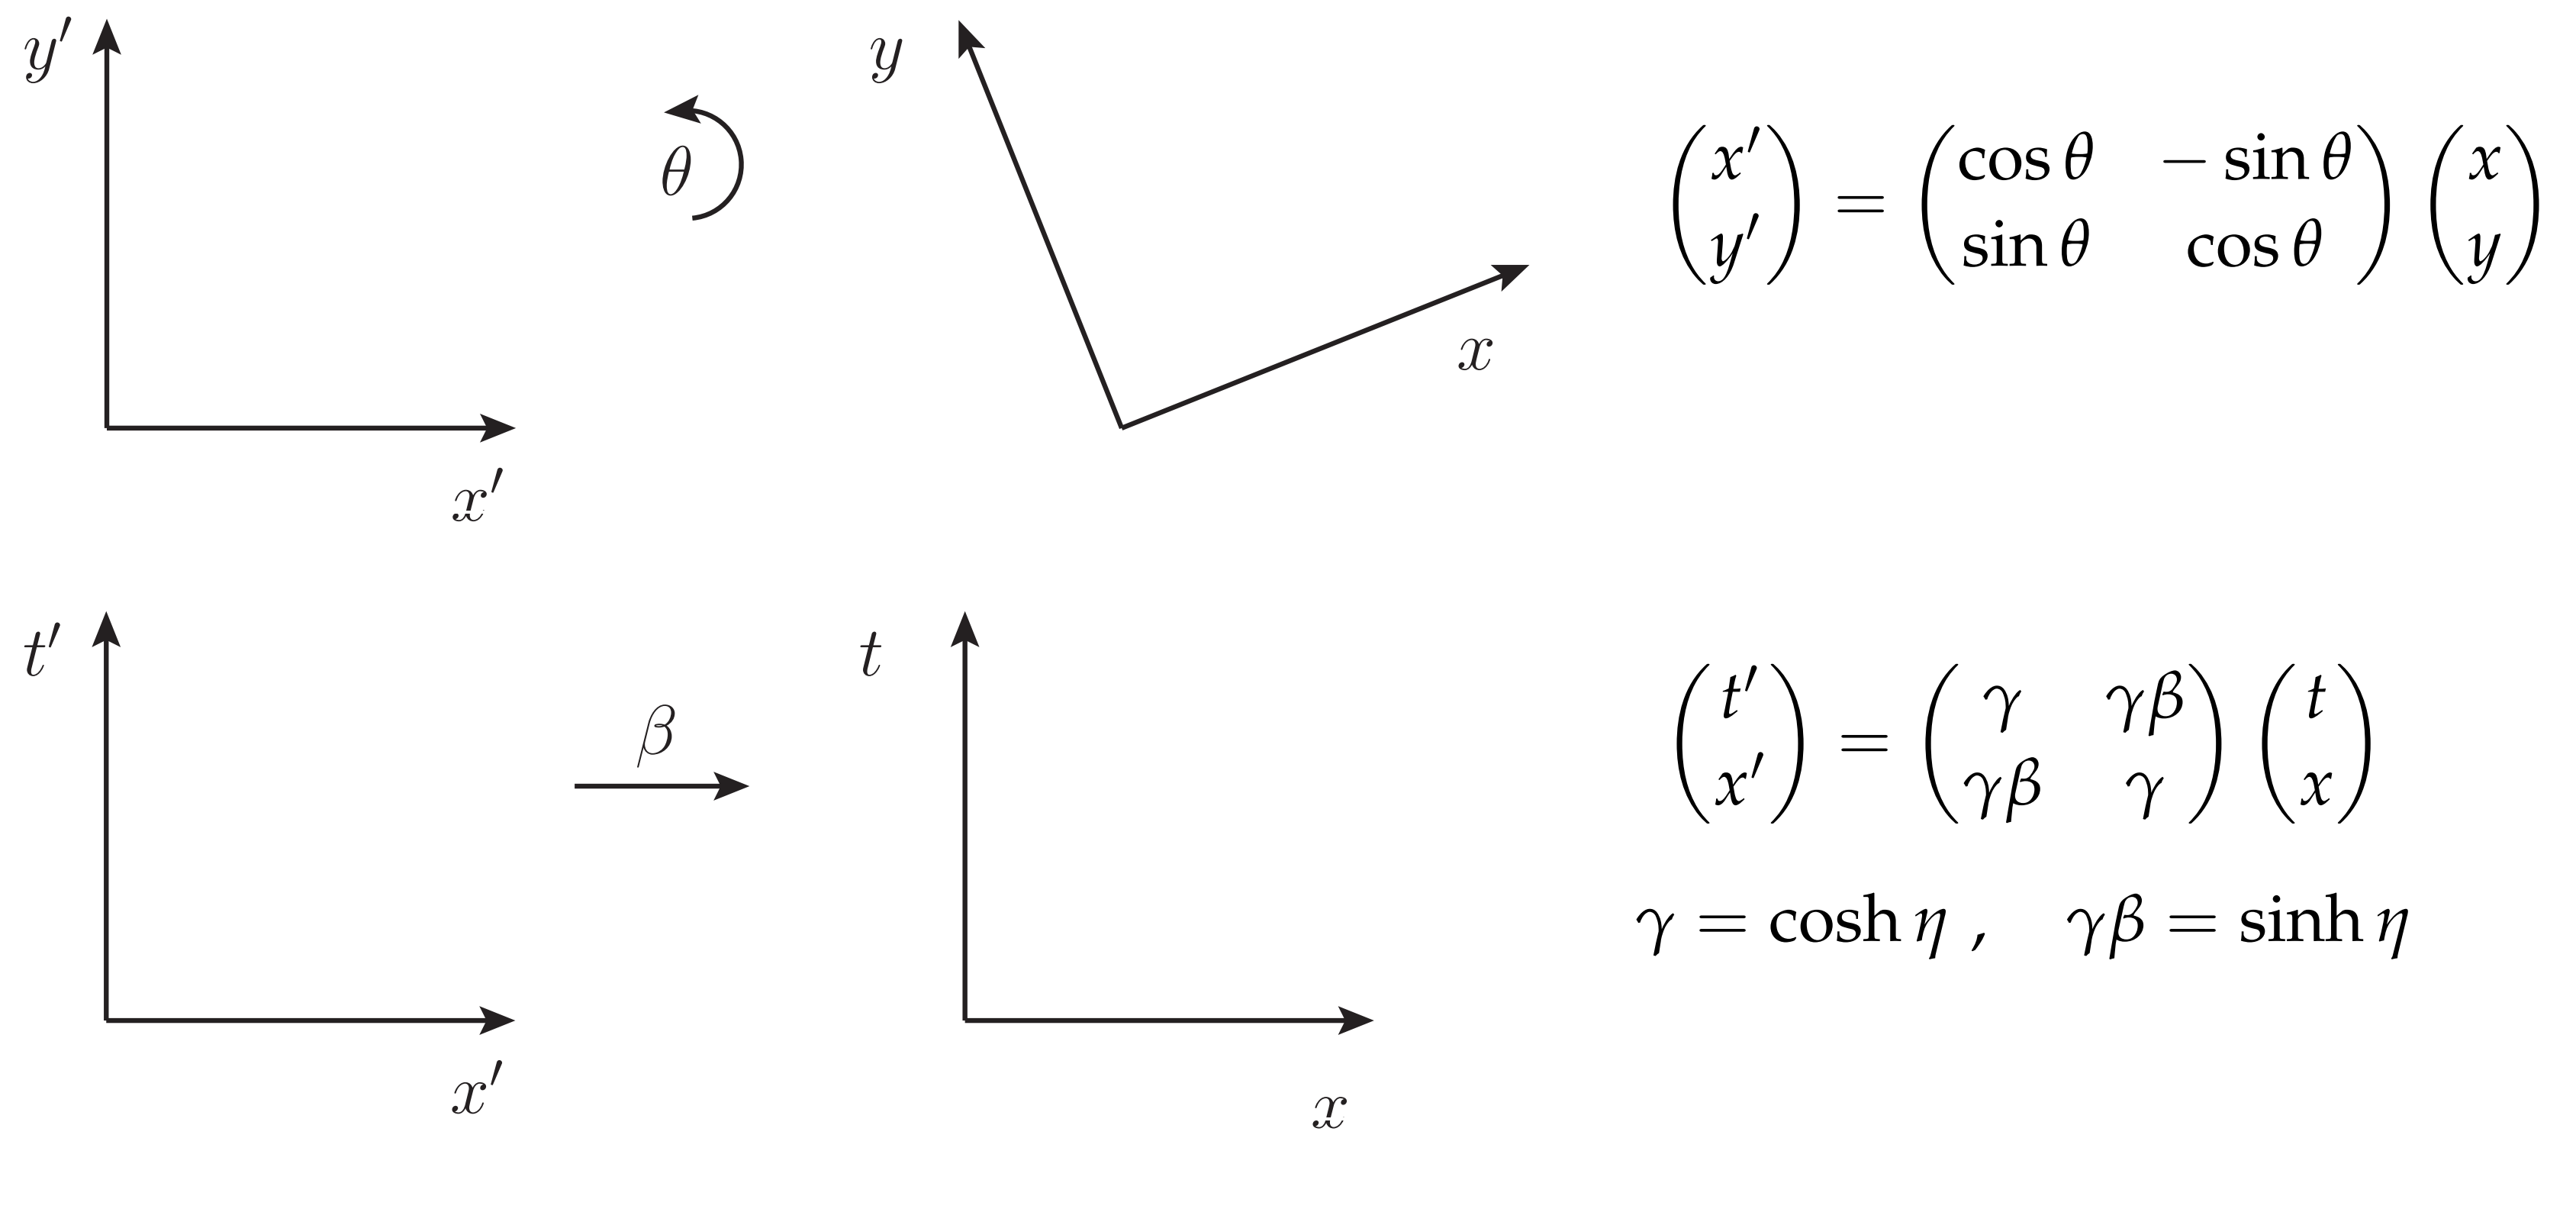
\includegraphics[scale=0.15]{Capitulos/Apendices/Ap_A3.png}
    \caption{Rotaciones y Boots}
%    \label{fig:my_label}
\end{figure}

Siguiendo la misma idea al grupo de rotaciones de $SO(3)$, algunos ejemplos de transformaciones de Lorentz. Por ejemplo las rotaciones al rededor de los ejes $x$, $y$ y $z$, son mediadas por las matrices:

\begin{equation}
    \left( \begin{array}{cccc}
    1 & 0 & 0 & 0 \\ 
    0 & 1 & 0 & 0 \\ 
    0 & 0 & \cos \theta _{x} & \sin \theta _{x} \\ 
    0 & 0 & -\sin \theta _{x} & \cos \theta _{x}
    \end{array} \right) ~,~\left( \begin{array}{cccc}
    1 & 0 & 0 & 0 \\ 
    0 & \cos \theta _{y} & 0 & -\sin \theta _{y} \\ 
    0 & 0 & 1 & 0 \\ 
    0 & \sin \theta _{y} & 0 & \cos \theta _{y}
    \end{array} \right) ~,~\left(  \begin{array}{cccc}
    1 & 0 & 0 & 0 \\ 
    0 & \cos \theta _{z} & \sin \theta _{z} & 0 \\ 
    0 & -\sin \theta _{z} & \cos \theta _{z} & 0 \\ 
    0 & 0 & 0 & 1
    \end{array}\right) ~.
    \label{rotaciones}
\end{equation}

También tenemos los boots en las direcciones $x$, $y$ y $z$

\begin{equation}
\left( 
\begin{array}{cccc}
\cosh \eta _{x} & \sinh \eta _{x} & 0 & 0 \\ 
\sinh \eta _{x} & \cosh \eta _{x} & 0 & 0 \\ 
0 & 0 & 1 & 0 \\ 
0 & 0 & 0 & 1
\end{array}
\right) ~,~\left( \begin{array}{cccc}
\cosh \eta _{y} & 0 & \sinh \eta _{y} & 0 \\ 
0 & 1 & 0 & 0 \\ 
\sinh \eta _{y} & 0 & \cosh \eta _{y} & 0 \\ 
0 & 0 & 0 & 1%
\end{array}
\right) ~,~\left( \begin{array}{cccc}
\cosh \eta _{z} & 0 & 0 & \sinh \eta _{z} \\ 
0 & 1 & 0 & 0 \\ 
0 & 0 & 1 & 0 \\ 
\sinh \eta _{z} & 0 & 0 & \cosh \eta _{z}
\end{array} \right) ~,
\label{boots}
\end{equation}
donde $\eta_{i}$ está relacionada con la velocidad $\beta_{i}=v_{i}$ del boost en la dirección $i$ por

\begin{equation*}
    \cosh \eta _{i}= \gamma_{i}=\frac{1}{\sqrt{1-v_{i}^{2}}}~,~\sinh \beta _{i}= \gamma_{i}\beta_{i} =\frac{v_{i}}{\sqrt{1-v_{i}^{2}}}~.
\end{equation*}
%~~\text{Aqui el doble índice no implica suma.}
Por otro lado, la reflexión total
\begin{equation}
\left( \begin{array}{cccc}
-1 & 0 & 0 & 0 \\ 
0 & -1 & 0 & 0 \\ 
0 & 0 & -1 & 0 \\ 
0 & 0 & 0 & -1
\end{array}\right)
~,
\end{equation}
 es también una transformación de Lorentz, así como lo es la inversión temporal
\begin{equation}
\left(\begin{array}{cccc}
-1 & 0 & 0 & 0 \\ 
0 & 1 & 0 & 0 \\ 
0 & 0 & 1 & 0 \\ 
0 & 0 & 0 & 1
\end{array}\right)~.
\end{equation}

La elección de los ejemplos que mostramos no es aleatoria: cualquier transformación de Lorentz puede descomponerse como un producto de estos cuatro tipos de transformaciones.\\

Las matrices de los ejemplos anteriores dan una representación del grupo de Lorentz sobre $\mathbb{C}^{4}$.\\
Aquí vamos a hacer un estudio más general de las representaciones del grupo de Lorentz y para ello estudiaremos su álgebra de Lie. Pero antes de eso, se hablará un poco acerca de la estructura de este grupo.

\subsubsection{Componentes del grupo de Lorentz}

Al tomar el determinante de ambos miembros de la ecuación (\ref{eqA31}) se obtiene:
\begin{equation}
    \det (\Lambda) = \pm 1~,
\end{equation}
esto define dos sub conjuntos de las transformaciones de Lorentz:
\begin{itemize}
    \item \textbf{Transformaciones Propias} si $\det (\Lambda) = +1$
    \item \textbf{Transformaciones Impropias} si $\det (\Lambda) = -1$
\end{itemize}

Ejemplos de transformaciones propias son: \emph{la identidad, las rotaciones, la reflexión total}. Mientras que la \emph{reflexión espacial} es un ejemplo de transformación impropia.\\

Hay una clasificación adicional dentro del grupo de Lorentz, que sale de escribir la componente $00$ de la ecuación (\ref{eqA31})

\begin{equation}
    (\Lambda^{0}_{0})^{2}-\sum_{j=1}^{3}(\Lambda^{j}_{0})^{2}=1~ \implies \qty(\Lambda^{0}_{~0})^{2} \geq 0 ~~\implies~\Lambda^{0}_{0} \geq 1 ~~ \text{ó} ~~ \Lambda^{0}_{0}  \leq -1~.
\end{equation}

\begin{minipage}[b]{0.7 \textwidth}
    El grupo de Lorentz consiste de cuatro componentes conexas (Ver figura \ref{Grupo de Lorentz}).\\

    \begin{itemize}
        \item [] $L_{+}^{\uparrow}$:  $\det \Lambda = + 1 ~~ \Lambda^{0}_{0} \geq 1$
        \item [] $L_{+}^{\downarrow}$:  $\det \Lambda = + 1 ~~ \Lambda^{0}_{0} \leq -1$
        \item [] $L_{-}^{\uparrow}$:  $\det \Lambda = - 1 ~~ \Lambda^{0}_{0} \geq 1$
        \item [] $L_{-}^{\uparrow}$:  $\det \Lambda = - 1 ~~ \Lambda^{0}_{0} \leq -1$
    \end{itemize}

\end{minipage}
\begin{minipage}[b]{0.3 \textwidth}
    \begin{figure}[H]
        \centering
        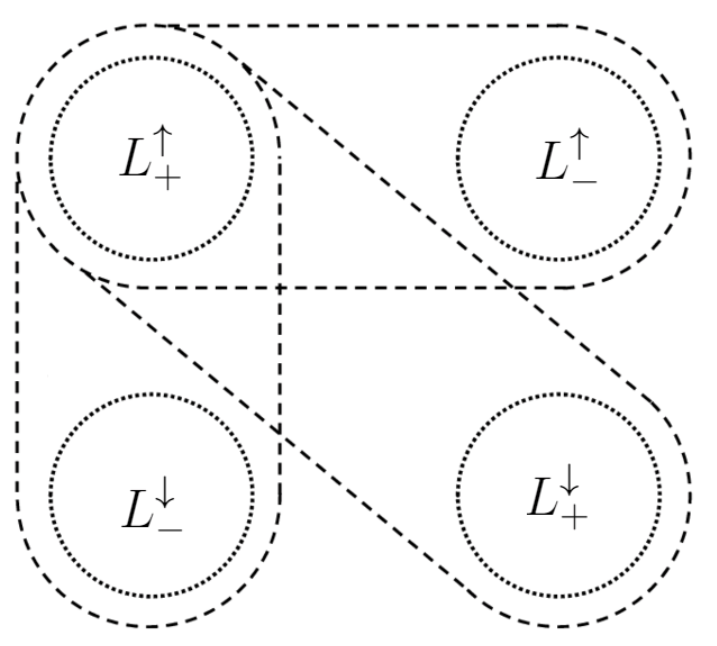
\includegraphics[width = 2.5cm]{Capitulos/Apendices/Ap_A.png}
        \caption{}
        \label{Grupo de Lorentz}
    \end{figure}
\end{minipage}

Las cuatro componentes conexas del grupo de Lorentz se esquematizan con círculos punteados en la figura, mientras que las líneas de trazos encierran a los tres subgrupos del grupo de Lorentz (note que todo grupo debe contener a $L_{+}^{\uparrow}$ ya que dicha componente es la que contiene a la identidad). El subgrupo $L_{+}^{\uparrow} \cup L_{+}^{\downarrow}$ se conoce como Grupo de Lorentz propio y se denota por $SO(3,1)$ y es el relevante para toda la fenomenología de partículas. (El $3$ por la dimensión espacial, el $1$ por la temporal). En detalle se tiene

\begin{enumerate}
    \item \textbf{Ortocronas} $(\Lambda^{0}_{0} \geq 1)$ \textbf{propias} ($\det \Lambda = + 1$)\\
    
    Forman grupo y es isomorfo a $SO(3,1)$. En adelante a $L_{+}^{\uparrow}$ lo llamaremos ``\emph{grupo de Lorentz propio ortocrono}''. Sus elementos son transformaciones continuas (grupo de Lie) que se pueden conectar con la identidad mediante sucesivas transformaciones infinitesimales. Sus elementos son rotaciones en las tres dimensiones espaciales y boosts (transformaciones de Lorentz puras). Estas últimas relacionan los sistemas de coordenadas de dos observadores inerciales (que se mueven con velocidad relativa constante).\\

    Las demás transformaciones obviamente no forman grupo y se pueden escribir como producto de inversiones (transformaciones discretas) y transformaciones de Lorentz ortocronas propias $\Lambda_{P}$. Estas son:
    \vspace{1cm}
    \item \textbf{No ortocronas} ($\Lambda^{0}_{0} \leq -1$) \textbf{propias} ($\det \Lambda = + 1$)   \\

    Transformaciones tipo $\Lambda_{P} \times \qty{\text{diag} \qty(-,-,-,-),~ \text{diag} \qty(-,-,+,+),~ \text{diag} \qty(-,+,-,+),~ \text{diag} \qty(-,+,+,-)}$. Incluye a las inversiones totales, $\text{diag} (-,-,-,-)$.
   \vspace{1cm} 
   \item  \textbf{Ortocronas} $(\Lambda^{0}_{0} \geq 1)$ \textbf{impropias} ($\det \Lambda = - 1$)\\

   Transformaciones tipo $\Lambda_{P} \times \qty{\text{diag} \qty(+,+,+,-),~ \text{diag} \qty(+,+,-,+),~ \text{diag} \qty(+,-,+,+),~ \text{diag} \qty(+,-,-,-)}$. Incluye a las inversiones espaciales, $\text{diag} (+,-,-,-)$.
   \vspace{1cm} 
   \item \textbf{No ortocronas} ($\Lambda^{0}_{0} \leq -1$) \textbf{impropias} ($\det \Lambda = - 1$)   \\
   Transformaciones tipo $\Lambda_{P} \times \qty{\text{diag} \qty(-,-,-,+),~ \text{diag} \qty(-,-,+,-),~ \text{diag} \qty(-,+,-,-),~ \text{diag} \qty(-,+,+,+)}$. Incluye a las inversiones temporales, $\text{diag} (-,+,+,+)$.
\end{enumerate}


%El subgrupo $L_{+}^{\uparrow}$ se conoce como \emph{Grupo de Lorentz propio ortócrono}. Sin embargo, este no es el único subgrupo de grupo de Lorentz. De hecho, $L_{+}^{\uparrow}$ junto a cualquiera de las otras tres componentes son subgrupos. El que también nos va a interesar $L_{+}^{\uparrow} \cup L_{+}^{\downarrow}$, que se conoce como Grupo de Lorentz propio, se denota por $SO(3,1)$ y es el relevante para toda la fenomenología de partículas. (El $3$ por la dimensión espacial, el $1$ por la temporal).\\

\vspace{0.4cm}
Observe que si queremos ver cuantos parámetros tiene el grupo de Lorentz (de transformaciones ortocronas propias), consideramos una transformación infinitesimal arbitraria 
\begin{equation}
    \Lambda^{\mu}_{~\nu}=\delta^{\mu}_{\nu}+\omega^{\mu}_{~\nu}
\end{equation}
donde (\ref{eqA31}) implica que $\omega_{\mu \nu}=-\omega_{\nu \mu}$.\\

Siendo $\omega$ antisimétrica tiene solamente 6 parámetros independientes, lo que en efecto garantiza que cualquier $\Lambda$ puede escribirse como producto de rotaciones $(R)$ Parametrizadas con 3 ángulos $\theta \in [0,2\pi]$ (ver eq. \ref{rotaciones}), y boots $(L)$ que se parametrizan especificando las tres componentes de la velocidad $\beta \in [-1,1]$ (ó $\eta \in [-\infty,\infty]$) a lo largo de $x$, $y$ o $z$ (ver eq. \ref{boots}).  



\subsection{Álgebra del grupo de Lorentz}

En esta sección, vamos a encontrar los generadores de las rotaciones y los boosts, y los conmutadores entre dichos generadores. Como las relaciones de conmutación valen lo mismo en cualquier representación (recuerde por ejemplo lo que vimos sobre las representaciones de $su(2)$) al hacer esto vamos a tener determinada en forma abstracta el álgebra del grupo de Lorentz. Una vez que se tenga el álgebra, será cuestión de estudiar sus representaciones para ver las que se inducen sobre el grupo.\\

A modo de ejemplo, calculemos el generador de los boots en la dirección $x$. Recuerde que dichos boots se representan por la siguiente matriz:

\begin{equation}
\Lambda \left( \eta _{x}\right) =\left( 
\begin{array}{cccc}
\cosh \eta _{x} & \sinh \eta _{x} & 0 & 0 \\ 
\sinh \eta _{x} & \cosh \eta _{x} & 0 & 0 \\ 
0 & 0 & 1 & 0 \\ 
0 & 0 & 0 & 1
\end{array}
\right)~. 
\end{equation}

Ahora, buscamos una matriz $M_{tx}=-M_{xt}$ tal que resulte
\begin{equation}
    \Lambda \qty(\eta_{x}) = e ^ {\frac{i}{2} \qty(\eta_{x}M^{tx}-\eta_{x}M^{xt})}  = e^{i\eta_{x}M^{tx}}~.
    \label{eqA_42}
\end{equation}

Aquí $\eta_{x}$ juega el rol análogo de los $\omega^{IJ}$ de la ecuación (\ref{A8}). Por ese motivo $M_{xt}$ aparece multiplicado por $-\eta_{x}$, que recuerde que $\omega^{IJ}=\omega^{JI}$. Agregamos además la unidad imaginaria $i$ para ser consistentes con la definición más común de los generadores que suele hacerse en la literatura de física. En virtud de la ecuación (\ref{eqA_42}) se tiene que cumplir que 
\begin{equation}
    M^{tx} = -i \eval{\dv{\Lambda (\eta_{x})}{\eta_{x}}}_{\eta_{x} = 0}~, 
\end{equation}
que introduciendo la forma explicita de boost nos da
\begin{equation}
\begin{split}
    M^{tx} &= -i \eval{\dv{\Lambda (\beta_{x})}{\beta_{x}}}_{\beta_{x} = 0} \\
    &= -i\left(  \begin{array}{cccc}
    0 & 1 & 0 & 0 \\ 
    1 & 0 & 0 & 0 \\ 
    0 & 0 & 0 & 0 \\ 
    0 & 0 & 0 & 0 
    \end{array} \right) ~.
\end{split}
\end{equation}

Siguiendo un proceso similar se puede obtener los generadores asociados a los boots en $y$ t $z$:
\begin{equation}
    M^{ty}=-i\left(  \begin{array}{cccc} 
    0 & 0 & 1 & 0 \\ 
    0 & 0 & 0 & 0 \\ 
    1 & 0 & 0 & 0 \\ 
    0 & 0 & 0 & 0 
    \end{array} \right) ~,~\ M^{tz}=-i\left( \begin{array}{cccc}
    0 & 0 & 0 & 1 \\ 
    0 & 0 & 0 & 0 \\ 
    0 & 0 & 0 & 0 \\ 
    1 & 0 & 0 & 0
    \end{array}
\right) ~,
\end{equation}
 y los asociados a las rotaciones en $x$, $y$ y $z$

 \begin{equation}
M^{yz}=-i\left( 
\begin{array}{cccc}
0 & 0 & 0 & 0 \\ 
0 & 0 & 0 & 0 \\ 
0 & 0 & 0 & 1 \\ 
0 & 0 & -1 & 0
\end{array}
\right) ~,~\ M^{zx}=-i\left( 
\begin{array}{cccc}
0 & 0 & 0 & 0 \\ 
0 & 0 & 0 & -1 \\ 
0 & 0 & 0 & 0 \\ 
0 & 1 & 0 & 0
\end{array}
\right) ~,~\ M^{xy}=-i\left( 
\begin{array}{cccc}
0 & 0 & 0 & 0 \\ 
0 & 0 & 1 & 0 \\ 
0 & -1 & 0 & 0 \\ 
0 & 0 & 0 & 0
\end{array}
\right) ~.
\end{equation}

Note que, salvo por la dimensión y por el factor $-i$ asociado al cambio de definición, los generadores de las rotaciones tienen la misma forma ya encontradas en las ecuaciones (\ref{eqA_18}) y (\ref{eqA_19}). Puede corroborarse que se cumple:
\begin{equation}
    \comm{M^{\mu \nu}}{M^{\rho \sigma}} = i \qty(g^{\mu \sigma}M^{\nu \rho} + g^{\nu \rho}M^{\mu \sigma} - g^{\mu \rho}M^{\nu \sigma}-g^{\nu \sigma}M^{\mu \rho} )~,
    \label{alorentz}
\end{equation}
haciendo los conmutadores entre las matrices (No olvide que los subíndices aquí etiquetan a las matrices y no denotan componentes). Esta es el álgebra del grupo de Lorentz propio y se denota por $so(3,1)$.\\

Tenga presenta también que, como la variedad paramétrica de los boots no es compacta, sus generadores no son hermíticos. Ya con el álgebra de Lorentz, se analizará unos desarrollos que nos permitirán escribir las representaciones de $so(3,1)$ en términos de representaciones de $su(2)$. Para ello primero, veamos una forma de reescribir las relaciones entre los generadores $M_{\mu \nu}$ que definen el álgebra de Lorentz. Definimos

\begin{eqnarray}
J^{i} &\equiv &\frac{1}{2}\epsilon ^{ijk}M^{jk}~\Longrightarrow ~\left\{ 
\begin{array}{c}
J^{1}=M^{23}=-M^{32} \\ 
J^{2}=M^{31}=-M^{13} \\ 
J^{3}=M^{12}=-M^{21}
\end{array}
\label{eqA_1.36}
\right.  \\
K^{i} &\equiv &M^{i0}=-M^{0i}
\label{eqA_1.37}
\end{eqnarray}

%\begin{equation}
%    J_{i} \equiv \frac{1}{2} \epsilon_{ijk} M_{jk}~,
%    K_{i} \equiv M_{i0}~,
%\end{equation}
donde $i,j,k$ hacen referencia a la parte espacial. Así:

\begin{eqnarray}
J^{1} &=&\left( 
\begin{array}{cccc}
0 & 0 & 0 & 0 \\ 
0 & 0 & 0 & 0 \\ 
0 & 0 & 0 & -i \\ 
0 & 0 & i & 0%
\end{array}%
\right) ~\ ,~\ \ J^{2}=\left( 
\begin{array}{cccc}
0 & 0 & 0 & 0 \\ 
0 & 0 & 0 & i \\ 
0 & 0 & 0 & 0 \\ 
0 & -i & 0 & 0%
\end{array}%
\right) ~\ ,~\ \ J^{3}=\left( 
\begin{array}{cccc}
0 & 0 & 0 & 0 \\ 
0 & 0 & -i & 0 \\ 
0 & i & 0 & 0 \\ 
0 & 0 & 0 & 0%
\end{array}%
\right)  \\
K^{1} &=&\left( 
\begin{array}{cccc}
0 & i & 0 & 0 \\ 
i & 0 & 0 & 0 \\ 
0 & 0 & 0 & 0 \\ 
0 & 0 & 0 & 0%
\end{array}%
\right) ~\ ,~\ K^{2}=\left( 
\begin{array}{cccc}
0 & i & 0 & 0 \\ 
i & 0 & 0 & 0 \\ 
0 & 0 & 0 & 0 \\ 
0 & 0 & 0 & 0%
\end{array}%
\right) ~\ ,~\ K^{3}=\left( 
\begin{array}{cccc}
0 & 0 & 0 & i \\ 
0 & 0 & 0 & 0 \\ 
0 & 0 & 0 & 0 \\ 
i & 0 & 0 & 0%
\end{array}%
\right) 
\end{eqnarray}

Es bien conocido que los generadores de las rotaciones cumplen que 
\begin{equation}
    \comm{J^{i}}{J^{j}} = i \epsilon^{ijk}J^{k}~,
\end{equation}
indicándonos que el álgebra asociada al grupo de rotaciones es $su(2)$. Veamos ahora los otros conmutadores, comenzando por el de dos boost:

\begin{eqnarray*}
\left[ K^{i},K^{j}\right]  &=&\left[ M^{i0},M^{j0}\right]  \\
&=&i\left( g^{i0}M^{0j}+g^{oj}M^{io}-g^{ij}M^{00}-g^{00}M^{ij}\right)  \\
&=&i\left( -g^{00}M^{ij}\right) .
\end{eqnarray*}

Usando que $M^{ij}=-M^{ji}$, se puede reescribir $M^{ij}$ como $\left(M^{ij}-M^{ji}\right) /2$. Entonces

\begin{equation}
\left[ K^{i},K^{j}\right] =-i\left[ \frac{1}{2}\left( M^{ij}-M^{ji}\right) 
\right] =-i\epsilon ^{kij}J^{k}
\end{equation}

donde se ha usado que $J_{k}\epsilon _{kmn}=\frac{1}{2}\left(M_{mn}-M_{nm}\right) $, relaci\'{o}n que se puede probar empleando la propiedad $\epsilon _{ijk}\epsilon _{imn}=\delta _{jm}\delta _{kn}-\delta_{jn}\delta _{km}$. Vemos entonces que los generadores de boost no conmutan entre si. De forma análoga se puede calcular el conmutador restante entre generadores de boost y rotaciones. En resumen se tiene que el álgebra de lie es:

\begin{equation}
    \comm{J^{i}}{J^{j}}=i\epsilon^{ijk}J^{k}~,~~\comm{K^{i}}{K^{j}}=-i\epsilon^{ijk}J^{k}~,~~\comm{J^{i}}{K^{j}}=i\epsilon^{ijk}K^{k}   ~.     
\end{equation}

Note que las relaciones anteriores permiten concluir que los boost no forman un grupo ya que el álgebra de sus generadores no es cerrada, a diferencia de lo que sucede con las rotaciones.\\

Conviene ahora definir:
\begin{equation}
    \bar{A}\equiv \frac{1}{2} \qty(\bar{J}-i\bar{K})~,~~ \bar{B}\equiv \frac{1}{2} \qty(\bar{J}+i\bar{K})~,
\end{equation}
siendo $\bar{J}=(J^{1},J^{2},J^{3})$ y $\bar{K}=(K^{1},K^{2},K^{3})$, el álgebra de Lorentz es ahora una suma directa de dos $su(2)$. Para ver esto, hallemos los conmutadores entre estos nuevos generadores

\begin{eqnarray}
\left[ A^{i},A^{j}\right]  &=&\left[ \frac{1}{2}\left( J^{i}-iK^{i}\right) ,
\frac{1}{2}\left( J^{j}-iK^{j}\right) \right]   \notag \\
&=&\frac{1}{4}\left( \left[ J^{i},J^{j}\right] -i\left[ K^{i},J^{j}\right] -i
\left[ J^{i},K^{j}\right] -\left[ K^{i},K^{j}\right] \right)   \notag \\
&=&\frac{1}{4}\left( i\epsilon ^{ijk}J^{k}+\epsilon ^{ijk}K^{k}+\epsilon
^{ijk}K^{k}+i\epsilon ^{ijk}J^{k}\right) =\frac{i\epsilon ^{ijk}}{2}\left(
J^{k}-iK^{k}\right)   \notag \\
&=&i\epsilon ^{ijk}A^{k}~.
\end{eqnarray}%
\begin{eqnarray}
\left[ B^{i},B^{j}\right]  &=&\left[ \frac{1}{2}\left( J^{i}+iK^{i}\right) ,
\frac{1}{2}\left( J^{j}+iK^{j}\right) \right]   \notag \\
&=&\frac{1}{4}\left( \left[ J^{i},J^{j}\right] +i\left[ J^{i},K^{j}\right] +i
\left[ K^{i},J^{j}\right] -\left[ K^{i},K^{j}\right] \right)   \notag \\
&=&\frac{1}{4}\left( i\epsilon ^{ijk}J^{k}-\epsilon ^{ijk}K^{k}-\epsilon
^{ijk}K^{k}+i\epsilon ^{ijk}J^{k}\right) =\frac{i\epsilon ^{ijk}}{2}\left(
J^{k}+iK^{k}\right)   \notag \\
&=&i\epsilon ^{ijk}B^{k}~.
\end{eqnarray}

\begin{eqnarray}
\left[ A^{i},B^{j}\right]  &=&\left[ \frac{1}{2}\left( J^{i}-iK^{i}\right) ,
\frac{1}{2}\left( J^{j}+iK^{j}\right) \right]   \notag \\
&=&\frac{1}{4}\left( \left[ J^{i},J^{j}\right] +i\left[ J^{i},K^{j}\right] -i
\left[ K^{i},J^{j}\right] +\left[ K^{i},K^{j}\right] \right)   \notag \\
&=&\frac{1}{4}\left( i\epsilon ^{ijk}J^{k}-\epsilon ^{ijk}K^{k}+\epsilon
^{ijk}K^{k}-i\epsilon ^{ijk}J^{k}\right)   \notag \\
&=&0~.
\end{eqnarray}

Vemos entonces que los operadores $A_{i}$ y $B_{i}$ conmutan entre ellos, es decir sus álgebras son independientes entre sí, y además, el álgebra de cada uno de ellos es el álgebra $su(2)$. En términos matemáticos, $so(3,1) = su(2) \oplus su(2)$ y es localmente isomorfo a $SU(2)\times SU(2)$ por tener la misma álgebra. De esta propiedad para el álgebra de Lie correspondiente al grupo de Lorentz se desprende que 

\begin{cabox}
    Las representaciones Lorentz irreducibles se puedan etiquetar por el par de semi-enteros $(j_{1},j_{2})$ de dimensión $(2j_{1}+1)(2j_{2}+1)$, que corresponden al espín de la representación de cada $su(2)$.
\end{cabox}

Notese que hemos encontrado irreps del grupo de Lorentz de dimensión finita, pero no son unitarias porque no es compacto.

%--------------------------------
otra forma de escribir los generadores del grupo de Lorentz es la siguiente. Tomamos como parámetros los $6$ elementos independientes de una matriz antisimétrica $\omega_{\mu \nu}=-\omega_{\nu \mu}$. Los generadores son entonces las $6$ componentes independientes del operador antisimétrico $M^{\mu \nu}=-M^{\nu \mu}$,
\begin{equation}
    \Lambda = e^{-\frac{i}{2}\omega_{\mu\nu}M^{\mu \nu}}~,
    \label{eqA1_2.19}
\end{equation}
(el factor $1/2$ compensa el hecho que sumaos sobre $\mu,\nu$). Al definir $\theta$ y $\eta$ mediante
\begin{eqnarray}
\theta ^{k} &=&\frac{1}{2}\epsilon ^{klm}\omega ^{lm}~\Rightarrow ~\left\{ 
\begin{array}{c}
\theta ^{1}=\omega ^{23}=-\omega ^{32}=\omega _{23}=-\omega _{32} \\ 
\theta ^{2}=\omega ^{31}=-\omega ^{13}=\omega _{31}=-\omega _{13} \\ 
\theta ^{3}=\omega ^{12}=-\omega ^{21}=\omega _{12}=-\omega _{21}
\end{array}
\right.  \\
\eta ^{k} &=&\omega ^{0k}=-\omega ^{k0}=-\omega _{0k}=\omega _{k0}
\end{eqnarray}
tenemos que,
\begin{equation}
\begin{split}
    \frac{1}{2}\omega_{\mu \nu}M^{\mu \nu} &=  \omega_{12}M^{12}+\omega_{31}M^{31}+\omega_{23}M^{23}+\omega_{i0}M^{i0} \\
    & = \theta^{i}J^{i} + \eta^{i}K^{i}  \\
    & \equiv \vb*{\theta} \cdot \vb{J} + \vb*{\eta} \cdot \vb{K}~,  
\end{split}
\end{equation}
por lo que
\begin{equation}
    \Lambda=\ee^{-i\qty(\vb*{\theta} \cdot \vb{J} + \vb*{\eta} \cdot \vb{K}) }~,
    \label{eqA_71}
\end{equation}
Observe que 
\begin{equation}
    \Lambda^{-1}=\ee^{i\qty(\vb*{\theta} \cdot \vb{J} + \vb*{\eta} \cdot \vb{K}) } \neq \Lambda^{\dagger}=\ee^{i\qty(\vb*{\theta} \cdot \vb{J} - \vb*{\eta} \cdot \vb{K}) }
\end{equation}

lo que quiere decir que las irreps del grupo de Lorentz de dimensión finita no son unitarias, porque no es compacto. Al redefinir $M^{\mu \nu}\equiv J^{\mu \nu}$, se tiene que su representación es una matriz $4\times 4$ $(J^{\mu \nu})^{\rho}_{~\sigma}$.\\

La forma explicita de estos generadores es

\begin{equation}
    (J^{\mu \nu})^{\rho}_{~\sigma} = i \qty(g^{\mu \rho} \delta^{\nu}_{~\sigma}-g^{\nu \rho} \delta^{\mu}_{~\sigma})~,
    \label{eqA2.32}
\end{equation}
  los cuales satisfacen el álgebra de Lie dada en (\ref{eq_A106})-

\subsection{Representaciones Tensoriales}

Lo que acabamos de ver es la representación en cuatro dimensiones del grupo de Lorentz, que nos ha servido para definir el grupo. Podemos plantearnos si es irreducible (lo es) y si es su representación no trivial de dimensión más pequeña (veremos que no lo es). Se llama representación vectorial del grupo de Lorentz:

\begin{equation}
    \Lambda^{\mu}_{~\nu}=\qty\bigg[e^{-i\qty(\vb*{\theta} \cdot \vb{J} + \vb*{\eta} \cdot \vb{K}) }]^{\mu}_{~\nu}=~\qty\bigg[e^{-i\qty(\frac{1}{2} \omega_{\alpha \beta}J^{\alpha \beta})}]^{\mu}_{~\nu},
\end{equation}

Un cuadrivector contravariante $V^{\mu}$ (ó covariante $V_{\mu}$) es un vector que pertenece a un espacio vectorial invariante e irreducible que se transforma como
\begin{equation}
    V^{\mu \prime}=\Lambda^{\mu}_{~\nu} V^{\nu}~~,~~V_{\mu \prime}=\Lambda_{\mu}^{~\nu} V_{\nu}~,
 \end{equation}
 donde $\Lambda^{\mu}_{~\nu}$ y $\Lambda_{\mu}^{~\nu}$ son representaciones equivalentes, dado que están relacionadas mediante una transformación de semejanza $S=g_{\mu \nu}$ tal que $\Lambda^{\mu}_{~\nu}=g^{\mu \rho}\Lambda_{\rho}^{~\sigma}g_{\sigma \nu}$.\\

 Se debe tener en cuenta que el término representación se asocia con el espacio de representación. Así diremos que $V^{\mu}$ y $V_{\mu}$ son irreps equivalentes. $V_{\mu}$ es el vector asociado a $V^{\mu}$ en el espacio dual, así que la matriz $\Lambda_{\mu}^{~\nu}$ es la inversa de $\Lambda^{\mu}_{~\nu}$, dado que de ((\ref{eqA31}): $g_{\mu \nu }=\Lambda _{~\mu }^{\alpha }\Lambda _{~\nu }^{\beta}g_{\alpha \beta }$)
 
\begin{eqnarray*}
g_{\alpha \beta }\Lambda _{~\mu }^{\alpha }\Lambda _{~\nu }^{\beta }
&=&\Lambda _{\beta \mu }\Lambda _{~\nu }^{\beta }=g_{\mu \nu }, \\
g_{\alpha \beta }\Lambda _{~\mu }^{\alpha }\Lambda _{~\nu }^{\beta }
&=&\Lambda _{~\mu }^{\alpha }\Lambda _{\alpha \nu }=g_{\mu \nu },
\end{eqnarray*}%
y multiplicando la primera linea anterior por $g^{\tau \mu }$%
\begin{eqnarray}
g^{\tau \mu }\Lambda _{\beta \mu }\Lambda _{~\nu }^{\beta } &=&g^{\tau \mu
}g_{\mu \nu }~\Longrightarrow ~\Lambda _{\beta }^{~\tau }\Lambda _{~\nu
}^{\beta }=g^{\tau \mu }g_{\mu \nu }=g_{~\nu }^{\tau }~,  \notag \\
&\therefore &~\Lambda _{\beta }^{~\mu }\Lambda _{~\nu }^{\beta }=g_{~\nu
}^{\mu }=\delta _{\nu }^{\mu }~.
\end{eqnarray}
 
Se pueden construir representaciones de dimensiones mayores mediante el producto tensorial. A estas representaciones se llaman tensoriales y sus vectores son tensores con varios índices (Su número se llama rango). Así, un tensor $T^{\mu \nu}$ on dos índices contravariantes es un objeto que transforma bajo Lorentz como:
\begin{equation}
    T^{\mu \nu} = \Lambda^{\mu}_{~\mu^{\prime}} \Lambda^{\nu}_{~\nu^{\prime}} T^{\mu^{\prime} \nu^{\prime}}~.
\label{eqA2.34}
\end{equation}

En general, un tensor con índices arriba transforma con $\Lambda^{\mu}_{~\nu}$, y con índices abajo transforma con $\Lambda_{\mu}^{~\nu}$.\\

Los tensores son ejemplos de representaciones del grupo de Lorentz, por ejemplo $T^{\mu}_{~\nu}$ con dos índices contravariantes tiene $4^{2}=16$ componentes, las cuales constituyen la base para una representación en dimensión 16. Sin embargo, esta representación es reducible, dado que de la ecuación (\ref{eqA2.34}) se observa que, si $T^{\mu}_{~\nu}$ es antisimétrico, después de una transformación de Lorentz permanece antisimétrico, al igual que si es simétrico entonces permanece simétrico. Esto quiere decir que las partes simétrica y antisimétrica del tensor no se mezclan y por tanto la representación en 16 dimensiones es reducible a una rep. de 6 dimensiones antisimétrica $A^{\mu \nu}=(1/2)(T^{\mu \nu}-T^{\nu \mu})$, y una rep. de 10 dimensiones simétrica $S^{\mu \nu}=(1/2)(T^{\mu \nu}+T^{\nu \mu})$.

La traza de un tensor se define como 
\begin{equation}
    S \equiv S^{\mu}_{~\mu}=g_{\mu \nu}S^{\mu \nu} ~~\implies~~ S^{\prime}=S^{ \prime \mu}_{~\mu}=\Lambda^{\mu}_{~\rho}\Lambda_{\mu}^{~\sigma} S^{\rho}_{~\sigma}=\delta^{\sigma}_{\rho}S^{\rho}_{~\sigma} = S^{\rho}_{~\rho}=S~,
\end{equation}
 lo que demuestra que la traza de un tensor permanente invariante ante transformaciones de Lorentz. Por lo tanto, si se tiene un tensor sin traza, este permanecerá sin traza luego de una T.L. y por ende, la representación simétrica de 10 dimensiones se descompone aún más en una representación sin traza simétrica irreducible de dimensión 9, $S^{\mu \nu}-(1/4)g^{\mu \nu}S$ y la representación unidimensional (escalar) $S$. Este hecho verifica que un tensor de segundo orden pueda escribirse como una suma directa de representaciones irreducibles
 \begin{equation}
     \vb*{4} \otimes \vb*{4} = \vb*{1} \oplus \vb*{6} \oplus \vb*{9}~,
 \end{equation}
donde la representación irreducible es denotada por su dimensionalidad en negrita. Por lo tanto $\vb*{1}$ es la rep. escalar (Unidimensional), $\vb*{4}$ la rep. de un cuadrivector, $\vb*{6}$ el tensor antisimétrico y $\vb*{9}$ el tensor simétrico sin traza. De este modo cualquier tensor arbitrario se escribe como:
\begin{equation}
\begin{split}
    T^{\mu \nu} &= \frac{1}{2}g^{ \mu \nu}T+A^{\mu \nu} + S^{ \mu \nu}~,  \text{donde}\\
    T =& T^{\mu}_{~\mu}\\
    A^{\mu \nu} &=\frac{1}{2}\qty(T^{\mu \nu} - T^{\nu \mu})\\
    S^{\mu \nu} &=\frac{1}{2}\qty(T^{\mu \nu} + T^{\nu \mu})-\frac{1}{4}g^{\mu \nu}T
\end{split}
\end{equation}
 Por este mismo razonamiento, $T^{\mu}_{~\nu}$, $T_{\mu}^{~\nu}$ y $T_{\mu \nu}$ son representaciones (reducibles) equivalentes del grupo de Lorentz.\\

 Es interesante ver ver como se transforman las irrepsdel grupo de Lorentz bajo el sub grupo de las rotaciones.\\
 Como sabemos el comportamiento de un tensor bajo una transformación genérica de Lorentz, conocemos en particular sus propiedades de transformación bajo el subgrupo de rotación $SO(3)$, y por lo tanto nos podemos preguntar cuál es el momento angular $j$ de las diversas representaciones de tensor. Recuerde que las representaciones de $SO(3)$ están etiquetadas por un índice $j$ que toma valores enteros $j=1,2,\ldots,$ y la dimensión de la representación etiquetada por $j$ es $2j + 1$. Dentro de cada representación, estos $2j + 1$ estados están etiquetados por $j_{z}=-j,\ldots,j$. Para $SO(3)$, es más común denotar la representación como $\vb*{j}$, es decir, etiquetarla con el momento angular en lugar de con la dimensión de la representación, $2j+1$. En esta notación, $\vb*{0}$ es el escalar (también llamado el singlete), $\vb*{1}$ es un triplete con componentes $j_{z}=-1,0,1$, dimensión 5,... etc. (si preferimos usar la misma convención que en el caso del grupo de Lorentz, es decir, los etiquetamos por su dimensionalidad, deberíamos escribir $\vb*{1}$, $\vb*{3}$, $\vb*{5}$,...).\\

 Un escalar de Lorentz, por supuesto, también es escalar bajo rotaciones, por lo que tiene $j=0$. Un cuadrivector $V^{\mu}=(V^{0},\vb*{V})$ es una representación irreducible del grupo de Lorentz, ya que una transformación de Lorentz genérica mezcla los cuatro componentes, pero desde el punto de vista del subgrupo $SO(3)$ es reducible: las rotaciones espaciales no mezclan $V^{0}$ con $\vb*{V}$, por ende $V^{0}$ es invariante bajo rotaciones espaciales, por lo que tiene asociado espín $j = 0$, mientras que los tres componentes espaciales $V^{i}$ forman una representación tridimensional irreducible de $SO(3)$, por lo que tienen espín $j = 1$. En el lenguaje de la teoría de grupos decimos que, desde el punto de vista de las rotaciones espaciales, un cuadrivector se puede descomponer en la suma directa de un escalar y una representación $j = 1$,\\
 \begin{equation}
     V^{\mu} \in \vb*{0}\oplus \vb*{1} ~~ \text{etiquetadas por $j=0,1$ bajo el grupo de rotaciones}.
 \end{equation}

 Ahora queremos entender qué momentos angulares aparecen en un tensor genérico $T^{\mu \nu}$ con dos índices. Por definición, un tensor $T^{\mu \nu}$ se transforma como el producto tensorial de dos representaciones de cuadrivectores. Entonces desde el punto de vista del grupo de rotaciones $SO(3)$
 \begin{equation}
 \begin{split}
     T^{\mu \nu} \in \vb*{4} \otimes \vb*{4} &= \vb*{1} \oplus \vb*{6} \oplus \vb*{9} \\
     &= (\vb*{0} \oplus \vb*{1}) \otimes (\vb*{0} \oplus \vb*{1})\\
     &= (\vb*{0} \otimes \vb*{0}) \oplus (\vb*{0} \otimes \vb*{1}) \oplus (\vb*{1} \otimes \vb*{0}) \oplus (\vb*{1} \otimes \vb*{1})\\
     &= \vb*{0} \oplus \vb*{1} \oplus \vb*{1} \oplus ( \vb*{0} \oplus \vb*{1} \oplus \vb*{2} ) ~.
 \end{split} 
 \end{equation}

donde se ha usado que el producto directo de irreps del grupo de las rotaciones obedece la regla de adición de momento angular estableciendo que al componer dos momentos angulares,

\begin{equation}
    j_{1} \otimes j_{2} = \abs{j_{1}-j_{2}} \oplus \abs{j_{1}-j_{2}}+1 \oplus  \cdots  \oplus \cdots j_{1}+j_{2}-1  \oplus j_{1}+j_{2}~.
\end{equation}

Así, en la descomposición de un tensor arbitrario $T^{\mu \nu}$ en representaciones del grupo de rotación, corresponde a la suma directa de las irreps asociadas a $j = 0$ (aparece dos veces), $j = 1$ (aparece tres veces) y la $j = 2$ una vez. Explícitamente

\begin{eqnarray*}
\mathbf{1} &:&~~\ T\in ~\mathbf{0~~\ \ }~\text{(Es tambi\'{e}n un escalar bajo rotaciones)}  \notag \\
\mathbf{6} &:&~~\ A^{\mu \nu }\in ~\mathbf{1\oplus 1}~\ \mapsto ~\left\{ 
\begin{array}{c}
A^{0i} \\ 
\frac{1}{2}\epsilon ^{ijk}A^{jk}%
\end{array}%
\right. \text{ \ \ (Corresponde a dos 3-vectores independientes bajo
rotaciones.)} \\
\mathbf{9} &:&~~\ S^{\mu \nu }\in ~\mathbf{0\oplus 1\oplus 2}~\ \mapsto
~\left\{ 
\begin{array}{c}
S^{00} \\ 
S^{0i} \\ 
S^{ij}~\ \ ;~\ \sum\limits_{i}S^{ij}=-S^{00}
\end{array}
\right.   \notag
\end{eqnarray*}

En general, un tensor $T^{\mu \nu \rho \ldots} $ con $N$ componentes contiene espines $j=0,1,\ldots,N.$

Como curiosidad, un tensor completamente antisimétrico de orden $4$, $A^{\mu \nu \rho \sigma}$, solo tiene una componente diferente de cero $A^{0123}$, de modo que se puede escribir como $A^{\mu \nu \rho \sigma} = a\epsilon^{\mu \nu \rho \sigma}$, por lo tanto es un escalar de Lorentz pues

\begin{equation}
    \epsilon^{\mu \nu \rho \sigma} = \Lambda^{\mu}_{~\mu^{\prime}} \Lambda^{\nu}_{~\nu^{\prime}} \Lambda^{\rho}_{~\rho^{\prime}} \Lambda^{\sigma}_{~\sigma^{\prime}} \epsilon^{\mu^{\prime} \nu^{\prime} \rho^{\prime} \sigma^{\prime}}=\det(\Lambda)\epsilon^{\mu \nu \rho \sigma}=\epsilon^{\mu \nu \rho \sigma}~.
    \label{A_84}
\end{equation}
%    \epsilon^{\prime \mu \nu \rho \sigma}=\Lambda^{\mu}_{~\alpha}\Lambda^{\nu}_{~\beta}\Lambda^{\rho}_{~\tau}\Lambda^{\sigma}_{~\theta} \epsilon^{ \alpha \beta \tau \theta}.

Para entender esto, recuerde que el tensor de Levi-Civita permite escribir el determinante de $A^{\mu}_{~\nu}$ como:
\begin{equation}
    (\det A) \epsilon^{\mu \nu \rho \sigma} \equiv A_{~\alpha}^{\mu} A_{~\beta}^{\nu} A_{~\gamma}^{\rho} A_{~\delta}^{\sigma}\epsilon^{\alpha \beta \gamma \delta}~,
 \end{equation}
en particular, si $A=\Lambda$,
\begin{equation}
    \Lambda^{\mu}_{~\mu^{\prime}} \Lambda^{\nu}_{~\nu^{\prime}} \Lambda^{\rho}_{~\rho^{\prime}} \Lambda^{\sigma}_{~\sigma^{\prime}} \epsilon^{\mu^{\prime} \nu^{\prime} \rho^{\prime} \sigma^{\prime}} = \det(\Lambda) \epsilon^{\mu \nu \rho \sigma}~,
    \label{detL}
\end{equation}
donde el tensor de Levi-Civita bajo una transformación de Lorentz transforma como
\begin{equation}
    \epsilon^{\mu \nu \rho \sigma} = \Lambda^{\mu}_{~\mu^{\prime}} \Lambda^{\nu}_{~\nu^{\prime}} \Lambda^{\rho}_{~\rho^{\prime}} \Lambda^{\sigma}_{~\sigma^{\prime}} \epsilon^{\mu^{\prime} \nu^{\prime} \rho^{\prime} \sigma^{\prime}}~,
\end{equation}
que con ayuda de la ecuación (\ref{detL}), el lado derechi de la ecuación anterior se escribe como
\begin{equation}
    \epsilon^{\mu \nu \rho \sigma} = \det(\Lambda) \epsilon^{\mu \nu \rho \sigma}~.
\end{equation}
Además, como $\Lambda$ es un boost o una rotación (grupo ortocrono propio), entonces $\det \Lambda = +1$ lo que conlleva al resultado (\ref{A_84}), garantizando que el tensor de Levi-Civita se escriba en forma idéntica en todo sistema de referencia.\\

Un tensor antisimétrico $A^{\mu \nu \rho}$ tiene solamente $4!/3!=4$ componentes independientes, es decir que tiene las mismas propiedades de transformación de un cuadrivector. En términos del tensor Levi-Civita es posible reescribir esto como siendo $A_{\mu} = \epsilon_{\mu \nu \rho \sigma} A^{\nu \rho \sigma}$, y $A^{0123}=(1/4!)\epsilon_{\mu \nu \rho \sigma} A^{\mu \nu \rho \sigma}$.

\subsection{Representaciones Espinoriales}

Se ha visto que la representación vectorial y todas las representaciones tensoriales del grupo de Lorentz contienen las representaciones asociadas al espín $j$ entero $(0,1,\ldots)$ bajo el grupo de las rotaciones $\SO3$, caracterizadas por que una rotación de $2 \pi$ es igual a la identidad. Por otro lado las representaciones de $j$ semientero $\qty\big(\frac{1}{2},\frac{3}{2}),\ldots$ no sos válidas aquí debido a que una rotación de $2\pi$ a un objeto hace que este adquiera un signo menos. Sin embargo, como los observables en mecánica cuántica son cuadráticos en la función de onda, un signo menos global es admisible y se puede aceptarlas.\\
El grupo de rotaciones físicamente relevantes no es $\SO 3$ sino $\SU 2$ (Recuerde de la sección \ref{Álgebra de Lie asociada a un grupo} que ambos tienen la misma algebra y por tanto las mismas irreps.)

\begin{IEEEeqnarray}{rCl'ssss}
    J^{k} & = & \frac{1}{2}\sigma^{k}, & $\sigma^{1}=\smqty(\pmat{1})$, & $~~\sigma^{2} = \smqty(\pmat{2})$, & $~~\sigma^{3} = \smqty(\pmat{3})$. & ~~~~\text(Pauli Matrices)
\end{IEEEeqnarray}
Todas las representaciones de $\SU2$ pueden obtenerse a partir del producto tensorial de espinores. Por ejemplo,
\begin{equation}
    \frac{\vb*{1}}{\vb*{2}} \otimes \frac{\vb*{1}}{\vb*{2}} = \vb*{0} \oplus \vb*{1}~.
\end{equation}
Del mismo modo, las representaciones $(j_1,j_2)$ del grupo de Lorentz\footnote{Recuerde que al escribir $(j_1,j_2)$ estamos haciendo referencia a dos representaciones del álgebra de $su(2)$, de momentos angulares $j_{1}$ y $j_2$.} pueden construirse a partir del producto tensorial de las representaciones espinoriales $\qty(\frac{1}{2},0)$ y $\qty(0,\frac{1}{2})$, que tienen dimensión $\qty(2j_{1}+1)\qty(2j_{2}+1)=2$. Sus vectores se llaman \emph{espinores de Weyl}

\begin{equation}
    \boxed{
    \psi_{L} \in \qty(\frac{1}{2},0), ~~\psi_{R} \in \qty(0,\frac{1}{2}).~~\text{Espinores de Weyl}
    }
\end{equation}
y tienen dos componentes. Por razones que se expondrán luego, estos se denominan \emph{left-handed (espinores izquierdos)} y \emph{right-handed (espinores derechos)}. Busquemos su forma explicita en esta representación. 

\begin{equation}
    \vb*{A} = \frac{1}{2}\qty\big( \vb*{J} + \ii \vb*{k}), ~~\vb*{B} = \frac{1}{2}\qty\big( \vb*{J} - \ii \vb*{k}),~~~\implies ~~~\vb*{J}=\vb*{A}+\vb*{B},~~\vb*{K} =-\ii \qty\big(\vb*{A}-\vb*{B})~,
\end{equation}

Para $\qty(\frac{1}{2},0)$, estamos buscando representar al operador momento angular $\vb*{A}$ en términos de matrices cuadradas de orden $2\times\frac{1}{2}+1=2$. Esto puede hacerse tomando $\vb*{A}=\frac{\vb*{\sigma}}{2}$ (Corresponde a una representación de $su(2)$). Por otro lado, el momento ángula $\vb*{B}$ debe ser representado por matrices $2\times0 +1=1$.La representación en este caso es la trivial $\vb*{B}=0$. Bajo este argumento, y teniendo presente (\ref{eqA_71}) entonces se deriva que

\begin{IEEEeqnarray}{rCl}
    \IEEEeqnarraymulticol{3}{l}{
    \psi_{L}: ~~\vb*{A}  =   \frac{\sigma}{2},  \qquad \vb*{B}=0,  ~~\implies~~ ~~\vb*{J}=\frac{\vb*{\sigma}}{2},  \qquad \vb*{K} =  -\ii \frac{\vb*{\sigma}}{2}
    }\nonumber\\* \qquad \qquad
     \Lambda_{L}  & = & \exp\qty\big{\qty( -\ii \vb*{\theta}-\vb*{\eta} )\cdot \frac{\vb*{\sigma}}{2}} \\
    \IEEEeqnarraymulticol{3}{l}{
    \psi_{R}: ~~\vb*{A}  = 0  ,  \qquad \vb*{B}= \frac{\sigma}{2},  ~~\implies~~ ~~\vb*{J}=\frac{\vb*{\sigma}}{2},  \qquad \vb*{K} =  \ii \frac{\vb*{\sigma}}{2}
    }\nonumber\\* \qquad \qquad 
    \Lambda_{R}  & = & \exp\qty\big{\qty( -\ii \vb*{\theta}+\vb*{\eta} )\cdot \frac{\vb*{\sigma}}{2}}~.
\end{IEEEeqnarray}

Siendo las matrices de Pauli hermíticas, las rotaciones también lo son. Los boots en cambio son antihermíticos. Además, note que los generadores de la representación $\qty(\frac{1}{2},0)$ son los adjuntos de la representación  $\qty(0,\frac{1}{2})$. Por eso se dices que estas representaciones son  complejas conjugadas\footnote{Para corroborarlo use el hecho que $\sigma^{2}\sigma^{i}\sigma^{2}=-\sigma^{i*}$}. 

\begin{equation}
    \sigma^{2}\Lambda_{L}^{*}\sigma^{2}=\Lambda_{R}~.
\end{equation}

Podemos definir el espinor conjugado de $\psi_{L}$, que se transforma como un $\psi_{R}$ del siguiente modo:

\begin{equation}
    \psi_{L}^{c} \equiv \ii \sigma^{2}\psi_{L}^{*} ~~\in ~~\qty(0,\frac{1}{2}) ~~\text{(se introduce por convenio $\ii$)}
\end{equation}

pues $\sigma^{2}\psi_{L}^{*} \to \sigma^{2}\qty(\Lambda_{L} \psi_{L})^{*} = \sigma^{2} \Lambda_{L}^{*}  = \qty(\sigma^{2} \Lambda_{L}^{*} \sigma^{2}) \sigma^{2} \psi_{L}^{*} =  \Lambda_{R}\qty( \sigma^{2} \psi_{L}^{*})$. Entonces tenemos que definir consistentemente el conjugado de $\psi_R$, que se transforma como un $\psi_{L}$ del siguiente modo, usando $\sigma^{2*}=-\sigma^{2}$,

\begin{equation}
    \psi_{R}^{c} \equiv -\ii \sigma^{2} \psi^{*}_{R}~~\in ~~\qty(\frac{1}{2},0)~.
\end{equation}

Es importante notar que las representaciones espinoriales son complejas, ya que

\begin{IEEEeqnarray}{rCl}
    \psi_{L} & \to & \exp\qty\big{\qty( -\ii \vb*{\theta}-\vb*{\eta} )\cdot \frac{\vb*{\sigma}}{2}} \psi_{L} \\
    \psi_{R} & \to & \exp\qty\big{\qty( -\ii \vb*{\theta}+\vb*{\eta} )\cdot \frac{\vb*{\sigma}}{2}} \psi_{R}~,
\end{IEEEeqnarray}
de modo que, aunque $\psi_L$ y $\psi_{R}$ sean reales en un sistema de referencia no lo serán en otro. Sin embargo, en la representación vectorial y sus representaciones tensoriales de rango superior se puede imponer la condición $V_{\mu}^{*} = V_{\mu}$, $T_{\mu \nu}^{*} = T_{\mu \nu}$, etc, que es consistente para cualquier sistema de referencia pues $\Lambda^{\mu}_{~\nu}$ es real.\\

Un caso particular es la representación espinorial $\qty(\frac{1}{2},\frac{1}{2})$ que tiene dimensión $4$. Sus vectores están compuestos por dos esponores de Weyl independientes $\qty\big(\qty(\psi_{L})_{\alpha},(\qty(\xi_{R})_{\beta} ))$ con $\alpha,~\beta~ \in~{1,2}$. A modo de ejercicio se puede demostrar que 
\begin{equation*}
    \xi^{\dagger}_{R}\sigma^{\mu}\psi_{R}~~\text{y}~~\xi^{\dagger}_{L} \bar{\sigma}^{\mu}\psi_{L}
\end{equation*}
se transforman como vectores contravariantes donde 
\begin{equation}
    \xi_{L} \equiv -\ii \sigma^{2} \xi_{R}^{*},~~\psi_{R} \equiv \ii \sigma^{2}\psi_{L}^{*},~~\sigma^{\mu} \equiv \qty(1,\sigma),~~\bar{\vb*{\sigma}}^{\mu} \equiv \qty(1,-\vb*{\sigma}).
\end{equation}

\section{Representaciones sobre campos}
Un campo es una función de las coordenadas con propiedades de transformación bien definidas bajo el grupo de Lorentz. En general, si las coordenadas se transforman 

\begin{equation}
    x^\mu \to x^{\prime \mu}=\Lambda^{\mu}_{~\nu}~\quad \text{infinitesimalmente: $x^{\prime \mu}=x^{\mu}+\delta x^{\mu}$}
\end{equation} 

un campo $\phi (x)$ (que pueden tener o no índices Lorentz u otros) se transforma como
\begin{equation}
    \phi(x) \to \phi^{\prime}(x^{\prime})~.
\end{equation}
El objetivo ahora es construir teorias de campos invariantes de Lorentz. Para hallar las representaciones del grupo Lorentz en este espacio de funciones tenemos que comparar $\phi(x)$ con su \emph{transformación infinitesimal} $\phi^{\prime}(x)=\phi^{\prime}(x^{\prime}-\delta x)$,

\begin{IEEEeqnarray}{rCl}
    \delta\phi(x) \equiv \phi^{\prime}(x) - \phi(x) & = & \phi^{\prime}(x^{\prime}-\delta  x ) - \phi(x) \notag \\
    & = & \phi^{\prime}(x^{\prime})-\delta x^{\rho}\partial_{\rho}\phi(x)-\phi(x) \notag \\
    & = & \phi^{\prime}(x^{\prime}) - \phi(x) + \frac{\ii}{2}\omega_{\mu \nu}\qty\big(J^{\mu \nu})^{\rho}_{~\sigma}x^{\sigma} \partial_{\rho}\phi(x)  \equiv -\frac{\ii}{2} \omega_{\mu \nu}J^{\mu \nu}_{\phi}\phi(x)~, $\IEEEeqnarraynumspace$
    \label{eq_A103}
\end{IEEEeqnarray}
%\IEEEeqnarraynumspace
donde $J^{\mu \nu}_{\phi}$ son los generadores de la representación infinitesimal del grupo de Lorentz sobre el campo $\phi$. Cabe resaltar que en el penúltimo paso se ha aproximado $\partial_{\rho} \phi^{\prime}(x)$ por $\partial_{\rho} \phi(x)$, pues difieren a siguiente orden en $\delta x$ y en el ultimo paso hemos escrito:

\begin{equation}
    \delta x^{\rho} = -\frac{\ii}{2} \omega_{\mu \nu} \qty\big(J^{\mu \nu})^{\rho}_{~\sigma} x^{\sigma}, \quad  \qty\big(J^{\mu \nu})^{\rho}_{~\sigma} = \ii \qty\big(g^{\mu \rho} \delta^{\nu}_{\sigma}-g^{\nu \rho}\delta^{\mu}_{\sigma}).
\end{equation}

\subsection{Campos Escalares}

Ya sabemos que bajo trasnformaciones de lorentz, los campos escalares cumplen 

\begin{equation}
    \phi^{\prime}\qty(x^{\prime}) = \phi (x).
\end{equation}

A partir de (\ref{eq_A103}),
\begin{IEEEeqnarray}{rCl}
    \delta \phi(x) & = & \frac{\ii}{2}\omega_{\mu \nu}\qty\big(J^{\mu \nu})^{\rho}_{~\sigma}x^{\sigma} \partial_{\rho}\phi(x) \equiv -\frac{\ii}{2} \omega_{\mu \nu} L^{\mu \nu} \phi (x) \\ \label{eq_A106}
    && \implies L^{\mu \nu} = - \qty(J^{\mu \nu})^{\rho}_{~\sigma}x^{\sigma}\partial_{\rho}=\ii \qty\big(x^{\mu}\partial^{\nu}-x^{\nu}\partial^{\mu}).
\end{IEEEeqnarray}

Recordando que $P^{\mu} = \ii \partial^{\mu}$, vemos que los generadores son $L^{\mu \nu} = \qty\big(x^{\mu}p^{\nu}-x^{\nu}p^{\mu})$. En particular, el generador de las rotaciones es el momento angular orbital como era de esperar,
\begin{equation}
    L^{i}=\frac{1}{2}\epsilon^{ijk}L^{jk}=\epsilon^{ijk}x^{j}p^{k}.
\end{equation}
Finalmente, note que las representaciones de dimensión infinita del grupo de Lorentz si logran ser unitrarias. (En particular esta es unitaria por que los $L^{\mu \nu}$ son operadores hermíticos)  

\subsection{Campos de Weyl, Dirac y Majorana}

Bajo transformaciones de Lorentz, los campos de Weyl cumplen
\begin{IEEEeqnarray}{rCl}
    \psi_L(x) \mapsto \psi_L^{\prime}\left(x^{\prime}\right) & = & \Lambda_L \psi_L(x), \quad \psi_R(x) \mapsto \psi_R^{\prime}\left(x^{\prime}\right)=\Lambda_R \psi_R(x) .
\end{IEEEeqnarray}

Entonces, a partir de (\ref{eq_A103}) y centrándonos en $\psi_L(x)$,

\begin{equation}
    \begin{split}
        \delta \psi_L(x) &=\left(\Lambda_L-\vb*{1}\right) \psi_L(x)+\frac{\mathrm{i}}{2} \omega_{\mu \nu}\left(J^{\mu v}\right)_\sigma^\rho x^\sigma \partial_\rho \psi_L(x) \\
        &=-\frac{\mathrm{i}}{2} \omega_{\mu \nu} S_L^{\mu \nu} \psi_L(x)-\frac{\mathrm{i}}{2} \omega_{\mu \nu} L^{\mu v} \psi_L(x) \equiv-\frac{\mathrm{i}}{2} \omega_{\mu \nu} J_L^{\mu \nu} \psi_L(x),
    \end{split}
\end{equation}

donde hemos aplicado (\ref{eq_A106}) al segundo sumando y hemos sustituido

\begin{equation}
    \Lambda_L-\vb*{1} \equiv-\frac{\mathrm{i}}{2} \omega_{\mu \nu} S_L^{\mu v}=-\mathrm{i}(\vb*{\theta} \cdot \boldsymbol{J}+\vb*{\eta} \cdot \vb*{K}), \quad \vb*{J}=\frac{\vb*{\sigma}}{2}, \quad \vb*{K}=-\mathrm{i} \frac{\vb*{\sigma}}{2} .
\end{equation}

Por tanto, los generadores en la representación de campos de Weyl son $J_L^{\mu \nu}=L^{\mu \nu}+S_L^{\mu \nu}$. En particular, los generadores de las rotaciones (momento angular total) son $J_L^i=L^i+S^i$, que tiene dos contribuciones: la orbital, $L^i=\epsilon^{i j k} x^j p^k$, y la debida al espín, $S^i=\frac{1}{2} \sigma^i$. Los generadores de los boosts son $J_L^{0 k}=L^{0 k}-\frac{i}{2} \sigma^k$, que no son hermíticos, y por tanto la representación infinito-dimensional del grupo de Lorentz en campos de Weyl $\psi_L$ no es unitaria.\\

Del mismo modo, puede verse que para el $\psi_R(x)$,

\begin{equation}
    \delta \psi_R(x)=-\frac{\ii}{2} \omega_{\mu \nu} J_R^{\mu \nu} \psi_R(x), \quad J_R^{\mu \nu}=L^{\mu \nu}+S_R^{\mu \nu},
\end{equation}

donde
\begin{equation}
    \begin{split}
        \Lambda_R-\vb*{1} \equiv-\frac{\ii}{2} \omega_{\mu \nu} S_R^{\mu \nu}=-\ii(\vb*{\theta} \cdot \vb*{J}+\vb*{\eta} \cdot \vb*{K}), \quad \vb*{J}=\frac{\vb*{\sigma}}{2}, \quad \vb*{K}=\mathrm{i} \frac{\vb*{\sigma}}{2} .
    \end{split}
\end{equation}


Sus generadores de las rotaciones, $J_R^i=L^i+S^i$, son los mismos que para el $\psi_L(x)$. Los generadores de los boosts son $J_R^{0 k}=L^{0 k}+\frac{i}{2} \sigma^k$, que no son hermíticos, y por tanto la representación infinito-dimensional del grupo de Lorentz en campos de Weyl $\psi_R$ no es unitaria tampoco.\\

Nótese que bajo una inversión de las coordenadas espaciales (figura \ref{paridad}), que llamamos transformación de paridad (la hemos excluido en nuestra definición de grupo de Lorentz),

\begin{IEEEeqnarray}{rCl}
    (t, \vb*{x}) \mapsto(t,\vb*{-x}) \quad \Rightarrow \quad \vb*{\beta} \mapsto \vb*{-\beta} \quad \Rightarrow \quad \vb*{J} \mapsto \vb*{J}, \quad \vb*{K} \mapsto \vb*{-K} \quad \Rightarrow \quad \vb*{A} \leftrightarrow \vb*{B}.
\end{IEEEeqnarray}

Esto significa que la representación $\left(j_1, j_2\right)$ del grupo de Lorentz no es una representación válida si incluimos la paridad, a no ser que $j_1=j_2$, pues el transformado bajo paridad de un vector de $\left(j_1, j_2\right)$ es un vector de $\left(j_2, j_1\right)$. En particular, los espinores de Weyl, ya sean de $\left(\frac{1}{2}, 0\right)$ o de $\left(0, \frac{1}{2}\right)$, no forman subespacios invariantes bajo paridad.\\

\begin{figure}[H]
    \centering
    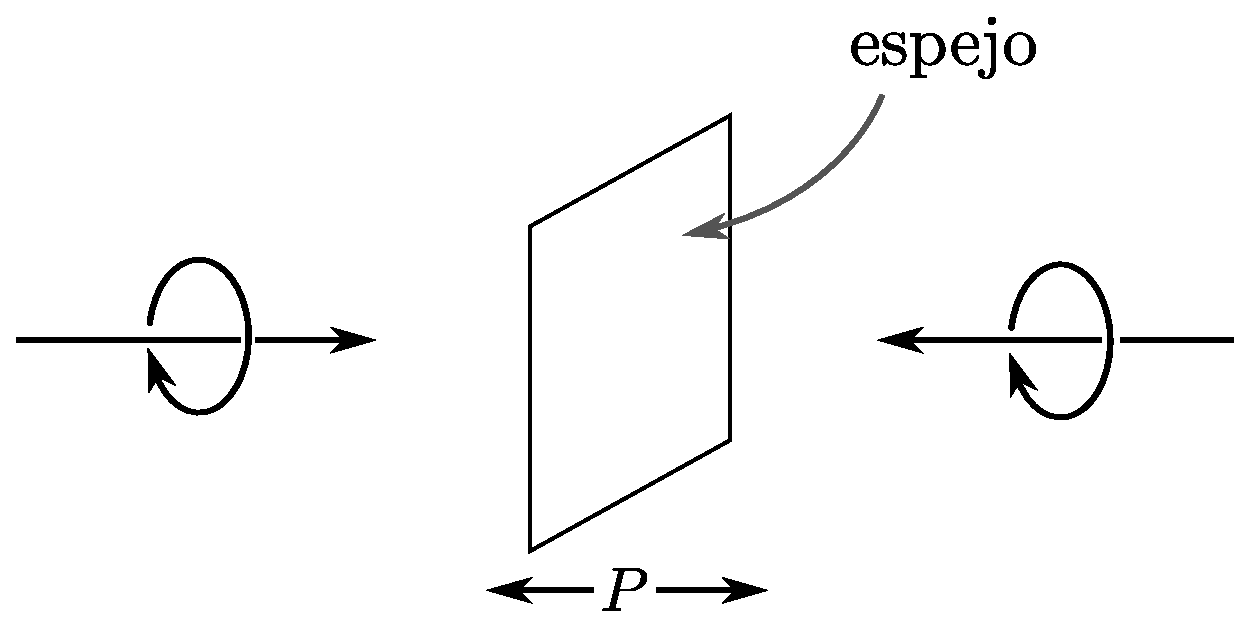
\includegraphics[scale=0.3]{Capitulos/Apendices/paridad.eps}
    \caption{La reflexión de un vector y un pseudovector apuntando perpendicularmente a un espejo ilustran una transformación de paridad en esa dirección.}
    \label{paridad}
\end{figure}

Sin embargo, podemos definir el campo de Dirac, de cuatro componentes complejas:
\begin{equation}
    \psi(x) = \mqty( \psi_{L}(x) \\ \psi_{R}(x) ),
\end{equation}
que bajo transformaciones de Lorentz (ortocronas propias) $x^{\mu} \mapsto x^{\prime \mu}=\Lambda^{\mu}_{~\nu}x^{\nu}$,
\begin{equation}
    \psi(x) \mapsto \psi^{\prime}(x^{\prime})=\Lambda_{D}\psi(x), \quad \Lambda_{D}= \smqty(\Lambda_{L} & 0 \\ 0 & \Lambda_{R}),
\end{equation}
y bajo paridad, $x^{\mu}=(t,\vb*{x}) \mapsto \tilde{x}^{\mu}=(t,-\vb*{x})$,
\begin{equation}
    \psi(x) \mapsto \psi^{\prime}(\tilde{x})=\mqty( \psi_{R}(\tilde{x}) \\ \psi_{L}(\tilde{x}) )=\mqty(0 & \vb*{1} \\ \vb*{1} & 0)\psi(\tilde{x}). 
\end{equation}

El conjugado de carga de un espinor de Dirac es otro espinor de Dirac,
\begin{equation}
    \psi^{c}=\mqty( \psi^{c}_{R}(x) \\ \psi^{c}_{L}(x) ) = \mqty( -\ii \sigma^{2}\psi_{R}^{*} \\ \ii \sigma^{2}\psi_{L}^{*})=-\ii \mqty( 0 & \sigma^2 \\ -\sigma^2 & 0 )\psi^{*}
\end{equation}

y, por supuesto , $\qty\big(\psi^{c})^{c} = \psi$. Además note que las coordenadas $x^{\mu}$ no cambian bajo conjugación de carga.\\

Los campos de Dirac y no los de Weyl son los objetos básicos en las teorías de campos invariantes bajo paridad, como la QED y la QCD.\\

Finalmente, un \emph{espinor de Majorana} es un espinor de Dirac en el que $\psi_L$ y $\psi_R$ no son independientes sino que

\begin{equation}
    \psi_R=\zeta \ii \sigma^2 \psi_L^* \quad \Rightarrow \quad \psi_M=\mqty(\psi_L \\ \zeta \ii \sigma^2 \psi_L^*), \quad  \abs{\zeta}^2=1.
\end{equation}

Tiene dos grados de libertad, como un espinor de Weyl, pero es autoconjugado de carga,

\begin{equation}
    \psi_M^c=\mqty(\zeta^* \psi_L \\ \ii \sigma^2 \psi_L^*) = \zeta^* \psi_M.
\end{equation}

\subsection{Campos vectoriales}

Bajo transformaciones de Lorentz, los campos vectoriales cumplen

\begin{equation}
    V^\mu(x) \mapsto V^{\prime \mu}\left(x^{\prime}\right)=\Lambda_\nu^\mu V^v(x) .
\end{equation}

Entonces, a partir de (\ref{eq_A103}) y (\ref{eq_A106}),

\begin{equation}
    \delta V^\mu(x)=\qty(\Lambda_{~\nu}^\mu-\delta_\nu^\mu) V^\nu(x)-\frac{\ii}{2} \omega_{\rho \sigma} L^{\rho \sigma} V^\mu(x) \equiv-\frac{\ii}{2} \omega_{\rho \sigma} J_V^{\rho \sigma} V^\mu(x) .
\end{equation}


Si escribimos, como antes, $J_V^{\rho \sigma}=L^{\rho \sigma}+S_V^{\rho \sigma}$, vemos que

\begin{equation}
    \Lambda_{~\nu}^\mu-\delta_{\nu}^\mu \equiv-\frac{\ii}{2} \omega_{\rho \sigma}\qty(S_V^{\rho \sigma})^{\mu}_{~\nu}=-\frac{\ii}{2} \omega_{\rho \sigma}\qty(J^{\rho \sigma})_{~\nu}^{\mu} \quad \Rightarrow \quad S_V^{\rho \sigma}=J^{\rho \sigma}.
\end{equation}

\section{Grupo de Poincare}

El grupo de Poincaré incluye las transformaciones de Lorentz y las traslaciones espacio-temporales,

\begin{equation}
    x^\mu \mapsto x^{\prime \mu}=x^\mu+a^\mu.
    \label{eq_A124}
\end{equation}

Si tomamos una traslación infinitesimal $a^\mu=\epsilon^\mu$,

\begin{IEEEeqnarray}{rCl}
    x^{\prime \mu} \equiv\qty(\vb*{1}-\mathrm{i} \epsilon_\rho P^\rho ) x^\mu & ~~\Rightarrow~~ & \delta x^\mu=\epsilon^\mu=-\mathrm{i} \epsilon_\rho P^\rho x^\mu \\
    & ~~\Rightarrow~~  & \quad P^\rho=\ii \partial^\rho .
\end{IEEEeqnarray}


Así que los generadores de las traslaciones son las 4 componentes del operador cuadrimomento $P^\mu$. La traslación (\ref{eq_A124}) se escribe, por tanto, $\exp (-\ii a_\mu P^\mu)$.\\

El álgebra de Poincaré, escrita en forma covariante, es

\begin{IEEEeqnarray}{rCl}
    \comm{P^\mu}{p^\nu} & = & 0, \\
    \comm{P^\mu}{J^{\rho \sigma}} & = & \ii \qty( g^{\mu \rho} P^\sigma-g^{\mu \sigma} P^\rho ),\\ \label{eq_A1.100}
    \comm{J^{\mu \nu}}{J^{\rho \sigma}} & = & \ii \qty(g^{\nu \rho}J^{\mu \sigma}  - g^{\mu \rho}J^{\nu \sigma}  - g^{\nu \sigma}J^{\mu \rho}  +g^{\mu \sigma}J^{\nu \rho} ).
\end{IEEEeqnarray}

La última línea corresponde al álgebra del subgrupo de Lorentz (\ref{eq_A106}). Las traslaciones son también un subgrupo. Conviene explicitar las relaciones de conmutación entre los generadores de las traslaciones y los de rotaciones y boosts:

\begin{IEEEeqnarray}{rCl}
    \comm{P^0}{J^k} & = & 0, \\
    \comm{P^k}{J^l} & = & \ii \epsilon^{klm} P^{m}, \\ 
    \comm{P^0}{K^k} & = & \ii P^k, \\
    \comm{P^k}{K^l} & = & \ii P^0 \delta^{kl}. 
\end{IEEEeqnarray}

Así que, como el hamiltoniano es $H = P^0$ (generador de las traslaciones temporales), tenemos que $\comm{H}{P^k}=\comm{H}{J^k}=0$ pero $\comm{H}{K^k} \neq 0$. Esto no significa que solo momento lineal y momento angular total son cantidades conservadas, porque $K^i$ depende explícitamente del tiempo de tal forma que

\begin{equation}
    \dv{x} K^k = \ii \comm{H}{K^k}+\pdv{t}K^k=0.
\end{equation}
Así que también hay cantidades conservadas asociadas a los boots, como se vió al estudiar el teorema de Noether en el siguiente tema.

\subsection{Representaciones sobre los campos}

Ya hemos visto que los campos forman representaciones de dimensión infinita del grupo de Lorentz, con generadores

\begin{equation}
    J^{\mu \nu}=L^{\mu \nu}+S^{\mu \nu},
    \label{eq_A1.107}
\end{equation}

donde $L^{\mu \nu}=\ii \qty(x^\mu \partial^\nu-x^\nu \partial^\mu )$ y $S^{\mu \nu}$ depende de si el campo es escalar, espinorial, etc. Hallemos ahora la representación de las traslaciones. Para ello, imponemos que para cualquier componente, ya sea tensorial o espinorial del campo, se cumple

\begin{equation}
    \phi^{\prime}\left(x^{\prime}\right)=\phi(x), \quad x^{\prime \mu}=x^\mu+a^\mu.
\end{equation}

Entonces, haciendo una translación infinitesimal $a^\mu=\epsilon^\mu$,

\begin{equation}
    \delta \phi(x) \equiv \phi^{\prime}(x) -  \phi (x) = \phi^{\prime}\left(x^{\prime}-\epsilon\right)-\phi(x)=\phi^{\prime}\left(x^{\prime}\right)-\epsilon^\mu \partial_\mu \phi(x)-\phi(x)=-\epsilon^\mu \partial_\mu \phi(x).
\end{equation}

Por tanto, comparando esta expresión con

\begin{equation}
    \phi^{\prime}\left(x^{\prime}-\epsilon\right)=\exp \left\{-\mathrm{i}\left(-\epsilon_\mu\right) P^\mu\right\} \phi^{\prime}\left(x^{\prime}\right) \Rightarrow \delta \phi(x)=\mathrm{i} \epsilon_\mu P^\mu \phi(x)
\end{equation}

tenemos que

\begin{equation}
    P^\mu=\ii \partial^\mu .
    \label{eq_A1.111}
\end{equation}

Para ver que lo que hemos obtenido es consistente, podemos comprobar la regla de conmutación (\ref{eq_A1.100}) usando la representación sobre campos de los generadores del grupo de Lorentz (\ref{eq_A1.107}) y de las traslaciones (\ref{eq_A1.111}) y teniendo en cuenta que $S^{\mu \nu}$ es independiente de las coordenadas espacio-temporales y por tanto conmuta con $\partial^\mu$,

\begin{IEEEeqnarray}{rCl}
    \comm{P^\mu}{J^{\rho \sigma}} = \comm{P^\mu}{L^{\rho \sigma}} &=& \left[\ii \partial^\mu, \ii \left(x^\rho \partial^\sigma-x^\sigma \partial^\rho\right)\right] \\
    &=&-\left(g^{\mu \rho} \partial^\sigma-g^{\mu \sigma} \partial^\rho \right)=\ii \left(g^{\mu \rho} P^\sigma-g^{\mu \sigma} P^\rho \right),
\end{IEEEeqnarray}

donde hemos aplicado la regla $\comm{A}{BC}=\comm{A}{B}C+A\comm{B}{C}$ y sustituido $\left[\partial^\mu, x^\nu\right]=g^{\mu \nu}$.

%-----------------
\subsection{Representaciones sobre estados de una partícula}

Ya hemos visto todo lo que necesitamos para construir lagrangianos de campos invariantes bajo Poincaré. Cuando se cuantizan los campos veremos que éstos crean y destruyen partículas (y antipartículas). Es conveniente entonces identificar el espacio de Hilbert de estados de una partícula, invariante bajo Poincaré, es decir, irreps del grupo de Poincaré etiquetadas por sus operadores de Casimir y cuyos vectores vienen especificados por números cuánticos que son autovalores de un conjunto de generadores que conmuten entre sí (y de otros operadores que conmuten con ellos), $\ket{\vb*{p},j_{3},\ldots}$.\\

El grupo de Poincaré tiene dos operadores de Casimir:

\begin{equation}
    m^2=P_\mu P^\mu \quad \mathrm{y} \quad W_\mu W^\mu,
\end{equation}

donde $W^\mu$ es el cuadrivector de \emph{Pauli-Lubanski} definido por
\begin{equation}
   W^\mu=-\frac{1}{2} \epsilon^{\mu \nu \rho \sigma} J_{\nu \rho} P_\sigma . 
\end{equation}

Ambos operadores conmutan, pues

\begin{IEEEeqnarray}{rCl}
    \comm{W^\mu}{P^\alpha} & = & -\frac{1}{2} \epsilon^{\mu \nu \rho \sigma}\comm{J_{\nu \rho} P_\sigma}{P^\alpha}\\
    &=&-\frac{1}{2} \epsilon^{\mu \nu \rho \sigma}\left(J_{v \rho}\comm{P_\sigma}{P^\alpha} +\comm{J_{v \rho}}{ P^\alpha}P_\sigma\right) \\
    &=&-\frac{\ii}{2} \epsilon^{\mu \nu \rho \sigma}\left(g_\rho^\alpha P_\nu-g_\nu^\alpha P_\rho\right) \\
    &=&-\frac{\ii}{2} \epsilon^{\mu v \alpha \sigma} P_v+\frac{\ii}{2} \epsilon^{\mu \alpha \rho \sigma} P_\rho=0 .
\end{IEEEeqnarray}

Además $m^2=P_\mu P^\mu$ y $W_\mu W^\mu$ son invariantes Lorentz. Por tanto, son operadores de Casimir (conmutan con $P^\rho$ y $J^{\rho \sigma}$ ) y podemos usar sus autovalores para etiquetar las irreps y calcularlos en el sistema de referencia que queramos. Tenemos que distinguir dos casos:

\begin{itemize}
    \item Caso $m \neq 0$ \\
    
    Usemos el sistema de referencia en reposo, $p^\mu=(m, 0,0,0)$. Entonces,

    \begin{equation}
        \left.\begin{array}{l}
        W^0=0 \\
        W^i=-\frac{m}{2} \epsilon^{i j k 0} J^{j k}=\frac{m}{2} \epsilon^{i j k} J^{j k}=m J^i
        \end{array}\right\} \quad \Rightarrow \quad W_\mu W^\mu=-m^2 j(j+1) .
    \end{equation}
    Es decir, las irreps están etiquetadas por $m, j$ y los vectores por $\ket{j_3=-j \ldots j}$, donde $j$ es el espín. Vemos que las partículas masivas de espín $j$ tienen $2 j+1$ grados de libertad. Esto es así porque, una vez que se ha hecho un boost para llevar la partícula masiva al sistema de referencia en el que su cuadrimomento es $p^\mu=(m, 0,0,0)$, tenemos total libertad para rotar en tres dimensiones el sistema. Decimos que el grupo $\SU2$ es su grupo de Lorentz pequeño (conjunto de transformaciones de Lorentz que dejan invariante una elección dada de $p^\mu$).
    \vspace{0.5cm}

    \item Caso $m=0$\\
    
    No existe el sistema de referencia en reposo. Podemos elegir uno en el que $p^\mu=(\omega, 0,0, \omega)$, que describe una partícula sin masa que se mueve en la dirección del eje $z$. Entonces,

    \begin{equation}
        \left.\begin{array}{rl}
        -W^0 & =W^3=\omega J^3 \\
        W^1 & =\omega\left(J^1+K^2\right) \\
        W^2 & =\omega\left(J^2-K^1\right)
        \end{array}\right\} 
        \quad \Rightarrow \quad W_\mu W^\mu=-\omega^2\left[\left(J^1+K^2\right)^2+\left(J^2-K^1\right)^2\right].
    \end{equation}
    En este caso el grupo pequeño son las rotaciones en el plano perpendicular a la dirección del movimiento (el plano $(x, y)$ en nuestra elección), que es $\SO2$, cuyas irreps son unidimensionales (grupo abeliano) y se etiquetan por un número $h \in\left\{0, \pm \frac{1}{2}, \pm 1, \ldots\right\}$ llamado helicidad (proyección del momento angular en la dirección del movimiento):\footnote{Los elementos de $\SO2$ en la irrep $h$ vienen dados por $R(\theta) = \exp \qty( - \ii h\theta)$.}

    \begin{equation}
        h=\hat{\vb*{p}} \cdot \vb*{J}.
    \end{equation}
    
    Nótese que $h=j_3$ en nuestra elección de dirección del movimiento, con $j_3=\pm j$. Las irreps $h$ y $-h$ son distintas (no se mezclan bajo transformaciones de Poincaré), aunque en las teorías simétricas bajo paridad las partículas sin masa correspondientes reciben el mismo nombre y se dice que están en dos estados distintos de helicidad. Así se habla de fotón ( $m=0, j=1$ ) dextrógiro/levógiro si $h=\pm 1$. También decimos que el fotón es una partícula sin masa de espín $1$, aunque en realidad no existe el estado con $j_3=0$. Del mismo modo, veremos que los campos de Weyl sin masa $\psi_L$ y $\psi_R$ $\left(m=0, j=\frac{1}{2}\right)$ tienen helicidad $h=-\frac{1}{2}$, $h=+\frac{1}{2}$, respectivamente y representan a partículas distintas si la teoría no es simétrica bajo paridad (e.g. en el modelo estándar si los neutrinos no tienen masa el neutrino es $\nu_L$ y el $\nu_R$ podría no existir).
    
    Un último comentario: siempre podemos hablar de helicidad como la proyección del momento angular en la dirección del movimiento, pero solamente es una cantidad invariante bajo transformaciones de Poincaré para partículas sin masa. A veces se usa el término quiralidad, que tiene que ver con si la partícula se transforma bajo la representación del espinor izquierdo o del espinor derecho del grupo de Lorentz. La quiralidad coincide con la helicidad para partículas sin masa.
\end{itemize}

\begin{cabox}
    \textbf{Aspectos para llevarse de esta sección}
    \renewcommand{\labelitemi}{\ding{42}}
    \begin{itemize}
        \item Grupos para recordar: grupo de Lorentz y subgrupos, grupo de Poincaré.
        \item $so(3,1)=su(2)+su(2) \Longrightarrow$ Irreps de $\mathrm{SO}(3,1)$ se etiquetan por $\left(j_1, j_2\right)$ (espín de cada $su(2)$).
        \item Un espinor es un elemento sobre el cual actúa la irrep de $s u(2)$ de $j=1/2$.
        \item Espinor de Weyl 
              $\begin{cases}
              \text{izquierdo} \rightarrow\left(\frac{1}{2}, 0\right)\\ 
              \text{derecho} \rightarrow \left(0, \frac{1}{2}\right) 
              \end{cases}$
        \item Las irreps del grupo de Poincaré van a estar asociadas al concepto de partícula elemental en nuestra teoría.
    \end{itemize}
\end{cabox}



%-----------------------------------------------      Fin Capítulo 1 -------------------------------------------------------------------------------------------
%\chapterimage{chapter_head_2.pdf} % Chapter heading image
\label{Apendice B}

\chapter{Ecuaciones de Campo E-L}

En este apéndice se da a conocer una manera alternativa de derivar las ecuaciones de Euler-Lagrange.
Se considera un conjunto uniparam\'{e}trico de funciones variadas que se reducen al valor correcto de $\phi
_{r}\left( x \right) $ cuando $\alpha $ va a cero. Una familia de estas funciones se puede constru\'{\i}r como:

\begin{equation*}
\phi_{r}\left( x,\alpha \right) =\phi_{r}\left( x,0\right) +\alpha \zeta _{r}\left( x\right) ~,
\end{equation*}

las funciones $\zeta_{r}\left(x\right)$ son funciones de clase $C^{2}$ en todos los par\'{a}metros. Dichas funciones se deben anular sobre la hipersuperficie $\Sigma$ que delimita a la regi\'{o}n de integraci\'{o}n. La anulaci\'{o}n del variacional de $S$, es equivalente a establecer
que la derivada de $S$ con respecto a $\alpha $ sea cero.

\begin{equation}
\frac{dS}{d\alpha }=\frac{d}{d\alpha }\int d^{4}x\ \mathcal{L}\left(\phi_{r},\partial_{\mu }\phi_{r},x\right) =\int d^{4}x\
\left\{ \frac{\partial \mathcal{L}}{\partial \phi_{r}}\frac{\partial \phi _{r}}{\partial \alpha }\mathcal{+}\frac{\partial \mathcal{L}}{\partial \left( \partial _{\mu }\phi_{r}\right) }\frac{\partial \left(\partial _{\mu }\phi _{r}\right) }{\partial \alpha }\right\} ~.
\label{2.19}
\end{equation}
integrando por partes se obtiene,
\begin{equation}
\frac{dS}{d\alpha }=\int d^{4}x\ \frac{\partial \phi_{r}}{\partial \alpha }\left\{ \frac{\partial \mathcal{L}}{\partial \phi_{r}}-\partial
_{\mu}\left( \frac{\partial \mathcal{L}}{\partial \left( \partial _{\mu }\phi_{r}\right) }\right) \right\} +\int d^{4}x\partial_{\mu}\left(\frac{\partial \mathcal{L}}{\partial \left( \partial _{\mu }\phi_{r}\right) }\frac{\partial \phi_{r}}{\partial \alpha }\right)
~.  \label{2.19a}
\end{equation}

La segunda integral se elimina cuando $\alpha $ tiende a cero, lo cual se
puede ver de varias formas:
\vspace{0.5cm}

\begin{itemize}
\item Si se observa t\'{e}rmino a t\'{e}rmino, al realizar la integraci\'{o}n sobre un parámetro $x$ en particular para cada t\'{e}rmino de la derivada, se v\'{e} que estos t\'{e}rminos se tienen que desaparecer porque la derivada con respecto a $\alpha $ de los campos es cero en los extremos.\\


\item La integral se puede transformar por medio de un teorema de la
divergencia en 4 dimensiones en una integral sobre la hipersuperficie que
delimita la regi\'{o}n de integraci\'{o}n en el cuadriespacio (\textbf{euclidiano})\footnote{Procedimiento realizado en el desarrollo teórico en la variación de la acción}. La integral de superficie tambi\'{e}n se anula porque la variaci\'{o}n de $\phi_{r}$ en la vecindad de la funci\'{o}n de campo correcta es cero sobre la superficie. Para ver esto se calcula la segunda integral a la derecha en (\ref{2.19a}), as\'{\i}
\end{itemize}

\begin{eqnarray}
\int d^{4}x~\partial _{\mu }\left( \frac{\partial \mathcal{L}}{\partial
\left( \partial _{\mu }\phi _{r}\right) }\frac{\partial \phi _{r}}{\partial
\alpha }\right)  &=&\int d^{4}x~\left[ \partial _{0}\left( \frac{\partial 
\mathcal{L}}{\partial \left( \partial _{0}\phi _{r}\right) }\frac{\partial
\phi _{r}}{\partial \alpha }\right) +\partial _{i}\left( \frac{\partial 
\mathcal{L}}{\partial \left( \partial _{i}\phi _{r}\right) }\frac{\partial
\phi _{r}}{\partial \alpha }\right) \right]   \notag \\
&=&\int d^{4}x\partial _{0}\left( \frac{\partial \mathcal{L}}{\partial
\left( \partial _{0}\phi _{r}\right) }\frac{\partial \phi _{r}}{\partial
\alpha }\right) +\int d^{4}x\partial _{i}\left( \frac{\partial \mathcal{L}}{%
\partial \left( \partial _{i}\phi _{r}\right) }\frac{\partial \phi _{r}}{%
\partial \alpha }\right)   \notag \\
&=&\int d^{3}x\int_{t_{1}}^{t_{2}}dt~\partial _{0}\left( \frac{\partial 
\mathcal{L}}{\partial \left( \partial _{\mu }\phi _{r}\right) }\frac{%
\partial \phi _{r}}{\partial \alpha }\right)   \notag \\
&&+\int_{t_{1}}^{t_{2}}dt~\int d^{3}x~\partial _{i}\left( \frac{\partial 
\mathcal{L}}{\partial \left( \partial _{i}\phi _{r}\right) }\frac{\partial
\phi _{r}}{\partial \alpha }\right)   \notag \\
&=&\int d^{3}x~\left. \left( \frac{\partial \mathcal{L}}{\partial \left(
\partial _{\mu }\phi _{r}\right) }\frac{\partial \phi _{r}}{\partial \alpha }%
\right) \right\vert _{t_{1}}^{t_{2}}  \notag \\
&&+\int_{t_{1}}^{t_{2}}dt~\int d^{3}x~\partial _{i}\left( \frac{\partial 
\mathcal{L}}{\partial \left( \partial _{i}\phi _{r}\right) }\frac{\partial
\phi _{r}}{\partial \alpha }\right) ~.
\end{eqnarray}

De este resultado se establece que la primera integral se anula por la
condici\'{o}n de frontera $\left. \frac{\partial \phi_{r}}{\partial
\alpha }\right\vert _{t=t_{1}}=\left. \frac{\partial \phi_{r}}{\partial
\alpha }\right\vert _{t=t_{2}}=0$. De igual manera, en la segunda integral
el integrando esta siendo evaluado en la superficie que encierra el volumen en el cual est\'{a} siendo considerados los campos. Si este volumen se extiende en todo el espacio, la superficie que lo limita tiende a infinito y del comportamiento asint\'{o}tico de los campos hace que esta integral de superficie tienda a cero, es decir

\begin{equation*}
\int_{t_{1}}^{t_{2}}dt\int d^{3}x~\partial _{i}\left( \frac{\partial \mathcal{L}}{\partial \left( \partial _{i}\phi_{r}\right) }\frac{\partial\phi_{r}}{\partial \alpha }\right)=\int_{t_{1}}^{t_{2}}dt\oint_{S}ds_{i}\left(\frac{\partial \mathcal{L}}{\partial \left( \partial _{i}\phi_{r}\right) }\zeta_{r}\right) =0~\  .
\end{equation*}

\noindent
De esta manera, se deduce que la variaci\'{o}n 

\begin{equation}
\delta \int d^{4}x\ \partial _{\mu }\left( \frac{\partial \mathcal{L}}{%
\partial \left( \partial _{\mu }\phi_{r}\right) }\frac{\partial \phi
_{r}}{\partial \alpha }\right) =\delta \int d^{4}x\ \partial _{\mu
}\left( \frac{\partial \mathcal{L}}{\partial \left( \partial _{\mu }\phi
_{r}\right) }\zeta _{r}\right) =0 ~.  \label{2.21}
\end{equation}

\noindent
Por lo anterior, en el l\'{\i}mite cuando $\alpha \rightarrow 0$, la ecuaci\'{o}n (\ref{2.19a}) se reduce a,

\begin{equation}
\left( \frac{dS}{d\alpha }\right) _{\alpha =0}=\int d^{4}x\ \left( \frac{\partial \phi_{r}}{\partial \alpha }\right) _{\alpha =0}\left\{ \frac{\partial \mathcal{L}}{\partial \phi _{r}}-\partial _{\mu }\left( \frac{\partial \mathcal{L}}{\partial \left( \partial _{\mu }\phi_{r}\right) }\right) \right\} =0~,  \label{2.21a}
\end{equation}
y de la naturaleza arbitraria de la variaci\'{o}n de cada campo $\phi_{r}$, la ecuaci\'{o}n (\ref{2.21a}) se satisface s\'{o}lo si se anula el t\'{e}rmino entre llaves, entonces del lema fundamental del c\'{a}lculo de variaciones se determina,

\begin{equation}
\frac{\partial \mathcal{L}}{\partial \phi_{r}}-\partial _{\mu }\left(\frac{\partial \mathcal{L}}{\partial \left( \partial _{\mu }\phi _{r}\right) }\right) =0~.  \label{2.22}
\end{equation}

La relaci\'{o}n (\ref{2.22}) es conocida como ecuaci\'{o} de
Euler-Lagrange, y representa un conjunto de ecuaciones diferenciales
parciales para las variables de campo, el n\'{u}mero de ecuaciones est\'{a} determinado por los valores posibles de $r$. Vale la pena enfatizar de nuevo que dado que cada $x$ corresponde a un \'{\i}ndice continuo para las variables de campo. Cada una de las ecuaciones (\ref{2.22}) para $r$ fijo, corresponde a un conjunto completo de ecuaciones diferenciales de movimiento de Lagrange en el caso discreto.

\begin{exercise}
Utilizar integraci\'{o}n por partes para demostrar la ecuaci\'{o}n (\ref%
{2.19a}).
\end{exercise}

\begin{solution}
Al utilizar la integraci\'{o}n por partes%
\begin{eqnarray*}
\int dx^{\mu }\partial _{\nu }\left( \frac{\partial \mathcal{L}}{\partial
\eta _{\rho ,\nu }}\frac{\partial \eta _{\rho }}{\partial \alpha }\right)
&=&\int dx^{\mu }\partial _{\nu }\left( \frac{\partial \mathcal{L}}{\partial
\left( \partial _{\nu }\eta _{\rho }\right) }\right) \frac{\partial \eta
_{\rho }}{\partial \alpha }+\int dx^{\mu }\frac{\partial \mathcal{L}}{%
\partial \left( \partial _{\nu }\eta _{\rho }\right) }\partial _{\nu }\left( 
\frac{\partial \eta _{\rho }}{\partial \alpha }\right) \\
&=&\int dx^{\mu }\partial _{\nu }\left( \frac{\partial \mathcal{L}}{\partial
\left( \partial _{\nu }\eta _{\rho }\right) }\right) \frac{\partial \eta
_{\rho }}{\partial \alpha }+\int dx^{\mu }\frac{\partial \mathcal{L}}{%
\partial \eta \left( \partial _{\nu }\eta _{\rho }\right) }\frac{\partial
\left( \partial _{\nu }\eta _{\rho }\right) }{\partial \alpha }~~~~~,
\end{eqnarray*}%
de manera que:%
\begin{equation*}
\int dx^{\mu }\frac{\partial \mathcal{L}}{\partial \left( \partial _{\nu
}\eta _{\rho }\right) }\frac{\partial \left( \partial _{\nu }\eta _{\rho
}\right) }{\partial \alpha }=\int dx^{\mu }\left[ \partial _{\nu }\left( 
\frac{\partial \mathcal{L}}{\partial \left( \partial _{\nu }\eta _{\rho
}\right) }\frac{\partial \eta _{\rho }}{\partial \alpha }\right) -\partial
_{\nu }\left( \frac{\partial \mathcal{L}}{\partial \left( \partial _{\nu
}\eta _{\rho }\right) }\right) \frac{\partial \eta _{\rho }}{\partial \alpha 
}\right] ~~~~~,
\end{equation*}%
lo que implica en (\ref{2.19})%
\begin{eqnarray}
\frac{dS}{d\alpha } &=&\int dx^{\mu }\ \left\{ \frac{\partial \mathcal{L}}{%
\partial \eta _{\rho }}\frac{\partial \eta _{\rho }}{\partial \alpha }%
\mathcal{+}\partial _{\nu }\left( \frac{\partial \mathcal{L}}{\partial
\left( \partial _{\nu }\eta _{\rho }\right) }\frac{\partial \eta _{\rho }}{%
\partial \alpha }\right) -\partial _{\nu }\left( \frac{\partial \mathcal{L}}{%
\partial \left( \partial _{\nu }\eta _{\rho }\right) }\right) \frac{\partial
\eta _{\rho }}{\partial \alpha }\right\}  \notag \\
&=&\int dx^{\mu }\ \frac{\partial \eta _{\rho }}{\partial \alpha }\left\{ 
\frac{\partial \mathcal{L}}{\partial \eta _{\rho }}-\partial _{\nu }\left( 
\frac{\partial \mathcal{L}}{\partial \left( \partial _{\nu }\eta _{\rho
}\right) }\right) \right\} +\int dx^{\mu }\partial _{\nu }\left( \frac{%
\partial \mathcal{L}}{\partial \left( \partial _{\nu }\eta _{\rho }\right) }%
\frac{\partial \eta _{\rho }}{\partial \alpha }\right) ~~~~~.  \label{2.20}
\end{eqnarray}
\end{solution}


\end{document}
